\documentclass{book}
\usepackage[a4paper,top=2.5cm,bottom=2.5cm,left=2.5cm,right=2.5cm]{geometry}
\usepackage{makeidx}
\usepackage{natbib}
\usepackage{graphicx}
\usepackage{multicol}
\usepackage{float}
\usepackage{listings}
\usepackage{color}
\usepackage{ifthen}
\usepackage[table]{xcolor}
\usepackage{textcomp}
\usepackage{alltt}
\usepackage{ifpdf}
\ifpdf
\usepackage[pdftex,
            pagebackref=true,
            colorlinks=true,
            linkcolor=blue,
            unicode
           ]{hyperref}
\else
\usepackage[ps2pdf,
            pagebackref=true,
            colorlinks=true,
            linkcolor=blue,
            unicode
           ]{hyperref}
\usepackage{pspicture}
\fi
\usepackage[utf8]{inputenc}
\usepackage{mathptmx}
\usepackage[scaled=.90]{helvet}
\usepackage{courier}
\usepackage{sectsty}
\usepackage{amssymb}
\usepackage[titles]{tocloft}
\usepackage{doxygen}
\lstset{language=C++,inputencoding=utf8,basicstyle=\footnotesize,breaklines=true,breakatwhitespace=true,tabsize=4,numbers=left }
\makeindex
\setcounter{tocdepth}{3}
\renewcommand{\footrulewidth}{0.4pt}
\renewcommand{\familydefault}{\sfdefault}
\hfuzz=15pt
\setlength{\emergencystretch}{15pt}
\hbadness=750
\tolerance=750
\begin{document}
\hypersetup{pageanchor=false,citecolor=blue}
\begin{titlepage}
\vspace*{7cm}
\begin{center}
{\Large Net\-Game \\[1ex]\large \hyperlink{class_game}{Game} Servers }\\
\vspace*{1cm}
{\large Generated by Doxygen 1.8.3.1}\\
\vspace*{0.5cm}
{\small Mon Apr 15 2013 04:06:03}\\
\end{center}
\end{titlepage}
\clearemptydoublepage
\pagenumbering{roman}
\tableofcontents
\clearemptydoublepage
\pagenumbering{arabic}
\hypersetup{pageanchor=true,citecolor=blue}
\chapter{Deprecated List}
\label{deprecated}
\hypertarget{deprecated}{}

\begin{DoxyRefList}
\item[\label{deprecated__deprecated000001}%
\hypertarget{deprecated__deprecated000001}{}%
Member \hyperlink{class_json_1_1_reader_afa4a59e962d23c4d1c38b433fc95eefa}{Json\-:\-:Reader\-:\-:get\-Formated\-Error\-Messages} () const ]Use get\-Formatted\-Error\-Messages() instead (typo fix). 
\end{DoxyRefList}
\chapter{Namespace Index}
\section{Namespace List}
Here is a list of all documented namespaces with brief descriptions\-:\begin{DoxyCompactList}
\item\contentsline{section}{\hyperlink{namespace_json}{Json} \\*J\-S\-O\-N (Java\-Script Object Notation) }{\pageref{namespace_json}}{}
\item\contentsline{section}{\hyperlink{namespace_network}{Network} \\*Some convenience functions }{\pageref{namespace_network}}{}
\end{DoxyCompactList}

\chapter{Hierarchical Index}
\section{Class Hierarchy}
This inheritance list is sorted roughly, but not completely, alphabetically\-:\begin{DoxyCompactList}
\item \contentsline{section}{Hash\-:\-:\-\_\-ht}{\pageref{struct_hash_1_1__ht}}{}
\item \contentsline{section}{Agg\-Info}{\pageref{struct_agg_info}}{}
\item \contentsline{section}{Agg\-Info\-:\-:Agg\-Info\-\_\-col}{\pageref{struct_agg_info_1_1_agg_info__col}}{}
\item \contentsline{section}{Agg\-Info\-:\-:Agg\-Info\-\_\-func}{\pageref{struct_agg_info_1_1_agg_info__func}}{}
\item \contentsline{section}{analysis\-Info}{\pageref{structanalysis_info}}{}
\item \contentsline{section}{Attach\-Key}{\pageref{struct_attach_key}}{}
\item \contentsline{section}{Auth\-Context}{\pageref{struct_auth_context}}{}
\item \contentsline{section}{Autoinc\-Info}{\pageref{struct_autoinc_info}}{}
\item \contentsline{section}{Vdbe\-Func\-:\-:Aux\-Data}{\pageref{struct_vdbe_func_1_1_aux_data}}{}
\item \contentsline{section}{Json\-:\-:Batch\-Allocator$<$ Allocated\-Type, object\-Per\-Allocation $>$}{\pageref{class_json_1_1_batch_allocator}}{}
\item \contentsline{section}{Bitvec}{\pageref{struct_bitvec}}{}
\item \contentsline{section}{Bt\-Cursor}{\pageref{struct_bt_cursor}}{}
\item \contentsline{section}{Bt\-Lock}{\pageref{struct_bt_lock}}{}
\item \contentsline{section}{Btree}{\pageref{struct_btree}}{}
\item \contentsline{section}{Bt\-Shared}{\pageref{struct_bt_shared}}{}
\item \contentsline{section}{Busy\-Handler}{\pageref{struct_busy_handler}}{}
\item \contentsline{section}{callback\-\_\-data}{\pageref{structcallback__data}}{}
\item \contentsline{section}{Cell\-Info}{\pageref{struct_cell_info}}{}
\item \contentsline{section}{Character}{\pageref{class_character}}{}
\begin{DoxyCompactList}
\item \contentsline{section}{Character\-Game\-Object}{\pageref{class_character_game_object}}{}
\begin{DoxyCompactList}
\item \contentsline{section}{Networked\-Character}{\pageref{class_networked_character}}{}
\begin{DoxyCompactList}
\item \contentsline{section}{Controlled\-Character}{\pageref{class_controlled_character}}{}
\end{DoxyCompactList}
\end{DoxyCompactList}
\end{DoxyCompactList}
\item \contentsline{section}{Client}{\pageref{class_client}}{}
\item \contentsline{section}{Clients\-Manager}{\pageref{class_clients_manager}}{}
\item \contentsline{section}{Coll\-Seq}{\pageref{struct_coll_seq}}{}
\item \contentsline{section}{Column}{\pageref{struct_column}}{}
\item \contentsline{section}{Command\-Handler}{\pageref{class_command_handler}}{}
\begin{DoxyCompactList}
\item \contentsline{section}{Game\-Command\-Handler}{\pageref{class_game_command_handler}}{}
\item \contentsline{section}{Server\-Command\-Handler}{\pageref{class_server_command_handler}}{}
\end{DoxyCompactList}
\item \contentsline{section}{compare\-Info}{\pageref{structcompare_info}}{}
\item \contentsline{section}{Controller}{\pageref{class_controller}}{}
\item \contentsline{section}{Count\-Ctx}{\pageref{struct_count_ctx}}{}
\item \contentsline{section}{Database\-Manager}{\pageref{class_database_manager}}{}
\item \contentsline{section}{Date\-Time}{\pageref{struct_date_time}}{}
\item \contentsline{section}{Db}{\pageref{struct_db}}{}
\item \contentsline{section}{Db\-Fixer}{\pageref{struct_db_fixer}}{}
\item \contentsline{section}{Debug}{\pageref{class_debug}}{}
\item \contentsline{section}{Distinct\-Ctx}{\pageref{struct_distinct_ctx}}{}
\item Drawable\begin{DoxyCompactList}
\item \contentsline{section}{Game\-Object}{\pageref{class_game_object}}{}
\begin{DoxyCompactList}
\item \contentsline{section}{Button}{\pageref{class_button}}{}
\item \contentsline{section}{Character\-Game\-Object}{\pageref{class_character_game_object}}{}
\item \contentsline{section}{G\-U\-I}{\pageref{class_g_u_i}}{}
\item \contentsline{section}{Target\-Block}{\pageref{class_target_block}}{}
\item \contentsline{section}{Text\-Input\-Field}{\pageref{class_text_input_field}}{}
\end{DoxyCompactList}
\end{DoxyCompactList}
\item \contentsline{section}{et\-\_\-info}{\pageref{structet__info}}{}
\item \contentsline{section}{Explain}{\pageref{struct_explain}}{}
\item \contentsline{section}{Expr}{\pageref{struct_expr}}{}
\item \contentsline{section}{Expr\-List}{\pageref{struct_expr_list}}{}
\item \contentsline{section}{Expr\-List\-:\-:Expr\-List\-\_\-item}{\pageref{struct_expr_list_1_1_expr_list__item}}{}
\item \contentsline{section}{Expr\-Span}{\pageref{struct_expr_span}}{}
\item \contentsline{section}{Json\-:\-:Features}{\pageref{class_json_1_1_features}}{}
\item \contentsline{section}{File\-Chunk}{\pageref{struct_file_chunk}}{}
\item \contentsline{section}{File\-Point}{\pageref{struct_file_point}}{}
\item \contentsline{section}{File\-Writer}{\pageref{struct_file_writer}}{}
\item \contentsline{section}{F\-Key}{\pageref{struct_f_key}}{}
\item \contentsline{section}{Full\-Expression\-Accumulator}{\pageref{class_full_expression_accumulator}}{}
\item \contentsline{section}{Func\-Def}{\pageref{struct_func_def}}{}
\item \contentsline{section}{Func\-Def\-Hash}{\pageref{struct_func_def_hash}}{}
\item \contentsline{section}{Func\-Destructor}{\pageref{struct_func_destructor}}{}
\item \contentsline{section}{Game}{\pageref{class_game}}{}
\item \contentsline{section}{Hash}{\pageref{struct_hash}}{}
\item \contentsline{section}{Hash\-Elem}{\pageref{struct_hash_elem}}{}
\item \contentsline{section}{Id\-List}{\pageref{struct_id_list}}{}
\item \contentsline{section}{Id\-List\-:\-:Id\-List\-\_\-item}{\pageref{struct_id_list_1_1_id_list__item}}{}
\item \contentsline{section}{Incrblob}{\pageref{struct_incrblob}}{}
\item \contentsline{section}{Index}{\pageref{struct_index}}{}
\item \contentsline{section}{Index\-Sample}{\pageref{struct_index_sample}}{}
\item \contentsline{section}{Init\-Data}{\pageref{struct_init_data}}{}
\item \contentsline{section}{Integrity\-Ck}{\pageref{struct_integrity_ck}}{}
\item \contentsline{section}{Key\-Info}{\pageref{struct_key_info}}{}
\item \contentsline{section}{Key\-State}{\pageref{class_key_state}}{}
\item \contentsline{section}{Level}{\pageref{class_level}}{}
\item \contentsline{section}{Like\-Op}{\pageref{struct_like_op}}{}
\item \contentsline{section}{Limit\-Val}{\pageref{struct_limit_val}}{}
\item \contentsline{section}{Local\-Player\-Info}{\pageref{class_local_player_info}}{}
\item \contentsline{section}{Login\-Data}{\pageref{struct_login_data}}{}
\item \contentsline{section}{Login\-Manager}{\pageref{class_login_manager}}{}
\item \contentsline{section}{Lookaside}{\pageref{struct_lookaside}}{}
\item \contentsline{section}{Lookaside\-Slot}{\pageref{struct_lookaside_slot}}{}
\item \contentsline{section}{Mem}{\pageref{struct_mem}}{}
\item \contentsline{section}{Mem\-Journal}{\pageref{struct_mem_journal}}{}
\item \contentsline{section}{Mem\-Page}{\pageref{struct_mem_page}}{}
\item \contentsline{section}{Module}{\pageref{struct_module}}{}
\item \contentsline{section}{Mutexes}{\pageref{class_mutexes}}{}
\item \contentsline{section}{Name\-Context}{\pageref{struct_name_context}}{}
\item \contentsline{section}{Network\-Event}{\pageref{class_network_event}}{}
\begin{DoxyCompactList}
\item \contentsline{section}{Create\-Target}{\pageref{class_create_target}}{}
\item \contentsline{section}{Destroy\-Target}{\pageref{class_destroy_target}}{}
\item \contentsline{section}{Load\-Level}{\pageref{class_load_level}}{}
\item \contentsline{section}{Player\-Accepted}{\pageref{class_player_accepted}}{}
\item \contentsline{section}{Player\-Event}{\pageref{class_player_event}}{}
\begin{DoxyCompactList}
\item \contentsline{section}{Player\-Authorize}{\pageref{class_player_authorize}}{}
\item \contentsline{section}{Player\-Connected}{\pageref{class_player_connected}}{}
\item \contentsline{section}{Player\-Disconnected}{\pageref{class_player_disconnected}}{}
\item \contentsline{section}{Player\-Send\-Message}{\pageref{class_player_send_message}}{}
\item \contentsline{section}{Player\-State\-Update}{\pageref{class_player_state_update}}{}
\end{DoxyCompactList}
\item \contentsline{section}{Player\-Rejected}{\pageref{class_player_rejected}}{}
\item \contentsline{section}{Player\-Update\-To\-Client}{\pageref{class_player_update_to_client}}{}
\item \contentsline{section}{Score\-Change}{\pageref{class_score_change}}{}
\item \contentsline{section}{Server\-Entry\-Accept}{\pageref{class_server_entry_accept}}{}
\item \contentsline{section}{Server\-Entry\-Add}{\pageref{class_server_entry_add}}{}
\item \contentsline{section}{Server\-Entry\-Get}{\pageref{class_server_entry_get}}{}
\item \contentsline{section}{Server\-Entry\-List}{\pageref{class_server_entry_list}}{}
\item \contentsline{section}{Server\-Entry\-Reject}{\pageref{class_server_entry_reject}}{}
\item \contentsline{section}{Target\-List}{\pageref{class_target_list}}{}
\end{DoxyCompactList}
\item Non\-Copyable\begin{DoxyCompactList}
\item \contentsline{section}{Config\-Loader}{\pageref{class_config_loader}}{}
\item \contentsline{section}{Game\-Object}{\pageref{class_game_object}}{}
\item \contentsline{section}{Master\-Server}{\pageref{class_master_server}}{}
\item \contentsline{section}{Network\-Interface}{\pageref{class_network_interface}}{}
\end{DoxyCompactList}
\item \contentsline{section}{Packet\-Wrap}{\pageref{struct_packet_wrap}}{}
\item \contentsline{section}{Pager}{\pageref{struct_pager}}{}
\item \contentsline{section}{Pager\-Savepoint}{\pageref{struct_pager_savepoint}}{}
\item \contentsline{section}{Parse}{\pageref{struct_parse}}{}
\item \contentsline{section}{Json\-:\-:Path}{\pageref{class_json_1_1_path}}{}
\item \contentsline{section}{Json\-:\-:Path\-Argument}{\pageref{class_json_1_1_path_argument}}{}
\item \contentsline{section}{P\-Cache}{\pageref{struct_p_cache}}{}
\item \contentsline{section}{P\-Cache1}{\pageref{struct_p_cache1}}{}
\item \contentsline{section}{Pg\-Freeslot}{\pageref{struct_pg_freeslot}}{}
\item \contentsline{section}{Pg\-Hdr}{\pageref{struct_pg_hdr}}{}
\item \contentsline{section}{Pg\-Hdr1}{\pageref{struct_pg_hdr1}}{}
\item \contentsline{section}{P\-Group}{\pageref{struct_p_group}}{}
\item \contentsline{section}{Player\-Info}{\pageref{class_player_info}}{}
\item \contentsline{section}{previous\-\_\-mode\-\_\-data}{\pageref{structprevious__mode__data}}{}
\item \contentsline{section}{Json\-:\-:Reader}{\pageref{class_json_1_1_reader}}{}
\item \contentsline{section}{Row\-Set}{\pageref{struct_row_set}}{}
\item \contentsline{section}{Row\-Set\-Chunk}{\pageref{struct_row_set_chunk}}{}
\item \contentsline{section}{Row\-Set\-Entry}{\pageref{struct_row_set_entry}}{}
\item \contentsline{section}{Savepoint}{\pageref{struct_savepoint}}{}
\item \contentsline{section}{Scene}{\pageref{class_scene}}{}
\item \contentsline{section}{Schema}{\pageref{struct_schema}}{}
\item \contentsline{section}{F\-Key\-:\-:s\-Col\-Map}{\pageref{struct_f_key_1_1s_col_map}}{}
\item \contentsline{section}{Score\-Object}{\pageref{struct_score_object}}{}
\item \contentsline{section}{Scratch\-Freeslot}{\pageref{struct_scratch_freeslot}}{}
\item \contentsline{section}{Select}{\pageref{struct_select}}{}
\item \contentsline{section}{Select\-Dest}{\pageref{struct_select_dest}}{}
\item \contentsline{section}{Server}{\pageref{class_server}}{}
\item \contentsline{section}{Server\-Entry}{\pageref{class_server_entry}}{}
\item \contentsline{section}{Sorter\-Record}{\pageref{struct_sorter_record}}{}
\item \contentsline{section}{sqlite3}{\pageref{structsqlite3}}{}
\item \contentsline{section}{sqlite3\-\_\-api\-\_\-routines}{\pageref{structsqlite3__api__routines}}{}
\item \contentsline{section}{sqlite3\-\_\-backup}{\pageref{structsqlite3__backup}}{}
\item \contentsline{section}{sqlite3\-\_\-context}{\pageref{structsqlite3__context}}{}
\item \contentsline{section}{sqlite3\-\_\-file}{\pageref{structsqlite3__file}}{}
\item \contentsline{section}{sqlite3\-\_\-index\-\_\-info\-:\-:sqlite3\-\_\-index\-\_\-constraint}{\pageref{structsqlite3__index__info_1_1sqlite3__index__constraint}}{}
\item \contentsline{section}{sqlite3\-\_\-index\-\_\-info\-:\-:sqlite3\-\_\-index\-\_\-constraint\-\_\-usage}{\pageref{structsqlite3__index__info_1_1sqlite3__index__constraint__usage}}{}
\item \contentsline{section}{sqlite3\-\_\-index\-\_\-info}{\pageref{structsqlite3__index__info}}{}
\item \contentsline{section}{sqlite3\-\_\-index\-\_\-info\-:\-:sqlite3\-\_\-index\-\_\-orderby}{\pageref{structsqlite3__index__info_1_1sqlite3__index__orderby}}{}
\item \contentsline{section}{sqlite3\-\_\-io\-\_\-methods}{\pageref{structsqlite3__io__methods}}{}
\item \contentsline{section}{sqlite3\-\_\-mem\-\_\-methods}{\pageref{structsqlite3__mem__methods}}{}
\item \contentsline{section}{sqlite3\-\_\-module}{\pageref{structsqlite3__module}}{}
\item \contentsline{section}{sqlite3\-\_\-mutex}{\pageref{structsqlite3__mutex}}{}
\item \contentsline{section}{sqlite3\-\_\-mutex\-\_\-methods}{\pageref{structsqlite3__mutex__methods}}{}
\item \contentsline{section}{sqlite3\-\_\-pcache\-\_\-methods}{\pageref{structsqlite3__pcache__methods}}{}
\item \contentsline{section}{sqlite3\-\_\-pcache\-\_\-methods2}{\pageref{structsqlite3__pcache__methods2}}{}
\item \contentsline{section}{sqlite3\-\_\-pcache\-\_\-page}{\pageref{structsqlite3__pcache__page}}{}
\item \contentsline{section}{sqlite3\-\_\-rtree\-\_\-geometry}{\pageref{structsqlite3__rtree__geometry}}{}
\item \contentsline{section}{sqlite3\-\_\-vfs}{\pageref{structsqlite3__vfs}}{}
\item \contentsline{section}{sqlite3\-\_\-vtab}{\pageref{structsqlite3__vtab}}{}
\item \contentsline{section}{sqlite3\-\_\-vtab\-\_\-cursor}{\pageref{structsqlite3__vtab__cursor}}{}
\item \contentsline{section}{Sqlite3\-Config}{\pageref{struct_sqlite3_config}}{}
\item \contentsline{section}{sqlite3\-:\-:sqlite3\-Init\-Info}{\pageref{structsqlite3_1_1sqlite3_init_info}}{}
\item \contentsline{section}{Src\-Count}{\pageref{struct_src_count}}{}
\item \contentsline{section}{Src\-List}{\pageref{struct_src_list}}{}
\item \contentsline{section}{Src\-List\-:\-:Src\-List\-\_\-item}{\pageref{struct_src_list_1_1_src_list__item}}{}
\item \contentsline{section}{Stat3\-Accum}{\pageref{struct_stat3_accum}}{}
\item \contentsline{section}{Stat3\-Accum\-:\-:Stat3\-Sample}{\pageref{struct_stat3_accum_1_1_stat3_sample}}{}
\item \contentsline{section}{Json\-:\-:Static\-String}{\pageref{class_json_1_1_static_string}}{}
\item \contentsline{section}{Str\-Accum}{\pageref{struct_str_accum}}{}
\item \contentsline{section}{String\-Operations}{\pageref{class_string_operations}}{}
\item \contentsline{section}{Json\-:\-:Styled\-Stream\-Writer}{\pageref{class_json_1_1_styled_stream_writer}}{}
\item \contentsline{section}{Sub\-Program}{\pageref{struct_sub_program}}{}
\item \contentsline{section}{Sum\-Ctx}{\pageref{struct_sum_ctx}}{}
\item \contentsline{section}{Table}{\pageref{struct_table}}{}
\item \contentsline{section}{Table\-Lock}{\pageref{struct_table_lock}}{}
\item \contentsline{section}{Tab\-Result}{\pageref{struct_tab_result}}{}
\item \contentsline{section}{Time}{\pageref{class_time}}{}
\item \contentsline{section}{Token}{\pageref{struct_token}}{}
\item \contentsline{section}{Transform}{\pageref{class_transform}}{}
\item \contentsline{section}{Trig\-Event}{\pageref{struct_trig_event}}{}
\item \contentsline{section}{Trigger}{\pageref{struct_trigger}}{}
\item \contentsline{section}{Trigger\-Prg}{\pageref{struct_trigger_prg}}{}
\item \contentsline{section}{Trigger\-Step}{\pageref{struct_trigger_step}}{}
\item \contentsline{section}{unix\-File}{\pageref{structunix_file}}{}
\item \contentsline{section}{unix\-File\-Id}{\pageref{structunix_file_id}}{}
\item \contentsline{section}{unix\-Inode\-Info}{\pageref{structunix_inode_info}}{}
\item \contentsline{section}{unix\-Shm}{\pageref{structunix_shm}}{}
\item \contentsline{section}{unix\-Shm\-Node}{\pageref{structunix_shm_node}}{}
\item \contentsline{section}{Unix\-Unused\-Fd}{\pageref{struct_unix_unused_fd}}{}
\item \contentsline{section}{Unpacked\-Record}{\pageref{struct_unpacked_record}}{}
\item \contentsline{section}{Json\-:\-:Value}{\pageref{class_json_1_1_value}}{}
\item \contentsline{section}{Json\-:\-:Value\-Iterator\-Base}{\pageref{class_json_1_1_value_iterator_base}}{}
\begin{DoxyCompactList}
\item \contentsline{section}{Json\-:\-:Value\-Const\-Iterator}{\pageref{class_json_1_1_value_const_iterator}}{}
\item \contentsline{section}{Json\-:\-:Value\-Iterator}{\pageref{class_json_1_1_value_iterator}}{}
\end{DoxyCompactList}
\item \contentsline{section}{Value\-List}{\pageref{struct_value_list}}{}
\item \contentsline{section}{Vdbe}{\pageref{struct_vdbe}}{}
\item \contentsline{section}{Vdbe\-Cursor}{\pageref{struct_vdbe_cursor}}{}
\item \contentsline{section}{Vdbe\-Frame}{\pageref{struct_vdbe_frame}}{}
\item \contentsline{section}{Vdbe\-Func}{\pageref{struct_vdbe_func}}{}
\item \contentsline{section}{Vdbe\-Op}{\pageref{struct_vdbe_op}}{}
\item \contentsline{section}{Vdbe\-Op\-List}{\pageref{struct_vdbe_op_list}}{}
\item \contentsline{section}{Vdbe\-Sorter}{\pageref{struct_vdbe_sorter}}{}
\item \contentsline{section}{Vdbe\-Sorter\-Iter}{\pageref{struct_vdbe_sorter_iter}}{}
\item \contentsline{section}{Vtab\-Ctx}{\pageref{struct_vtab_ctx}}{}
\item \contentsline{section}{V\-Table}{\pageref{struct_v_table}}{}
\item \contentsline{section}{vxworks\-File\-Id}{\pageref{structvxworks_file_id}}{}
\item \contentsline{section}{Wal}{\pageref{struct_wal}}{}
\item \contentsline{section}{Wal\-Ckpt\-Info}{\pageref{struct_wal_ckpt_info}}{}
\item \contentsline{section}{Wal\-Index\-Hdr}{\pageref{struct_wal_index_hdr}}{}
\item \contentsline{section}{Wal\-Iterator}{\pageref{struct_wal_iterator}}{}
\item \contentsline{section}{Walker}{\pageref{struct_walker}}{}
\item \contentsline{section}{Wal\-Iterator\-:\-:Wal\-Segment}{\pageref{struct_wal_iterator_1_1_wal_segment}}{}
\item \contentsline{section}{Wal\-Writer}{\pageref{struct_wal_writer}}{}
\item \contentsline{section}{Where\-And\-Info}{\pageref{struct_where_and_info}}{}
\item \contentsline{section}{Where\-Best\-Idx}{\pageref{struct_where_best_idx}}{}
\item \contentsline{section}{Where\-Clause}{\pageref{struct_where_clause}}{}
\item \contentsline{section}{Where\-Cost}{\pageref{struct_where_cost}}{}
\item \contentsline{section}{Where\-Info}{\pageref{struct_where_info}}{}
\item \contentsline{section}{Where\-Level}{\pageref{struct_where_level}}{}
\item \contentsline{section}{Where\-Mask\-Set}{\pageref{struct_where_mask_set}}{}
\item \contentsline{section}{Where\-Or\-Info}{\pageref{struct_where_or_info}}{}
\item \contentsline{section}{Where\-Plan}{\pageref{struct_where_plan}}{}
\item \contentsline{section}{Where\-Term}{\pageref{struct_where_term}}{}
\item \contentsline{section}{Json\-:\-:Writer}{\pageref{class_json_1_1_writer}}{}
\begin{DoxyCompactList}
\item \contentsline{section}{Json\-:\-:Fast\-Writer}{\pageref{class_json_1_1_fast_writer}}{}
\item \contentsline{section}{Json\-:\-:Styled\-Writer}{\pageref{class_json_1_1_styled_writer}}{}
\end{DoxyCompactList}
\item \contentsline{section}{Parse\-:\-:y\-Col\-Cache}{\pageref{struct_parse_1_1y_col_cache}}{}
\item \contentsline{section}{Y\-Y\-M\-I\-N\-O\-R\-T\-Y\-P\-E}{\pageref{union_y_y_m_i_n_o_r_t_y_p_e}}{}
\item \contentsline{section}{yy\-Parser}{\pageref{structyy_parser}}{}
\item \contentsline{section}{yy\-Stack\-Entry}{\pageref{structyy_stack_entry}}{}
\end{DoxyCompactList}

\chapter{Class Index}
\section{Class List}
Here are the classes, structs, unions and interfaces with brief descriptions\-:\begin{DoxyCompactList}
\item\contentsline{section}{\hyperlink{struct_hash_1_1__ht}{Hash\-::\-\_\-ht} }{\pageref{struct_hash_1_1__ht}}{}
\item\contentsline{section}{\hyperlink{struct_agg_info}{Agg\-Info} }{\pageref{struct_agg_info}}{}
\item\contentsline{section}{\hyperlink{struct_agg_info_1_1_agg_info__col}{Agg\-Info\-::\-Agg\-Info\-\_\-col} }{\pageref{struct_agg_info_1_1_agg_info__col}}{}
\item\contentsline{section}{\hyperlink{struct_agg_info_1_1_agg_info__func}{Agg\-Info\-::\-Agg\-Info\-\_\-func} }{\pageref{struct_agg_info_1_1_agg_info__func}}{}
\item\contentsline{section}{\hyperlink{structanalysis_info}{analysis\-Info} }{\pageref{structanalysis_info}}{}
\item\contentsline{section}{\hyperlink{struct_attach_key}{Attach\-Key} }{\pageref{struct_attach_key}}{}
\item\contentsline{section}{\hyperlink{struct_auth_context}{Auth\-Context} }{\pageref{struct_auth_context}}{}
\item\contentsline{section}{\hyperlink{struct_autoinc_info}{Autoinc\-Info} }{\pageref{struct_autoinc_info}}{}
\item\contentsline{section}{\hyperlink{struct_vdbe_func_1_1_aux_data}{Vdbe\-Func\-::\-Aux\-Data} }{\pageref{struct_vdbe_func_1_1_aux_data}}{}
\item\contentsline{section}{\hyperlink{class_json_1_1_batch_allocator}{Json\-::\-Batch\-Allocator$<$ Allocated\-Type, object\-Per\-Allocation $>$} }{\pageref{class_json_1_1_batch_allocator}}{}
\item\contentsline{section}{\hyperlink{struct_bitvec}{Bitvec} }{\pageref{struct_bitvec}}{}
\item\contentsline{section}{\hyperlink{struct_bt_cursor}{Bt\-Cursor} }{\pageref{struct_bt_cursor}}{}
\item\contentsline{section}{\hyperlink{struct_bt_lock}{Bt\-Lock} }{\pageref{struct_bt_lock}}{}
\item\contentsline{section}{\hyperlink{struct_btree}{Btree} }{\pageref{struct_btree}}{}
\item\contentsline{section}{\hyperlink{struct_bt_shared}{Bt\-Shared} }{\pageref{struct_bt_shared}}{}
\item\contentsline{section}{\hyperlink{struct_busy_handler}{Busy\-Handler} }{\pageref{struct_busy_handler}}{}
\item\contentsline{section}{\hyperlink{class_button}{Button} }{\pageref{class_button}}{}
\item\contentsline{section}{\hyperlink{structcallback__data}{callback\-\_\-data} }{\pageref{structcallback__data}}{}
\item\contentsline{section}{\hyperlink{struct_cell_info}{Cell\-Info} }{\pageref{struct_cell_info}}{}
\item\contentsline{section}{\hyperlink{class_character}{Character} }{\pageref{class_character}}{}
\item\contentsline{section}{\hyperlink{class_character_game_object}{Character\-Game\-Object} }{\pageref{class_character_game_object}}{}
\item\contentsline{section}{\hyperlink{class_client}{Client} }{\pageref{class_client}}{}
\item\contentsline{section}{\hyperlink{class_clients_manager}{Clients\-Manager} }{\pageref{class_clients_manager}}{}
\item\contentsline{section}{\hyperlink{struct_coll_seq}{Coll\-Seq} }{\pageref{struct_coll_seq}}{}
\item\contentsline{section}{\hyperlink{struct_column}{Column} }{\pageref{struct_column}}{}
\item\contentsline{section}{\hyperlink{class_command_handler}{Command\-Handler} }{\pageref{class_command_handler}}{}
\item\contentsline{section}{\hyperlink{structcompare_info}{compare\-Info} }{\pageref{structcompare_info}}{}
\item\contentsline{section}{\hyperlink{class_config_loader}{Config\-Loader} }{\pageref{class_config_loader}}{}
\item\contentsline{section}{\hyperlink{class_controlled_character}{Controlled\-Character} }{\pageref{class_controlled_character}}{}
\item\contentsline{section}{\hyperlink{class_controller}{Controller} }{\pageref{class_controller}}{}
\item\contentsline{section}{\hyperlink{struct_count_ctx}{Count\-Ctx} }{\pageref{struct_count_ctx}}{}
\item\contentsline{section}{\hyperlink{class_create_target}{Create\-Target} \\*Command to create one target at position for the client }{\pageref{class_create_target}}{}
\item\contentsline{section}{\hyperlink{class_database_manager}{Database\-Manager} }{\pageref{class_database_manager}}{}
\item\contentsline{section}{\hyperlink{struct_date_time}{Date\-Time} }{\pageref{struct_date_time}}{}
\item\contentsline{section}{\hyperlink{struct_db}{Db} }{\pageref{struct_db}}{}
\item\contentsline{section}{\hyperlink{struct_db_fixer}{Db\-Fixer} }{\pageref{struct_db_fixer}}{}
\item\contentsline{section}{\hyperlink{class_debug}{Debug} }{\pageref{class_debug}}{}
\item\contentsline{section}{\hyperlink{class_destroy_target}{Destroy\-Target} }{\pageref{class_destroy_target}}{}
\item\contentsline{section}{\hyperlink{struct_distinct_ctx}{Distinct\-Ctx} }{\pageref{struct_distinct_ctx}}{}
\item\contentsline{section}{\hyperlink{structet__info}{et\-\_\-info} }{\pageref{structet__info}}{}
\item\contentsline{section}{\hyperlink{struct_explain}{Explain} }{\pageref{struct_explain}}{}
\item\contentsline{section}{\hyperlink{struct_expr}{Expr} }{\pageref{struct_expr}}{}
\item\contentsline{section}{\hyperlink{struct_expr_list}{Expr\-List} }{\pageref{struct_expr_list}}{}
\item\contentsline{section}{\hyperlink{struct_expr_list_1_1_expr_list__item}{Expr\-List\-::\-Expr\-List\-\_\-item} }{\pageref{struct_expr_list_1_1_expr_list__item}}{}
\item\contentsline{section}{\hyperlink{struct_expr_span}{Expr\-Span} }{\pageref{struct_expr_span}}{}
\item\contentsline{section}{\hyperlink{class_json_1_1_fast_writer}{Json\-::\-Fast\-Writer} \\*Outputs a \hyperlink{class_json_1_1_value}{Value} in \href{http://www.json.org}{\tt J\-S\-O\-N} format without formatting (not human friendly) }{\pageref{class_json_1_1_fast_writer}}{}
\item\contentsline{section}{\hyperlink{class_json_1_1_features}{Json\-::\-Features} \\*Configuration passed to reader and writer. This configuration object can be used to force the \hyperlink{class_json_1_1_reader}{Reader} or \hyperlink{class_json_1_1_writer}{Writer} to behave in a standard conforming way }{\pageref{class_json_1_1_features}}{}
\item\contentsline{section}{\hyperlink{struct_file_chunk}{File\-Chunk} }{\pageref{struct_file_chunk}}{}
\item\contentsline{section}{\hyperlink{struct_file_point}{File\-Point} }{\pageref{struct_file_point}}{}
\item\contentsline{section}{\hyperlink{struct_file_writer}{File\-Writer} }{\pageref{struct_file_writer}}{}
\item\contentsline{section}{\hyperlink{struct_f_key}{F\-Key} }{\pageref{struct_f_key}}{}
\item\contentsline{section}{\hyperlink{class_full_expression_accumulator}{Full\-Expression\-Accumulator} }{\pageref{class_full_expression_accumulator}}{}
\item\contentsline{section}{\hyperlink{struct_func_def}{Func\-Def} }{\pageref{struct_func_def}}{}
\item\contentsline{section}{\hyperlink{struct_func_def_hash}{Func\-Def\-Hash} }{\pageref{struct_func_def_hash}}{}
\item\contentsline{section}{\hyperlink{struct_func_destructor}{Func\-Destructor} }{\pageref{struct_func_destructor}}{}
\item\contentsline{section}{\hyperlink{class_game}{Game} }{\pageref{class_game}}{}
\item\contentsline{section}{\hyperlink{class_game_command_handler}{Game\-Command\-Handler} }{\pageref{class_game_command_handler}}{}
\item\contentsline{section}{\hyperlink{class_game_object}{Game\-Object} }{\pageref{class_game_object}}{}
\item\contentsline{section}{\hyperlink{class_g_u_i}{G\-U\-I} }{\pageref{class_g_u_i}}{}
\item\contentsline{section}{\hyperlink{struct_hash}{Hash} }{\pageref{struct_hash}}{}
\item\contentsline{section}{\hyperlink{struct_hash_elem}{Hash\-Elem} }{\pageref{struct_hash_elem}}{}
\item\contentsline{section}{\hyperlink{struct_id_list}{Id\-List} }{\pageref{struct_id_list}}{}
\item\contentsline{section}{\hyperlink{struct_id_list_1_1_id_list__item}{Id\-List\-::\-Id\-List\-\_\-item} }{\pageref{struct_id_list_1_1_id_list__item}}{}
\item\contentsline{section}{\hyperlink{struct_incrblob}{Incrblob} }{\pageref{struct_incrblob}}{}
\item\contentsline{section}{\hyperlink{struct_index}{Index} }{\pageref{struct_index}}{}
\item\contentsline{section}{\hyperlink{struct_index_sample}{Index\-Sample} }{\pageref{struct_index_sample}}{}
\item\contentsline{section}{\hyperlink{struct_init_data}{Init\-Data} }{\pageref{struct_init_data}}{}
\item\contentsline{section}{\hyperlink{struct_integrity_ck}{Integrity\-Ck} }{\pageref{struct_integrity_ck}}{}
\item\contentsline{section}{\hyperlink{struct_key_info}{Key\-Info} }{\pageref{struct_key_info}}{}
\item\contentsline{section}{\hyperlink{class_key_state}{Key\-State} }{\pageref{class_key_state}}{}
\item\contentsline{section}{\hyperlink{class_level}{Level} }{\pageref{class_level}}{}
\item\contentsline{section}{\hyperlink{struct_like_op}{Like\-Op} }{\pageref{struct_like_op}}{}
\item\contentsline{section}{\hyperlink{struct_limit_val}{Limit\-Val} }{\pageref{struct_limit_val}}{}
\item\contentsline{section}{\hyperlink{class_load_level}{Load\-Level} }{\pageref{class_load_level}}{}
\item\contentsline{section}{\hyperlink{class_local_player_info}{Local\-Player\-Info} }{\pageref{class_local_player_info}}{}
\item\contentsline{section}{\hyperlink{struct_login_data}{Login\-Data} }{\pageref{struct_login_data}}{}
\item\contentsline{section}{\hyperlink{class_login_manager}{Login\-Manager} }{\pageref{class_login_manager}}{}
\item\contentsline{section}{\hyperlink{struct_lookaside}{Lookaside} }{\pageref{struct_lookaside}}{}
\item\contentsline{section}{\hyperlink{struct_lookaside_slot}{Lookaside\-Slot} }{\pageref{struct_lookaside_slot}}{}
\item\contentsline{section}{\hyperlink{class_master_server}{Master\-Server} }{\pageref{class_master_server}}{}
\item\contentsline{section}{\hyperlink{struct_mem}{Mem} }{\pageref{struct_mem}}{}
\item\contentsline{section}{\hyperlink{struct_mem_journal}{Mem\-Journal} }{\pageref{struct_mem_journal}}{}
\item\contentsline{section}{\hyperlink{struct_mem_page}{Mem\-Page} }{\pageref{struct_mem_page}}{}
\item\contentsline{section}{\hyperlink{struct_module}{Module} }{\pageref{struct_module}}{}
\item\contentsline{section}{\hyperlink{class_mutexes}{Mutexes} }{\pageref{class_mutexes}}{}
\item\contentsline{section}{\hyperlink{struct_name_context}{Name\-Context} }{\pageref{struct_name_context}}{}
\item\contentsline{section}{\hyperlink{class_networked_character}{Networked\-Character} }{\pageref{class_networked_character}}{}
\item\contentsline{section}{\hyperlink{class_network_event}{Network\-Event} }{\pageref{class_network_event}}{}
\item\contentsline{section}{\hyperlink{class_network_interface}{Network\-Interface} }{\pageref{class_network_interface}}{}
\item\contentsline{section}{\hyperlink{struct_packet_wrap}{Packet\-Wrap} }{\pageref{struct_packet_wrap}}{}
\item\contentsline{section}{\hyperlink{struct_pager}{Pager} }{\pageref{struct_pager}}{}
\item\contentsline{section}{\hyperlink{struct_pager_savepoint}{Pager\-Savepoint} }{\pageref{struct_pager_savepoint}}{}
\item\contentsline{section}{\hyperlink{struct_parse}{Parse} }{\pageref{struct_parse}}{}
\item\contentsline{section}{\hyperlink{class_json_1_1_path}{Json\-::\-Path} \\*Experimental and untested\-: represents a \char`\"{}path\char`\"{} to access a node }{\pageref{class_json_1_1_path}}{}
\item\contentsline{section}{\hyperlink{class_json_1_1_path_argument}{Json\-::\-Path\-Argument} \\*Experimental and untested\-: represents an element of the \char`\"{}path\char`\"{} to access a node }{\pageref{class_json_1_1_path_argument}}{}
\item\contentsline{section}{\hyperlink{struct_p_cache}{P\-Cache} }{\pageref{struct_p_cache}}{}
\item\contentsline{section}{\hyperlink{struct_p_cache1}{P\-Cache1} }{\pageref{struct_p_cache1}}{}
\item\contentsline{section}{\hyperlink{struct_pg_freeslot}{Pg\-Freeslot} }{\pageref{struct_pg_freeslot}}{}
\item\contentsline{section}{\hyperlink{struct_pg_hdr}{Pg\-Hdr} }{\pageref{struct_pg_hdr}}{}
\item\contentsline{section}{\hyperlink{struct_pg_hdr1}{Pg\-Hdr1} }{\pageref{struct_pg_hdr1}}{}
\item\contentsline{section}{\hyperlink{struct_p_group}{P\-Group} }{\pageref{struct_p_group}}{}
\item\contentsline{section}{\hyperlink{class_player_accepted}{Player\-Accepted} \\*Event that is sent when the player get accepted to the server }{\pageref{class_player_accepted}}{}
\item\contentsline{section}{\hyperlink{class_player_authorize}{Player\-Authorize} }{\pageref{class_player_authorize}}{}
\item\contentsline{section}{\hyperlink{class_player_connected}{Player\-Connected} \\*Player event connect }{\pageref{class_player_connected}}{}
\item\contentsline{section}{\hyperlink{class_player_disconnected}{Player\-Disconnected} \\*Player event disconnect }{\pageref{class_player_disconnected}}{}
\item\contentsline{section}{\hyperlink{class_player_event}{Player\-Event} \\*Base Event for player events }{\pageref{class_player_event}}{}
\item\contentsline{section}{\hyperlink{class_player_info}{Player\-Info} \\*Holds info about where players currently are }{\pageref{class_player_info}}{}
\item\contentsline{section}{\hyperlink{class_player_rejected}{Player\-Rejected} }{\pageref{class_player_rejected}}{}
\item\contentsline{section}{\hyperlink{class_player_send_message}{Player\-Send\-Message} \\*Player event send message }{\pageref{class_player_send_message}}{}
\item\contentsline{section}{\hyperlink{class_player_state_update}{Player\-State\-Update} \\*Package containing info about all players connected to the server }{\pageref{class_player_state_update}}{}
\item\contentsline{section}{\hyperlink{class_player_update_to_client}{Player\-Update\-To\-Client} }{\pageref{class_player_update_to_client}}{}
\item\contentsline{section}{\hyperlink{structprevious__mode__data}{previous\-\_\-mode\-\_\-data} }{\pageref{structprevious__mode__data}}{}
\item\contentsline{section}{\hyperlink{class_json_1_1_reader}{Json\-::\-Reader} \\*Unserialize a \href{http://www.json.org}{\tt J\-S\-O\-N} document into a \hyperlink{class_json_1_1_value}{Value} }{\pageref{class_json_1_1_reader}}{}
\item\contentsline{section}{\hyperlink{struct_row_set}{Row\-Set} }{\pageref{struct_row_set}}{}
\item\contentsline{section}{\hyperlink{struct_row_set_chunk}{Row\-Set\-Chunk} }{\pageref{struct_row_set_chunk}}{}
\item\contentsline{section}{\hyperlink{struct_row_set_entry}{Row\-Set\-Entry} }{\pageref{struct_row_set_entry}}{}
\item\contentsline{section}{\hyperlink{struct_savepoint}{Savepoint} }{\pageref{struct_savepoint}}{}
\item\contentsline{section}{\hyperlink{class_scene}{Scene} }{\pageref{class_scene}}{}
\item\contentsline{section}{\hyperlink{struct_schema}{Schema} }{\pageref{struct_schema}}{}
\item\contentsline{section}{\hyperlink{struct_f_key_1_1s_col_map}{F\-Key\-::s\-Col\-Map} }{\pageref{struct_f_key_1_1s_col_map}}{}
\item\contentsline{section}{\hyperlink{class_score_change}{Score\-Change} }{\pageref{class_score_change}}{}
\item\contentsline{section}{\hyperlink{struct_score_object}{Score\-Object} }{\pageref{struct_score_object}}{}
\item\contentsline{section}{\hyperlink{struct_scratch_freeslot}{Scratch\-Freeslot} }{\pageref{struct_scratch_freeslot}}{}
\item\contentsline{section}{\hyperlink{struct_select}{Select} }{\pageref{struct_select}}{}
\item\contentsline{section}{\hyperlink{struct_select_dest}{Select\-Dest} }{\pageref{struct_select_dest}}{}
\item\contentsline{section}{\hyperlink{class_server}{Server} }{\pageref{class_server}}{}
\item\contentsline{section}{\hyperlink{class_server_command_handler}{Server\-Command\-Handler} }{\pageref{class_server_command_handler}}{}
\item\contentsline{section}{\hyperlink{class_server_entry}{Server\-Entry} }{\pageref{class_server_entry}}{}
\item\contentsline{section}{\hyperlink{class_server_entry_accept}{Server\-Entry\-Accept} }{\pageref{class_server_entry_accept}}{}
\item\contentsline{section}{\hyperlink{class_server_entry_add}{Server\-Entry\-Add} \\*Update that is send from client to server }{\pageref{class_server_entry_add}}{}
\item\contentsline{section}{\hyperlink{class_server_entry_get}{Server\-Entry\-Get} }{\pageref{class_server_entry_get}}{}
\item\contentsline{section}{\hyperlink{class_server_entry_list}{Server\-Entry\-List} }{\pageref{class_server_entry_list}}{}
\item\contentsline{section}{\hyperlink{class_server_entry_reject}{Server\-Entry\-Reject} }{\pageref{class_server_entry_reject}}{}
\item\contentsline{section}{\hyperlink{struct_sorter_record}{Sorter\-Record} }{\pageref{struct_sorter_record}}{}
\item\contentsline{section}{\hyperlink{structsqlite3}{sqlite3} }{\pageref{structsqlite3}}{}
\item\contentsline{section}{\hyperlink{structsqlite3__api__routines}{sqlite3\-\_\-api\-\_\-routines} }{\pageref{structsqlite3__api__routines}}{}
\item\contentsline{section}{\hyperlink{structsqlite3__backup}{sqlite3\-\_\-backup} }{\pageref{structsqlite3__backup}}{}
\item\contentsline{section}{\hyperlink{structsqlite3__context}{sqlite3\-\_\-context} }{\pageref{structsqlite3__context}}{}
\item\contentsline{section}{\hyperlink{structsqlite3__file}{sqlite3\-\_\-file} }{\pageref{structsqlite3__file}}{}
\item\contentsline{section}{\hyperlink{structsqlite3__index__info_1_1sqlite3__index__constraint}{sqlite3\-\_\-index\-\_\-info\-::sqlite3\-\_\-index\-\_\-constraint} }{\pageref{structsqlite3__index__info_1_1sqlite3__index__constraint}}{}
\item\contentsline{section}{\hyperlink{structsqlite3__index__info_1_1sqlite3__index__constraint__usage}{sqlite3\-\_\-index\-\_\-info\-::sqlite3\-\_\-index\-\_\-constraint\-\_\-usage} }{\pageref{structsqlite3__index__info_1_1sqlite3__index__constraint__usage}}{}
\item\contentsline{section}{\hyperlink{structsqlite3__index__info}{sqlite3\-\_\-index\-\_\-info} }{\pageref{structsqlite3__index__info}}{}
\item\contentsline{section}{\hyperlink{structsqlite3__index__info_1_1sqlite3__index__orderby}{sqlite3\-\_\-index\-\_\-info\-::sqlite3\-\_\-index\-\_\-orderby} }{\pageref{structsqlite3__index__info_1_1sqlite3__index__orderby}}{}
\item\contentsline{section}{\hyperlink{structsqlite3__io__methods}{sqlite3\-\_\-io\-\_\-methods} }{\pageref{structsqlite3__io__methods}}{}
\item\contentsline{section}{\hyperlink{structsqlite3__mem__methods}{sqlite3\-\_\-mem\-\_\-methods} }{\pageref{structsqlite3__mem__methods}}{}
\item\contentsline{section}{\hyperlink{structsqlite3__module}{sqlite3\-\_\-module} }{\pageref{structsqlite3__module}}{}
\item\contentsline{section}{\hyperlink{structsqlite3__mutex}{sqlite3\-\_\-mutex} }{\pageref{structsqlite3__mutex}}{}
\item\contentsline{section}{\hyperlink{structsqlite3__mutex__methods}{sqlite3\-\_\-mutex\-\_\-methods} }{\pageref{structsqlite3__mutex__methods}}{}
\item\contentsline{section}{\hyperlink{structsqlite3__pcache__methods}{sqlite3\-\_\-pcache\-\_\-methods} }{\pageref{structsqlite3__pcache__methods}}{}
\item\contentsline{section}{\hyperlink{structsqlite3__pcache__methods2}{sqlite3\-\_\-pcache\-\_\-methods2} }{\pageref{structsqlite3__pcache__methods2}}{}
\item\contentsline{section}{\hyperlink{structsqlite3__pcache__page}{sqlite3\-\_\-pcache\-\_\-page} }{\pageref{structsqlite3__pcache__page}}{}
\item\contentsline{section}{\hyperlink{structsqlite3__rtree__geometry}{sqlite3\-\_\-rtree\-\_\-geometry} }{\pageref{structsqlite3__rtree__geometry}}{}
\item\contentsline{section}{\hyperlink{structsqlite3__vfs}{sqlite3\-\_\-vfs} }{\pageref{structsqlite3__vfs}}{}
\item\contentsline{section}{\hyperlink{structsqlite3__vtab}{sqlite3\-\_\-vtab} }{\pageref{structsqlite3__vtab}}{}
\item\contentsline{section}{\hyperlink{structsqlite3__vtab__cursor}{sqlite3\-\_\-vtab\-\_\-cursor} }{\pageref{structsqlite3__vtab__cursor}}{}
\item\contentsline{section}{\hyperlink{struct_sqlite3_config}{Sqlite3\-Config} }{\pageref{struct_sqlite3_config}}{}
\item\contentsline{section}{\hyperlink{structsqlite3_1_1sqlite3_init_info}{sqlite3\-::sqlite3\-Init\-Info} }{\pageref{structsqlite3_1_1sqlite3_init_info}}{}
\item\contentsline{section}{\hyperlink{struct_src_count}{Src\-Count} }{\pageref{struct_src_count}}{}
\item\contentsline{section}{\hyperlink{struct_src_list}{Src\-List} }{\pageref{struct_src_list}}{}
\item\contentsline{section}{\hyperlink{struct_src_list_1_1_src_list__item}{Src\-List\-::\-Src\-List\-\_\-item} }{\pageref{struct_src_list_1_1_src_list__item}}{}
\item\contentsline{section}{\hyperlink{struct_stat3_accum}{Stat3\-Accum} }{\pageref{struct_stat3_accum}}{}
\item\contentsline{section}{\hyperlink{struct_stat3_accum_1_1_stat3_sample}{Stat3\-Accum\-::\-Stat3\-Sample} }{\pageref{struct_stat3_accum_1_1_stat3_sample}}{}
\item\contentsline{section}{\hyperlink{class_json_1_1_static_string}{Json\-::\-Static\-String} \\*Lightweight wrapper to tag static string }{\pageref{class_json_1_1_static_string}}{}
\item\contentsline{section}{\hyperlink{struct_str_accum}{Str\-Accum} }{\pageref{struct_str_accum}}{}
\item\contentsline{section}{\hyperlink{class_string_operations}{String\-Operations} }{\pageref{class_string_operations}}{}
\item\contentsline{section}{\hyperlink{class_json_1_1_styled_stream_writer}{Json\-::\-Styled\-Stream\-Writer} \\*Writes a \hyperlink{class_json_1_1_value}{Value} in \href{http://www.json.org}{\tt J\-S\-O\-N} format in a human friendly way, to a stream rather than to a string }{\pageref{class_json_1_1_styled_stream_writer}}{}
\item\contentsline{section}{\hyperlink{class_json_1_1_styled_writer}{Json\-::\-Styled\-Writer} \\*Writes a \hyperlink{class_json_1_1_value}{Value} in \href{http://www.json.org}{\tt J\-S\-O\-N} format in a human friendly way }{\pageref{class_json_1_1_styled_writer}}{}
\item\contentsline{section}{\hyperlink{struct_sub_program}{Sub\-Program} }{\pageref{struct_sub_program}}{}
\item\contentsline{section}{\hyperlink{struct_sum_ctx}{Sum\-Ctx} }{\pageref{struct_sum_ctx}}{}
\item\contentsline{section}{\hyperlink{struct_table}{Table} }{\pageref{struct_table}}{}
\item\contentsline{section}{\hyperlink{struct_table_lock}{Table\-Lock} }{\pageref{struct_table_lock}}{}
\item\contentsline{section}{\hyperlink{struct_tab_result}{Tab\-Result} }{\pageref{struct_tab_result}}{}
\item\contentsline{section}{\hyperlink{class_target_block}{Target\-Block} }{\pageref{class_target_block}}{}
\item\contentsline{section}{\hyperlink{class_target_list}{Target\-List} \\*Send list of targets in one go }{\pageref{class_target_list}}{}
\item\contentsline{section}{\hyperlink{class_text_input_field}{Text\-Input\-Field} }{\pageref{class_text_input_field}}{}
\item\contentsline{section}{\hyperlink{class_time}{Time} }{\pageref{class_time}}{}
\item\contentsline{section}{\hyperlink{struct_token}{Token} }{\pageref{struct_token}}{}
\item\contentsline{section}{\hyperlink{class_transform}{Transform} }{\pageref{class_transform}}{}
\item\contentsline{section}{\hyperlink{struct_trig_event}{Trig\-Event} }{\pageref{struct_trig_event}}{}
\item\contentsline{section}{\hyperlink{struct_trigger}{Trigger} }{\pageref{struct_trigger}}{}
\item\contentsline{section}{\hyperlink{struct_trigger_prg}{Trigger\-Prg} }{\pageref{struct_trigger_prg}}{}
\item\contentsline{section}{\hyperlink{struct_trigger_step}{Trigger\-Step} }{\pageref{struct_trigger_step}}{}
\item\contentsline{section}{\hyperlink{structunix_file}{unix\-File} }{\pageref{structunix_file}}{}
\item\contentsline{section}{\hyperlink{structunix_file_id}{unix\-File\-Id} }{\pageref{structunix_file_id}}{}
\item\contentsline{section}{\hyperlink{structunix_inode_info}{unix\-Inode\-Info} }{\pageref{structunix_inode_info}}{}
\item\contentsline{section}{\hyperlink{structunix_shm}{unix\-Shm} }{\pageref{structunix_shm}}{}
\item\contentsline{section}{\hyperlink{structunix_shm_node}{unix\-Shm\-Node} }{\pageref{structunix_shm_node}}{}
\item\contentsline{section}{\hyperlink{struct_unix_unused_fd}{Unix\-Unused\-Fd} }{\pageref{struct_unix_unused_fd}}{}
\item\contentsline{section}{\hyperlink{struct_unpacked_record}{Unpacked\-Record} }{\pageref{struct_unpacked_record}}{}
\item\contentsline{section}{\hyperlink{class_json_1_1_value}{Json\-::\-Value} \\*Represents a \href{http://www.json.org}{\tt J\-S\-O\-N} value }{\pageref{class_json_1_1_value}}{}
\item\contentsline{section}{\hyperlink{class_json_1_1_value_const_iterator}{Json\-::\-Value\-Const\-Iterator} \\*Const iterator for object and array value }{\pageref{class_json_1_1_value_const_iterator}}{}
\item\contentsline{section}{\hyperlink{class_json_1_1_value_iterator}{Json\-::\-Value\-Iterator} \\*Iterator for object and array value }{\pageref{class_json_1_1_value_iterator}}{}
\item\contentsline{section}{\hyperlink{class_json_1_1_value_iterator_base}{Json\-::\-Value\-Iterator\-Base} \\*Base class for \hyperlink{class_json_1_1_value}{Value} iterators }{\pageref{class_json_1_1_value_iterator_base}}{}
\item\contentsline{section}{\hyperlink{struct_value_list}{Value\-List} }{\pageref{struct_value_list}}{}
\item\contentsline{section}{\hyperlink{struct_vdbe}{Vdbe} }{\pageref{struct_vdbe}}{}
\item\contentsline{section}{\hyperlink{struct_vdbe_cursor}{Vdbe\-Cursor} }{\pageref{struct_vdbe_cursor}}{}
\item\contentsline{section}{\hyperlink{struct_vdbe_frame}{Vdbe\-Frame} }{\pageref{struct_vdbe_frame}}{}
\item\contentsline{section}{\hyperlink{struct_vdbe_func}{Vdbe\-Func} }{\pageref{struct_vdbe_func}}{}
\item\contentsline{section}{\hyperlink{struct_vdbe_op}{Vdbe\-Op} }{\pageref{struct_vdbe_op}}{}
\item\contentsline{section}{\hyperlink{struct_vdbe_op_list}{Vdbe\-Op\-List} }{\pageref{struct_vdbe_op_list}}{}
\item\contentsline{section}{\hyperlink{struct_vdbe_sorter}{Vdbe\-Sorter} }{\pageref{struct_vdbe_sorter}}{}
\item\contentsline{section}{\hyperlink{struct_vdbe_sorter_iter}{Vdbe\-Sorter\-Iter} }{\pageref{struct_vdbe_sorter_iter}}{}
\item\contentsline{section}{\hyperlink{struct_vtab_ctx}{Vtab\-Ctx} }{\pageref{struct_vtab_ctx}}{}
\item\contentsline{section}{\hyperlink{struct_v_table}{V\-Table} }{\pageref{struct_v_table}}{}
\item\contentsline{section}{\hyperlink{structvxworks_file_id}{vxworks\-File\-Id} }{\pageref{structvxworks_file_id}}{}
\item\contentsline{section}{\hyperlink{struct_wal}{Wal} }{\pageref{struct_wal}}{}
\item\contentsline{section}{\hyperlink{struct_wal_ckpt_info}{Wal\-Ckpt\-Info} }{\pageref{struct_wal_ckpt_info}}{}
\item\contentsline{section}{\hyperlink{struct_wal_index_hdr}{Wal\-Index\-Hdr} }{\pageref{struct_wal_index_hdr}}{}
\item\contentsline{section}{\hyperlink{struct_wal_iterator}{Wal\-Iterator} }{\pageref{struct_wal_iterator}}{}
\item\contentsline{section}{\hyperlink{struct_walker}{Walker} }{\pageref{struct_walker}}{}
\item\contentsline{section}{\hyperlink{struct_wal_iterator_1_1_wal_segment}{Wal\-Iterator\-::\-Wal\-Segment} }{\pageref{struct_wal_iterator_1_1_wal_segment}}{}
\item\contentsline{section}{\hyperlink{struct_wal_writer}{Wal\-Writer} }{\pageref{struct_wal_writer}}{}
\item\contentsline{section}{\hyperlink{struct_where_and_info}{Where\-And\-Info} }{\pageref{struct_where_and_info}}{}
\item\contentsline{section}{\hyperlink{struct_where_best_idx}{Where\-Best\-Idx} }{\pageref{struct_where_best_idx}}{}
\item\contentsline{section}{\hyperlink{struct_where_clause}{Where\-Clause} }{\pageref{struct_where_clause}}{}
\item\contentsline{section}{\hyperlink{struct_where_cost}{Where\-Cost} }{\pageref{struct_where_cost}}{}
\item\contentsline{section}{\hyperlink{struct_where_info}{Where\-Info} }{\pageref{struct_where_info}}{}
\item\contentsline{section}{\hyperlink{struct_where_level}{Where\-Level} }{\pageref{struct_where_level}}{}
\item\contentsline{section}{\hyperlink{struct_where_mask_set}{Where\-Mask\-Set} }{\pageref{struct_where_mask_set}}{}
\item\contentsline{section}{\hyperlink{struct_where_or_info}{Where\-Or\-Info} }{\pageref{struct_where_or_info}}{}
\item\contentsline{section}{\hyperlink{struct_where_plan}{Where\-Plan} }{\pageref{struct_where_plan}}{}
\item\contentsline{section}{\hyperlink{struct_where_term}{Where\-Term} }{\pageref{struct_where_term}}{}
\item\contentsline{section}{\hyperlink{class_json_1_1_writer}{Json\-::\-Writer} \\*Abstract class for writers }{\pageref{class_json_1_1_writer}}{}
\item\contentsline{section}{\hyperlink{struct_parse_1_1y_col_cache}{Parse\-::y\-Col\-Cache} }{\pageref{struct_parse_1_1y_col_cache}}{}
\item\contentsline{section}{\hyperlink{union_y_y_m_i_n_o_r_t_y_p_e}{Y\-Y\-M\-I\-N\-O\-R\-T\-Y\-P\-E} }{\pageref{union_y_y_m_i_n_o_r_t_y_p_e}}{}
\item\contentsline{section}{\hyperlink{structyy_parser}{yy\-Parser} }{\pageref{structyy_parser}}{}
\item\contentsline{section}{\hyperlink{structyy_stack_entry}{yy\-Stack\-Entry} }{\pageref{structyy_stack_entry}}{}
\end{DoxyCompactList}

\chapter{Namespace Documentation}
\hypertarget{namespace_json}{\section{Json Namespace Reference}
\label{namespace_json}\index{Json@{Json}}
}


J\-S\-O\-N (Java\-Script Object Notation).  


\subsection*{Classes}
\begin{DoxyCompactItemize}
\item 
class \hyperlink{class_json_1_1_features}{Features}
\begin{DoxyCompactList}\small\item\em Configuration passed to reader and writer. This configuration object can be used to force the \hyperlink{class_json_1_1_reader}{Reader} or \hyperlink{class_json_1_1_writer}{Writer} to behave in a standard conforming way. \end{DoxyCompactList}\item 
class \hyperlink{class_json_1_1_static_string}{Static\-String}
\begin{DoxyCompactList}\small\item\em Lightweight wrapper to tag static string. \end{DoxyCompactList}\item 
class \hyperlink{class_json_1_1_value}{Value}
\begin{DoxyCompactList}\small\item\em Represents a \href{http://www.json.org}{\tt J\-S\-O\-N} value. \end{DoxyCompactList}\item 
class \hyperlink{class_json_1_1_path_argument}{Path\-Argument}
\begin{DoxyCompactList}\small\item\em Experimental and untested\-: represents an element of the \char`\"{}path\char`\"{} to access a node. \end{DoxyCompactList}\item 
class \hyperlink{class_json_1_1_path}{Path}
\begin{DoxyCompactList}\small\item\em Experimental and untested\-: represents a \char`\"{}path\char`\"{} to access a node. \end{DoxyCompactList}\item 
class \hyperlink{class_json_1_1_value_iterator_base}{Value\-Iterator\-Base}
\begin{DoxyCompactList}\small\item\em base class for \hyperlink{class_json_1_1_value}{Value} iterators. \end{DoxyCompactList}\item 
class \hyperlink{class_json_1_1_value_const_iterator}{Value\-Const\-Iterator}
\begin{DoxyCompactList}\small\item\em const iterator for object and array value. \end{DoxyCompactList}\item 
class \hyperlink{class_json_1_1_value_iterator}{Value\-Iterator}
\begin{DoxyCompactList}\small\item\em Iterator for object and array value. \end{DoxyCompactList}\item 
class \hyperlink{class_json_1_1_reader}{Reader}
\begin{DoxyCompactList}\small\item\em Unserialize a \href{http://www.json.org}{\tt J\-S\-O\-N} document into a \hyperlink{class_json_1_1_value}{Value}. \end{DoxyCompactList}\item 
class \hyperlink{class_json_1_1_writer}{Writer}
\begin{DoxyCompactList}\small\item\em Abstract class for writers. \end{DoxyCompactList}\item 
class \hyperlink{class_json_1_1_fast_writer}{Fast\-Writer}
\begin{DoxyCompactList}\small\item\em Outputs a \hyperlink{class_json_1_1_value}{Value} in \href{http://www.json.org}{\tt J\-S\-O\-N} format without formatting (not human friendly). \end{DoxyCompactList}\item 
class \hyperlink{class_json_1_1_styled_writer}{Styled\-Writer}
\begin{DoxyCompactList}\small\item\em Writes a \hyperlink{class_json_1_1_value}{Value} in \href{http://www.json.org}{\tt J\-S\-O\-N} format in a human friendly way. \end{DoxyCompactList}\item 
class \hyperlink{class_json_1_1_styled_stream_writer}{Styled\-Stream\-Writer}
\begin{DoxyCompactList}\small\item\em Writes a \hyperlink{class_json_1_1_value}{Value} in \href{http://www.json.org}{\tt J\-S\-O\-N} format in a human friendly way, to a stream rather than to a string. \end{DoxyCompactList}\item 
class \hyperlink{class_json_1_1_batch_allocator}{Batch\-Allocator}
\end{DoxyCompactItemize}
\subsection*{Typedefs}
\begin{DoxyCompactItemize}
\item 
\hypertarget{namespace_json_a08122e8005b706d982e48cca1e2119c7}{typedef int {\bfseries Int}}\label{namespace_json_a08122e8005b706d982e48cca1e2119c7}

\item 
\hypertarget{namespace_json_a800fb90eb6ee8d5d62b600c06f87f7d4}{typedef unsigned int {\bfseries U\-Int}}\label{namespace_json_a800fb90eb6ee8d5d62b600c06f87f7d4}

\item 
\hypertarget{namespace_json_ab7b47d2905da3b4ae60e4e800ec9ae5f}{typedef long long int {\bfseries Int64}}\label{namespace_json_ab7b47d2905da3b4ae60e4e800ec9ae5f}

\item 
\hypertarget{namespace_json_a01f20bce8f8229f38ff890168c0e6452}{typedef unsigned long long int {\bfseries U\-Int64}}\label{namespace_json_a01f20bce8f8229f38ff890168c0e6452}

\item 
\hypertarget{namespace_json_a218d880af853ce786cd985e82571d297}{typedef Int64 {\bfseries Largest\-Int}}\label{namespace_json_a218d880af853ce786cd985e82571d297}

\item 
\hypertarget{namespace_json_ae202ecad69725e23443f465e257456d0}{typedef U\-Int64 {\bfseries Largest\-U\-Int}}\label{namespace_json_ae202ecad69725e23443f465e257456d0}

\item 
\hypertarget{namespace_json_a8048e741f2177c3b5d9ede4a5b8c53c2}{typedef unsigned int {\bfseries Array\-Index}}\label{namespace_json_a8048e741f2177c3b5d9ede4a5b8c53c2}

\item 
\hypertarget{namespace_json_a602bcf69c2042fb61c3b243cb16f04ca}{typedef char {\bfseries U\-Int\-To\-String\-Buffer} \mbox{[}\hyperlink{namespace_json_a0c5f614b019f20b4598dcaec09d9e820ae4f2008c7919f20d81286121d1374424}{uint\-To\-String\-Buffer\-Size}\mbox{]}}\label{namespace_json_a602bcf69c2042fb61c3b243cb16f04ca}

\end{DoxyCompactItemize}
\subsection*{Enumerations}
\begin{DoxyCompactItemize}
\item 
enum \hyperlink{namespace_json_a7d654b75c16a57007925868e38212b4e}{Value\-Type} \{ \\*
\hyperlink{namespace_json_a7d654b75c16a57007925868e38212b4ea7d9899633b4409bd3fc107e6737f8391}{null\-Value} = 0, 
\hyperlink{namespace_json_a7d654b75c16a57007925868e38212b4eae5a9d708d5c9e23ae9bf98898522512d}{int\-Value}, 
\hyperlink{namespace_json_a7d654b75c16a57007925868e38212b4eaea788d9a3bb00adc6d68d97d43e1ccd3}{uint\-Value}, 
\hyperlink{namespace_json_a7d654b75c16a57007925868e38212b4eab837c7b869c14d8be712deb45c9e490e}{real\-Value}, 
\\*
\hyperlink{namespace_json_a7d654b75c16a57007925868e38212b4ea804ef857affea2d415843c73f261c258}{string\-Value}, 
\hyperlink{namespace_json_a7d654b75c16a57007925868e38212b4ea14c30dbf4da86f7b809be299f671f7fd}{boolean\-Value}, 
\hyperlink{namespace_json_a7d654b75c16a57007925868e38212b4eadc8f264f36b55b063c78126b335415f4}{array\-Value}, 
\hyperlink{namespace_json_a7d654b75c16a57007925868e38212b4eae8386dcfc36d1ae897745f7b4f77a1f6}{object\-Value}
 \}
\begin{DoxyCompactList}\small\item\em Type of the value held by a Value object. \end{DoxyCompactList}\item 
enum \hyperlink{namespace_json_a4fc417c23905b2ae9e2c47d197a45351}{Comment\-Placement} \{ \hyperlink{namespace_json_a4fc417c23905b2ae9e2c47d197a45351a52f1733775460517b2ea6bedf4906d52}{comment\-Before} = 0, 
\hyperlink{namespace_json_a4fc417c23905b2ae9e2c47d197a45351a008a230a0586de54f30b76afe70fdcfa}{comment\-After\-On\-Same\-Line}, 
\hyperlink{namespace_json_a4fc417c23905b2ae9e2c47d197a45351ac5784ca53b12250888ddb642b06aebef}{comment\-After}, 
{\bfseries number\-Of\-Comment\-Placement}
 \}
\item 
enum \{ \hyperlink{namespace_json_a0c5f614b019f20b4598dcaec09d9e820ae4f2008c7919f20d81286121d1374424}{uint\-To\-String\-Buffer\-Size} = 3$\ast$sizeof(Largest\-U\-Int)+1
 \}
\end{DoxyCompactItemize}
\subsection*{Functions}
\begin{DoxyCompactItemize}
\item 
std\-::istream \& \hyperlink{namespace_json_a4d245ef719cc0853e8e78eb5f99c16e5}{operator$>$$>$} (std\-::istream \&, \hyperlink{class_json_1_1_value}{Value} \&)
\begin{DoxyCompactList}\small\item\em Read from 'sin' into 'root'. \end{DoxyCompactList}\item 
\hypertarget{namespace_json_a05cd078d8e086a4bcc08d40948f711e7}{std\-::string J\-S\-O\-N\-\_\-\-A\-P\-I {\bfseries value\-To\-String} (Int value)}\label{namespace_json_a05cd078d8e086a4bcc08d40948f711e7}

\item 
\hypertarget{namespace_json_abcb58ea0f384c30608729a94d539e2ce}{std\-::string J\-S\-O\-N\-\_\-\-A\-P\-I {\bfseries value\-To\-String} (U\-Int value)}\label{namespace_json_abcb58ea0f384c30608729a94d539e2ce}

\item 
\hypertarget{namespace_json_abd9c650f70d9434f98f9025e2e2faf2d}{std\-::string J\-S\-O\-N\-\_\-\-A\-P\-I {\bfseries value\-To\-String} (Largest\-Int value)}\label{namespace_json_abd9c650f70d9434f98f9025e2e2faf2d}

\item 
\hypertarget{namespace_json_a3f46b0bc62b95a9426a2da0117bdf9f0}{std\-::string J\-S\-O\-N\-\_\-\-A\-P\-I {\bfseries value\-To\-String} (Largest\-U\-Int value)}\label{namespace_json_a3f46b0bc62b95a9426a2da0117bdf9f0}

\item 
\hypertarget{namespace_json_a99995d7dafa4f4970b349d7d3c8d1d99}{std\-::string J\-S\-O\-N\-\_\-\-A\-P\-I {\bfseries value\-To\-String} (double value)}\label{namespace_json_a99995d7dafa4f4970b349d7d3c8d1d99}

\item 
\hypertarget{namespace_json_a979ed531f091985e22f0051cd2a8e341}{std\-::string J\-S\-O\-N\-\_\-\-A\-P\-I {\bfseries value\-To\-String} (bool value)}\label{namespace_json_a979ed531f091985e22f0051cd2a8e341}

\item 
\hypertarget{namespace_json_aa0c8235a4a5c6599da5d3332743db8ac}{std\-::string J\-S\-O\-N\-\_\-\-A\-P\-I {\bfseries value\-To\-Quoted\-String} (const char $\ast$value)}\label{namespace_json_aa0c8235a4a5c6599da5d3332743db8ac}

\item 
std\-::ostream \& \hyperlink{namespace_json_a87bc83d7e90fc666d28aa16727deda2f}{operator$<$$<$} (std\-::ostream \&, const \hyperlink{class_json_1_1_value}{Value} \&root)
\begin{DoxyCompactList}\small\item\em Output using the \hyperlink{class_json_1_1_styled_stream_writer}{Styled\-Stream\-Writer}. \end{DoxyCompactList}\end{DoxyCompactItemize}


\subsection{Detailed Description}
J\-S\-O\-N (Java\-Script Object Notation). 

\subsection{Enumeration Type Documentation}
\hypertarget{namespace_json_a0c5f614b019f20b4598dcaec09d9e820}{\subsubsection[{anonymous enum}]{\setlength{\rightskip}{0pt plus 5cm}anonymous enum}}\label{namespace_json_a0c5f614b019f20b4598dcaec09d9e820}
\begin{Desc}
\item[Enumerator]\par
\begin{description}
\index{uint\-To\-String\-Buffer\-Size@{uint\-To\-String\-Buffer\-Size}!Json@{Json}}\index{Json@{Json}!uint\-To\-String\-Buffer\-Size@{uint\-To\-String\-Buffer\-Size}}\item[{\em 
\hypertarget{namespace_json_a0c5f614b019f20b4598dcaec09d9e820ae4f2008c7919f20d81286121d1374424}{uint\-To\-String\-Buffer\-Size}\label{namespace_json_a0c5f614b019f20b4598dcaec09d9e820ae4f2008c7919f20d81286121d1374424}
}]Constant that specify the size of the buffer that must be passed to uint\-To\-String. \end{description}
\end{Desc}
\hypertarget{namespace_json_a4fc417c23905b2ae9e2c47d197a45351}{\index{Json@{Json}!Comment\-Placement@{Comment\-Placement}}
\index{Comment\-Placement@{Comment\-Placement}!Json@{Json}}
\subsubsection[{Comment\-Placement}]{\setlength{\rightskip}{0pt plus 5cm}enum {\bf Json\-::\-Comment\-Placement}}}\label{namespace_json_a4fc417c23905b2ae9e2c47d197a45351}
\begin{Desc}
\item[Enumerator]\par
\begin{description}
\index{comment\-Before@{comment\-Before}!Json@{Json}}\index{Json@{Json}!comment\-Before@{comment\-Before}}\item[{\em 
\hypertarget{namespace_json_a4fc417c23905b2ae9e2c47d197a45351a52f1733775460517b2ea6bedf4906d52}{comment\-Before}\label{namespace_json_a4fc417c23905b2ae9e2c47d197a45351a52f1733775460517b2ea6bedf4906d52}
}]a comment placed on the line before a value \index{comment\-After\-On\-Same\-Line@{comment\-After\-On\-Same\-Line}!Json@{Json}}\index{Json@{Json}!comment\-After\-On\-Same\-Line@{comment\-After\-On\-Same\-Line}}\item[{\em 
\hypertarget{namespace_json_a4fc417c23905b2ae9e2c47d197a45351a008a230a0586de54f30b76afe70fdcfa}{comment\-After\-On\-Same\-Line}\label{namespace_json_a4fc417c23905b2ae9e2c47d197a45351a008a230a0586de54f30b76afe70fdcfa}
}]a comment just after a value on the same line \index{comment\-After@{comment\-After}!Json@{Json}}\index{Json@{Json}!comment\-After@{comment\-After}}\item[{\em 
\hypertarget{namespace_json_a4fc417c23905b2ae9e2c47d197a45351ac5784ca53b12250888ddb642b06aebef}{comment\-After}\label{namespace_json_a4fc417c23905b2ae9e2c47d197a45351ac5784ca53b12250888ddb642b06aebef}
}]a comment on the line after a value (only make sense for root value) \end{description}
\end{Desc}
\hypertarget{namespace_json_a7d654b75c16a57007925868e38212b4e}{\index{Json@{Json}!Value\-Type@{Value\-Type}}
\index{Value\-Type@{Value\-Type}!Json@{Json}}
\subsubsection[{Value\-Type}]{\setlength{\rightskip}{0pt plus 5cm}enum {\bf Json\-::\-Value\-Type}}}\label{namespace_json_a7d654b75c16a57007925868e38212b4e}


Type of the value held by a \hyperlink{class_json_1_1_value}{Value} object. 

\begin{Desc}
\item[Enumerator]\par
\begin{description}
\index{null\-Value@{null\-Value}!Json@{Json}}\index{Json@{Json}!null\-Value@{null\-Value}}\item[{\em 
\hypertarget{namespace_json_a7d654b75c16a57007925868e38212b4ea7d9899633b4409bd3fc107e6737f8391}{null\-Value}\label{namespace_json_a7d654b75c16a57007925868e38212b4ea7d9899633b4409bd3fc107e6737f8391}
}]'null' value \index{int\-Value@{int\-Value}!Json@{Json}}\index{Json@{Json}!int\-Value@{int\-Value}}\item[{\em 
\hypertarget{namespace_json_a7d654b75c16a57007925868e38212b4eae5a9d708d5c9e23ae9bf98898522512d}{int\-Value}\label{namespace_json_a7d654b75c16a57007925868e38212b4eae5a9d708d5c9e23ae9bf98898522512d}
}]signed integer value \index{uint\-Value@{uint\-Value}!Json@{Json}}\index{Json@{Json}!uint\-Value@{uint\-Value}}\item[{\em 
\hypertarget{namespace_json_a7d654b75c16a57007925868e38212b4eaea788d9a3bb00adc6d68d97d43e1ccd3}{uint\-Value}\label{namespace_json_a7d654b75c16a57007925868e38212b4eaea788d9a3bb00adc6d68d97d43e1ccd3}
}]unsigned integer value \index{real\-Value@{real\-Value}!Json@{Json}}\index{Json@{Json}!real\-Value@{real\-Value}}\item[{\em 
\hypertarget{namespace_json_a7d654b75c16a57007925868e38212b4eab837c7b869c14d8be712deb45c9e490e}{real\-Value}\label{namespace_json_a7d654b75c16a57007925868e38212b4eab837c7b869c14d8be712deb45c9e490e}
}]double value \index{string\-Value@{string\-Value}!Json@{Json}}\index{Json@{Json}!string\-Value@{string\-Value}}\item[{\em 
\hypertarget{namespace_json_a7d654b75c16a57007925868e38212b4ea804ef857affea2d415843c73f261c258}{string\-Value}\label{namespace_json_a7d654b75c16a57007925868e38212b4ea804ef857affea2d415843c73f261c258}
}]U\-T\-F-\/8 string value. \index{boolean\-Value@{boolean\-Value}!Json@{Json}}\index{Json@{Json}!boolean\-Value@{boolean\-Value}}\item[{\em 
\hypertarget{namespace_json_a7d654b75c16a57007925868e38212b4ea14c30dbf4da86f7b809be299f671f7fd}{boolean\-Value}\label{namespace_json_a7d654b75c16a57007925868e38212b4ea14c30dbf4da86f7b809be299f671f7fd}
}]bool value \index{array\-Value@{array\-Value}!Json@{Json}}\index{Json@{Json}!array\-Value@{array\-Value}}\item[{\em 
\hypertarget{namespace_json_a7d654b75c16a57007925868e38212b4eadc8f264f36b55b063c78126b335415f4}{array\-Value}\label{namespace_json_a7d654b75c16a57007925868e38212b4eadc8f264f36b55b063c78126b335415f4}
}]array value (ordered list) \index{object\-Value@{object\-Value}!Json@{Json}}\index{Json@{Json}!object\-Value@{object\-Value}}\item[{\em 
\hypertarget{namespace_json_a7d654b75c16a57007925868e38212b4eae8386dcfc36d1ae897745f7b4f77a1f6}{object\-Value}\label{namespace_json_a7d654b75c16a57007925868e38212b4eae8386dcfc36d1ae897745f7b4f77a1f6}
}]object value (collection of name/value pairs). \end{description}
\end{Desc}


\subsection{Function Documentation}
\hypertarget{namespace_json_a87bc83d7e90fc666d28aa16727deda2f}{\index{Json@{Json}!operator$<$$<$@{operator$<$$<$}}
\index{operator$<$$<$@{operator$<$$<$}!Json@{Json}}
\subsubsection[{operator$<$$<$}]{\setlength{\rightskip}{0pt plus 5cm}std\-::ostream \& Json\-::operator$<$$<$ (
\begin{DoxyParamCaption}
\item[{std\-::ostream \&}]{sout, }
\item[{const Value \&}]{root}
\end{DoxyParamCaption}
)}}\label{namespace_json_a87bc83d7e90fc666d28aa16727deda2f}


Output using the \hyperlink{class_json_1_1_styled_stream_writer}{Styled\-Stream\-Writer}. 

\begin{DoxySeeAlso}{See Also}
\hyperlink{namespace_json_a4d245ef719cc0853e8e78eb5f99c16e5}{Json\-::operator$>$$>$()} 
\end{DoxySeeAlso}
\hypertarget{namespace_json_a4d245ef719cc0853e8e78eb5f99c16e5}{\index{Json@{Json}!operator$>$$>$@{operator$>$$>$}}
\index{operator$>$$>$@{operator$>$$>$}!Json@{Json}}
\subsubsection[{operator$>$$>$}]{\setlength{\rightskip}{0pt plus 5cm}std\-::istream \& Json\-::operator$>$$>$ (
\begin{DoxyParamCaption}
\item[{std\-::istream \&}]{sin, }
\item[{Value \&}]{root}
\end{DoxyParamCaption}
)}}\label{namespace_json_a4d245ef719cc0853e8e78eb5f99c16e5}


Read from 'sin' into 'root'. 

Always keep comments from the input J\-S\-O\-N.

This can be used to read a file into a particular sub-\/object. For example\-: 
\begin{DoxyCode}
\hyperlink{class_json_1_1_value}{Json::Value} root;
cin >> root[\textcolor{stringliteral}{"dir"}][\textcolor{stringliteral}{"file"}];
cout << root;
\end{DoxyCode}
 Result\-: \begin{DoxyVerb}{
"dir": {
    "file": {
    // The input stream JSON would be nested here.
    }
}
}
\end{DoxyVerb}
 
\begin{DoxyExceptions}{Exceptions}
{\em std\-::exception} & on parse error. \\
\hline
\end{DoxyExceptions}
\begin{DoxySeeAlso}{See Also}
\hyperlink{namespace_json_a87bc83d7e90fc666d28aa16727deda2f}{Json\-::operator$<$$<$()} 
\end{DoxySeeAlso}

\hypertarget{namespace_network}{\section{Network Namespace Reference}
\label{namespace_network}\index{Network@{Network}}
}


Some convenience functions.  


\subsection*{Functions}
\begin{DoxyCompactItemize}
\item 
\hypertarget{namespace_network_a4540bb67890600a15431b2df5cc3ec62}{bool {\bfseries send\-Udp\-And\-Report} (sf\-::\-Udp\-Socket \&socket, sf\-::\-Packet \&packet, const sf\-::\-Ip\-Address \&address, unsigned short port)}\label{namespace_network_a4540bb67890600a15431b2df5cc3ec62}

\item 
\hypertarget{namespace_network_a1b065602d4d3c6a374b84f15ed7f1522}{bool {\bfseries bind\-Udp\-And\-Report} (sf\-::\-Udp\-Socket \&socket, unsigned short port)}\label{namespace_network_a1b065602d4d3c6a374b84f15ed7f1522}

\item 
\hypertarget{namespace_network_ae195e3b9e9cefb2f5b9405e6ecba8099}{bool {\bfseries send\-Tcp\-And\-Report} (sf\-::\-Tcp\-Socket \&socket, sf\-::\-Packet \&packet)}\label{namespace_network_ae195e3b9e9cefb2f5b9405e6ecba8099}

\item 
\hypertarget{namespace_network_a67211f44c69a714afd039c8d320b5a23}{std\-::string {\bfseries command\-To\-String} (sf\-::\-Int32 command)}\label{namespace_network_a67211f44c69a714afd039c8d320b5a23}

\end{DoxyCompactItemize}


\subsection{Detailed Description}
Some convenience functions. 
\begin{DoxyParams}{Parameters}
{\em \textbackslash{}param} & \\
\hline
\end{DoxyParams}
\begin{DoxyReturn}{Returns}
These functions will report the status of their action 
\end{DoxyReturn}

\chapter{Class Documentation}
\hypertarget{struct_hash_1_1__ht}{\section{Hash\-:\-:\-\_\-ht Struct Reference}
\label{struct_hash_1_1__ht}\index{Hash\-::\-\_\-ht@{Hash\-::\-\_\-ht}}
}
\subsection*{Public Attributes}
\begin{DoxyCompactItemize}
\item 
\hypertarget{struct_hash_1_1__ht_a0677191178b6c7c5c6c2880f41cf24b1}{int {\bfseries count}}\label{struct_hash_1_1__ht_a0677191178b6c7c5c6c2880f41cf24b1}

\item 
\hypertarget{struct_hash_1_1__ht_a56fc145e7d38d9440d85ab2ea63a48ac}{\hyperlink{struct_hash_elem}{Hash\-Elem} $\ast$ {\bfseries chain}}\label{struct_hash_1_1__ht_a56fc145e7d38d9440d85ab2ea63a48ac}

\end{DoxyCompactItemize}


The documentation for this struct was generated from the following file\-:\begin{DoxyCompactItemize}
\item 
src/sqlite3.\-c\end{DoxyCompactItemize}

\hypertarget{struct_agg_info}{\section{Agg\-Info Struct Reference}
\label{struct_agg_info}\index{Agg\-Info@{Agg\-Info}}
}
\subsection*{Classes}
\begin{DoxyCompactItemize}
\item 
struct \hyperlink{struct_agg_info_1_1_agg_info__col}{Agg\-Info\-\_\-col}
\item 
struct \hyperlink{struct_agg_info_1_1_agg_info__func}{Agg\-Info\-\_\-func}
\end{DoxyCompactItemize}
\subsection*{Public Attributes}
\begin{DoxyCompactItemize}
\item 
\hypertarget{struct_agg_info_aaa57d294016ac7e17e7cacaa7b25634e}{u8 {\bfseries direct\-Mode}}\label{struct_agg_info_aaa57d294016ac7e17e7cacaa7b25634e}

\item 
\hypertarget{struct_agg_info_a8173a7ea13c4a12ce4befbcb40719073}{u8 {\bfseries use\-Sorting\-Idx}}\label{struct_agg_info_a8173a7ea13c4a12ce4befbcb40719073}

\item 
\hypertarget{struct_agg_info_a97ce74f509ca908a616c123e7196797b}{int {\bfseries sorting\-Idx}}\label{struct_agg_info_a97ce74f509ca908a616c123e7196797b}

\item 
\hypertarget{struct_agg_info_a7faac4c3996598960fc46f0c173b244c}{int {\bfseries sorting\-Idx\-P\-Tab}}\label{struct_agg_info_a7faac4c3996598960fc46f0c173b244c}

\item 
\hypertarget{struct_agg_info_a89925dccd1a0ec51d2a5a5dbaead66dc}{int {\bfseries n\-Sorting\-Column}}\label{struct_agg_info_a89925dccd1a0ec51d2a5a5dbaead66dc}

\item 
\hypertarget{struct_agg_info_aa8e942103d224c4db847743670907781}{\hyperlink{struct_expr_list}{Expr\-List} $\ast$ {\bfseries p\-Group\-By}}\label{struct_agg_info_aa8e942103d224c4db847743670907781}

\item 
\hypertarget{struct_agg_info_a52fa1a7eb3145c27be13b2bcccd57d62}{struct \hyperlink{struct_agg_info_1_1_agg_info__col}{Agg\-Info\-::\-Agg\-Info\-\_\-col} $\ast$ {\bfseries a\-Col}}\label{struct_agg_info_a52fa1a7eb3145c27be13b2bcccd57d62}

\item 
\hypertarget{struct_agg_info_a9cbfa5fc33328cf3500426674e036a8b}{int {\bfseries n\-Column}}\label{struct_agg_info_a9cbfa5fc33328cf3500426674e036a8b}

\item 
\hypertarget{struct_agg_info_ad2251760d95af9024f0a3170405cb53b}{int {\bfseries n\-Accumulator}}\label{struct_agg_info_ad2251760d95af9024f0a3170405cb53b}

\item 
\hypertarget{struct_agg_info_a4e201acd6a1f8aed360c58e45f47c803}{struct \hyperlink{struct_agg_info_1_1_agg_info__func}{Agg\-Info\-::\-Agg\-Info\-\_\-func} $\ast$ {\bfseries a\-Func}}\label{struct_agg_info_a4e201acd6a1f8aed360c58e45f47c803}

\item 
\hypertarget{struct_agg_info_a5bfde7ca00d28da6edbda523ab038e38}{int {\bfseries n\-Func}}\label{struct_agg_info_a5bfde7ca00d28da6edbda523ab038e38}

\end{DoxyCompactItemize}


The documentation for this struct was generated from the following file\-:\begin{DoxyCompactItemize}
\item 
src/sqlite3.\-c\end{DoxyCompactItemize}

\hypertarget{struct_agg_info_1_1_agg_info__col}{\section{Agg\-Info\-:\-:Agg\-Info\-\_\-col Struct Reference}
\label{struct_agg_info_1_1_agg_info__col}\index{Agg\-Info\-::\-Agg\-Info\-\_\-col@{Agg\-Info\-::\-Agg\-Info\-\_\-col}}
}
\subsection*{Public Attributes}
\begin{DoxyCompactItemize}
\item 
\hypertarget{struct_agg_info_1_1_agg_info__col_ad2f2ae137b49e72d28a57accc9d06386}{\hyperlink{struct_table}{Table} $\ast$ {\bfseries p\-Tab}}\label{struct_agg_info_1_1_agg_info__col_ad2f2ae137b49e72d28a57accc9d06386}

\item 
\hypertarget{struct_agg_info_1_1_agg_info__col_ab49aa2fbfc6278c86b64497a6807c113}{int {\bfseries i\-Table}}\label{struct_agg_info_1_1_agg_info__col_ab49aa2fbfc6278c86b64497a6807c113}

\item 
\hypertarget{struct_agg_info_1_1_agg_info__col_a4cad2ce99ddf7425d358d49e40524f6b}{int {\bfseries i\-Column}}\label{struct_agg_info_1_1_agg_info__col_a4cad2ce99ddf7425d358d49e40524f6b}

\item 
\hypertarget{struct_agg_info_1_1_agg_info__col_ae3901ad0d5b6d519a7559358f1f7248b}{int {\bfseries i\-Sorter\-Column}}\label{struct_agg_info_1_1_agg_info__col_ae3901ad0d5b6d519a7559358f1f7248b}

\item 
\hypertarget{struct_agg_info_1_1_agg_info__col_ae22f3dfc6f9c2dc647be1b9fbd14e896}{int {\bfseries i\-Mem}}\label{struct_agg_info_1_1_agg_info__col_ae22f3dfc6f9c2dc647be1b9fbd14e896}

\item 
\hypertarget{struct_agg_info_1_1_agg_info__col_a60f23ec0abfcc88cab7083967a3abd9e}{\hyperlink{struct_expr}{Expr} $\ast$ {\bfseries p\-Expr}}\label{struct_agg_info_1_1_agg_info__col_a60f23ec0abfcc88cab7083967a3abd9e}

\end{DoxyCompactItemize}


The documentation for this struct was generated from the following file\-:\begin{DoxyCompactItemize}
\item 
src/sqlite3.\-c\end{DoxyCompactItemize}

\hypertarget{struct_agg_info_1_1_agg_info__func}{\section{Agg\-Info\-:\-:Agg\-Info\-\_\-func Struct Reference}
\label{struct_agg_info_1_1_agg_info__func}\index{Agg\-Info\-::\-Agg\-Info\-\_\-func@{Agg\-Info\-::\-Agg\-Info\-\_\-func}}
}
\subsection*{Public Attributes}
\begin{DoxyCompactItemize}
\item 
\hypertarget{struct_agg_info_1_1_agg_info__func_a7b92e1c42e60d44e28ebf695316f4018}{\hyperlink{struct_expr}{Expr} $\ast$ {\bfseries p\-Expr}}\label{struct_agg_info_1_1_agg_info__func_a7b92e1c42e60d44e28ebf695316f4018}

\item 
\hypertarget{struct_agg_info_1_1_agg_info__func_a840478e8ec53cefa57b50228f6fdafe4}{\hyperlink{struct_func_def}{Func\-Def} $\ast$ {\bfseries p\-Func}}\label{struct_agg_info_1_1_agg_info__func_a840478e8ec53cefa57b50228f6fdafe4}

\item 
\hypertarget{struct_agg_info_1_1_agg_info__func_a41a8da36555c37fffc65f1acead49a4f}{int {\bfseries i\-Mem}}\label{struct_agg_info_1_1_agg_info__func_a41a8da36555c37fffc65f1acead49a4f}

\item 
\hypertarget{struct_agg_info_1_1_agg_info__func_a4a82635b0116eb44ec8ca9e47cc509d9}{int {\bfseries i\-Distinct}}\label{struct_agg_info_1_1_agg_info__func_a4a82635b0116eb44ec8ca9e47cc509d9}

\end{DoxyCompactItemize}


The documentation for this struct was generated from the following file\-:\begin{DoxyCompactItemize}
\item 
src/sqlite3.\-c\end{DoxyCompactItemize}

\hypertarget{structanalysis_info}{\section{analysis\-Info Struct Reference}
\label{structanalysis_info}\index{analysis\-Info@{analysis\-Info}}
}
\subsection*{Public Attributes}
\begin{DoxyCompactItemize}
\item 
\hypertarget{structanalysis_info_a13108eadc55ffe73a8825fb91cc0f9b5}{\hyperlink{structsqlite3}{sqlite3} $\ast$ {\bfseries db}}\label{structanalysis_info_a13108eadc55ffe73a8825fb91cc0f9b5}

\item 
\hypertarget{structanalysis_info_accbe3c1f5613ffa13b9578e58a5d850a}{const char $\ast$ {\bfseries z\-Database}}\label{structanalysis_info_accbe3c1f5613ffa13b9578e58a5d850a}

\end{DoxyCompactItemize}


The documentation for this struct was generated from the following file\-:\begin{DoxyCompactItemize}
\item 
src/sqlite3.\-c\end{DoxyCompactItemize}

\hypertarget{struct_attach_key}{\section{Attach\-Key Struct Reference}
\label{struct_attach_key}\index{Attach\-Key@{Attach\-Key}}
}
\subsection*{Public Attributes}
\begin{DoxyCompactItemize}
\item 
\hypertarget{struct_attach_key_acd780bfae7415a79a90fa5ceb41515cd}{int {\bfseries type}}\label{struct_attach_key_acd780bfae7415a79a90fa5ceb41515cd}

\item 
\hypertarget{struct_attach_key_a267449f11a142a3b88c54aa01f842ad0}{\hyperlink{struct_token}{Token} {\bfseries key}}\label{struct_attach_key_a267449f11a142a3b88c54aa01f842ad0}

\end{DoxyCompactItemize}


The documentation for this struct was generated from the following file\-:\begin{DoxyCompactItemize}
\item 
src/sqlite3.\-c\end{DoxyCompactItemize}

\hypertarget{struct_auth_context}{\section{Auth\-Context Struct Reference}
\label{struct_auth_context}\index{Auth\-Context@{Auth\-Context}}
}
\subsection*{Public Attributes}
\begin{DoxyCompactItemize}
\item 
\hypertarget{struct_auth_context_a1b095b152b72326476ac3f7edcaee78a}{const char $\ast$ {\bfseries z\-Auth\-Context}}\label{struct_auth_context_a1b095b152b72326476ac3f7edcaee78a}

\item 
\hypertarget{struct_auth_context_a8df2931d8f4facf59073c92315b00bfa}{\hyperlink{struct_parse}{Parse} $\ast$ {\bfseries p\-Parse}}\label{struct_auth_context_a8df2931d8f4facf59073c92315b00bfa}

\end{DoxyCompactItemize}


The documentation for this struct was generated from the following file\-:\begin{DoxyCompactItemize}
\item 
src/sqlite3.\-c\end{DoxyCompactItemize}

\hypertarget{struct_autoinc_info}{\section{Autoinc\-Info Struct Reference}
\label{struct_autoinc_info}\index{Autoinc\-Info@{Autoinc\-Info}}
}
\subsection*{Public Attributes}
\begin{DoxyCompactItemize}
\item 
\hypertarget{struct_autoinc_info_aa77fb076beea013c25df4e49dba4b6f6}{\hyperlink{struct_autoinc_info}{Autoinc\-Info} $\ast$ {\bfseries p\-Next}}\label{struct_autoinc_info_aa77fb076beea013c25df4e49dba4b6f6}

\item 
\hypertarget{struct_autoinc_info_a0cf785b0cbaddb4215a8408f8e13075e}{\hyperlink{struct_table}{Table} $\ast$ {\bfseries p\-Tab}}\label{struct_autoinc_info_a0cf785b0cbaddb4215a8408f8e13075e}

\item 
\hypertarget{struct_autoinc_info_ae7234e0916b11ef97377bdfd6c7c4568}{int {\bfseries i\-Db}}\label{struct_autoinc_info_ae7234e0916b11ef97377bdfd6c7c4568}

\item 
\hypertarget{struct_autoinc_info_af180977ee7dcc8cab862185692f57cc5}{int {\bfseries reg\-Ctr}}\label{struct_autoinc_info_af180977ee7dcc8cab862185692f57cc5}

\end{DoxyCompactItemize}


The documentation for this struct was generated from the following file\-:\begin{DoxyCompactItemize}
\item 
src/sqlite3.\-c\end{DoxyCompactItemize}

\hypertarget{struct_vdbe_func_1_1_aux_data}{\section{Vdbe\-Func\-:\-:Aux\-Data Struct Reference}
\label{struct_vdbe_func_1_1_aux_data}\index{Vdbe\-Func\-::\-Aux\-Data@{Vdbe\-Func\-::\-Aux\-Data}}
}
\subsection*{Public Attributes}
\begin{DoxyCompactItemize}
\item 
\hypertarget{struct_vdbe_func_1_1_aux_data_ad2ceeac1dec76bbb661f6418ec582539}{void $\ast$ {\bfseries p\-Aux}}\label{struct_vdbe_func_1_1_aux_data_ad2ceeac1dec76bbb661f6418ec582539}

\item 
\hypertarget{struct_vdbe_func_1_1_aux_data_a6742f89d0634b5fc6684f245bac76fd5}{void($\ast$ {\bfseries x\-Delete} )(void $\ast$)}\label{struct_vdbe_func_1_1_aux_data_a6742f89d0634b5fc6684f245bac76fd5}

\end{DoxyCompactItemize}


The documentation for this struct was generated from the following file\-:\begin{DoxyCompactItemize}
\item 
src/sqlite3.\-c\end{DoxyCompactItemize}

\hypertarget{class_json_1_1_batch_allocator}{\section{Json\-:\-:Batch\-Allocator$<$ Allocated\-Type, object\-Per\-Allocation $>$ Class Template Reference}
\label{class_json_1_1_batch_allocator}\index{Json\-::\-Batch\-Allocator$<$ Allocated\-Type, object\-Per\-Allocation $>$@{Json\-::\-Batch\-Allocator$<$ Allocated\-Type, object\-Per\-Allocation $>$}}
}
\subsection*{Public Types}
\begin{DoxyCompactItemize}
\item 
\hypertarget{class_json_1_1_batch_allocator_a031e753885fcb007c20511e15f84d1a4}{typedef Allocated\-Type {\bfseries Type}}\label{class_json_1_1_batch_allocator_a031e753885fcb007c20511e15f84d1a4}

\end{DoxyCompactItemize}
\subsection*{Public Member Functions}
\begin{DoxyCompactItemize}
\item 
\hypertarget{class_json_1_1_batch_allocator_a96aae4d9032847b074e72a0cf32bc9ea}{{\bfseries Batch\-Allocator} (unsigned int objects\-Per\-Page=255)}\label{class_json_1_1_batch_allocator_a96aae4d9032847b074e72a0cf32bc9ea}

\item 
Allocated\-Type $\ast$ \hyperlink{class_json_1_1_batch_allocator_a4909756c2d33bd0f07662e88e4f850dd}{allocate} ()
\item 
void \hyperlink{class_json_1_1_batch_allocator_aceb116aceb6bb5bbcfd05433abc04ba5}{release} (Allocated\-Type $\ast$object)
\end{DoxyCompactItemize}


\subsection{Member Function Documentation}
\hypertarget{class_json_1_1_batch_allocator_a4909756c2d33bd0f07662e88e4f850dd}{\index{Json\-::\-Batch\-Allocator@{Json\-::\-Batch\-Allocator}!allocate@{allocate}}
\index{allocate@{allocate}!Json::BatchAllocator@{Json\-::\-Batch\-Allocator}}
\subsubsection[{allocate}]{\setlength{\rightskip}{0pt plus 5cm}template$<$typename Allocated\-Type , const unsigned int object\-Per\-Allocation$>$ Allocated\-Type$\ast$ {\bf Json\-::\-Batch\-Allocator}$<$ Allocated\-Type, object\-Per\-Allocation $>$\-::allocate (
\begin{DoxyParamCaption}
{}
\end{DoxyParamCaption}
)\hspace{0.3cm}{\ttfamily [inline]}}}\label{class_json_1_1_batch_allocator_a4909756c2d33bd0f07662e88e4f850dd}
allocate space for an array of object\-Per\-Allocation object. \begin{DoxyWarning}{Warning}
it is the responsability of the caller to call objects constructors. 
\end{DoxyWarning}
\hypertarget{class_json_1_1_batch_allocator_aceb116aceb6bb5bbcfd05433abc04ba5}{\index{Json\-::\-Batch\-Allocator@{Json\-::\-Batch\-Allocator}!release@{release}}
\index{release@{release}!Json::BatchAllocator@{Json\-::\-Batch\-Allocator}}
\subsubsection[{release}]{\setlength{\rightskip}{0pt plus 5cm}template$<$typename Allocated\-Type , const unsigned int object\-Per\-Allocation$>$ void {\bf Json\-::\-Batch\-Allocator}$<$ Allocated\-Type, object\-Per\-Allocation $>$\-::release (
\begin{DoxyParamCaption}
\item[{Allocated\-Type $\ast$}]{object}
\end{DoxyParamCaption}
)\hspace{0.3cm}{\ttfamily [inline]}}}\label{class_json_1_1_batch_allocator_aceb116aceb6bb5bbcfd05433abc04ba5}
Release the object. \begin{DoxyWarning}{Warning}
it is the responsability of the caller to actually destruct the object. 
\end{DoxyWarning}


The documentation for this class was generated from the following file\-:\begin{DoxyCompactItemize}
\item 
src/jsoncpp.\-cpp\end{DoxyCompactItemize}

\hypertarget{struct_bitvec}{\section{Bitvec Struct Reference}
\label{struct_bitvec}\index{Bitvec@{Bitvec}}
}
\subsection*{Public Attributes}
\begin{DoxyCompactItemize}
\item 
\hypertarget{struct_bitvec_ab36df8ece98aee080bae6de28c237de8}{u32 {\bfseries i\-Size}}\label{struct_bitvec_ab36df8ece98aee080bae6de28c237de8}

\item 
\hypertarget{struct_bitvec_ad6811debae9b972f2d94d667e994e3f6}{u32 {\bfseries n\-Set}}\label{struct_bitvec_ad6811debae9b972f2d94d667e994e3f6}

\item 
\hypertarget{struct_bitvec_a22cdb23eb424e07b6ce922de018a83d9}{u32 {\bfseries i\-Divisor}}\label{struct_bitvec_a22cdb23eb424e07b6ce922de018a83d9}

\item 
\hypertarget{struct_bitvec_a580a692d761462ea1576d1fdcb6d97fa}{\begin{tabbing}
xx\=xx\=xx\=xx\=xx\=xx\=xx\=xx\=xx\=\kill
union \{\\
\>BITVEC\_TELEM {\bfseries aBitmap} \mbox{[}BITVEC\_NELEM\mbox{]}\\
\>u32 {\bfseries aHash} \mbox{[}BITVEC\_NINT\mbox{]}\\
\>\hyperlink{struct_bitvec}{Bitvec} $\ast$ {\bfseries apSub} \mbox{[}BITVEC\_NPTR\mbox{]}\\
\} {\bfseries u}}\label{struct_bitvec_a580a692d761462ea1576d1fdcb6d97fa}
\\

\end{tabbing}\end{DoxyCompactItemize}


The documentation for this struct was generated from the following file\-:\begin{DoxyCompactItemize}
\item 
src/sqlite3.\-c\end{DoxyCompactItemize}

\hypertarget{struct_bt_cursor}{\section{Bt\-Cursor Struct Reference}
\label{struct_bt_cursor}\index{Bt\-Cursor@{Bt\-Cursor}}
}
\subsection*{Public Attributes}
\begin{DoxyCompactItemize}
\item 
\hypertarget{struct_bt_cursor_a2ad810542eaf99c9919c585624bead6f}{\hyperlink{struct_btree}{Btree} $\ast$ {\bfseries p\-Btree}}\label{struct_bt_cursor_a2ad810542eaf99c9919c585624bead6f}

\item 
\hypertarget{struct_bt_cursor_a61c245712549192f7644e5ac23c00b74}{\hyperlink{struct_bt_shared}{Bt\-Shared} $\ast$ {\bfseries p\-Bt}}\label{struct_bt_cursor_a61c245712549192f7644e5ac23c00b74}

\item 
\hypertarget{struct_bt_cursor_ad2f8fe3aa7d3fa3309692b3e8a8c2395}{\hyperlink{struct_bt_cursor}{Bt\-Cursor} $\ast$ {\bfseries p\-Next}}\label{struct_bt_cursor_ad2f8fe3aa7d3fa3309692b3e8a8c2395}

\item 
\hypertarget{struct_bt_cursor_ac4f788ee88f252ddfcef8804674c7c90}{\hyperlink{struct_bt_cursor}{Bt\-Cursor} $\ast$ {\bfseries p\-Prev}}\label{struct_bt_cursor_ac4f788ee88f252ddfcef8804674c7c90}

\item 
\hypertarget{struct_bt_cursor_ad2360bda13f959ed70672eb421fdb5ec}{struct \hyperlink{struct_key_info}{Key\-Info} $\ast$ {\bfseries p\-Key\-Info}}\label{struct_bt_cursor_ad2360bda13f959ed70672eb421fdb5ec}

\item 
\hypertarget{struct_bt_cursor_ae2dbcc15e63d349774a7ad6caef4d096}{Pgno $\ast$ {\bfseries a\-Overflow}}\label{struct_bt_cursor_ae2dbcc15e63d349774a7ad6caef4d096}

\item 
\hypertarget{struct_bt_cursor_a0b038f63a5b1b9df0b892e0773ffdd29}{Pgno {\bfseries pgno\-Root}}\label{struct_bt_cursor_a0b038f63a5b1b9df0b892e0773ffdd29}

\item 
\hypertarget{struct_bt_cursor_ad66b1a006f910aeb12de1e93d9a84cff}{sqlite3\-\_\-int64 {\bfseries cached\-Rowid}}\label{struct_bt_cursor_ad66b1a006f910aeb12de1e93d9a84cff}

\item 
\hypertarget{struct_bt_cursor_a9934b348c6e9f4808d8f98ea78788fbe}{\hyperlink{struct_cell_info}{Cell\-Info} {\bfseries info}}\label{struct_bt_cursor_a9934b348c6e9f4808d8f98ea78788fbe}

\item 
\hypertarget{struct_bt_cursor_a23f6a271258c109aaeda0ba19e808f92}{i64 {\bfseries n\-Key}}\label{struct_bt_cursor_a23f6a271258c109aaeda0ba19e808f92}

\item 
\hypertarget{struct_bt_cursor_a3c979824f27f63678d7a2b02311bc330}{void $\ast$ {\bfseries p\-Key}}\label{struct_bt_cursor_a3c979824f27f63678d7a2b02311bc330}

\item 
\hypertarget{struct_bt_cursor_ab1dfdbd6c9ec6cdb21cdb5deaa6d5ecb}{int {\bfseries skip\-Next}}\label{struct_bt_cursor_ab1dfdbd6c9ec6cdb21cdb5deaa6d5ecb}

\item 
\hypertarget{struct_bt_cursor_a9482c52d8c85519a3ada18517bf67a47}{u8 {\bfseries wr\-Flag}}\label{struct_bt_cursor_a9482c52d8c85519a3ada18517bf67a47}

\item 
\hypertarget{struct_bt_cursor_afff41eb594a5fc2c20b13232e6ff9689}{u8 {\bfseries at\-Last}}\label{struct_bt_cursor_afff41eb594a5fc2c20b13232e6ff9689}

\item 
\hypertarget{struct_bt_cursor_a7b64ef18751d3076484903e9e9e05098}{u8 {\bfseries valid\-N\-Key}}\label{struct_bt_cursor_a7b64ef18751d3076484903e9e9e05098}

\item 
\hypertarget{struct_bt_cursor_a30ab5e7109965b34a08562a7b7e6de15}{u8 {\bfseries e\-State}}\label{struct_bt_cursor_a30ab5e7109965b34a08562a7b7e6de15}

\item 
\hypertarget{struct_bt_cursor_a539dc1beff0ec303cfd4c94c274c7a9b}{u8 {\bfseries is\-Incrblob\-Handle}}\label{struct_bt_cursor_a539dc1beff0ec303cfd4c94c274c7a9b}

\item 
\hypertarget{struct_bt_cursor_ad8c66c31cf1a2c2181d61a64ca951a8a}{u8 {\bfseries hints}}\label{struct_bt_cursor_ad8c66c31cf1a2c2181d61a64ca951a8a}

\item 
\hypertarget{struct_bt_cursor_ad4362a71baf655b0957a02324586853b}{i16 {\bfseries i\-Page}}\label{struct_bt_cursor_ad4362a71baf655b0957a02324586853b}

\item 
\hypertarget{struct_bt_cursor_a037a739198de5bee22ca203d34e90af1}{u16 {\bfseries ai\-Idx} \mbox{[}B\-T\-C\-U\-R\-S\-O\-R\-\_\-\-M\-A\-X\-\_\-\-D\-E\-P\-T\-H\mbox{]}}\label{struct_bt_cursor_a037a739198de5bee22ca203d34e90af1}

\item 
\hypertarget{struct_bt_cursor_ad3414d944f9578e86e26c6158f92096b}{\hyperlink{struct_mem_page}{Mem\-Page} $\ast$ {\bfseries ap\-Page} \mbox{[}B\-T\-C\-U\-R\-S\-O\-R\-\_\-\-M\-A\-X\-\_\-\-D\-E\-P\-T\-H\mbox{]}}\label{struct_bt_cursor_ad3414d944f9578e86e26c6158f92096b}

\end{DoxyCompactItemize}


The documentation for this struct was generated from the following file\-:\begin{DoxyCompactItemize}
\item 
src/sqlite3.\-c\end{DoxyCompactItemize}

\hypertarget{struct_bt_lock}{\section{Bt\-Lock Struct Reference}
\label{struct_bt_lock}\index{Bt\-Lock@{Bt\-Lock}}
}
\subsection*{Public Attributes}
\begin{DoxyCompactItemize}
\item 
\hypertarget{struct_bt_lock_ab9125b8e79d480b75f3af21cb2ab55c7}{\hyperlink{struct_btree}{Btree} $\ast$ {\bfseries p\-Btree}}\label{struct_bt_lock_ab9125b8e79d480b75f3af21cb2ab55c7}

\item 
\hypertarget{struct_bt_lock_a822efcf018d6c8eb343341cde5df980d}{Pgno {\bfseries i\-Table}}\label{struct_bt_lock_a822efcf018d6c8eb343341cde5df980d}

\item 
\hypertarget{struct_bt_lock_abe07b71018ee423e0d94b5cdba044b5c}{u8 {\bfseries e\-Lock}}\label{struct_bt_lock_abe07b71018ee423e0d94b5cdba044b5c}

\item 
\hypertarget{struct_bt_lock_ad42de86209c7aab43604c52a549b7bca}{\hyperlink{struct_bt_lock}{Bt\-Lock} $\ast$ {\bfseries p\-Next}}\label{struct_bt_lock_ad42de86209c7aab43604c52a549b7bca}

\end{DoxyCompactItemize}


The documentation for this struct was generated from the following file\-:\begin{DoxyCompactItemize}
\item 
src/sqlite3.\-c\end{DoxyCompactItemize}

\hypertarget{struct_btree}{\section{Btree Struct Reference}
\label{struct_btree}\index{Btree@{Btree}}
}
\subsection*{Public Attributes}
\begin{DoxyCompactItemize}
\item 
\hypertarget{struct_btree_a2b3cfec48b6e9fcfd641d433816ae5c3}{\hyperlink{structsqlite3}{sqlite3} $\ast$ {\bfseries db}}\label{struct_btree_a2b3cfec48b6e9fcfd641d433816ae5c3}

\item 
\hypertarget{struct_btree_a63bab5d744d48d14368af048dddf2f20}{\hyperlink{struct_bt_shared}{Bt\-Shared} $\ast$ {\bfseries p\-Bt}}\label{struct_btree_a63bab5d744d48d14368af048dddf2f20}

\item 
\hypertarget{struct_btree_a50007448960c05dfd1fdc7db3e277685}{u8 {\bfseries in\-Trans}}\label{struct_btree_a50007448960c05dfd1fdc7db3e277685}

\item 
\hypertarget{struct_btree_a114f157127c76a1fbad8292e4b39c4dd}{u8 {\bfseries sharable}}\label{struct_btree_a114f157127c76a1fbad8292e4b39c4dd}

\item 
\hypertarget{struct_btree_a16fc8292bae9a66cfec03f6cb82d06a8}{u8 {\bfseries locked}}\label{struct_btree_a16fc8292bae9a66cfec03f6cb82d06a8}

\item 
\hypertarget{struct_btree_a97368ea300f0b74b8e80ea07da0cea2a}{int {\bfseries want\-To\-Lock}}\label{struct_btree_a97368ea300f0b74b8e80ea07da0cea2a}

\item 
\hypertarget{struct_btree_a7a3e7cf38bc9c3021a9e270a54ecfb1e}{int {\bfseries n\-Backup}}\label{struct_btree_a7a3e7cf38bc9c3021a9e270a54ecfb1e}

\item 
\hypertarget{struct_btree_a9e6d2ca44c10ed8ef0be004225a74ef5}{\hyperlink{struct_btree}{Btree} $\ast$ {\bfseries p\-Next}}\label{struct_btree_a9e6d2ca44c10ed8ef0be004225a74ef5}

\item 
\hypertarget{struct_btree_a0423f1c55c1fe6812161a49bb2bf604f}{\hyperlink{struct_btree}{Btree} $\ast$ {\bfseries p\-Prev}}\label{struct_btree_a0423f1c55c1fe6812161a49bb2bf604f}

\item 
\hypertarget{struct_btree_a943ed8799c9943f753a88cf44f1632dc}{\hyperlink{struct_bt_lock}{Bt\-Lock} {\bfseries lock}}\label{struct_btree_a943ed8799c9943f753a88cf44f1632dc}

\end{DoxyCompactItemize}


The documentation for this struct was generated from the following file\-:\begin{DoxyCompactItemize}
\item 
src/sqlite3.\-c\end{DoxyCompactItemize}

\hypertarget{struct_bt_shared}{\section{Bt\-Shared Struct Reference}
\label{struct_bt_shared}\index{Bt\-Shared@{Bt\-Shared}}
}
\subsection*{Public Attributes}
\begin{DoxyCompactItemize}
\item 
\hypertarget{struct_bt_shared_ab79703fc47a16446274457588d7eb989}{\hyperlink{struct_pager}{Pager} $\ast$ {\bfseries p\-Pager}}\label{struct_bt_shared_ab79703fc47a16446274457588d7eb989}

\item 
\hypertarget{struct_bt_shared_a93dafa672793f6117a336d5987951c8e}{\hyperlink{structsqlite3}{sqlite3} $\ast$ {\bfseries db}}\label{struct_bt_shared_a93dafa672793f6117a336d5987951c8e}

\item 
\hypertarget{struct_bt_shared_a8f8b52dee390e5606e8e2a8511530de7}{\hyperlink{struct_bt_cursor}{Bt\-Cursor} $\ast$ {\bfseries p\-Cursor}}\label{struct_bt_shared_a8f8b52dee390e5606e8e2a8511530de7}

\item 
\hypertarget{struct_bt_shared_a296dffd1c698ec175fee109718f32d5d}{\hyperlink{struct_mem_page}{Mem\-Page} $\ast$ {\bfseries p\-Page1}}\label{struct_bt_shared_a296dffd1c698ec175fee109718f32d5d}

\item 
\hypertarget{struct_bt_shared_a8fbc250e23d7c417ccfec8cceb08329d}{u8 {\bfseries open\-Flags}}\label{struct_bt_shared_a8fbc250e23d7c417ccfec8cceb08329d}

\item 
\hypertarget{struct_bt_shared_a770c4f6244d4350f27029cb909902a61}{u8 {\bfseries auto\-Vacuum}}\label{struct_bt_shared_a770c4f6244d4350f27029cb909902a61}

\item 
\hypertarget{struct_bt_shared_a8d8ba06335a63d8a36294a0f1ae8377a}{u8 {\bfseries incr\-Vacuum}}\label{struct_bt_shared_a8d8ba06335a63d8a36294a0f1ae8377a}

\item 
\hypertarget{struct_bt_shared_aeaa6c0f33b83434ecee4bd8c4c8df48e}{u8 {\bfseries in\-Transaction}}\label{struct_bt_shared_aeaa6c0f33b83434ecee4bd8c4c8df48e}

\item 
\hypertarget{struct_bt_shared_ae0a261001a5237cd705fa16f0d00ad16}{u8 {\bfseries max1byte\-Payload}}\label{struct_bt_shared_ae0a261001a5237cd705fa16f0d00ad16}

\item 
\hypertarget{struct_bt_shared_a287b7749063c63e45518f72d6f9b3c1d}{u16 {\bfseries bts\-Flags}}\label{struct_bt_shared_a287b7749063c63e45518f72d6f9b3c1d}

\item 
\hypertarget{struct_bt_shared_a2937d14071841fe0ecae3ce1eb1da96c}{u16 {\bfseries max\-Local}}\label{struct_bt_shared_a2937d14071841fe0ecae3ce1eb1da96c}

\item 
\hypertarget{struct_bt_shared_affb40500b5c63601ef3ca3600983b12c}{u16 {\bfseries min\-Local}}\label{struct_bt_shared_affb40500b5c63601ef3ca3600983b12c}

\item 
\hypertarget{struct_bt_shared_a474248f018d24457ec306a7b570d24ce}{u16 {\bfseries max\-Leaf}}\label{struct_bt_shared_a474248f018d24457ec306a7b570d24ce}

\item 
\hypertarget{struct_bt_shared_ad57c14f1681d0e86f1c9a9488013eba0}{u16 {\bfseries min\-Leaf}}\label{struct_bt_shared_ad57c14f1681d0e86f1c9a9488013eba0}

\item 
\hypertarget{struct_bt_shared_a9e42a71e5e3f98ec1e5b30998b27aae0}{u32 {\bfseries page\-Size}}\label{struct_bt_shared_a9e42a71e5e3f98ec1e5b30998b27aae0}

\item 
\hypertarget{struct_bt_shared_a3209efe543084a7e60f22913a794f5cb}{u32 {\bfseries usable\-Size}}\label{struct_bt_shared_a3209efe543084a7e60f22913a794f5cb}

\item 
\hypertarget{struct_bt_shared_a6101a0e79a95e884ac4dc9c70a947715}{int {\bfseries n\-Transaction}}\label{struct_bt_shared_a6101a0e79a95e884ac4dc9c70a947715}

\item 
\hypertarget{struct_bt_shared_a8679241243f9043ede97b5c57d20c3ea}{u32 {\bfseries n\-Page}}\label{struct_bt_shared_a8679241243f9043ede97b5c57d20c3ea}

\item 
\hypertarget{struct_bt_shared_aea3ccb6775c768fbd4f3e29df8cb925d}{void $\ast$ {\bfseries p\-Schema}}\label{struct_bt_shared_aea3ccb6775c768fbd4f3e29df8cb925d}

\item 
\hypertarget{struct_bt_shared_a7c4816c63acea30ed44ffc58b468463e}{void($\ast$ {\bfseries x\-Free\-Schema} )(void $\ast$)}\label{struct_bt_shared_a7c4816c63acea30ed44ffc58b468463e}

\item 
\hypertarget{struct_bt_shared_a454c31d726220bbed43c165e370460c8}{\hyperlink{structsqlite3__mutex}{sqlite3\-\_\-mutex} $\ast$ {\bfseries mutex}}\label{struct_bt_shared_a454c31d726220bbed43c165e370460c8}

\item 
\hypertarget{struct_bt_shared_ace6191dc3f48f9575d7946ab8cf5b919}{\hyperlink{struct_bitvec}{Bitvec} $\ast$ {\bfseries p\-Has\-Content}}\label{struct_bt_shared_ace6191dc3f48f9575d7946ab8cf5b919}

\item 
\hypertarget{struct_bt_shared_a43d0226fa08d7fae5f992f3a2d72cc08}{int {\bfseries n\-Ref}}\label{struct_bt_shared_a43d0226fa08d7fae5f992f3a2d72cc08}

\item 
\hypertarget{struct_bt_shared_aaa9dd5c5d4ec2bb79ebe4b37ee926ae3}{\hyperlink{struct_bt_shared}{Bt\-Shared} $\ast$ {\bfseries p\-Next}}\label{struct_bt_shared_aaa9dd5c5d4ec2bb79ebe4b37ee926ae3}

\item 
\hypertarget{struct_bt_shared_af58c79eec88f99ed5a07d8cabf8a1d1a}{\hyperlink{struct_bt_lock}{Bt\-Lock} $\ast$ {\bfseries p\-Lock}}\label{struct_bt_shared_af58c79eec88f99ed5a07d8cabf8a1d1a}

\item 
\hypertarget{struct_bt_shared_ad8b2679e54027d58a3be3afcca4df1d6}{\hyperlink{struct_btree}{Btree} $\ast$ {\bfseries p\-Writer}}\label{struct_bt_shared_ad8b2679e54027d58a3be3afcca4df1d6}

\item 
\hypertarget{struct_bt_shared_a89102c20327da8a304f7e95af557bdf4}{u8 $\ast$ {\bfseries p\-Tmp\-Space}}\label{struct_bt_shared_a89102c20327da8a304f7e95af557bdf4}

\end{DoxyCompactItemize}


The documentation for this struct was generated from the following file\-:\begin{DoxyCompactItemize}
\item 
src/sqlite3.\-c\end{DoxyCompactItemize}

\hypertarget{struct_busy_handler}{\section{Busy\-Handler Struct Reference}
\label{struct_busy_handler}\index{Busy\-Handler@{Busy\-Handler}}
}
\subsection*{Public Attributes}
\begin{DoxyCompactItemize}
\item 
\hypertarget{struct_busy_handler_aafc84c4e4934de2d5bdf02f268e9340f}{int($\ast$ {\bfseries x\-Func} )(void $\ast$, int)}\label{struct_busy_handler_aafc84c4e4934de2d5bdf02f268e9340f}

\item 
\hypertarget{struct_busy_handler_a1c793d2b815e79cf3684de46847551bd}{void $\ast$ {\bfseries p\-Arg}}\label{struct_busy_handler_a1c793d2b815e79cf3684de46847551bd}

\item 
\hypertarget{struct_busy_handler_aac4531c677ed5ae9e4757ca1b02c568b}{int {\bfseries n\-Busy}}\label{struct_busy_handler_aac4531c677ed5ae9e4757ca1b02c568b}

\end{DoxyCompactItemize}


The documentation for this struct was generated from the following file\-:\begin{DoxyCompactItemize}
\item 
src/sqlite3.\-c\end{DoxyCompactItemize}

\hypertarget{class_button}{\section{Button Class Reference}
\label{class_button}\index{Button@{Button}}
}
Inheritance diagram for Button\-:\begin{figure}[H]
\begin{center}
\leavevmode
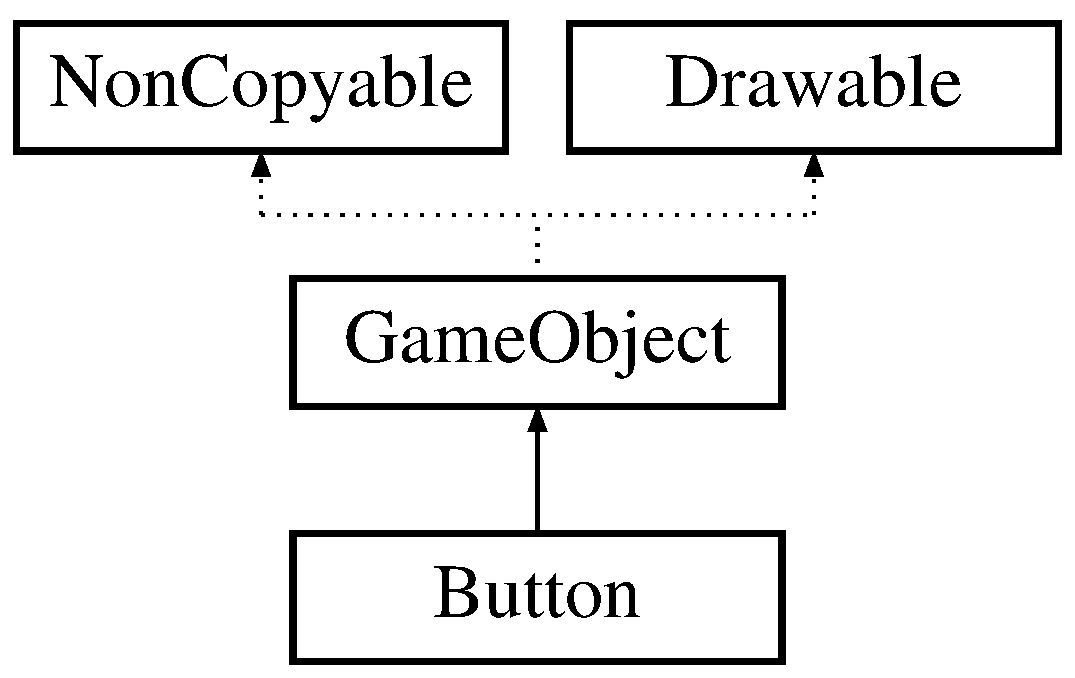
\includegraphics[height=3.000000cm]{class_button}
\end{center}
\end{figure}
\subsection*{Public Member Functions}
\begin{DoxyCompactItemize}
\item 
\hypertarget{class_button_a4ae14615e5679197f83318b743792df3}{{\bfseries Button} (const std\-::string \&name, const sf\-::\-Vector2f \&position, const sf\-::\-Vector2f \&size)}\label{class_button_a4ae14615e5679197f83318b743792df3}

\item 
\hypertarget{class_button_a53257a810c9271aecf95b1dc2c5a8883}{void {\bfseries set\-Text} (const std\-::string \&txt)}\label{class_button_a53257a810c9271aecf95b1dc2c5a8883}

\item 
\hypertarget{class_button_a276755f6e9d36892de9c15e4cde8de08}{bool {\bfseries was\-Clicked} () const }\label{class_button_a276755f6e9d36892de9c15e4cde8de08}

\end{DoxyCompactItemize}
\subsection*{Protected Member Functions}
\begin{DoxyCompactItemize}
\item 
\hypertarget{class_button_ad8e030c1c8846d43f3126047d4a3667f}{virtual void {\bfseries update} ()}\label{class_button_ad8e030c1c8846d43f3126047d4a3667f}

\item 
\hypertarget{class_button_abc179567c391f498ef7af8335975e68e}{virtual void {\bfseries draw} (sf\-::\-Render\-Target \&target, sf\-::\-Render\-States render\-States) const }\label{class_button_abc179567c391f498ef7af8335975e68e}

\end{DoxyCompactItemize}
\subsection*{Additional Inherited Members}


The documentation for this class was generated from the following files\-:\begin{DoxyCompactItemize}
\item 
include/Button.\-hpp\item 
src/Button.\-cpp\end{DoxyCompactItemize}

\hypertarget{structcallback__data}{\section{callback\-\_\-data Struct Reference}
\label{structcallback__data}\index{callback\-\_\-data@{callback\-\_\-data}}
}
\subsection*{Public Attributes}
\begin{DoxyCompactItemize}
\item 
\hypertarget{structcallback__data_abedf4296c2975d319fa40799a23f54de}{\hyperlink{structsqlite3}{sqlite3} $\ast$ {\bfseries db}}\label{structcallback__data_abedf4296c2975d319fa40799a23f54de}

\item 
\hypertarget{structcallback__data_a45c9183aaa07be9e2086d3ec6013c236}{int {\bfseries echo\-On}}\label{structcallback__data_a45c9183aaa07be9e2086d3ec6013c236}

\item 
\hypertarget{structcallback__data_ae3b40039c97de4fd46ae314b370dfc0c}{int {\bfseries stats\-On}}\label{structcallback__data_ae3b40039c97de4fd46ae314b370dfc0c}

\item 
\hypertarget{structcallback__data_a6e9b9db4da2d13ff827e91025ff7ff8e}{int {\bfseries cnt}}\label{structcallback__data_a6e9b9db4da2d13ff827e91025ff7ff8e}

\item 
\hypertarget{structcallback__data_af74435f6fa42509b6e2bf84d66baed72}{F\-I\-L\-E $\ast$ {\bfseries out}}\label{structcallback__data_af74435f6fa42509b6e2bf84d66baed72}

\item 
\hypertarget{structcallback__data_a05bf015336afef865c645653c8da5b37}{F\-I\-L\-E $\ast$ {\bfseries trace\-Out}}\label{structcallback__data_a05bf015336afef865c645653c8da5b37}

\item 
\hypertarget{structcallback__data_ac484e3009e75d7857e39f0c97bc0227f}{int {\bfseries n\-Err}}\label{structcallback__data_ac484e3009e75d7857e39f0c97bc0227f}

\item 
\hypertarget{structcallback__data_afb33755794b0fdb993069f78c2f7cbd8}{int {\bfseries mode}}\label{structcallback__data_afb33755794b0fdb993069f78c2f7cbd8}

\item 
\hypertarget{structcallback__data_adff77d840653bf454fe34bbb483f53bc}{int {\bfseries writable\-Schema}}\label{structcallback__data_adff77d840653bf454fe34bbb483f53bc}

\item 
\hypertarget{structcallback__data_a536becbd6527b94b07aa953dea4d5e23}{int {\bfseries show\-Header}}\label{structcallback__data_a536becbd6527b94b07aa953dea4d5e23}

\item 
\hypertarget{structcallback__data_af230a2bf2659515ab20cb8651521c7a3}{char $\ast$ {\bfseries z\-Dest\-Table}}\label{structcallback__data_af230a2bf2659515ab20cb8651521c7a3}

\item 
\hypertarget{structcallback__data_a86a0b78df0bcf34abebf2c3b002c4a4e}{char {\bfseries separator} \mbox{[}20\mbox{]}}\label{structcallback__data_a86a0b78df0bcf34abebf2c3b002c4a4e}

\item 
\hypertarget{structcallback__data_ab3a8931e699e39a443dfebb17f67db0f}{int {\bfseries col\-Width} \mbox{[}100\mbox{]}}\label{structcallback__data_ab3a8931e699e39a443dfebb17f67db0f}

\item 
\hypertarget{structcallback__data_a7d6ed83b0c8ea7524926669de9a13558}{int {\bfseries actual\-Width} \mbox{[}100\mbox{]}}\label{structcallback__data_a7d6ed83b0c8ea7524926669de9a13558}

\item 
\hypertarget{structcallback__data_adf5f480ac37d292d36223507efcf4e4b}{char {\bfseries nullvalue} \mbox{[}20\mbox{]}}\label{structcallback__data_adf5f480ac37d292d36223507efcf4e4b}

\item 
\hypertarget{structcallback__data_a2a9e29a6e29f1d2e2931d027e850a491}{struct \hyperlink{structprevious__mode__data}{previous\-\_\-mode\-\_\-data} {\bfseries explain\-Prev}}\label{structcallback__data_a2a9e29a6e29f1d2e2931d027e850a491}

\item 
\hypertarget{structcallback__data_aae6a31ddd572a5d68e2cfeb514ffd726}{char {\bfseries outfile} \mbox{[}F\-I\-L\-E\-N\-A\-M\-E\-\_\-\-M\-A\-X\mbox{]}}\label{structcallback__data_aae6a31ddd572a5d68e2cfeb514ffd726}

\item 
\hypertarget{structcallback__data_aa0634c06c7026cc0ed2e84995ed61a7c}{const char $\ast$ {\bfseries z\-Db\-Filename}}\label{structcallback__data_aa0634c06c7026cc0ed2e84995ed61a7c}

\item 
\hypertarget{structcallback__data_a06a1afdd74133b6ac5325a9e1f146b22}{const char $\ast$ {\bfseries z\-Vfs}}\label{structcallback__data_a06a1afdd74133b6ac5325a9e1f146b22}

\item 
\hypertarget{structcallback__data_a68cbfb5b75c7ef1d2edd7141ce59a8b1}{sqlite3\-\_\-stmt $\ast$ {\bfseries p\-Stmt}}\label{structcallback__data_a68cbfb5b75c7ef1d2edd7141ce59a8b1}

\item 
\hypertarget{structcallback__data_ab890ea205150f31f5d4bbd706f22ce39}{F\-I\-L\-E $\ast$ {\bfseries p\-Log}}\label{structcallback__data_ab890ea205150f31f5d4bbd706f22ce39}

\end{DoxyCompactItemize}


The documentation for this struct was generated from the following file\-:\begin{DoxyCompactItemize}
\item 
src/shell.\-c\end{DoxyCompactItemize}

\hypertarget{struct_cell_info}{\section{Cell\-Info Struct Reference}
\label{struct_cell_info}\index{Cell\-Info@{Cell\-Info}}
}
\subsection*{Public Attributes}
\begin{DoxyCompactItemize}
\item 
\hypertarget{struct_cell_info_a542b041b9a54a13f7c6f2fe63e7542c0}{i64 {\bfseries n\-Key}}\label{struct_cell_info_a542b041b9a54a13f7c6f2fe63e7542c0}

\item 
\hypertarget{struct_cell_info_a595ed7eeb60ea274d868f24347b7238e}{u8 $\ast$ {\bfseries p\-Cell}}\label{struct_cell_info_a595ed7eeb60ea274d868f24347b7238e}

\item 
\hypertarget{struct_cell_info_af2301ed16c35633ec6b5d7792734a4bf}{u32 {\bfseries n\-Data}}\label{struct_cell_info_af2301ed16c35633ec6b5d7792734a4bf}

\item 
\hypertarget{struct_cell_info_ac1e3c1b4216a8e778bbac82907bb1485}{u32 {\bfseries n\-Payload}}\label{struct_cell_info_ac1e3c1b4216a8e778bbac82907bb1485}

\item 
\hypertarget{struct_cell_info_a99bb1f87208f793359cf63e3d164025b}{u16 {\bfseries n\-Header}}\label{struct_cell_info_a99bb1f87208f793359cf63e3d164025b}

\item 
\hypertarget{struct_cell_info_a8cedbcc2c94916fe5798b502c614bb08}{u16 {\bfseries n\-Local}}\label{struct_cell_info_a8cedbcc2c94916fe5798b502c614bb08}

\item 
\hypertarget{struct_cell_info_af7be0161f1c67600aeba783a68972f70}{u16 {\bfseries i\-Overflow}}\label{struct_cell_info_af7be0161f1c67600aeba783a68972f70}

\item 
\hypertarget{struct_cell_info_ace78ab5eb5337b686e31b895feeb0562}{u16 {\bfseries n\-Size}}\label{struct_cell_info_ace78ab5eb5337b686e31b895feeb0562}

\end{DoxyCompactItemize}


The documentation for this struct was generated from the following file\-:\begin{DoxyCompactItemize}
\item 
src/sqlite3.\-c\end{DoxyCompactItemize}

\hypertarget{class_character}{\section{Character Class Reference}
\label{class_character}\index{Character@{Character}}
}
Inheritance diagram for Character\-:\begin{figure}[H]
\begin{center}
\leavevmode
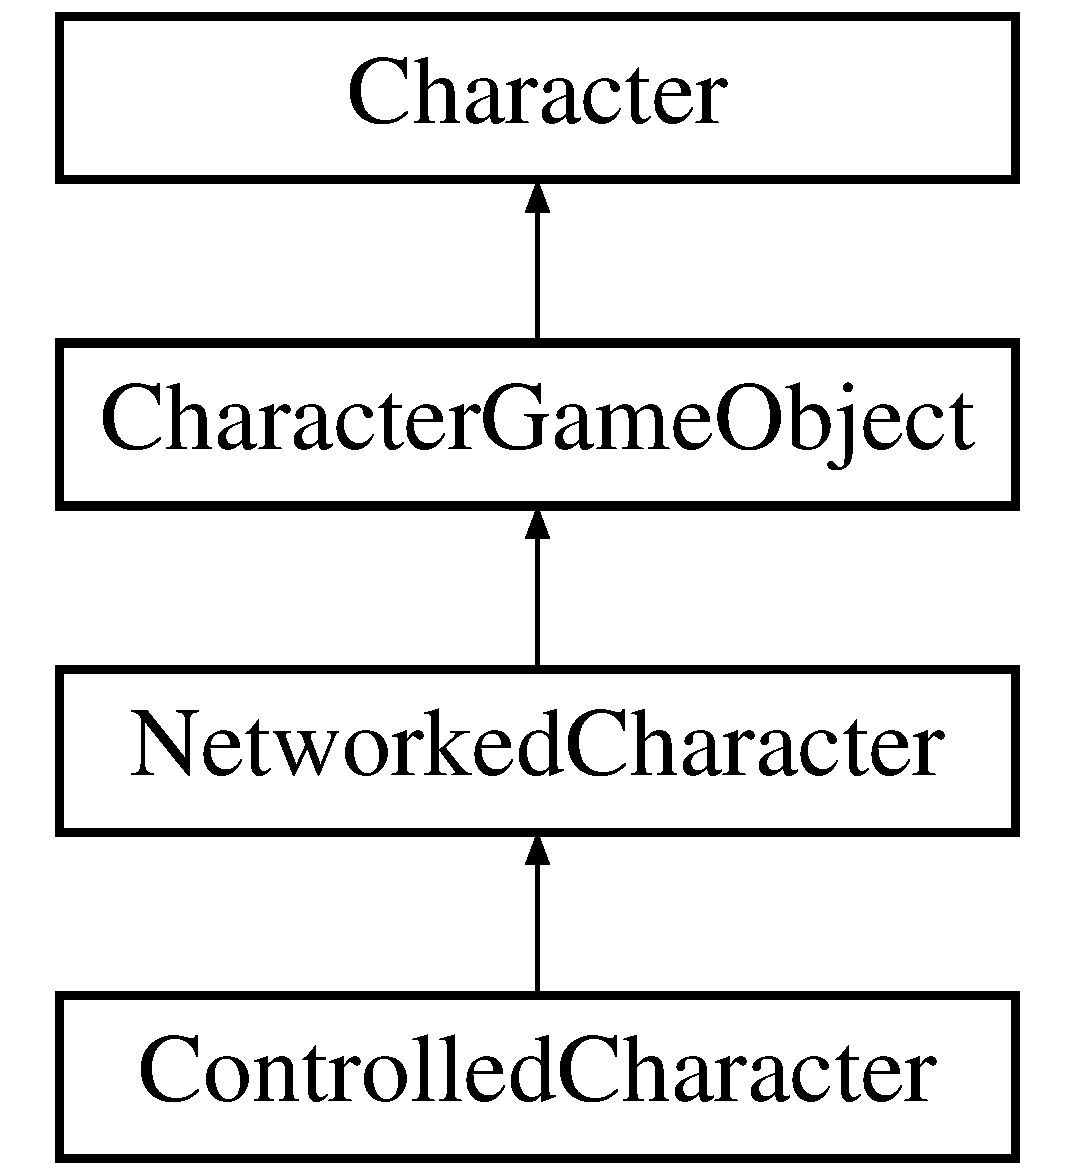
\includegraphics[height=4.000000cm]{class_character}
\end{center}
\end{figure}
\subsection*{Public Member Functions}
\begin{DoxyCompactItemize}
\item 
\hypertarget{class_character_a6eacdb4394fb452a28f11996b2802770}{void {\bfseries make\-Step} (const \hyperlink{class_key_state}{Key\-State} \&keys, float move\-Speed, float seconds)}\label{class_character_a6eacdb4394fb452a28f11996b2802770}

\item 
\hypertarget{class_character_ad48060d202444b65437a0f2b94b98db1}{glm\-::vec2 {\bfseries get\-Position} () const }\label{class_character_ad48060d202444b65437a0f2b94b98db1}

\item 
\hypertarget{class_character_aefe8c4e9a1e3aedb640fb636f6920a6c}{void {\bfseries set\-Position} (const glm\-::vec2 pos)}\label{class_character_aefe8c4e9a1e3aedb640fb636f6920a6c}

\end{DoxyCompactItemize}


The documentation for this class was generated from the following files\-:\begin{DoxyCompactItemize}
\item 
include/Character.\-hpp\item 
src/Character.\-cpp\end{DoxyCompactItemize}

\hypertarget{class_character_game_object}{\section{Character\-Game\-Object Class Reference}
\label{class_character_game_object}\index{Character\-Game\-Object@{Character\-Game\-Object}}
}
Inheritance diagram for Character\-Game\-Object\-:\begin{figure}[H]
\begin{center}
\leavevmode
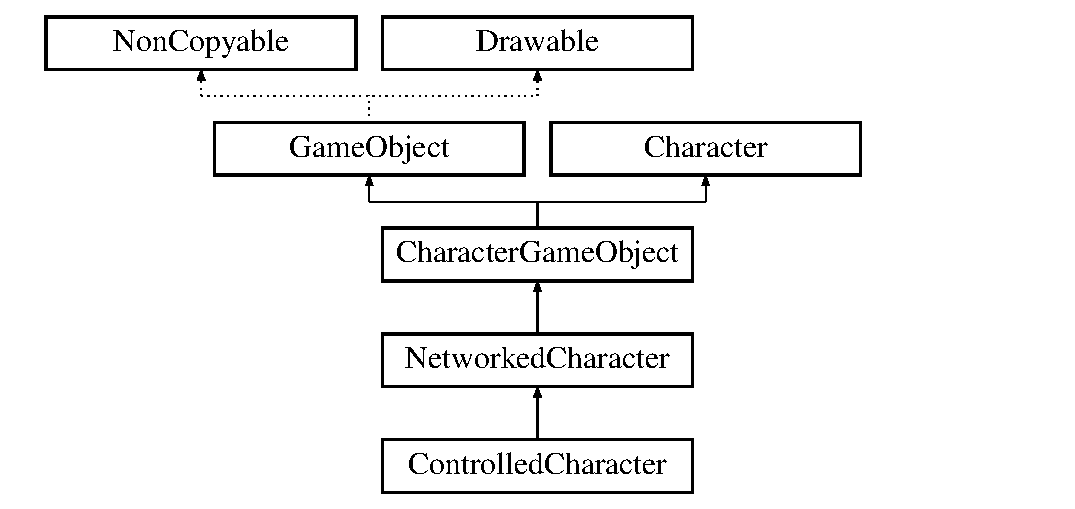
\includegraphics[height=5.000000cm]{class_character_game_object}
\end{center}
\end{figure}
\subsection*{Public Member Functions}
\begin{DoxyCompactItemize}
\item 
\hypertarget{class_character_game_object_a50d956248342bf1296fd16ba786ff0b4}{{\bfseries Character\-Game\-Object} (const std\-::string \&name, const sf\-::\-Color \&color)}\label{class_character_game_object_a50d956248342bf1296fd16ba786ff0b4}

\end{DoxyCompactItemize}
\subsection*{Protected Member Functions}
\begin{DoxyCompactItemize}
\item 
\hypertarget{class_character_game_object_a1de579718d33908a7a93a694c5b8b742}{virtual void {\bfseries update} ()}\label{class_character_game_object_a1de579718d33908a7a93a694c5b8b742}

\item 
\hypertarget{class_character_game_object_ad09908d797d148778c390a117da99be6}{virtual void {\bfseries draw} (sf\-::\-Render\-Target \&target, sf\-::\-Render\-States states) const }\label{class_character_game_object_ad09908d797d148778c390a117da99be6}

\end{DoxyCompactItemize}
\subsection*{Protected Attributes}
\begin{DoxyCompactItemize}
\item 
\hypertarget{class_character_game_object_a736ec33a6f85678d56a1885d24f6863d}{float {\bfseries player\-Move\-Speed}}\label{class_character_game_object_a736ec33a6f85678d56a1885d24f6863d}

\end{DoxyCompactItemize}
\subsection*{Additional Inherited Members}


The documentation for this class was generated from the following files\-:\begin{DoxyCompactItemize}
\item 
include/Character\-Game\-Object.\-hpp\item 
src/Character\-Game\-Object.\-cpp\end{DoxyCompactItemize}

\hypertarget{class_client}{\section{Client Class Reference}
\label{class_client}\index{Client@{Client}}
}
\subsection*{Public Member Functions}
\begin{DoxyCompactItemize}
\item 
\hypertarget{class_client_a84ca62805dedd5cfd2a064d981798ca3}{{\bfseries Client} (const std\-::string \&name, const sf\-::\-Color \&color, const sf\-::\-Ip\-Address \&ip)}\label{class_client_a84ca62805dedd5cfd2a064d981798ca3}

\end{DoxyCompactItemize}
\subsection*{Public Attributes}
\begin{DoxyCompactItemize}
\item 
\hypertarget{class_client_a989817815d95a2a9d22826c310613456}{std\-::string {\bfseries name}}\label{class_client_a989817815d95a2a9d22826c310613456}

\item 
\hypertarget{class_client_a32459cc221099ee08f9efbedff6d0202}{sf\-::\-Color {\bfseries color}}\label{class_client_a32459cc221099ee08f9efbedff6d0202}

\item 
\hypertarget{class_client_a8decfde115f9eff24b7c90b6e797a9ed}{sf\-::\-Ip\-Address {\bfseries ip}}\label{class_client_a8decfde115f9eff24b7c90b6e797a9ed}

\item 
\hypertarget{class_client_a33fcf8444e9ca2aec694c407ef1328e1}{unsigned short {\bfseries port}}\label{class_client_a33fcf8444e9ca2aec694c407ef1328e1}

\item 
\hypertarget{class_client_a03e62307136097e5e75156fd48f09bce}{\hyperlink{class_key_state}{Key\-State} {\bfseries key\-State}}\label{class_client_a03e62307136097e5e75156fd48f09bce}

\item 
\hypertarget{class_client_a3fc56e86ac001808f8a2167b98589bed}{glm\-::vec2 {\bfseries position}}\label{class_client_a3fc56e86ac001808f8a2167b98589bed}

\item 
\hypertarget{class_client_a4ad236f78ce7d19233b8b84a5fec8fb7}{float {\bfseries move\-Speed}}\label{class_client_a4ad236f78ce7d19233b8b84a5fec8fb7}

\item 
\hypertarget{class_client_a3614159a22947533499256eae1fca0b2}{int {\bfseries score}}\label{class_client_a3614159a22947533499256eae1fca0b2}

\item 
\hypertarget{class_client_afb22730fd5545399680be4df6acbd956}{\hyperlink{class_character}{Character} $\ast$ {\bfseries character}}\label{class_client_afb22730fd5545399680be4df6acbd956}

\item 
\hypertarget{class_client_a262045d2594ceedbb8bbeff5929ae982}{float {\bfseries time}}\label{class_client_a262045d2594ceedbb8bbeff5929ae982}

\item 
\hypertarget{class_client_a340d9f9680a7059fe60c7a7cdbe92969}{std\-::queue$<$ \hyperlink{class_player_state_update}{Player\-State\-Update} $>$ {\bfseries to\-Process\-Updates}}\label{class_client_a340d9f9680a7059fe60c7a7cdbe92969}

\end{DoxyCompactItemize}


The documentation for this class was generated from the following files\-:\begin{DoxyCompactItemize}
\item 
include/Client.\-hpp\item 
src/Client.\-cpp\end{DoxyCompactItemize}

\hypertarget{class_clients_manager}{\section{Clients\-Manager Class Reference}
\label{class_clients_manager}\index{Clients\-Manager@{Clients\-Manager}}
}
\subsection*{Public Types}
\begin{DoxyCompactItemize}
\item 
\hypertarget{class_clients_manager_afd5ccb0a4a115f22fc85374df568c74f}{typedef std\-::map$<$ std\-::string, \\*
\hyperlink{class_client}{Client} $\ast$ $>$ {\bfseries Clients}}\label{class_clients_manager_afd5ccb0a4a115f22fc85374df568c74f}

\end{DoxyCompactItemize}
\subsection*{Public Member Functions}
\begin{DoxyCompactItemize}
\item 
\hypertarget{class_clients_manager_af50b8efec34aa37dd60f599dda9fdc57}{{\bfseries Clients\-Manager} (bool is\-Server\-Side=false)}\label{class_clients_manager_af50b8efec34aa37dd60f599dda9fdc57}

\item 
\hypertarget{class_clients_manager_a60d59eb27425056cf2522420a1634f61}{void {\bfseries remove\-Client} (const std\-::string \&name)}\label{class_clients_manager_a60d59eb27425056cf2522420a1634f61}

\item 
\hypertarget{class_clients_manager_a0500fc808d435266e54b2b3f4640db77}{bool {\bfseries add\-Client} (const std\-::string \&name, const sf\-::\-Color \&color=sf\-::\-Color\-::\-Blue, const sf\-::\-Ip\-Address \&ip=sf\-::\-Ip\-Address\-::\-None, unsigned short port=0)}\label{class_clients_manager_a0500fc808d435266e54b2b3f4640db77}

\item 
\hypertarget{class_clients_manager_a90424f43cd357ca551625b68fa0854de}{void {\bfseries bind\-Character\-To\-Client} (std\-::string name, \hyperlink{class_networked_character}{Networked\-Character} $\ast$character)}\label{class_clients_manager_a90424f43cd357ca551625b68fa0854de}

\item 
\hypertarget{class_clients_manager_a1a3c6b502614cddb492ff1c58686e82f}{\hyperlink{class_client}{Client} $\ast$ {\bfseries get\-Client} (const std\-::string \&name)}\label{class_clients_manager_a1a3c6b502614cddb492ff1c58686e82f}

\item 
\hypertarget{class_clients_manager_a9c6bfceac0cb4fbe9bcbd367df272b50}{std\-::string {\bfseries get\-Rejection\-Reason} () const }\label{class_clients_manager_a9c6bfceac0cb4fbe9bcbd367df272b50}

\item 
void \hyperlink{class_clients_manager_ae55a1c248752d118e56da6e5a5dfa429}{extrapolate\-Positions} ()
\begin{DoxyCompactList}\small\item\em Extrapolate clients. \end{DoxyCompactList}\item 
\hypertarget{class_clients_manager_ae1bb4da6d7e6a0e5731e23811eb5dbc2}{void {\bfseries update\-Client} (const \hyperlink{class_player_state_update}{Player\-State\-Update} \&puts)}\label{class_clients_manager_ae1bb4da6d7e6a0e5731e23811eb5dbc2}

\item 
\hypertarget{class_clients_manager_a00d0c395855215143333ef4ed1187547}{Clients \& {\bfseries get\-Clients} ()}\label{class_clients_manager_a00d0c395855215143333ef4ed1187547}

\item 
\hypertarget{class_clients_manager_a8516b51b3ccb0c9b4b2583def59eece8}{sf\-::\-Packet {\bfseries get\-Client\-Updates} () const }\label{class_clients_manager_a8516b51b3ccb0c9b4b2583def59eece8}

\item 
\hypertarget{class_clients_manager_aaebc9d734a34da60dbbf17b34a5a16ac}{void {\bfseries set\-Active\-Level} (const \hyperlink{class_level}{Level} $\ast$level)}\label{class_clients_manager_aaebc9d734a34da60dbbf17b34a5a16ac}

\item 
\hypertarget{class_clients_manager_a3ef677ec0f4c253462760fb75eeb8059}{const \hyperlink{class_level}{Level} \& {\bfseries get\-Active\-Level} () const }\label{class_clients_manager_a3ef677ec0f4c253462760fb75eeb8059}

\item 
\hypertarget{class_clients_manager_ad50da4a26c76268243d717ab8c692359}{void {\bfseries reset\-Scores} ()}\label{class_clients_manager_ad50da4a26c76268243d717ab8c692359}

\item 
\hypertarget{class_clients_manager_a40bbeb61e7d3ac8b53a3cd43291de74f}{\hyperlink{class_score_change}{Score\-Change} {\bfseries get\-Scores} ()}\label{class_clients_manager_a40bbeb61e7d3ac8b53a3cd43291de74f}

\item 
\hypertarget{class_clients_manager_a35139e6bc44b908fb44ed338a10901ce}{void {\bfseries set\-Score} (const std\-::string \&name, int score)}\label{class_clients_manager_a35139e6bc44b908fb44ed338a10901ce}

\end{DoxyCompactItemize}


\subsection{Member Function Documentation}
\hypertarget{class_clients_manager_ae55a1c248752d118e56da6e5a5dfa429}{\index{Clients\-Manager@{Clients\-Manager}!extrapolate\-Positions@{extrapolate\-Positions}}
\index{extrapolate\-Positions@{extrapolate\-Positions}!ClientsManager@{Clients\-Manager}}
\subsubsection[{extrapolate\-Positions}]{\setlength{\rightskip}{0pt plus 5cm}void Clients\-Manager\-::extrapolate\-Positions (
\begin{DoxyParamCaption}
{}
\end{DoxyParamCaption}
)}}\label{class_clients_manager_ae55a1c248752d118e56da6e5a5dfa429}


Extrapolate clients. 

\begin{DoxyReturn}{Returns}
Extrapolate client position based on \-: current key state current velocity current position current acceleration time since last update 
\end{DoxyReturn}


The documentation for this class was generated from the following files\-:\begin{DoxyCompactItemize}
\item 
include/Clients\-Manager.\-hpp\item 
src/Clients\-Manager.\-cpp\end{DoxyCompactItemize}

\hypertarget{struct_coll_seq}{\section{Coll\-Seq Struct Reference}
\label{struct_coll_seq}\index{Coll\-Seq@{Coll\-Seq}}
}
\subsection*{Public Attributes}
\begin{DoxyCompactItemize}
\item 
\hypertarget{struct_coll_seq_a48d6d5f71d4f8a3ab122903464e8b4a1}{char $\ast$ {\bfseries z\-Name}}\label{struct_coll_seq_a48d6d5f71d4f8a3ab122903464e8b4a1}

\item 
\hypertarget{struct_coll_seq_add27da1a70ed6f538447e9183eeb4838}{u8 {\bfseries enc}}\label{struct_coll_seq_add27da1a70ed6f538447e9183eeb4838}

\item 
\hypertarget{struct_coll_seq_a3cee924d41e730ccec7f686eb5b6f041}{void $\ast$ {\bfseries p\-User}}\label{struct_coll_seq_a3cee924d41e730ccec7f686eb5b6f041}

\item 
\hypertarget{struct_coll_seq_a47fc6d3a01eee354332ca515a8b493ce}{int($\ast$ {\bfseries x\-Cmp} )(void $\ast$, int, const void $\ast$, int, const void $\ast$)}\label{struct_coll_seq_a47fc6d3a01eee354332ca515a8b493ce}

\item 
\hypertarget{struct_coll_seq_a1c0dd3ad98c7bb2ef517f9170134a125}{void($\ast$ {\bfseries x\-Del} )(void $\ast$)}\label{struct_coll_seq_a1c0dd3ad98c7bb2ef517f9170134a125}

\end{DoxyCompactItemize}


The documentation for this struct was generated from the following file\-:\begin{DoxyCompactItemize}
\item 
src/sqlite3.\-c\end{DoxyCompactItemize}

\hypertarget{struct_column}{\section{Column Struct Reference}
\label{struct_column}\index{Column@{Column}}
}
\subsection*{Public Attributes}
\begin{DoxyCompactItemize}
\item 
\hypertarget{struct_column_a6450a4e9fde68b3a2d79425d826eccc3}{char $\ast$ {\bfseries z\-Name}}\label{struct_column_a6450a4e9fde68b3a2d79425d826eccc3}

\item 
\hypertarget{struct_column_ac4178f302df70048235660979f84ffe4}{\hyperlink{struct_expr}{Expr} $\ast$ {\bfseries p\-Dflt}}\label{struct_column_ac4178f302df70048235660979f84ffe4}

\item 
\hypertarget{struct_column_a88d29c685783cddfbd039e5674990f4b}{char $\ast$ {\bfseries z\-Dflt}}\label{struct_column_a88d29c685783cddfbd039e5674990f4b}

\item 
\hypertarget{struct_column_aef09f43479c4bd2d07f77d340020f95f}{char $\ast$ {\bfseries z\-Type}}\label{struct_column_aef09f43479c4bd2d07f77d340020f95f}

\item 
\hypertarget{struct_column_aa95909d5c77b321258622ed28d7b96eb}{char $\ast$ {\bfseries z\-Coll}}\label{struct_column_aa95909d5c77b321258622ed28d7b96eb}

\item 
\hypertarget{struct_column_a852e9a4c1c327a64d9b051dcafda3841}{u8 {\bfseries not\-Null}}\label{struct_column_a852e9a4c1c327a64d9b051dcafda3841}

\item 
\hypertarget{struct_column_ac9d6fe31c45888cecaf3f5ad5b93bf23}{char {\bfseries affinity}}\label{struct_column_ac9d6fe31c45888cecaf3f5ad5b93bf23}

\item 
\hypertarget{struct_column_abd0c79e6f531abfb54b1296ed9a72093}{u16 {\bfseries col\-Flags}}\label{struct_column_abd0c79e6f531abfb54b1296ed9a72093}

\end{DoxyCompactItemize}


The documentation for this struct was generated from the following file\-:\begin{DoxyCompactItemize}
\item 
src/sqlite3.\-c\end{DoxyCompactItemize}

\hypertarget{class_command_handler}{\section{Command\-Handler Class Reference}
\label{class_command_handler}\index{Command\-Handler@{Command\-Handler}}
}
Inheritance diagram for Command\-Handler\-:\begin{figure}[H]
\begin{center}
\leavevmode
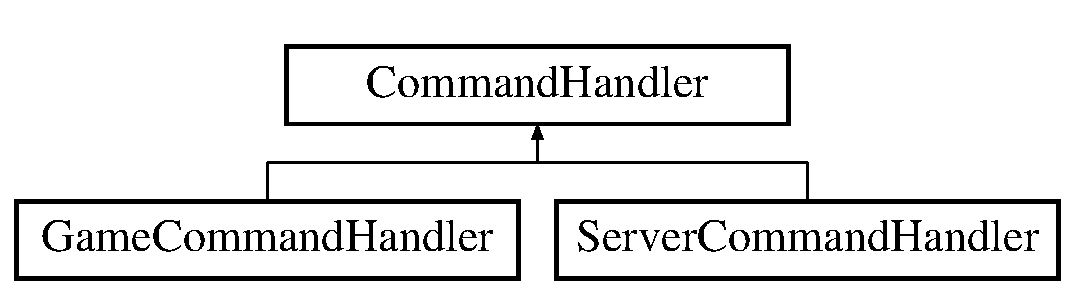
\includegraphics[height=2.000000cm]{class_command_handler}
\end{center}
\end{figure}
\subsection*{Public Member Functions}
\begin{DoxyCompactItemize}
\item 
\hypertarget{class_command_handler_a096eee4929c6cb8fa35c6c9756649d3e}{void {\bfseries handle\-Packet} (\hyperlink{struct_packet_wrap}{Packet\-Wrap} \&packwrap)}\label{class_command_handler_a096eee4929c6cb8fa35c6c9756649d3e}

\end{DoxyCompactItemize}
\subsection*{Protected Member Functions}
\begin{DoxyCompactItemize}
\item 
\hypertarget{class_command_handler_a1d0c2dc14bcc75cec3dd71724fbe4d18}{virtual void {\bfseries player\-\_\-connected} (const \hyperlink{class_player_connected}{Player\-Connected} \&pe)}\label{class_command_handler_a1d0c2dc14bcc75cec3dd71724fbe4d18}

\item 
\hypertarget{class_command_handler_a35987e69fa0f51be0bbb8e936a692943}{virtual void {\bfseries player\-\_\-authorize} (const \hyperlink{class_player_authorize}{Player\-Authorize} \&pe, const sf\-::\-Ip\-Address \&from\-Ip, unsigned short port)}\label{class_command_handler_a35987e69fa0f51be0bbb8e936a692943}

\item 
\hypertarget{class_command_handler_afc70cb365362c2cddb669adf2dbed202}{virtual void {\bfseries player\-\_\-disconnected} (const \hyperlink{class_player_disconnected}{Player\-Disconnected} \&pe)}\label{class_command_handler_afc70cb365362c2cddb669adf2dbed202}

\item 
\hypertarget{class_command_handler_a6b43e54d3fad2cb9f0313c3a7e46fc31}{virtual void {\bfseries player\-\_\-send\-\_\-message} (const \hyperlink{class_player_send_message}{Player\-Send\-Message} \&pe)}\label{class_command_handler_a6b43e54d3fad2cb9f0313c3a7e46fc31}

\item 
\hypertarget{class_command_handler_a613f3b7fefc54f7d6d3438c8220a184e}{virtual void {\bfseries player\-\_\-rejected} (const \hyperlink{class_player_rejected}{Player\-Rejected} \&pe)}\label{class_command_handler_a613f3b7fefc54f7d6d3438c8220a184e}

\item 
\hypertarget{class_command_handler_ace85a13e7d35f3895894610cb665defc}{virtual void {\bfseries player\-\_\-accepted} (const \hyperlink{class_player_accepted}{Player\-Accepted} \&pe)}\label{class_command_handler_ace85a13e7d35f3895894610cb665defc}

\item 
\hypertarget{class_command_handler_ab64f0deae690c4cdfb0f89e7f8e435ee}{virtual void {\bfseries player\-\_\-update\-\_\-to\-\_\-server} (const \hyperlink{class_player_state_update}{Player\-State\-Update} \&pe)}\label{class_command_handler_ab64f0deae690c4cdfb0f89e7f8e435ee}

\item 
\hypertarget{class_command_handler_a4038e57d46897520c478435f6b2c523a}{virtual void {\bfseries player\-\_\-update\-\_\-to\-\_\-client} (const \hyperlink{class_player_update_to_client}{Player\-Update\-To\-Client} \&pe)}\label{class_command_handler_a4038e57d46897520c478435f6b2c523a}

\item 
\hypertarget{class_command_handler_ae218cc4ddf432556c536d1199d460a08}{virtual void {\bfseries server\-\_\-entry\-\_\-get} (const \hyperlink{class_server_entry_get}{Server\-Entry\-Get} \&pe)}\label{class_command_handler_ae218cc4ddf432556c536d1199d460a08}

\item 
\hypertarget{class_command_handler_acce90c5e737c5f349f1e8e93f3e59eb2}{virtual void {\bfseries server\-\_\-entry\-\_\-add} (const \hyperlink{class_server_entry_add}{Server\-Entry\-Add} \&pe)}\label{class_command_handler_acce90c5e737c5f349f1e8e93f3e59eb2}

\item 
\hypertarget{class_command_handler_a76a5c4f33e33dea95c5cc7050f30d377}{virtual void {\bfseries server\-\_\-entry\-\_\-list} (const \hyperlink{class_server_entry_list}{Server\-Entry\-List} \&pe)}\label{class_command_handler_a76a5c4f33e33dea95c5cc7050f30d377}

\item 
\hypertarget{class_command_handler_a0d19faf20a2c40048d3faa0b5f4eca5c}{virtual void {\bfseries server\-\_\-entry\-\_\-accept} (const \hyperlink{class_server_entry_accept}{Server\-Entry\-Accept} \&pe)}\label{class_command_handler_a0d19faf20a2c40048d3faa0b5f4eca5c}

\item 
\hypertarget{class_command_handler_ad4f40da7d8732147f293f8df3b327770}{virtual void {\bfseries server\-\_\-entry\-\_\-reject} (const \hyperlink{class_server_entry_reject}{Server\-Entry\-Reject} \&pe)}\label{class_command_handler_ad4f40da7d8732147f293f8df3b327770}

\item 
\hypertarget{class_command_handler_a738593e20fa0db62aa7122384244f057}{virtual void {\bfseries load\-\_\-level} (const \hyperlink{class_load_level}{Load\-Level} \&pe)}\label{class_command_handler_a738593e20fa0db62aa7122384244f057}

\item 
\hypertarget{class_command_handler_ad43d560637d448e2280a327c79822dc1}{virtual void {\bfseries destroy\-\_\-target} (const \hyperlink{class_destroy_target}{Destroy\-Target} \&pe)}\label{class_command_handler_ad43d560637d448e2280a327c79822dc1}

\item 
\hypertarget{class_command_handler_a539b994b6264c5c286c7551580e7b5a0}{virtual void {\bfseries score\-\_\-change} (const \hyperlink{class_score_change}{Score\-Change} \&pe)}\label{class_command_handler_a539b994b6264c5c286c7551580e7b5a0}

\item 
\hypertarget{class_command_handler_a573af2e6e934d0ede953d715a92f7a43}{virtual void {\bfseries create\-\_\-target} (const \hyperlink{class_create_target}{Create\-Target} \&pe)}\label{class_command_handler_a573af2e6e934d0ede953d715a92f7a43}

\end{DoxyCompactItemize}


The documentation for this class was generated from the following files\-:\begin{DoxyCompactItemize}
\item 
include/Command\-Handler.\-hpp\item 
src/Command\-Handler.\-cpp\end{DoxyCompactItemize}

\hypertarget{structcompare_info}{\section{compare\-Info Struct Reference}
\label{structcompare_info}\index{compare\-Info@{compare\-Info}}
}
\subsection*{Public Attributes}
\begin{DoxyCompactItemize}
\item 
\hypertarget{structcompare_info_a1161e850029ef556e6daee856d32b2e2}{u8 {\bfseries match\-All}}\label{structcompare_info_a1161e850029ef556e6daee856d32b2e2}

\item 
\hypertarget{structcompare_info_ab9aabbf6d3df26bad786b532330a2fd7}{u8 {\bfseries match\-One}}\label{structcompare_info_ab9aabbf6d3df26bad786b532330a2fd7}

\item 
\hypertarget{structcompare_info_a5d2ff58a72c9eb7d22f18915c1751655}{u8 {\bfseries match\-Set}}\label{structcompare_info_a5d2ff58a72c9eb7d22f18915c1751655}

\item 
\hypertarget{structcompare_info_a6de76861b066547321f7a255cb7042ab}{u8 {\bfseries no\-Case}}\label{structcompare_info_a6de76861b066547321f7a255cb7042ab}

\end{DoxyCompactItemize}


The documentation for this struct was generated from the following file\-:\begin{DoxyCompactItemize}
\item 
src/sqlite3.\-c\end{DoxyCompactItemize}

\hypertarget{class_config_loader}{\section{Config\-Loader Class Reference}
\label{class_config_loader}\index{Config\-Loader@{Config\-Loader}}
}
Inheritance diagram for Config\-Loader\-:\begin{figure}[H]
\begin{center}
\leavevmode
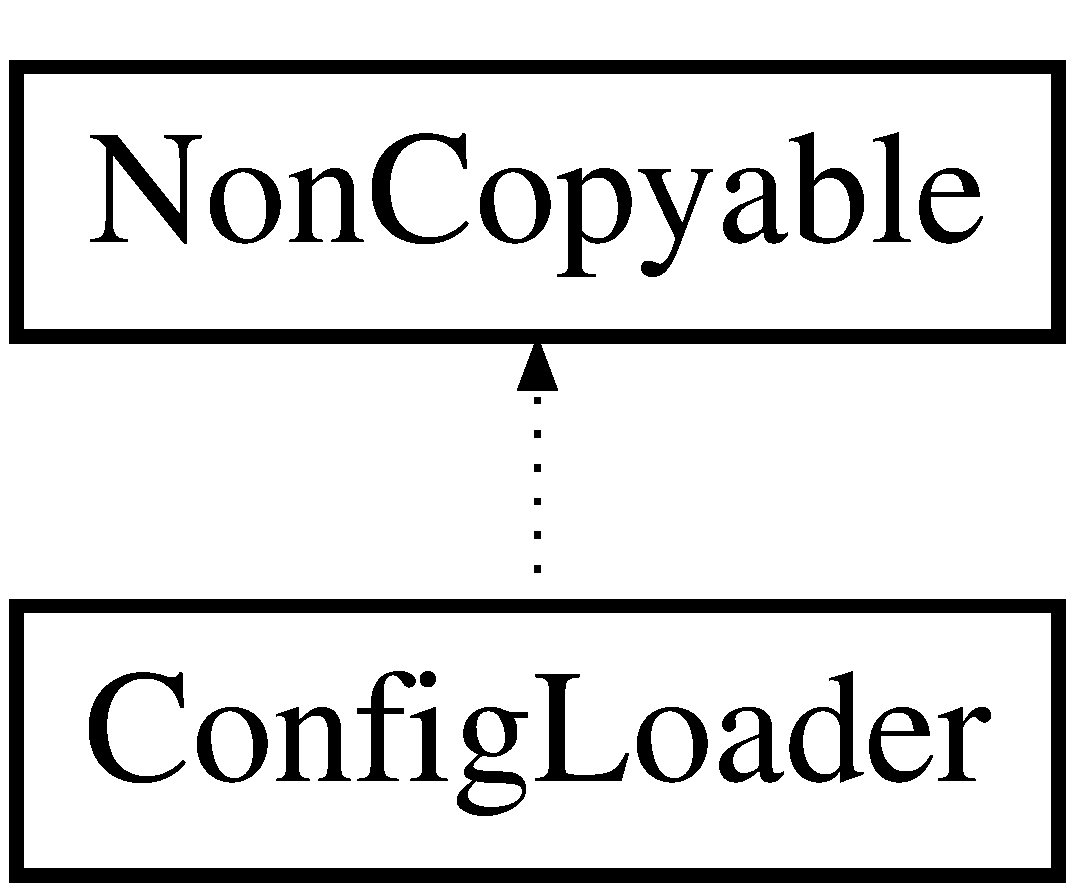
\includegraphics[height=2.000000cm]{class_config_loader}
\end{center}
\end{figure}
\subsection*{Public Member Functions}
\begin{DoxyCompactItemize}
\item 
\hypertarget{class_config_loader_addf8fb5aaf787add654ee5974a62b777}{std\-::string {\bfseries get\-Master\-Server\-Address} ()}\label{class_config_loader_addf8fb5aaf787add654ee5974a62b777}

\item 
\hypertarget{class_config_loader_ab7752bd1a81576e9321f61ff738973f9}{bool {\bfseries get\-Bool\-Setting} (std\-::string key)}\label{class_config_loader_ab7752bd1a81576e9321f61ff738973f9}

\item 
\hypertarget{class_config_loader_ac024173b366a50a19ea8a863d794f9c9}{float {\bfseries get\-Float} (std\-::string path)}\label{class_config_loader_ac024173b366a50a19ea8a863d794f9c9}

\item 
\hypertarget{class_config_loader_ad0d4ff3a501dda28bbc0927a7d6a1c51}{int {\bfseries get\-Int} (std\-::string path)}\label{class_config_loader_ad0d4ff3a501dda28bbc0927a7d6a1c51}

\item 
\hypertarget{class_config_loader_ac5196238d89cf98aae6f3c920589c7b8}{std\-::string {\bfseries get\-String} (std\-::string path)}\label{class_config_loader_ac5196238d89cf98aae6f3c920589c7b8}

\item 
\hypertarget{class_config_loader_a568d30fd1a3ab5678276992ea2336461}{std\-::vector$<$ int $>$ {\bfseries get\-Int\-Array} (std\-::string path, bool report=false)}\label{class_config_loader_a568d30fd1a3ab5678276992ea2336461}

\item 
\hypertarget{class_config_loader_a734fe8920fd3eb2312588718eb93ad72}{std\-::vector$<$ float $>$ {\bfseries get\-Float\-Array} (std\-::string path)}\label{class_config_loader_a734fe8920fd3eb2312588718eb93ad72}

\item 
\hypertarget{class_config_loader_a5fdf796fa1858924264e1206a5d427ed}{std\-::vector$<$ std\-::string $>$ {\bfseries get\-String\-Array} (std\-::string path)}\label{class_config_loader_a5fdf796fa1858924264e1206a5d427ed}

\end{DoxyCompactItemize}
\subsection*{Static Public Member Functions}
\begin{DoxyCompactItemize}
\item 
\hypertarget{class_config_loader_a24a649e36f7aac63683bfa52c2a1d1dd}{static \hyperlink{class_config_loader}{Config\-Loader} \& {\bfseries instance} ()}\label{class_config_loader_a24a649e36f7aac63683bfa52c2a1d1dd}

\end{DoxyCompactItemize}


The documentation for this class was generated from the following files\-:\begin{DoxyCompactItemize}
\item 
include/Config\-Loader.\-hpp\item 
src/Config\-Loader.\-cpp\end{DoxyCompactItemize}

\hypertarget{class_controlled_character}{\section{Controlled\-Character Class Reference}
\label{class_controlled_character}\index{Controlled\-Character@{Controlled\-Character}}
}
Inheritance diagram for Controlled\-Character\-:\begin{figure}[H]
\begin{center}
\leavevmode
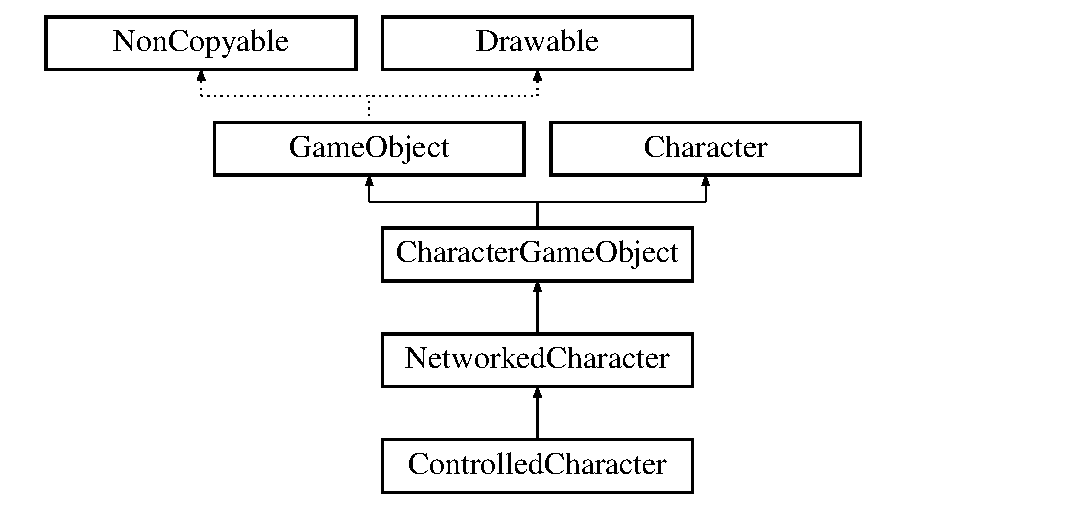
\includegraphics[height=5.000000cm]{class_controlled_character}
\end{center}
\end{figure}
\subsection*{Public Member Functions}
\begin{DoxyCompactItemize}
\item 
\hypertarget{class_controlled_character_ae1733b6dde703cf779b696671b1d6d46}{{\bfseries Controlled\-Character} (const std\-::string \&name, const sf\-::\-Color \&color)}\label{class_controlled_character_ae1733b6dde703cf779b696671b1d6d46}

\item 
\hypertarget{class_controlled_character_a234f336f78643cf9175a7b39d1582c2d}{\hyperlink{class_key_state}{Key\-State} {\bfseries get\-Key\-State} () const }\label{class_controlled_character_a234f336f78643cf9175a7b39d1582c2d}

\item 
\hypertarget{class_controlled_character_abfcca4810e477f4270a62c086a60f639}{void {\bfseries set\-Key\-State} (const \hyperlink{class_key_state}{Key\-State} \&a\-\_\-key\-State)}\label{class_controlled_character_abfcca4810e477f4270a62c086a60f639}

\end{DoxyCompactItemize}
\subsection*{Protected Member Functions}
\begin{DoxyCompactItemize}
\item 
\hypertarget{class_controlled_character_a8d7919066adeb097994fb109d554eded}{virtual void {\bfseries start} ()}\label{class_controlled_character_a8d7919066adeb097994fb109d554eded}

\item 
\hypertarget{class_controlled_character_a83d083710dde7af78186c32ace3efb0b}{virtual void {\bfseries update} ()}\label{class_controlled_character_a83d083710dde7af78186c32ace3efb0b}

\end{DoxyCompactItemize}
\subsection*{Additional Inherited Members}


The documentation for this class was generated from the following files\-:\begin{DoxyCompactItemize}
\item 
include/Controlled\-Character.\-hpp\item 
src/Controlled\-Character.\-cpp\end{DoxyCompactItemize}

\hypertarget{class_controller}{\section{Controller Class Reference}
\label{class_controller}\index{Controller@{Controller}}
}
\subsection*{Public Member Functions}
\begin{DoxyCompactItemize}
\item 
\hypertarget{class_controller_a1dd7b13f9d247cfb325a60aaff59ed13}{{\bfseries Controller} (sf\-::\-Render\-Window \&window)}\label{class_controller_a1dd7b13f9d247cfb325a60aaff59ed13}

\item 
\hypertarget{class_controller_a7d04c17913f04f99429aa29fa8505484}{void {\bfseries update} ()}\label{class_controller_a7d04c17913f04f99429aa29fa8505484}

\item 
\hypertarget{class_controller_a59f4b9e698c7d0448fde49074b1a1cce}{bool {\bfseries running} () const }\label{class_controller_a59f4b9e698c7d0448fde49074b1a1cce}

\item 
\hypertarget{class_controller_a91c1ec826fcccc82654154ac934cc332}{virtual const std\-::string {\bfseries get\-Name} ()}\label{class_controller_a91c1ec826fcccc82654154ac934cc332}

\item 
\hypertarget{class_controller_afa31ab73a5339d64c41742e7ec45759c}{void {\bfseries stop\-Running} ()}\label{class_controller_afa31ab73a5339d64c41742e7ec45759c}

\end{DoxyCompactItemize}
\subsection*{Static Public Member Functions}
\begin{DoxyCompactItemize}
\item 
\hypertarget{class_controller_acd9b2329e852e1857a7c6d3c9478cf0d}{static bool {\bfseries get\-Key} (sf\-::\-Keyboard\-::\-Key key\-Code)}\label{class_controller_acd9b2329e852e1857a7c6d3c9478cf0d}

\item 
\hypertarget{class_controller_acd28421325f54ebf707f4befd22be9ae}{static bool {\bfseries get\-Key\-Down} (sf\-::\-Keyboard\-::\-Key key\-Code)}\label{class_controller_acd28421325f54ebf707f4befd22be9ae}

\item 
\hypertarget{class_controller_a287e959445a85c875f6104ae70e86860}{static bool {\bfseries get\-Key\-Up} (sf\-::\-Keyboard\-::\-Key key\-Code)}\label{class_controller_a287e959445a85c875f6104ae70e86860}

\item 
\hypertarget{class_controller_a541c11ba7a31bdbe031e1a98b4c8d353}{static bool {\bfseries get\-Button} (sf\-::\-Mouse\-::\-Button button)}\label{class_controller_a541c11ba7a31bdbe031e1a98b4c8d353}

\item 
\hypertarget{class_controller_a198eb526541a114f2e249b6fee645624}{static bool {\bfseries get\-Button\-Down} (sf\-::\-Mouse\-::\-Button button)}\label{class_controller_a198eb526541a114f2e249b6fee645624}

\item 
\hypertarget{class_controller_a96ce3929a258e1d00a62cc85643a98fb}{static bool {\bfseries get\-Button\-Up} (sf\-::\-Mouse\-::\-Button button)}\label{class_controller_a96ce3929a258e1d00a62cc85643a98fb}

\item 
static bool \hyperlink{class_controller_ab199b67d544a200dccc71b5f73385f74}{get\-Text\-Entered} (std\-::string \&txt)
\begin{DoxyCompactList}\small\item\em If a text event has occurred in the last frame txt will be set to the captured text. \end{DoxyCompactList}\item 
\hypertarget{class_controller_ab5d78414b0896e1d62a6a95d60db4241}{static glm\-::vec2 {\bfseries get\-Delta\-Mouse} ()}\label{class_controller_ab5d78414b0896e1d62a6a95d60db4241}

\end{DoxyCompactItemize}
\subsection*{Static Public Attributes}
\begin{DoxyCompactItemize}
\item 
\hypertarget{class_controller_a478768392c69a1bef3f77e0944d3560e}{static glm\-::vec2 {\bfseries mouse\-Position}}\label{class_controller_a478768392c69a1bef3f77e0944d3560e}

\item 
\hypertarget{class_controller_aa87365fb3d3b58bfb15c9a0d43d2b0e6}{static glm\-::vec2 {\bfseries last\-Mouse\-Position}}\label{class_controller_aa87365fb3d3b58bfb15c9a0d43d2b0e6}

\end{DoxyCompactItemize}


\subsection{Member Function Documentation}
\hypertarget{class_controller_ab199b67d544a200dccc71b5f73385f74}{\index{Controller@{Controller}!get\-Text\-Entered@{get\-Text\-Entered}}
\index{get\-Text\-Entered@{get\-Text\-Entered}!Controller@{Controller}}
\subsubsection[{get\-Text\-Entered}]{\setlength{\rightskip}{0pt plus 5cm}bool Controller\-::get\-Text\-Entered (
\begin{DoxyParamCaption}
\item[{std\-::string \&}]{txt}
\end{DoxyParamCaption}
)\hspace{0.3cm}{\ttfamily [static]}}}\label{class_controller_ab199b67d544a200dccc71b5f73385f74}


If a text event has occurred in the last frame txt will be set to the captured text. 


\begin{DoxyParams}{Parameters}
{\em string} & will be set to caught characters of the last frame. \\
\hline
\end{DoxyParams}
\begin{DoxyReturn}{Returns}
If any text was entered will return true. 
\end{DoxyReturn}


The documentation for this class was generated from the following files\-:\begin{DoxyCompactItemize}
\item 
include/Controller.\-hpp\item 
src/Controller.\-cpp\end{DoxyCompactItemize}

\hypertarget{struct_count_ctx}{\section{Count\-Ctx Struct Reference}
\label{struct_count_ctx}\index{Count\-Ctx@{Count\-Ctx}}
}
\subsection*{Public Attributes}
\begin{DoxyCompactItemize}
\item 
\hypertarget{struct_count_ctx_a141c718918dbfaa183f772bfd7a516f4}{i64 {\bfseries n}}\label{struct_count_ctx_a141c718918dbfaa183f772bfd7a516f4}

\end{DoxyCompactItemize}


The documentation for this struct was generated from the following file\-:\begin{DoxyCompactItemize}
\item 
src/sqlite3.\-c\end{DoxyCompactItemize}

\hypertarget{class_create_target}{\section{Create\-Target Class Reference}
\label{class_create_target}\index{Create\-Target@{Create\-Target}}
}


Command to create one target at position for the client.  




{\ttfamily \#include $<$Network\-Events.\-h$>$}

Inheritance diagram for Create\-Target\-:\begin{figure}[H]
\begin{center}
\leavevmode
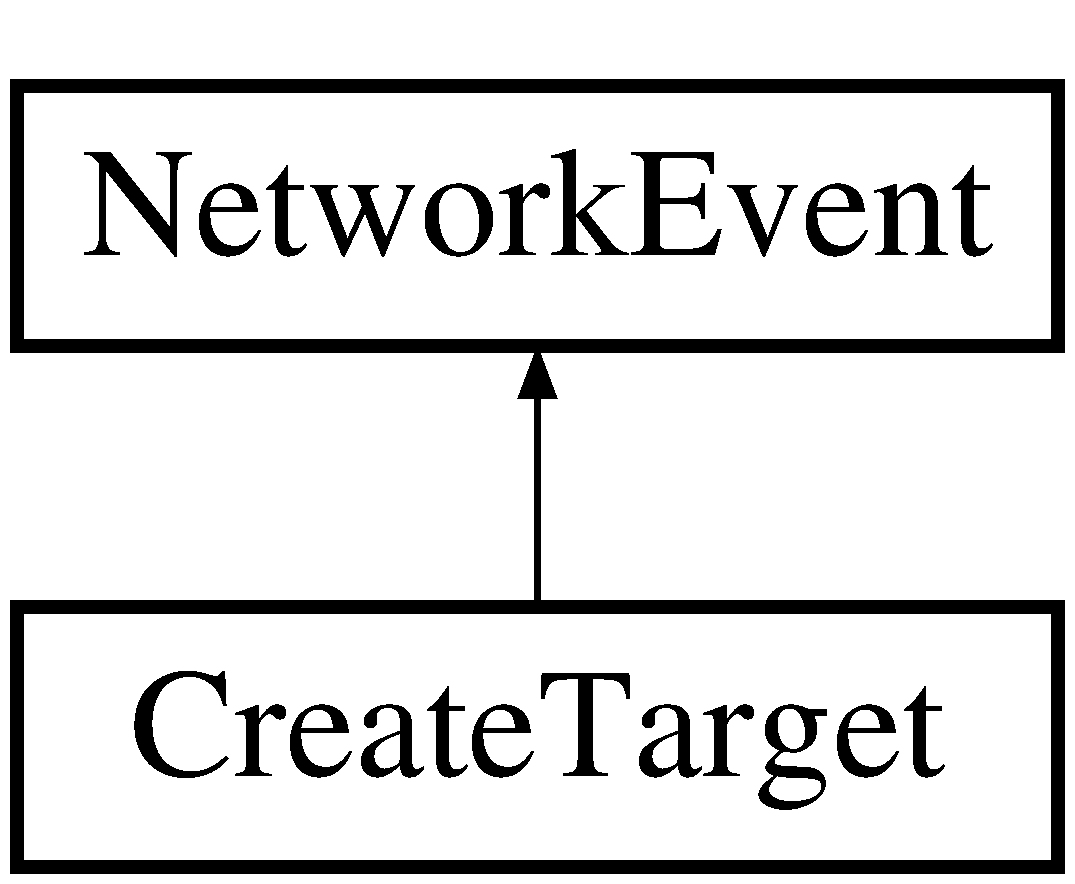
\includegraphics[height=2.000000cm]{class_create_target}
\end{center}
\end{figure}
\subsection*{Public Member Functions}
\begin{DoxyCompactItemize}
\item 
\hypertarget{class_create_target_ac23134e69bdccc45c07f3932eeef6b80}{virtual sf\-::\-Int32 {\bfseries get\-Command} () const }\label{class_create_target_ac23134e69bdccc45c07f3932eeef6b80}

\end{DoxyCompactItemize}
\subsection*{Public Attributes}
\begin{DoxyCompactItemize}
\item 
\hypertarget{class_create_target_a88833d79d83a7db0906a759fb03b10e9}{unsigned int {\bfseries target\-Id}}\label{class_create_target_a88833d79d83a7db0906a759fb03b10e9}

\item 
\hypertarget{class_create_target_a89b1d2edc2c1c1098b9d494e2aa13c98}{glm\-::vec2 {\bfseries position}}\label{class_create_target_a89b1d2edc2c1c1098b9d494e2aa13c98}

\end{DoxyCompactItemize}
\subsection*{Friends}
\begin{DoxyCompactItemize}
\item 
\hypertarget{class_create_target_a1a4d3db635e21c29e29d3e7c08c255f0}{sf\-::\-Packet \& {\bfseries operator$<$$<$} (sf\-::\-Packet \&packet, const \hyperlink{class_create_target}{Create\-Target} \&tar)}\label{class_create_target_a1a4d3db635e21c29e29d3e7c08c255f0}

\item 
\hypertarget{class_create_target_a265aabcb9cbf27ec6af2305decfd677f}{sf\-::\-Packet \& {\bfseries operator$>$$>$} (sf\-::\-Packet \&packet, \hyperlink{class_create_target}{Create\-Target} \&tar)}\label{class_create_target_a265aabcb9cbf27ec6af2305decfd677f}

\end{DoxyCompactItemize}
\subsection*{Additional Inherited Members}


\subsection{Detailed Description}
Command to create one target at position for the client. 



The documentation for this class was generated from the following file\-:\begin{DoxyCompactItemize}
\item 
include/Network\-Events.\-h\end{DoxyCompactItemize}

\hypertarget{class_database_manager}{\section{Database\-Manager Class Reference}
\label{class_database_manager}\index{Database\-Manager@{Database\-Manager}}
}
\subsection*{Public Member Functions}
\begin{DoxyCompactItemize}
\item 
bool \hyperlink{class_database_manager_a0e91c70888a0c4f79e95c31a916ad8a0}{login} (const std\-::string \&name, const std\-::string \&pw, std\-::string \&rejection\-Reason)
\begin{DoxyCompactList}\small\item\em Attempt a log in. \end{DoxyCompactList}\item 
\hypertarget{class_database_manager_af1341a35233b2e23d1fec4ce190e73d3}{bool {\bfseries register\-User} (const std\-::string \&name, const std\-::string \&pw, std\-::string \&rejection\-Reason)}\label{class_database_manager_af1341a35233b2e23d1fec4ce190e73d3}

\end{DoxyCompactItemize}


\subsection{Member Function Documentation}
\hypertarget{class_database_manager_a0e91c70888a0c4f79e95c31a916ad8a0}{\index{Database\-Manager@{Database\-Manager}!login@{login}}
\index{login@{login}!DatabaseManager@{Database\-Manager}}
\subsubsection[{login}]{\setlength{\rightskip}{0pt plus 5cm}bool Database\-Manager\-::login (
\begin{DoxyParamCaption}
\item[{const std\-::string \&}]{name, }
\item[{const std\-::string \&}]{pw, }
\item[{std\-::string \&}]{rejection\-Reason}
\end{DoxyParamCaption}
)}}\label{class_database_manager_a0e91c70888a0c4f79e95c31a916ad8a0}


Attempt a log in. 


\begin{DoxyParams}{Parameters}
{\em username} & of the player to log in \\
\hline
{\em pw} & of the player to log in \\
\hline
{\em if} & failed, reason why it has failed \\
\hline
\end{DoxyParams}
\begin{DoxyReturn}{Returns}
true is successfull, false if failed, 
\end{DoxyReturn}


The documentation for this class was generated from the following files\-:\begin{DoxyCompactItemize}
\item 
include/Database\-Manager.\-hpp\item 
src/Database\-Manager.\-cpp\end{DoxyCompactItemize}

\hypertarget{struct_date_time}{\section{Date\-Time Struct Reference}
\label{struct_date_time}\index{Date\-Time@{Date\-Time}}
}
\subsection*{Public Attributes}
\begin{DoxyCompactItemize}
\item 
\hypertarget{struct_date_time_ae5043d34fa3c3c4dc1121fec886c6f10}{sqlite3\-\_\-int64 {\bfseries i\-J\-D}}\label{struct_date_time_ae5043d34fa3c3c4dc1121fec886c6f10}

\item 
\hypertarget{struct_date_time_ad39449618b2a15128e32766a208753cf}{int {\bfseries Y}}\label{struct_date_time_ad39449618b2a15128e32766a208753cf}

\item 
\hypertarget{struct_date_time_a00e6515603bb5d7c5ce79d3a5a6438a7}{int {\bfseries M}}\label{struct_date_time_a00e6515603bb5d7c5ce79d3a5a6438a7}

\item 
\hypertarget{struct_date_time_a979ec52428a05d2f2ed827345a416fa6}{int {\bfseries D}}\label{struct_date_time_a979ec52428a05d2f2ed827345a416fa6}

\item 
\hypertarget{struct_date_time_a2146547149b65f64e07e1ac6ed8654b6}{int {\bfseries h}}\label{struct_date_time_a2146547149b65f64e07e1ac6ed8654b6}

\item 
\hypertarget{struct_date_time_ac5db527c48331a515bea3b828d1a2254}{int {\bfseries m}}\label{struct_date_time_ac5db527c48331a515bea3b828d1a2254}

\item 
\hypertarget{struct_date_time_a7f5c2e587ee18014982d85eb616f09b8}{int {\bfseries tz}}\label{struct_date_time_a7f5c2e587ee18014982d85eb616f09b8}

\item 
\hypertarget{struct_date_time_a69a803afb69b74206418bda0bc1bcaa2}{double {\bfseries s}}\label{struct_date_time_a69a803afb69b74206418bda0bc1bcaa2}

\item 
\hypertarget{struct_date_time_aaa042bec0879cd922039062433f4b26f}{char {\bfseries valid\-Y\-M\-D}}\label{struct_date_time_aaa042bec0879cd922039062433f4b26f}

\item 
\hypertarget{struct_date_time_aba26b32c6142cf6bfc09db3088b90add}{char {\bfseries valid\-H\-M\-S}}\label{struct_date_time_aba26b32c6142cf6bfc09db3088b90add}

\item 
\hypertarget{struct_date_time_a1962742892150a03dc5d302f43efbb04}{char {\bfseries valid\-J\-D}}\label{struct_date_time_a1962742892150a03dc5d302f43efbb04}

\item 
\hypertarget{struct_date_time_af3dfda2bdbb2183dc1b94f449701b81e}{char {\bfseries valid\-T\-Z}}\label{struct_date_time_af3dfda2bdbb2183dc1b94f449701b81e}

\end{DoxyCompactItemize}


The documentation for this struct was generated from the following file\-:\begin{DoxyCompactItemize}
\item 
src/sqlite3.\-c\end{DoxyCompactItemize}

\hypertarget{struct_db}{\section{Db Struct Reference}
\label{struct_db}\index{Db@{Db}}
}
\subsection*{Public Attributes}
\begin{DoxyCompactItemize}
\item 
\hypertarget{struct_db_a6df2b5d7c8fd68e92cea961d9e3b279b}{char $\ast$ {\bfseries z\-Name}}\label{struct_db_a6df2b5d7c8fd68e92cea961d9e3b279b}

\item 
\hypertarget{struct_db_a0633e5a6abfc39246d07cc6a417a5852}{\hyperlink{struct_btree}{Btree} $\ast$ {\bfseries p\-Bt}}\label{struct_db_a0633e5a6abfc39246d07cc6a417a5852}

\item 
\hypertarget{struct_db_a4c5495ebea317212f0b41aa2795a7bc9}{u8 {\bfseries in\-Trans}}\label{struct_db_a4c5495ebea317212f0b41aa2795a7bc9}

\item 
\hypertarget{struct_db_a04597a5c023d8b328193450b177ff24c}{u8 {\bfseries safety\-\_\-level}}\label{struct_db_a04597a5c023d8b328193450b177ff24c}

\item 
\hypertarget{struct_db_afd8647a83a4a7053231b92814520d6d4}{\hyperlink{struct_schema}{Schema} $\ast$ {\bfseries p\-Schema}}\label{struct_db_afd8647a83a4a7053231b92814520d6d4}

\end{DoxyCompactItemize}


The documentation for this struct was generated from the following file\-:\begin{DoxyCompactItemize}
\item 
src/sqlite3.\-c\end{DoxyCompactItemize}

\hypertarget{struct_db_fixer}{\section{Db\-Fixer Struct Reference}
\label{struct_db_fixer}\index{Db\-Fixer@{Db\-Fixer}}
}
\subsection*{Public Attributes}
\begin{DoxyCompactItemize}
\item 
\hypertarget{struct_db_fixer_ac5c9b8bca3b05a66faea11dd998bf6f6}{\hyperlink{struct_parse}{Parse} $\ast$ {\bfseries p\-Parse}}\label{struct_db_fixer_ac5c9b8bca3b05a66faea11dd998bf6f6}

\item 
\hypertarget{struct_db_fixer_a302dd5335c8a982deda5bf04bae00363}{\hyperlink{struct_schema}{Schema} $\ast$ {\bfseries p\-Schema}}\label{struct_db_fixer_a302dd5335c8a982deda5bf04bae00363}

\item 
\hypertarget{struct_db_fixer_aba91df5965a99915d9180805d02c4a7f}{const char $\ast$ {\bfseries z\-Db}}\label{struct_db_fixer_aba91df5965a99915d9180805d02c4a7f}

\item 
\hypertarget{struct_db_fixer_ae4748d9e97560b7b332527434408c2e8}{const char $\ast$ {\bfseries z\-Type}}\label{struct_db_fixer_ae4748d9e97560b7b332527434408c2e8}

\item 
\hypertarget{struct_db_fixer_aedee20e10de7337651b84656ee81b39c}{const \hyperlink{struct_token}{Token} $\ast$ {\bfseries p\-Name}}\label{struct_db_fixer_aedee20e10de7337651b84656ee81b39c}

\end{DoxyCompactItemize}


The documentation for this struct was generated from the following file\-:\begin{DoxyCompactItemize}
\item 
src/sqlite3.\-c\end{DoxyCompactItemize}

\hypertarget{class_debug}{\section{Debug Class Reference}
\label{class_debug}\index{Debug@{Debug}}
}
\subsection*{Static Public Attributes}
\begin{DoxyCompactItemize}
\item 
\hypertarget{class_debug_af06c4ace776dad3156eaa37bd386f0f8}{static bool {\bfseries V\-E\-R\-B\-O\-S\-E\-\_\-\-M\-E\-S\-S\-A\-G\-E\-S}}\label{class_debug_af06c4ace776dad3156eaa37bd386f0f8}

\item 
\hypertarget{class_debug_a5d5b459c68b28b410546379e25c91bec}{static bool {\bfseries S\-K\-I\-P\-\_\-\-I\-P}}\label{class_debug_a5d5b459c68b28b410546379e25c91bec}

\item 
\hypertarget{class_debug_ac7357fa85374be165694a32530b46f0d}{static bool {\bfseries S\-K\-I\-P\-\_\-\-P\-L\-A\-Y\-E\-R\-\_\-\-N\-A\-M\-E}}\label{class_debug_ac7357fa85374be165694a32530b46f0d}

\item 
\hypertarget{class_debug_a150b7ad4b8a768895bb356e60f31390e}{static bool {\bfseries S\-K\-I\-P\-\_\-\-P\-L\-A\-Y\-E\-R\-\_\-\-C\-O\-L\-O\-R}}\label{class_debug_a150b7ad4b8a768895bb356e60f31390e}

\item 
\hypertarget{class_debug_a3b12ed81242ef6ee0390865cb5863103}{static bool {\bfseries R\-E\-Q\-U\-I\-R\-E\-\_\-\-S\-E\-R\-V\-E\-R\-\_\-\-C\-O\-N\-N\-E\-C\-T\-I\-O\-N}}\label{class_debug_a3b12ed81242ef6ee0390865cb5863103}

\item 
\hypertarget{class_debug_a6fd4c486c8853758c1718ab77009ccd9}{static bool {\bfseries D\-I\-S\-C\-O\-V\-E\-R\-\_\-\-S\-E\-R\-V\-E\-R\-S}}\label{class_debug_a6fd4c486c8853758c1718ab77009ccd9}

\item 
\hypertarget{class_debug_a90eac41a770e6311a469e5bab925e180}{static bool {\bfseries A\-U\-T\-O\-F\-I\-L\-L\-\_\-\-L\-O\-G\-G\-I\-N}}\label{class_debug_a90eac41a770e6311a469e5bab925e180}

\end{DoxyCompactItemize}


The documentation for this class was generated from the following files\-:\begin{DoxyCompactItemize}
\item 
include/Network\-Events.\-h\item 
src/Network\-Events.\-cpp\end{DoxyCompactItemize}

\hypertarget{class_destroy_target}{\section{Destroy\-Target Class Reference}
\label{class_destroy_target}\index{Destroy\-Target@{Destroy\-Target}}
}
Inheritance diagram for Destroy\-Target\-:\begin{figure}[H]
\begin{center}
\leavevmode
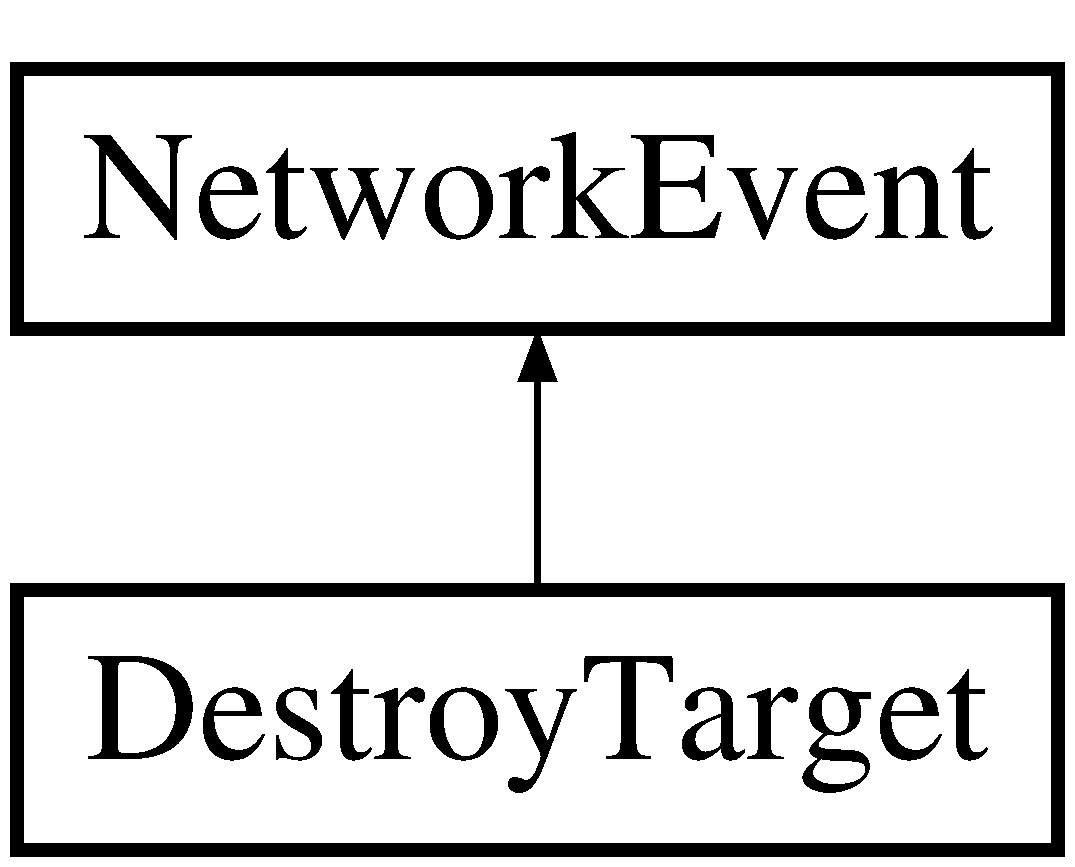
\includegraphics[height=2.000000cm]{class_destroy_target}
\end{center}
\end{figure}
\subsection*{Public Member Functions}
\begin{DoxyCompactItemize}
\item 
\hypertarget{class_destroy_target_a77ec6bb85e33331c8c4b518b859f0e84}{virtual sf\-::\-Int32 {\bfseries get\-Command} () const }\label{class_destroy_target_a77ec6bb85e33331c8c4b518b859f0e84}

\end{DoxyCompactItemize}
\subsection*{Public Attributes}
\begin{DoxyCompactItemize}
\item 
\hypertarget{class_destroy_target_ad7030853e35d7e116d1d75cecab70a0f}{unsigned int {\bfseries target\-Id}}\label{class_destroy_target_ad7030853e35d7e116d1d75cecab70a0f}

\end{DoxyCompactItemize}
\subsection*{Friends}
\begin{DoxyCompactItemize}
\item 
\hypertarget{class_destroy_target_a8e96d469a4fdf0616c50c106fe97bc66}{sf\-::\-Packet \& {\bfseries operator$<$$<$} (sf\-::\-Packet \&packet, const \hyperlink{class_destroy_target}{Destroy\-Target} \&tar)}\label{class_destroy_target_a8e96d469a4fdf0616c50c106fe97bc66}

\item 
\hypertarget{class_destroy_target_a0cf94fe4875f97e648154b9eb27adc46}{sf\-::\-Packet \& {\bfseries operator$>$$>$} (sf\-::\-Packet \&packet, \hyperlink{class_destroy_target}{Destroy\-Target} \&tar)}\label{class_destroy_target_a0cf94fe4875f97e648154b9eb27adc46}

\end{DoxyCompactItemize}
\subsection*{Additional Inherited Members}


The documentation for this class was generated from the following file\-:\begin{DoxyCompactItemize}
\item 
include/Network\-Events.\-h\end{DoxyCompactItemize}

\hypertarget{struct_distinct_ctx}{\section{Distinct\-Ctx Struct Reference}
\label{struct_distinct_ctx}\index{Distinct\-Ctx@{Distinct\-Ctx}}
}
\subsection*{Public Attributes}
\begin{DoxyCompactItemize}
\item 
\hypertarget{struct_distinct_ctx_aaaa3b23ad86358ba11b4da77cd753bbd}{u8 {\bfseries is\-Tnct}}\label{struct_distinct_ctx_aaaa3b23ad86358ba11b4da77cd753bbd}

\item 
\hypertarget{struct_distinct_ctx_ae57f819b64420f943f21d8d0e9c36205}{u8 {\bfseries e\-Tnct\-Type}}\label{struct_distinct_ctx_ae57f819b64420f943f21d8d0e9c36205}

\item 
\hypertarget{struct_distinct_ctx_af4514e425f99659e97b2bbe756716517}{int {\bfseries tab\-Tnct}}\label{struct_distinct_ctx_af4514e425f99659e97b2bbe756716517}

\item 
\hypertarget{struct_distinct_ctx_a897fdd9a1025f3d6c438a5113cf925d2}{int {\bfseries addr\-Tnct}}\label{struct_distinct_ctx_a897fdd9a1025f3d6c438a5113cf925d2}

\end{DoxyCompactItemize}


The documentation for this struct was generated from the following file\-:\begin{DoxyCompactItemize}
\item 
src/sqlite3.\-c\end{DoxyCompactItemize}

\hypertarget{structet__info}{\section{et\-\_\-info Struct Reference}
\label{structet__info}\index{et\-\_\-info@{et\-\_\-info}}
}
\subsection*{Public Attributes}
\begin{DoxyCompactItemize}
\item 
\hypertarget{structet__info_a1740af27f0c9d5840e7dda59a129aa4b}{char {\bfseries fmttype}}\label{structet__info_a1740af27f0c9d5840e7dda59a129aa4b}

\item 
\hypertarget{structet__info_a20f5a4c11c7aa1d9c777805d11965c66}{et\-Byte {\bfseries base}}\label{structet__info_a20f5a4c11c7aa1d9c777805d11965c66}

\item 
\hypertarget{structet__info_a8f11646aaec803f0870683dc3ba2f756}{et\-Byte {\bfseries flags}}\label{structet__info_a8f11646aaec803f0870683dc3ba2f756}

\item 
\hypertarget{structet__info_a148bd1efa49018c9a723701ba5747825}{et\-Byte {\bfseries type}}\label{structet__info_a148bd1efa49018c9a723701ba5747825}

\item 
\hypertarget{structet__info_a77131acb7479b0e6aad61af0901e11c2}{et\-Byte {\bfseries charset}}\label{structet__info_a77131acb7479b0e6aad61af0901e11c2}

\item 
\hypertarget{structet__info_a23cc866bf202c34e49bd49599b051628}{et\-Byte {\bfseries prefix}}\label{structet__info_a23cc866bf202c34e49bd49599b051628}

\end{DoxyCompactItemize}


The documentation for this struct was generated from the following file\-:\begin{DoxyCompactItemize}
\item 
src/sqlite3.\-c\end{DoxyCompactItemize}

\hypertarget{struct_explain}{\section{Explain Struct Reference}
\label{struct_explain}\index{Explain@{Explain}}
}
\subsection*{Public Attributes}
\begin{DoxyCompactItemize}
\item 
\hypertarget{struct_explain_a5b40aff5e9132f568c01f5790c69cc89}{\hyperlink{struct_vdbe}{Vdbe} $\ast$ {\bfseries p\-Vdbe}}\label{struct_explain_a5b40aff5e9132f568c01f5790c69cc89}

\item 
\hypertarget{struct_explain_af92c731731b19685b567d29493f1e83e}{\hyperlink{struct_str_accum}{Str\-Accum} {\bfseries str}}\label{struct_explain_af92c731731b19685b567d29493f1e83e}

\item 
\hypertarget{struct_explain_a5420e5a4c88050c6536328612fcad2b7}{int {\bfseries n\-Indent}}\label{struct_explain_a5420e5a4c88050c6536328612fcad2b7}

\item 
\hypertarget{struct_explain_ac80869acc619d982c3246134678b4d6e}{u16 {\bfseries a\-Indent} \mbox{[}100\mbox{]}}\label{struct_explain_ac80869acc619d982c3246134678b4d6e}

\item 
\hypertarget{struct_explain_a1ac782f9829311d6b85edc1707ef8d41}{char {\bfseries z\-Base} \mbox{[}100\mbox{]}}\label{struct_explain_a1ac782f9829311d6b85edc1707ef8d41}

\end{DoxyCompactItemize}


The documentation for this struct was generated from the following file\-:\begin{DoxyCompactItemize}
\item 
src/sqlite3.\-c\end{DoxyCompactItemize}

\hypertarget{struct_expr}{\section{Expr Struct Reference}
\label{struct_expr}\index{Expr@{Expr}}
}
\subsection*{Public Attributes}
\begin{DoxyCompactItemize}
\item 
\hypertarget{struct_expr_a101c55ddb6c149d95f0327831eb78225}{u8 {\bfseries op}}\label{struct_expr_a101c55ddb6c149d95f0327831eb78225}

\item 
\hypertarget{struct_expr_aeb51b76e606d6fbae234e38473bf3dc9}{char {\bfseries affinity}}\label{struct_expr_aeb51b76e606d6fbae234e38473bf3dc9}

\item 
\hypertarget{struct_expr_ad6013561807a4a5182ce928f263bc3bf}{u16 {\bfseries flags}}\label{struct_expr_ad6013561807a4a5182ce928f263bc3bf}

\item 
\hypertarget{struct_expr_aef8fabc8205ec52067df9c9b3db8588b}{\begin{tabbing}
xx\=xx\=xx\=xx\=xx\=xx\=xx\=xx\=xx\=\kill
union \{\\
\>char $\ast$ {\bfseries zToken}\\
\>int {\bfseries iValue}\\
\} {\bfseries u}}\label{struct_expr_aef8fabc8205ec52067df9c9b3db8588b}
\\

\end{tabbing}\item 
\hypertarget{struct_expr_a0a78282ae0d696f4a25013a12e38b1ba}{\hyperlink{struct_expr}{Expr} $\ast$ {\bfseries p\-Left}}\label{struct_expr_a0a78282ae0d696f4a25013a12e38b1ba}

\item 
\hypertarget{struct_expr_aa08c218d5b0b6f8882e8bf9ec8822a08}{\hyperlink{struct_expr}{Expr} $\ast$ {\bfseries p\-Right}}\label{struct_expr_aa08c218d5b0b6f8882e8bf9ec8822a08}

\item 
\hypertarget{struct_expr_a2d0647c6c3e3c69c72b73f38ec33fc2e}{\begin{tabbing}
xx\=xx\=xx\=xx\=xx\=xx\=xx\=xx\=xx\=\kill
union \{\\
\>\hyperlink{struct_expr_list}{ExprList} $\ast$ {\bfseries pList}\\
\>\hyperlink{struct_select}{Select} $\ast$ {\bfseries pSelect}\\
\} {\bfseries x}}\label{struct_expr_a2d0647c6c3e3c69c72b73f38ec33fc2e}
\\

\end{tabbing}\item 
\hypertarget{struct_expr_a5a893ea309f801f23404e7e5ac02732b}{int {\bfseries n\-Height}}\label{struct_expr_a5a893ea309f801f23404e7e5ac02732b}

\item 
\hypertarget{struct_expr_af8e273f4d7d173bfb5996ed09054611c}{int {\bfseries i\-Table}}\label{struct_expr_af8e273f4d7d173bfb5996ed09054611c}

\item 
\hypertarget{struct_expr_ad19251a8eb6db3cf0bdffe0dcb07eeba}{yn\-Var {\bfseries i\-Column}}\label{struct_expr_ad19251a8eb6db3cf0bdffe0dcb07eeba}

\item 
\hypertarget{struct_expr_a9fe0ed6360b0a4cf5b67ab8def922033}{i16 {\bfseries i\-Agg}}\label{struct_expr_a9fe0ed6360b0a4cf5b67ab8def922033}

\item 
\hypertarget{struct_expr_aa49b76f3628a7bf2b0997c33461cc651}{i16 {\bfseries i\-Right\-Join\-Table}}\label{struct_expr_aa49b76f3628a7bf2b0997c33461cc651}

\item 
\hypertarget{struct_expr_af8d40f8e74d07557e89cfffeef3657e9}{u8 {\bfseries flags2}}\label{struct_expr_af8d40f8e74d07557e89cfffeef3657e9}

\item 
\hypertarget{struct_expr_a0eacba0a2a6977e434b096b1cb9d5b9e}{u8 {\bfseries op2}}\label{struct_expr_a0eacba0a2a6977e434b096b1cb9d5b9e}

\item 
\hypertarget{struct_expr_a4fde82477256ee85f3a906263549082a}{\hyperlink{struct_agg_info}{Agg\-Info} $\ast$ {\bfseries p\-Agg\-Info}}\label{struct_expr_a4fde82477256ee85f3a906263549082a}

\item 
\hypertarget{struct_expr_a27c8824b41d853eeeebe61cf3ac1ae5a}{\hyperlink{struct_table}{Table} $\ast$ {\bfseries p\-Tab}}\label{struct_expr_a27c8824b41d853eeeebe61cf3ac1ae5a}

\end{DoxyCompactItemize}


The documentation for this struct was generated from the following file\-:\begin{DoxyCompactItemize}
\item 
src/sqlite3.\-c\end{DoxyCompactItemize}

\hypertarget{struct_expr_list}{\section{Expr\-List Struct Reference}
\label{struct_expr_list}\index{Expr\-List@{Expr\-List}}
}
\subsection*{Classes}
\begin{DoxyCompactItemize}
\item 
struct \hyperlink{struct_expr_list_1_1_expr_list__item}{Expr\-List\-\_\-item}
\end{DoxyCompactItemize}
\subsection*{Public Attributes}
\begin{DoxyCompactItemize}
\item 
\hypertarget{struct_expr_list_a88bdbd62cce306124eea63ae9f80ec33}{int {\bfseries n\-Expr}}\label{struct_expr_list_a88bdbd62cce306124eea63ae9f80ec33}

\item 
\hypertarget{struct_expr_list_aab870b9af60d25992f8672331d951ca0}{int {\bfseries i\-E\-Cursor}}\label{struct_expr_list_aab870b9af60d25992f8672331d951ca0}

\item 
\hypertarget{struct_expr_list_a02a4222d2dc4da64dcec416188abc16c}{struct \hyperlink{struct_expr_list_1_1_expr_list__item}{Expr\-List\-::\-Expr\-List\-\_\-item} $\ast$ {\bfseries a}}\label{struct_expr_list_a02a4222d2dc4da64dcec416188abc16c}

\end{DoxyCompactItemize}


The documentation for this struct was generated from the following file\-:\begin{DoxyCompactItemize}
\item 
src/sqlite3.\-c\end{DoxyCompactItemize}

\hypertarget{struct_expr_list_1_1_expr_list__item}{\section{Expr\-List\-:\-:Expr\-List\-\_\-item Struct Reference}
\label{struct_expr_list_1_1_expr_list__item}\index{Expr\-List\-::\-Expr\-List\-\_\-item@{Expr\-List\-::\-Expr\-List\-\_\-item}}
}
\subsection*{Public Attributes}
\begin{DoxyCompactItemize}
\item 
\hypertarget{struct_expr_list_1_1_expr_list__item_a75906cf3ff19e5bf16373fec7f3c79ad}{\hyperlink{struct_expr}{Expr} $\ast$ {\bfseries p\-Expr}}\label{struct_expr_list_1_1_expr_list__item_a75906cf3ff19e5bf16373fec7f3c79ad}

\item 
\hypertarget{struct_expr_list_1_1_expr_list__item_af278eb03a1169c73d144547adaf9b04f}{char $\ast$ {\bfseries z\-Name}}\label{struct_expr_list_1_1_expr_list__item_af278eb03a1169c73d144547adaf9b04f}

\item 
\hypertarget{struct_expr_list_1_1_expr_list__item_ade485bb6fafb44ec2aba59d05b8d117b}{char $\ast$ {\bfseries z\-Span}}\label{struct_expr_list_1_1_expr_list__item_ade485bb6fafb44ec2aba59d05b8d117b}

\item 
\hypertarget{struct_expr_list_1_1_expr_list__item_af9084dc073f96792c0c7a8a894778881}{u8 {\bfseries sort\-Order}}\label{struct_expr_list_1_1_expr_list__item_af9084dc073f96792c0c7a8a894778881}

\item 
\hypertarget{struct_expr_list_1_1_expr_list__item_a84aad270c98e28a725a840aac3ee8576}{u8 {\bfseries done}}\label{struct_expr_list_1_1_expr_list__item_a84aad270c98e28a725a840aac3ee8576}

\item 
\hypertarget{struct_expr_list_1_1_expr_list__item_ae1d4a3f24152d41772694bebef2ef81c}{u16 {\bfseries i\-Order\-By\-Col}}\label{struct_expr_list_1_1_expr_list__item_ae1d4a3f24152d41772694bebef2ef81c}

\item 
\hypertarget{struct_expr_list_1_1_expr_list__item_a06fc9fdfb94d35ec6ca742da23609239}{u16 {\bfseries i\-Alias}}\label{struct_expr_list_1_1_expr_list__item_a06fc9fdfb94d35ec6ca742da23609239}

\end{DoxyCompactItemize}


The documentation for this struct was generated from the following file\-:\begin{DoxyCompactItemize}
\item 
src/sqlite3.\-c\end{DoxyCompactItemize}

\hypertarget{struct_expr_span}{\section{Expr\-Span Struct Reference}
\label{struct_expr_span}\index{Expr\-Span@{Expr\-Span}}
}
\subsection*{Public Attributes}
\begin{DoxyCompactItemize}
\item 
\hypertarget{struct_expr_span_a081c4aa031331c8518c1173b2a8335cc}{\hyperlink{struct_expr}{Expr} $\ast$ {\bfseries p\-Expr}}\label{struct_expr_span_a081c4aa031331c8518c1173b2a8335cc}

\item 
\hypertarget{struct_expr_span_af4653638d7e67a62e7a607f682b38e25}{const char $\ast$ {\bfseries z\-Start}}\label{struct_expr_span_af4653638d7e67a62e7a607f682b38e25}

\item 
\hypertarget{struct_expr_span_a7cdf42cea729fcb5a1c477c3825ab575}{const char $\ast$ {\bfseries z\-End}}\label{struct_expr_span_a7cdf42cea729fcb5a1c477c3825ab575}

\end{DoxyCompactItemize}


The documentation for this struct was generated from the following file\-:\begin{DoxyCompactItemize}
\item 
src/sqlite3.\-c\end{DoxyCompactItemize}

\hypertarget{class_json_1_1_fast_writer}{\section{Json\-:\-:Fast\-Writer Class Reference}
\label{class_json_1_1_fast_writer}\index{Json\-::\-Fast\-Writer@{Json\-::\-Fast\-Writer}}
}


Outputs a \hyperlink{class_json_1_1_value}{Value} in \href{http://www.json.org}{\tt J\-S\-O\-N} format without formatting (not human friendly).  




{\ttfamily \#include $<$json.\-h$>$}

Inheritance diagram for Json\-:\-:Fast\-Writer\-:\begin{figure}[H]
\begin{center}
\leavevmode
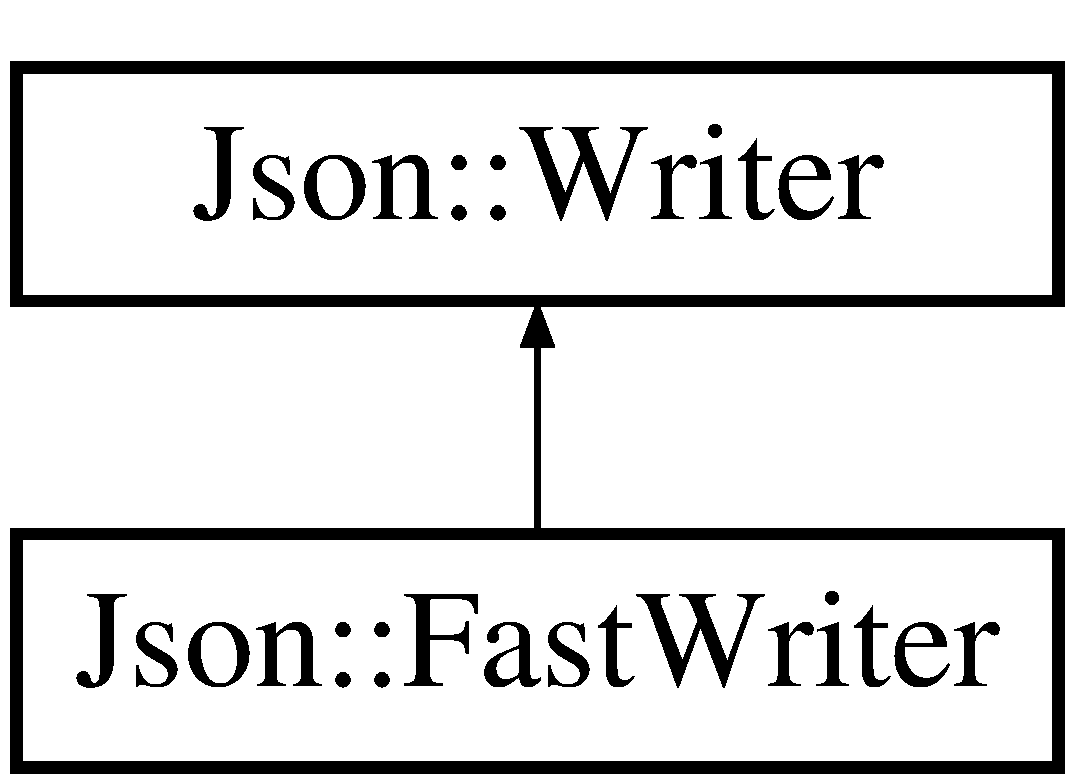
\includegraphics[height=2.000000cm]{class_json_1_1_fast_writer}
\end{center}
\end{figure}
\subsection*{Public Member Functions}
\begin{DoxyCompactItemize}
\item 
\hypertarget{class_json_1_1_fast_writer_a78d98e9f76d33660ad6e6a1abe287d45}{void {\bfseries enable\-Y\-A\-M\-L\-Compatibility} ()}\label{class_json_1_1_fast_writer_a78d98e9f76d33660ad6e6a1abe287d45}

\item 
\hypertarget{class_json_1_1_fast_writer_aa66218a56447222f91d64db618935a19}{virtual std\-::string {\bfseries write} (const \hyperlink{class_json_1_1_value}{Value} \&root)}\label{class_json_1_1_fast_writer_aa66218a56447222f91d64db618935a19}

\end{DoxyCompactItemize}


\subsection{Detailed Description}
Outputs a \hyperlink{class_json_1_1_value}{Value} in \href{http://www.json.org}{\tt J\-S\-O\-N} format without formatting (not human friendly). 

The J\-S\-O\-N document is written in a single line. It is not intended for 'human' consumption, but may be usefull to support feature such as R\-P\-C where bandwith is limited. \begin{DoxySeeAlso}{See Also}
\hyperlink{class_json_1_1_reader}{Reader}, \hyperlink{class_json_1_1_value}{Value} 
\end{DoxySeeAlso}


The documentation for this class was generated from the following files\-:\begin{DoxyCompactItemize}
\item 
include/json/json.\-h\item 
src/jsoncpp.\-cpp\end{DoxyCompactItemize}

\hypertarget{class_json_1_1_features}{\section{Json\-:\-:Features Class Reference}
\label{class_json_1_1_features}\index{Json\-::\-Features@{Json\-::\-Features}}
}


Configuration passed to reader and writer. This configuration object can be used to force the \hyperlink{class_json_1_1_reader}{Reader} or \hyperlink{class_json_1_1_writer}{Writer} to behave in a standard conforming way.  




{\ttfamily \#include $<$json.\-h$>$}

\subsection*{Public Member Functions}
\begin{DoxyCompactItemize}
\item 
\hypertarget{class_json_1_1_features_ad15a091cb61bb31323299a95970d2644}{\hyperlink{class_json_1_1_features_ad15a091cb61bb31323299a95970d2644}{Features} ()}\label{class_json_1_1_features_ad15a091cb61bb31323299a95970d2644}

\begin{DoxyCompactList}\small\item\em Initialize the configuration like Json\-Config\-::all\-Features;. \end{DoxyCompactList}\end{DoxyCompactItemize}
\subsection*{Static Public Member Functions}
\begin{DoxyCompactItemize}
\item 
static \hyperlink{class_json_1_1_features}{Features} \hyperlink{class_json_1_1_features_a63894da6e2c100b38741fa933f3d33ae}{all} ()
\begin{DoxyCompactList}\small\item\em A configuration that allows all features and assumes all strings are U\-T\-F-\/8. \end{DoxyCompactList}\item 
static \hyperlink{class_json_1_1_features}{Features} \hyperlink{class_json_1_1_features_ae23176c14b2e79e81fb61fb1a8ab58ee}{strict\-Mode} ()
\begin{DoxyCompactList}\small\item\em A configuration that is strictly compatible with the J\-S\-O\-N specification. \end{DoxyCompactList}\end{DoxyCompactItemize}
\subsection*{Public Attributes}
\begin{DoxyCompactItemize}
\item 
\hypertarget{class_json_1_1_features_a33afd389719624b6bdb23950b3c346c9}{bool \hyperlink{class_json_1_1_features_a33afd389719624b6bdb23950b3c346c9}{allow\-Comments\-\_\-}}\label{class_json_1_1_features_a33afd389719624b6bdb23950b3c346c9}

\begin{DoxyCompactList}\small\item\em {\ttfamily true} if comments are allowed. Default\-: {\ttfamily true}. \end{DoxyCompactList}\item 
\hypertarget{class_json_1_1_features_a1162c37a1458adc32582b585b552f9c3}{bool \hyperlink{class_json_1_1_features_a1162c37a1458adc32582b585b552f9c3}{strict\-Root\-\_\-}}\label{class_json_1_1_features_a1162c37a1458adc32582b585b552f9c3}

\begin{DoxyCompactList}\small\item\em {\ttfamily true} if root must be either an array or an object value. Default\-: {\ttfamily false}. \end{DoxyCompactList}\end{DoxyCompactItemize}


\subsection{Detailed Description}
Configuration passed to reader and writer. This configuration object can be used to force the \hyperlink{class_json_1_1_reader}{Reader} or \hyperlink{class_json_1_1_writer}{Writer} to behave in a standard conforming way. 

\subsection{Member Function Documentation}
\hypertarget{class_json_1_1_features_a63894da6e2c100b38741fa933f3d33ae}{\index{Json\-::\-Features@{Json\-::\-Features}!all@{all}}
\index{all@{all}!Json::Features@{Json\-::\-Features}}
\subsubsection[{all}]{\setlength{\rightskip}{0pt plus 5cm}{\bf Features} Json\-::\-Features\-::all (
\begin{DoxyParamCaption}
{}
\end{DoxyParamCaption}
)\hspace{0.3cm}{\ttfamily [static]}}}\label{class_json_1_1_features_a63894da6e2c100b38741fa933f3d33ae}


A configuration that allows all features and assumes all strings are U\-T\-F-\/8. 


\begin{DoxyItemize}
\item C \& C++ comments are allowed
\item Root object can be any J\-S\-O\-N value
\item Assumes \hyperlink{class_json_1_1_value}{Value} strings are encoded in U\-T\-F-\/8 
\end{DoxyItemize}\hypertarget{class_json_1_1_features_ae23176c14b2e79e81fb61fb1a8ab58ee}{\index{Json\-::\-Features@{Json\-::\-Features}!strict\-Mode@{strict\-Mode}}
\index{strict\-Mode@{strict\-Mode}!Json::Features@{Json\-::\-Features}}
\subsubsection[{strict\-Mode}]{\setlength{\rightskip}{0pt plus 5cm}{\bf Features} Json\-::\-Features\-::strict\-Mode (
\begin{DoxyParamCaption}
{}
\end{DoxyParamCaption}
)\hspace{0.3cm}{\ttfamily [static]}}}\label{class_json_1_1_features_ae23176c14b2e79e81fb61fb1a8ab58ee}


A configuration that is strictly compatible with the J\-S\-O\-N specification. 


\begin{DoxyItemize}
\item Comments are forbidden.
\item Root object must be either an array or an object value.
\item Assumes \hyperlink{class_json_1_1_value}{Value} strings are encoded in U\-T\-F-\/8 
\end{DoxyItemize}

The documentation for this class was generated from the following files\-:\begin{DoxyCompactItemize}
\item 
include/json/json.\-h\item 
src/jsoncpp.\-cpp\end{DoxyCompactItemize}

\hypertarget{struct_file_chunk}{\section{File\-Chunk Struct Reference}
\label{struct_file_chunk}\index{File\-Chunk@{File\-Chunk}}
}
\subsection*{Public Attributes}
\begin{DoxyCompactItemize}
\item 
\hypertarget{struct_file_chunk_ad2d0d170afc7ce1e239e8716852e247b}{\hyperlink{struct_file_chunk}{File\-Chunk} $\ast$ {\bfseries p\-Next}}\label{struct_file_chunk_ad2d0d170afc7ce1e239e8716852e247b}

\item 
\hypertarget{struct_file_chunk_ada06a9958ee6b82a6c2b15c29f847d19}{u8 {\bfseries z\-Chunk} \mbox{[}J\-O\-U\-R\-N\-A\-L\-\_\-\-C\-H\-U\-N\-K\-S\-I\-Z\-E\mbox{]}}\label{struct_file_chunk_ada06a9958ee6b82a6c2b15c29f847d19}

\end{DoxyCompactItemize}


The documentation for this struct was generated from the following file\-:\begin{DoxyCompactItemize}
\item 
src/sqlite3.\-c\end{DoxyCompactItemize}

\hypertarget{struct_file_point}{\section{File\-Point Struct Reference}
\label{struct_file_point}\index{File\-Point@{File\-Point}}
}
\subsection*{Public Attributes}
\begin{DoxyCompactItemize}
\item 
\hypertarget{struct_file_point_a00a345e479cd37ebeb9e6ed475eb4112}{sqlite3\-\_\-int64 {\bfseries i\-Offset}}\label{struct_file_point_a00a345e479cd37ebeb9e6ed475eb4112}

\item 
\hypertarget{struct_file_point_aa17216d9d2559f14a00a2c72a8959298}{\hyperlink{struct_file_chunk}{File\-Chunk} $\ast$ {\bfseries p\-Chunk}}\label{struct_file_point_aa17216d9d2559f14a00a2c72a8959298}

\end{DoxyCompactItemize}


The documentation for this struct was generated from the following file\-:\begin{DoxyCompactItemize}
\item 
src/sqlite3.\-c\end{DoxyCompactItemize}

\hypertarget{struct_file_writer}{\section{File\-Writer Struct Reference}
\label{struct_file_writer}\index{File\-Writer@{File\-Writer}}
}
\subsection*{Public Attributes}
\begin{DoxyCompactItemize}
\item 
\hypertarget{struct_file_writer_a9d6206477bbbd0ce69087c7f9946813d}{int {\bfseries e\-F\-W\-Err}}\label{struct_file_writer_a9d6206477bbbd0ce69087c7f9946813d}

\item 
\hypertarget{struct_file_writer_a0b1f871754a66f029bb91e497dcc7b73}{u8 $\ast$ {\bfseries a\-Buffer}}\label{struct_file_writer_a0b1f871754a66f029bb91e497dcc7b73}

\item 
\hypertarget{struct_file_writer_af2dceb2795ba9edef0158601922448e3}{int {\bfseries n\-Buffer}}\label{struct_file_writer_af2dceb2795ba9edef0158601922448e3}

\item 
\hypertarget{struct_file_writer_a64ce30042d13eeb585998f5648a6a5a8}{int {\bfseries i\-Buf\-Start}}\label{struct_file_writer_a64ce30042d13eeb585998f5648a6a5a8}

\item 
\hypertarget{struct_file_writer_ad38aa3b0a138de0c419f72c0c8994375}{int {\bfseries i\-Buf\-End}}\label{struct_file_writer_ad38aa3b0a138de0c419f72c0c8994375}

\item 
\hypertarget{struct_file_writer_ade3665625c8607582daa7130d7a2683f}{i64 {\bfseries i\-Write\-Off}}\label{struct_file_writer_ade3665625c8607582daa7130d7a2683f}

\item 
\hypertarget{struct_file_writer_a24a75f5d5d088a809c1e811154912e33}{\hyperlink{structsqlite3__file}{sqlite3\-\_\-file} $\ast$ {\bfseries p\-File}}\label{struct_file_writer_a24a75f5d5d088a809c1e811154912e33}

\end{DoxyCompactItemize}


The documentation for this struct was generated from the following file\-:\begin{DoxyCompactItemize}
\item 
src/sqlite3.\-c\end{DoxyCompactItemize}

\hypertarget{struct_f_key}{\section{F\-Key Struct Reference}
\label{struct_f_key}\index{F\-Key@{F\-Key}}
}
\subsection*{Classes}
\begin{DoxyCompactItemize}
\item 
struct \hyperlink{struct_f_key_1_1s_col_map}{s\-Col\-Map}
\end{DoxyCompactItemize}
\subsection*{Public Attributes}
\begin{DoxyCompactItemize}
\item 
\hypertarget{struct_f_key_a6d476f3fbfa75a19c5c5a9edec4e79eb}{\hyperlink{struct_table}{Table} $\ast$ {\bfseries p\-From}}\label{struct_f_key_a6d476f3fbfa75a19c5c5a9edec4e79eb}

\item 
\hypertarget{struct_f_key_ac64ff66b30167715c8822a74c2809075}{\hyperlink{struct_f_key}{F\-Key} $\ast$ {\bfseries p\-Next\-From}}\label{struct_f_key_ac64ff66b30167715c8822a74c2809075}

\item 
\hypertarget{struct_f_key_a1eac10bab38a0ac9f88306fbbabbe5d6}{char $\ast$ {\bfseries z\-To}}\label{struct_f_key_a1eac10bab38a0ac9f88306fbbabbe5d6}

\item 
\hypertarget{struct_f_key_ac29b26999113602e7e3921bf07643c04}{\hyperlink{struct_f_key}{F\-Key} $\ast$ {\bfseries p\-Next\-To}}\label{struct_f_key_ac29b26999113602e7e3921bf07643c04}

\item 
\hypertarget{struct_f_key_a56189e420e91df86513e6895db518eca}{\hyperlink{struct_f_key}{F\-Key} $\ast$ {\bfseries p\-Prev\-To}}\label{struct_f_key_a56189e420e91df86513e6895db518eca}

\item 
\hypertarget{struct_f_key_a611e3223f3f434e0a635e036dc100cbb}{int {\bfseries n\-Col}}\label{struct_f_key_a611e3223f3f434e0a635e036dc100cbb}

\item 
\hypertarget{struct_f_key_ab742714b17f2c13353837e1fdde51cc7}{u8 {\bfseries is\-Deferred}}\label{struct_f_key_ab742714b17f2c13353837e1fdde51cc7}

\item 
\hypertarget{struct_f_key_a68a08f58294bf845e9c77d785499d222}{u8 {\bfseries a\-Action} \mbox{[}2\mbox{]}}\label{struct_f_key_a68a08f58294bf845e9c77d785499d222}

\item 
\hypertarget{struct_f_key_a9ce15cb27b675836bc714ab18fd8a008}{\hyperlink{struct_trigger}{Trigger} $\ast$ {\bfseries ap\-Trigger} \mbox{[}2\mbox{]}}\label{struct_f_key_a9ce15cb27b675836bc714ab18fd8a008}

\item 
\hypertarget{struct_f_key_a5b230bc6c10a67f432ed7d5ebc92bcd2}{struct \hyperlink{struct_f_key_1_1s_col_map}{F\-Key\-::s\-Col\-Map} {\bfseries a\-Col} \mbox{[}1\mbox{]}}\label{struct_f_key_a5b230bc6c10a67f432ed7d5ebc92bcd2}

\end{DoxyCompactItemize}


The documentation for this struct was generated from the following file\-:\begin{DoxyCompactItemize}
\item 
src/sqlite3.\-c\end{DoxyCompactItemize}

\hypertarget{class_full_expression_accumulator}{\section{Full\-Expression\-Accumulator Class Reference}
\label{class_full_expression_accumulator}\index{Full\-Expression\-Accumulator@{Full\-Expression\-Accumulator}}
}
\subsection*{Public Member Functions}
\begin{DoxyCompactItemize}
\item 
\hypertarget{class_full_expression_accumulator_aa787e42e74595b276bcdb7f5787ddf99}{{\bfseries Full\-Expression\-Accumulator} (std\-::ostream \&os)}\label{class_full_expression_accumulator_aa787e42e74595b276bcdb7f5787ddf99}

\item 
\hypertarget{class_full_expression_accumulator_adf47b8e628e412f0364fab4da31cc7db}{{\footnotesize template$<$typename T $>$ }\\\hyperlink{class_full_expression_accumulator}{Full\-Expression\-Accumulator} \& {\bfseries operator$<$$<$} (T const \&t)}\label{class_full_expression_accumulator_adf47b8e628e412f0364fab4da31cc7db}

\end{DoxyCompactItemize}


The documentation for this class was generated from the following file\-:\begin{DoxyCompactItemize}
\item 
include/Full\-Expression\-Accumulator.\-hpp\end{DoxyCompactItemize}

\hypertarget{struct_func_def}{\section{Func\-Def Struct Reference}
\label{struct_func_def}\index{Func\-Def@{Func\-Def}}
}
\subsection*{Public Attributes}
\begin{DoxyCompactItemize}
\item 
\hypertarget{struct_func_def_a4ad90c05868ec8ee60c211b6e20299df}{i16 {\bfseries n\-Arg}}\label{struct_func_def_a4ad90c05868ec8ee60c211b6e20299df}

\item 
\hypertarget{struct_func_def_aa7ed0a0a7d8790a4946ef0dbf85a601c}{u8 {\bfseries i\-Pref\-Enc}}\label{struct_func_def_aa7ed0a0a7d8790a4946ef0dbf85a601c}

\item 
\hypertarget{struct_func_def_aed4dc88e58b7582668bcaf425c4d053f}{u8 {\bfseries flags}}\label{struct_func_def_aed4dc88e58b7582668bcaf425c4d053f}

\item 
\hypertarget{struct_func_def_a04fdde2f96be198823a483bebcfd3ae3}{void $\ast$ {\bfseries p\-User\-Data}}\label{struct_func_def_a04fdde2f96be198823a483bebcfd3ae3}

\item 
\hypertarget{struct_func_def_a1ebe547d000172d9ae44d12eeb433a48}{\hyperlink{struct_func_def}{Func\-Def} $\ast$ {\bfseries p\-Next}}\label{struct_func_def_a1ebe547d000172d9ae44d12eeb433a48}

\item 
\hypertarget{struct_func_def_a1cfd07fdfe22ff504ea7f36c0752c1da}{void($\ast$ {\bfseries x\-Func} )(\hyperlink{structsqlite3__context}{sqlite3\-\_\-context} $\ast$, int, \hyperlink{struct_mem}{sqlite3\-\_\-value} $\ast$$\ast$)}\label{struct_func_def_a1cfd07fdfe22ff504ea7f36c0752c1da}

\item 
\hypertarget{struct_func_def_ab1d1c623844534b17ea3ccce3f815464}{void($\ast$ {\bfseries x\-Step} )(\hyperlink{structsqlite3__context}{sqlite3\-\_\-context} $\ast$, int, \hyperlink{struct_mem}{sqlite3\-\_\-value} $\ast$$\ast$)}\label{struct_func_def_ab1d1c623844534b17ea3ccce3f815464}

\item 
\hypertarget{struct_func_def_a3c649453d5a58c697b7ee54ee999e7ef}{void($\ast$ {\bfseries x\-Finalize} )(\hyperlink{structsqlite3__context}{sqlite3\-\_\-context} $\ast$)}\label{struct_func_def_a3c649453d5a58c697b7ee54ee999e7ef}

\item 
\hypertarget{struct_func_def_a1135e622a3a505c7c463e975846ef926}{char $\ast$ {\bfseries z\-Name}}\label{struct_func_def_a1135e622a3a505c7c463e975846ef926}

\item 
\hypertarget{struct_func_def_a04561444155a6922d6a2d99a29d35281}{\hyperlink{struct_func_def}{Func\-Def} $\ast$ {\bfseries p\-Hash}}\label{struct_func_def_a04561444155a6922d6a2d99a29d35281}

\item 
\hypertarget{struct_func_def_a1bd12675375b838b5c00b1c79c1e6301}{\hyperlink{struct_func_destructor}{Func\-Destructor} $\ast$ {\bfseries p\-Destructor}}\label{struct_func_def_a1bd12675375b838b5c00b1c79c1e6301}

\end{DoxyCompactItemize}


The documentation for this struct was generated from the following file\-:\begin{DoxyCompactItemize}
\item 
src/sqlite3.\-c\end{DoxyCompactItemize}

\hypertarget{struct_func_def_hash}{\section{Func\-Def\-Hash Struct Reference}
\label{struct_func_def_hash}\index{Func\-Def\-Hash@{Func\-Def\-Hash}}
}
\subsection*{Public Attributes}
\begin{DoxyCompactItemize}
\item 
\hypertarget{struct_func_def_hash_a3e044ccfe432770ef7297e86e405cc96}{\hyperlink{struct_func_def}{Func\-Def} $\ast$ {\bfseries a} \mbox{[}23\mbox{]}}\label{struct_func_def_hash_a3e044ccfe432770ef7297e86e405cc96}

\end{DoxyCompactItemize}


The documentation for this struct was generated from the following file\-:\begin{DoxyCompactItemize}
\item 
src/sqlite3.\-c\end{DoxyCompactItemize}

\hypertarget{struct_func_destructor}{\section{Func\-Destructor Struct Reference}
\label{struct_func_destructor}\index{Func\-Destructor@{Func\-Destructor}}
}
\subsection*{Public Attributes}
\begin{DoxyCompactItemize}
\item 
\hypertarget{struct_func_destructor_a8b1bf3af00c88400efc1dd74a4410463}{int {\bfseries n\-Ref}}\label{struct_func_destructor_a8b1bf3af00c88400efc1dd74a4410463}

\item 
\hypertarget{struct_func_destructor_a8d688d51ad881306c81b3f8d4795e076}{void($\ast$ {\bfseries x\-Destroy} )(void $\ast$)}\label{struct_func_destructor_a8d688d51ad881306c81b3f8d4795e076}

\item 
\hypertarget{struct_func_destructor_a181875609f0f8221985cd6cfd7ad8cd8}{void $\ast$ {\bfseries p\-User\-Data}}\label{struct_func_destructor_a181875609f0f8221985cd6cfd7ad8cd8}

\end{DoxyCompactItemize}


The documentation for this struct was generated from the following file\-:\begin{DoxyCompactItemize}
\item 
src/sqlite3.\-c\end{DoxyCompactItemize}

\hypertarget{class_game}{\section{Game Class Reference}
\label{class_game}\index{Game@{Game}}
}
\subsection*{Public Types}
\begin{DoxyCompactItemize}
\item 
enum {\bfseries Game\-State} \{ {\bfseries Loggin}, 
{\bfseries Waiting\-For\-Accept}, 
{\bfseries Playing}
 \}
\end{DoxyCompactItemize}
\subsection*{Public Member Functions}
\begin{DoxyCompactItemize}
\item 
\hypertarget{class_game_ab0f21e585b373e81baec2eb21679defe}{void {\bfseries build} ()}\label{class_game_ab0f21e585b373e81baec2eb21679defe}

\item 
\hypertarget{class_game_a1ab78f5ed0d5ea879157357cf2fb2afa}{void {\bfseries run} ()}\label{class_game_a1ab78f5ed0d5ea879157357cf2fb2afa}

\item 
\hypertarget{class_game_a92d26f09bb71012aa2dc3ec58e0656ef}{void {\bfseries kick\-Off} ()}\label{class_game_a92d26f09bb71012aa2dc3ec58e0656ef}

\item 
\hypertarget{class_game_a67a0885d0068caad4a306670120a64aa}{void {\bfseries on\-Reject\-Login} ()}\label{class_game_a67a0885d0068caad4a306670120a64aa}

\item 
\hypertarget{class_game_a9764aec80dddfe3be2842bbd05f1e5c7}{void {\bfseries load\-Level} (const std\-::string \&name)}\label{class_game_a9764aec80dddfe3be2842bbd05f1e5c7}

\item 
\hypertarget{class_game_ac9317693584f31dd51f12e0fa84a1233}{Game\-State {\bfseries get\-Game\-State} () const }\label{class_game_ac9317693584f31dd51f12e0fa84a1233}

\end{DoxyCompactItemize}
\subsection*{Friends}
\begin{DoxyCompactItemize}
\item 
\hypertarget{class_game_ab35230e6cee8f196334bff4237ada67c}{class {\bfseries Network\-Interface}}\label{class_game_ab35230e6cee8f196334bff4237ada67c}

\item 
\hypertarget{class_game_a0ed0b4add492df212793740a98d31ef7}{class {\bfseries Game\-Command\-Handler}}\label{class_game_a0ed0b4add492df212793740a98d31ef7}

\item 
\hypertarget{class_game_ac5a3536de371167fdf200e8943f8c2b0}{class {\bfseries G\-U\-I}}\label{class_game_ac5a3536de371167fdf200e8943f8c2b0}

\end{DoxyCompactItemize}


The documentation for this class was generated from the following files\-:\begin{DoxyCompactItemize}
\item 
include/Game.\-hpp\item 
src/Game.\-cpp\end{DoxyCompactItemize}

\hypertarget{class_game_command_handler}{\section{Game\-Command\-Handler Class Reference}
\label{class_game_command_handler}\index{Game\-Command\-Handler@{Game\-Command\-Handler}}
}
Inheritance diagram for Game\-Command\-Handler\-:\begin{figure}[H]
\begin{center}
\leavevmode
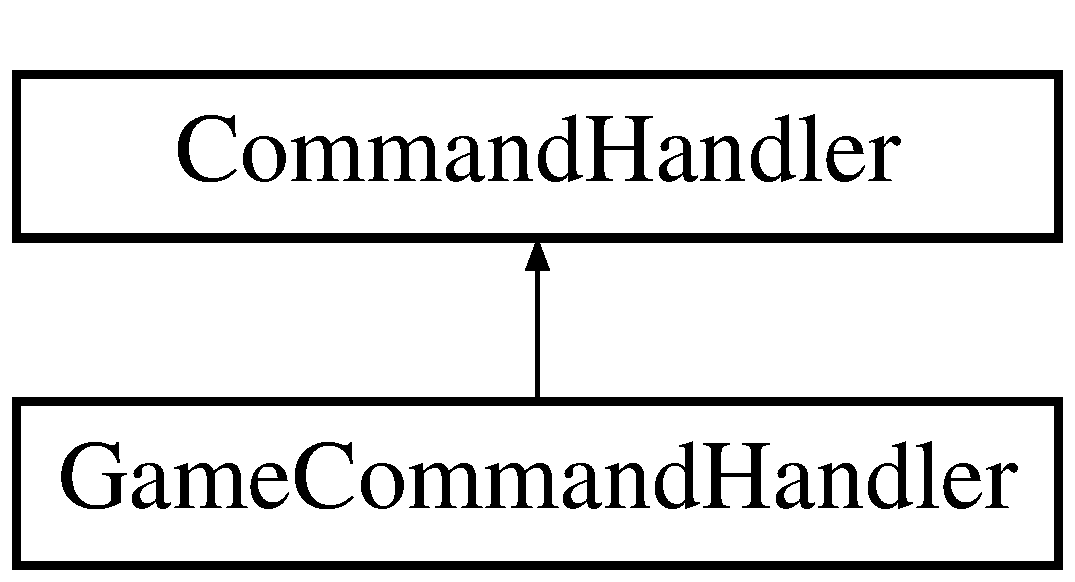
\includegraphics[height=2.000000cm]{class_game_command_handler}
\end{center}
\end{figure}
\subsection*{Public Member Functions}
\begin{DoxyCompactItemize}
\item 
\hypertarget{class_game_command_handler_a64214d5446cb173055d552a83c9c54bb}{{\bfseries Game\-Command\-Handler} (\hyperlink{class_game}{Game} \&game)}\label{class_game_command_handler_a64214d5446cb173055d552a83c9c54bb}

\end{DoxyCompactItemize}
\subsection*{Protected Member Functions}
\begin{DoxyCompactItemize}
\item 
\hypertarget{class_game_command_handler_a7afb31c523176bc0f1c7b2819d520a11}{virtual void {\bfseries player\-\_\-update\-\_\-to\-\_\-client} (const \hyperlink{class_player_update_to_client}{Player\-Update\-To\-Client} \&pe)}\label{class_game_command_handler_a7afb31c523176bc0f1c7b2819d520a11}

\item 
\hypertarget{class_game_command_handler_a4abebde7b787da05ca9611ee97377b06}{virtual void {\bfseries player\-\_\-accepted} (const \hyperlink{class_player_accepted}{Player\-Accepted} \&pe)}\label{class_game_command_handler_a4abebde7b787da05ca9611ee97377b06}

\item 
\hypertarget{class_game_command_handler_a0810bc6966823ed6fde896a8ac2a3bd1}{virtual void {\bfseries player\-\_\-rejected} (const \hyperlink{class_player_rejected}{Player\-Rejected} \&pe)}\label{class_game_command_handler_a0810bc6966823ed6fde896a8ac2a3bd1}

\item 
\hypertarget{class_game_command_handler_a6a87f9769f6b53aabea9800430951e4f}{virtual void {\bfseries player\-\_\-send\-\_\-message} (const \hyperlink{class_player_send_message}{Player\-Send\-Message} \&pe)}\label{class_game_command_handler_a6a87f9769f6b53aabea9800430951e4f}

\item 
\hypertarget{class_game_command_handler_a30a64a6bb2d2fb1d0df89b02777beb99}{virtual void {\bfseries player\-\_\-connected} (const \hyperlink{class_player_connected}{Player\-Connected} \&pe)}\label{class_game_command_handler_a30a64a6bb2d2fb1d0df89b02777beb99}

\item 
\hypertarget{class_game_command_handler_aab0f1e1376b0dd10c343597678cee387}{virtual void {\bfseries player\-\_\-disconnected} (const \hyperlink{class_player_disconnected}{Player\-Disconnected} \&pe)}\label{class_game_command_handler_aab0f1e1376b0dd10c343597678cee387}

\item 
\hypertarget{class_game_command_handler_a6dd8aba8b008733ea05b7854076c063b}{virtual void {\bfseries server\-\_\-entry\-\_\-list} (const \hyperlink{class_server_entry_list}{Server\-Entry\-List} \&pe)}\label{class_game_command_handler_a6dd8aba8b008733ea05b7854076c063b}

\item 
\hypertarget{class_game_command_handler_aebbb840794d2ea7b975ff313e0ecbec0}{virtual void {\bfseries load\-\_\-level} (const \hyperlink{class_load_level}{Load\-Level} \&pe)}\label{class_game_command_handler_aebbb840794d2ea7b975ff313e0ecbec0}

\item 
\hypertarget{class_game_command_handler_a9bf349f0b73c3af95b5ab708279d9e3b}{virtual void {\bfseries create\-\_\-target} (const \hyperlink{class_create_target}{Create\-Target} \&pe)}\label{class_game_command_handler_a9bf349f0b73c3af95b5ab708279d9e3b}

\item 
\hypertarget{class_game_command_handler_a7a0199bbf10f1167f42670cb648759ee}{virtual void {\bfseries score\-\_\-change} (const \hyperlink{class_score_change}{Score\-Change} \&pe)}\label{class_game_command_handler_a7a0199bbf10f1167f42670cb648759ee}

\item 
\hypertarget{class_game_command_handler_a420309474238a2692e518b01b9b65fb6}{virtual void {\bfseries destroy\-\_\-target} (const \hyperlink{class_destroy_target}{Destroy\-Target} \&pe)}\label{class_game_command_handler_a420309474238a2692e518b01b9b65fb6}

\end{DoxyCompactItemize}


The documentation for this class was generated from the following files\-:\begin{DoxyCompactItemize}
\item 
include/Game\-Command\-Handler.\-hpp\item 
src/Game\-Command\-Handler.\-cpp\end{DoxyCompactItemize}

\hypertarget{class_game_object}{\section{Game\-Object Class Reference}
\label{class_game_object}\index{Game\-Object@{Game\-Object}}
}
Inheritance diagram for Game\-Object\-:\begin{figure}[H]
\begin{center}
\leavevmode
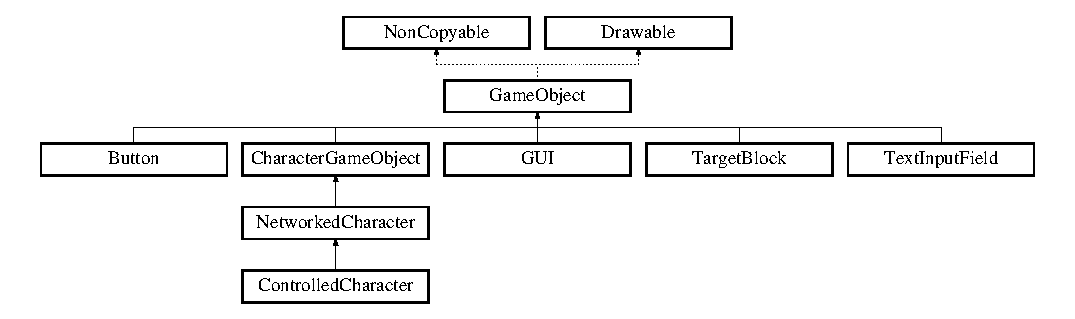
\includegraphics[height=3.835616cm]{class_game_object}
\end{center}
\end{figure}
\subsection*{Public Member Functions}
\begin{DoxyCompactItemize}
\item 
\hypertarget{class_game_object_a1e50d4cace9d1d2c12bfd4f73f43d089}{{\bfseries Game\-Object} (const std\-::string \&name)}\label{class_game_object_a1e50d4cace9d1d2c12bfd4f73f43d089}

\end{DoxyCompactItemize}
\subsection*{Static Public Member Functions}
\begin{DoxyCompactItemize}
\item 
\hypertarget{class_game_object_a95df6d5712b6de96dae66a26d72bb0df}{static void {\bfseries destroy} (\hyperlink{class_game_object}{Game\-Object} \&go)}\label{class_game_object_a95df6d5712b6de96dae66a26d72bb0df}

\end{DoxyCompactItemize}
\subsection*{Public Attributes}
\begin{DoxyCompactItemize}
\item 
\hypertarget{class_game_object_af542b33c8de269343e22c5629e6b66c0}{std\-::string {\bfseries name}}\label{class_game_object_af542b33c8de269343e22c5629e6b66c0}

\item 
\hypertarget{class_game_object_a104598c64b16c88712b0bec6e669ecf0}{\hyperlink{class_transform}{Transform} \& {\bfseries transform}}\label{class_game_object_a104598c64b16c88712b0bec6e669ecf0}

\end{DoxyCompactItemize}
\subsection*{Protected Member Functions}
\begin{DoxyCompactItemize}
\item 
\hypertarget{class_game_object_a4abb95a00e491aa09dc540f4bc9b9340}{virtual void {\bfseries start} ()}\label{class_game_object_a4abb95a00e491aa09dc540f4bc9b9340}

\item 
\hypertarget{class_game_object_ad4a07f19f6c5e2e71c89c07486f26244}{virtual void {\bfseries update} ()}\label{class_game_object_ad4a07f19f6c5e2e71c89c07486f26244}

\item 
\hypertarget{class_game_object_a3288cf2d607a7d44c3d9f0ac700cbda0}{virtual void {\bfseries draw} (sf\-::\-Render\-Target \&target, sf\-::\-Render\-States states) const }\label{class_game_object_a3288cf2d607a7d44c3d9f0ac700cbda0}

\item 
\hypertarget{class_game_object_a48bd07f9773dce443eb755477dee7dad}{virtual void {\bfseries on\-Destroy} ()}\label{class_game_object_a48bd07f9773dce443eb755477dee7dad}

\end{DoxyCompactItemize}
\subsection*{Protected Attributes}
\begin{DoxyCompactItemize}
\item 
\hypertarget{class_game_object_afac7336fdac6c19da71c790c61b509df}{bool {\bfseries is\-Marked\-For\-Destroy}}\label{class_game_object_afac7336fdac6c19da71c790c61b509df}

\end{DoxyCompactItemize}
\subsection*{Friends}
\begin{DoxyCompactItemize}
\item 
\hypertarget{class_game_object_a032858ae1fe02d2d1170981c2af2d67c}{class {\bfseries Scene}}\label{class_game_object_a032858ae1fe02d2d1170981c2af2d67c}

\item 
\hypertarget{class_game_object_af851b4d9aacd1a871da33592334b8d72}{class {\bfseries Transform}}\label{class_game_object_af851b4d9aacd1a871da33592334b8d72}

\end{DoxyCompactItemize}


The documentation for this class was generated from the following files\-:\begin{DoxyCompactItemize}
\item 
include/Game\-Object.\-hpp\item 
src/Game\-Object.\-cpp\end{DoxyCompactItemize}

\hypertarget{class_g_u_i}{\section{G\-U\-I Class Reference}
\label{class_g_u_i}\index{G\-U\-I@{G\-U\-I}}
}
Inheritance diagram for G\-U\-I\-:\begin{figure}[H]
\begin{center}
\leavevmode
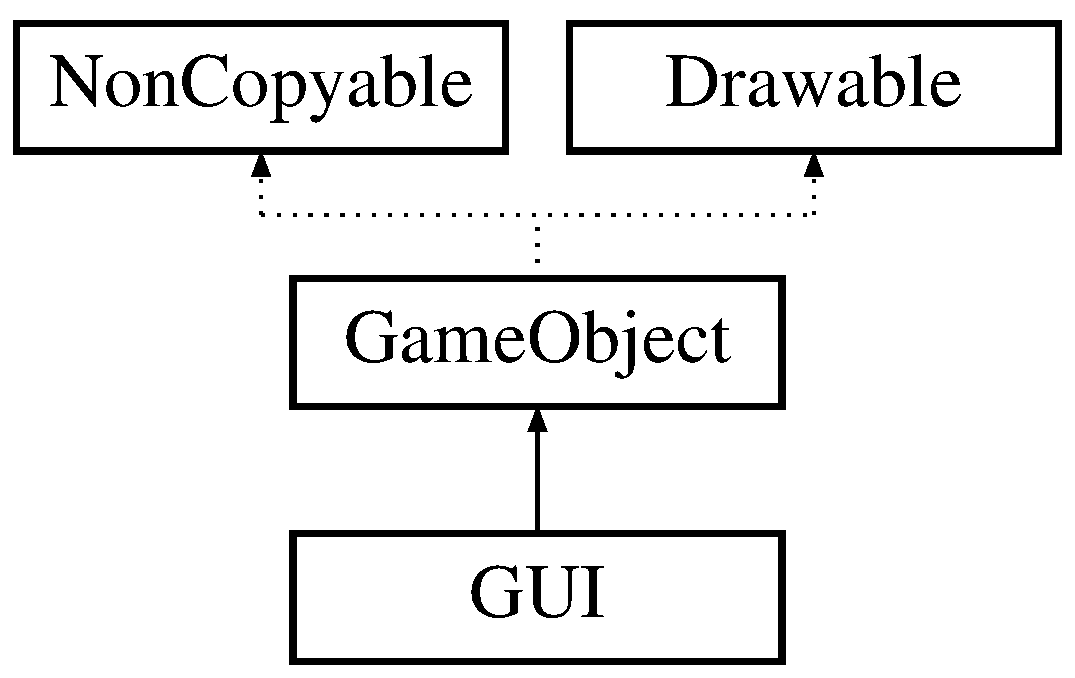
\includegraphics[height=3.000000cm]{class_g_u_i}
\end{center}
\end{figure}
\subsection*{Public Member Functions}
\begin{DoxyCompactItemize}
\item 
\hypertarget{class_g_u_i_afbedd68995919c50a7298de4735b77c6}{void {\bfseries set\-Game} (\hyperlink{class_game}{Game} $\ast$game)}\label{class_g_u_i_afbedd68995919c50a7298de4735b77c6}

\item 
\hypertarget{class_g_u_i_aa04da479a7d4af5cbf0e4a7d821026d8}{const sf\-::\-Font \& {\bfseries get\-Font} () const }\label{class_g_u_i_aa04da479a7d4af5cbf0e4a7d821026d8}

\end{DoxyCompactItemize}
\subsection*{Public Attributes}
\begin{DoxyCompactItemize}
\item 
\hypertarget{class_g_u_i_ac7d6f381a87bc0ac9644f3abd14bc5f0}{sf\-::\-Text {\bfseries info\-Field}}\label{class_g_u_i_ac7d6f381a87bc0ac9644f3abd14bc5f0}

\end{DoxyCompactItemize}
\subsection*{Static Public Attributes}
\begin{DoxyCompactItemize}
\item 
\hypertarget{class_g_u_i_a0df934366b2f996721ba92fd751ec873}{static \hyperlink{class_g_u_i}{G\-U\-I} $\ast$ {\bfseries instance}}\label{class_g_u_i_a0df934366b2f996721ba92fd751ec873}

\end{DoxyCompactItemize}
\subsection*{Protected Member Functions}
\begin{DoxyCompactItemize}
\item 
\hypertarget{class_g_u_i_a947e568bf884a8798e3e368417f662c7}{virtual void {\bfseries update} ()}\label{class_g_u_i_a947e568bf884a8798e3e368417f662c7}

\item 
\hypertarget{class_g_u_i_a8715710585e90991ac80329217538f27}{virtual void {\bfseries draw} (sf\-::\-Render\-Target \&target, sf\-::\-Render\-States states) const }\label{class_g_u_i_a8715710585e90991ac80329217538f27}

\end{DoxyCompactItemize}
\subsection*{Additional Inherited Members}


The documentation for this class was generated from the following files\-:\begin{DoxyCompactItemize}
\item 
include/G\-U\-I.\-hpp\item 
src/G\-U\-I.\-cpp\end{DoxyCompactItemize}

\hypertarget{struct_hash}{\section{Hash Struct Reference}
\label{struct_hash}\index{Hash@{Hash}}
}
\subsection*{Classes}
\begin{DoxyCompactItemize}
\item 
struct \hyperlink{struct_hash_1_1__ht}{\-\_\-ht}
\end{DoxyCompactItemize}
\subsection*{Public Attributes}
\begin{DoxyCompactItemize}
\item 
\hypertarget{struct_hash_a072258e24a38e09175f1308deb013bc8}{unsigned int {\bfseries htsize}}\label{struct_hash_a072258e24a38e09175f1308deb013bc8}

\item 
\hypertarget{struct_hash_a7ab16f173cdc347ffbe39eaa85ee6fda}{unsigned int {\bfseries count}}\label{struct_hash_a7ab16f173cdc347ffbe39eaa85ee6fda}

\item 
\hypertarget{struct_hash_a2cfc9936ca2a624c6492ab6557f4705b}{\hyperlink{struct_hash_elem}{Hash\-Elem} $\ast$ {\bfseries first}}\label{struct_hash_a2cfc9936ca2a624c6492ab6557f4705b}

\item 
\hypertarget{struct_hash_ac0f36e03746a3fe69643db08d93bc0c4}{struct \hyperlink{struct_hash_1_1__ht}{Hash\-::\-\_\-ht} $\ast$ {\bfseries ht}}\label{struct_hash_ac0f36e03746a3fe69643db08d93bc0c4}

\end{DoxyCompactItemize}


The documentation for this struct was generated from the following file\-:\begin{DoxyCompactItemize}
\item 
src/sqlite3.\-c\end{DoxyCompactItemize}

\hypertarget{struct_hash_elem}{\section{Hash\-Elem Struct Reference}
\label{struct_hash_elem}\index{Hash\-Elem@{Hash\-Elem}}
}
\subsection*{Public Attributes}
\begin{DoxyCompactItemize}
\item 
\hypertarget{struct_hash_elem_a2d28fad45ff21ffb8a02a7133df860fd}{\hyperlink{struct_hash_elem}{Hash\-Elem} $\ast$ {\bfseries next}}\label{struct_hash_elem_a2d28fad45ff21ffb8a02a7133df860fd}

\item 
\hypertarget{struct_hash_elem_ae4d011c0dc807a3c100ccdb927dd0ba9}{\hyperlink{struct_hash_elem}{Hash\-Elem} $\ast$ {\bfseries prev}}\label{struct_hash_elem_ae4d011c0dc807a3c100ccdb927dd0ba9}

\item 
\hypertarget{struct_hash_elem_ac7e80f63ba2f82457ff68aa0cd360365}{void $\ast$ {\bfseries data}}\label{struct_hash_elem_ac7e80f63ba2f82457ff68aa0cd360365}

\item 
\hypertarget{struct_hash_elem_a9c33a7c8ac467a5547a123338daf61f4}{const char $\ast$ {\bfseries p\-Key}}\label{struct_hash_elem_a9c33a7c8ac467a5547a123338daf61f4}

\item 
\hypertarget{struct_hash_elem_a12c1252e6aa2958f73e2ef969c9a3d81}{int {\bfseries n\-Key}}\label{struct_hash_elem_a12c1252e6aa2958f73e2ef969c9a3d81}

\end{DoxyCompactItemize}


The documentation for this struct was generated from the following file\-:\begin{DoxyCompactItemize}
\item 
src/sqlite3.\-c\end{DoxyCompactItemize}

\hypertarget{struct_id_list}{\section{Id\-List Struct Reference}
\label{struct_id_list}\index{Id\-List@{Id\-List}}
}
\subsection*{Classes}
\begin{DoxyCompactItemize}
\item 
struct \hyperlink{struct_id_list_1_1_id_list__item}{Id\-List\-\_\-item}
\end{DoxyCompactItemize}
\subsection*{Public Attributes}
\begin{DoxyCompactItemize}
\item 
\hypertarget{struct_id_list_ad33082fd71286c1159711a1a3e979763}{struct \hyperlink{struct_id_list_1_1_id_list__item}{Id\-List\-::\-Id\-List\-\_\-item} $\ast$ {\bfseries a}}\label{struct_id_list_ad33082fd71286c1159711a1a3e979763}

\item 
\hypertarget{struct_id_list_afb785717796d8b3c72d1ae682dcb6ff0}{int {\bfseries n\-Id}}\label{struct_id_list_afb785717796d8b3c72d1ae682dcb6ff0}

\end{DoxyCompactItemize}


The documentation for this struct was generated from the following file\-:\begin{DoxyCompactItemize}
\item 
src/sqlite3.\-c\end{DoxyCompactItemize}

\hypertarget{struct_id_list_1_1_id_list__item}{\section{Id\-List\-:\-:Id\-List\-\_\-item Struct Reference}
\label{struct_id_list_1_1_id_list__item}\index{Id\-List\-::\-Id\-List\-\_\-item@{Id\-List\-::\-Id\-List\-\_\-item}}
}
\subsection*{Public Attributes}
\begin{DoxyCompactItemize}
\item 
\hypertarget{struct_id_list_1_1_id_list__item_acd44e1182dc46441939cd6a5d935724c}{char $\ast$ {\bfseries z\-Name}}\label{struct_id_list_1_1_id_list__item_acd44e1182dc46441939cd6a5d935724c}

\item 
\hypertarget{struct_id_list_1_1_id_list__item_a869d1a5ee03bcb018e38fae6c9ac0572}{int {\bfseries idx}}\label{struct_id_list_1_1_id_list__item_a869d1a5ee03bcb018e38fae6c9ac0572}

\end{DoxyCompactItemize}


The documentation for this struct was generated from the following file\-:\begin{DoxyCompactItemize}
\item 
src/sqlite3.\-c\end{DoxyCompactItemize}

\hypertarget{struct_incrblob}{\section{Incrblob Struct Reference}
\label{struct_incrblob}\index{Incrblob@{Incrblob}}
}
\subsection*{Public Attributes}
\begin{DoxyCompactItemize}
\item 
\hypertarget{struct_incrblob_a46fa093e5241305f28d02926f8d0846f}{int {\bfseries flags}}\label{struct_incrblob_a46fa093e5241305f28d02926f8d0846f}

\item 
\hypertarget{struct_incrblob_ab1e1439df086208173fa97003f0ee02b}{int {\bfseries n\-Byte}}\label{struct_incrblob_ab1e1439df086208173fa97003f0ee02b}

\item 
\hypertarget{struct_incrblob_af8e71744f43178967460b9f402e7fafd}{int {\bfseries i\-Offset}}\label{struct_incrblob_af8e71744f43178967460b9f402e7fafd}

\item 
\hypertarget{struct_incrblob_a398a322b061fb9952bc155026976ba51}{int {\bfseries i\-Col}}\label{struct_incrblob_a398a322b061fb9952bc155026976ba51}

\item 
\hypertarget{struct_incrblob_af5a24b18473d1449c8c3fe7d826de59a}{\hyperlink{struct_bt_cursor}{Bt\-Cursor} $\ast$ {\bfseries p\-Csr}}\label{struct_incrblob_af5a24b18473d1449c8c3fe7d826de59a}

\item 
\hypertarget{struct_incrblob_a8b7b39c9372db552add74c69f14a61a3}{sqlite3\-\_\-stmt $\ast$ {\bfseries p\-Stmt}}\label{struct_incrblob_a8b7b39c9372db552add74c69f14a61a3}

\item 
\hypertarget{struct_incrblob_a9d3fe0b0229b75b9d0f9ee8e6545b5bc}{\hyperlink{structsqlite3}{sqlite3} $\ast$ {\bfseries db}}\label{struct_incrblob_a9d3fe0b0229b75b9d0f9ee8e6545b5bc}

\end{DoxyCompactItemize}


The documentation for this struct was generated from the following file\-:\begin{DoxyCompactItemize}
\item 
src/sqlite3.\-c\end{DoxyCompactItemize}

\hypertarget{struct_index}{\section{Index Struct Reference}
\label{struct_index}\index{Index@{Index}}
}
\subsection*{Public Attributes}
\begin{DoxyCompactItemize}
\item 
\hypertarget{struct_index_a8848cddf6e09f22e3b794ec019082ced}{char $\ast$ {\bfseries z\-Name}}\label{struct_index_a8848cddf6e09f22e3b794ec019082ced}

\item 
\hypertarget{struct_index_acbb125339b02ca6819dd2e382de2d639}{int $\ast$ {\bfseries ai\-Column}}\label{struct_index_acbb125339b02ca6819dd2e382de2d639}

\item 
\hypertarget{struct_index_aa408555f4da96ca1fae741ff6d33a3bf}{t\-Rowcnt $\ast$ {\bfseries ai\-Row\-Est}}\label{struct_index_aa408555f4da96ca1fae741ff6d33a3bf}

\item 
\hypertarget{struct_index_a01c6d4da27cba325ca58f333f87a6f44}{\hyperlink{struct_table}{Table} $\ast$ {\bfseries p\-Table}}\label{struct_index_a01c6d4da27cba325ca58f333f87a6f44}

\item 
\hypertarget{struct_index_af076df9f74dd836001c0a59d27274c0e}{char $\ast$ {\bfseries z\-Col\-Aff}}\label{struct_index_af076df9f74dd836001c0a59d27274c0e}

\item 
\hypertarget{struct_index_a115a17d236bd277d59dd5ea030954c3e}{\hyperlink{struct_index}{Index} $\ast$ {\bfseries p\-Next}}\label{struct_index_a115a17d236bd277d59dd5ea030954c3e}

\item 
\hypertarget{struct_index_af14f5ddd57eab2aba63dcb5db2aa92af}{\hyperlink{struct_schema}{Schema} $\ast$ {\bfseries p\-Schema}}\label{struct_index_af14f5ddd57eab2aba63dcb5db2aa92af}

\item 
\hypertarget{struct_index_a0a3fc87b53193995f59c9657443e9a99}{u8 $\ast$ {\bfseries a\-Sort\-Order}}\label{struct_index_a0a3fc87b53193995f59c9657443e9a99}

\item 
\hypertarget{struct_index_ab690ebb96c0329896b0fe2ab56813b88}{char $\ast$$\ast$ {\bfseries az\-Coll}}\label{struct_index_ab690ebb96c0329896b0fe2ab56813b88}

\item 
\hypertarget{struct_index_ac583449830c285a52d1fd10b8c890162}{int {\bfseries n\-Column}}\label{struct_index_ac583449830c285a52d1fd10b8c890162}

\item 
\hypertarget{struct_index_af895a09c01701021c3e36362c04a1ae6}{int {\bfseries tnum}}\label{struct_index_af895a09c01701021c3e36362c04a1ae6}

\item 
\hypertarget{struct_index_ae8bf87d0414e5c46b86192cfbdd271a7}{u8 {\bfseries on\-Error}}\label{struct_index_ae8bf87d0414e5c46b86192cfbdd271a7}

\item 
\hypertarget{struct_index_a1fa09182749b6e07b2555d5b3dffb91d}{u8 {\bfseries auto\-Index}}\label{struct_index_a1fa09182749b6e07b2555d5b3dffb91d}

\item 
\hypertarget{struct_index_a1a3114080bcca1d9dd23ce5755d4e4e8}{u8 {\bfseries b\-Unordered}}\label{struct_index_a1a3114080bcca1d9dd23ce5755d4e4e8}

\end{DoxyCompactItemize}


The documentation for this struct was generated from the following file\-:\begin{DoxyCompactItemize}
\item 
src/sqlite3.\-c\end{DoxyCompactItemize}

\hypertarget{struct_index_sample}{\section{Index\-Sample Struct Reference}
\label{struct_index_sample}\index{Index\-Sample@{Index\-Sample}}
}
\subsection*{Public Attributes}
\begin{DoxyCompactItemize}
\item 
\hypertarget{struct_index_sample_a2339218a9b5b05d45ef683ead174b2bd}{\begin{tabbing}
xx\=xx\=xx\=xx\=xx\=xx\=xx\=xx\=xx\=\kill
union \{\\
\>char $\ast$ {\bfseries z}\\
\>double {\bfseries r}\\
\>i64 {\bfseries i}\\
\} {\bfseries u}}\label{struct_index_sample_a2339218a9b5b05d45ef683ead174b2bd}
\\

\end{tabbing}\item 
\hypertarget{struct_index_sample_a369f346d71bab2423e015d0fb6809290}{u8 {\bfseries e\-Type}}\label{struct_index_sample_a369f346d71bab2423e015d0fb6809290}

\item 
\hypertarget{struct_index_sample_a216647c71443cdd198787afc6e1a3951}{int {\bfseries n\-Byte}}\label{struct_index_sample_a216647c71443cdd198787afc6e1a3951}

\item 
\hypertarget{struct_index_sample_aca6a7f1338b7a316ec29e8968568c3d1}{t\-Rowcnt {\bfseries n\-Eq}}\label{struct_index_sample_aca6a7f1338b7a316ec29e8968568c3d1}

\item 
\hypertarget{struct_index_sample_a5e2391cced4ee840bc7e168372a836c5}{t\-Rowcnt {\bfseries n\-Lt}}\label{struct_index_sample_a5e2391cced4ee840bc7e168372a836c5}

\item 
\hypertarget{struct_index_sample_ab24fbf5f95e260735c63c8b7986126ca}{t\-Rowcnt {\bfseries n\-D\-Lt}}\label{struct_index_sample_ab24fbf5f95e260735c63c8b7986126ca}

\end{DoxyCompactItemize}


The documentation for this struct was generated from the following file\-:\begin{DoxyCompactItemize}
\item 
src/sqlite3.\-c\end{DoxyCompactItemize}

\hypertarget{struct_init_data}{\section{Init\-Data Struct Reference}
\label{struct_init_data}\index{Init\-Data@{Init\-Data}}
}
\subsection*{Public Attributes}
\begin{DoxyCompactItemize}
\item 
\hypertarget{struct_init_data_adc9e29c56e0392076e92d7f4b29fa272}{\hyperlink{structsqlite3}{sqlite3} $\ast$ {\bfseries db}}\label{struct_init_data_adc9e29c56e0392076e92d7f4b29fa272}

\item 
\hypertarget{struct_init_data_aa8aef34241ec214f038b38932ffe1357}{char $\ast$$\ast$ {\bfseries pz\-Err\-Msg}}\label{struct_init_data_aa8aef34241ec214f038b38932ffe1357}

\item 
\hypertarget{struct_init_data_ad6c7953b49d351cd9fb14e3394010689}{int {\bfseries i\-Db}}\label{struct_init_data_ad6c7953b49d351cd9fb14e3394010689}

\item 
\hypertarget{struct_init_data_a627153a3de2c4d159ae44ebc03961592}{int {\bfseries rc}}\label{struct_init_data_a627153a3de2c4d159ae44ebc03961592}

\end{DoxyCompactItemize}


The documentation for this struct was generated from the following file\-:\begin{DoxyCompactItemize}
\item 
src/sqlite3.\-c\end{DoxyCompactItemize}

\hypertarget{struct_integrity_ck}{\section{Integrity\-Ck Struct Reference}
\label{struct_integrity_ck}\index{Integrity\-Ck@{Integrity\-Ck}}
}
\subsection*{Public Attributes}
\begin{DoxyCompactItemize}
\item 
\hypertarget{struct_integrity_ck_a65f03f54514f504bd871bb2ccd3da188}{\hyperlink{struct_bt_shared}{Bt\-Shared} $\ast$ {\bfseries p\-Bt}}\label{struct_integrity_ck_a65f03f54514f504bd871bb2ccd3da188}

\item 
\hypertarget{struct_integrity_ck_a87e7f8b012b61b61fae359269cbacce4}{\hyperlink{struct_pager}{Pager} $\ast$ {\bfseries p\-Pager}}\label{struct_integrity_ck_a87e7f8b012b61b61fae359269cbacce4}

\item 
\hypertarget{struct_integrity_ck_a317f80aef5842ad69df75b55e14118d1}{u8 $\ast$ {\bfseries a\-Pg\-Ref}}\label{struct_integrity_ck_a317f80aef5842ad69df75b55e14118d1}

\item 
\hypertarget{struct_integrity_ck_a04f496ef7239aea6dccb6a861bb5a798}{Pgno {\bfseries n\-Page}}\label{struct_integrity_ck_a04f496ef7239aea6dccb6a861bb5a798}

\item 
\hypertarget{struct_integrity_ck_a9daa97cdcb1366c503451ab2af9e7ba6}{int {\bfseries mx\-Err}}\label{struct_integrity_ck_a9daa97cdcb1366c503451ab2af9e7ba6}

\item 
\hypertarget{struct_integrity_ck_a52c815a1d19be87d0ab4dc0a4e4d38e2}{int {\bfseries n\-Err}}\label{struct_integrity_ck_a52c815a1d19be87d0ab4dc0a4e4d38e2}

\item 
\hypertarget{struct_integrity_ck_a8e448c1d6483a0326a7ec39291782030}{int {\bfseries malloc\-Failed}}\label{struct_integrity_ck_a8e448c1d6483a0326a7ec39291782030}

\item 
\hypertarget{struct_integrity_ck_a1e9b79bb1d7b22a840001333200a950e}{\hyperlink{struct_str_accum}{Str\-Accum} {\bfseries err\-Msg}}\label{struct_integrity_ck_a1e9b79bb1d7b22a840001333200a950e}

\end{DoxyCompactItemize}


The documentation for this struct was generated from the following file\-:\begin{DoxyCompactItemize}
\item 
src/sqlite3.\-c\end{DoxyCompactItemize}

\hypertarget{struct_key_info}{\section{Key\-Info Struct Reference}
\label{struct_key_info}\index{Key\-Info@{Key\-Info}}
}
\subsection*{Public Attributes}
\begin{DoxyCompactItemize}
\item 
\hypertarget{struct_key_info_af2e7a3a411f5ca1ccf6de77d320b59db}{\hyperlink{structsqlite3}{sqlite3} $\ast$ {\bfseries db}}\label{struct_key_info_af2e7a3a411f5ca1ccf6de77d320b59db}

\item 
\hypertarget{struct_key_info_a37972825f9a148668e979be12465e832}{u8 {\bfseries enc}}\label{struct_key_info_a37972825f9a148668e979be12465e832}

\item 
\hypertarget{struct_key_info_af70436487a95e445d540bfc4ca1d3f0b}{u16 {\bfseries n\-Field}}\label{struct_key_info_af70436487a95e445d540bfc4ca1d3f0b}

\item 
\hypertarget{struct_key_info_ac5fe4bd0172a1f11f41f678528a7b21e}{u8 $\ast$ {\bfseries a\-Sort\-Order}}\label{struct_key_info_ac5fe4bd0172a1f11f41f678528a7b21e}

\item 
\hypertarget{struct_key_info_ad43aa024fca5a065e75d8e24b231adcb}{\hyperlink{struct_coll_seq}{Coll\-Seq} $\ast$ {\bfseries a\-Coll} \mbox{[}1\mbox{]}}\label{struct_key_info_ad43aa024fca5a065e75d8e24b231adcb}

\end{DoxyCompactItemize}


The documentation for this struct was generated from the following file\-:\begin{DoxyCompactItemize}
\item 
src/sqlite3.\-c\end{DoxyCompactItemize}

\hypertarget{class_key_state}{\section{Key\-State Class Reference}
\label{class_key_state}\index{Key\-State@{Key\-State}}
}
\subsection*{Public Member Functions}
\begin{DoxyCompactItemize}
\item 
\hypertarget{class_key_state_a225049e5d6f1bc6e914c81d7dc6f97b2}{{\bfseries Key\-State} (bool up, bool down, bool left, bool right)}\label{class_key_state_a225049e5d6f1bc6e914c81d7dc6f97b2}

\item 
\hypertarget{class_key_state_ac1327d75edde0c7b5daf5e4009c4fc6f}{bool {\bfseries operator==} (const \hyperlink{class_key_state}{Key\-State} \&other)}\label{class_key_state_ac1327d75edde0c7b5daf5e4009c4fc6f}

\item 
\hypertarget{class_key_state_a93b8cf2e65c8055803f1633cb1c74776}{bool {\bfseries operator!=} (const \hyperlink{class_key_state}{Key\-State} \&other)}\label{class_key_state_a93b8cf2e65c8055803f1633cb1c74776}

\end{DoxyCompactItemize}
\subsection*{Public Attributes}
\begin{DoxyCompactItemize}
\item 
\hypertarget{class_key_state_aee741b57639d1b11b63c2e40416e482c}{bool {\bfseries up}}\label{class_key_state_aee741b57639d1b11b63c2e40416e482c}

\item 
\hypertarget{class_key_state_a85ea4df350911a6ebe8314418b190071}{bool {\bfseries down}}\label{class_key_state_a85ea4df350911a6ebe8314418b190071}

\item 
\hypertarget{class_key_state_a44036306a5c13b07ae998e4aea86f52d}{bool {\bfseries left}}\label{class_key_state_a44036306a5c13b07ae998e4aea86f52d}

\item 
\hypertarget{class_key_state_a15f5326fae7f6f1b65389a4f8bac13ef}{bool {\bfseries right}}\label{class_key_state_a15f5326fae7f6f1b65389a4f8bac13ef}

\end{DoxyCompactItemize}
\subsection*{Friends}
\begin{DoxyCompactItemize}
\item 
\hypertarget{class_key_state_ab41f00181962266823d9a1ea779294d6}{sf\-::\-Packet \& {\bfseries operator$<$$<$} (sf\-::\-Packet \&pack, const \hyperlink{class_key_state}{Key\-State} \&key\-State)}\label{class_key_state_ab41f00181962266823d9a1ea779294d6}

\item 
\hypertarget{class_key_state_aa508ce1c8f48dab284fd0b64074b78f4}{sf\-::\-Packet \& {\bfseries operator$>$$>$} (sf\-::\-Packet \&pack, \hyperlink{class_key_state}{Key\-State} \&key\-State)}\label{class_key_state_aa508ce1c8f48dab284fd0b64074b78f4}

\item 
\hypertarget{class_key_state_a5ec231cfca1b4c327e92ad9d18a3f205}{std\-::ostream \& {\bfseries operator$<$$<$} (std\-::ostream \&out, const \hyperlink{class_key_state}{Key\-State} \&key\-State)}\label{class_key_state_a5ec231cfca1b4c327e92ad9d18a3f205}

\end{DoxyCompactItemize}


The documentation for this class was generated from the following files\-:\begin{DoxyCompactItemize}
\item 
include/Key\-State.\-hpp\item 
src/Key\-State.\-cpp\end{DoxyCompactItemize}

\hypertarget{class_level}{\section{Level Class Reference}
\label{class_level}\index{Level@{Level}}
}
\subsection*{Public Types}
\begin{DoxyCompactItemize}
\item 
\hypertarget{class_level_abdb7997d6b026545c865baa7281b79c7}{typedef std\-::vector$<$ int $>$ {\bfseries Ints}}\label{class_level_abdb7997d6b026545c865baa7281b79c7}

\end{DoxyCompactItemize}
\subsection*{Public Member Functions}
\begin{DoxyCompactItemize}
\item 
\hypertarget{class_level_a209d4cda525298e007ac0e0bf54ae040}{const std\-::vector$<$ int $>$ \& {\bfseries get\-Level\-Array} () const }\label{class_level_a209d4cda525298e007ac0e0bf54ae040}

\item 
\hypertarget{class_level_a820319e6158473834e215bb709976d32}{bool {\bfseries get\-Loaded} () const }\label{class_level_a820319e6158473834e215bb709976d32}

\item 
\hypertarget{class_level_a28bd20dfbde4b23425325645cfe0c085}{int {\bfseries to\-Index} (glm\-::vec2 position) const }\label{class_level_a28bd20dfbde4b23425325645cfe0c085}

\item 
\hypertarget{class_level_a237518a6fdffb58f2696a12b038a129e}{int {\bfseries get\-Value} (int index) const }\label{class_level_a237518a6fdffb58f2696a12b038a129e}

\item 
\hypertarget{class_level_aa0da8924927f803ab5beef12df6d586f}{bool {\bfseries is\-Walkable} (int value) const }\label{class_level_aa0da8924927f803ab5beef12df6d586f}

\item 
\hypertarget{class_level_ad71b68776ad764243aa34ceb61edbf4b}{void \hyperlink{class_level_ad71b68776ad764243aa34ceb61edbf4b}{load\-Level\-Named} (const std\-::string \&name)}\label{class_level_ad71b68776ad764243aa34ceb61edbf4b}

\begin{DoxyCompactList}\small\item\em -\/-\/-\/-\/-\/-\/-\/-\/-\/-\/-\/-\/-\/-\/-\/-\/-\/-\/-\/-\/-\/-\/-\/-\/-\/-\/-\/-\/-\/-\/-\/-\/-\/-\/-\/-\/-\/-\/-\/-\/-\/-\/-\/-\/-\/-\/-\/-\/-\/---T\-E\-M\-P\-O\-R\-A\-R\-Y \end{DoxyCompactList}\item 
\hypertarget{class_level_aa1bea269cde46a448324e43dd2a480da}{glm\-::vec2 {\bfseries get\-Start\-Pos} () const }\label{class_level_aa1bea269cde46a448324e43dd2a480da}

\item 
\hypertarget{class_level_a35c152b4451c6e98276a923bcaff54be}{const std\-::vector$<$ glm\-::vec2 $>$ \& {\bfseries get\-Object\-Positions} () const }\label{class_level_a35c152b4451c6e98276a923bcaff54be}

\item 
\hypertarget{class_level_a6e8b4ec8dc8a2fe3d59eaddaa8ad0a29}{std\-::string {\bfseries get\-Loaded\-Level\-Name} () const }\label{class_level_a6e8b4ec8dc8a2fe3d59eaddaa8ad0a29}

\item 
\hypertarget{class_level_a78f28f8afdcc244f5e4bba1a93876de0}{std\-::string {\bfseries level\-To\-String} ()}\label{class_level_a78f28f8afdcc244f5e4bba1a93876de0}

\item 
\hypertarget{class_level_a956b87cc7a28078b565bb510e8316d8d}{const sf\-::\-Texture $\ast$ {\bfseries get\-Texture} ()}\label{class_level_a956b87cc7a28078b565bb510e8316d8d}

\end{DoxyCompactItemize}


The documentation for this class was generated from the following files\-:\begin{DoxyCompactItemize}
\item 
include/Level.\-hpp\item 
src/Level.\-cpp\end{DoxyCompactItemize}

\hypertarget{struct_like_op}{\section{Like\-Op Struct Reference}
\label{struct_like_op}\index{Like\-Op@{Like\-Op}}
}
\subsection*{Public Attributes}
\begin{DoxyCompactItemize}
\item 
\hypertarget{struct_like_op_a02dccb0eea9610285333434a755acae8}{\hyperlink{struct_token}{Token} {\bfseries e\-Operator}}\label{struct_like_op_a02dccb0eea9610285333434a755acae8}

\item 
\hypertarget{struct_like_op_a09daccf65c917f32e8b60b347e8893cf}{int {\bfseries b\-Not}}\label{struct_like_op_a09daccf65c917f32e8b60b347e8893cf}

\end{DoxyCompactItemize}


The documentation for this struct was generated from the following file\-:\begin{DoxyCompactItemize}
\item 
src/sqlite3.\-c\end{DoxyCompactItemize}

\hypertarget{struct_limit_val}{\section{Limit\-Val Struct Reference}
\label{struct_limit_val}\index{Limit\-Val@{Limit\-Val}}
}
\subsection*{Public Attributes}
\begin{DoxyCompactItemize}
\item 
\hypertarget{struct_limit_val_a96094d1b395a3f455263ff5907d72ed6}{\hyperlink{struct_expr}{Expr} $\ast$ {\bfseries p\-Limit}}\label{struct_limit_val_a96094d1b395a3f455263ff5907d72ed6}

\item 
\hypertarget{struct_limit_val_a43dedf453a8e5cb8091fcde524a7c736}{\hyperlink{struct_expr}{Expr} $\ast$ {\bfseries p\-Offset}}\label{struct_limit_val_a43dedf453a8e5cb8091fcde524a7c736}

\end{DoxyCompactItemize}


The documentation for this struct was generated from the following file\-:\begin{DoxyCompactItemize}
\item 
src/sqlite3.\-c\end{DoxyCompactItemize}

\hypertarget{class_load_level}{\section{Load\-Level Class Reference}
\label{class_load_level}\index{Load\-Level@{Load\-Level}}
}
Inheritance diagram for Load\-Level\-:\begin{figure}[H]
\begin{center}
\leavevmode
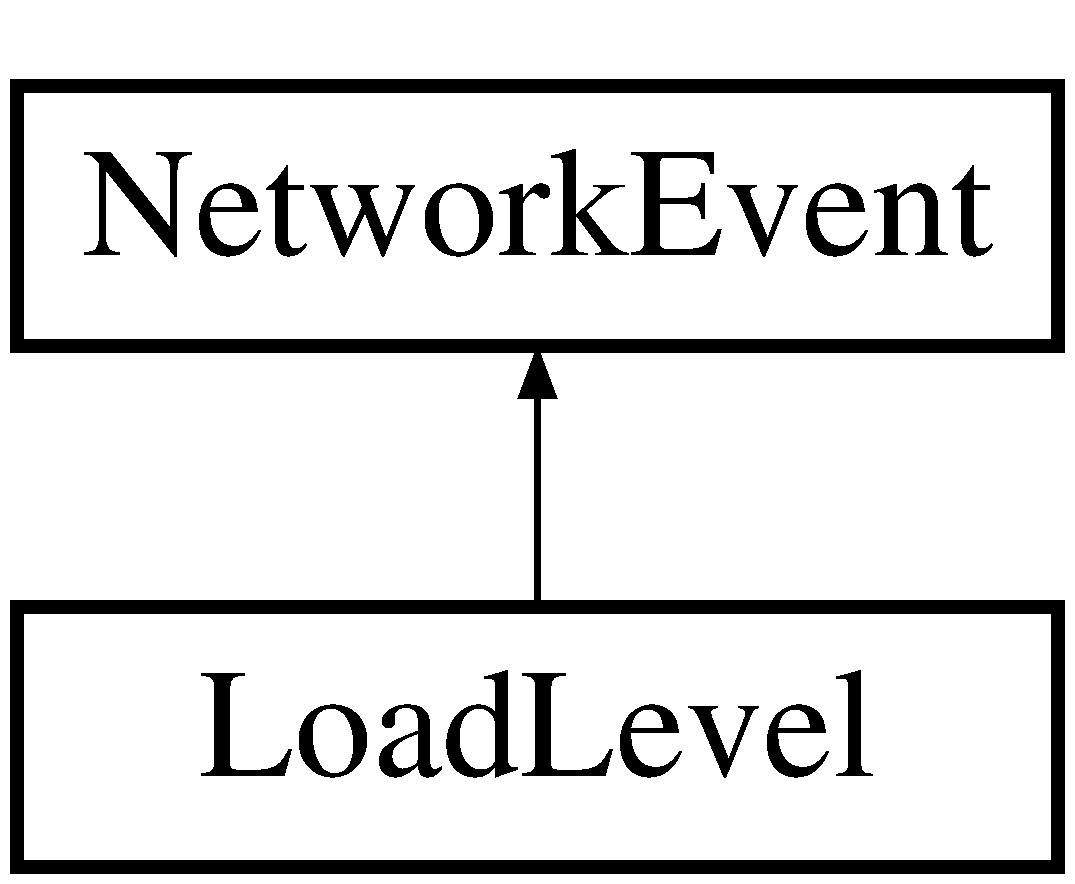
\includegraphics[height=2.000000cm]{class_load_level}
\end{center}
\end{figure}
\subsection*{Public Member Functions}
\begin{DoxyCompactItemize}
\item 
\hypertarget{class_load_level_a851258beaca8df111c68b57e0ecc466a}{virtual sf\-::\-Int32 {\bfseries get\-Command} () const }\label{class_load_level_a851258beaca8df111c68b57e0ecc466a}

\end{DoxyCompactItemize}
\subsection*{Public Attributes}
\begin{DoxyCompactItemize}
\item 
\hypertarget{class_load_level_a6d6fbda9be04ed3d4458db1b82b2c1cd}{std\-::string {\bfseries level\-Name}}\label{class_load_level_a6d6fbda9be04ed3d4458db1b82b2c1cd}

\end{DoxyCompactItemize}
\subsection*{Friends}
\begin{DoxyCompactItemize}
\item 
\hypertarget{class_load_level_a1de1314296b1d080ca8563ad2278c35a}{sf\-::\-Packet \& {\bfseries operator$<$$<$} (sf\-::\-Packet \&lhs, const \hyperlink{class_load_level}{Load\-Level} \&rhs)}\label{class_load_level_a1de1314296b1d080ca8563ad2278c35a}

\item 
\hypertarget{class_load_level_ac41ff97641eab59514df5bbf1ca459d9}{sf\-::\-Packet \& {\bfseries operator$>$$>$} (sf\-::\-Packet \&lhs, \hyperlink{class_load_level}{Load\-Level} \&rhs)}\label{class_load_level_ac41ff97641eab59514df5bbf1ca459d9}

\end{DoxyCompactItemize}
\subsection*{Additional Inherited Members}


The documentation for this class was generated from the following file\-:\begin{DoxyCompactItemize}
\item 
include/Network\-Events.\-h\end{DoxyCompactItemize}

\hypertarget{class_local_player_info}{\section{Local\-Player\-Info Class Reference}
\label{class_local_player_info}\index{Local\-Player\-Info@{Local\-Player\-Info}}
}
\subsection*{Static Public Member Functions}
\begin{DoxyCompactItemize}
\item 
\hypertarget{class_local_player_info_a70650a6ce723e3d627171748fcf7de8a}{static \hyperlink{class_local_player_info}{Local\-Player\-Info} \& {\bfseries instance} ()}\label{class_local_player_info_a70650a6ce723e3d627171748fcf7de8a}

\end{DoxyCompactItemize}
\subsection*{Public Attributes}
\begin{DoxyCompactItemize}
\item 
\hypertarget{class_local_player_info_a4502dd6308d3093a3cbb3f902f8dd747}{std\-::string {\bfseries name}}\label{class_local_player_info_a4502dd6308d3093a3cbb3f902f8dd747}

\item 
\hypertarget{class_local_player_info_a6aa702637deae56a769d0c43fab59a2f}{std\-::string {\bfseries password}}\label{class_local_player_info_a6aa702637deae56a769d0c43fab59a2f}

\item 
\hypertarget{class_local_player_info_a25a9abc8201bb99439aa377cf373c12d}{sf\-::\-Color {\bfseries color}}\label{class_local_player_info_a25a9abc8201bb99439aa377cf373c12d}

\item 
\hypertarget{class_local_player_info_a5ce5df8546d02b4ef1946836d1138255}{sf\-::\-Ip\-Address {\bfseries public\-Address}}\label{class_local_player_info_a5ce5df8546d02b4ef1946836d1138255}

\item 
\hypertarget{class_local_player_info_a6644674f690874eefc2dcd7cd8da49ee}{bool {\bfseries is\-Registration}}\label{class_local_player_info_a6644674f690874eefc2dcd7cd8da49ee}

\item 
\hypertarget{class_local_player_info_ad35e10eb57d83a969dc246287484c031}{\hyperlink{class_controlled_character}{Controlled\-Character} $\ast$ {\bfseries character}}\label{class_local_player_info_ad35e10eb57d83a969dc246287484c031}

\item 
\hypertarget{class_local_player_info_a96d1238973c19ee963e4e428e0a00309}{bool {\bfseries should\-Send\-New\-Key\-State}}\label{class_local_player_info_a96d1238973c19ee963e4e428e0a00309}

\item 
\hypertarget{class_local_player_info_aa165fe3a52a81fe56d9efc24f087905f}{float {\bfseries server\-Connect\-Time}}\label{class_local_player_info_aa165fe3a52a81fe56d9efc24f087905f}

\end{DoxyCompactItemize}
\subsection*{Friends}
\begin{DoxyCompactItemize}
\item 
\hypertarget{class_local_player_info_a4d39b0761de81683fe230da3eb1dc5a7}{class {\bfseries Controlled\-Character}}\label{class_local_player_info_a4d39b0761de81683fe230da3eb1dc5a7}

\item 
\hypertarget{class_local_player_info_a1bfbdca880130264af111277acd7b93d}{\hyperlink{class_player_state_update}{Player\-State\-Update} \& {\bfseries operator$<$$<$} (\hyperlink{class_player_state_update}{Player\-State\-Update} \&event, const \hyperlink{class_local_player_info}{Local\-Player\-Info} \&info)}\label{class_local_player_info_a1bfbdca880130264af111277acd7b93d}

\end{DoxyCompactItemize}


The documentation for this class was generated from the following files\-:\begin{DoxyCompactItemize}
\item 
include/Local\-Player\-Info.\-hpp\item 
src/Local\-Player\-Info.\-cpp\end{DoxyCompactItemize}

\hypertarget{struct_login_data}{\section{Login\-Data Struct Reference}
\label{struct_login_data}\index{Login\-Data@{Login\-Data}}
}
\subsection*{Public Attributes}
\begin{DoxyCompactItemize}
\item 
\hypertarget{struct_login_data_ab7f4b952531641184a2474ccf9dfeae5}{std\-::string {\bfseries name}}\label{struct_login_data_ab7f4b952531641184a2474ccf9dfeae5}

\item 
\hypertarget{struct_login_data_a87a833421488f18487275ce099eba256}{std\-::string {\bfseries password}}\label{struct_login_data_a87a833421488f18487275ce099eba256}

\item 
\hypertarget{struct_login_data_a3b2813bde58c1ff54431e4f5543dcc1d}{std\-::string {\bfseries ip\-Address}}\label{struct_login_data_a3b2813bde58c1ff54431e4f5543dcc1d}

\item 
\hypertarget{struct_login_data_a42d8b72c2f0a06d46d1e514f0d8c22b4}{bool {\bfseries is\-Registration}}\label{struct_login_data_a42d8b72c2f0a06d46d1e514f0d8c22b4}

\end{DoxyCompactItemize}


The documentation for this struct was generated from the following file\-:\begin{DoxyCompactItemize}
\item 
include/Login\-Manager.\-hpp\end{DoxyCompactItemize}

\hypertarget{class_login_manager}{\section{Login\-Manager Class Reference}
\label{class_login_manager}\index{Login\-Manager@{Login\-Manager}}
}
\subsection*{Public Member Functions}
\begin{DoxyCompactItemize}
\item 
\hypertarget{class_login_manager_a07c6ed7418563228c5363f747881f21c}{{\bfseries Login\-Manager} (\hyperlink{class_scene}{Scene} \&scene)}\label{class_login_manager_a07c6ed7418563228c5363f747881f21c}

\item 
\hypertarget{class_login_manager_a02d6281eb972d7f8ca2f9ed8e5dda004}{void {\bfseries start\-Login} ()}\label{class_login_manager_a02d6281eb972d7f8ca2f9ed8e5dda004}

\item 
\hypertarget{class_login_manager_a10d714dbb98297062347abd72f406d1d}{void {\bfseries update} ()}\label{class_login_manager_a10d714dbb98297062347abd72f406d1d}

\item 
\hypertarget{class_login_manager_a23316e629bf47d1ae734299b8b459a04}{bool {\bfseries is\-Ready} () const }\label{class_login_manager_a23316e629bf47d1ae734299b8b459a04}

\item 
\hypertarget{class_login_manager_a3961de36bbe58ca2f3c70dfd8a8a89ea}{void {\bfseries set\-Info} (const std\-::string \&str)}\label{class_login_manager_a3961de36bbe58ca2f3c70dfd8a8a89ea}

\item 
\hypertarget{class_login_manager_a6faa15eb60bd30575751e255b43ab3a0}{const \hyperlink{struct_login_data}{Login\-Data} \& {\bfseries get\-Login\-Data} () const }\label{class_login_manager_a6faa15eb60bd30575751e255b43ab3a0}

\end{DoxyCompactItemize}


The documentation for this class was generated from the following files\-:\begin{DoxyCompactItemize}
\item 
include/Login\-Manager.\-hpp\item 
src/Login\-Manager.\-cpp\end{DoxyCompactItemize}

\hypertarget{struct_lookaside}{\section{Lookaside Struct Reference}
\label{struct_lookaside}\index{Lookaside@{Lookaside}}
}
\subsection*{Public Attributes}
\begin{DoxyCompactItemize}
\item 
\hypertarget{struct_lookaside_a2e8346b6cebbb64d9a6886a19ef843a1}{u16 {\bfseries sz}}\label{struct_lookaside_a2e8346b6cebbb64d9a6886a19ef843a1}

\item 
\hypertarget{struct_lookaside_adbe2c3486f893c30525e19388f35eb21}{u8 {\bfseries b\-Enabled}}\label{struct_lookaside_adbe2c3486f893c30525e19388f35eb21}

\item 
\hypertarget{struct_lookaside_a218f14cf9eb2c430867d286e9ac57ac5}{u8 {\bfseries b\-Malloced}}\label{struct_lookaside_a218f14cf9eb2c430867d286e9ac57ac5}

\item 
\hypertarget{struct_lookaside_a4cdd49fa554f877928d5bb31d55b32e9}{int {\bfseries n\-Out}}\label{struct_lookaside_a4cdd49fa554f877928d5bb31d55b32e9}

\item 
\hypertarget{struct_lookaside_a2ce364d95b55913df986999de442e4f9}{int {\bfseries mx\-Out}}\label{struct_lookaside_a2ce364d95b55913df986999de442e4f9}

\item 
\hypertarget{struct_lookaside_a7d875204cb05a327bb1652139faa4374}{int {\bfseries an\-Stat} \mbox{[}3\mbox{]}}\label{struct_lookaside_a7d875204cb05a327bb1652139faa4374}

\item 
\hypertarget{struct_lookaside_a318d2faa7f976f9d1b3c6e08bdc1d992}{\hyperlink{struct_lookaside_slot}{Lookaside\-Slot} $\ast$ {\bfseries p\-Free}}\label{struct_lookaside_a318d2faa7f976f9d1b3c6e08bdc1d992}

\item 
\hypertarget{struct_lookaside_a47073fcdffdc5a7a1464f0d09bfc17f9}{void $\ast$ {\bfseries p\-Start}}\label{struct_lookaside_a47073fcdffdc5a7a1464f0d09bfc17f9}

\item 
\hypertarget{struct_lookaside_ad3555c5558e104f2b82f62bf642cf831}{void $\ast$ {\bfseries p\-End}}\label{struct_lookaside_ad3555c5558e104f2b82f62bf642cf831}

\end{DoxyCompactItemize}


The documentation for this struct was generated from the following file\-:\begin{DoxyCompactItemize}
\item 
src/sqlite3.\-c\end{DoxyCompactItemize}

\hypertarget{struct_lookaside_slot}{\section{Lookaside\-Slot Struct Reference}
\label{struct_lookaside_slot}\index{Lookaside\-Slot@{Lookaside\-Slot}}
}
\subsection*{Public Attributes}
\begin{DoxyCompactItemize}
\item 
\hypertarget{struct_lookaside_slot_a3c3dd4a770ded51a68e8a651eba40f66}{\hyperlink{struct_lookaside_slot}{Lookaside\-Slot} $\ast$ {\bfseries p\-Next}}\label{struct_lookaside_slot_a3c3dd4a770ded51a68e8a651eba40f66}

\end{DoxyCompactItemize}


The documentation for this struct was generated from the following file\-:\begin{DoxyCompactItemize}
\item 
src/sqlite3.\-c\end{DoxyCompactItemize}

\hypertarget{class_master_server}{\section{Master\-Server Class Reference}
\label{class_master_server}\index{Master\-Server@{Master\-Server}}
}
Inheritance diagram for Master\-Server\-:\begin{figure}[H]
\begin{center}
\leavevmode
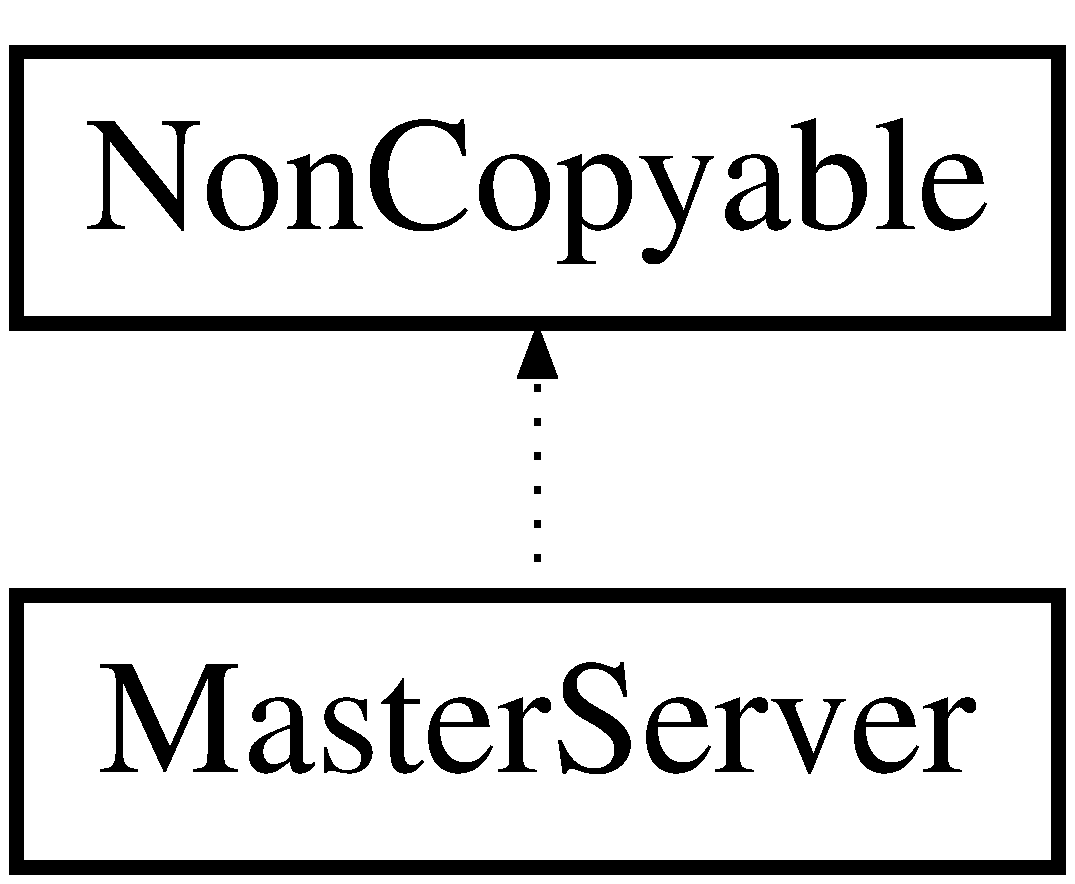
\includegraphics[height=2.000000cm]{class_master_server}
\end{center}
\end{figure}
\subsection*{Public Member Functions}
\begin{DoxyCompactItemize}
\item 
\hypertarget{class_master_server_a139dfe6cb90deb161e607aa982a8a801}{void {\bfseries run} ()}\label{class_master_server_a139dfe6cb90deb161e607aa982a8a801}

\item 
\hypertarget{class_master_server_aa26fde6f9d9ae3a1f7041175450532fa}{void {\bfseries build} ()}\label{class_master_server_aa26fde6f9d9ae3a1f7041175450532fa}

\end{DoxyCompactItemize}


The documentation for this class was generated from the following files\-:\begin{DoxyCompactItemize}
\item 
include/Master\-Server.\-hpp\item 
src/Master\-Server.\-cpp\end{DoxyCompactItemize}

\hypertarget{struct_mem}{\section{Mem Struct Reference}
\label{struct_mem}\index{Mem@{Mem}}
}
\subsection*{Public Attributes}
\begin{DoxyCompactItemize}
\item 
\hypertarget{struct_mem_a478da33d1e83a23931b372f9ddc706f2}{\hyperlink{structsqlite3}{sqlite3} $\ast$ {\bfseries db}}\label{struct_mem_a478da33d1e83a23931b372f9ddc706f2}

\item 
\hypertarget{struct_mem_a85c51a0b445063ba913693517860f5ea}{char $\ast$ {\bfseries z}}\label{struct_mem_a85c51a0b445063ba913693517860f5ea}

\item 
\hypertarget{struct_mem_a89ce926e95eb6d3f75344fd6525229da}{double {\bfseries r}}\label{struct_mem_a89ce926e95eb6d3f75344fd6525229da}

\item 
\hypertarget{struct_mem_a99e10893cbe980a11f045768beb20650}{\begin{tabbing}
xx\=xx\=xx\=xx\=xx\=xx\=xx\=xx\=xx\=\kill
union \{\\
\>i64 {\bfseries i}\\
\>int {\bfseries nZero}\\
\>\hyperlink{struct_func_def}{FuncDef} $\ast$ {\bfseries pDef}\\
\>\hyperlink{struct_row_set}{RowSet} $\ast$ {\bfseries pRowSet}\\
\>\hyperlink{struct_vdbe_frame}{VdbeFrame} $\ast$ {\bfseries pFrame}\\
\} {\bfseries u}}\label{struct_mem_a99e10893cbe980a11f045768beb20650}
\\

\end{tabbing}\item 
\hypertarget{struct_mem_a5a613756e096c221ec68077c28424d84}{int {\bfseries n}}\label{struct_mem_a5a613756e096c221ec68077c28424d84}

\item 
\hypertarget{struct_mem_a209bf3317161d1e33af9fe8b512f4974}{u16 {\bfseries flags}}\label{struct_mem_a209bf3317161d1e33af9fe8b512f4974}

\item 
\hypertarget{struct_mem_a6756879ca1e5fa71b12db25f981b7e87}{u8 {\bfseries type}}\label{struct_mem_a6756879ca1e5fa71b12db25f981b7e87}

\item 
\hypertarget{struct_mem_af437c99e92b8e729b70f82fa94e96bff}{u8 {\bfseries enc}}\label{struct_mem_af437c99e92b8e729b70f82fa94e96bff}

\item 
\hypertarget{struct_mem_a081ea2f86933d68a8940785b62f638ef}{void($\ast$ {\bfseries x\-Del} )(void $\ast$)}\label{struct_mem_a081ea2f86933d68a8940785b62f638ef}

\item 
\hypertarget{struct_mem_a68cd8f196d9dc8ab27845e1b4abbc95c}{char $\ast$ {\bfseries z\-Malloc}}\label{struct_mem_a68cd8f196d9dc8ab27845e1b4abbc95c}

\end{DoxyCompactItemize}


The documentation for this struct was generated from the following file\-:\begin{DoxyCompactItemize}
\item 
src/sqlite3.\-c\end{DoxyCompactItemize}

\hypertarget{struct_mem_journal}{\section{Mem\-Journal Struct Reference}
\label{struct_mem_journal}\index{Mem\-Journal@{Mem\-Journal}}
}
\subsection*{Public Attributes}
\begin{DoxyCompactItemize}
\item 
\hypertarget{struct_mem_journal_a00c1523cce1bcfadc2b672b8703a78cb}{\hyperlink{structsqlite3__io__methods}{sqlite3\-\_\-io\-\_\-methods} $\ast$ {\bfseries p\-Method}}\label{struct_mem_journal_a00c1523cce1bcfadc2b672b8703a78cb}

\item 
\hypertarget{struct_mem_journal_ade7a6dea7b38a8a86f33476ae207765f}{\hyperlink{struct_file_chunk}{File\-Chunk} $\ast$ {\bfseries p\-First}}\label{struct_mem_journal_ade7a6dea7b38a8a86f33476ae207765f}

\item 
\hypertarget{struct_mem_journal_ac69637f95cfbce175cbeef00f71e59a9}{\hyperlink{struct_file_point}{File\-Point} {\bfseries endpoint}}\label{struct_mem_journal_ac69637f95cfbce175cbeef00f71e59a9}

\item 
\hypertarget{struct_mem_journal_a5645d38e1a488b62b5f63112628bf472}{\hyperlink{struct_file_point}{File\-Point} {\bfseries readpoint}}\label{struct_mem_journal_a5645d38e1a488b62b5f63112628bf472}

\end{DoxyCompactItemize}


The documentation for this struct was generated from the following file\-:\begin{DoxyCompactItemize}
\item 
src/sqlite3.\-c\end{DoxyCompactItemize}

\hypertarget{struct_mem_page}{\section{Mem\-Page Struct Reference}
\label{struct_mem_page}\index{Mem\-Page@{Mem\-Page}}
}
\subsection*{Public Attributes}
\begin{DoxyCompactItemize}
\item 
\hypertarget{struct_mem_page_a3ab4ace46245be0fb2fb19eaa2862019}{u8 {\bfseries is\-Init}}\label{struct_mem_page_a3ab4ace46245be0fb2fb19eaa2862019}

\item 
\hypertarget{struct_mem_page_a3f7fa1a1eba3af840ef887e8ddd6d2cc}{u8 {\bfseries n\-Overflow}}\label{struct_mem_page_a3f7fa1a1eba3af840ef887e8ddd6d2cc}

\item 
\hypertarget{struct_mem_page_a46784c3c4708c7a582cff81a29c55323}{u8 {\bfseries int\-Key}}\label{struct_mem_page_a46784c3c4708c7a582cff81a29c55323}

\item 
\hypertarget{struct_mem_page_af18504bd0a2e7d39d9b485d434af0447}{u8 {\bfseries leaf}}\label{struct_mem_page_af18504bd0a2e7d39d9b485d434af0447}

\item 
\hypertarget{struct_mem_page_af7b608d25c2e326f82cc270cd53dd8f8}{u8 {\bfseries has\-Data}}\label{struct_mem_page_af7b608d25c2e326f82cc270cd53dd8f8}

\item 
\hypertarget{struct_mem_page_a01967a1a593980fb71c8ccf3393ae156}{u8 {\bfseries hdr\-Offset}}\label{struct_mem_page_a01967a1a593980fb71c8ccf3393ae156}

\item 
\hypertarget{struct_mem_page_aeba10281fc255d9bbc0e31486f8fbd48}{u8 {\bfseries child\-Ptr\-Size}}\label{struct_mem_page_aeba10281fc255d9bbc0e31486f8fbd48}

\item 
\hypertarget{struct_mem_page_a79548547cafb0e6d8549006bdc553f0a}{u8 {\bfseries max1byte\-Payload}}\label{struct_mem_page_a79548547cafb0e6d8549006bdc553f0a}

\item 
\hypertarget{struct_mem_page_a36394b7c3abf4652e7a24be4ab314f13}{u16 {\bfseries max\-Local}}\label{struct_mem_page_a36394b7c3abf4652e7a24be4ab314f13}

\item 
\hypertarget{struct_mem_page_a95cab31aa57bf8b478be273557c5c807}{u16 {\bfseries min\-Local}}\label{struct_mem_page_a95cab31aa57bf8b478be273557c5c807}

\item 
\hypertarget{struct_mem_page_a324ed834d93c3ae72994fb5730940521}{u16 {\bfseries cell\-Offset}}\label{struct_mem_page_a324ed834d93c3ae72994fb5730940521}

\item 
\hypertarget{struct_mem_page_a3418a9aee707f57a73d8470f8a1228a8}{u16 {\bfseries n\-Free}}\label{struct_mem_page_a3418a9aee707f57a73d8470f8a1228a8}

\item 
\hypertarget{struct_mem_page_a35d1d8f836201b82b1eb778ce0e324f4}{u16 {\bfseries n\-Cell}}\label{struct_mem_page_a35d1d8f836201b82b1eb778ce0e324f4}

\item 
\hypertarget{struct_mem_page_aa3d64e8755cc9f431bbc8423a2b506ec}{u16 {\bfseries mask\-Page}}\label{struct_mem_page_aa3d64e8755cc9f431bbc8423a2b506ec}

\item 
\hypertarget{struct_mem_page_a857e00533053fe6017c6e08b1b240661}{u16 {\bfseries ai\-Ovfl} \mbox{[}5\mbox{]}}\label{struct_mem_page_a857e00533053fe6017c6e08b1b240661}

\item 
\hypertarget{struct_mem_page_a3a6347d06b1e85938605d9a44f193cb9}{u8 $\ast$ {\bfseries ap\-Ovfl} \mbox{[}5\mbox{]}}\label{struct_mem_page_a3a6347d06b1e85938605d9a44f193cb9}

\item 
\hypertarget{struct_mem_page_a949df1156f7392592eaeb64389068f99}{\hyperlink{struct_bt_shared}{Bt\-Shared} $\ast$ {\bfseries p\-Bt}}\label{struct_mem_page_a949df1156f7392592eaeb64389068f99}

\item 
\hypertarget{struct_mem_page_a2d873eff563d2208be0c24959140a4b0}{u8 $\ast$ {\bfseries a\-Data}}\label{struct_mem_page_a2d873eff563d2208be0c24959140a4b0}

\item 
\hypertarget{struct_mem_page_ab5d2ecb95a84eaf4bd0ccef536bac6d7}{u8 $\ast$ {\bfseries a\-Data\-End}}\label{struct_mem_page_ab5d2ecb95a84eaf4bd0ccef536bac6d7}

\item 
\hypertarget{struct_mem_page_a6f391f110e68ede6e5234b4e9f678f99}{u8 $\ast$ {\bfseries a\-Cell\-Idx}}\label{struct_mem_page_a6f391f110e68ede6e5234b4e9f678f99}

\item 
\hypertarget{struct_mem_page_add322c1aed91e95d8dfe3ac3535d65b4}{\hyperlink{struct_pg_hdr}{Db\-Page} $\ast$ {\bfseries p\-Db\-Page}}\label{struct_mem_page_add322c1aed91e95d8dfe3ac3535d65b4}

\item 
\hypertarget{struct_mem_page_ad2b0c532abc799bbcf3b43df4f0b0546}{Pgno {\bfseries pgno}}\label{struct_mem_page_ad2b0c532abc799bbcf3b43df4f0b0546}

\end{DoxyCompactItemize}


The documentation for this struct was generated from the following file\-:\begin{DoxyCompactItemize}
\item 
src/sqlite3.\-c\end{DoxyCompactItemize}

\hypertarget{struct_module}{\section{Module Struct Reference}
\label{struct_module}\index{Module@{Module}}
}
\subsection*{Public Attributes}
\begin{DoxyCompactItemize}
\item 
\hypertarget{struct_module_a65d2539d71ea028b505b2fb33563bfd7}{const \hyperlink{structsqlite3__module}{sqlite3\-\_\-module} $\ast$ {\bfseries p\-Module}}\label{struct_module_a65d2539d71ea028b505b2fb33563bfd7}

\item 
\hypertarget{struct_module_a45a5f5b43926b8ebf3e13e46a6534810}{const char $\ast$ {\bfseries z\-Name}}\label{struct_module_a45a5f5b43926b8ebf3e13e46a6534810}

\item 
\hypertarget{struct_module_ae3b827fee4c8b4f3ff38c86c2e2f48cd}{void $\ast$ {\bfseries p\-Aux}}\label{struct_module_ae3b827fee4c8b4f3ff38c86c2e2f48cd}

\item 
\hypertarget{struct_module_a4be509110a1a2f2c06a5d69af45704ca}{void($\ast$ {\bfseries x\-Destroy} )(void $\ast$)}\label{struct_module_a4be509110a1a2f2c06a5d69af45704ca}

\end{DoxyCompactItemize}


The documentation for this struct was generated from the following file\-:\begin{DoxyCompactItemize}
\item 
src/sqlite3.\-c\end{DoxyCompactItemize}

\hypertarget{class_mutexes}{\section{Mutexes Class Reference}
\label{class_mutexes}\index{Mutexes@{Mutexes}}
}
\subsection*{Static Public Attributes}
\begin{DoxyCompactItemize}
\item 
\hypertarget{class_mutexes_a4ecb3dbaf0f590b2d8ba42cec64fdd93}{static sf\-::\-Mutex {\bfseries stdcout}}\label{class_mutexes_a4ecb3dbaf0f590b2d8ba42cec64fdd93}

\item 
\hypertarget{class_mutexes_ad263e2d0b12f337beacbc53ffd69905b}{static sf\-::\-Mutex {\bfseries messages}}\label{class_mutexes_ad263e2d0b12f337beacbc53ffd69905b}

\end{DoxyCompactItemize}


The documentation for this class was generated from the following files\-:\begin{DoxyCompactItemize}
\item 
include/Mutexes.\-hpp\item 
src/Mutexes.\-cpp\end{DoxyCompactItemize}

\hypertarget{struct_name_context}{\section{Name\-Context Struct Reference}
\label{struct_name_context}\index{Name\-Context@{Name\-Context}}
}
\subsection*{Public Attributes}
\begin{DoxyCompactItemize}
\item 
\hypertarget{struct_name_context_a14635249bf75d5e18124089571dd2386}{\hyperlink{struct_parse}{Parse} $\ast$ {\bfseries p\-Parse}}\label{struct_name_context_a14635249bf75d5e18124089571dd2386}

\item 
\hypertarget{struct_name_context_a6ede21da33e2e9bd3d0c5fe90a3ec72c}{\hyperlink{struct_src_list}{Src\-List} $\ast$ {\bfseries p\-Src\-List}}\label{struct_name_context_a6ede21da33e2e9bd3d0c5fe90a3ec72c}

\item 
\hypertarget{struct_name_context_a8c752d7fb9b28179156c569cc57ba6f2}{\hyperlink{struct_expr_list}{Expr\-List} $\ast$ {\bfseries p\-E\-List}}\label{struct_name_context_a8c752d7fb9b28179156c569cc57ba6f2}

\item 
\hypertarget{struct_name_context_aeb3ff72c03dd770d421cadc2195a5644}{\hyperlink{struct_agg_info}{Agg\-Info} $\ast$ {\bfseries p\-Agg\-Info}}\label{struct_name_context_aeb3ff72c03dd770d421cadc2195a5644}

\item 
\hypertarget{struct_name_context_a82ce0ec8a3cc3d792e1f38bb5e0ad5fc}{\hyperlink{struct_name_context}{Name\-Context} $\ast$ {\bfseries p\-Next}}\label{struct_name_context_a82ce0ec8a3cc3d792e1f38bb5e0ad5fc}

\item 
\hypertarget{struct_name_context_ad68616ce2a58fa1b135e0dcf953bdc97}{int {\bfseries n\-Ref}}\label{struct_name_context_ad68616ce2a58fa1b135e0dcf953bdc97}

\item 
\hypertarget{struct_name_context_aba0b89b42e945c4c96d57a8fe011329c}{int {\bfseries n\-Err}}\label{struct_name_context_aba0b89b42e945c4c96d57a8fe011329c}

\item 
\hypertarget{struct_name_context_a3dcc2e5442b6a74440a15226139b78d2}{u8 {\bfseries nc\-Flags}}\label{struct_name_context_a3dcc2e5442b6a74440a15226139b78d2}

\end{DoxyCompactItemize}


The documentation for this struct was generated from the following file\-:\begin{DoxyCompactItemize}
\item 
src/sqlite3.\-c\end{DoxyCompactItemize}

\hypertarget{class_networked_character}{\section{Networked\-Character Class Reference}
\label{class_networked_character}\index{Networked\-Character@{Networked\-Character}}
}
Inheritance diagram for Networked\-Character\-:\begin{figure}[H]
\begin{center}
\leavevmode
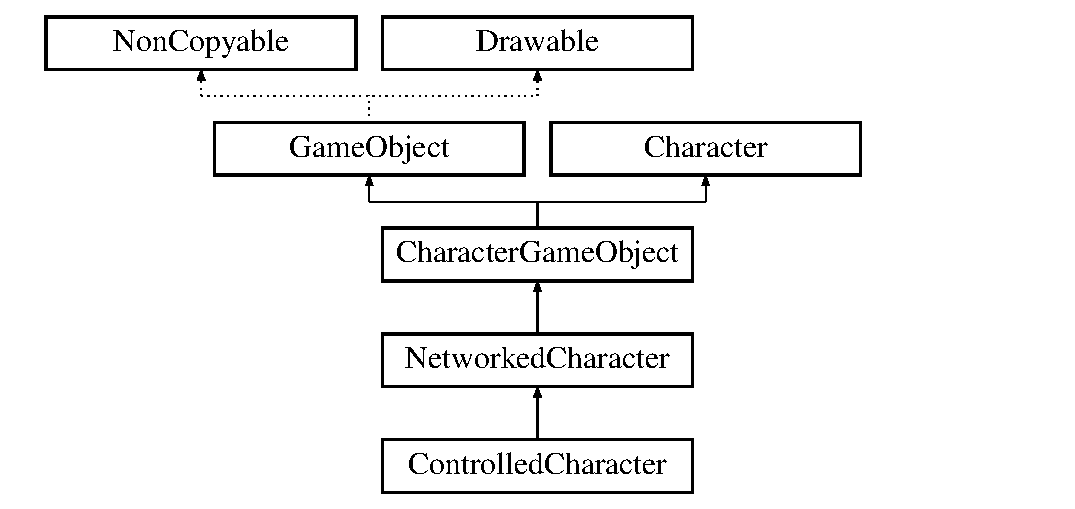
\includegraphics[height=5.000000cm]{class_networked_character}
\end{center}
\end{figure}
\subsection*{Public Member Functions}
\begin{DoxyCompactItemize}
\item 
\hypertarget{class_networked_character_a8186d89a0b00c184d66e9cbdee07a4f0}{{\bfseries Networked\-Character} (const std\-::string \&, const sf\-::\-Color \&)}\label{class_networked_character_a8186d89a0b00c184d66e9cbdee07a4f0}

\end{DoxyCompactItemize}
\subsection*{Public Attributes}
\begin{DoxyCompactItemize}
\item 
\hypertarget{class_networked_character_a459f88e77a2085a507507f7760408cf6}{\hyperlink{class_key_state}{Key\-State} {\bfseries key\-State}}\label{class_networked_character_a459f88e77a2085a507507f7760408cf6}

\end{DoxyCompactItemize}
\subsection*{Protected Member Functions}
\begin{DoxyCompactItemize}
\item 
\hypertarget{class_networked_character_af8a7f21f2195d8d789fa61ccca88ccfa}{virtual void {\bfseries update} ()}\label{class_networked_character_af8a7f21f2195d8d789fa61ccca88ccfa}

\end{DoxyCompactItemize}
\subsection*{Additional Inherited Members}


The documentation for this class was generated from the following files\-:\begin{DoxyCompactItemize}
\item 
include/Networked\-Character.\-hpp\item 
src/Networked\-Character.\-cpp\end{DoxyCompactItemize}

\hypertarget{class_network_event}{\section{Network\-Event Class Reference}
\label{class_network_event}\index{Network\-Event@{Network\-Event}}
}
Inheritance diagram for Network\-Event\-:\begin{figure}[H]
\begin{center}
\leavevmode
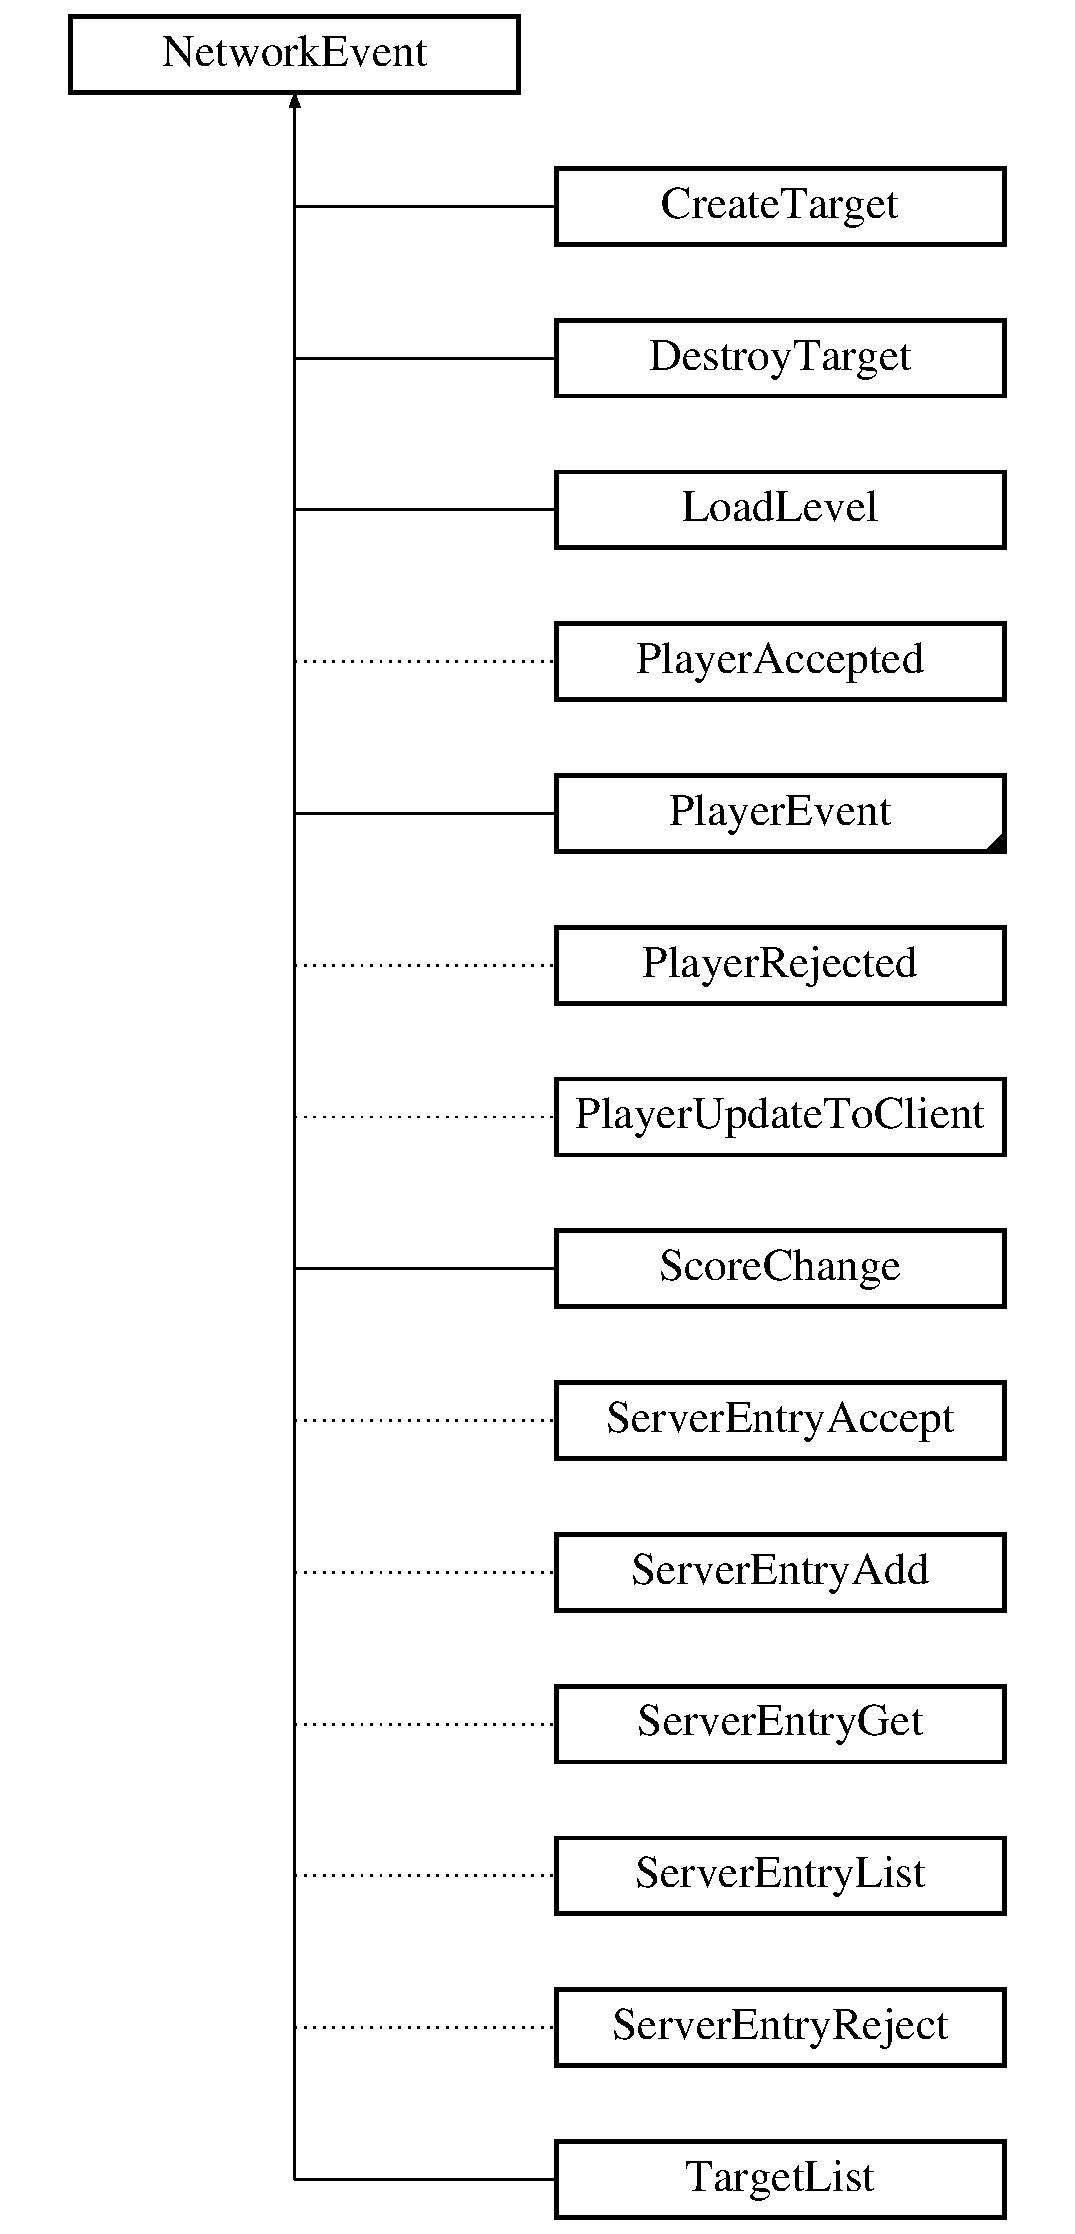
\includegraphics[height=12.000000cm]{class_network_event}
\end{center}
\end{figure}
\subsection*{Public Types}
\begin{DoxyCompactItemize}
\item 
enum {\bfseries Commands} \{ \\*
{\bfseries P\-L\-A\-Y\-E\-R\-\_\-\-C\-O\-N\-N\-E\-C\-T\-E\-D}, 
{\bfseries P\-L\-A\-Y\-E\-R\-\_\-\-A\-U\-T\-H\-O\-R\-I\-Z\-E}, 
{\bfseries P\-L\-A\-Y\-E\-R\-\_\-\-D\-I\-S\-C\-O\-N\-N\-E\-C\-T\-E\-D}, 
{\bfseries P\-L\-A\-Y\-E\-R\-\_\-\-S\-E\-N\-D\-\_\-\-M\-E\-S\-S\-A\-G\-E}, 
\\*
{\bfseries P\-L\-A\-Y\-E\-R\-\_\-\-R\-E\-J\-E\-C\-T\-E\-D}, 
{\bfseries P\-L\-A\-Y\-E\-R\-\_\-\-A\-C\-C\-E\-P\-T\-E\-D}, 
{\bfseries P\-L\-A\-Y\-E\-R\-\_\-\-U\-P\-D\-A\-T\-E\-\_\-\-T\-O\-\_\-\-S\-E\-R\-V\-E\-R}, 
{\bfseries P\-L\-A\-Y\-E\-R\-\_\-\-U\-P\-D\-A\-T\-E\-\_\-\-T\-O\-\_\-\-C\-L\-I\-E\-N\-T}, 
\\*
{\bfseries S\-E\-R\-V\-E\-R\-\_\-\-E\-N\-T\-R\-Y\-\_\-\-G\-E\-T}, 
{\bfseries S\-E\-R\-V\-E\-R\-\_\-\-E\-N\-T\-R\-Y\-\_\-\-A\-D\-D}, 
{\bfseries S\-E\-R\-V\-E\-R\-\_\-\-E\-N\-T\-R\-Y\-\_\-\-L\-I\-S\-T}, 
{\bfseries S\-E\-R\-V\-E\-R\-\_\-\-E\-N\-T\-R\-Y\-\_\-\-A\-C\-C\-E\-P\-T}, 
\\*
{\bfseries S\-E\-R\-V\-E\-R\-\_\-\-E\-N\-T\-R\-Y\-\_\-\-R\-E\-J\-E\-C\-T}, 
{\bfseries L\-O\-A\-D\-\_\-\-L\-E\-V\-E\-L}, 
{\bfseries C\-R\-E\-A\-T\-E\-\_\-\-T\-A\-R\-G\-E\-T}, 
{\bfseries D\-E\-S\-T\-R\-O\-Y\-\_\-\-T\-A\-R\-G\-E\-T}, 
\\*
{\bfseries T\-A\-R\-G\-E\-T\-\_\-\-L\-I\-S\-T}, 
{\bfseries S\-C\-O\-R\-E\-\_\-\-C\-H\-A\-N\-G\-E}
 \}
\end{DoxyCompactItemize}
\subsection*{Public Member Functions}
\begin{DoxyCompactItemize}
\item 
\hypertarget{class_network_event_a6148b15dfb7bc081628d2c0a73fd7751}{virtual sf\-::\-Int32 {\bfseries get\-Command} () const =0}\label{class_network_event_a6148b15dfb7bc081628d2c0a73fd7751}

\end{DoxyCompactItemize}


The documentation for this class was generated from the following file\-:\begin{DoxyCompactItemize}
\item 
include/Network\-Events.\-h\end{DoxyCompactItemize}

\hypertarget{class_network_interface}{\section{Network\-Interface Class Reference}
\label{class_network_interface}\index{Network\-Interface@{Network\-Interface}}
}


{\ttfamily \#include $<$Network\-Interface.\-hpp$>$}

Inheritance diagram for Network\-Interface\-:\begin{figure}[H]
\begin{center}
\leavevmode
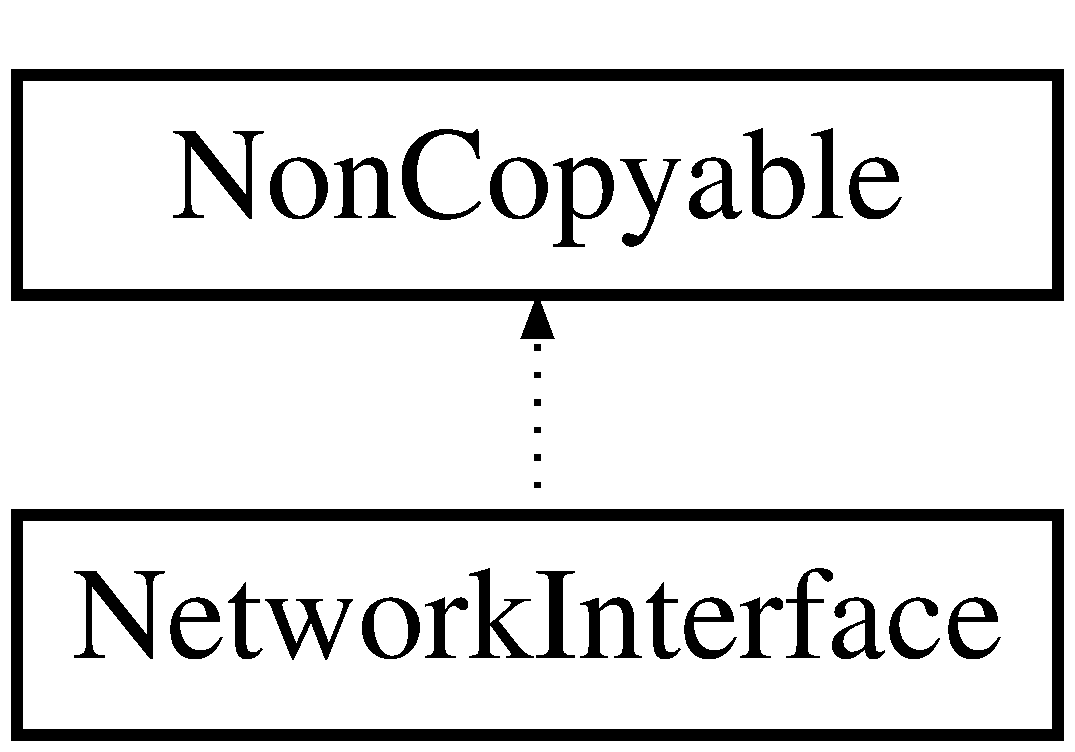
\includegraphics[height=2.000000cm]{class_network_interface}
\end{center}
\end{figure}
\subsection*{Public Member Functions}
\begin{DoxyCompactItemize}
\item 
virtual \hyperlink{class_network_interface_adc72badb87b206431e240704e9aaa7c1}{$\sim$\-Network\-Interface} ()
\item 
bool \hyperlink{class_network_interface_addb6ab95cd5650952ac96270dc93c584}{connect\-To\-Ip} (const sf\-::\-Ip\-Address \&ip)
\item 
void \hyperlink{class_network_interface_a56f56d384eb1c6467e9b06d8e6b0b270}{disconnect\-From\-Server} ()
\item 
void \hyperlink{class_network_interface_a3589d7035ab5b0811a4026717dddc4a8}{handle\-Messages} (\hyperlink{class_game}{Game} \&game)
\item 
void \hyperlink{class_network_interface_a911ec8a94345995c2a9b8de593d65449}{ask\-For\-Server\-List} ()
\item 
\hypertarget{class_network_interface_af6129658a71407335a3db9ce15946893}{void {\bfseries send\-State\-Update} ()}\label{class_network_interface_af6129658a71407335a3db9ce15946893}

\item 
\hypertarget{class_network_interface_aae98c4b2b4d994f8eb20ae2c319b5b8a}{bool {\bfseries get\-Connected} () const }\label{class_network_interface_aae98c4b2b4d994f8eb20ae2c319b5b8a}

\item 
\hypertarget{class_network_interface_ae7761124af88949f00d0c209a11c2384}{void {\bfseries send\-Authorize\-Message} ()}\label{class_network_interface_ae7761124af88949f00d0c209a11c2384}

\end{DoxyCompactItemize}


\subsection{Detailed Description}
Handles network operatations that the game requires it to do 

\subsection{Constructor \& Destructor Documentation}
\hypertarget{class_network_interface_adc72badb87b206431e240704e9aaa7c1}{\index{Network\-Interface@{Network\-Interface}!$\sim$\-Network\-Interface@{$\sim$\-Network\-Interface}}
\index{$\sim$\-Network\-Interface@{$\sim$\-Network\-Interface}!NetworkInterface@{Network\-Interface}}
\subsubsection[{$\sim$\-Network\-Interface}]{\setlength{\rightskip}{0pt plus 5cm}Network\-Interface\-::$\sim$\-Network\-Interface (
\begin{DoxyParamCaption}
{}
\end{DoxyParamCaption}
)\hspace{0.3cm}{\ttfamily [virtual]}}}\label{class_network_interface_adc72badb87b206431e240704e9aaa7c1}
Connect tcp socket to specified ip 

\subsection{Member Function Documentation}
\hypertarget{class_network_interface_a911ec8a94345995c2a9b8de593d65449}{\index{Network\-Interface@{Network\-Interface}!ask\-For\-Server\-List@{ask\-For\-Server\-List}}
\index{ask\-For\-Server\-List@{ask\-For\-Server\-List}!NetworkInterface@{Network\-Interface}}
\subsubsection[{ask\-For\-Server\-List}]{\setlength{\rightskip}{0pt plus 5cm}void Network\-Interface\-::ask\-For\-Server\-List (
\begin{DoxyParamCaption}
{}
\end{DoxyParamCaption}
)}}\label{class_network_interface_a911ec8a94345995c2a9b8de593d65449}
Send state of player over to the server \hypertarget{class_network_interface_addb6ab95cd5650952ac96270dc93c584}{\index{Network\-Interface@{Network\-Interface}!connect\-To\-Ip@{connect\-To\-Ip}}
\index{connect\-To\-Ip@{connect\-To\-Ip}!NetworkInterface@{Network\-Interface}}
\subsubsection[{connect\-To\-Ip}]{\setlength{\rightskip}{0pt plus 5cm}bool Network\-Interface\-::connect\-To\-Ip (
\begin{DoxyParamCaption}
\item[{const sf\-::\-Ip\-Address \&}]{ip}
\end{DoxyParamCaption}
)}}\label{class_network_interface_addb6ab95cd5650952ac96270dc93c584}
Send the server that we are connected to a message that we are about to disconnect \hypertarget{class_network_interface_a56f56d384eb1c6467e9b06d8e6b0b270}{\index{Network\-Interface@{Network\-Interface}!disconnect\-From\-Server@{disconnect\-From\-Server}}
\index{disconnect\-From\-Server@{disconnect\-From\-Server}!NetworkInterface@{Network\-Interface}}
\subsubsection[{disconnect\-From\-Server}]{\setlength{\rightskip}{0pt plus 5cm}void Network\-Interface\-::disconnect\-From\-Server (
\begin{DoxyParamCaption}
{}
\end{DoxyParamCaption}
)}}\label{class_network_interface_a56f56d384eb1c6467e9b06d8e6b0b270}
Calls hangle\-Message in the game class for each packet that has to be processed. \hypertarget{class_network_interface_a3589d7035ab5b0811a4026717dddc4a8}{\index{Network\-Interface@{Network\-Interface}!handle\-Messages@{handle\-Messages}}
\index{handle\-Messages@{handle\-Messages}!NetworkInterface@{Network\-Interface}}
\subsubsection[{handle\-Messages}]{\setlength{\rightskip}{0pt plus 5cm}void Network\-Interface\-::handle\-Messages (
\begin{DoxyParamCaption}
\item[{{\bf Game} \&}]{game}
\end{DoxyParamCaption}
)}}\label{class_network_interface_a3589d7035ab5b0811a4026717dddc4a8}
Ask the master server to send a server list to this client 

The documentation for this class was generated from the following files\-:\begin{DoxyCompactItemize}
\item 
include/Network\-Interface.\-hpp\item 
src/Network\-Interface.\-cpp\end{DoxyCompactItemize}

\hypertarget{struct_packet_wrap}{\section{Packet\-Wrap Struct Reference}
\label{struct_packet_wrap}\index{Packet\-Wrap@{Packet\-Wrap}}
}
\subsection*{Public Member Functions}
\begin{DoxyCompactItemize}
\item 
\hypertarget{struct_packet_wrap_a848a1388a9c753487fc4d2805b400b70}{{\bfseries Packet\-Wrap} (const sf\-::\-Packet \&pack, const sf\-::\-Ip\-Address \&ip, unsigned short port)}\label{struct_packet_wrap_a848a1388a9c753487fc4d2805b400b70}

\end{DoxyCompactItemize}
\subsection*{Public Attributes}
\begin{DoxyCompactItemize}
\item 
\hypertarget{struct_packet_wrap_a1aa4f42a3a2506316a4580ade8b0be5a}{sf\-::\-Packet {\bfseries packet}}\label{struct_packet_wrap_a1aa4f42a3a2506316a4580ade8b0be5a}

\item 
\hypertarget{struct_packet_wrap_aee7440a6f2cf105f27e084a6d95928f3}{sf\-::\-Ip\-Address {\bfseries from\-Ip}}\label{struct_packet_wrap_aee7440a6f2cf105f27e084a6d95928f3}

\item 
\hypertarget{struct_packet_wrap_a687da347d509e1105f0ee578704a188e}{unsigned short {\bfseries from\-Port}}\label{struct_packet_wrap_a687da347d509e1105f0ee578704a188e}

\end{DoxyCompactItemize}


The documentation for this struct was generated from the following file\-:\begin{DoxyCompactItemize}
\item 
include/Network\-Events.\-h\end{DoxyCompactItemize}

\hypertarget{struct_pager}{\section{Pager Struct Reference}
\label{struct_pager}\index{Pager@{Pager}}
}
\subsection*{Public Attributes}
\begin{DoxyCompactItemize}
\item 
\hypertarget{struct_pager_affa78e08a7f691a4c8f7043e0b4c9212}{\hyperlink{structsqlite3__vfs}{sqlite3\-\_\-vfs} $\ast$ {\bfseries p\-Vfs}}\label{struct_pager_affa78e08a7f691a4c8f7043e0b4c9212}

\item 
\hypertarget{struct_pager_a5cbccc156e07d6226cb65a7ab05ac116}{u8 {\bfseries exclusive\-Mode}}\label{struct_pager_a5cbccc156e07d6226cb65a7ab05ac116}

\item 
\hypertarget{struct_pager_a9ad7bd09f1c9323d943ee17ddf42e46e}{u8 {\bfseries journal\-Mode}}\label{struct_pager_a9ad7bd09f1c9323d943ee17ddf42e46e}

\item 
\hypertarget{struct_pager_af7783f866150d7e322c28cb324ad85d6}{u8 {\bfseries use\-Journal}}\label{struct_pager_af7783f866150d7e322c28cb324ad85d6}

\item 
\hypertarget{struct_pager_ae943093a3ccbfbf264ccf3c8a52edac1}{u8 {\bfseries no\-Sync}}\label{struct_pager_ae943093a3ccbfbf264ccf3c8a52edac1}

\item 
\hypertarget{struct_pager_abae5c9c3d85120ae266acc4c9a355b86}{u8 {\bfseries full\-Sync}}\label{struct_pager_abae5c9c3d85120ae266acc4c9a355b86}

\item 
\hypertarget{struct_pager_a4543ec92953e7bda49b3ed4f0bdab890}{u8 {\bfseries ckpt\-Sync\-Flags}}\label{struct_pager_a4543ec92953e7bda49b3ed4f0bdab890}

\item 
\hypertarget{struct_pager_aa8c8c2d893e4d2165f089ddde3e85103}{u8 {\bfseries wal\-Sync\-Flags}}\label{struct_pager_aa8c8c2d893e4d2165f089ddde3e85103}

\item 
\hypertarget{struct_pager_ac7f90d27da63090369a0e44a0bceb525}{u8 {\bfseries sync\-Flags}}\label{struct_pager_ac7f90d27da63090369a0e44a0bceb525}

\item 
\hypertarget{struct_pager_a9caa1abb43f6e839dd9a265c27b0b9e4}{u8 {\bfseries temp\-File}}\label{struct_pager_a9caa1abb43f6e839dd9a265c27b0b9e4}

\item 
\hypertarget{struct_pager_ad7a7013309fd80a2a01844e69e8e7398}{u8 {\bfseries read\-Only}}\label{struct_pager_ad7a7013309fd80a2a01844e69e8e7398}

\item 
\hypertarget{struct_pager_abca3633b7745075aa5cf432b3fae54f2}{u8 {\bfseries mem\-Db}}\label{struct_pager_abca3633b7745075aa5cf432b3fae54f2}

\item 
\hypertarget{struct_pager_af03ee0ac77cf73453295ffcf43e46b43}{u8 {\bfseries e\-State}}\label{struct_pager_af03ee0ac77cf73453295ffcf43e46b43}

\item 
\hypertarget{struct_pager_afcaf60e4b0be0995c926e3357d4bbef0}{u8 {\bfseries e\-Lock}}\label{struct_pager_afcaf60e4b0be0995c926e3357d4bbef0}

\item 
\hypertarget{struct_pager_a90c86a51ec6805d5702d32e456b0bcdc}{u8 {\bfseries change\-Count\-Done}}\label{struct_pager_a90c86a51ec6805d5702d32e456b0bcdc}

\item 
\hypertarget{struct_pager_acd7eae0587c98ac41afab04e4b5defcb}{u8 {\bfseries set\-Master}}\label{struct_pager_acd7eae0587c98ac41afab04e4b5defcb}

\item 
\hypertarget{struct_pager_a2f6579b3006b692a4ce1e5ad3e9a58ed}{u8 {\bfseries do\-Not\-Spill}}\label{struct_pager_a2f6579b3006b692a4ce1e5ad3e9a58ed}

\item 
\hypertarget{struct_pager_a227d91995648a4e730d2adecc3533dba}{u8 {\bfseries do\-Not\-Sync\-Spill}}\label{struct_pager_a227d91995648a4e730d2adecc3533dba}

\item 
\hypertarget{struct_pager_a9205654b516184d84fde5c3b5f72ff77}{u8 {\bfseries subj\-In\-Memory}}\label{struct_pager_a9205654b516184d84fde5c3b5f72ff77}

\item 
\hypertarget{struct_pager_afa5d7849190ef0a9a6f85bb15f2444b3}{Pgno {\bfseries db\-Size}}\label{struct_pager_afa5d7849190ef0a9a6f85bb15f2444b3}

\item 
\hypertarget{struct_pager_a8f9cd11d6ae3fac48182e6eae0810c6a}{Pgno {\bfseries db\-Orig\-Size}}\label{struct_pager_a8f9cd11d6ae3fac48182e6eae0810c6a}

\item 
\hypertarget{struct_pager_a1f8f55f49cb0ec91bfde4dca96a13f13}{Pgno {\bfseries db\-File\-Size}}\label{struct_pager_a1f8f55f49cb0ec91bfde4dca96a13f13}

\item 
\hypertarget{struct_pager_aa99d74d10ef3cdcf61501f9777a0246b}{Pgno {\bfseries db\-Hint\-Size}}\label{struct_pager_aa99d74d10ef3cdcf61501f9777a0246b}

\item 
\hypertarget{struct_pager_addaf9648a1111d7b6c85166cf7c7a575}{int {\bfseries err\-Code}}\label{struct_pager_addaf9648a1111d7b6c85166cf7c7a575}

\item 
\hypertarget{struct_pager_a3a202368c065a43695533503c98f28d9}{int {\bfseries n\-Rec}}\label{struct_pager_a3a202368c065a43695533503c98f28d9}

\item 
\hypertarget{struct_pager_ad799667658328a44b471378a1b99623e}{u32 {\bfseries cksum\-Init}}\label{struct_pager_ad799667658328a44b471378a1b99623e}

\item 
\hypertarget{struct_pager_a670c4c54515c0257c35ddfc07c43763e}{u32 {\bfseries n\-Sub\-Rec}}\label{struct_pager_a670c4c54515c0257c35ddfc07c43763e}

\item 
\hypertarget{struct_pager_a530ea868337a7c0c4e7c125035f73737}{\hyperlink{struct_bitvec}{Bitvec} $\ast$ {\bfseries p\-In\-Journal}}\label{struct_pager_a530ea868337a7c0c4e7c125035f73737}

\item 
\hypertarget{struct_pager_a005ff1960fc1550a870cd1dae418c99e}{\hyperlink{structsqlite3__file}{sqlite3\-\_\-file} $\ast$ {\bfseries fd}}\label{struct_pager_a005ff1960fc1550a870cd1dae418c99e}

\item 
\hypertarget{struct_pager_a81057c4420b8278e8141cf626abf4f0d}{\hyperlink{structsqlite3__file}{sqlite3\-\_\-file} $\ast$ {\bfseries jfd}}\label{struct_pager_a81057c4420b8278e8141cf626abf4f0d}

\item 
\hypertarget{struct_pager_a8196bcc97f184d480848895f71e080e6}{\hyperlink{structsqlite3__file}{sqlite3\-\_\-file} $\ast$ {\bfseries sjfd}}\label{struct_pager_a8196bcc97f184d480848895f71e080e6}

\item 
\hypertarget{struct_pager_ad3cffdc0987965fa6a472b19355f48df}{i64 {\bfseries journal\-Off}}\label{struct_pager_ad3cffdc0987965fa6a472b19355f48df}

\item 
\hypertarget{struct_pager_a7f4a7f5f0245b063a82c185f40bad7f0}{i64 {\bfseries journal\-Hdr}}\label{struct_pager_a7f4a7f5f0245b063a82c185f40bad7f0}

\item 
\hypertarget{struct_pager_ae230d34da61bf28178fa1ac142a88c15}{\hyperlink{structsqlite3__backup}{sqlite3\-\_\-backup} $\ast$ {\bfseries p\-Backup}}\label{struct_pager_ae230d34da61bf28178fa1ac142a88c15}

\item 
\hypertarget{struct_pager_a4d5f4487316c026eceb8461e90fffcfd}{\hyperlink{struct_pager_savepoint}{Pager\-Savepoint} $\ast$ {\bfseries a\-Savepoint}}\label{struct_pager_a4d5f4487316c026eceb8461e90fffcfd}

\item 
\hypertarget{struct_pager_a020adae89ef6c1b28e51fffc3d4b22c9}{int {\bfseries n\-Savepoint}}\label{struct_pager_a020adae89ef6c1b28e51fffc3d4b22c9}

\item 
\hypertarget{struct_pager_acf03a47838eee1cf474bb93dbc834b5f}{char {\bfseries db\-File\-Vers} \mbox{[}16\mbox{]}}\label{struct_pager_acf03a47838eee1cf474bb93dbc834b5f}

\item 
\hypertarget{struct_pager_a44e153b2f756bfb86ab471c25893b3b6}{u16 {\bfseries n\-Extra}}\label{struct_pager_a44e153b2f756bfb86ab471c25893b3b6}

\item 
\hypertarget{struct_pager_a82581087240713cab679108e3adeaf58}{i16 {\bfseries n\-Reserve}}\label{struct_pager_a82581087240713cab679108e3adeaf58}

\item 
\hypertarget{struct_pager_a36f3333fe82c70a46a99f2f8f289a971}{u32 {\bfseries vfs\-Flags}}\label{struct_pager_a36f3333fe82c70a46a99f2f8f289a971}

\item 
\hypertarget{struct_pager_a4a47c73d7c18b803df33ba6c39baa5bf}{u32 {\bfseries sector\-Size}}\label{struct_pager_a4a47c73d7c18b803df33ba6c39baa5bf}

\item 
\hypertarget{struct_pager_a9cfb910e7eaf8442f5414d722232a6e9}{int {\bfseries page\-Size}}\label{struct_pager_a9cfb910e7eaf8442f5414d722232a6e9}

\item 
\hypertarget{struct_pager_ad1d9a508ac764486a5eaef9b4f7781af}{Pgno {\bfseries mx\-Pgno}}\label{struct_pager_ad1d9a508ac764486a5eaef9b4f7781af}

\item 
\hypertarget{struct_pager_ae381db4e0b49f92596b0cdeb279e6bc6}{i64 {\bfseries journal\-Size\-Limit}}\label{struct_pager_ae381db4e0b49f92596b0cdeb279e6bc6}

\item 
\hypertarget{struct_pager_a2a55a044468f8658b7993e57087a5561}{char $\ast$ {\bfseries z\-Filename}}\label{struct_pager_a2a55a044468f8658b7993e57087a5561}

\item 
\hypertarget{struct_pager_ab36ce1f606c407ad3fc56a3651f5a319}{char $\ast$ {\bfseries z\-Journal}}\label{struct_pager_ab36ce1f606c407ad3fc56a3651f5a319}

\item 
\hypertarget{struct_pager_ac8477f7cc39fefd81b4089994e13d215}{int($\ast$ {\bfseries x\-Busy\-Handler} )(void $\ast$)}\label{struct_pager_ac8477f7cc39fefd81b4089994e13d215}

\item 
\hypertarget{struct_pager_a7a685e7a8dcbcd725c5a982fd8deb91b}{void $\ast$ {\bfseries p\-Busy\-Handler\-Arg}}\label{struct_pager_a7a685e7a8dcbcd725c5a982fd8deb91b}

\item 
\hypertarget{struct_pager_a0b3bb8afc7c4c82e0e99f3ad99dd0986}{int {\bfseries a\-Stat} \mbox{[}3\mbox{]}}\label{struct_pager_a0b3bb8afc7c4c82e0e99f3ad99dd0986}

\item 
\hypertarget{struct_pager_a632d3c81743a7f9104337ae3d45af04c}{void($\ast$ {\bfseries x\-Reiniter} )(\hyperlink{struct_pg_hdr}{Db\-Page} $\ast$)}\label{struct_pager_a632d3c81743a7f9104337ae3d45af04c}

\item 
\hypertarget{struct_pager_a64934188c72599e0be9ae54d3fc1cc92}{char $\ast$ {\bfseries p\-Tmp\-Space}}\label{struct_pager_a64934188c72599e0be9ae54d3fc1cc92}

\item 
\hypertarget{struct_pager_ae2495e45e354e92a858144386f91cab3}{\hyperlink{struct_p_cache}{P\-Cache} $\ast$ {\bfseries p\-P\-Cache}}\label{struct_pager_ae2495e45e354e92a858144386f91cab3}

\item 
\hypertarget{struct_pager_a2c759424108248d8b08e6f400fab14dd}{\hyperlink{struct_wal}{Wal} $\ast$ {\bfseries p\-Wal}}\label{struct_pager_a2c759424108248d8b08e6f400fab14dd}

\item 
\hypertarget{struct_pager_ac63ab281e48f9ac8521b85c1a90475b3}{char $\ast$ {\bfseries z\-Wal}}\label{struct_pager_ac63ab281e48f9ac8521b85c1a90475b3}

\end{DoxyCompactItemize}


The documentation for this struct was generated from the following file\-:\begin{DoxyCompactItemize}
\item 
src/sqlite3.\-c\end{DoxyCompactItemize}

\hypertarget{struct_pager_savepoint}{\section{Pager\-Savepoint Struct Reference}
\label{struct_pager_savepoint}\index{Pager\-Savepoint@{Pager\-Savepoint}}
}
\subsection*{Public Attributes}
\begin{DoxyCompactItemize}
\item 
\hypertarget{struct_pager_savepoint_ab3ee7b75a10f47a82c8e3312bee6ad60}{i64 {\bfseries i\-Offset}}\label{struct_pager_savepoint_ab3ee7b75a10f47a82c8e3312bee6ad60}

\item 
\hypertarget{struct_pager_savepoint_ae1afd1cf4fba6f7efd232656366121d1}{i64 {\bfseries i\-Hdr\-Offset}}\label{struct_pager_savepoint_ae1afd1cf4fba6f7efd232656366121d1}

\item 
\hypertarget{struct_pager_savepoint_abf7d6dc9d457c866727f84c4b9e0348f}{\hyperlink{struct_bitvec}{Bitvec} $\ast$ {\bfseries p\-In\-Savepoint}}\label{struct_pager_savepoint_abf7d6dc9d457c866727f84c4b9e0348f}

\item 
\hypertarget{struct_pager_savepoint_a944cca2844a51bdba253476f516b9865}{Pgno {\bfseries n\-Orig}}\label{struct_pager_savepoint_a944cca2844a51bdba253476f516b9865}

\item 
\hypertarget{struct_pager_savepoint_ac1accce313b9da31631892e2cbe85a2f}{Pgno {\bfseries i\-Sub\-Rec}}\label{struct_pager_savepoint_ac1accce313b9da31631892e2cbe85a2f}

\item 
\hypertarget{struct_pager_savepoint_ac96cff844a24378c426a9901517f1d6c}{u32 {\bfseries a\-Wal\-Data} \mbox{[}W\-A\-L\-\_\-\-S\-A\-V\-E\-P\-O\-I\-N\-T\-\_\-\-N\-D\-A\-T\-A\mbox{]}}\label{struct_pager_savepoint_ac96cff844a24378c426a9901517f1d6c}

\end{DoxyCompactItemize}


The documentation for this struct was generated from the following file\-:\begin{DoxyCompactItemize}
\item 
src/sqlite3.\-c\end{DoxyCompactItemize}

\hypertarget{struct_parse}{\section{Parse Struct Reference}
\label{struct_parse}\index{Parse@{Parse}}
}
\subsection*{Classes}
\begin{DoxyCompactItemize}
\item 
struct \hyperlink{struct_parse_1_1y_col_cache}{y\-Col\-Cache}
\end{DoxyCompactItemize}
\subsection*{Public Attributes}
\begin{DoxyCompactItemize}
\item 
\hypertarget{struct_parse_a44364e5e1197927f89864ec345bc5491}{\hyperlink{structsqlite3}{sqlite3} $\ast$ {\bfseries db}}\label{struct_parse_a44364e5e1197927f89864ec345bc5491}

\item 
\hypertarget{struct_parse_a04146757986ff4654c7b321654896e81}{char $\ast$ {\bfseries z\-Err\-Msg}}\label{struct_parse_a04146757986ff4654c7b321654896e81}

\item 
\hypertarget{struct_parse_a81774053fd5063046f532c07e3daa98b}{\hyperlink{struct_vdbe}{Vdbe} $\ast$ {\bfseries p\-Vdbe}}\label{struct_parse_a81774053fd5063046f532c07e3daa98b}

\item 
\hypertarget{struct_parse_a897c2ea40a1065d49a134f18ca251637}{int {\bfseries rc}}\label{struct_parse_a897c2ea40a1065d49a134f18ca251637}

\item 
\hypertarget{struct_parse_a4c71fde634168abc1e3e32c70704b1ac}{u8 {\bfseries col\-Names\-Set}}\label{struct_parse_a4c71fde634168abc1e3e32c70704b1ac}

\item 
\hypertarget{struct_parse_a13b660ed90fc83565aa542a10549ec9f}{u8 {\bfseries check\-Schema}}\label{struct_parse_a13b660ed90fc83565aa542a10549ec9f}

\item 
\hypertarget{struct_parse_a33d62687b6d368acf94e954490358819}{u8 {\bfseries nested}}\label{struct_parse_a33d62687b6d368acf94e954490358819}

\item 
\hypertarget{struct_parse_ae292001c732781b6b94d28ca303e1aa5}{u8 {\bfseries n\-Temp\-Reg}}\label{struct_parse_ae292001c732781b6b94d28ca303e1aa5}

\item 
\hypertarget{struct_parse_a40c148052fab032ca5110052c6be97d8}{u8 {\bfseries n\-Temp\-In\-Use}}\label{struct_parse_a40c148052fab032ca5110052c6be97d8}

\item 
\hypertarget{struct_parse_a23b721a6d1beab831c1b88ebbf30f57e}{u8 {\bfseries n\-Col\-Cache}}\label{struct_parse_a23b721a6d1beab831c1b88ebbf30f57e}

\item 
\hypertarget{struct_parse_a619672481a55a6e31bc03c00d1d6954c}{u8 {\bfseries i\-Col\-Cache}}\label{struct_parse_a619672481a55a6e31bc03c00d1d6954c}

\item 
\hypertarget{struct_parse_a027d06007eab8e01b8930357f321344b}{u8 {\bfseries is\-Multi\-Write}}\label{struct_parse_a027d06007eab8e01b8930357f321344b}

\item 
\hypertarget{struct_parse_a1813c80797fcdba29e95813284619e57}{u8 {\bfseries may\-Abort}}\label{struct_parse_a1813c80797fcdba29e95813284619e57}

\item 
\hypertarget{struct_parse_ae2bd2e74d0caaab7a741d17b62f01ebc}{int {\bfseries a\-Temp\-Reg} \mbox{[}8\mbox{]}}\label{struct_parse_ae2bd2e74d0caaab7a741d17b62f01ebc}

\item 
\hypertarget{struct_parse_ae32922d3d20171f4acc426714b497e6f}{int {\bfseries n\-Range\-Reg}}\label{struct_parse_ae32922d3d20171f4acc426714b497e6f}

\item 
\hypertarget{struct_parse_a715f56a596d5172926c20dd7f91600b6}{int {\bfseries i\-Range\-Reg}}\label{struct_parse_a715f56a596d5172926c20dd7f91600b6}

\item 
\hypertarget{struct_parse_ac7206f0c7e580ab32b7dfb20950bb1c9}{int {\bfseries n\-Err}}\label{struct_parse_ac7206f0c7e580ab32b7dfb20950bb1c9}

\item 
\hypertarget{struct_parse_a6b3a46e1f275962fa8808dddba20ba23}{int {\bfseries n\-Tab}}\label{struct_parse_a6b3a46e1f275962fa8808dddba20ba23}

\item 
\hypertarget{struct_parse_aa66b48b0ababc17403615c899cddec9c}{int {\bfseries n\-Mem}}\label{struct_parse_aa66b48b0ababc17403615c899cddec9c}

\item 
\hypertarget{struct_parse_ac84102ff47885dfa854de5af1d15605b}{int {\bfseries n\-Set}}\label{struct_parse_ac84102ff47885dfa854de5af1d15605b}

\item 
\hypertarget{struct_parse_a86d32dcaec08841210090c261c69a8b1}{int {\bfseries n\-Once}}\label{struct_parse_a86d32dcaec08841210090c261c69a8b1}

\item 
\hypertarget{struct_parse_a07e8e916fb569a86acfa5f380afaaf77}{int {\bfseries ck\-Base}}\label{struct_parse_a07e8e916fb569a86acfa5f380afaaf77}

\item 
\hypertarget{struct_parse_a5b06d03e7605a6f55369481c050ac0a8}{int {\bfseries i\-Cache\-Level}}\label{struct_parse_a5b06d03e7605a6f55369481c050ac0a8}

\item 
\hypertarget{struct_parse_ac4633493fd5f100fa823344be1c19d1e}{int {\bfseries i\-Cache\-Cnt}}\label{struct_parse_ac4633493fd5f100fa823344be1c19d1e}

\item 
\hypertarget{struct_parse_a788b85979d58b84e06bc367bac5b3f3f}{struct \hyperlink{struct_parse_1_1y_col_cache}{Parse\-::y\-Col\-Cache} {\bfseries a\-Col\-Cache} \mbox{[}S\-Q\-L\-I\-T\-E\-\_\-\-N\-\_\-\-C\-O\-L\-C\-A\-C\-H\-E\mbox{]}}\label{struct_parse_a788b85979d58b84e06bc367bac5b3f3f}

\item 
\hypertarget{struct_parse_a4939b6d4fd3f48731b58b8a6f51417cd}{y\-Db\-Mask {\bfseries write\-Mask}}\label{struct_parse_a4939b6d4fd3f48731b58b8a6f51417cd}

\item 
\hypertarget{struct_parse_a7c0b37cf797fd157234cb2e306cba2e4}{y\-Db\-Mask {\bfseries cookie\-Mask}}\label{struct_parse_a7c0b37cf797fd157234cb2e306cba2e4}

\item 
\hypertarget{struct_parse_a38a03495b8b18e86c2855c70b717d921}{int {\bfseries cookie\-Goto}}\label{struct_parse_a38a03495b8b18e86c2855c70b717d921}

\item 
\hypertarget{struct_parse_a6023169734f87ce27a760e0f9026c381}{int {\bfseries cookie\-Value} \mbox{[}S\-Q\-L\-I\-T\-E\-\_\-\-M\-A\-X\-\_\-\-A\-T\-T\-A\-C\-H\-E\-D+2\mbox{]}}\label{struct_parse_a6023169734f87ce27a760e0f9026c381}

\item 
\hypertarget{struct_parse_a63f71c268a7a77cb0df5619dd8ebbacd}{int {\bfseries reg\-Rowid}}\label{struct_parse_a63f71c268a7a77cb0df5619dd8ebbacd}

\item 
\hypertarget{struct_parse_afcf3d47e9424b79e6911cf366cb73bd4}{int {\bfseries reg\-Root}}\label{struct_parse_afcf3d47e9424b79e6911cf366cb73bd4}

\item 
\hypertarget{struct_parse_aab781bff62f93c0f9a7ca979a3b3a820}{int {\bfseries n\-Max\-Arg}}\label{struct_parse_aab781bff62f93c0f9a7ca979a3b3a820}

\item 
\hypertarget{struct_parse_a40cbce90eedbd57143416c8bc28fec46}{\hyperlink{struct_token}{Token} {\bfseries constraint\-Name}}\label{struct_parse_a40cbce90eedbd57143416c8bc28fec46}

\item 
\hypertarget{struct_parse_a8c61b1b13dcb394b190fa09f5c253928}{int {\bfseries n\-Table\-Lock}}\label{struct_parse_a8c61b1b13dcb394b190fa09f5c253928}

\item 
\hypertarget{struct_parse_ae8e553d660dc69d285945d3db8f127c7}{\hyperlink{struct_table_lock}{Table\-Lock} $\ast$ {\bfseries a\-Table\-Lock}}\label{struct_parse_ae8e553d660dc69d285945d3db8f127c7}

\item 
\hypertarget{struct_parse_a23de0e2b2dc60ac5f5932c5b2cd34f10}{\hyperlink{struct_autoinc_info}{Autoinc\-Info} $\ast$ {\bfseries p\-Ainc}}\label{struct_parse_a23de0e2b2dc60ac5f5932c5b2cd34f10}

\item 
\hypertarget{struct_parse_a739df7b56510f22e64aba1ed203fec76}{\hyperlink{struct_parse}{Parse} $\ast$ {\bfseries p\-Toplevel}}\label{struct_parse_a739df7b56510f22e64aba1ed203fec76}

\item 
\hypertarget{struct_parse_aad9b1145e39b240e842f9c2ad8e7e230}{\hyperlink{struct_table}{Table} $\ast$ {\bfseries p\-Trigger\-Tab}}\label{struct_parse_aad9b1145e39b240e842f9c2ad8e7e230}

\item 
\hypertarget{struct_parse_a8b6b486066f71bdf750de91be23e3e7b}{double {\bfseries n\-Query\-Loop}}\label{struct_parse_a8b6b486066f71bdf750de91be23e3e7b}

\item 
\hypertarget{struct_parse_acda3334b932ac6541f45fa939053e942}{u32 {\bfseries oldmask}}\label{struct_parse_acda3334b932ac6541f45fa939053e942}

\item 
\hypertarget{struct_parse_a698d9e9d4938cc35a4ef9137a46f1840}{u32 {\bfseries newmask}}\label{struct_parse_a698d9e9d4938cc35a4ef9137a46f1840}

\item 
\hypertarget{struct_parse_addd3028173ab100a8802dfcc9b13ffb7}{u8 {\bfseries e\-Trigger\-Op}}\label{struct_parse_addd3028173ab100a8802dfcc9b13ffb7}

\item 
\hypertarget{struct_parse_a67083fd2286b7d5276831e84a1a16680}{u8 {\bfseries e\-Orconf}}\label{struct_parse_a67083fd2286b7d5276831e84a1a16680}

\item 
\hypertarget{struct_parse_a5ea9b658f4cfacf4b35f18c51e144ef1}{u8 {\bfseries disable\-Triggers}}\label{struct_parse_a5ea9b658f4cfacf4b35f18c51e144ef1}

\item 
\hypertarget{struct_parse_a088771dc116d91113bed715a1968d42e}{int {\bfseries n\-Var}}\label{struct_parse_a088771dc116d91113bed715a1968d42e}

\item 
\hypertarget{struct_parse_ac9cf894d9dfd0ba37d9467cd9d2e48f0}{int {\bfseries nz\-Var}}\label{struct_parse_ac9cf894d9dfd0ba37d9467cd9d2e48f0}

\item 
\hypertarget{struct_parse_a41f7ea55f0d6523295a5d958e25a2787}{u8 {\bfseries explain}}\label{struct_parse_a41f7ea55f0d6523295a5d958e25a2787}

\item 
\hypertarget{struct_parse_a86c869df65cd788025680de9b6a9b1f1}{u8 {\bfseries declare\-Vtab}}\label{struct_parse_a86c869df65cd788025680de9b6a9b1f1}

\item 
\hypertarget{struct_parse_a7db8fe1ce2f0ec6bda7dc729a0e6a6e3}{int {\bfseries n\-Vtab\-Lock}}\label{struct_parse_a7db8fe1ce2f0ec6bda7dc729a0e6a6e3}

\item 
\hypertarget{struct_parse_a47336e4cdbb0edeeac919980c8cde018}{int {\bfseries n\-Alias}}\label{struct_parse_a47336e4cdbb0edeeac919980c8cde018}

\item 
\hypertarget{struct_parse_af4ec053d44a2a3bc8ae82b69a7327c3c}{int {\bfseries n\-Height}}\label{struct_parse_af4ec053d44a2a3bc8ae82b69a7327c3c}

\item 
\hypertarget{struct_parse_a7474fa0bf9ad160cbdf723406c306d9d}{int {\bfseries i\-Select\-Id}}\label{struct_parse_a7474fa0bf9ad160cbdf723406c306d9d}

\item 
\hypertarget{struct_parse_aab76240bd43c005941431179d4f9bf49}{int {\bfseries i\-Next\-Select\-Id}}\label{struct_parse_aab76240bd43c005941431179d4f9bf49}

\item 
\hypertarget{struct_parse_a907e389eb399f3e76a0cc6b469e4e252}{char $\ast$$\ast$ {\bfseries az\-Var}}\label{struct_parse_a907e389eb399f3e76a0cc6b469e4e252}

\item 
\hypertarget{struct_parse_a5e250f77353fb3df6660ff29ffa53790}{\hyperlink{struct_vdbe}{Vdbe} $\ast$ {\bfseries p\-Reprepare}}\label{struct_parse_a5e250f77353fb3df6660ff29ffa53790}

\item 
\hypertarget{struct_parse_a5d59266be4e256238d3bbdf1a9ff7d5b}{int $\ast$ {\bfseries a\-Alias}}\label{struct_parse_a5d59266be4e256238d3bbdf1a9ff7d5b}

\item 
\hypertarget{struct_parse_a14f58728b3ae2a297272510ae4bd9a89}{const char $\ast$ {\bfseries z\-Tail}}\label{struct_parse_a14f58728b3ae2a297272510ae4bd9a89}

\item 
\hypertarget{struct_parse_a4788769c077dc86ffa3ee1e40ed6b4a1}{\hyperlink{struct_table}{Table} $\ast$ {\bfseries p\-New\-Table}}\label{struct_parse_a4788769c077dc86ffa3ee1e40ed6b4a1}

\item 
\hypertarget{struct_parse_a92ea8f2ac3190dd7c8360e0334ae78b3}{\hyperlink{struct_trigger}{Trigger} $\ast$ {\bfseries p\-New\-Trigger}}\label{struct_parse_a92ea8f2ac3190dd7c8360e0334ae78b3}

\item 
\hypertarget{struct_parse_a12c6e2fb69848bcc57169d44993c351f}{const char $\ast$ {\bfseries z\-Auth\-Context}}\label{struct_parse_a12c6e2fb69848bcc57169d44993c351f}

\item 
\hypertarget{struct_parse_afd929c54566cfc4d6f748fcc6b79b973}{\hyperlink{struct_token}{Token} {\bfseries s\-Name\-Token}}\label{struct_parse_afd929c54566cfc4d6f748fcc6b79b973}

\item 
\hypertarget{struct_parse_ad499020d1bf06f3c98c8d36e2ceb83fd}{\hyperlink{struct_token}{Token} {\bfseries s\-Last\-Token}}\label{struct_parse_ad499020d1bf06f3c98c8d36e2ceb83fd}

\item 
\hypertarget{struct_parse_aa3fe38b31dd1cd0fbea4de0e77891642}{\hyperlink{struct_token}{Token} {\bfseries s\-Arg}}\label{struct_parse_aa3fe38b31dd1cd0fbea4de0e77891642}

\item 
\hypertarget{struct_parse_acdfd318c0f04ec640d6affc85ef8a009}{\hyperlink{struct_table}{Table} $\ast$$\ast$ {\bfseries ap\-Vtab\-Lock}}\label{struct_parse_acdfd318c0f04ec640d6affc85ef8a009}

\item 
\hypertarget{struct_parse_a4e8319f0a7f0d21e472c13ac6cf67060}{\hyperlink{struct_table}{Table} $\ast$ {\bfseries p\-Zombie\-Tab}}\label{struct_parse_a4e8319f0a7f0d21e472c13ac6cf67060}

\item 
\hypertarget{struct_parse_a0891dbd3b583594c5d07d7b061026ea4}{\hyperlink{struct_trigger_prg}{Trigger\-Prg} $\ast$ {\bfseries p\-Trigger\-Prg}}\label{struct_parse_a0891dbd3b583594c5d07d7b061026ea4}

\end{DoxyCompactItemize}


The documentation for this struct was generated from the following file\-:\begin{DoxyCompactItemize}
\item 
src/sqlite3.\-c\end{DoxyCompactItemize}

\hypertarget{class_json_1_1_path}{\section{Json\-:\-:Path Class Reference}
\label{class_json_1_1_path}\index{Json\-::\-Path@{Json\-::\-Path}}
}


Experimental and untested\-: represents a \char`\"{}path\char`\"{} to access a node.  




{\ttfamily \#include $<$json.\-h$>$}

\subsection*{Public Member Functions}
\begin{DoxyCompactItemize}
\item 
\hypertarget{class_json_1_1_path_aaa37a99650e770d0cd680bf53585ec99}{{\bfseries Path} (const std\-::string \&path, const \hyperlink{class_json_1_1_path_argument}{Path\-Argument} \&a1=\hyperlink{class_json_1_1_path_argument}{Path\-Argument}(), const \hyperlink{class_json_1_1_path_argument}{Path\-Argument} \&a2=\hyperlink{class_json_1_1_path_argument}{Path\-Argument}(), const \hyperlink{class_json_1_1_path_argument}{Path\-Argument} \&a3=\hyperlink{class_json_1_1_path_argument}{Path\-Argument}(), const \hyperlink{class_json_1_1_path_argument}{Path\-Argument} \&a4=\hyperlink{class_json_1_1_path_argument}{Path\-Argument}(), const \hyperlink{class_json_1_1_path_argument}{Path\-Argument} \&a5=\hyperlink{class_json_1_1_path_argument}{Path\-Argument}())}\label{class_json_1_1_path_aaa37a99650e770d0cd680bf53585ec99}

\item 
\hypertarget{class_json_1_1_path_ae1d05fa985a6ee3c57f2b8ed186b5982}{const \hyperlink{class_json_1_1_value}{Value} \& {\bfseries resolve} (const \hyperlink{class_json_1_1_value}{Value} \&root) const }\label{class_json_1_1_path_ae1d05fa985a6ee3c57f2b8ed186b5982}

\item 
\hypertarget{class_json_1_1_path_a33d1749770a4cf74e9a3de419bc7febe}{\hyperlink{class_json_1_1_value}{Value} {\bfseries resolve} (const \hyperlink{class_json_1_1_value}{Value} \&root, const \hyperlink{class_json_1_1_value}{Value} \&default\-Value) const }\label{class_json_1_1_path_a33d1749770a4cf74e9a3de419bc7febe}

\item 
\hypertarget{class_json_1_1_path_a5289901fc58ad1fdca1de7fb5a0b620c}{\hyperlink{class_json_1_1_value}{Value} \& \hyperlink{class_json_1_1_path_a5289901fc58ad1fdca1de7fb5a0b620c}{make} (\hyperlink{class_json_1_1_value}{Value} \&root) const }\label{class_json_1_1_path_a5289901fc58ad1fdca1de7fb5a0b620c}

\begin{DoxyCompactList}\small\item\em Creates the \char`\"{}path\char`\"{} to access the specified node and returns a reference on the node. \end{DoxyCompactList}\end{DoxyCompactItemize}


\subsection{Detailed Description}
Experimental and untested\-: represents a \char`\"{}path\char`\"{} to access a node. 

Syntax\-:
\begin{DoxyItemize}
\item \char`\"{}.\char`\"{} =$>$ root node
\item \char`\"{}.\mbox{[}n\mbox{]}\char`\"{} =$>$ elements at index 'n' of root node (an array value)
\item \char`\"{}.\-name\char`\"{} =$>$ member named 'name' of root node (an object value)
\item \char`\"{}.\-name1.\-name2.\-name3\char`\"{}
\item \char`\"{}.\mbox{[}0\mbox{]}\mbox{[}1\mbox{]}\mbox{[}2\mbox{]}.\-name1\mbox{[}3\mbox{]}\char`\"{}
\item \char`\"{}.\%\char`\"{} =$>$ member name is provided as parameter
\item \char`\"{}.\mbox{[}\%\mbox{]}\char`\"{} =$>$ index is provied as parameter 
\end{DoxyItemize}

The documentation for this class was generated from the following files\-:\begin{DoxyCompactItemize}
\item 
include/json/json.\-h\item 
src/jsoncpp.\-cpp\end{DoxyCompactItemize}

\hypertarget{class_json_1_1_path_argument}{\section{Json\-:\-:Path\-Argument Class Reference}
\label{class_json_1_1_path_argument}\index{Json\-::\-Path\-Argument@{Json\-::\-Path\-Argument}}
}


Experimental and untested\-: represents an element of the \char`\"{}path\char`\"{} to access a node.  




{\ttfamily \#include $<$json.\-h$>$}

\subsection*{Public Member Functions}
\begin{DoxyCompactItemize}
\item 
\hypertarget{class_json_1_1_path_argument_a53c5b27143b161301b95fd544c139ecf}{{\bfseries Path\-Argument} (Array\-Index index)}\label{class_json_1_1_path_argument_a53c5b27143b161301b95fd544c139ecf}

\item 
\hypertarget{class_json_1_1_path_argument_a9690417a8a40e6e49f2acdf6c9281345}{{\bfseries Path\-Argument} (const char $\ast$key)}\label{class_json_1_1_path_argument_a9690417a8a40e6e49f2acdf6c9281345}

\item 
\hypertarget{class_json_1_1_path_argument_a08f872cfee4fc600f7fa3bcaaff0d41c}{{\bfseries Path\-Argument} (const std\-::string \&key)}\label{class_json_1_1_path_argument_a08f872cfee4fc600f7fa3bcaaff0d41c}

\end{DoxyCompactItemize}
\subsection*{Friends}
\begin{DoxyCompactItemize}
\item 
\hypertarget{class_json_1_1_path_argument_a4877239a6b7f09fbf5a61ca68a49d74c}{class {\bfseries Path}}\label{class_json_1_1_path_argument_a4877239a6b7f09fbf5a61ca68a49d74c}

\end{DoxyCompactItemize}


\subsection{Detailed Description}
Experimental and untested\-: represents an element of the \char`\"{}path\char`\"{} to access a node. 

The documentation for this class was generated from the following files\-:\begin{DoxyCompactItemize}
\item 
include/json/json.\-h\item 
src/jsoncpp.\-cpp\end{DoxyCompactItemize}

\hypertarget{struct_p_cache}{\section{P\-Cache Struct Reference}
\label{struct_p_cache}\index{P\-Cache@{P\-Cache}}
}
\subsection*{Public Attributes}
\begin{DoxyCompactItemize}
\item 
\hypertarget{struct_p_cache_a1c692ce92c7d3fc7c6c1324d5658b252}{\hyperlink{struct_pg_hdr}{Pg\-Hdr} $\ast$ {\bfseries p\-Dirty}}\label{struct_p_cache_a1c692ce92c7d3fc7c6c1324d5658b252}

\item 
\hypertarget{struct_p_cache_a8eaca309bfb8fa49e7c5e77dd3398bb0}{\hyperlink{struct_pg_hdr}{Pg\-Hdr} $\ast$ {\bfseries p\-Dirty\-Tail}}\label{struct_p_cache_a8eaca309bfb8fa49e7c5e77dd3398bb0}

\item 
\hypertarget{struct_p_cache_a607eabd6768dd8df47d8fa353542b106}{\hyperlink{struct_pg_hdr}{Pg\-Hdr} $\ast$ {\bfseries p\-Synced}}\label{struct_p_cache_a607eabd6768dd8df47d8fa353542b106}

\item 
\hypertarget{struct_p_cache_a8270710a90112645a69cea03ab5a2d25}{int {\bfseries n\-Ref}}\label{struct_p_cache_a8270710a90112645a69cea03ab5a2d25}

\item 
\hypertarget{struct_p_cache_a93ed4b9d731d883c3ed22a5adfd9c636}{int {\bfseries sz\-Cache}}\label{struct_p_cache_a93ed4b9d731d883c3ed22a5adfd9c636}

\item 
\hypertarget{struct_p_cache_abb0bd0a3292780dcc07cb59bc577990d}{int {\bfseries sz\-Page}}\label{struct_p_cache_abb0bd0a3292780dcc07cb59bc577990d}

\item 
\hypertarget{struct_p_cache_abcb37fcd3ea098b98a196a3f69e3c135}{int {\bfseries sz\-Extra}}\label{struct_p_cache_abcb37fcd3ea098b98a196a3f69e3c135}

\item 
\hypertarget{struct_p_cache_a6dbb1820ecbfb378841ee81186ea5902}{int {\bfseries b\-Purgeable}}\label{struct_p_cache_a6dbb1820ecbfb378841ee81186ea5902}

\item 
\hypertarget{struct_p_cache_a8b177ebb03aaf4774b6137d48733eeb5}{int($\ast$ {\bfseries x\-Stress} )(void $\ast$, \hyperlink{struct_pg_hdr}{Pg\-Hdr} $\ast$)}\label{struct_p_cache_a8b177ebb03aaf4774b6137d48733eeb5}

\item 
\hypertarget{struct_p_cache_af04a2ea8a2c6d6b3eea7bb7051b8f447}{void $\ast$ {\bfseries p\-Stress}}\label{struct_p_cache_af04a2ea8a2c6d6b3eea7bb7051b8f447}

\item 
\hypertarget{struct_p_cache_ad0248655d30d327e0eeced6c3651b161}{sqlite3\-\_\-pcache $\ast$ {\bfseries p\-Cache}}\label{struct_p_cache_ad0248655d30d327e0eeced6c3651b161}

\item 
\hypertarget{struct_p_cache_a190ece57aafde4310e424f82998776cb}{\hyperlink{struct_pg_hdr}{Pg\-Hdr} $\ast$ {\bfseries p\-Page1}}\label{struct_p_cache_a190ece57aafde4310e424f82998776cb}

\end{DoxyCompactItemize}


The documentation for this struct was generated from the following file\-:\begin{DoxyCompactItemize}
\item 
src/sqlite3.\-c\end{DoxyCompactItemize}

\hypertarget{struct_p_cache1}{\section{P\-Cache1 Struct Reference}
\label{struct_p_cache1}\index{P\-Cache1@{P\-Cache1}}
}
\subsection*{Public Attributes}
\begin{DoxyCompactItemize}
\item 
\hypertarget{struct_p_cache1_ae3389f0c68d6946a1eebeeee835ece69}{\hyperlink{struct_p_group}{P\-Group} $\ast$ {\bfseries p\-Group}}\label{struct_p_cache1_ae3389f0c68d6946a1eebeeee835ece69}

\item 
\hypertarget{struct_p_cache1_a1425039a858b7518c097d8ae92597de0}{int {\bfseries sz\-Page}}\label{struct_p_cache1_a1425039a858b7518c097d8ae92597de0}

\item 
\hypertarget{struct_p_cache1_a1e96e6671732e0af641732991b681ede}{int {\bfseries sz\-Extra}}\label{struct_p_cache1_a1e96e6671732e0af641732991b681ede}

\item 
\hypertarget{struct_p_cache1_a2af7d24e27369252addec9bef45afcfc}{int {\bfseries b\-Purgeable}}\label{struct_p_cache1_a2af7d24e27369252addec9bef45afcfc}

\item 
\hypertarget{struct_p_cache1_a9e96c79ec60c2e368f92a2ba52d01c44}{unsigned int {\bfseries n\-Min}}\label{struct_p_cache1_a9e96c79ec60c2e368f92a2ba52d01c44}

\item 
\hypertarget{struct_p_cache1_aef08139a0b86b0c0a7ee2bec0bab2405}{unsigned int {\bfseries n\-Max}}\label{struct_p_cache1_aef08139a0b86b0c0a7ee2bec0bab2405}

\item 
\hypertarget{struct_p_cache1_a8a5c5ab7d71e66c2a4df3f22513888f0}{unsigned int {\bfseries n90pct}}\label{struct_p_cache1_a8a5c5ab7d71e66c2a4df3f22513888f0}

\item 
\hypertarget{struct_p_cache1_a2dff616ad2d1873ad3a8d20d53bcb4d0}{unsigned int {\bfseries i\-Max\-Key}}\label{struct_p_cache1_a2dff616ad2d1873ad3a8d20d53bcb4d0}

\item 
\hypertarget{struct_p_cache1_a3501394bd251f08d1f9d26d3b2d4c67c}{unsigned int {\bfseries n\-Recyclable}}\label{struct_p_cache1_a3501394bd251f08d1f9d26d3b2d4c67c}

\item 
\hypertarget{struct_p_cache1_ace332c276e28352992529f60f0ac457c}{unsigned int {\bfseries n\-Page}}\label{struct_p_cache1_ace332c276e28352992529f60f0ac457c}

\item 
\hypertarget{struct_p_cache1_a09d9488a8a3a52822e33dd43e14c69e1}{unsigned int {\bfseries n\-Hash}}\label{struct_p_cache1_a09d9488a8a3a52822e33dd43e14c69e1}

\item 
\hypertarget{struct_p_cache1_a1169ec7ba2a628d89841d16ced651e1f}{\hyperlink{struct_pg_hdr1}{Pg\-Hdr1} $\ast$$\ast$ {\bfseries ap\-Hash}}\label{struct_p_cache1_a1169ec7ba2a628d89841d16ced651e1f}

\end{DoxyCompactItemize}


The documentation for this struct was generated from the following file\-:\begin{DoxyCompactItemize}
\item 
src/sqlite3.\-c\end{DoxyCompactItemize}

\hypertarget{struct_pg_freeslot}{\section{Pg\-Freeslot Struct Reference}
\label{struct_pg_freeslot}\index{Pg\-Freeslot@{Pg\-Freeslot}}
}
\subsection*{Public Attributes}
\begin{DoxyCompactItemize}
\item 
\hypertarget{struct_pg_freeslot_ac38a6e51f86c650fb943585d7b6c8b70}{\hyperlink{struct_pg_freeslot}{Pg\-Freeslot} $\ast$ {\bfseries p\-Next}}\label{struct_pg_freeslot_ac38a6e51f86c650fb943585d7b6c8b70}

\end{DoxyCompactItemize}


The documentation for this struct was generated from the following file\-:\begin{DoxyCompactItemize}
\item 
src/sqlite3.\-c\end{DoxyCompactItemize}

\hypertarget{struct_pg_hdr}{\section{Pg\-Hdr Struct Reference}
\label{struct_pg_hdr}\index{Pg\-Hdr@{Pg\-Hdr}}
}
\subsection*{Public Attributes}
\begin{DoxyCompactItemize}
\item 
\hypertarget{struct_pg_hdr_aa5645976ba0634993a7304dce8856c8b}{\hyperlink{structsqlite3__pcache__page}{sqlite3\-\_\-pcache\-\_\-page} $\ast$ {\bfseries p\-Page}}\label{struct_pg_hdr_aa5645976ba0634993a7304dce8856c8b}

\item 
\hypertarget{struct_pg_hdr_a0f9f2ac8492c0cdad5898036db20b798}{void $\ast$ {\bfseries p\-Data}}\label{struct_pg_hdr_a0f9f2ac8492c0cdad5898036db20b798}

\item 
\hypertarget{struct_pg_hdr_a8ff7430ed04077f1ae20d10801968164}{void $\ast$ {\bfseries p\-Extra}}\label{struct_pg_hdr_a8ff7430ed04077f1ae20d10801968164}

\item 
\hypertarget{struct_pg_hdr_a7732b1c0f19d9555ac93d4879fc95bbd}{\hyperlink{struct_pg_hdr}{Pg\-Hdr} $\ast$ {\bfseries p\-Dirty}}\label{struct_pg_hdr_a7732b1c0f19d9555ac93d4879fc95bbd}

\item 
\hypertarget{struct_pg_hdr_aaa4879a9510c8a819a1e10a8ee21495b}{\hyperlink{struct_pager}{Pager} $\ast$ {\bfseries p\-Pager}}\label{struct_pg_hdr_aaa4879a9510c8a819a1e10a8ee21495b}

\item 
\hypertarget{struct_pg_hdr_ab6e2223e410acf9bae7f12f1b1293589}{Pgno {\bfseries pgno}}\label{struct_pg_hdr_ab6e2223e410acf9bae7f12f1b1293589}

\item 
\hypertarget{struct_pg_hdr_a8ef58380f7e04f1e3c76fa208e227f95}{u16 {\bfseries flags}}\label{struct_pg_hdr_a8ef58380f7e04f1e3c76fa208e227f95}

\item 
\hypertarget{struct_pg_hdr_ac68c685d117788c18849e8853dd419d5}{i16 {\bfseries n\-Ref}}\label{struct_pg_hdr_ac68c685d117788c18849e8853dd419d5}

\item 
\hypertarget{struct_pg_hdr_a557aeaddd1b0805815ce06f1bfd27782}{\hyperlink{struct_p_cache}{P\-Cache} $\ast$ {\bfseries p\-Cache}}\label{struct_pg_hdr_a557aeaddd1b0805815ce06f1bfd27782}

\item 
\hypertarget{struct_pg_hdr_a61b56eb694ce445799963f7eb912e367}{\hyperlink{struct_pg_hdr}{Pg\-Hdr} $\ast$ {\bfseries p\-Dirty\-Next}}\label{struct_pg_hdr_a61b56eb694ce445799963f7eb912e367}

\item 
\hypertarget{struct_pg_hdr_a8392b45bb05d88c734020beb912304dc}{\hyperlink{struct_pg_hdr}{Pg\-Hdr} $\ast$ {\bfseries p\-Dirty\-Prev}}\label{struct_pg_hdr_a8392b45bb05d88c734020beb912304dc}

\end{DoxyCompactItemize}


The documentation for this struct was generated from the following file\-:\begin{DoxyCompactItemize}
\item 
src/sqlite3.\-c\end{DoxyCompactItemize}

\hypertarget{struct_pg_hdr1}{\section{Pg\-Hdr1 Struct Reference}
\label{struct_pg_hdr1}\index{Pg\-Hdr1@{Pg\-Hdr1}}
}
\subsection*{Public Attributes}
\begin{DoxyCompactItemize}
\item 
\hypertarget{struct_pg_hdr1_a121a9abbfea6b112ba77eeb84391ed47}{\hyperlink{structsqlite3__pcache__page}{sqlite3\-\_\-pcache\-\_\-page} {\bfseries page}}\label{struct_pg_hdr1_a121a9abbfea6b112ba77eeb84391ed47}

\item 
\hypertarget{struct_pg_hdr1_ad122ef74f5f0137414882aabd111a01b}{unsigned int {\bfseries i\-Key}}\label{struct_pg_hdr1_ad122ef74f5f0137414882aabd111a01b}

\item 
\hypertarget{struct_pg_hdr1_acde43ab0ed0fbba33e526058d9c343b9}{\hyperlink{struct_pg_hdr1}{Pg\-Hdr1} $\ast$ {\bfseries p\-Next}}\label{struct_pg_hdr1_acde43ab0ed0fbba33e526058d9c343b9}

\item 
\hypertarget{struct_pg_hdr1_aa5b23de466773e72e1b6edf07b3a4570}{\hyperlink{struct_p_cache1}{P\-Cache1} $\ast$ {\bfseries p\-Cache}}\label{struct_pg_hdr1_aa5b23de466773e72e1b6edf07b3a4570}

\item 
\hypertarget{struct_pg_hdr1_ae22cfc3a39fe029a8f8fdd70e7ca4055}{\hyperlink{struct_pg_hdr1}{Pg\-Hdr1} $\ast$ {\bfseries p\-Lru\-Next}}\label{struct_pg_hdr1_ae22cfc3a39fe029a8f8fdd70e7ca4055}

\item 
\hypertarget{struct_pg_hdr1_adf220ef63d6ceb782ac87a08aeb1722d}{\hyperlink{struct_pg_hdr1}{Pg\-Hdr1} $\ast$ {\bfseries p\-Lru\-Prev}}\label{struct_pg_hdr1_adf220ef63d6ceb782ac87a08aeb1722d}

\end{DoxyCompactItemize}


The documentation for this struct was generated from the following file\-:\begin{DoxyCompactItemize}
\item 
src/sqlite3.\-c\end{DoxyCompactItemize}

\hypertarget{struct_p_group}{\section{P\-Group Struct Reference}
\label{struct_p_group}\index{P\-Group@{P\-Group}}
}
\subsection*{Public Attributes}
\begin{DoxyCompactItemize}
\item 
\hypertarget{struct_p_group_a7173aa723aa61d6b1f79cde2f7d0f74d}{\hyperlink{structsqlite3__mutex}{sqlite3\-\_\-mutex} $\ast$ {\bfseries mutex}}\label{struct_p_group_a7173aa723aa61d6b1f79cde2f7d0f74d}

\item 
\hypertarget{struct_p_group_a219ff89d38529cbb6b47e60f41896f41}{unsigned int {\bfseries n\-Max\-Page}}\label{struct_p_group_a219ff89d38529cbb6b47e60f41896f41}

\item 
\hypertarget{struct_p_group_aedf84324cb7138c9f9ee31814e8274c0}{unsigned int {\bfseries n\-Min\-Page}}\label{struct_p_group_aedf84324cb7138c9f9ee31814e8274c0}

\item 
\hypertarget{struct_p_group_ac7cdffac1c20d260e8230dba4ab05cea}{unsigned int {\bfseries mx\-Pinned}}\label{struct_p_group_ac7cdffac1c20d260e8230dba4ab05cea}

\item 
\hypertarget{struct_p_group_a532a09e3e6bf7a20a934764b4bd698a5}{unsigned int {\bfseries n\-Current\-Page}}\label{struct_p_group_a532a09e3e6bf7a20a934764b4bd698a5}

\item 
\hypertarget{struct_p_group_a3d8ff5ee67a873462209676d0fc4c5a2}{\hyperlink{struct_pg_hdr1}{Pg\-Hdr1} $\ast$ {\bfseries p\-Lru\-Head}}\label{struct_p_group_a3d8ff5ee67a873462209676d0fc4c5a2}

\item 
\hypertarget{struct_p_group_a2c58c2f107352bccedc6e49b5f07a486}{\hyperlink{struct_pg_hdr1}{Pg\-Hdr1} $\ast$ {\bfseries p\-Lru\-Tail}}\label{struct_p_group_a2c58c2f107352bccedc6e49b5f07a486}

\end{DoxyCompactItemize}


The documentation for this struct was generated from the following file\-:\begin{DoxyCompactItemize}
\item 
src/sqlite3.\-c\end{DoxyCompactItemize}

\hypertarget{class_player_accepted}{\section{Player\-Accepted Class Reference}
\label{class_player_accepted}\index{Player\-Accepted@{Player\-Accepted}}
}


Event that is sent when the player get accepted to the server.  




{\ttfamily \#include $<$Network\-Events.\-h$>$}

Inheritance diagram for Player\-Accepted\-:\begin{figure}[H]
\begin{center}
\leavevmode
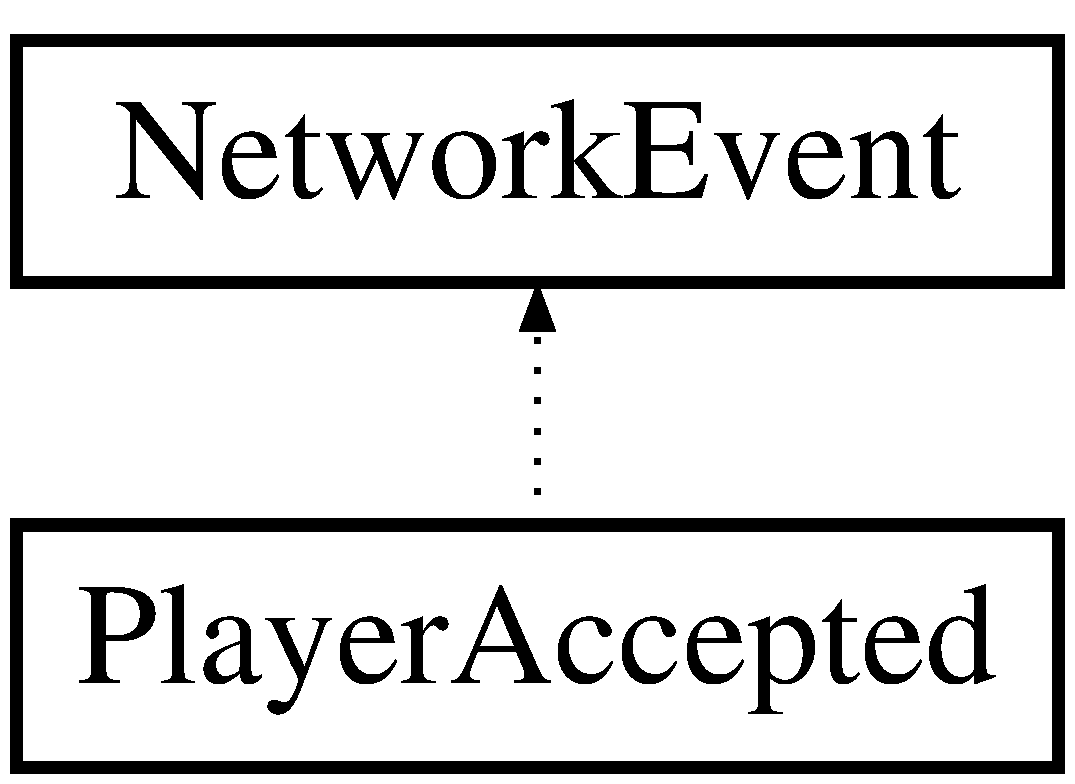
\includegraphics[height=2.000000cm]{class_player_accepted}
\end{center}
\end{figure}
\subsection*{Public Member Functions}
\begin{DoxyCompactItemize}
\item 
\hypertarget{class_player_accepted_a7dfa94ad07e560162a563b74a034e72f}{virtual sf\-::\-Int32 {\bfseries get\-Command} () const }\label{class_player_accepted_a7dfa94ad07e560162a563b74a034e72f}

\end{DoxyCompactItemize}
\subsection*{Public Attributes}
\begin{DoxyCompactItemize}
\item 
\hypertarget{class_player_accepted_a495498cb7e240734eb0e26422357f9c8}{float {\bfseries server\-Time}}\label{class_player_accepted_a495498cb7e240734eb0e26422357f9c8}

\end{DoxyCompactItemize}
\subsection*{Friends}
\begin{DoxyCompactItemize}
\item 
\hypertarget{class_player_accepted_ade60d3614fa9f334f0cf8f98efd67377}{sf\-::\-Packet \& {\bfseries operator$<$$<$} (sf\-::\-Packet \&lhs, const \hyperlink{class_player_accepted}{Player\-Accepted} \&rhs)}\label{class_player_accepted_ade60d3614fa9f334f0cf8f98efd67377}

\item 
\hypertarget{class_player_accepted_ad6f078e6ef68cc88b509f86bd3f1c892}{sf\-::\-Packet \& {\bfseries operator$>$$>$} (sf\-::\-Packet \&lhs, \hyperlink{class_player_accepted}{Player\-Accepted} \&rhs)}\label{class_player_accepted_ad6f078e6ef68cc88b509f86bd3f1c892}

\end{DoxyCompactItemize}
\subsection*{Additional Inherited Members}


\subsection{Detailed Description}
Event that is sent when the player get accepted to the server. 


\begin{DoxyParams}{Parameters}
{\em \textbackslash{}param} & \\
\hline
\end{DoxyParams}
\begin{DoxyReturn}{Returns}
has the server time so that the player can synch with it. 
\end{DoxyReturn}


The documentation for this class was generated from the following file\-:\begin{DoxyCompactItemize}
\item 
include/Network\-Events.\-h\end{DoxyCompactItemize}

\hypertarget{class_player_authorize}{\section{Player\-Authorize Class Reference}
\label{class_player_authorize}\index{Player\-Authorize@{Player\-Authorize}}
}
Inheritance diagram for Player\-Authorize\-:\begin{figure}[H]
\begin{center}
\leavevmode
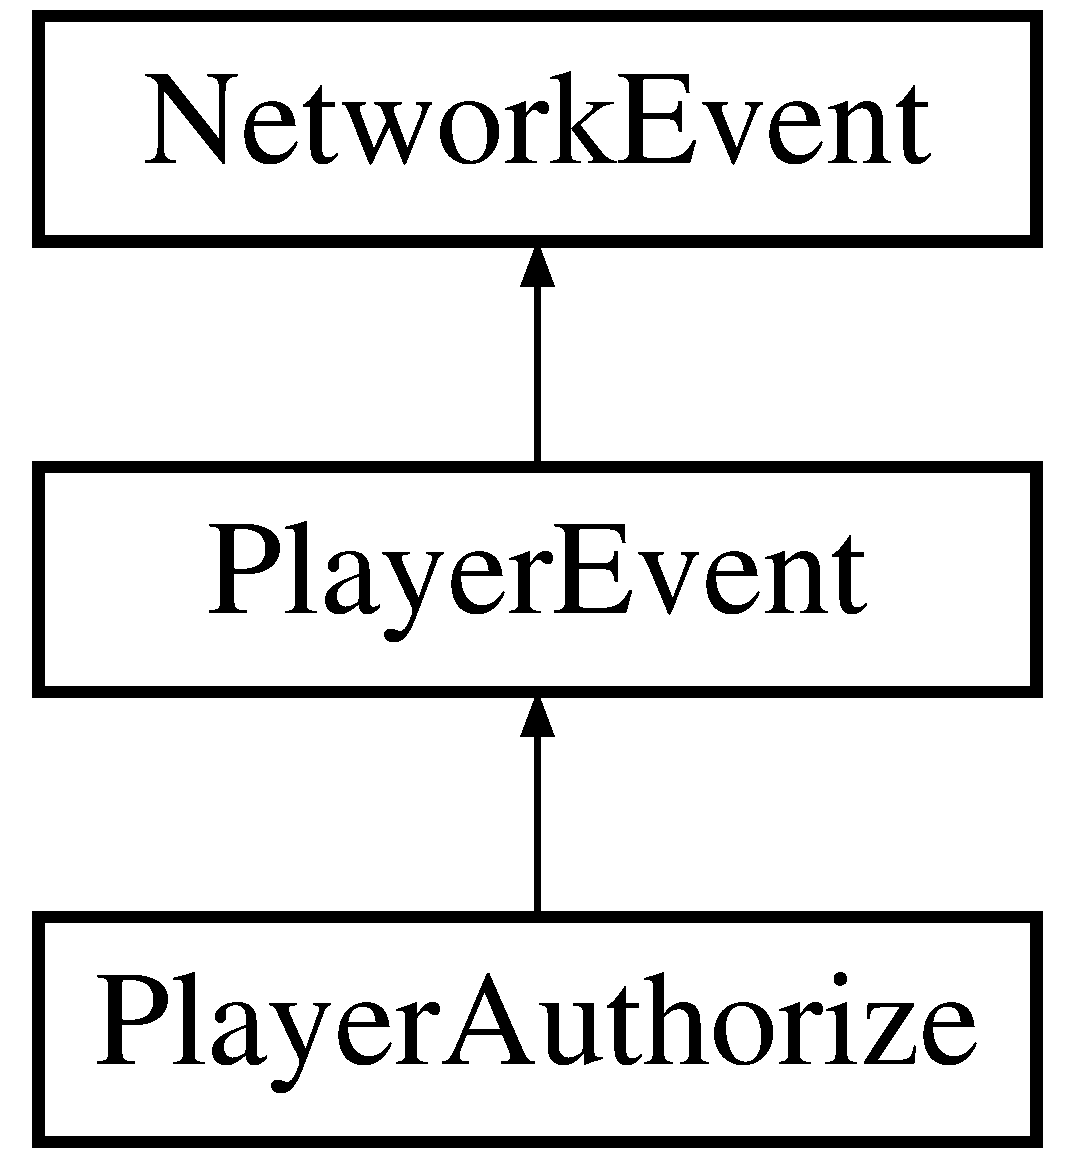
\includegraphics[height=3.000000cm]{class_player_authorize}
\end{center}
\end{figure}
\subsection*{Public Member Functions}
\begin{DoxyCompactItemize}
\item 
\hypertarget{class_player_authorize_ab0f134f275d46bc2d7a04427432468bd}{virtual sf\-::\-Int32 {\bfseries get\-Command} () const }\label{class_player_authorize_ab0f134f275d46bc2d7a04427432468bd}

\end{DoxyCompactItemize}
\subsection*{Public Attributes}
\begin{DoxyCompactItemize}
\item 
\hypertarget{class_player_authorize_acc5cf75a721dff4241d66fccb7aec7b5}{std\-::string {\bfseries password}}\label{class_player_authorize_acc5cf75a721dff4241d66fccb7aec7b5}

\item 
\hypertarget{class_player_authorize_a988ccf8f80f373afce05210d5d98eade}{sf\-::\-Ip\-Address {\bfseries ip}}\label{class_player_authorize_a988ccf8f80f373afce05210d5d98eade}

\item 
\hypertarget{class_player_authorize_ac4b126e0754072f3556afe6f9f050243}{unsigned short {\bfseries port}}\label{class_player_authorize_ac4b126e0754072f3556afe6f9f050243}

\item 
\hypertarget{class_player_authorize_a45af7e978b98ba90b64696f0b9864b37}{bool {\bfseries is\-Registration}}\label{class_player_authorize_a45af7e978b98ba90b64696f0b9864b37}

\end{DoxyCompactItemize}
\subsection*{Friends}
\begin{DoxyCompactItemize}
\item 
\hypertarget{class_player_authorize_a4fee62309b339ef3a35b0b73b70c59bf}{sf\-::\-Packet \& {\bfseries operator$<$$<$} (sf\-::\-Packet \&lhs, const \hyperlink{class_player_authorize}{Player\-Authorize} \&rhs)}\label{class_player_authorize_a4fee62309b339ef3a35b0b73b70c59bf}

\item 
\hypertarget{class_player_authorize_acee74d959a3c4c433ff2ece312ddae0e}{sf\-::\-Packet \& {\bfseries operator$>$$>$} (sf\-::\-Packet \&lhs, \hyperlink{class_player_authorize}{Player\-Authorize} \&rhs)}\label{class_player_authorize_acee74d959a3c4c433ff2ece312ddae0e}

\end{DoxyCompactItemize}
\subsection*{Additional Inherited Members}


The documentation for this class was generated from the following file\-:\begin{DoxyCompactItemize}
\item 
include/Network\-Events.\-h\end{DoxyCompactItemize}

\hypertarget{class_player_connected}{\section{Player\-Connected Class Reference}
\label{class_player_connected}\index{Player\-Connected@{Player\-Connected}}
}


player event connect  




{\ttfamily \#include $<$Network\-Events.\-h$>$}

Inheritance diagram for Player\-Connected\-:\begin{figure}[H]
\begin{center}
\leavevmode
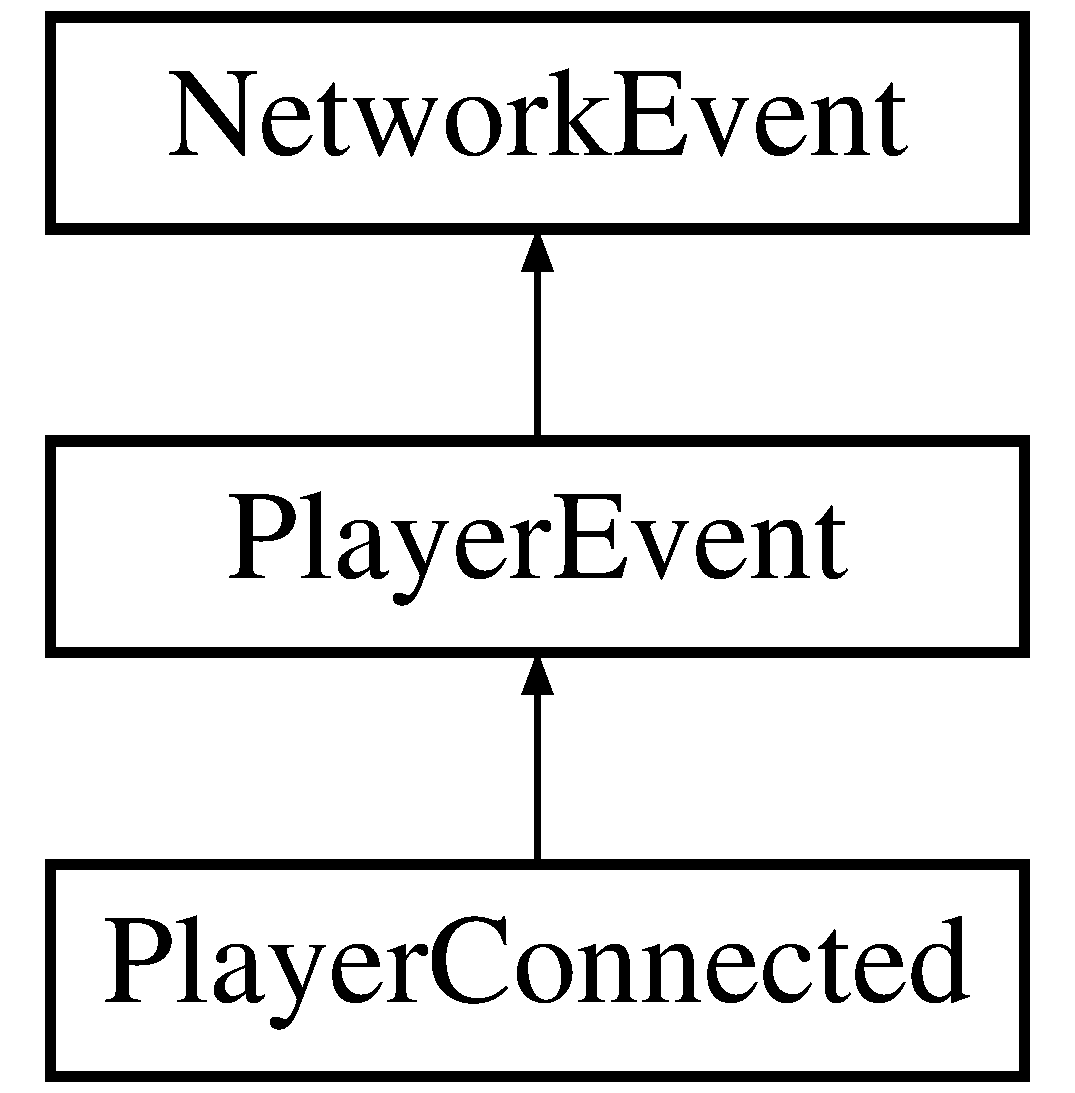
\includegraphics[height=3.000000cm]{class_player_connected}
\end{center}
\end{figure}
\subsection*{Public Member Functions}
\begin{DoxyCompactItemize}
\item 
\hypertarget{class_player_connected_a12e04858807192f0034059bcf2f893d1}{virtual sf\-::\-Int32 {\bfseries get\-Command} () const }\label{class_player_connected_a12e04858807192f0034059bcf2f893d1}

\end{DoxyCompactItemize}
\subsection*{Public Attributes}
\begin{DoxyCompactItemize}
\item 
\hypertarget{class_player_connected_abda0600348cd0b7218fe997bdee16083}{sf\-::\-Color {\bfseries color}}\label{class_player_connected_abda0600348cd0b7218fe997bdee16083}

\end{DoxyCompactItemize}
\subsection*{Friends}
\begin{DoxyCompactItemize}
\item 
\hypertarget{class_player_connected_ad60e9a7caca36f2e5f6bcacac923fae5}{sf\-::\-Packet \& {\bfseries operator$<$$<$} (sf\-::\-Packet \&lhs, const \hyperlink{class_player_connected}{Player\-Connected} \&rhs)}\label{class_player_connected_ad60e9a7caca36f2e5f6bcacac923fae5}

\item 
\hypertarget{class_player_connected_a2d84fc4b49fdf642e87abaa3f7ba09a0}{sf\-::\-Packet \& {\bfseries operator$>$$>$} (sf\-::\-Packet \&lhs, \hyperlink{class_player_connected}{Player\-Connected} \&rhs)}\label{class_player_connected_a2d84fc4b49fdf642e87abaa3f7ba09a0}

\end{DoxyCompactItemize}
\subsection*{Additional Inherited Members}


\subsection{Detailed Description}
player event connect 


\begin{DoxyParams}{Parameters}
{\em \textbackslash{}param} & \\
\hline
\end{DoxyParams}
\begin{DoxyReturn}{Returns}
Send by a connecting player to tell the server that he wants to connect. This message will later contain stuff like password / login vs register 
\end{DoxyReturn}


The documentation for this class was generated from the following file\-:\begin{DoxyCompactItemize}
\item 
include/Network\-Events.\-h\end{DoxyCompactItemize}

\hypertarget{class_player_disconnected}{\section{Player\-Disconnected Class Reference}
\label{class_player_disconnected}\index{Player\-Disconnected@{Player\-Disconnected}}
}


player event disconnect  




{\ttfamily \#include $<$Network\-Events.\-h$>$}

Inheritance diagram for Player\-Disconnected\-:\begin{figure}[H]
\begin{center}
\leavevmode
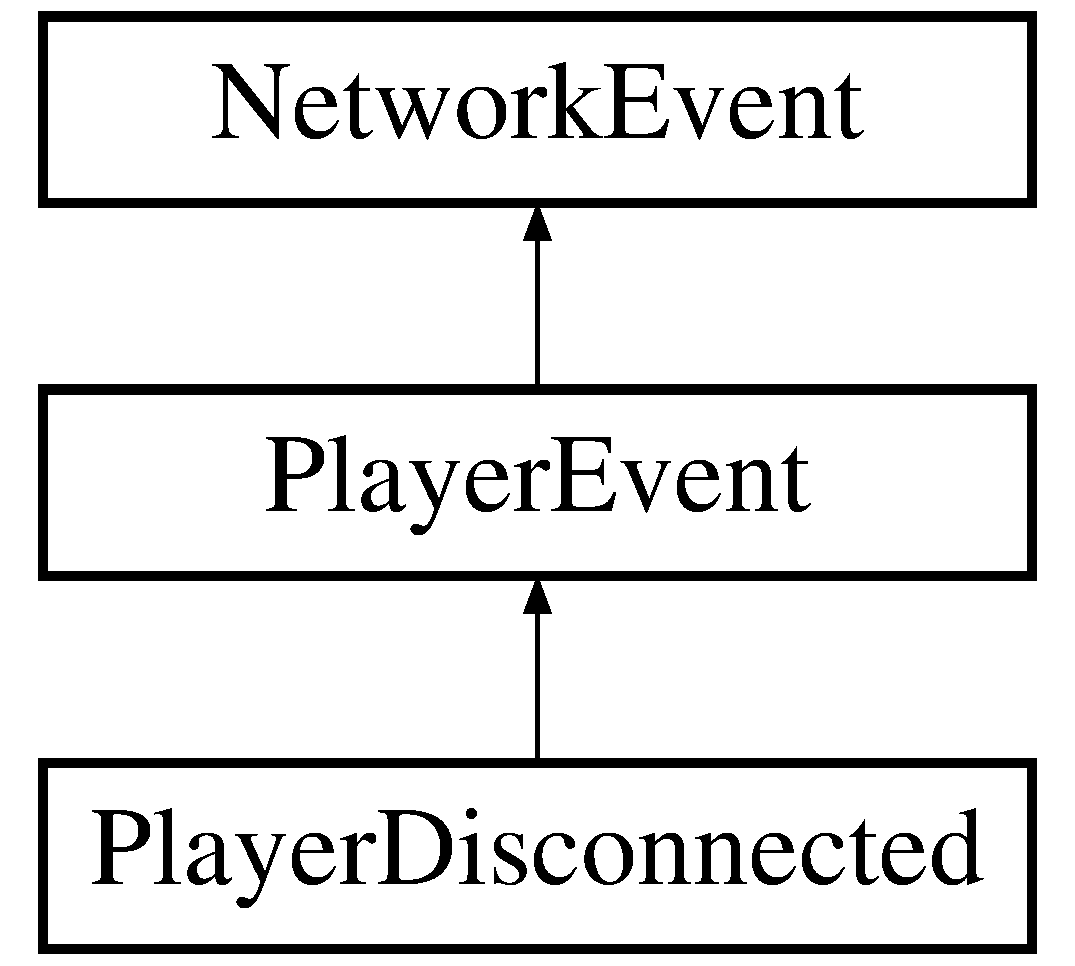
\includegraphics[height=3.000000cm]{class_player_disconnected}
\end{center}
\end{figure}
\subsection*{Public Member Functions}
\begin{DoxyCompactItemize}
\item 
\hypertarget{class_player_disconnected_a4d7130a0e3650f278d9bc260f454426d}{virtual sf\-::\-Int32 {\bfseries get\-Command} () const }\label{class_player_disconnected_a4d7130a0e3650f278d9bc260f454426d}

\end{DoxyCompactItemize}
\subsection*{Friends}
\begin{DoxyCompactItemize}
\item 
\hypertarget{class_player_disconnected_a1f69e293f5bffe2214b5d5fec9e20683}{sf\-::\-Packet \& {\bfseries operator$<$$<$} (sf\-::\-Packet \&lhs, const \hyperlink{class_player_disconnected}{Player\-Disconnected} \&rhs)}\label{class_player_disconnected_a1f69e293f5bffe2214b5d5fec9e20683}

\item 
\hypertarget{class_player_disconnected_a2891f33846a64288367070e78a114e4e}{sf\-::\-Packet \& {\bfseries operator$>$$>$} (sf\-::\-Packet \&lhs, \hyperlink{class_player_disconnected}{Player\-Disconnected} \&rhs)}\label{class_player_disconnected_a2891f33846a64288367070e78a114e4e}

\end{DoxyCompactItemize}
\subsection*{Additional Inherited Members}


\subsection{Detailed Description}
player event disconnect 


\begin{DoxyParams}{Parameters}
{\em \textbackslash{}param} & \\
\hline
\end{DoxyParams}
\begin{DoxyReturn}{Returns}
Ask the server to remove the client from the connected clients 
\end{DoxyReturn}


The documentation for this class was generated from the following file\-:\begin{DoxyCompactItemize}
\item 
include/Network\-Events.\-h\end{DoxyCompactItemize}

\hypertarget{class_player_event}{\section{Player\-Event Class Reference}
\label{class_player_event}\index{Player\-Event@{Player\-Event}}
}


Base Event for player events.  




{\ttfamily \#include $<$Network\-Events.\-h$>$}

Inheritance diagram for Player\-Event\-:\begin{figure}[H]
\begin{center}
\leavevmode
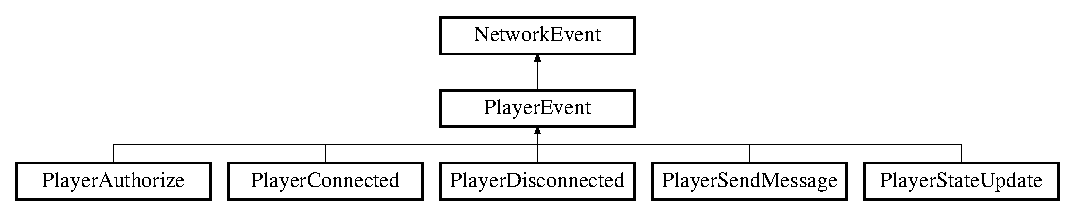
\includegraphics[height=2.452555cm]{class_player_event}
\end{center}
\end{figure}
\subsection*{Public Attributes}
\begin{DoxyCompactItemize}
\item 
\hypertarget{class_player_event_ae3866ad1c76d10e4826bf8599d19a44a}{std\-::string {\bfseries name}}\label{class_player_event_ae3866ad1c76d10e4826bf8599d19a44a}

\end{DoxyCompactItemize}
\subsection*{Additional Inherited Members}


\subsection{Detailed Description}
Base Event for player events. 


\begin{DoxyParams}{Parameters}
{\em \textbackslash{}param} & \\
\hline
\end{DoxyParams}
\begin{DoxyReturn}{Returns}
This will will force all player related events to include a name 
\end{DoxyReturn}


The documentation for this class was generated from the following file\-:\begin{DoxyCompactItemize}
\item 
include/Network\-Events.\-h\end{DoxyCompactItemize}

\hypertarget{class_player_info}{\section{Player\-Info Class Reference}
\label{class_player_info}\index{Player\-Info@{Player\-Info}}
}


Holds info about where players currently are.  




{\ttfamily \#include $<$Network\-Events.\-h$>$}

\subsection*{Public Member Functions}
\begin{DoxyCompactItemize}
\item 
\hypertarget{class_player_info_a7ee6a2ae8e3330c3647d62c10259e111}{\hyperlink{class_player_info}{Player\-Info} \& {\bfseries operator=} (const \hyperlink{class_client}{Client} \&client)}\label{class_player_info_a7ee6a2ae8e3330c3647d62c10259e111}

\end{DoxyCompactItemize}
\subsection*{Public Attributes}
\begin{DoxyCompactItemize}
\item 
\hypertarget{class_player_info_a016f542d46ef9737c0c217643cb48258}{std\-::string {\bfseries name}}\label{class_player_info_a016f542d46ef9737c0c217643cb48258}

\item 
\hypertarget{class_player_info_ae0b4f6e932dabd8643886924b876f2f1}{glm\-::vec2 {\bfseries position}}\label{class_player_info_ae0b4f6e932dabd8643886924b876f2f1}

\end{DoxyCompactItemize}
\subsection*{Friends}
\begin{DoxyCompactItemize}
\item 
\hypertarget{class_player_info_a6e4982eee930a6b74020f304611ef219}{sf\-::\-Packet \& {\bfseries operator$<$$<$} (sf\-::\-Packet \&lhs, const \hyperlink{class_player_info}{Player\-Info} \&player\-Info)}\label{class_player_info_a6e4982eee930a6b74020f304611ef219}

\item 
\hypertarget{class_player_info_a80ed1c47a3f63a380911a85a5ad24ac3}{sf\-::\-Packet \& {\bfseries operator$>$$>$} (sf\-::\-Packet \&lhs, \hyperlink{class_player_info}{Player\-Info} \&player\-Info)}\label{class_player_info_a80ed1c47a3f63a380911a85a5ad24ac3}

\end{DoxyCompactItemize}


\subsection{Detailed Description}
Holds info about where players currently are. 

\begin{DoxyReturn}{Returns}

\end{DoxyReturn}


The documentation for this class was generated from the following files\-:\begin{DoxyCompactItemize}
\item 
include/Network\-Events.\-h\item 
src/Network\-Events.\-cpp\end{DoxyCompactItemize}

\hypertarget{class_player_rejected}{\section{Player\-Rejected Class Reference}
\label{class_player_rejected}\index{Player\-Rejected@{Player\-Rejected}}
}
Inheritance diagram for Player\-Rejected\-:\begin{figure}[H]
\begin{center}
\leavevmode
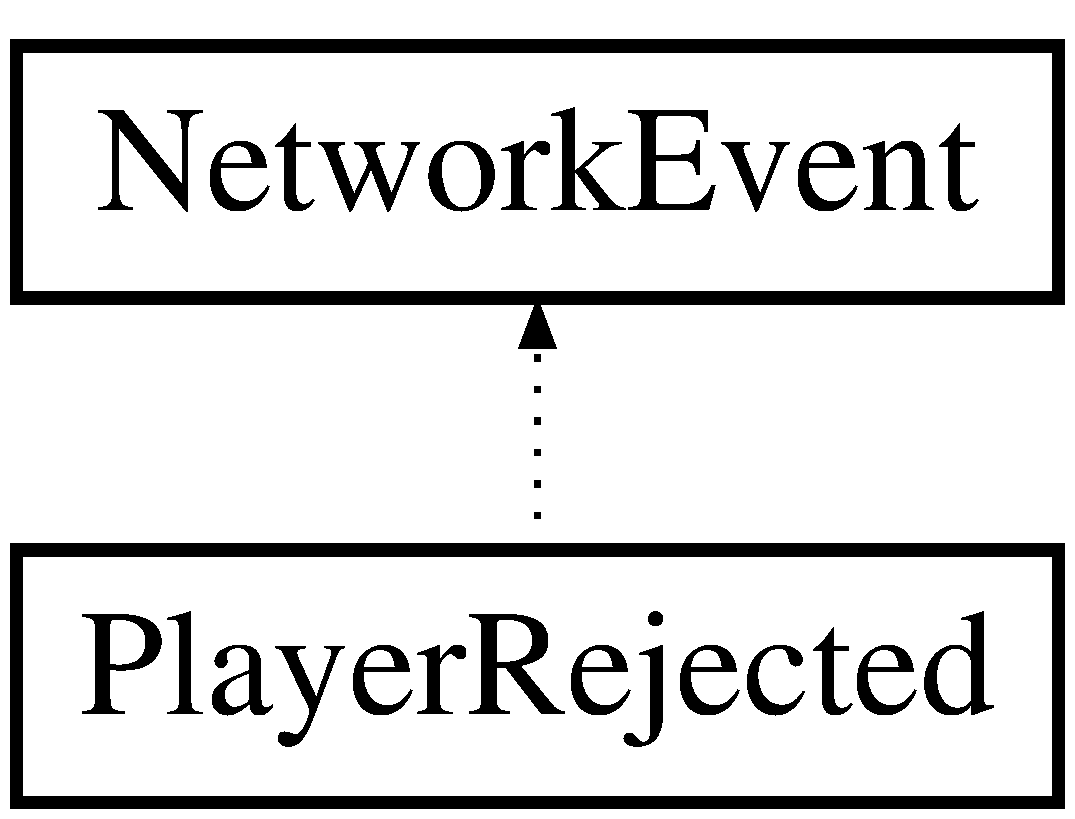
\includegraphics[height=2.000000cm]{class_player_rejected}
\end{center}
\end{figure}
\subsection*{Public Member Functions}
\begin{DoxyCompactItemize}
\item 
\hypertarget{class_player_rejected_adb1c49e808165dc9ab8b7d1455c49188}{virtual sf\-::\-Int32 {\bfseries get\-Command} () const }\label{class_player_rejected_adb1c49e808165dc9ab8b7d1455c49188}

\end{DoxyCompactItemize}
\subsection*{Public Attributes}
\begin{DoxyCompactItemize}
\item 
\hypertarget{class_player_rejected_aa46e86d31cad142d485d63dce947e9a6}{std\-::string {\bfseries reason}}\label{class_player_rejected_aa46e86d31cad142d485d63dce947e9a6}

\end{DoxyCompactItemize}
\subsection*{Friends}
\begin{DoxyCompactItemize}
\item 
\hypertarget{class_player_rejected_a4e7fa10d7a0c4ef94a5dcee8845c6cf8}{sf\-::\-Packet \& {\bfseries operator$<$$<$} (sf\-::\-Packet \&lhs, const \hyperlink{class_player_rejected}{Player\-Rejected} \&rhs)}\label{class_player_rejected_a4e7fa10d7a0c4ef94a5dcee8845c6cf8}

\item 
\hypertarget{class_player_rejected_afb28a903ec29fe9a7ba7bdeea8345140}{sf\-::\-Packet \& {\bfseries operator$>$$>$} (sf\-::\-Packet \&lhs, \hyperlink{class_player_rejected}{Player\-Rejected} \&rhs)}\label{class_player_rejected_afb28a903ec29fe9a7ba7bdeea8345140}

\end{DoxyCompactItemize}
\subsection*{Additional Inherited Members}


The documentation for this class was generated from the following file\-:\begin{DoxyCompactItemize}
\item 
include/Network\-Events.\-h\end{DoxyCompactItemize}

\hypertarget{class_player_send_message}{\section{Player\-Send\-Message Class Reference}
\label{class_player_send_message}\index{Player\-Send\-Message@{Player\-Send\-Message}}
}


player event send message  




{\ttfamily \#include $<$Network\-Events.\-h$>$}

Inheritance diagram for Player\-Send\-Message\-:\begin{figure}[H]
\begin{center}
\leavevmode
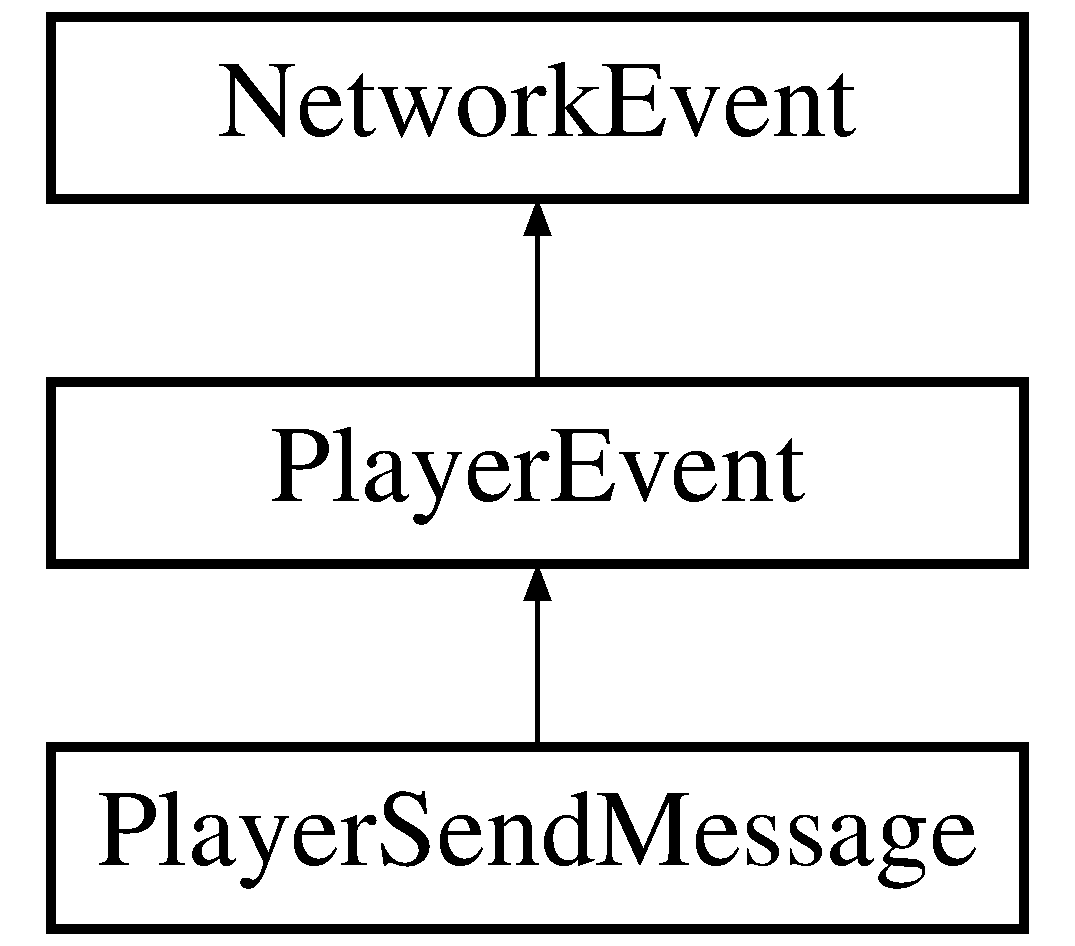
\includegraphics[height=3.000000cm]{class_player_send_message}
\end{center}
\end{figure}
\subsection*{Public Member Functions}
\begin{DoxyCompactItemize}
\item 
\hypertarget{class_player_send_message_a982d585bbc44d7bb2ca0a866654e19fe}{virtual sf\-::\-Int32 {\bfseries get\-Command} () const }\label{class_player_send_message_a982d585bbc44d7bb2ca0a866654e19fe}

\end{DoxyCompactItemize}
\subsection*{Public Attributes}
\begin{DoxyCompactItemize}
\item 
\hypertarget{class_player_send_message_aed484c51804e0df83dd59a162fd62b33}{std\-::string {\bfseries message}}\label{class_player_send_message_aed484c51804e0df83dd59a162fd62b33}

\end{DoxyCompactItemize}
\subsection*{Friends}
\begin{DoxyCompactItemize}
\item 
\hypertarget{class_player_send_message_a6b7d49cde2d46ceabc7d9bd6c9039217}{sf\-::\-Packet \& {\bfseries operator$<$$<$} (sf\-::\-Packet \&lhs, const \hyperlink{class_player_send_message}{Player\-Send\-Message} \&rhs)}\label{class_player_send_message_a6b7d49cde2d46ceabc7d9bd6c9039217}

\item 
\hypertarget{class_player_send_message_ad65ad6dec4004a991901f00db0421d55}{sf\-::\-Packet \& {\bfseries operator$>$$>$} (sf\-::\-Packet \&lhs, \hyperlink{class_player_send_message}{Player\-Send\-Message} \&rhs)}\label{class_player_send_message_ad65ad6dec4004a991901f00db0421d55}

\end{DoxyCompactItemize}
\subsection*{Additional Inherited Members}


\subsection{Detailed Description}
player event send message 


\begin{DoxyParams}{Parameters}
{\em \textbackslash{}param} & \\
\hline
\end{DoxyParams}
\begin{DoxyReturn}{Returns}
Ask the server to broadcast a message to all connected players 
\end{DoxyReturn}


The documentation for this class was generated from the following file\-:\begin{DoxyCompactItemize}
\item 
include/Network\-Events.\-h\end{DoxyCompactItemize}

\hypertarget{class_player_state_update}{\section{Player\-State\-Update Class Reference}
\label{class_player_state_update}\index{Player\-State\-Update@{Player\-State\-Update}}
}


Package containing info about all players connected to the server.  




{\ttfamily \#include $<$Network\-Events.\-h$>$}

Inheritance diagram for Player\-State\-Update\-:\begin{figure}[H]
\begin{center}
\leavevmode
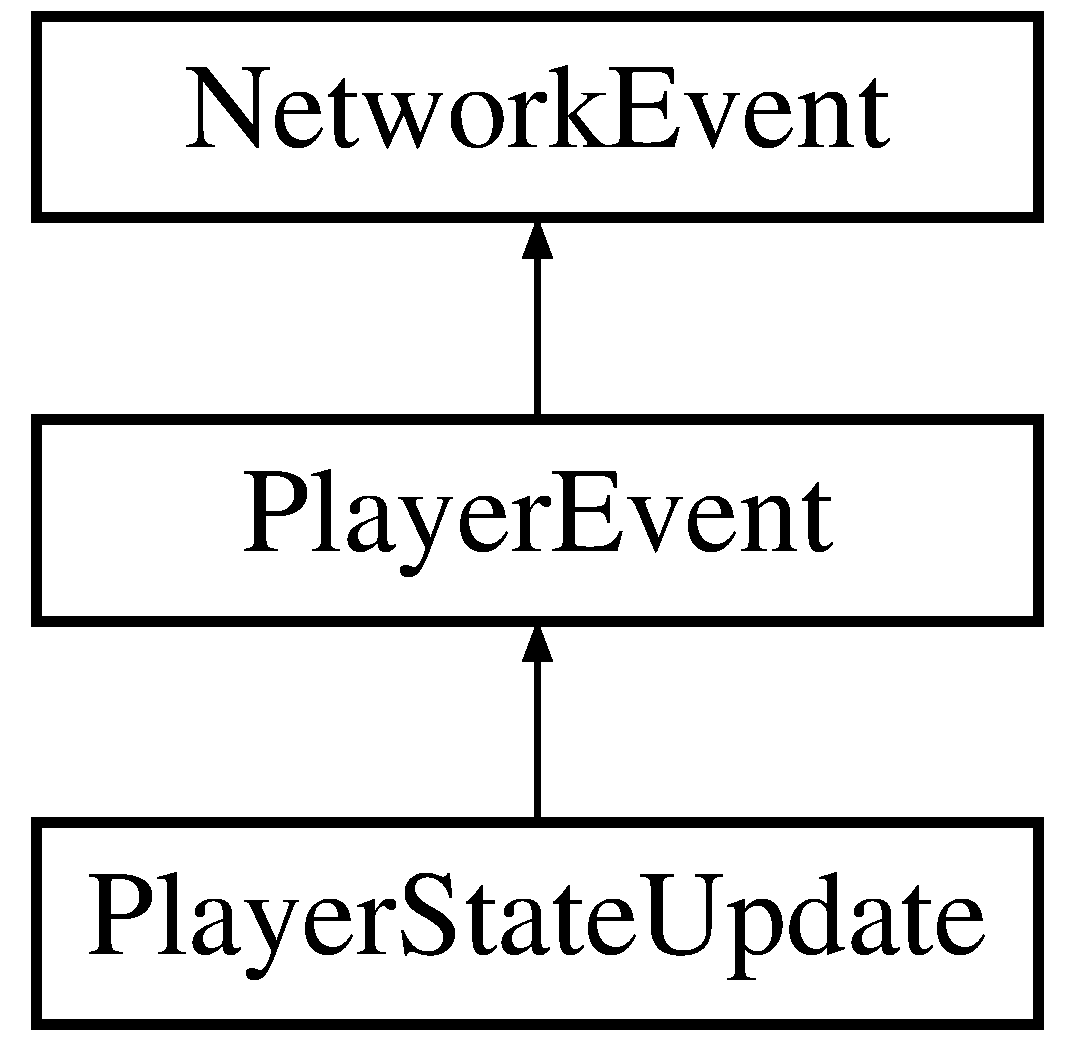
\includegraphics[height=3.000000cm]{class_player_state_update}
\end{center}
\end{figure}
\subsection*{Public Member Functions}
\begin{DoxyCompactItemize}
\item 
\hypertarget{class_player_state_update_abd83649334f18d98f0ead15689f59a57}{virtual sf\-::\-Int32 {\bfseries get\-Command} () const }\label{class_player_state_update_abd83649334f18d98f0ead15689f59a57}

\end{DoxyCompactItemize}
\subsection*{Public Attributes}
\begin{DoxyCompactItemize}
\item 
\hypertarget{class_player_state_update_a4711991bf997f3fe2c5076f2151fe9ba}{\hyperlink{class_key_state}{Key\-State} {\bfseries key\-State}}\label{class_player_state_update_a4711991bf997f3fe2c5076f2151fe9ba}

\item 
\hypertarget{class_player_state_update_a62c4352fcc8469da9b498065d1e024d9}{float {\bfseries receive\-Time}}\label{class_player_state_update_a62c4352fcc8469da9b498065d1e024d9}

\item 
\hypertarget{class_player_state_update_a78f5ddfeaa3e94a0ef7b1d98a0c96084}{glm\-::vec2 {\bfseries position}}\label{class_player_state_update_a78f5ddfeaa3e94a0ef7b1d98a0c96084}

\end{DoxyCompactItemize}
\subsection*{Friends}
\begin{DoxyCompactItemize}
\item 
\hypertarget{class_player_state_update_a276309adde0b77f085d87e4f80537576}{sf\-::\-Packet \& {\bfseries operator$<$$<$} (sf\-::\-Packet \&lhs, const \hyperlink{class_player_state_update}{Player\-State\-Update} \&rhs)}\label{class_player_state_update_a276309adde0b77f085d87e4f80537576}

\item 
\hypertarget{class_player_state_update_a096b592daeee8ee7932d8989074149f9}{sf\-::\-Packet \& {\bfseries operator$>$$>$} (sf\-::\-Packet \&lhs, \hyperlink{class_player_state_update}{Player\-State\-Update} \&rhs)}\label{class_player_state_update_a096b592daeee8ee7932d8989074149f9}

\end{DoxyCompactItemize}
\subsection*{Additional Inherited Members}


\subsection{Detailed Description}
Package containing info about all players connected to the server. 



The documentation for this class was generated from the following file\-:\begin{DoxyCompactItemize}
\item 
include/Network\-Events.\-h\end{DoxyCompactItemize}

\hypertarget{class_player_update_to_client}{\section{Player\-Update\-To\-Client Class Reference}
\label{class_player_update_to_client}\index{Player\-Update\-To\-Client@{Player\-Update\-To\-Client}}
}
Inheritance diagram for Player\-Update\-To\-Client\-:\begin{figure}[H]
\begin{center}
\leavevmode
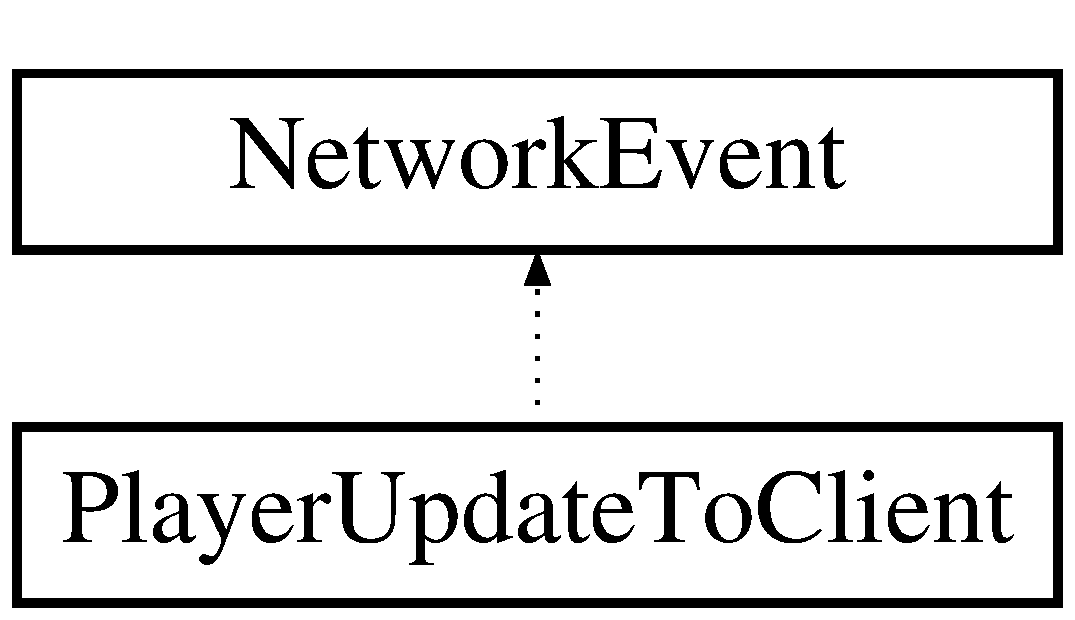
\includegraphics[height=2.000000cm]{class_player_update_to_client}
\end{center}
\end{figure}
\subsection*{Public Member Functions}
\begin{DoxyCompactItemize}
\item 
\hypertarget{class_player_update_to_client_ad712b93f45274f211505baf1280d3e9d}{virtual sf\-::\-Int32 {\bfseries get\-Command} () const }\label{class_player_update_to_client_ad712b93f45274f211505baf1280d3e9d}

\end{DoxyCompactItemize}
\subsection*{Public Attributes}
\begin{DoxyCompactItemize}
\item 
\hypertarget{class_player_update_to_client_a9966a1fa7568a2ecdf9d8f320cb0df94}{float {\bfseries server\-Time}}\label{class_player_update_to_client_a9966a1fa7568a2ecdf9d8f320cb0df94}

\item 
\hypertarget{class_player_update_to_client_a2fd273dcefa40ee10cead19bbf1cfc27}{sf\-::\-Uint32 {\bfseries entry\-Count}}\label{class_player_update_to_client_a2fd273dcefa40ee10cead19bbf1cfc27}

\item 
\hypertarget{class_player_update_to_client_a38b8e97d764d26b4a13f3dea93beec7f}{std\-::vector$<$ \hyperlink{class_player_state_update}{Player\-State\-Update} $>$ {\bfseries players}}\label{class_player_update_to_client_a38b8e97d764d26b4a13f3dea93beec7f}

\end{DoxyCompactItemize}
\subsection*{Friends}
\begin{DoxyCompactItemize}
\item 
\hypertarget{class_player_update_to_client_a7c36f60e30110d0ed1f12279de182ccd}{sf\-::\-Packet \& {\bfseries operator$<$$<$} (sf\-::\-Packet \&lhs, const \hyperlink{class_player_update_to_client}{Player\-Update\-To\-Client} \&rhs)}\label{class_player_update_to_client_a7c36f60e30110d0ed1f12279de182ccd}

\item 
\hypertarget{class_player_update_to_client_a37c118890f7376a2c87e43bbd6e89e4d}{sf\-::\-Packet \& {\bfseries operator$>$$>$} (sf\-::\-Packet \&lhs, \hyperlink{class_player_update_to_client}{Player\-Update\-To\-Client} \&rhs)}\label{class_player_update_to_client_a37c118890f7376a2c87e43bbd6e89e4d}

\end{DoxyCompactItemize}
\subsection*{Additional Inherited Members}


The documentation for this class was generated from the following file\-:\begin{DoxyCompactItemize}
\item 
include/Network\-Events.\-h\end{DoxyCompactItemize}

\hypertarget{structprevious__mode__data}{\section{previous\-\_\-mode\-\_\-data Struct Reference}
\label{structprevious__mode__data}\index{previous\-\_\-mode\-\_\-data@{previous\-\_\-mode\-\_\-data}}
}
\subsection*{Public Attributes}
\begin{DoxyCompactItemize}
\item 
\hypertarget{structprevious__mode__data_a0e739c09db970af70b080b011bd7b313}{int {\bfseries valid}}\label{structprevious__mode__data_a0e739c09db970af70b080b011bd7b313}

\item 
\hypertarget{structprevious__mode__data_affec08bf41351e87a503ea2100f1699a}{int {\bfseries mode}}\label{structprevious__mode__data_affec08bf41351e87a503ea2100f1699a}

\item 
\hypertarget{structprevious__mode__data_af12c8f5a7060d22aec1653274c48412a}{int {\bfseries show\-Header}}\label{structprevious__mode__data_af12c8f5a7060d22aec1653274c48412a}

\item 
\hypertarget{structprevious__mode__data_a5f3ed3d6f0f8fce802648dfa3922783b}{int {\bfseries col\-Width} \mbox{[}100\mbox{]}}\label{structprevious__mode__data_a5f3ed3d6f0f8fce802648dfa3922783b}

\end{DoxyCompactItemize}


The documentation for this struct was generated from the following file\-:\begin{DoxyCompactItemize}
\item 
src/shell.\-c\end{DoxyCompactItemize}

\hypertarget{class_json_1_1_reader}{\section{Json\-:\-:Reader Class Reference}
\label{class_json_1_1_reader}\index{Json\-::\-Reader@{Json\-::\-Reader}}
}


Unserialize a \href{http://www.json.org}{\tt J\-S\-O\-N} document into a \hyperlink{class_json_1_1_value}{Value}.  




{\ttfamily \#include $<$json.\-h$>$}

\subsection*{Public Types}
\begin{DoxyCompactItemize}
\item 
\hypertarget{class_json_1_1_reader_a3eec9118f3e9a672ba8348c3a79d0f45}{typedef char {\bfseries Char}}\label{class_json_1_1_reader_a3eec9118f3e9a672ba8348c3a79d0f45}

\item 
\hypertarget{class_json_1_1_reader_a46795b5b272bf79a7730e406cb96375a}{typedef const Char $\ast$ {\bfseries Location}}\label{class_json_1_1_reader_a46795b5b272bf79a7730e406cb96375a}

\end{DoxyCompactItemize}
\subsection*{Public Member Functions}
\begin{DoxyCompactItemize}
\item 
\hypertarget{class_json_1_1_reader_a0b3c4e24c8393354bab57a6ba3ffc27f}{\hyperlink{class_json_1_1_reader_a0b3c4e24c8393354bab57a6ba3ffc27f}{Reader} ()}\label{class_json_1_1_reader_a0b3c4e24c8393354bab57a6ba3ffc27f}

\begin{DoxyCompactList}\small\item\em Constructs a \hyperlink{class_json_1_1_reader}{Reader} allowing all features for parsing. \end{DoxyCompactList}\item 
\hypertarget{class_json_1_1_reader_a45f17831118337309180313e93ac33f8}{\hyperlink{class_json_1_1_reader_a45f17831118337309180313e93ac33f8}{Reader} (const \hyperlink{class_json_1_1_features}{Features} \&features)}\label{class_json_1_1_reader_a45f17831118337309180313e93ac33f8}

\begin{DoxyCompactList}\small\item\em Constructs a \hyperlink{class_json_1_1_reader}{Reader} allowing the specified feature set for parsing. \end{DoxyCompactList}\item 
bool \hyperlink{class_json_1_1_reader_af1da6c976ad1e96c742804c3853eef94}{parse} (const std\-::string \&document, \hyperlink{class_json_1_1_value}{Value} \&root, bool collect\-Comments=true)
\begin{DoxyCompactList}\small\item\em Read a \hyperlink{class_json_1_1_value}{Value} from a \href{http://www.json.org}{\tt J\-S\-O\-N} document. \end{DoxyCompactList}\item 
bool \hyperlink{class_json_1_1_reader_ac71ef2b64c7c27b062052e692af3fb32}{parse} (const char $\ast$begin\-Doc, const char $\ast$end\-Doc, \hyperlink{class_json_1_1_value}{Value} \&root, bool collect\-Comments=true)
\begin{DoxyCompactList}\small\item\em Read a \hyperlink{class_json_1_1_value}{Value} from a \href{http://www.json.org}{\tt J\-S\-O\-N} document. \end{DoxyCompactList}\item 
bool \hyperlink{class_json_1_1_reader_a8d0347e6b47343e4bc68be7ecdb9c4e9}{parse} (std\-::istream \&is, \hyperlink{class_json_1_1_value}{Value} \&root, bool collect\-Comments=true)
\begin{DoxyCompactList}\small\item\em \hyperlink{struct_parse}{Parse} from input stream. \end{DoxyCompactList}\item 
std\-::string \hyperlink{class_json_1_1_reader_afa4a59e962d23c4d1c38b433fc95eefa}{get\-Formated\-Error\-Messages} () const 
\begin{DoxyCompactList}\small\item\em Returns a user friendly string that list errors in the parsed document. \end{DoxyCompactList}\item 
std\-::string \hyperlink{class_json_1_1_reader_a95ab50aa789132e9dee0fc1475c85acf}{get\-Formatted\-Error\-Messages} () const 
\begin{DoxyCompactList}\small\item\em Returns a user friendly string that list errors in the parsed document. \end{DoxyCompactList}\end{DoxyCompactItemize}


\subsection{Detailed Description}
Unserialize a \href{http://www.json.org}{\tt J\-S\-O\-N} document into a \hyperlink{class_json_1_1_value}{Value}. 



\subsection{Member Function Documentation}
\hypertarget{class_json_1_1_reader_afa4a59e962d23c4d1c38b433fc95eefa}{\index{Json\-::\-Reader@{Json\-::\-Reader}!get\-Formated\-Error\-Messages@{get\-Formated\-Error\-Messages}}
\index{get\-Formated\-Error\-Messages@{get\-Formated\-Error\-Messages}!Json::Reader@{Json\-::\-Reader}}
\subsubsection[{get\-Formated\-Error\-Messages}]{\setlength{\rightskip}{0pt plus 5cm}std\-::string Json\-::\-Reader\-::get\-Formated\-Error\-Messages (
\begin{DoxyParamCaption}
{}
\end{DoxyParamCaption}
) const}}\label{class_json_1_1_reader_afa4a59e962d23c4d1c38b433fc95eefa}


Returns a user friendly string that list errors in the parsed document. 

\begin{DoxyReturn}{Returns}
Formatted error message with the list of errors with their location in the parsed document. An empty string is returned if no error occurred during parsing. 
\end{DoxyReturn}
\begin{DoxyRefDesc}{Deprecated}
\item[\hyperlink{deprecated__deprecated000001}{Deprecated}]Use \hyperlink{class_json_1_1_reader_a95ab50aa789132e9dee0fc1475c85acf}{get\-Formatted\-Error\-Messages()} instead (typo fix). \end{DoxyRefDesc}
\hypertarget{class_json_1_1_reader_a95ab50aa789132e9dee0fc1475c85acf}{\index{Json\-::\-Reader@{Json\-::\-Reader}!get\-Formatted\-Error\-Messages@{get\-Formatted\-Error\-Messages}}
\index{get\-Formatted\-Error\-Messages@{get\-Formatted\-Error\-Messages}!Json::Reader@{Json\-::\-Reader}}
\subsubsection[{get\-Formatted\-Error\-Messages}]{\setlength{\rightskip}{0pt plus 5cm}std\-::string Json\-::\-Reader\-::get\-Formatted\-Error\-Messages (
\begin{DoxyParamCaption}
{}
\end{DoxyParamCaption}
) const}}\label{class_json_1_1_reader_a95ab50aa789132e9dee0fc1475c85acf}


Returns a user friendly string that list errors in the parsed document. 

\begin{DoxyReturn}{Returns}
Formatted error message with the list of errors with their location in the parsed document. An empty string is returned if no error occurred during parsing. 
\end{DoxyReturn}
\hypertarget{class_json_1_1_reader_af1da6c976ad1e96c742804c3853eef94}{\index{Json\-::\-Reader@{Json\-::\-Reader}!parse@{parse}}
\index{parse@{parse}!Json::Reader@{Json\-::\-Reader}}
\subsubsection[{parse}]{\setlength{\rightskip}{0pt plus 5cm}bool Json\-::\-Reader\-::parse (
\begin{DoxyParamCaption}
\item[{const std\-::string \&}]{document, }
\item[{{\bf Value} \&}]{root, }
\item[{bool}]{collect\-Comments = {\ttfamily true}}
\end{DoxyParamCaption}
)}}\label{class_json_1_1_reader_af1da6c976ad1e96c742804c3853eef94}


Read a \hyperlink{class_json_1_1_value}{Value} from a \href{http://www.json.org}{\tt J\-S\-O\-N} document. 


\begin{DoxyParams}{Parameters}
{\em document} & U\-T\-F-\/8 encoded string containing the document to read. \\
\hline
{\em root} & \mbox{[}out\mbox{]} Contains the root value of the document if it was successfully parsed. \\
\hline
{\em collect\-Comments} & {\ttfamily true} to collect comment and allow writing them back during serialization, {\ttfamily false} to discard comments. This parameter is ignored if \hyperlink{class_json_1_1_features_a33afd389719624b6bdb23950b3c346c9}{Features\-::allow\-Comments\-\_\-} is {\ttfamily false}. \\
\hline
\end{DoxyParams}
\begin{DoxyReturn}{Returns}
{\ttfamily true} if the document was successfully parsed, {\ttfamily false} if an error occurred. 
\end{DoxyReturn}
\hypertarget{class_json_1_1_reader_ac71ef2b64c7c27b062052e692af3fb32}{\index{Json\-::\-Reader@{Json\-::\-Reader}!parse@{parse}}
\index{parse@{parse}!Json::Reader@{Json\-::\-Reader}}
\subsubsection[{parse}]{\setlength{\rightskip}{0pt plus 5cm}bool Json\-::\-Reader\-::parse (
\begin{DoxyParamCaption}
\item[{const char $\ast$}]{begin\-Doc, }
\item[{const char $\ast$}]{end\-Doc, }
\item[{{\bf Value} \&}]{root, }
\item[{bool}]{collect\-Comments = {\ttfamily true}}
\end{DoxyParamCaption}
)}}\label{class_json_1_1_reader_ac71ef2b64c7c27b062052e692af3fb32}


Read a \hyperlink{class_json_1_1_value}{Value} from a \href{http://www.json.org}{\tt J\-S\-O\-N} document. 


\begin{DoxyParams}{Parameters}
{\em begin\-Doc} & Pointer on the beginning of the U\-T\-F-\/8 encoded string of the document to read. \\
\hline
{\em end\-Doc} & Pointer on the end of the U\-T\-F-\/8 encoded string of the document to read. \textbackslash{} Must be $>$= begin\-Doc. \\
\hline
{\em root} & \mbox{[}out\mbox{]} Contains the root value of the document if it was successfully parsed. \\
\hline
{\em collect\-Comments} & {\ttfamily true} to collect comment and allow writing them back during serialization, {\ttfamily false} to discard comments. This parameter is ignored if \hyperlink{class_json_1_1_features_a33afd389719624b6bdb23950b3c346c9}{Features\-::allow\-Comments\-\_\-} is {\ttfamily false}. \\
\hline
\end{DoxyParams}
\begin{DoxyReturn}{Returns}
{\ttfamily true} if the document was successfully parsed, {\ttfamily false} if an error occurred. 
\end{DoxyReturn}
\hypertarget{class_json_1_1_reader_a8d0347e6b47343e4bc68be7ecdb9c4e9}{\index{Json\-::\-Reader@{Json\-::\-Reader}!parse@{parse}}
\index{parse@{parse}!Json::Reader@{Json\-::\-Reader}}
\subsubsection[{parse}]{\setlength{\rightskip}{0pt plus 5cm}bool Json\-::\-Reader\-::parse (
\begin{DoxyParamCaption}
\item[{std\-::istream \&}]{is, }
\item[{{\bf Value} \&}]{root, }
\item[{bool}]{collect\-Comments = {\ttfamily true}}
\end{DoxyParamCaption}
)}}\label{class_json_1_1_reader_a8d0347e6b47343e4bc68be7ecdb9c4e9}


\hyperlink{struct_parse}{Parse} from input stream. 

\begin{DoxySeeAlso}{See Also}
\hyperlink{namespace_json_a4d245ef719cc0853e8e78eb5f99c16e5}{Json\-::operator$>$$>$(std\-::istream\&, Json\-::\-Value\&)}. 
\end{DoxySeeAlso}


The documentation for this class was generated from the following files\-:\begin{DoxyCompactItemize}
\item 
include/json/json.\-h\item 
src/jsoncpp.\-cpp\end{DoxyCompactItemize}

\hypertarget{struct_row_set}{\section{Row\-Set Struct Reference}
\label{struct_row_set}\index{Row\-Set@{Row\-Set}}
}
\subsection*{Public Attributes}
\begin{DoxyCompactItemize}
\item 
\hypertarget{struct_row_set_af064f9ec7b1ba820a3d53622bde9d42f}{struct \hyperlink{struct_row_set_chunk}{Row\-Set\-Chunk} $\ast$ {\bfseries p\-Chunk}}\label{struct_row_set_af064f9ec7b1ba820a3d53622bde9d42f}

\item 
\hypertarget{struct_row_set_a7da847a06c2f90025fbd89c57516c6f6}{\hyperlink{structsqlite3}{sqlite3} $\ast$ {\bfseries db}}\label{struct_row_set_a7da847a06c2f90025fbd89c57516c6f6}

\item 
\hypertarget{struct_row_set_a3eccaf69ad7863abae2541a7c0b94e1d}{struct \hyperlink{struct_row_set_entry}{Row\-Set\-Entry} $\ast$ {\bfseries p\-Entry}}\label{struct_row_set_a3eccaf69ad7863abae2541a7c0b94e1d}

\item 
\hypertarget{struct_row_set_a040c4b798e6f20d20aa99a45e93b2079}{struct \hyperlink{struct_row_set_entry}{Row\-Set\-Entry} $\ast$ {\bfseries p\-Last}}\label{struct_row_set_a040c4b798e6f20d20aa99a45e93b2079}

\item 
\hypertarget{struct_row_set_a7c4e95bd08ff77135068bb3987be5ca1}{struct \hyperlink{struct_row_set_entry}{Row\-Set\-Entry} $\ast$ {\bfseries p\-Fresh}}\label{struct_row_set_a7c4e95bd08ff77135068bb3987be5ca1}

\item 
\hypertarget{struct_row_set_abe7ab16fffbe5992f637d6a17c6342ff}{struct \hyperlink{struct_row_set_entry}{Row\-Set\-Entry} $\ast$ {\bfseries p\-Forest}}\label{struct_row_set_abe7ab16fffbe5992f637d6a17c6342ff}

\item 
\hypertarget{struct_row_set_a0ed2a47d6789a70081f3454ef2604e7f}{u16 {\bfseries n\-Fresh}}\label{struct_row_set_a0ed2a47d6789a70081f3454ef2604e7f}

\item 
\hypertarget{struct_row_set_af62438d96429ac10fcbddeb4f6bd9343}{u8 {\bfseries rs\-Flags}}\label{struct_row_set_af62438d96429ac10fcbddeb4f6bd9343}

\item 
\hypertarget{struct_row_set_af33d206290792936cb1ebbb8e03baf64}{u8 {\bfseries i\-Batch}}\label{struct_row_set_af33d206290792936cb1ebbb8e03baf64}

\end{DoxyCompactItemize}


The documentation for this struct was generated from the following file\-:\begin{DoxyCompactItemize}
\item 
src/sqlite3.\-c\end{DoxyCompactItemize}

\hypertarget{struct_row_set_chunk}{\section{Row\-Set\-Chunk Struct Reference}
\label{struct_row_set_chunk}\index{Row\-Set\-Chunk@{Row\-Set\-Chunk}}
}
\subsection*{Public Attributes}
\begin{DoxyCompactItemize}
\item 
\hypertarget{struct_row_set_chunk_ae8f0975c86633ae2bb8b212d3a767554}{struct \hyperlink{struct_row_set_chunk}{Row\-Set\-Chunk} $\ast$ {\bfseries p\-Next\-Chunk}}\label{struct_row_set_chunk_ae8f0975c86633ae2bb8b212d3a767554}

\item 
\hypertarget{struct_row_set_chunk_abde97bbb07c3bf9454e719ff860bdd1f}{struct \hyperlink{struct_row_set_entry}{Row\-Set\-Entry} {\bfseries a\-Entry} \mbox{[}R\-O\-W\-S\-E\-T\-\_\-\-E\-N\-T\-R\-Y\-\_\-\-P\-E\-R\-\_\-\-C\-H\-U\-N\-K\mbox{]}}\label{struct_row_set_chunk_abde97bbb07c3bf9454e719ff860bdd1f}

\end{DoxyCompactItemize}


The documentation for this struct was generated from the following file\-:\begin{DoxyCompactItemize}
\item 
src/sqlite3.\-c\end{DoxyCompactItemize}

\hypertarget{struct_row_set_entry}{\section{Row\-Set\-Entry Struct Reference}
\label{struct_row_set_entry}\index{Row\-Set\-Entry@{Row\-Set\-Entry}}
}
\subsection*{Public Attributes}
\begin{DoxyCompactItemize}
\item 
\hypertarget{struct_row_set_entry_ac72670935246f1bff5e4d96703574071}{i64 {\bfseries v}}\label{struct_row_set_entry_ac72670935246f1bff5e4d96703574071}

\item 
\hypertarget{struct_row_set_entry_ac39c09525dd24f42af522587d1bc5026}{struct \hyperlink{struct_row_set_entry}{Row\-Set\-Entry} $\ast$ {\bfseries p\-Right}}\label{struct_row_set_entry_ac39c09525dd24f42af522587d1bc5026}

\item 
\hypertarget{struct_row_set_entry_a59365203c30ce782ae38e534c90db14b}{struct \hyperlink{struct_row_set_entry}{Row\-Set\-Entry} $\ast$ {\bfseries p\-Left}}\label{struct_row_set_entry_a59365203c30ce782ae38e534c90db14b}

\end{DoxyCompactItemize}


The documentation for this struct was generated from the following file\-:\begin{DoxyCompactItemize}
\item 
src/sqlite3.\-c\end{DoxyCompactItemize}

\hypertarget{struct_savepoint}{\section{Savepoint Struct Reference}
\label{struct_savepoint}\index{Savepoint@{Savepoint}}
}
\subsection*{Public Attributes}
\begin{DoxyCompactItemize}
\item 
\hypertarget{struct_savepoint_a0ba08ea77fcfd93099288375e2e9b1ec}{char $\ast$ {\bfseries z\-Name}}\label{struct_savepoint_a0ba08ea77fcfd93099288375e2e9b1ec}

\item 
\hypertarget{struct_savepoint_ae00dd8f725701d9e31da2edbb0b27435}{i64 {\bfseries n\-Deferred\-Cons}}\label{struct_savepoint_ae00dd8f725701d9e31da2edbb0b27435}

\item 
\hypertarget{struct_savepoint_a8d785c3c0eeb6f0c62ea5391892c78cb}{\hyperlink{struct_savepoint}{Savepoint} $\ast$ {\bfseries p\-Next}}\label{struct_savepoint_a8d785c3c0eeb6f0c62ea5391892c78cb}

\end{DoxyCompactItemize}


The documentation for this struct was generated from the following file\-:\begin{DoxyCompactItemize}
\item 
src/sqlite3.\-c\end{DoxyCompactItemize}

\hypertarget{class_scene}{\section{Scene Class Reference}
\label{class_scene}\index{Scene@{Scene}}
}
\subsection*{Public Member Functions}
\begin{DoxyCompactItemize}
\item 
\hypertarget{class_scene_a80794b261fa465fb93ce273a0ce2caca}{{\bfseries Scene} (sf\-::\-Render\-Window \&window, \hyperlink{class_game}{Game} \&game)}\label{class_scene_a80794b261fa465fb93ce273a0ce2caca}

\item 
\hypertarget{class_scene_aa24c7e636c10e4e42650c1374b90bb80}{void {\bfseries update} ()}\label{class_scene_aa24c7e636c10e4e42650c1374b90bb80}

\item 
\hypertarget{class_scene_a6c04883087016b9448e5599d2e34422c}{void {\bfseries cleanup} ()}\label{class_scene_a6c04883087016b9448e5599d2e34422c}

\item 
\hypertarget{class_scene_ac0e3d2c98ba6063a086467fb2c19142f}{void {\bfseries draw} ()}\label{class_scene_ac0e3d2c98ba6063a086467fb2c19142f}

\item 
\hypertarget{class_scene_a1b7c88ec2c1a88943d5b79b37f5abe49}{void {\bfseries create\-Character} ()}\label{class_scene_a1b7c88ec2c1a88943d5b79b37f5abe49}

\item 
\hypertarget{class_scene_ade38b7ea256a5531b31305303e9a655a}{\hyperlink{class_networked_character}{Networked\-Character} $\ast$ {\bfseries create\-Networked\-Character} (std\-::string name, const sf\-::\-Color \&color)}\label{class_scene_ade38b7ea256a5531b31305303e9a655a}

\item 
\hypertarget{class_scene_aae77284da4e2622e7a47bf3fe29a2662}{void {\bfseries remove\-Networked\-Character} (std\-::string name)}\label{class_scene_aae77284da4e2622e7a47bf3fe29a2662}

\item 
\hypertarget{class_scene_a85ec2e74504cc6e7f6ad42832652b976}{void {\bfseries add\-To\-Scene} (\hyperlink{class_game_object}{Game\-Object} \&go)}\label{class_scene_a85ec2e74504cc6e7f6ad42832652b976}

\item 
\hypertarget{class_scene_ae854b91fa936f14feb3c60604abfc921}{void {\bfseries load\-Level} (const std\-::string \&name)}\label{class_scene_ae854b91fa936f14feb3c60604abfc921}

\item 
\hypertarget{class_scene_a17010fc67e4338e62813a94e6808cb06}{const \hyperlink{class_level}{Level} $\ast$ {\bfseries get\-Level} () const }\label{class_scene_a17010fc67e4338e62813a94e6808cb06}

\item 
\hypertarget{class_scene_a07fdb7e156c7efb227c6f413ddfa77f0}{void {\bfseries create\-Target} (unsigned int target\-Id, const glm\-::vec2 \&pos)}\label{class_scene_a07fdb7e156c7efb227c6f413ddfa77f0}

\item 
\hypertarget{class_scene_a660b97de1dcd68ff53a61dc38b034153}{void {\bfseries remove\-Target} (unsigned int target\-Id)}\label{class_scene_a660b97de1dcd68ff53a61dc38b034153}

\end{DoxyCompactItemize}


The documentation for this class was generated from the following files\-:\begin{DoxyCompactItemize}
\item 
include/Scene.\-hpp\item 
src/Scene.\-cpp\end{DoxyCompactItemize}

\hypertarget{struct_schema}{\section{Schema Struct Reference}
\label{struct_schema}\index{Schema@{Schema}}
}
\subsection*{Public Attributes}
\begin{DoxyCompactItemize}
\item 
\hypertarget{struct_schema_a3eef54a64f4f962d64577646bd34a47c}{int {\bfseries schema\-\_\-cookie}}\label{struct_schema_a3eef54a64f4f962d64577646bd34a47c}

\item 
\hypertarget{struct_schema_a879b1597656c7cbcbb98cdb88e876874}{int {\bfseries i\-Generation}}\label{struct_schema_a879b1597656c7cbcbb98cdb88e876874}

\item 
\hypertarget{struct_schema_af841eadc93b289944b95f72b784bfaae}{\hyperlink{struct_hash}{Hash} {\bfseries tbl\-Hash}}\label{struct_schema_af841eadc93b289944b95f72b784bfaae}

\item 
\hypertarget{struct_schema_ac0dd242f486d17ddadca1e47af76c6c5}{\hyperlink{struct_hash}{Hash} {\bfseries idx\-Hash}}\label{struct_schema_ac0dd242f486d17ddadca1e47af76c6c5}

\item 
\hypertarget{struct_schema_ab521f4545d200329d8e1a46bbb67e7c5}{\hyperlink{struct_hash}{Hash} {\bfseries trig\-Hash}}\label{struct_schema_ab521f4545d200329d8e1a46bbb67e7c5}

\item 
\hypertarget{struct_schema_ad51ed96351701cfe8d9e871722827c11}{\hyperlink{struct_hash}{Hash} {\bfseries fkey\-Hash}}\label{struct_schema_ad51ed96351701cfe8d9e871722827c11}

\item 
\hypertarget{struct_schema_ad580e4e662724bee95571d297f94da37}{\hyperlink{struct_table}{Table} $\ast$ {\bfseries p\-Seq\-Tab}}\label{struct_schema_ad580e4e662724bee95571d297f94da37}

\item 
\hypertarget{struct_schema_ab9f0371436e41b3080772995407a4cca}{u8 {\bfseries file\-\_\-format}}\label{struct_schema_ab9f0371436e41b3080772995407a4cca}

\item 
\hypertarget{struct_schema_a1338d09fe9cbb5a8162929202cb73cae}{u8 {\bfseries enc}}\label{struct_schema_a1338d09fe9cbb5a8162929202cb73cae}

\item 
\hypertarget{struct_schema_a14838766a0a438e590a27f300beff459}{u16 {\bfseries flags}}\label{struct_schema_a14838766a0a438e590a27f300beff459}

\item 
\hypertarget{struct_schema_a0a66691be95a30c099ca4840da7110dd}{int {\bfseries cache\-\_\-size}}\label{struct_schema_a0a66691be95a30c099ca4840da7110dd}

\end{DoxyCompactItemize}


The documentation for this struct was generated from the following file\-:\begin{DoxyCompactItemize}
\item 
src/sqlite3.\-c\end{DoxyCompactItemize}

\hypertarget{struct_f_key_1_1s_col_map}{\section{F\-Key\-:\-:s\-Col\-Map Struct Reference}
\label{struct_f_key_1_1s_col_map}\index{F\-Key\-::s\-Col\-Map@{F\-Key\-::s\-Col\-Map}}
}
\subsection*{Public Attributes}
\begin{DoxyCompactItemize}
\item 
\hypertarget{struct_f_key_1_1s_col_map_a2b0ed19d4924a93d1f3f14f891b176ed}{int {\bfseries i\-From}}\label{struct_f_key_1_1s_col_map_a2b0ed19d4924a93d1f3f14f891b176ed}

\item 
\hypertarget{struct_f_key_1_1s_col_map_a4cdef475be73cc460873051a2c2c2937}{char $\ast$ {\bfseries z\-Col}}\label{struct_f_key_1_1s_col_map_a4cdef475be73cc460873051a2c2c2937}

\end{DoxyCompactItemize}


The documentation for this struct was generated from the following file\-:\begin{DoxyCompactItemize}
\item 
src/sqlite3.\-c\end{DoxyCompactItemize}

\hypertarget{class_score_change}{\section{Score\-Change Class Reference}
\label{class_score_change}\index{Score\-Change@{Score\-Change}}
}
Inheritance diagram for Score\-Change\-:\begin{figure}[H]
\begin{center}
\leavevmode
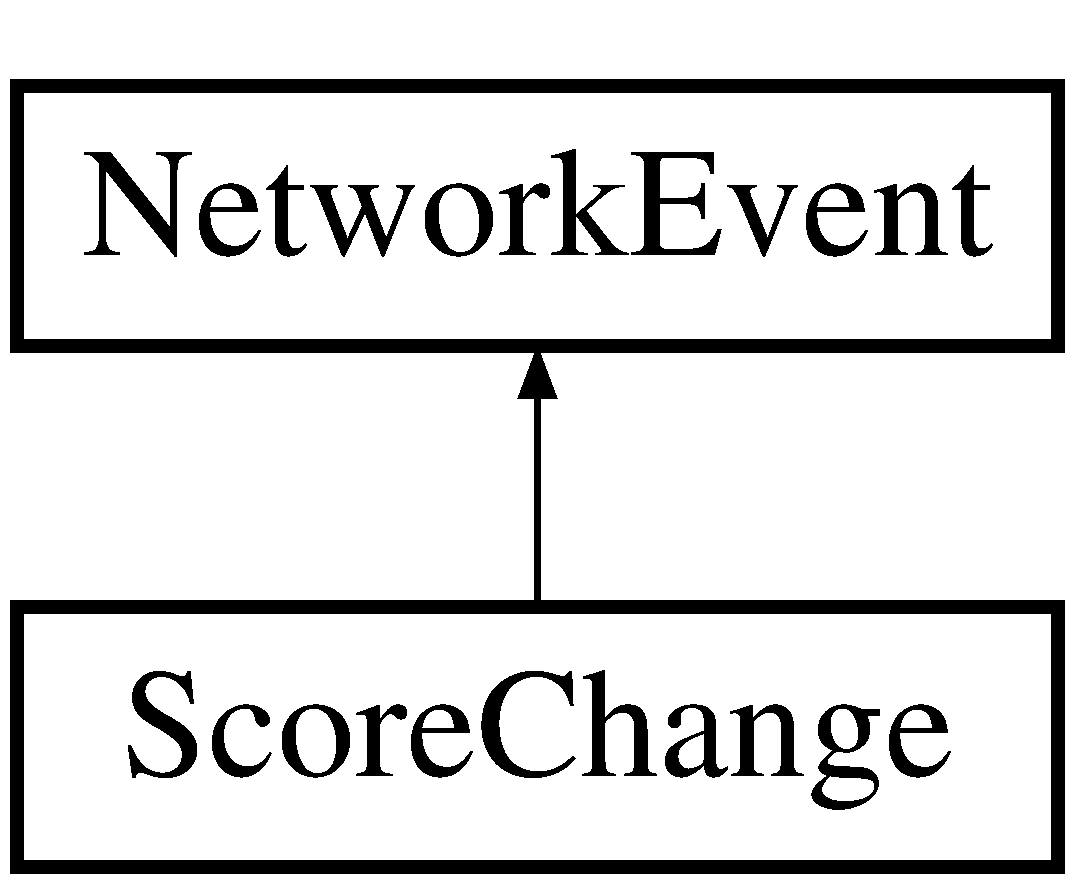
\includegraphics[height=2.000000cm]{class_score_change}
\end{center}
\end{figure}
\subsection*{Public Member Functions}
\begin{DoxyCompactItemize}
\item 
\hypertarget{class_score_change_a4e5b48b2651c1ac8139ddb5a63ab2c7e}{virtual sf\-::\-Int32 {\bfseries get\-Command} () const }\label{class_score_change_a4e5b48b2651c1ac8139ddb5a63ab2c7e}

\end{DoxyCompactItemize}
\subsection*{Public Attributes}
\begin{DoxyCompactItemize}
\item 
\hypertarget{class_score_change_a68080c0e280f46d57a0dbb14854a9580}{unsigned int {\bfseries entry\-Count}}\label{class_score_change_a68080c0e280f46d57a0dbb14854a9580}

\item 
\hypertarget{class_score_change_a48a51fac5ced15ec32daaf2e778d42f1}{std\-::vector$<$ \hyperlink{struct_score_object}{Score\-Object} $>$ {\bfseries score\-Objects}}\label{class_score_change_a48a51fac5ced15ec32daaf2e778d42f1}

\end{DoxyCompactItemize}
\subsection*{Friends}
\begin{DoxyCompactItemize}
\item 
\hypertarget{class_score_change_a11ea360d235b8e4c32070d5817693663}{sf\-::\-Packet \& {\bfseries operator$<$$<$} (sf\-::\-Packet \&packet, const \hyperlink{class_score_change}{Score\-Change} \&tar)}\label{class_score_change_a11ea360d235b8e4c32070d5817693663}

\item 
\hypertarget{class_score_change_a7764eb6d9ec7a6ff87fdf38f211440db}{sf\-::\-Packet \& {\bfseries operator$>$$>$} (sf\-::\-Packet \&packet, \hyperlink{class_score_change}{Score\-Change} \&tar)}\label{class_score_change_a7764eb6d9ec7a6ff87fdf38f211440db}

\end{DoxyCompactItemize}
\subsection*{Additional Inherited Members}


The documentation for this class was generated from the following file\-:\begin{DoxyCompactItemize}
\item 
include/Network\-Events.\-h\end{DoxyCompactItemize}

\hypertarget{struct_score_object}{\section{Score\-Object Struct Reference}
\label{struct_score_object}\index{Score\-Object@{Score\-Object}}
}
\subsection*{Public Attributes}
\begin{DoxyCompactItemize}
\item 
\hypertarget{struct_score_object_ab978f157e91ca14ed929cd4a0cabc205}{std\-::string {\bfseries name}}\label{struct_score_object_ab978f157e91ca14ed929cd4a0cabc205}

\item 
\hypertarget{struct_score_object_a2fcc4391a8eb6ba7d0abc3e5eb511a97}{int {\bfseries score}}\label{struct_score_object_a2fcc4391a8eb6ba7d0abc3e5eb511a97}

\end{DoxyCompactItemize}
\subsection*{Friends}
\begin{DoxyCompactItemize}
\item 
\hypertarget{struct_score_object_a4242d42272a6f241b88cbfeddab12fa4}{sf\-::\-Packet \& {\bfseries operator$<$$<$} (sf\-::\-Packet \&packet, const \hyperlink{struct_score_object}{Score\-Object} \&score\-Object)}\label{struct_score_object_a4242d42272a6f241b88cbfeddab12fa4}

\item 
\hypertarget{struct_score_object_a4dd140f98a350a014bdd36e1a345d0ee}{sf\-::\-Packet \& {\bfseries operator$>$$>$} (sf\-::\-Packet \&packet, \hyperlink{struct_score_object}{Score\-Object} \&score\-Object)}\label{struct_score_object_a4dd140f98a350a014bdd36e1a345d0ee}

\end{DoxyCompactItemize}


The documentation for this struct was generated from the following file\-:\begin{DoxyCompactItemize}
\item 
include/Network\-Events.\-h\end{DoxyCompactItemize}

\hypertarget{struct_scratch_freeslot}{\section{Scratch\-Freeslot Struct Reference}
\label{struct_scratch_freeslot}\index{Scratch\-Freeslot@{Scratch\-Freeslot}}
}
\subsection*{Public Attributes}
\begin{DoxyCompactItemize}
\item 
\hypertarget{struct_scratch_freeslot_aca5c55a56a2a63a5be0756707a04bee8}{struct \hyperlink{struct_scratch_freeslot}{Scratch\-Freeslot} $\ast$ {\bfseries p\-Next}}\label{struct_scratch_freeslot_aca5c55a56a2a63a5be0756707a04bee8}

\end{DoxyCompactItemize}


The documentation for this struct was generated from the following file\-:\begin{DoxyCompactItemize}
\item 
src/sqlite3.\-c\end{DoxyCompactItemize}

\hypertarget{struct_select}{\section{Select Struct Reference}
\label{struct_select}\index{Select@{Select}}
}
\subsection*{Public Attributes}
\begin{DoxyCompactItemize}
\item 
\hypertarget{struct_select_acf92c5d6b0e0e6a3263a77696baaadc8}{\hyperlink{struct_expr_list}{Expr\-List} $\ast$ {\bfseries p\-E\-List}}\label{struct_select_acf92c5d6b0e0e6a3263a77696baaadc8}

\item 
\hypertarget{struct_select_a84506d61248313b5e10f7891cb7482be}{u8 {\bfseries op}}\label{struct_select_a84506d61248313b5e10f7891cb7482be}

\item 
\hypertarget{struct_select_a1c445561ea66d48573c8d8751108c743}{u16 {\bfseries sel\-Flags}}\label{struct_select_a1c445561ea66d48573c8d8751108c743}

\item 
\hypertarget{struct_select_abf68908bf029af42a32c60a2558a8b1e}{int {\bfseries i\-Limit}}\label{struct_select_abf68908bf029af42a32c60a2558a8b1e}

\item 
\hypertarget{struct_select_ac12bebd00ed988df3ad1efb8e6c63fe4}{int {\bfseries i\-Offset}}\label{struct_select_ac12bebd00ed988df3ad1efb8e6c63fe4}

\item 
\hypertarget{struct_select_a5cad3b59bf1803be552d002e74bdfd47}{int {\bfseries addr\-Open\-Ephm} \mbox{[}3\mbox{]}}\label{struct_select_a5cad3b59bf1803be552d002e74bdfd47}

\item 
\hypertarget{struct_select_a177125317478139f9ce834e4f7a93c52}{double {\bfseries n\-Select\-Row}}\label{struct_select_a177125317478139f9ce834e4f7a93c52}

\item 
\hypertarget{struct_select_a4e3b9b176a8e1b4af988405ff1f090db}{\hyperlink{struct_src_list}{Src\-List} $\ast$ {\bfseries p\-Src}}\label{struct_select_a4e3b9b176a8e1b4af988405ff1f090db}

\item 
\hypertarget{struct_select_a0562c1e19acde263a04af015611d8ce8}{\hyperlink{struct_expr}{Expr} $\ast$ {\bfseries p\-Where}}\label{struct_select_a0562c1e19acde263a04af015611d8ce8}

\item 
\hypertarget{struct_select_a5b625c7495468ae56ca2f214a76231a0}{\hyperlink{struct_expr_list}{Expr\-List} $\ast$ {\bfseries p\-Group\-By}}\label{struct_select_a5b625c7495468ae56ca2f214a76231a0}

\item 
\hypertarget{struct_select_ad09e0b115e6e1599e3075b87dfa6e66e}{\hyperlink{struct_expr}{Expr} $\ast$ {\bfseries p\-Having}}\label{struct_select_ad09e0b115e6e1599e3075b87dfa6e66e}

\item 
\hypertarget{struct_select_a73c474cd4a9a9b9aa4e3187d8bf2d886}{\hyperlink{struct_expr_list}{Expr\-List} $\ast$ {\bfseries p\-Order\-By}}\label{struct_select_a73c474cd4a9a9b9aa4e3187d8bf2d886}

\item 
\hypertarget{struct_select_a51d1a253b0aba5a54b11b3bf3896d056}{\hyperlink{struct_select}{Select} $\ast$ {\bfseries p\-Prior}}\label{struct_select_a51d1a253b0aba5a54b11b3bf3896d056}

\item 
\hypertarget{struct_select_a96aa0caf60390b8f5e88589639205c40}{\hyperlink{struct_select}{Select} $\ast$ {\bfseries p\-Next}}\label{struct_select_a96aa0caf60390b8f5e88589639205c40}

\item 
\hypertarget{struct_select_a6ee045fa4305f1d68be5bdc22555e624}{\hyperlink{struct_select}{Select} $\ast$ {\bfseries p\-Rightmost}}\label{struct_select_a6ee045fa4305f1d68be5bdc22555e624}

\item 
\hypertarget{struct_select_a11d3b48d04d58be818cdefb10aa061a0}{\hyperlink{struct_expr}{Expr} $\ast$ {\bfseries p\-Limit}}\label{struct_select_a11d3b48d04d58be818cdefb10aa061a0}

\item 
\hypertarget{struct_select_aeaf016a10203b911000354122562fb46}{\hyperlink{struct_expr}{Expr} $\ast$ {\bfseries p\-Offset}}\label{struct_select_aeaf016a10203b911000354122562fb46}

\end{DoxyCompactItemize}


The documentation for this struct was generated from the following file\-:\begin{DoxyCompactItemize}
\item 
src/sqlite3.\-c\end{DoxyCompactItemize}

\hypertarget{struct_select_dest}{\section{Select\-Dest Struct Reference}
\label{struct_select_dest}\index{Select\-Dest@{Select\-Dest}}
}
\subsection*{Public Attributes}
\begin{DoxyCompactItemize}
\item 
\hypertarget{struct_select_dest_a779c1809acadd15898db0b20e31cc23f}{u8 {\bfseries e\-Dest}}\label{struct_select_dest_a779c1809acadd15898db0b20e31cc23f}

\item 
\hypertarget{struct_select_dest_a7c58e0aef1d9e1eff03a8d765e7e2395}{char {\bfseries aff\-Sdst}}\label{struct_select_dest_a7c58e0aef1d9e1eff03a8d765e7e2395}

\item 
\hypertarget{struct_select_dest_ad30d63b2b7216a533a5ea476412664aa}{int {\bfseries i\-S\-D\-Parm}}\label{struct_select_dest_ad30d63b2b7216a533a5ea476412664aa}

\item 
\hypertarget{struct_select_dest_adbc1c5f38b8c95da1d05e8c25dee400f}{int {\bfseries i\-Sdst}}\label{struct_select_dest_adbc1c5f38b8c95da1d05e8c25dee400f}

\item 
\hypertarget{struct_select_dest_aa4e7438446ef26231f7426edfda13e19}{int {\bfseries n\-Sdst}}\label{struct_select_dest_aa4e7438446ef26231f7426edfda13e19}

\end{DoxyCompactItemize}


The documentation for this struct was generated from the following file\-:\begin{DoxyCompactItemize}
\item 
src/sqlite3.\-c\end{DoxyCompactItemize}

\hypertarget{class_server}{\section{Server Class Reference}
\label{class_server}\index{Server@{Server}}
}
\subsection*{Public Member Functions}
\begin{DoxyCompactItemize}
\item 
\hyperlink{class_server_ad5ec9462b520e59f7ea831e157ee5e59}{Server} ()
\item 
\hypertarget{class_server_a1b3625b83969e5718b04d13836703372}{void {\bfseries build} ()}\label{class_server_a1b3625b83969e5718b04d13836703372}

\item 
\hypertarget{class_server_abb27d30b40a94326e3fd629d3b30b7d5}{void {\bfseries run} ()}\label{class_server_abb27d30b40a94326e3fd629d3b30b7d5}

\end{DoxyCompactItemize}
\subsection*{Friends}
\begin{DoxyCompactItemize}
\item 
\hypertarget{class_server_a2ba4344f0e28b7c576e84b7c397fa458}{class {\bfseries Server\-Command\-Handler}}\label{class_server_a2ba4344f0e28b7c576e84b7c397fa458}

\end{DoxyCompactItemize}


\subsection{Constructor \& Destructor Documentation}
\hypertarget{class_server_ad5ec9462b520e59f7ea831e157ee5e59}{\index{Server@{Server}!Server@{Server}}
\index{Server@{Server}!Server@{Server}}
\subsubsection[{Server}]{\setlength{\rightskip}{0pt plus 5cm}Server\-::\-Server (
\begin{DoxyParamCaption}
{}
\end{DoxyParamCaption}
)}}\label{class_server_ad5ec9462b520e59f7ea831e157ee5e59}
setting up the socketselector 

The documentation for this class was generated from the following files\-:\begin{DoxyCompactItemize}
\item 
include/Server.\-hpp\item 
src/Server.\-cpp\end{DoxyCompactItemize}

\hypertarget{class_server_command_handler}{\section{Server\-Command\-Handler Class Reference}
\label{class_server_command_handler}\index{Server\-Command\-Handler@{Server\-Command\-Handler}}
}
Inheritance diagram for Server\-Command\-Handler\-:\begin{figure}[H]
\begin{center}
\leavevmode
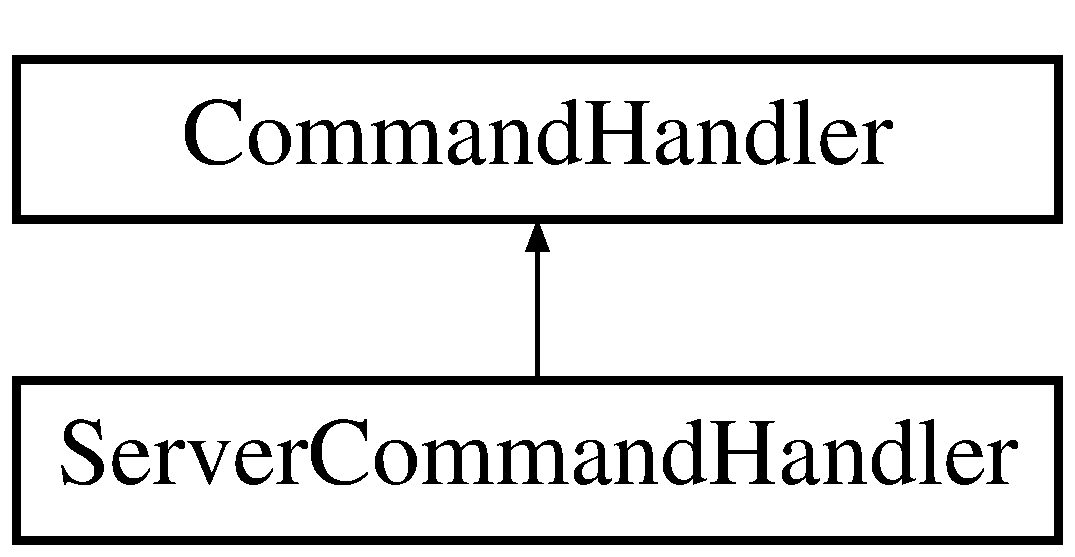
\includegraphics[height=2.000000cm]{class_server_command_handler}
\end{center}
\end{figure}
\subsection*{Public Member Functions}
\begin{DoxyCompactItemize}
\item 
\hypertarget{class_server_command_handler_a9ca785453aa82ddc41ae8ed4c84c8aba}{{\bfseries Server\-Command\-Handler} (\hyperlink{class_server}{Server} \&server)}\label{class_server_command_handler_a9ca785453aa82ddc41ae8ed4c84c8aba}

\end{DoxyCompactItemize}
\subsection*{Protected Member Functions}
\begin{DoxyCompactItemize}
\item 
\hypertarget{class_server_command_handler_a20d91d940ecf08b92b7be38955cd70d1}{virtual void {\bfseries player\-\_\-authorize} (const \hyperlink{class_player_authorize}{Player\-Authorize} \&pe, const sf\-::\-Ip\-Address \&from\-Ip, unsigned short from\-Port)}\label{class_server_command_handler_a20d91d940ecf08b92b7be38955cd70d1}

\item 
\hypertarget{class_server_command_handler_a976eb94c615e3bbb29f0f0312b4ee908}{virtual void {\bfseries player\-\_\-disconnected} (const \hyperlink{class_player_disconnected}{Player\-Disconnected} \&pe)}\label{class_server_command_handler_a976eb94c615e3bbb29f0f0312b4ee908}

\item 
\hypertarget{class_server_command_handler_a99972523ad0a0b7ea677c4ccd99dc48b}{virtual void {\bfseries player\-\_\-send\-\_\-message} (const \hyperlink{class_player_send_message}{Player\-Send\-Message} \&pe)}\label{class_server_command_handler_a99972523ad0a0b7ea677c4ccd99dc48b}

\item 
\hypertarget{class_server_command_handler_aeddc33b88773e622c95c70193724e239}{virtual void {\bfseries server\-\_\-entry\-\_\-accept} (const \hyperlink{class_server_entry_accept}{Server\-Entry\-Accept} \&pe)}\label{class_server_command_handler_aeddc33b88773e622c95c70193724e239}

\item 
\hypertarget{class_server_command_handler_a6f688191f3dc1da888a7f405440ce3a0}{virtual void {\bfseries server\-\_\-entry\-\_\-reject} (const \hyperlink{class_server_entry_reject}{Server\-Entry\-Reject} \&pe)}\label{class_server_command_handler_a6f688191f3dc1da888a7f405440ce3a0}

\item 
\hypertarget{class_server_command_handler_a8ebb5957fd6d83f63d6034805577fcf2}{virtual void {\bfseries player\-\_\-update\-\_\-to\-\_\-server} (const \hyperlink{class_player_state_update}{Player\-State\-Update} \&pe)}\label{class_server_command_handler_a8ebb5957fd6d83f63d6034805577fcf2}

\end{DoxyCompactItemize}


The documentation for this class was generated from the following files\-:\begin{DoxyCompactItemize}
\item 
include/Server\-Command\-Handler.\-hpp\item 
src/Server\-Command\-Handler.\-cpp\end{DoxyCompactItemize}

\hypertarget{class_server_entry}{\section{Server\-Entry Class Reference}
\label{class_server_entry}\index{Server\-Entry@{Server\-Entry}}
}
\subsection*{Public Attributes}
\begin{DoxyCompactItemize}
\item 
\hypertarget{class_server_entry_a2f86249f9ad7b83600b7820f35955ac3}{std\-::string {\bfseries name}}\label{class_server_entry_a2f86249f9ad7b83600b7820f35955ac3}

\item 
\hypertarget{class_server_entry_ace090ceebcb355b23239797ad881b6b9}{sf\-::\-Ip\-Address {\bfseries ip}}\label{class_server_entry_ace090ceebcb355b23239797ad881b6b9}

\end{DoxyCompactItemize}
\subsection*{Friends}
\begin{DoxyCompactItemize}
\item 
\hypertarget{class_server_entry_abbdb757ca7b36097cbfee856d9b0d9fa}{sf\-::\-Packet \& {\bfseries operator$<$$<$} (sf\-::\-Packet \&packet, const \hyperlink{class_server_entry}{Server\-Entry} \&entry)}\label{class_server_entry_abbdb757ca7b36097cbfee856d9b0d9fa}

\item 
\hypertarget{class_server_entry_a24cfd6a036c4bab77e58bcc375b664d1}{sf\-::\-Packet \& {\bfseries operator$>$$>$} (sf\-::\-Packet \&packet, \hyperlink{class_server_entry}{Server\-Entry} \&entry)}\label{class_server_entry_a24cfd6a036c4bab77e58bcc375b664d1}

\end{DoxyCompactItemize}


The documentation for this class was generated from the following file\-:\begin{DoxyCompactItemize}
\item 
include/Network\-Events.\-h\end{DoxyCompactItemize}

\hypertarget{class_server_entry_accept}{\section{Server\-Entry\-Accept Class Reference}
\label{class_server_entry_accept}\index{Server\-Entry\-Accept@{Server\-Entry\-Accept}}
}
Inheritance diagram for Server\-Entry\-Accept\-:\begin{figure}[H]
\begin{center}
\leavevmode
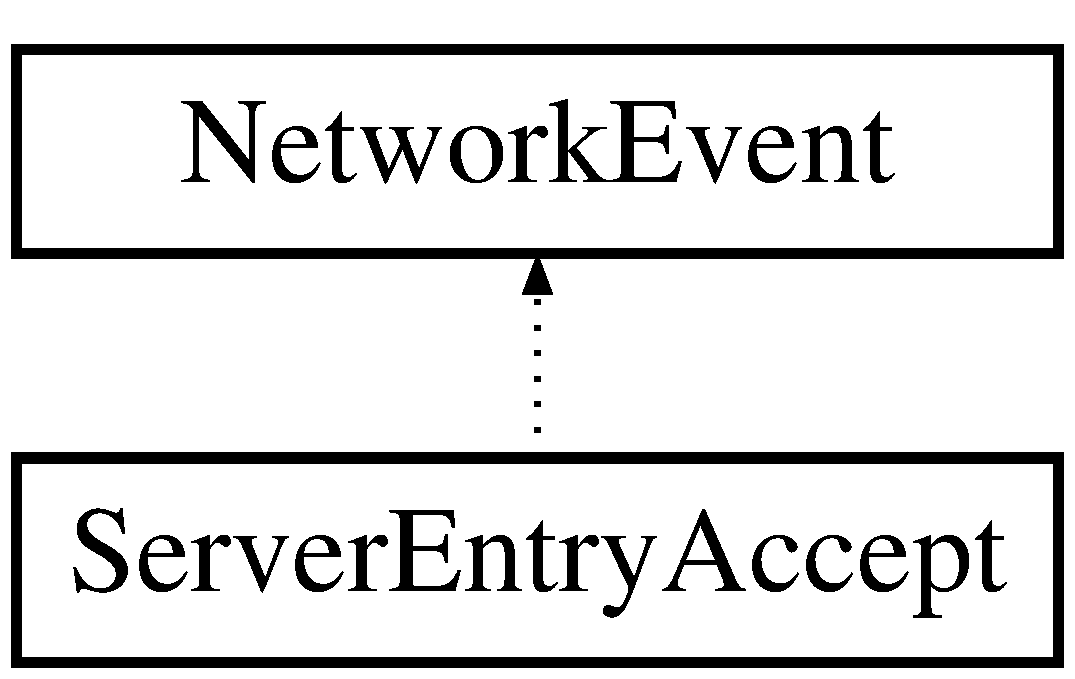
\includegraphics[height=2.000000cm]{class_server_entry_accept}
\end{center}
\end{figure}
\subsection*{Public Member Functions}
\begin{DoxyCompactItemize}
\item 
\hypertarget{class_server_entry_accept_a0fe534df0130c212dbe8ce0e7d8e874a}{virtual sf\-::\-Int32 {\bfseries get\-Command} () const }\label{class_server_entry_accept_a0fe534df0130c212dbe8ce0e7d8e874a}

\end{DoxyCompactItemize}
\subsection*{Friends}
\begin{DoxyCompactItemize}
\item 
\hypertarget{class_server_entry_accept_aa31f51c0b4c88a51b59bff9d010e6a37}{sf\-::\-Packet \& {\bfseries operator$<$$<$} (sf\-::\-Packet \&lhs, const \hyperlink{class_server_entry_accept}{Server\-Entry\-Accept} \&rhs)}\label{class_server_entry_accept_aa31f51c0b4c88a51b59bff9d010e6a37}

\item 
\hypertarget{class_server_entry_accept_a5e4695e9a3e3dec0f606529a96b8d73a}{sf\-::\-Packet \& {\bfseries operator$>$$>$} (sf\-::\-Packet \&lhs, \hyperlink{class_server_entry_accept}{Server\-Entry\-Accept} \&rhs)}\label{class_server_entry_accept_a5e4695e9a3e3dec0f606529a96b8d73a}

\end{DoxyCompactItemize}
\subsection*{Additional Inherited Members}


The documentation for this class was generated from the following file\-:\begin{DoxyCompactItemize}
\item 
include/Network\-Events.\-h\end{DoxyCompactItemize}

\hypertarget{class_server_entry_add}{\section{Server\-Entry\-Add Class Reference}
\label{class_server_entry_add}\index{Server\-Entry\-Add@{Server\-Entry\-Add}}
}


Update that is send from client to server.  




{\ttfamily \#include $<$Network\-Events.\-h$>$}

Inheritance diagram for Server\-Entry\-Add\-:\begin{figure}[H]
\begin{center}
\leavevmode
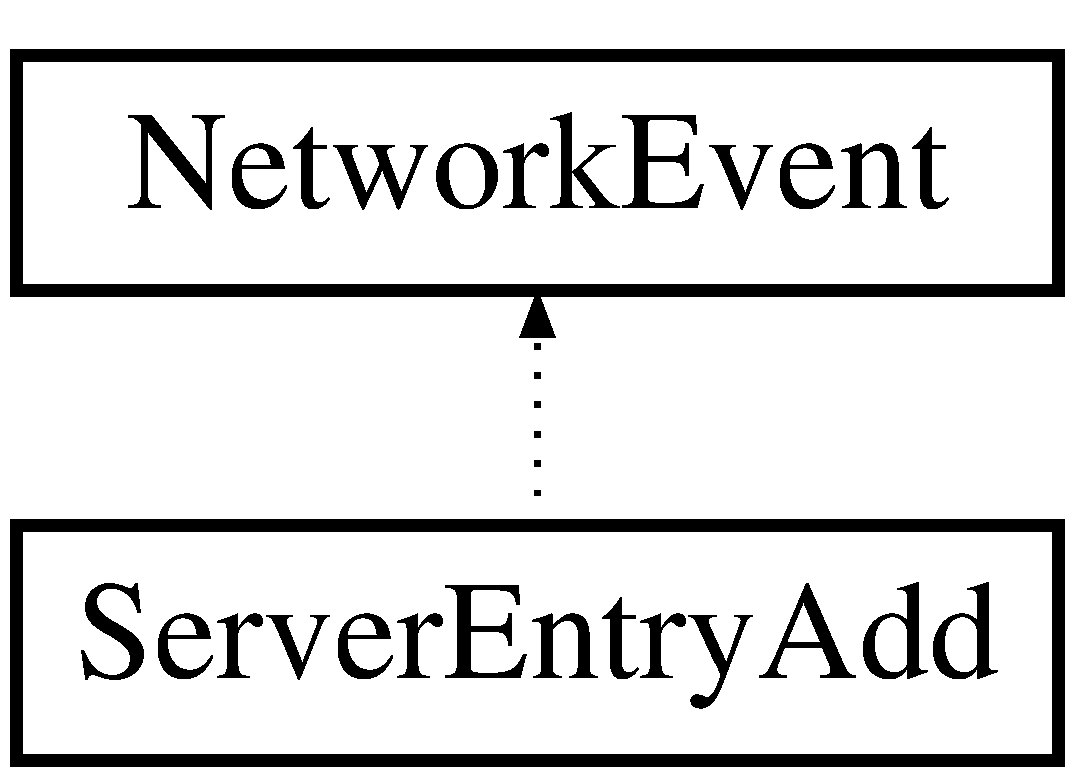
\includegraphics[height=2.000000cm]{class_server_entry_add}
\end{center}
\end{figure}
\subsection*{Public Member Functions}
\begin{DoxyCompactItemize}
\item 
\hypertarget{class_server_entry_add_a90f0f983cafdd6f4cbde987aaa9eaab8}{virtual sf\-::\-Int32 {\bfseries get\-Command} () const }\label{class_server_entry_add_a90f0f983cafdd6f4cbde987aaa9eaab8}

\end{DoxyCompactItemize}
\subsection*{Public Attributes}
\begin{DoxyCompactItemize}
\item 
\hypertarget{class_server_entry_add_aeb277ba2fcd76c69f67b36e32d270fa9}{std\-::string {\bfseries name}}\label{class_server_entry_add_aeb277ba2fcd76c69f67b36e32d270fa9}

\item 
\hypertarget{class_server_entry_add_a9d868e1b9ee3075061be55fd9195568d}{sf\-::\-Ip\-Address {\bfseries ip}}\label{class_server_entry_add_a9d868e1b9ee3075061be55fd9195568d}

\end{DoxyCompactItemize}
\subsection*{Friends}
\begin{DoxyCompactItemize}
\item 
\hypertarget{class_server_entry_add_ad7f9e52ca2a1e66099a0a8e7bf14bb67}{sf\-::\-Packet \& {\bfseries operator$<$$<$} (sf\-::\-Packet \&lhs, const \hyperlink{class_server_entry_add}{Server\-Entry\-Add} \&rhs)}\label{class_server_entry_add_ad7f9e52ca2a1e66099a0a8e7bf14bb67}

\item 
\hypertarget{class_server_entry_add_ab30669e1b81d46a6c3013b8276591a9a}{sf\-::\-Packet \& {\bfseries operator$>$$>$} (sf\-::\-Packet \&lhs, \hyperlink{class_server_entry_add}{Server\-Entry\-Add} \&rhs)}\label{class_server_entry_add_ab30669e1b81d46a6c3013b8276591a9a}

\end{DoxyCompactItemize}
\subsection*{Additional Inherited Members}


\subsection{Detailed Description}
Update that is send from client to server. 


\begin{DoxyParams}{Parameters}
{\em \textbackslash{}param} & \\
\hline
\end{DoxyParams}
\begin{DoxyReturn}{Returns}
Contains the state of the keys 
\end{DoxyReturn}


The documentation for this class was generated from the following file\-:\begin{DoxyCompactItemize}
\item 
include/Network\-Events.\-h\end{DoxyCompactItemize}

\hypertarget{class_server_entry_get}{\section{Server\-Entry\-Get Class Reference}
\label{class_server_entry_get}\index{Server\-Entry\-Get@{Server\-Entry\-Get}}
}
Inheritance diagram for Server\-Entry\-Get\-:\begin{figure}[H]
\begin{center}
\leavevmode
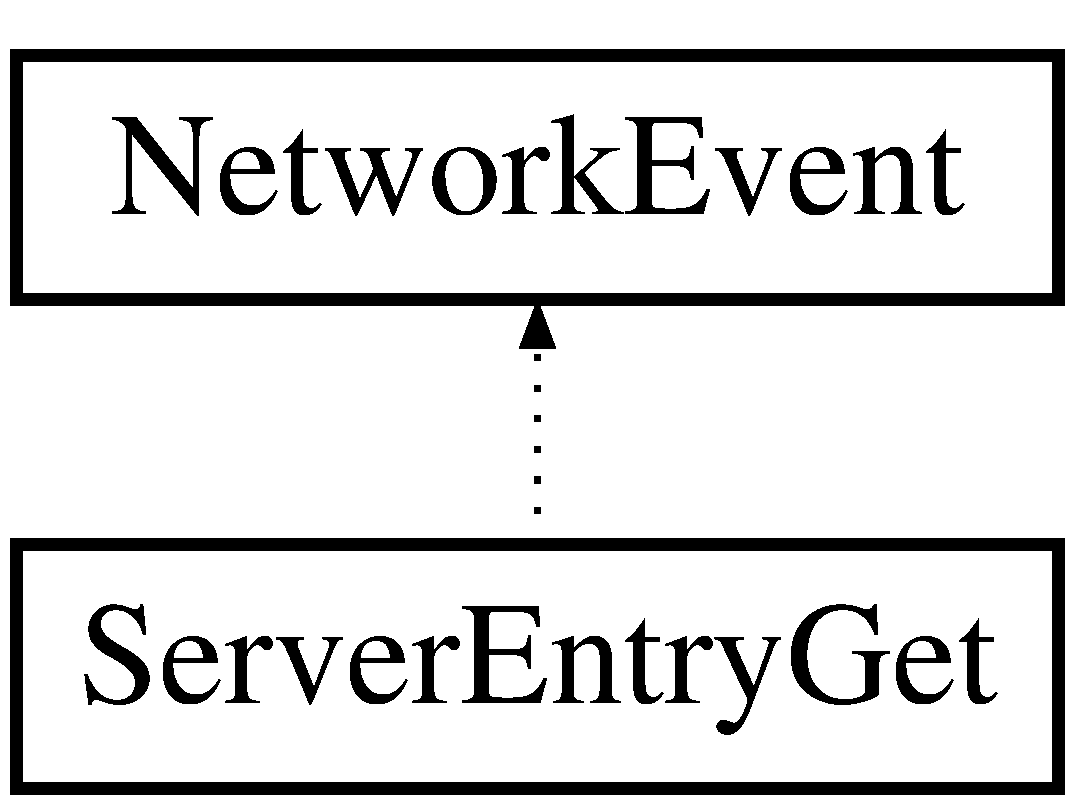
\includegraphics[height=2.000000cm]{class_server_entry_get}
\end{center}
\end{figure}
\subsection*{Public Member Functions}
\begin{DoxyCompactItemize}
\item 
\hypertarget{class_server_entry_get_a8ac2bfd76dde2b9a7a0536cc9b11c64a}{virtual sf\-::\-Int32 {\bfseries get\-Command} () const }\label{class_server_entry_get_a8ac2bfd76dde2b9a7a0536cc9b11c64a}

\end{DoxyCompactItemize}
\subsection*{Friends}
\begin{DoxyCompactItemize}
\item 
\hypertarget{class_server_entry_get_af357ae32ae1296c4c36175512cced91b}{sf\-::\-Packet \& {\bfseries operator$<$$<$} (sf\-::\-Packet \&lhs, const \hyperlink{class_server_entry_get}{Server\-Entry\-Get} \&rhs)}\label{class_server_entry_get_af357ae32ae1296c4c36175512cced91b}

\item 
\hypertarget{class_server_entry_get_abff6a0041fd25a336820678606e0c98c}{sf\-::\-Packet \& {\bfseries operator$>$$>$} (sf\-::\-Packet \&lhs, \hyperlink{class_server_entry_get}{Server\-Entry\-Get} \&rhs)}\label{class_server_entry_get_abff6a0041fd25a336820678606e0c98c}

\end{DoxyCompactItemize}
\subsection*{Additional Inherited Members}


The documentation for this class was generated from the following file\-:\begin{DoxyCompactItemize}
\item 
include/Network\-Events.\-h\end{DoxyCompactItemize}

\hypertarget{class_server_entry_list}{\section{Server\-Entry\-List Class Reference}
\label{class_server_entry_list}\index{Server\-Entry\-List@{Server\-Entry\-List}}
}
Inheritance diagram for Server\-Entry\-List\-:\begin{figure}[H]
\begin{center}
\leavevmode
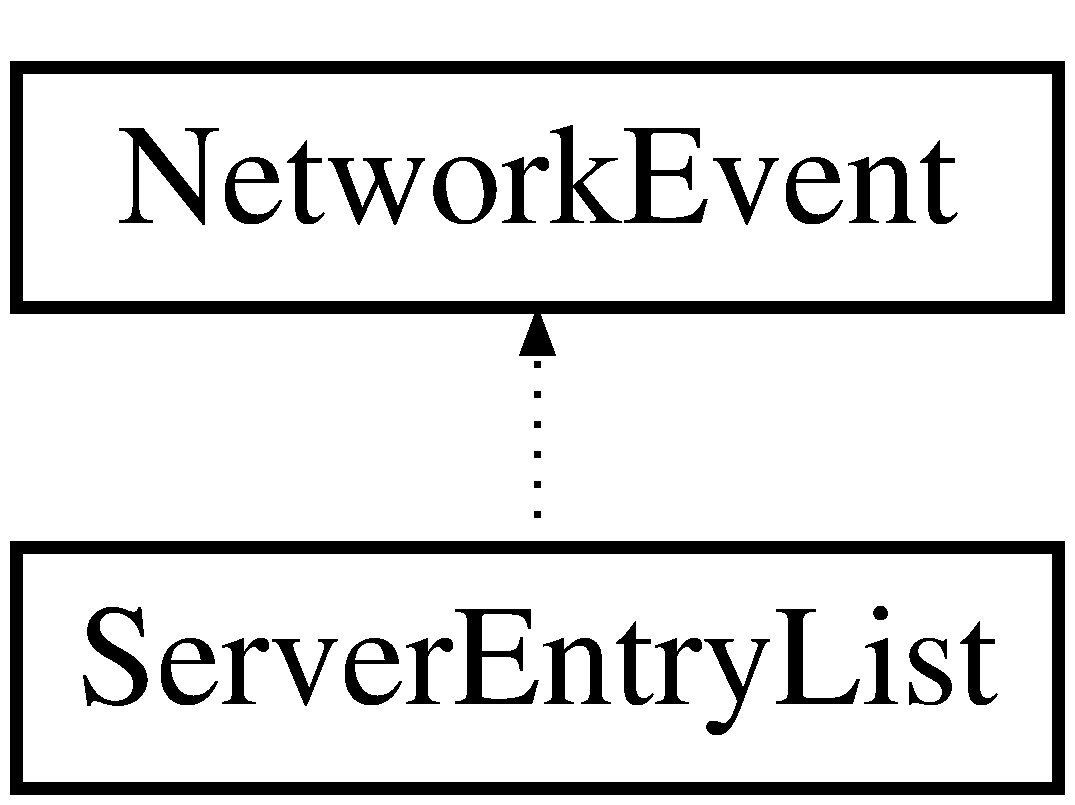
\includegraphics[height=2.000000cm]{class_server_entry_list}
\end{center}
\end{figure}
\subsection*{Public Member Functions}
\begin{DoxyCompactItemize}
\item 
\hypertarget{class_server_entry_list_a1de6a684d051455cb01b5a7463450174}{virtual sf\-::\-Int32 {\bfseries get\-Command} () const }\label{class_server_entry_list_a1de6a684d051455cb01b5a7463450174}

\item 
\hypertarget{class_server_entry_list_a80512f44909663185973ca5492b9a261}{std\-::string {\bfseries get\-Formatted\-Sting} () const }\label{class_server_entry_list_a80512f44909663185973ca5492b9a261}

\end{DoxyCompactItemize}
\subsection*{Public Attributes}
\begin{DoxyCompactItemize}
\item 
\hypertarget{class_server_entry_list_a52397a6ee52b4126c05c894cd7909ab5}{unsigned int {\bfseries entry\-Count}}\label{class_server_entry_list_a52397a6ee52b4126c05c894cd7909ab5}

\item 
\hypertarget{class_server_entry_list_aeddfb1725e3da990489a6687656e85f0}{std\-::vector$<$ \hyperlink{class_server_entry}{Server\-Entry} $>$ {\bfseries entries}}\label{class_server_entry_list_aeddfb1725e3da990489a6687656e85f0}

\end{DoxyCompactItemize}
\subsection*{Friends}
\begin{DoxyCompactItemize}
\item 
\hypertarget{class_server_entry_list_a2fab4a51441a6a5006735424f9d6104f}{sf\-::\-Packet \& {\bfseries operator$<$$<$} (sf\-::\-Packet \&lhs, const \hyperlink{class_server_entry_list}{Server\-Entry\-List} \&rhs)}\label{class_server_entry_list_a2fab4a51441a6a5006735424f9d6104f}

\item 
\hypertarget{class_server_entry_list_adc41cb94c3337543bb9e1845fac0ba61}{sf\-::\-Packet \& {\bfseries operator$>$$>$} (sf\-::\-Packet \&lhs, \hyperlink{class_server_entry_list}{Server\-Entry\-List} \&rhs)}\label{class_server_entry_list_adc41cb94c3337543bb9e1845fac0ba61}

\end{DoxyCompactItemize}
\subsection*{Additional Inherited Members}


The documentation for this class was generated from the following file\-:\begin{DoxyCompactItemize}
\item 
include/Network\-Events.\-h\end{DoxyCompactItemize}

\hypertarget{class_server_entry_reject}{\section{Server\-Entry\-Reject Class Reference}
\label{class_server_entry_reject}\index{Server\-Entry\-Reject@{Server\-Entry\-Reject}}
}
Inheritance diagram for Server\-Entry\-Reject\-:\begin{figure}[H]
\begin{center}
\leavevmode
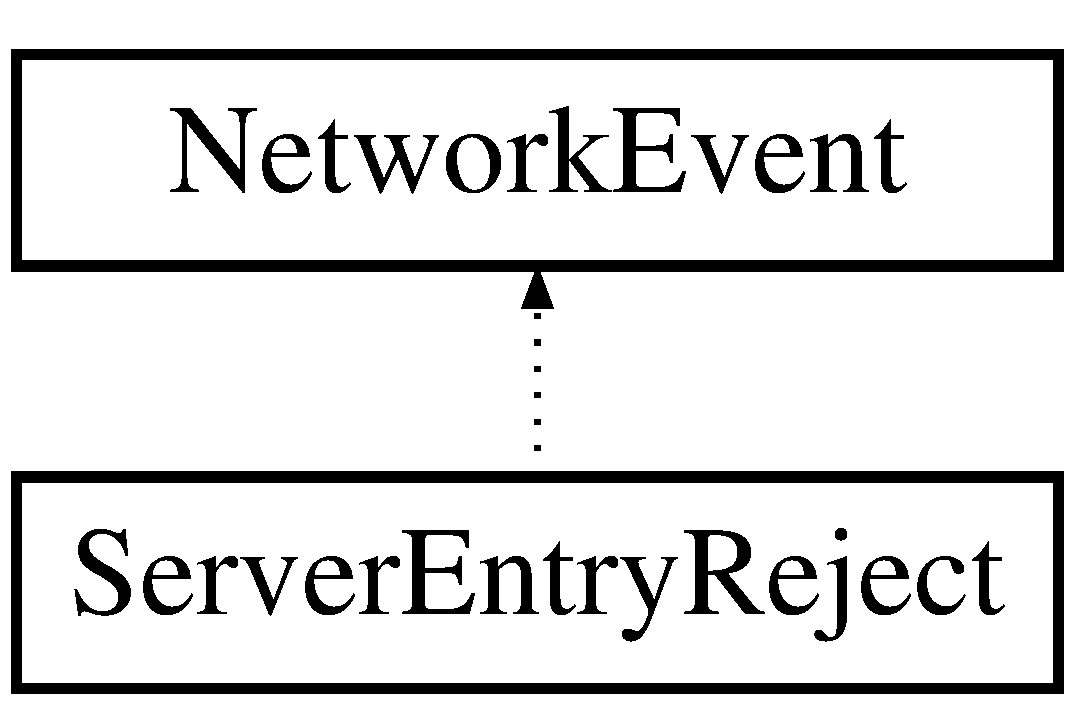
\includegraphics[height=2.000000cm]{class_server_entry_reject}
\end{center}
\end{figure}
\subsection*{Public Member Functions}
\begin{DoxyCompactItemize}
\item 
\hypertarget{class_server_entry_reject_abd4bfbe4de9bd3aabf854719d3cb8e8a}{virtual sf\-::\-Int32 {\bfseries get\-Command} () const }\label{class_server_entry_reject_abd4bfbe4de9bd3aabf854719d3cb8e8a}

\end{DoxyCompactItemize}
\subsection*{Public Attributes}
\begin{DoxyCompactItemize}
\item 
\hypertarget{class_server_entry_reject_ab0963f90b7e8c8f77b152b2540512a15}{std\-::string {\bfseries reason}}\label{class_server_entry_reject_ab0963f90b7e8c8f77b152b2540512a15}

\end{DoxyCompactItemize}
\subsection*{Friends}
\begin{DoxyCompactItemize}
\item 
\hypertarget{class_server_entry_reject_adde98b351cddfab0a69f39e7928f72b5}{sf\-::\-Packet \& {\bfseries operator$<$$<$} (sf\-::\-Packet \&lhs, const \hyperlink{class_server_entry_reject}{Server\-Entry\-Reject} \&rhs)}\label{class_server_entry_reject_adde98b351cddfab0a69f39e7928f72b5}

\item 
\hypertarget{class_server_entry_reject_aa17dcc33d7bcb214f3ee597ac8119bb8}{sf\-::\-Packet \& {\bfseries operator$>$$>$} (sf\-::\-Packet \&lhs, \hyperlink{class_server_entry_reject}{Server\-Entry\-Reject} \&rhs)}\label{class_server_entry_reject_aa17dcc33d7bcb214f3ee597ac8119bb8}

\end{DoxyCompactItemize}
\subsection*{Additional Inherited Members}


The documentation for this class was generated from the following file\-:\begin{DoxyCompactItemize}
\item 
include/Network\-Events.\-h\end{DoxyCompactItemize}

\hypertarget{struct_sorter_record}{\section{Sorter\-Record Struct Reference}
\label{struct_sorter_record}\index{Sorter\-Record@{Sorter\-Record}}
}
\subsection*{Public Attributes}
\begin{DoxyCompactItemize}
\item 
\hypertarget{struct_sorter_record_af59daa686859ca44f7f0be92b3f0d133}{void $\ast$ {\bfseries p\-Val}}\label{struct_sorter_record_af59daa686859ca44f7f0be92b3f0d133}

\item 
\hypertarget{struct_sorter_record_a2b8ffc0f8410826de8b41425759bf462}{int {\bfseries n\-Val}}\label{struct_sorter_record_a2b8ffc0f8410826de8b41425759bf462}

\item 
\hypertarget{struct_sorter_record_a08fdaa8302834166f6a8d12e09c95b58}{\hyperlink{struct_sorter_record}{Sorter\-Record} $\ast$ {\bfseries p\-Next}}\label{struct_sorter_record_a08fdaa8302834166f6a8d12e09c95b58}

\end{DoxyCompactItemize}


The documentation for this struct was generated from the following file\-:\begin{DoxyCompactItemize}
\item 
src/sqlite3.\-c\end{DoxyCompactItemize}

\hypertarget{structsqlite3}{\section{sqlite3 Struct Reference}
\label{structsqlite3}\index{sqlite3@{sqlite3}}
}
\subsection*{Classes}
\begin{DoxyCompactItemize}
\item 
struct \hyperlink{structsqlite3_1_1sqlite3_init_info}{sqlite3\-Init\-Info}
\end{DoxyCompactItemize}
\subsection*{Public Attributes}
\begin{DoxyCompactItemize}
\item 
\hypertarget{structsqlite3_a8ad0bcb473e4cb492165739acff918cd}{\hyperlink{structsqlite3__vfs}{sqlite3\-\_\-vfs} $\ast$ {\bfseries p\-Vfs}}\label{structsqlite3_a8ad0bcb473e4cb492165739acff918cd}

\item 
\hypertarget{structsqlite3_a596f0301f43c5e25575c2a1403f8b571}{struct \hyperlink{struct_vdbe}{Vdbe} $\ast$ {\bfseries p\-Vdbe}}\label{structsqlite3_a596f0301f43c5e25575c2a1403f8b571}

\item 
\hypertarget{structsqlite3_a2e5d7e7ac07c33b11c936b181d07789a}{\hyperlink{struct_coll_seq}{Coll\-Seq} $\ast$ {\bfseries p\-Dflt\-Coll}}\label{structsqlite3_a2e5d7e7ac07c33b11c936b181d07789a}

\item 
\hypertarget{structsqlite3_a6328497ac0393204ab5f5083f05731c9}{\hyperlink{structsqlite3__mutex}{sqlite3\-\_\-mutex} $\ast$ {\bfseries mutex}}\label{structsqlite3_a6328497ac0393204ab5f5083f05731c9}

\item 
\hypertarget{structsqlite3_a0abe1dccdea5f43e6c49360b42749697}{\hyperlink{struct_db}{Db} $\ast$ {\bfseries a\-Db}}\label{structsqlite3_a0abe1dccdea5f43e6c49360b42749697}

\item 
\hypertarget{structsqlite3_a03d047bc289999b0e39d8637f0762489}{int {\bfseries n\-Db}}\label{structsqlite3_a03d047bc289999b0e39d8637f0762489}

\item 
\hypertarget{structsqlite3_a8dac784e669d6b8a9f936d3193c1aaec}{int {\bfseries flags}}\label{structsqlite3_a8dac784e669d6b8a9f936d3193c1aaec}

\item 
\hypertarget{structsqlite3_a9fff52fc4eb087fbb3e3271994fa5198}{i64 {\bfseries last\-Rowid}}\label{structsqlite3_a9fff52fc4eb087fbb3e3271994fa5198}

\item 
\hypertarget{structsqlite3_acfe8618d03dcd195a992886079c3b014}{unsigned int {\bfseries open\-Flags}}\label{structsqlite3_acfe8618d03dcd195a992886079c3b014}

\item 
\hypertarget{structsqlite3_a73adbb5395118bcbd9e4d705712966a2}{int {\bfseries err\-Code}}\label{structsqlite3_a73adbb5395118bcbd9e4d705712966a2}

\item 
\hypertarget{structsqlite3_a12541dafcf60cfce52fb60f84e42f152}{int {\bfseries err\-Mask}}\label{structsqlite3_a12541dafcf60cfce52fb60f84e42f152}

\item 
\hypertarget{structsqlite3_ad4f903754af81d1e646bf966312f9c37}{u16 {\bfseries db\-Opt\-Flags}}\label{structsqlite3_ad4f903754af81d1e646bf966312f9c37}

\item 
\hypertarget{structsqlite3_a11baf5e051b2e4ea03c5d03c09bb624e}{u8 {\bfseries auto\-Commit}}\label{structsqlite3_a11baf5e051b2e4ea03c5d03c09bb624e}

\item 
\hypertarget{structsqlite3_acc46921b20f505ddce64526cac717af3}{u8 {\bfseries temp\-\_\-store}}\label{structsqlite3_acc46921b20f505ddce64526cac717af3}

\item 
\hypertarget{structsqlite3_a79beb0036337ba7fc2de5ccbb9225935}{u8 {\bfseries malloc\-Failed}}\label{structsqlite3_a79beb0036337ba7fc2de5ccbb9225935}

\item 
\hypertarget{structsqlite3_af21b4bbd0d1cda779f2b9e8262e5deec}{u8 {\bfseries dflt\-Lock\-Mode}}\label{structsqlite3_af21b4bbd0d1cda779f2b9e8262e5deec}

\item 
\hypertarget{structsqlite3_a39dac5c9296edb15a46c458fb273bb11}{signed char {\bfseries next\-Autovac}}\label{structsqlite3_a39dac5c9296edb15a46c458fb273bb11}

\item 
\hypertarget{structsqlite3_ac6c776a68a0ce0cbacfc3c9fa5129252}{u8 {\bfseries suppress\-Err}}\label{structsqlite3_ac6c776a68a0ce0cbacfc3c9fa5129252}

\item 
\hypertarget{structsqlite3_acb957d1be62bc33b9f28201cd6dc4d5a}{u8 {\bfseries vtab\-On\-Conflict}}\label{structsqlite3_acb957d1be62bc33b9f28201cd6dc4d5a}

\item 
\hypertarget{structsqlite3_acaca2a1d41db7b83a0fe8a477bd22d1d}{u8 {\bfseries is\-Transaction\-Savepoint}}\label{structsqlite3_acaca2a1d41db7b83a0fe8a477bd22d1d}

\item 
\hypertarget{structsqlite3_aceb220475d2e2fc37b8bf896128b1f1e}{int {\bfseries next\-Pagesize}}\label{structsqlite3_aceb220475d2e2fc37b8bf896128b1f1e}

\item 
\hypertarget{structsqlite3_ad55cf0f70220c91382bc00b6a9423a0d}{u32 {\bfseries magic}}\label{structsqlite3_ad55cf0f70220c91382bc00b6a9423a0d}

\item 
\hypertarget{structsqlite3_aaafd4eaa11ae4ea51d84ed4564a8d372}{int {\bfseries n\-Change}}\label{structsqlite3_aaafd4eaa11ae4ea51d84ed4564a8d372}

\item 
\hypertarget{structsqlite3_ade95b396eda5eb5929851abb581cff3f}{int {\bfseries n\-Total\-Change}}\label{structsqlite3_ade95b396eda5eb5929851abb581cff3f}

\item 
\hypertarget{structsqlite3_ad8acf663e1619905094c9dfe4125157b}{int {\bfseries a\-Limit} \mbox{[}S\-Q\-L\-I\-T\-E\-\_\-\-N\-\_\-\-L\-I\-M\-I\-T\mbox{]}}\label{structsqlite3_ad8acf663e1619905094c9dfe4125157b}

\item 
\hypertarget{structsqlite3_a14bb7fbfa6b662021069fcdf6b334d70}{struct \hyperlink{structsqlite3_1_1sqlite3_init_info}{sqlite3\-::sqlite3\-Init\-Info} {\bfseries init}}\label{structsqlite3_a14bb7fbfa6b662021069fcdf6b334d70}

\item 
\hypertarget{structsqlite3_ada07202e7fd80f275e2e5063d96b5cb0}{int {\bfseries active\-Vdbe\-Cnt}}\label{structsqlite3_ada07202e7fd80f275e2e5063d96b5cb0}

\item 
\hypertarget{structsqlite3_a632e51f8d35c1e8802639661e2fcd567}{int {\bfseries write\-Vdbe\-Cnt}}\label{structsqlite3_a632e51f8d35c1e8802639661e2fcd567}

\item 
\hypertarget{structsqlite3_a7fe8223a600842ffaf99183b1697a6d6}{int {\bfseries vdbe\-Exec\-Cnt}}\label{structsqlite3_a7fe8223a600842ffaf99183b1697a6d6}

\item 
\hypertarget{structsqlite3_aa57fc38ef27d8fa59221cb5c0e54f7fb}{int {\bfseries n\-Extension}}\label{structsqlite3_aa57fc38ef27d8fa59221cb5c0e54f7fb}

\item 
\hypertarget{structsqlite3_aa97954113d8e35c97f8a3af534703f7b}{void $\ast$$\ast$ {\bfseries a\-Extension}}\label{structsqlite3_aa97954113d8e35c97f8a3af534703f7b}

\item 
\hypertarget{structsqlite3_ae438713860c36ad393eb28702b67fec5}{void($\ast$ {\bfseries x\-Trace} )(void $\ast$, const char $\ast$)}\label{structsqlite3_ae438713860c36ad393eb28702b67fec5}

\item 
\hypertarget{structsqlite3_ae0920576e4e92f1b736255fcfad649d1}{void $\ast$ {\bfseries p\-Trace\-Arg}}\label{structsqlite3_ae0920576e4e92f1b736255fcfad649d1}

\item 
\hypertarget{structsqlite3_aa02bf4f3ffdaf52d43a3668661903ffb}{void($\ast$ {\bfseries x\-Profile} )(void $\ast$, const char $\ast$, u64)}\label{structsqlite3_aa02bf4f3ffdaf52d43a3668661903ffb}

\item 
\hypertarget{structsqlite3_a931c234df9b701c78de38ddf22869062}{void $\ast$ {\bfseries p\-Profile\-Arg}}\label{structsqlite3_a931c234df9b701c78de38ddf22869062}

\item 
\hypertarget{structsqlite3_a355237725d3a535d702815b6ef8be75e}{void $\ast$ {\bfseries p\-Commit\-Arg}}\label{structsqlite3_a355237725d3a535d702815b6ef8be75e}

\item 
\hypertarget{structsqlite3_a1b12d797fb7f9c526ffb6665a7f42203}{int($\ast$ {\bfseries x\-Commit\-Callback} )(void $\ast$)}\label{structsqlite3_a1b12d797fb7f9c526ffb6665a7f42203}

\item 
\hypertarget{structsqlite3_a3215967241f15d4599132a8dc2adfb93}{void $\ast$ {\bfseries p\-Rollback\-Arg}}\label{structsqlite3_a3215967241f15d4599132a8dc2adfb93}

\item 
\hypertarget{structsqlite3_ad09cbc96e3c4e322c1722b8c16b9cf24}{void($\ast$ {\bfseries x\-Rollback\-Callback} )(void $\ast$)}\label{structsqlite3_ad09cbc96e3c4e322c1722b8c16b9cf24}

\item 
\hypertarget{structsqlite3_ab4269aa44fea9906fe94045336f13d2a}{void $\ast$ {\bfseries p\-Update\-Arg}}\label{structsqlite3_ab4269aa44fea9906fe94045336f13d2a}

\item 
\hypertarget{structsqlite3_a9177ce33e670ba38c97046e21482414a}{void($\ast$ {\bfseries x\-Update\-Callback} )(void $\ast$, int, const char $\ast$, const char $\ast$, sqlite\-\_\-int64)}\label{structsqlite3_a9177ce33e670ba38c97046e21482414a}

\item 
\hypertarget{structsqlite3_a895ca1f1d541060f1a43ac0267ab6437}{int($\ast$ {\bfseries x\-Wal\-Callback} )(void $\ast$, \hyperlink{structsqlite3}{sqlite3} $\ast$, const char $\ast$, int)}\label{structsqlite3_a895ca1f1d541060f1a43ac0267ab6437}

\item 
\hypertarget{structsqlite3_aa75309c2e522cf0f6ccbd7a3c38e1075}{void $\ast$ {\bfseries p\-Wal\-Arg}}\label{structsqlite3_aa75309c2e522cf0f6ccbd7a3c38e1075}

\item 
\hypertarget{structsqlite3_ac43395ff160433e9811951232b1f6e63}{void($\ast$ {\bfseries x\-Coll\-Needed} )(void $\ast$, \hyperlink{structsqlite3}{sqlite3} $\ast$, int e\-Text\-Rep, const char $\ast$)}\label{structsqlite3_ac43395ff160433e9811951232b1f6e63}

\item 
\hypertarget{structsqlite3_a6401c0e45eb82417cae62b8c5a6425f6}{void($\ast$ {\bfseries x\-Coll\-Needed16} )(void $\ast$, \hyperlink{structsqlite3}{sqlite3} $\ast$, int e\-Text\-Rep, const void $\ast$)}\label{structsqlite3_a6401c0e45eb82417cae62b8c5a6425f6}

\item 
\hypertarget{structsqlite3_addbc9c709cc728968132af5487d5c30c}{void $\ast$ {\bfseries p\-Coll\-Needed\-Arg}}\label{structsqlite3_addbc9c709cc728968132af5487d5c30c}

\item 
\hypertarget{structsqlite3_a90941a0c05641f623c257a7a65b22809}{\hyperlink{struct_mem}{sqlite3\-\_\-value} $\ast$ {\bfseries p\-Err}}\label{structsqlite3_a90941a0c05641f623c257a7a65b22809}

\item 
\hypertarget{structsqlite3_a6227734abcc20349f2964c79cc267860}{char $\ast$ {\bfseries z\-Err\-Msg}}\label{structsqlite3_a6227734abcc20349f2964c79cc267860}

\item 
\hypertarget{structsqlite3_ac127667e438cda63969cc5f027522be1}{char $\ast$ {\bfseries z\-Err\-Msg16}}\label{structsqlite3_ac127667e438cda63969cc5f027522be1}

\item 
\hypertarget{structsqlite3_aec5f477e7fa151f13945251bb4c61497}{\begin{tabbing}
xx\=xx\=xx\=xx\=xx\=xx\=xx\=xx\=xx\=\kill
union \{\\
\>volatile int {\bfseries isInterrupted}\\
\>double {\bfseries notUsed1}\\
\} {\bfseries u1}}\label{structsqlite3_aec5f477e7fa151f13945251bb4c61497}
\\

\end{tabbing}\item 
\hypertarget{structsqlite3_a8a42788add62e1a59d0c930ecc190e87}{\hyperlink{struct_lookaside}{Lookaside} {\bfseries lookaside}}\label{structsqlite3_a8a42788add62e1a59d0c930ecc190e87}

\item 
\hypertarget{structsqlite3_a7eb4472cad41b37417fcc6d2cc0561fa}{int($\ast$ {\bfseries x\-Auth} )(void $\ast$, int, const char $\ast$, const char $\ast$, const char $\ast$, const char $\ast$)}\label{structsqlite3_a7eb4472cad41b37417fcc6d2cc0561fa}

\item 
\hypertarget{structsqlite3_a1c50e81c5e4a6e1faeea93489accd53f}{void $\ast$ {\bfseries p\-Auth\-Arg}}\label{structsqlite3_a1c50e81c5e4a6e1faeea93489accd53f}

\item 
\hypertarget{structsqlite3_aa691b02e7878f45a7c2b59a70e9c5ef3}{int($\ast$ {\bfseries x\-Progress} )(void $\ast$)}\label{structsqlite3_aa691b02e7878f45a7c2b59a70e9c5ef3}

\item 
\hypertarget{structsqlite3_a1731a4d0a73f57415d35ef2a2997971b}{void $\ast$ {\bfseries p\-Progress\-Arg}}\label{structsqlite3_a1731a4d0a73f57415d35ef2a2997971b}

\item 
\hypertarget{structsqlite3_af124e2c511fea75ead3b1f180ce63447}{int {\bfseries n\-Progress\-Ops}}\label{structsqlite3_af124e2c511fea75ead3b1f180ce63447}

\item 
\hypertarget{structsqlite3_a895162274d29fcd0658901bc5dcce99b}{int {\bfseries n\-V\-Trans}}\label{structsqlite3_a895162274d29fcd0658901bc5dcce99b}

\item 
\hypertarget{structsqlite3_a1e03e1fdee6fb7cb7337628c7f9b37c4}{\hyperlink{struct_hash}{Hash} {\bfseries a\-Module}}\label{structsqlite3_a1e03e1fdee6fb7cb7337628c7f9b37c4}

\item 
\hypertarget{structsqlite3_a6c0dc858220431633ce44351a6ce2962}{\hyperlink{struct_vtab_ctx}{Vtab\-Ctx} $\ast$ {\bfseries p\-Vtab\-Ctx}}\label{structsqlite3_a6c0dc858220431633ce44351a6ce2962}

\item 
\hypertarget{structsqlite3_a9628b6da0f4c7dbde32dcd1249d6a712}{\hyperlink{struct_v_table}{V\-Table} $\ast$$\ast$ {\bfseries a\-V\-Trans}}\label{structsqlite3_a9628b6da0f4c7dbde32dcd1249d6a712}

\item 
\hypertarget{structsqlite3_a048405f503316fad7d7116fd930299db}{\hyperlink{struct_v_table}{V\-Table} $\ast$ {\bfseries p\-Disconnect}}\label{structsqlite3_a048405f503316fad7d7116fd930299db}

\item 
\hypertarget{structsqlite3_a1f1c623a26e916021fbb2fe6d84dcede}{\hyperlink{struct_func_def_hash}{Func\-Def\-Hash} {\bfseries a\-Func}}\label{structsqlite3_a1f1c623a26e916021fbb2fe6d84dcede}

\item 
\hypertarget{structsqlite3_a259afda236b21b947f6dc7e0b3e605c3}{\hyperlink{struct_hash}{Hash} {\bfseries a\-Coll\-Seq}}\label{structsqlite3_a259afda236b21b947f6dc7e0b3e605c3}

\item 
\hypertarget{structsqlite3_a5f50915803efe2ad40dc1a5e31763671}{\hyperlink{struct_busy_handler}{Busy\-Handler} {\bfseries busy\-Handler}}\label{structsqlite3_a5f50915803efe2ad40dc1a5e31763671}

\item 
\hypertarget{structsqlite3_ad99069213dff7fede71447b97d22d710}{\hyperlink{struct_db}{Db} {\bfseries a\-Db\-Static} \mbox{[}2\mbox{]}}\label{structsqlite3_ad99069213dff7fede71447b97d22d710}

\item 
\hypertarget{structsqlite3_a47f4fe21bba981ccd47ee7f873f48a07}{\hyperlink{struct_savepoint}{Savepoint} $\ast$ {\bfseries p\-Savepoint}}\label{structsqlite3_a47f4fe21bba981ccd47ee7f873f48a07}

\item 
\hypertarget{structsqlite3_a69237f7a2b079706c544f09255fd8905}{int {\bfseries busy\-Timeout}}\label{structsqlite3_a69237f7a2b079706c544f09255fd8905}

\item 
\hypertarget{structsqlite3_a51d1dc4f5668dbc2282162bdfdca96ec}{int {\bfseries n\-Savepoint}}\label{structsqlite3_a51d1dc4f5668dbc2282162bdfdca96ec}

\item 
\hypertarget{structsqlite3_a727c6da42aa4313c715de350303c90f6}{int {\bfseries n\-Statement}}\label{structsqlite3_a727c6da42aa4313c715de350303c90f6}

\item 
\hypertarget{structsqlite3_a1d74627daa6fe93811e99cffe9362c10}{i64 {\bfseries n\-Deferred\-Cons}}\label{structsqlite3_a1d74627daa6fe93811e99cffe9362c10}

\item 
\hypertarget{structsqlite3_a5559fb199b06ee59b635bb18f153fcf8}{int $\ast$ {\bfseries pn\-Bytes\-Freed}}\label{structsqlite3_a5559fb199b06ee59b635bb18f153fcf8}

\end{DoxyCompactItemize}


The documentation for this struct was generated from the following file\-:\begin{DoxyCompactItemize}
\item 
src/sqlite3.\-c\end{DoxyCompactItemize}

\hypertarget{structsqlite3__api__routines}{\section{sqlite3\-\_\-api\-\_\-routines Struct Reference}
\label{structsqlite3__api__routines}\index{sqlite3\-\_\-api\-\_\-routines@{sqlite3\-\_\-api\-\_\-routines}}
}
\subsection*{Public Attributes}
\begin{DoxyCompactItemize}
\item 
\hypertarget{structsqlite3__api__routines_a16fafb5f2460657f528338aee5f65d25}{void $\ast$($\ast$ {\bfseries aggregate\-\_\-context} )(\hyperlink{structsqlite3__context}{sqlite3\-\_\-context} $\ast$, int n\-Bytes)}\label{structsqlite3__api__routines_a16fafb5f2460657f528338aee5f65d25}

\item 
\hypertarget{structsqlite3__api__routines_a8373f7a5dd2d6f1c86bbf024b1796156}{int($\ast$ {\bfseries aggregate\-\_\-count} )(\hyperlink{structsqlite3__context}{sqlite3\-\_\-context} $\ast$)}\label{structsqlite3__api__routines_a8373f7a5dd2d6f1c86bbf024b1796156}

\item 
\hypertarget{structsqlite3__api__routines_afeb41d70ab5a221fec488560934c825b}{int($\ast$ {\bfseries bind\-\_\-blob} )(sqlite3\-\_\-stmt $\ast$, int, const void $\ast$, int n, void($\ast$)(void $\ast$))}\label{structsqlite3__api__routines_afeb41d70ab5a221fec488560934c825b}

\item 
\hypertarget{structsqlite3__api__routines_aca43a229ce28397ba8c18a4d6e03e40c}{int($\ast$ {\bfseries bind\-\_\-double} )(sqlite3\-\_\-stmt $\ast$, int, double)}\label{structsqlite3__api__routines_aca43a229ce28397ba8c18a4d6e03e40c}

\item 
\hypertarget{structsqlite3__api__routines_a6fef49e6c9c1fa573c55cc6668a8448f}{int($\ast$ {\bfseries bind\-\_\-int} )(sqlite3\-\_\-stmt $\ast$, int, int)}\label{structsqlite3__api__routines_a6fef49e6c9c1fa573c55cc6668a8448f}

\item 
\hypertarget{structsqlite3__api__routines_a489304cada65abca390da9b751da8800}{int($\ast$ {\bfseries bind\-\_\-int64} )(sqlite3\-\_\-stmt $\ast$, int, sqlite\-\_\-int64)}\label{structsqlite3__api__routines_a489304cada65abca390da9b751da8800}

\item 
\hypertarget{structsqlite3__api__routines_a74d16d0bb57db37d654e95fb7e72c93c}{int($\ast$ {\bfseries bind\-\_\-null} )(sqlite3\-\_\-stmt $\ast$, int)}\label{structsqlite3__api__routines_a74d16d0bb57db37d654e95fb7e72c93c}

\item 
\hypertarget{structsqlite3__api__routines_ab27285b7fb132f697d5ef22f21469dd6}{int($\ast$ {\bfseries bind\-\_\-parameter\-\_\-count} )(sqlite3\-\_\-stmt $\ast$)}\label{structsqlite3__api__routines_ab27285b7fb132f697d5ef22f21469dd6}

\item 
\hypertarget{structsqlite3__api__routines_a1985681b1e13047a8aae17676debb39d}{int($\ast$ {\bfseries bind\-\_\-parameter\-\_\-index} )(sqlite3\-\_\-stmt $\ast$, const char $\ast$z\-Name)}\label{structsqlite3__api__routines_a1985681b1e13047a8aae17676debb39d}

\item 
\hypertarget{structsqlite3__api__routines_aff41be2d08dbacf60407b53567d6bead}{const char $\ast$($\ast$ {\bfseries bind\-\_\-parameter\-\_\-name} )(sqlite3\-\_\-stmt $\ast$, int)}\label{structsqlite3__api__routines_aff41be2d08dbacf60407b53567d6bead}

\item 
\hypertarget{structsqlite3__api__routines_a4e64c1e01f7317ce0924683bf26b165a}{int($\ast$ {\bfseries bind\-\_\-text} )(sqlite3\-\_\-stmt $\ast$, int, const char $\ast$, int n, void($\ast$)(void $\ast$))}\label{structsqlite3__api__routines_a4e64c1e01f7317ce0924683bf26b165a}

\item 
\hypertarget{structsqlite3__api__routines_a4613c5fa0a1fac009914ddd0f4415cfd}{int($\ast$ {\bfseries bind\-\_\-text16} )(sqlite3\-\_\-stmt $\ast$, int, const void $\ast$, int, void($\ast$)(void $\ast$))}\label{structsqlite3__api__routines_a4613c5fa0a1fac009914ddd0f4415cfd}

\item 
\hypertarget{structsqlite3__api__routines_aca47715615cc037cd2f850e8c87cd68d}{int($\ast$ {\bfseries bind\-\_\-value} )(sqlite3\-\_\-stmt $\ast$, int, const \hyperlink{struct_mem}{sqlite3\-\_\-value} $\ast$)}\label{structsqlite3__api__routines_aca47715615cc037cd2f850e8c87cd68d}

\item 
\hypertarget{structsqlite3__api__routines_a4dd578712242bb36acf8568f1c0da278}{int($\ast$ {\bfseries busy\-\_\-handler} )(\hyperlink{structsqlite3}{sqlite3} $\ast$, int($\ast$)(void $\ast$, int), void $\ast$)}\label{structsqlite3__api__routines_a4dd578712242bb36acf8568f1c0da278}

\item 
\hypertarget{structsqlite3__api__routines_a403a82d983e3a60444761e4f78d6269c}{int($\ast$ {\bfseries busy\-\_\-timeout} )(\hyperlink{structsqlite3}{sqlite3} $\ast$, int ms)}\label{structsqlite3__api__routines_a403a82d983e3a60444761e4f78d6269c}

\item 
\hypertarget{structsqlite3__api__routines_a1379bef0cb6e5e352dc26a34e2d02477}{int($\ast$ {\bfseries changes} )(\hyperlink{structsqlite3}{sqlite3} $\ast$)}\label{structsqlite3__api__routines_a1379bef0cb6e5e352dc26a34e2d02477}

\item 
\hypertarget{structsqlite3__api__routines_a26f93f921a5f6709be46902616ca8bcf}{int($\ast$ {\bfseries close} )(\hyperlink{structsqlite3}{sqlite3} $\ast$)}\label{structsqlite3__api__routines_a26f93f921a5f6709be46902616ca8bcf}

\item 
\hypertarget{structsqlite3__api__routines_aa26fb10907a304b5afd943061dd08ab7}{int($\ast$ {\bfseries collation\-\_\-needed} )(\hyperlink{structsqlite3}{sqlite3} $\ast$, void $\ast$, void($\ast$)(void $\ast$, \hyperlink{structsqlite3}{sqlite3} $\ast$, int e\-Text\-Rep, const char $\ast$))}\label{structsqlite3__api__routines_aa26fb10907a304b5afd943061dd08ab7}

\item 
\hypertarget{structsqlite3__api__routines_a35eb5a4b4df8b310e5e9ffbaa735d38f}{int($\ast$ {\bfseries collation\-\_\-needed16} )(\hyperlink{structsqlite3}{sqlite3} $\ast$, void $\ast$, void($\ast$)(void $\ast$, \hyperlink{structsqlite3}{sqlite3} $\ast$, int e\-Text\-Rep, const void $\ast$))}\label{structsqlite3__api__routines_a35eb5a4b4df8b310e5e9ffbaa735d38f}

\item 
\hypertarget{structsqlite3__api__routines_a66f2cefdf5bef54891cbef548f91c781}{const void $\ast$($\ast$ {\bfseries column\-\_\-blob} )(sqlite3\-\_\-stmt $\ast$, int i\-Col)}\label{structsqlite3__api__routines_a66f2cefdf5bef54891cbef548f91c781}

\item 
\hypertarget{structsqlite3__api__routines_a79150244afb5f778840bc9df72d55342}{int($\ast$ {\bfseries column\-\_\-bytes} )(sqlite3\-\_\-stmt $\ast$, int i\-Col)}\label{structsqlite3__api__routines_a79150244afb5f778840bc9df72d55342}

\item 
\hypertarget{structsqlite3__api__routines_ac1daf0a08de4a33c8db27a29f13a26ad}{int($\ast$ {\bfseries column\-\_\-bytes16} )(sqlite3\-\_\-stmt $\ast$, int i\-Col)}\label{structsqlite3__api__routines_ac1daf0a08de4a33c8db27a29f13a26ad}

\item 
\hypertarget{structsqlite3__api__routines_af750a4727dc59edb4ad2933e28bfa358}{int($\ast$ {\bfseries column\-\_\-count} )(sqlite3\-\_\-stmt $\ast$p\-Stmt)}\label{structsqlite3__api__routines_af750a4727dc59edb4ad2933e28bfa358}

\item 
\hypertarget{structsqlite3__api__routines_a7b8e1de81b22244eab04e90ebed49bf5}{const char $\ast$($\ast$ {\bfseries column\-\_\-database\-\_\-name} )(sqlite3\-\_\-stmt $\ast$, int)}\label{structsqlite3__api__routines_a7b8e1de81b22244eab04e90ebed49bf5}

\item 
\hypertarget{structsqlite3__api__routines_af8e642aae1dd0f81828eaa7759791fe9}{const void $\ast$($\ast$ {\bfseries column\-\_\-database\-\_\-name16} )(sqlite3\-\_\-stmt $\ast$, int)}\label{structsqlite3__api__routines_af8e642aae1dd0f81828eaa7759791fe9}

\item 
\hypertarget{structsqlite3__api__routines_aad9e3c9907f96de1d4db36839e98ec01}{const char $\ast$($\ast$ {\bfseries column\-\_\-decltype} )(sqlite3\-\_\-stmt $\ast$, int i)}\label{structsqlite3__api__routines_aad9e3c9907f96de1d4db36839e98ec01}

\item 
\hypertarget{structsqlite3__api__routines_aa0c2e3c8ba3face8a9ca7825fa2abac1}{const void $\ast$($\ast$ {\bfseries column\-\_\-decltype16} )(sqlite3\-\_\-stmt $\ast$, int)}\label{structsqlite3__api__routines_aa0c2e3c8ba3face8a9ca7825fa2abac1}

\item 
\hypertarget{structsqlite3__api__routines_afd21003df28cb46354c00599b90e6de5}{double($\ast$ {\bfseries column\-\_\-double} )(sqlite3\-\_\-stmt $\ast$, int i\-Col)}\label{structsqlite3__api__routines_afd21003df28cb46354c00599b90e6de5}

\item 
\hypertarget{structsqlite3__api__routines_a6211d95cf114f26cb48eed02d3b5eb70}{int($\ast$ {\bfseries column\-\_\-int} )(sqlite3\-\_\-stmt $\ast$, int i\-Col)}\label{structsqlite3__api__routines_a6211d95cf114f26cb48eed02d3b5eb70}

\item 
\hypertarget{structsqlite3__api__routines_a523a8d125fe83c9ea45eb4057a4d2458}{sqlite\-\_\-int64($\ast$ {\bfseries column\-\_\-int64} )(sqlite3\-\_\-stmt $\ast$, int i\-Col)}\label{structsqlite3__api__routines_a523a8d125fe83c9ea45eb4057a4d2458}

\item 
\hypertarget{structsqlite3__api__routines_ab01499e4ca8ec6db92f34f8274041ae5}{const char $\ast$($\ast$ {\bfseries column\-\_\-name} )(sqlite3\-\_\-stmt $\ast$, int)}\label{structsqlite3__api__routines_ab01499e4ca8ec6db92f34f8274041ae5}

\item 
\hypertarget{structsqlite3__api__routines_a4ca83aec1d4cfe474f1afa0bcdde0e20}{const void $\ast$($\ast$ {\bfseries column\-\_\-name16} )(sqlite3\-\_\-stmt $\ast$, int)}\label{structsqlite3__api__routines_a4ca83aec1d4cfe474f1afa0bcdde0e20}

\item 
\hypertarget{structsqlite3__api__routines_a18cb726aaf966e6d4a6954cb3c716991}{const char $\ast$($\ast$ {\bfseries column\-\_\-origin\-\_\-name} )(sqlite3\-\_\-stmt $\ast$, int)}\label{structsqlite3__api__routines_a18cb726aaf966e6d4a6954cb3c716991}

\item 
\hypertarget{structsqlite3__api__routines_ae5022cdbd16222eaf08d5fdba9292142}{const void $\ast$($\ast$ {\bfseries column\-\_\-origin\-\_\-name16} )(sqlite3\-\_\-stmt $\ast$, int)}\label{structsqlite3__api__routines_ae5022cdbd16222eaf08d5fdba9292142}

\item 
\hypertarget{structsqlite3__api__routines_a66cc9e4b3cb918a699f3386df76ed1bc}{const char $\ast$($\ast$ {\bfseries column\-\_\-table\-\_\-name} )(sqlite3\-\_\-stmt $\ast$, int)}\label{structsqlite3__api__routines_a66cc9e4b3cb918a699f3386df76ed1bc}

\item 
\hypertarget{structsqlite3__api__routines_a9b19d2cacecce0a09c5bdcffc6e44197}{const void $\ast$($\ast$ {\bfseries column\-\_\-table\-\_\-name16} )(sqlite3\-\_\-stmt $\ast$, int)}\label{structsqlite3__api__routines_a9b19d2cacecce0a09c5bdcffc6e44197}

\item 
\hypertarget{structsqlite3__api__routines_a0857bdde632d86319b569c64668bed69}{const unsigned char $\ast$($\ast$ {\bfseries column\-\_\-text} )(sqlite3\-\_\-stmt $\ast$, int i\-Col)}\label{structsqlite3__api__routines_a0857bdde632d86319b569c64668bed69}

\item 
\hypertarget{structsqlite3__api__routines_a893fc55c1762d1bb927d4821a1340dd9}{const void $\ast$($\ast$ {\bfseries column\-\_\-text16} )(sqlite3\-\_\-stmt $\ast$, int i\-Col)}\label{structsqlite3__api__routines_a893fc55c1762d1bb927d4821a1340dd9}

\item 
\hypertarget{structsqlite3__api__routines_a1bfa18703e814caf9b940bd89247fde5}{int($\ast$ {\bfseries column\-\_\-type} )(sqlite3\-\_\-stmt $\ast$, int i\-Col)}\label{structsqlite3__api__routines_a1bfa18703e814caf9b940bd89247fde5}

\item 
\hypertarget{structsqlite3__api__routines_a051de47b5f1331319af6b6c9062e8b32}{\hyperlink{struct_mem}{sqlite3\-\_\-value} $\ast$($\ast$ {\bfseries column\-\_\-value} )(sqlite3\-\_\-stmt $\ast$, int i\-Col)}\label{structsqlite3__api__routines_a051de47b5f1331319af6b6c9062e8b32}

\item 
\hypertarget{structsqlite3__api__routines_a7a0ba7cc6db07bf2d0db7e0d5234095f}{void $\ast$($\ast$ {\bfseries commit\-\_\-hook} )(\hyperlink{structsqlite3}{sqlite3} $\ast$, int($\ast$)(void $\ast$), void $\ast$)}\label{structsqlite3__api__routines_a7a0ba7cc6db07bf2d0db7e0d5234095f}

\item 
\hypertarget{structsqlite3__api__routines_a4bd1a90b2a40c58ecc1c2ceb67be48f5}{int($\ast$ {\bfseries complete} )(const char $\ast$sql)}\label{structsqlite3__api__routines_a4bd1a90b2a40c58ecc1c2ceb67be48f5}

\item 
\hypertarget{structsqlite3__api__routines_ae3e27f61b6c43cf549360f1bb8b3b591}{int($\ast$ {\bfseries complete16} )(const void $\ast$sql)}\label{structsqlite3__api__routines_ae3e27f61b6c43cf549360f1bb8b3b591}

\item 
\hypertarget{structsqlite3__api__routines_aed840be5b7cc7add4f21ba88f1981f58}{int($\ast$ {\bfseries create\-\_\-collation} )(\hyperlink{structsqlite3}{sqlite3} $\ast$, const char $\ast$, int, void $\ast$, int($\ast$)(void $\ast$, int, const void $\ast$, int, const void $\ast$))}\label{structsqlite3__api__routines_aed840be5b7cc7add4f21ba88f1981f58}

\item 
\hypertarget{structsqlite3__api__routines_a2f05772713bb942bff670352a96ee1e6}{int($\ast$ {\bfseries create\-\_\-collation16} )(\hyperlink{structsqlite3}{sqlite3} $\ast$, const void $\ast$, int, void $\ast$, int($\ast$)(void $\ast$, int, const void $\ast$, int, const void $\ast$))}\label{structsqlite3__api__routines_a2f05772713bb942bff670352a96ee1e6}

\item 
\hypertarget{structsqlite3__api__routines_aaf30781efad4fb70111f391e6fe20a9c}{int($\ast$ {\bfseries create\-\_\-function} )(\hyperlink{structsqlite3}{sqlite3} $\ast$, const char $\ast$, int, int, void $\ast$, void($\ast$x\-Func)(\hyperlink{structsqlite3__context}{sqlite3\-\_\-context} $\ast$, int, \hyperlink{struct_mem}{sqlite3\-\_\-value} $\ast$$\ast$), void($\ast$x\-Step)(\hyperlink{structsqlite3__context}{sqlite3\-\_\-context} $\ast$, int, \hyperlink{struct_mem}{sqlite3\-\_\-value} $\ast$$\ast$), void($\ast$x\-Final)(\hyperlink{structsqlite3__context}{sqlite3\-\_\-context} $\ast$))}\label{structsqlite3__api__routines_aaf30781efad4fb70111f391e6fe20a9c}

\item 
\hypertarget{structsqlite3__api__routines_a0c3f05b118b89293ff5d35774504b44d}{int($\ast$ {\bfseries create\-\_\-function16} )(\hyperlink{structsqlite3}{sqlite3} $\ast$, const void $\ast$, int, int, void $\ast$, void($\ast$x\-Func)(\hyperlink{structsqlite3__context}{sqlite3\-\_\-context} $\ast$, int, \hyperlink{struct_mem}{sqlite3\-\_\-value} $\ast$$\ast$), void($\ast$x\-Step)(\hyperlink{structsqlite3__context}{sqlite3\-\_\-context} $\ast$, int, \hyperlink{struct_mem}{sqlite3\-\_\-value} $\ast$$\ast$), void($\ast$x\-Final)(\hyperlink{structsqlite3__context}{sqlite3\-\_\-context} $\ast$))}\label{structsqlite3__api__routines_a0c3f05b118b89293ff5d35774504b44d}

\item 
\hypertarget{structsqlite3__api__routines_a25834b37191417562ecd2ee67b85617b}{int($\ast$ {\bfseries create\-\_\-module} )(\hyperlink{structsqlite3}{sqlite3} $\ast$, const char $\ast$, const \hyperlink{structsqlite3__module}{sqlite3\-\_\-module} $\ast$, void $\ast$)}\label{structsqlite3__api__routines_a25834b37191417562ecd2ee67b85617b}

\item 
\hypertarget{structsqlite3__api__routines_aea0a7b7483770202ef9eae88b4eb70cd}{int($\ast$ {\bfseries data\-\_\-count} )(sqlite3\-\_\-stmt $\ast$p\-Stmt)}\label{structsqlite3__api__routines_aea0a7b7483770202ef9eae88b4eb70cd}

\item 
\hypertarget{structsqlite3__api__routines_ab0133d05f54efba67f6172538ca25ae0}{\hyperlink{structsqlite3}{sqlite3} $\ast$($\ast$ {\bfseries db\-\_\-handle} )(sqlite3\-\_\-stmt $\ast$)}\label{structsqlite3__api__routines_ab0133d05f54efba67f6172538ca25ae0}

\item 
\hypertarget{structsqlite3__api__routines_a6b6035b36ea9d0800181e69e20059b32}{int($\ast$ {\bfseries declare\-\_\-vtab} )(\hyperlink{structsqlite3}{sqlite3} $\ast$, const char $\ast$)}\label{structsqlite3__api__routines_a6b6035b36ea9d0800181e69e20059b32}

\item 
\hypertarget{structsqlite3__api__routines_a3e6b7bbdd68cde43ef4afffd73e957ea}{int($\ast$ {\bfseries enable\-\_\-shared\-\_\-cache} )(int)}\label{structsqlite3__api__routines_a3e6b7bbdd68cde43ef4afffd73e957ea}

\item 
\hypertarget{structsqlite3__api__routines_a0f1cf42108e6d872d03b78eaf27dfc45}{int($\ast$ {\bfseries errcode} )(\hyperlink{structsqlite3}{sqlite3} $\ast$db)}\label{structsqlite3__api__routines_a0f1cf42108e6d872d03b78eaf27dfc45}

\item 
\hypertarget{structsqlite3__api__routines_a953d37f24ded9d93449f1d0eb64b8894}{const char $\ast$($\ast$ {\bfseries errmsg} )(\hyperlink{structsqlite3}{sqlite3} $\ast$)}\label{structsqlite3__api__routines_a953d37f24ded9d93449f1d0eb64b8894}

\item 
\hypertarget{structsqlite3__api__routines_a06f862750a8e1e1b21a942cc483c4f71}{const void $\ast$($\ast$ {\bfseries errmsg16} )(\hyperlink{structsqlite3}{sqlite3} $\ast$)}\label{structsqlite3__api__routines_a06f862750a8e1e1b21a942cc483c4f71}

\item 
\hypertarget{structsqlite3__api__routines_a16e1fe4f9dccfe8da742d7087822d379}{int($\ast$ {\bfseries exec} )(\hyperlink{structsqlite3}{sqlite3} $\ast$, const char $\ast$, sqlite3\-\_\-callback, void $\ast$, char $\ast$$\ast$)}\label{structsqlite3__api__routines_a16e1fe4f9dccfe8da742d7087822d379}

\item 
\hypertarget{structsqlite3__api__routines_a574080049ce24e639e7487bcfc74e06a}{int($\ast$ {\bfseries expired} )(sqlite3\-\_\-stmt $\ast$)}\label{structsqlite3__api__routines_a574080049ce24e639e7487bcfc74e06a}

\item 
\hypertarget{structsqlite3__api__routines_ad7cee4127bfd0583ccfea40943858de2}{int($\ast$ {\bfseries finalize} )(sqlite3\-\_\-stmt $\ast$p\-Stmt)}\label{structsqlite3__api__routines_ad7cee4127bfd0583ccfea40943858de2}

\item 
\hypertarget{structsqlite3__api__routines_a5778783c18a96cff28a516168db77ae9}{void($\ast$ {\bfseries free} )(void $\ast$)}\label{structsqlite3__api__routines_a5778783c18a96cff28a516168db77ae9}

\item 
\hypertarget{structsqlite3__api__routines_a16d39862f10f54f34e2d52b4da51fdac}{void($\ast$ {\bfseries free\-\_\-table} )(char $\ast$$\ast$result)}\label{structsqlite3__api__routines_a16d39862f10f54f34e2d52b4da51fdac}

\item 
\hypertarget{structsqlite3__api__routines_a8724984acc7ccfefaa17f04a739fc396}{int($\ast$ {\bfseries get\-\_\-autocommit} )(\hyperlink{structsqlite3}{sqlite3} $\ast$)}\label{structsqlite3__api__routines_a8724984acc7ccfefaa17f04a739fc396}

\item 
\hypertarget{structsqlite3__api__routines_a1eb728229d0ff6e3bc3c5f25a4058060}{void $\ast$($\ast$ {\bfseries get\-\_\-auxdata} )(\hyperlink{structsqlite3__context}{sqlite3\-\_\-context} $\ast$, int)}\label{structsqlite3__api__routines_a1eb728229d0ff6e3bc3c5f25a4058060}

\item 
\hypertarget{structsqlite3__api__routines_a49be6136a17441b04e3feec330d9dd52}{int($\ast$ {\bfseries get\-\_\-table} )(\hyperlink{structsqlite3}{sqlite3} $\ast$, const char $\ast$, char $\ast$$\ast$$\ast$, int $\ast$, int $\ast$, char $\ast$$\ast$)}\label{structsqlite3__api__routines_a49be6136a17441b04e3feec330d9dd52}

\item 
\hypertarget{structsqlite3__api__routines_a9b90b5ea9b2fae5a60b9ddc86c72e1a8}{int($\ast$ {\bfseries global\-\_\-recover} )(void)}\label{structsqlite3__api__routines_a9b90b5ea9b2fae5a60b9ddc86c72e1a8}

\item 
\hypertarget{structsqlite3__api__routines_a3cfec591003c4e8b1f1bdb82a80b8e19}{void($\ast$ {\bfseries interruptx} )(\hyperlink{structsqlite3}{sqlite3} $\ast$)}\label{structsqlite3__api__routines_a3cfec591003c4e8b1f1bdb82a80b8e19}

\item 
\hypertarget{structsqlite3__api__routines_aeeda8d84c8060c99e24d97ae60bf6046}{sqlite\-\_\-int64($\ast$ {\bfseries last\-\_\-insert\-\_\-rowid} )(\hyperlink{structsqlite3}{sqlite3} $\ast$)}\label{structsqlite3__api__routines_aeeda8d84c8060c99e24d97ae60bf6046}

\item 
\hypertarget{structsqlite3__api__routines_a126a447b5724f50142603d94d9470336}{const char $\ast$($\ast$ {\bfseries libversion} )(void)}\label{structsqlite3__api__routines_a126a447b5724f50142603d94d9470336}

\item 
\hypertarget{structsqlite3__api__routines_a70d0b04a52493c15f26815990a50afa7}{int($\ast$ {\bfseries libversion\-\_\-number} )(void)}\label{structsqlite3__api__routines_a70d0b04a52493c15f26815990a50afa7}

\item 
\hypertarget{structsqlite3__api__routines_a37193f93e0626dae6e302d0bd47de4cf}{void $\ast$($\ast$ {\bfseries malloc} )(int)}\label{structsqlite3__api__routines_a37193f93e0626dae6e302d0bd47de4cf}

\item 
\hypertarget{structsqlite3__api__routines_a82cc01d97e2552bad02554ed50e4d2b8}{char $\ast$($\ast$ {\bfseries mprintf} )(const char $\ast$,...)}\label{structsqlite3__api__routines_a82cc01d97e2552bad02554ed50e4d2b8}

\item 
\hypertarget{structsqlite3__api__routines_a1d0126d7384e1e4e0975d3084007af89}{int($\ast$ {\bfseries open} )(const char $\ast$, \hyperlink{structsqlite3}{sqlite3} $\ast$$\ast$)}\label{structsqlite3__api__routines_a1d0126d7384e1e4e0975d3084007af89}

\item 
\hypertarget{structsqlite3__api__routines_a8394f1e962c0c3172ef7a0b6243303ca}{int($\ast$ {\bfseries open16} )(const void $\ast$, \hyperlink{structsqlite3}{sqlite3} $\ast$$\ast$)}\label{structsqlite3__api__routines_a8394f1e962c0c3172ef7a0b6243303ca}

\item 
\hypertarget{structsqlite3__api__routines_a6d5170ffef9564b7f9b157a14df4fd4d}{int($\ast$ {\bfseries prepare} )(\hyperlink{structsqlite3}{sqlite3} $\ast$, const char $\ast$, int, sqlite3\-\_\-stmt $\ast$$\ast$, const char $\ast$$\ast$)}\label{structsqlite3__api__routines_a6d5170ffef9564b7f9b157a14df4fd4d}

\item 
\hypertarget{structsqlite3__api__routines_a3877cfcfebeb05e357317ab50a47e52e}{int($\ast$ {\bfseries prepare16} )(\hyperlink{structsqlite3}{sqlite3} $\ast$, const void $\ast$, int, sqlite3\-\_\-stmt $\ast$$\ast$, const void $\ast$$\ast$)}\label{structsqlite3__api__routines_a3877cfcfebeb05e357317ab50a47e52e}

\item 
\hypertarget{structsqlite3__api__routines_a2f4fef66c120fa8480e60e60099052e3}{void $\ast$($\ast$ {\bfseries profile} )(\hyperlink{structsqlite3}{sqlite3} $\ast$, void($\ast$)(void $\ast$, const char $\ast$, sqlite\-\_\-uint64), void $\ast$)}\label{structsqlite3__api__routines_a2f4fef66c120fa8480e60e60099052e3}

\item 
\hypertarget{structsqlite3__api__routines_a2888055619addf1d754e25d159d85718}{void($\ast$ {\bfseries progress\-\_\-handler} )(\hyperlink{structsqlite3}{sqlite3} $\ast$, int, int($\ast$)(void $\ast$), void $\ast$)}\label{structsqlite3__api__routines_a2888055619addf1d754e25d159d85718}

\item 
\hypertarget{structsqlite3__api__routines_afd935ceb7b7519dfc04ad9e05254a2c9}{void $\ast$($\ast$ {\bfseries realloc} )(void $\ast$, int)}\label{structsqlite3__api__routines_afd935ceb7b7519dfc04ad9e05254a2c9}

\item 
\hypertarget{structsqlite3__api__routines_a0ac99b0282f1843dbd0170c22be99957}{int($\ast$ {\bfseries reset} )(sqlite3\-\_\-stmt $\ast$p\-Stmt)}\label{structsqlite3__api__routines_a0ac99b0282f1843dbd0170c22be99957}

\item 
\hypertarget{structsqlite3__api__routines_aab44964ab19917a95c1513890c5cdca2}{void($\ast$ {\bfseries result\-\_\-blob} )(\hyperlink{structsqlite3__context}{sqlite3\-\_\-context} $\ast$, const void $\ast$, int, void($\ast$)(void $\ast$))}\label{structsqlite3__api__routines_aab44964ab19917a95c1513890c5cdca2}

\item 
\hypertarget{structsqlite3__api__routines_a2a30d668aa648384ab1058cf77924c33}{void($\ast$ {\bfseries result\-\_\-double} )(\hyperlink{structsqlite3__context}{sqlite3\-\_\-context} $\ast$, double)}\label{structsqlite3__api__routines_a2a30d668aa648384ab1058cf77924c33}

\item 
\hypertarget{structsqlite3__api__routines_aa056e7b903ab75742336977a511ef14c}{void($\ast$ {\bfseries result\-\_\-error} )(\hyperlink{structsqlite3__context}{sqlite3\-\_\-context} $\ast$, const char $\ast$, int)}\label{structsqlite3__api__routines_aa056e7b903ab75742336977a511ef14c}

\item 
\hypertarget{structsqlite3__api__routines_a70665eda481c4fcafdfd1462700be04e}{void($\ast$ {\bfseries result\-\_\-error16} )(\hyperlink{structsqlite3__context}{sqlite3\-\_\-context} $\ast$, const void $\ast$, int)}\label{structsqlite3__api__routines_a70665eda481c4fcafdfd1462700be04e}

\item 
\hypertarget{structsqlite3__api__routines_aca3c3c95e95664898bf88da2e509e5af}{void($\ast$ {\bfseries result\-\_\-int} )(\hyperlink{structsqlite3__context}{sqlite3\-\_\-context} $\ast$, int)}\label{structsqlite3__api__routines_aca3c3c95e95664898bf88da2e509e5af}

\item 
\hypertarget{structsqlite3__api__routines_a92556e67d3485c59031e3d3acf401501}{void($\ast$ {\bfseries result\-\_\-int64} )(\hyperlink{structsqlite3__context}{sqlite3\-\_\-context} $\ast$, sqlite\-\_\-int64)}\label{structsqlite3__api__routines_a92556e67d3485c59031e3d3acf401501}

\item 
\hypertarget{structsqlite3__api__routines_a00666e8dbc927015e5885d8397fe87b5}{void($\ast$ {\bfseries result\-\_\-null} )(\hyperlink{structsqlite3__context}{sqlite3\-\_\-context} $\ast$)}\label{structsqlite3__api__routines_a00666e8dbc927015e5885d8397fe87b5}

\item 
\hypertarget{structsqlite3__api__routines_aab7d23eb300244a843b8b88f07253b17}{void($\ast$ {\bfseries result\-\_\-text} )(\hyperlink{structsqlite3__context}{sqlite3\-\_\-context} $\ast$, const char $\ast$, int, void($\ast$)(void $\ast$))}\label{structsqlite3__api__routines_aab7d23eb300244a843b8b88f07253b17}

\item 
\hypertarget{structsqlite3__api__routines_a65aabe03e23304ceb885829bf2393aa5}{void($\ast$ {\bfseries result\-\_\-text16} )(\hyperlink{structsqlite3__context}{sqlite3\-\_\-context} $\ast$, const void $\ast$, int, void($\ast$)(void $\ast$))}\label{structsqlite3__api__routines_a65aabe03e23304ceb885829bf2393aa5}

\item 
\hypertarget{structsqlite3__api__routines_a328415dd9961d9e0d6b15a76fe134b9d}{void($\ast$ {\bfseries result\-\_\-text16be} )(\hyperlink{structsqlite3__context}{sqlite3\-\_\-context} $\ast$, const void $\ast$, int, void($\ast$)(void $\ast$))}\label{structsqlite3__api__routines_a328415dd9961d9e0d6b15a76fe134b9d}

\item 
\hypertarget{structsqlite3__api__routines_ac8f4c207ad255db5b0f8e0974fdcba16}{void($\ast$ {\bfseries result\-\_\-text16le} )(\hyperlink{structsqlite3__context}{sqlite3\-\_\-context} $\ast$, const void $\ast$, int, void($\ast$)(void $\ast$))}\label{structsqlite3__api__routines_ac8f4c207ad255db5b0f8e0974fdcba16}

\item 
\hypertarget{structsqlite3__api__routines_ae1ff210b0883098bb16c807e0dae6a80}{void($\ast$ {\bfseries result\-\_\-value} )(\hyperlink{structsqlite3__context}{sqlite3\-\_\-context} $\ast$, \hyperlink{struct_mem}{sqlite3\-\_\-value} $\ast$)}\label{structsqlite3__api__routines_ae1ff210b0883098bb16c807e0dae6a80}

\item 
\hypertarget{structsqlite3__api__routines_aad7da0801b4d34761606cbcd827069c9}{void $\ast$($\ast$ {\bfseries rollback\-\_\-hook} )(\hyperlink{structsqlite3}{sqlite3} $\ast$, void($\ast$)(void $\ast$), void $\ast$)}\label{structsqlite3__api__routines_aad7da0801b4d34761606cbcd827069c9}

\item 
\hypertarget{structsqlite3__api__routines_ad271da3c9d522555a4be69114f57de13}{int($\ast$ {\bfseries set\-\_\-authorizer} )(\hyperlink{structsqlite3}{sqlite3} $\ast$, int($\ast$)(void $\ast$, int, const char $\ast$, const char $\ast$, const char $\ast$, const char $\ast$), void $\ast$)}\label{structsqlite3__api__routines_ad271da3c9d522555a4be69114f57de13}

\item 
\hypertarget{structsqlite3__api__routines_a71c6f4befd8497adcf3bd78b720d4c6d}{void($\ast$ {\bfseries set\-\_\-auxdata} )(\hyperlink{structsqlite3__context}{sqlite3\-\_\-context} $\ast$, int, void $\ast$, void($\ast$)(void $\ast$))}\label{structsqlite3__api__routines_a71c6f4befd8497adcf3bd78b720d4c6d}

\item 
\hypertarget{structsqlite3__api__routines_a62361d39ccea7e307358bbf1c10a10ec}{char $\ast$($\ast$ {\bfseries snprintf} )(int, char $\ast$, const char $\ast$,...)}\label{structsqlite3__api__routines_a62361d39ccea7e307358bbf1c10a10ec}

\item 
\hypertarget{structsqlite3__api__routines_a40f899787bbfd866efa43f5337addbdc}{int($\ast$ {\bfseries step} )(sqlite3\-\_\-stmt $\ast$)}\label{structsqlite3__api__routines_a40f899787bbfd866efa43f5337addbdc}

\item 
\hypertarget{structsqlite3__api__routines_a8fdf517f6c889edf0e0206fd8846eba5}{int($\ast$ {\bfseries table\-\_\-column\-\_\-metadata} )(\hyperlink{structsqlite3}{sqlite3} $\ast$, const char $\ast$, const char $\ast$, const char $\ast$, char const $\ast$$\ast$, char const $\ast$$\ast$, int $\ast$, int $\ast$, int $\ast$)}\label{structsqlite3__api__routines_a8fdf517f6c889edf0e0206fd8846eba5}

\item 
\hypertarget{structsqlite3__api__routines_aafef606568e3b1706477c795e343da66}{void($\ast$ {\bfseries thread\-\_\-cleanup} )(void)}\label{structsqlite3__api__routines_aafef606568e3b1706477c795e343da66}

\item 
\hypertarget{structsqlite3__api__routines_a5bf72c6b416c8a29ed60940947ce5737}{int($\ast$ {\bfseries total\-\_\-changes} )(\hyperlink{structsqlite3}{sqlite3} $\ast$)}\label{structsqlite3__api__routines_a5bf72c6b416c8a29ed60940947ce5737}

\item 
\hypertarget{structsqlite3__api__routines_a66cca536b125f02ca60dc5dd156bf44a}{void $\ast$($\ast$ {\bfseries trace} )(\hyperlink{structsqlite3}{sqlite3} $\ast$, void($\ast$x\-Trace)(void $\ast$, const char $\ast$), void $\ast$)}\label{structsqlite3__api__routines_a66cca536b125f02ca60dc5dd156bf44a}

\item 
\hypertarget{structsqlite3__api__routines_a76b183a79f69910802d39aa9898cef4e}{int($\ast$ {\bfseries transfer\-\_\-bindings} )(sqlite3\-\_\-stmt $\ast$, sqlite3\-\_\-stmt $\ast$)}\label{structsqlite3__api__routines_a76b183a79f69910802d39aa9898cef4e}

\item 
\hypertarget{structsqlite3__api__routines_abc3892a79dac4ec7f1e12d0bc6554695}{void $\ast$($\ast$ {\bfseries update\-\_\-hook} )(\hyperlink{structsqlite3}{sqlite3} $\ast$, void($\ast$)(void $\ast$, int, char const $\ast$, char const $\ast$, sqlite\-\_\-int64), void $\ast$)}\label{structsqlite3__api__routines_abc3892a79dac4ec7f1e12d0bc6554695}

\item 
\hypertarget{structsqlite3__api__routines_a8efc9fccb8b3e3c0daa87bbeeff2a1e1}{void $\ast$($\ast$ {\bfseries user\-\_\-data} )(\hyperlink{structsqlite3__context}{sqlite3\-\_\-context} $\ast$)}\label{structsqlite3__api__routines_a8efc9fccb8b3e3c0daa87bbeeff2a1e1}

\item 
\hypertarget{structsqlite3__api__routines_ac5d0d316a65f3b6af5f4fea9cfaa9265}{const void $\ast$($\ast$ {\bfseries value\-\_\-blob} )(\hyperlink{struct_mem}{sqlite3\-\_\-value} $\ast$)}\label{structsqlite3__api__routines_ac5d0d316a65f3b6af5f4fea9cfaa9265}

\item 
\hypertarget{structsqlite3__api__routines_a36456594eab68bf7907db9582a53ea0a}{int($\ast$ {\bfseries value\-\_\-bytes} )(\hyperlink{struct_mem}{sqlite3\-\_\-value} $\ast$)}\label{structsqlite3__api__routines_a36456594eab68bf7907db9582a53ea0a}

\item 
\hypertarget{structsqlite3__api__routines_a5bbfaab79c286e78fe420d96d65d7167}{int($\ast$ {\bfseries value\-\_\-bytes16} )(\hyperlink{struct_mem}{sqlite3\-\_\-value} $\ast$)}\label{structsqlite3__api__routines_a5bbfaab79c286e78fe420d96d65d7167}

\item 
\hypertarget{structsqlite3__api__routines_aa023ab267b40e50bec5ccacd32486eb8}{double($\ast$ {\bfseries value\-\_\-double} )(\hyperlink{struct_mem}{sqlite3\-\_\-value} $\ast$)}\label{structsqlite3__api__routines_aa023ab267b40e50bec5ccacd32486eb8}

\item 
\hypertarget{structsqlite3__api__routines_a31b7443c4d35480567266930a3d4e64f}{int($\ast$ {\bfseries value\-\_\-int} )(\hyperlink{struct_mem}{sqlite3\-\_\-value} $\ast$)}\label{structsqlite3__api__routines_a31b7443c4d35480567266930a3d4e64f}

\item 
\hypertarget{structsqlite3__api__routines_ae2eb08ff1ad717cf6737d657fd8a11b5}{sqlite\-\_\-int64($\ast$ {\bfseries value\-\_\-int64} )(\hyperlink{struct_mem}{sqlite3\-\_\-value} $\ast$)}\label{structsqlite3__api__routines_ae2eb08ff1ad717cf6737d657fd8a11b5}

\item 
\hypertarget{structsqlite3__api__routines_a9032977e99c01fc28d3c3f054192f7cd}{int($\ast$ {\bfseries value\-\_\-numeric\-\_\-type} )(\hyperlink{struct_mem}{sqlite3\-\_\-value} $\ast$)}\label{structsqlite3__api__routines_a9032977e99c01fc28d3c3f054192f7cd}

\item 
\hypertarget{structsqlite3__api__routines_ad2c45a84a69d75d4825cf9366745d851}{const unsigned char $\ast$($\ast$ {\bfseries value\-\_\-text} )(\hyperlink{struct_mem}{sqlite3\-\_\-value} $\ast$)}\label{structsqlite3__api__routines_ad2c45a84a69d75d4825cf9366745d851}

\item 
\hypertarget{structsqlite3__api__routines_afa0733fdea9bf31eb0262640f05e197e}{const void $\ast$($\ast$ {\bfseries value\-\_\-text16} )(\hyperlink{struct_mem}{sqlite3\-\_\-value} $\ast$)}\label{structsqlite3__api__routines_afa0733fdea9bf31eb0262640f05e197e}

\item 
\hypertarget{structsqlite3__api__routines_aff98dceb24b5226c1b81b04506db7f3a}{const void $\ast$($\ast$ {\bfseries value\-\_\-text16be} )(\hyperlink{struct_mem}{sqlite3\-\_\-value} $\ast$)}\label{structsqlite3__api__routines_aff98dceb24b5226c1b81b04506db7f3a}

\item 
\hypertarget{structsqlite3__api__routines_a80c9dbe09291dea5e2aacc158b8d88f1}{const void $\ast$($\ast$ {\bfseries value\-\_\-text16le} )(\hyperlink{struct_mem}{sqlite3\-\_\-value} $\ast$)}\label{structsqlite3__api__routines_a80c9dbe09291dea5e2aacc158b8d88f1}

\item 
\hypertarget{structsqlite3__api__routines_a682549a9b9c8d95f9dcee8428cd25377}{int($\ast$ {\bfseries value\-\_\-type} )(\hyperlink{struct_mem}{sqlite3\-\_\-value} $\ast$)}\label{structsqlite3__api__routines_a682549a9b9c8d95f9dcee8428cd25377}

\item 
\hypertarget{structsqlite3__api__routines_adc97011a4bf13413e1a9a0e1ab5e1d97}{char $\ast$($\ast$ {\bfseries vmprintf} )(const char $\ast$, va\-\_\-list)}\label{structsqlite3__api__routines_adc97011a4bf13413e1a9a0e1ab5e1d97}

\item 
\hypertarget{structsqlite3__api__routines_aae9b181f076ae18804590924aa791101}{int($\ast$ {\bfseries overload\-\_\-function} )(\hyperlink{structsqlite3}{sqlite3} $\ast$, const char $\ast$z\-Func\-Name, int n\-Arg)}\label{structsqlite3__api__routines_aae9b181f076ae18804590924aa791101}

\item 
\hypertarget{structsqlite3__api__routines_adf1956e4240b4573ec5d1c0e079a0dc2}{int($\ast$ {\bfseries prepare\-\_\-v2} )(\hyperlink{structsqlite3}{sqlite3} $\ast$, const char $\ast$, int, sqlite3\-\_\-stmt $\ast$$\ast$, const char $\ast$$\ast$)}\label{structsqlite3__api__routines_adf1956e4240b4573ec5d1c0e079a0dc2}

\item 
\hypertarget{structsqlite3__api__routines_aa2ac35f69a60c329e4129dd67f7c5662}{int($\ast$ {\bfseries prepare16\-\_\-v2} )(\hyperlink{structsqlite3}{sqlite3} $\ast$, const void $\ast$, int, sqlite3\-\_\-stmt $\ast$$\ast$, const void $\ast$$\ast$)}\label{structsqlite3__api__routines_aa2ac35f69a60c329e4129dd67f7c5662}

\item 
\hypertarget{structsqlite3__api__routines_a6154fab4f9101c9ababb806dac91d01f}{int($\ast$ {\bfseries clear\-\_\-bindings} )(sqlite3\-\_\-stmt $\ast$)}\label{structsqlite3__api__routines_a6154fab4f9101c9ababb806dac91d01f}

\item 
\hypertarget{structsqlite3__api__routines_ad95940b07bd59f087160cf3a3428c8fa}{int($\ast$ {\bfseries create\-\_\-module\-\_\-v2} )(\hyperlink{structsqlite3}{sqlite3} $\ast$, const char $\ast$, const \hyperlink{structsqlite3__module}{sqlite3\-\_\-module} $\ast$, void $\ast$, void($\ast$x\-Destroy)(void $\ast$))}\label{structsqlite3__api__routines_ad95940b07bd59f087160cf3a3428c8fa}

\item 
\hypertarget{structsqlite3__api__routines_a1a1257f2722e96c06e8db5aa22aebddb}{int($\ast$ {\bfseries bind\-\_\-zeroblob} )(sqlite3\-\_\-stmt $\ast$, int, int)}\label{structsqlite3__api__routines_a1a1257f2722e96c06e8db5aa22aebddb}

\item 
\hypertarget{structsqlite3__api__routines_a435b470368220faf25063c1a673952ea}{int($\ast$ {\bfseries blob\-\_\-bytes} )(sqlite3\-\_\-blob $\ast$)}\label{structsqlite3__api__routines_a435b470368220faf25063c1a673952ea}

\item 
\hypertarget{structsqlite3__api__routines_a7b7749cb4e412443b7903205c0ebacf2}{int($\ast$ {\bfseries blob\-\_\-close} )(sqlite3\-\_\-blob $\ast$)}\label{structsqlite3__api__routines_a7b7749cb4e412443b7903205c0ebacf2}

\item 
\hypertarget{structsqlite3__api__routines_abec3f9100c800aaac49c7eb881f24d4c}{int($\ast$ {\bfseries blob\-\_\-open} )(\hyperlink{structsqlite3}{sqlite3} $\ast$, const char $\ast$, const char $\ast$, const char $\ast$, sqlite3\-\_\-int64, int, sqlite3\-\_\-blob $\ast$$\ast$)}\label{structsqlite3__api__routines_abec3f9100c800aaac49c7eb881f24d4c}

\item 
\hypertarget{structsqlite3__api__routines_a916f53dfaedab13e9fcf33c80b10c341}{int($\ast$ {\bfseries blob\-\_\-read} )(sqlite3\-\_\-blob $\ast$, void $\ast$, int, int)}\label{structsqlite3__api__routines_a916f53dfaedab13e9fcf33c80b10c341}

\item 
\hypertarget{structsqlite3__api__routines_a49a8e111c2b4f033b93820e0199a653e}{int($\ast$ {\bfseries blob\-\_\-write} )(sqlite3\-\_\-blob $\ast$, const void $\ast$, int, int)}\label{structsqlite3__api__routines_a49a8e111c2b4f033b93820e0199a653e}

\item 
\hypertarget{structsqlite3__api__routines_afeaa51f6fd046328ba845ebcacdeb335}{int($\ast$ {\bfseries create\-\_\-collation\-\_\-v2} )(\hyperlink{structsqlite3}{sqlite3} $\ast$, const char $\ast$, int, void $\ast$, int($\ast$)(void $\ast$, int, const void $\ast$, int, const void $\ast$), void($\ast$)(void $\ast$))}\label{structsqlite3__api__routines_afeaa51f6fd046328ba845ebcacdeb335}

\item 
\hypertarget{structsqlite3__api__routines_afe67e4e8a6dd2e44cc24e99e0555b807}{int($\ast$ {\bfseries file\-\_\-control} )(\hyperlink{structsqlite3}{sqlite3} $\ast$, const char $\ast$, int, void $\ast$)}\label{structsqlite3__api__routines_afe67e4e8a6dd2e44cc24e99e0555b807}

\item 
\hypertarget{structsqlite3__api__routines_a56ce6c9b67e916c6c1aeda3aafbaa5da}{sqlite3\-\_\-int64($\ast$ {\bfseries memory\-\_\-highwater} )(int)}\label{structsqlite3__api__routines_a56ce6c9b67e916c6c1aeda3aafbaa5da}

\item 
\hypertarget{structsqlite3__api__routines_a6e43dd2050d1ee2f2a178b698bed2aeb}{sqlite3\-\_\-int64($\ast$ {\bfseries memory\-\_\-used} )(void)}\label{structsqlite3__api__routines_a6e43dd2050d1ee2f2a178b698bed2aeb}

\item 
\hypertarget{structsqlite3__api__routines_aa488c7c4df22d6a412635a7b15ace4a4}{\hyperlink{structsqlite3__mutex}{sqlite3\-\_\-mutex} $\ast$($\ast$ {\bfseries mutex\-\_\-alloc} )(int)}\label{structsqlite3__api__routines_aa488c7c4df22d6a412635a7b15ace4a4}

\item 
\hypertarget{structsqlite3__api__routines_a8da853b8ddd55bdb71e3cb82bf6fa77a}{void($\ast$ {\bfseries mutex\-\_\-enter} )(\hyperlink{structsqlite3__mutex}{sqlite3\-\_\-mutex} $\ast$)}\label{structsqlite3__api__routines_a8da853b8ddd55bdb71e3cb82bf6fa77a}

\item 
\hypertarget{structsqlite3__api__routines_a055c0e268a30b76af04f7cfac6ad2b6d}{void($\ast$ {\bfseries mutex\-\_\-free} )(\hyperlink{structsqlite3__mutex}{sqlite3\-\_\-mutex} $\ast$)}\label{structsqlite3__api__routines_a055c0e268a30b76af04f7cfac6ad2b6d}

\item 
\hypertarget{structsqlite3__api__routines_ae599184431cf669551ae88f4ca7373c0}{void($\ast$ {\bfseries mutex\-\_\-leave} )(\hyperlink{structsqlite3__mutex}{sqlite3\-\_\-mutex} $\ast$)}\label{structsqlite3__api__routines_ae599184431cf669551ae88f4ca7373c0}

\item 
\hypertarget{structsqlite3__api__routines_a04b95233a9977a34ff0f2d9fab44e507}{int($\ast$ {\bfseries mutex\-\_\-try} )(\hyperlink{structsqlite3__mutex}{sqlite3\-\_\-mutex} $\ast$)}\label{structsqlite3__api__routines_a04b95233a9977a34ff0f2d9fab44e507}

\item 
\hypertarget{structsqlite3__api__routines_ac6da992cdbb490e1d1e856a4864851bf}{int($\ast$ {\bfseries open\-\_\-v2} )(const char $\ast$, \hyperlink{structsqlite3}{sqlite3} $\ast$$\ast$, int, const char $\ast$)}\label{structsqlite3__api__routines_ac6da992cdbb490e1d1e856a4864851bf}

\item 
\hypertarget{structsqlite3__api__routines_a2dbb78dde331812425108d9eaeba7bf1}{int($\ast$ {\bfseries release\-\_\-memory} )(int)}\label{structsqlite3__api__routines_a2dbb78dde331812425108d9eaeba7bf1}

\item 
\hypertarget{structsqlite3__api__routines_abaccd85342d77c068d05de2b9cd9c7e0}{void($\ast$ {\bfseries result\-\_\-error\-\_\-nomem} )(\hyperlink{structsqlite3__context}{sqlite3\-\_\-context} $\ast$)}\label{structsqlite3__api__routines_abaccd85342d77c068d05de2b9cd9c7e0}

\item 
\hypertarget{structsqlite3__api__routines_acc888c07a82710c1f0c791ba3058c44c}{void($\ast$ {\bfseries result\-\_\-error\-\_\-toobig} )(\hyperlink{structsqlite3__context}{sqlite3\-\_\-context} $\ast$)}\label{structsqlite3__api__routines_acc888c07a82710c1f0c791ba3058c44c}

\item 
\hypertarget{structsqlite3__api__routines_ae7d2a4258889ab0de44cfce3a9f4b02b}{int($\ast$ {\bfseries sleep} )(int)}\label{structsqlite3__api__routines_ae7d2a4258889ab0de44cfce3a9f4b02b}

\item 
\hypertarget{structsqlite3__api__routines_a217004dbd021cb40d5ad24f963c68451}{void($\ast$ {\bfseries soft\-\_\-heap\-\_\-limit} )(int)}\label{structsqlite3__api__routines_a217004dbd021cb40d5ad24f963c68451}

\item 
\hypertarget{structsqlite3__api__routines_af5a58d375949a32ad547ee170a3e8b6d}{\hyperlink{structsqlite3__vfs}{sqlite3\-\_\-vfs} $\ast$($\ast$ {\bfseries vfs\-\_\-find} )(const char $\ast$)}\label{structsqlite3__api__routines_af5a58d375949a32ad547ee170a3e8b6d}

\item 
\hypertarget{structsqlite3__api__routines_a0bc5bcc67851f8ceab8114b89f59328d}{int($\ast$ {\bfseries vfs\-\_\-register} )(\hyperlink{structsqlite3__vfs}{sqlite3\-\_\-vfs} $\ast$, int)}\label{structsqlite3__api__routines_a0bc5bcc67851f8ceab8114b89f59328d}

\item 
\hypertarget{structsqlite3__api__routines_ad501d3d8cf518597e863660dfe6922e8}{int($\ast$ {\bfseries vfs\-\_\-unregister} )(\hyperlink{structsqlite3__vfs}{sqlite3\-\_\-vfs} $\ast$)}\label{structsqlite3__api__routines_ad501d3d8cf518597e863660dfe6922e8}

\item 
\hypertarget{structsqlite3__api__routines_ab3607e01452a88c8bd0251cf732ff796}{int($\ast$ {\bfseries xthreadsafe} )(void)}\label{structsqlite3__api__routines_ab3607e01452a88c8bd0251cf732ff796}

\item 
\hypertarget{structsqlite3__api__routines_a5d27abfb3889e2fffdb6bd0b087ce390}{void($\ast$ {\bfseries result\-\_\-zeroblob} )(\hyperlink{structsqlite3__context}{sqlite3\-\_\-context} $\ast$, int)}\label{structsqlite3__api__routines_a5d27abfb3889e2fffdb6bd0b087ce390}

\item 
\hypertarget{structsqlite3__api__routines_a9c1248e6ec11a77ea298a0d3b9f3bbe6}{void($\ast$ {\bfseries result\-\_\-error\-\_\-code} )(\hyperlink{structsqlite3__context}{sqlite3\-\_\-context} $\ast$, int)}\label{structsqlite3__api__routines_a9c1248e6ec11a77ea298a0d3b9f3bbe6}

\item 
\hypertarget{structsqlite3__api__routines_a5b1a547de99292de4aa0b474ffe3462e}{int($\ast$ {\bfseries test\-\_\-control} )(int,...)}\label{structsqlite3__api__routines_a5b1a547de99292de4aa0b474ffe3462e}

\item 
\hypertarget{structsqlite3__api__routines_a4135547c03dfacc513274bb007386d05}{void($\ast$ {\bfseries randomness} )(int, void $\ast$)}\label{structsqlite3__api__routines_a4135547c03dfacc513274bb007386d05}

\item 
\hypertarget{structsqlite3__api__routines_ac60a2df5a7b414a746a64817f51d5df5}{\hyperlink{structsqlite3}{sqlite3} $\ast$($\ast$ {\bfseries context\-\_\-db\-\_\-handle} )(\hyperlink{structsqlite3__context}{sqlite3\-\_\-context} $\ast$)}\label{structsqlite3__api__routines_ac60a2df5a7b414a746a64817f51d5df5}

\item 
\hypertarget{structsqlite3__api__routines_ab1f8f2e2de939f53365bf6b6f439e379}{int($\ast$ {\bfseries extended\-\_\-result\-\_\-codes} )(\hyperlink{structsqlite3}{sqlite3} $\ast$, int)}\label{structsqlite3__api__routines_ab1f8f2e2de939f53365bf6b6f439e379}

\item 
\hypertarget{structsqlite3__api__routines_aa48e99fcfae600229799f773c3edfef6}{int($\ast$ {\bfseries limit} )(\hyperlink{structsqlite3}{sqlite3} $\ast$, int, int)}\label{structsqlite3__api__routines_aa48e99fcfae600229799f773c3edfef6}

\item 
\hypertarget{structsqlite3__api__routines_abbfb972997adb1d2ba633757c4be0188}{sqlite3\-\_\-stmt $\ast$($\ast$ {\bfseries next\-\_\-stmt} )(\hyperlink{structsqlite3}{sqlite3} $\ast$, sqlite3\-\_\-stmt $\ast$)}\label{structsqlite3__api__routines_abbfb972997adb1d2ba633757c4be0188}

\item 
\hypertarget{structsqlite3__api__routines_ae49256600a9579f1d41c345757cb8c76}{const char $\ast$($\ast$ {\bfseries sql} )(sqlite3\-\_\-stmt $\ast$)}\label{structsqlite3__api__routines_ae49256600a9579f1d41c345757cb8c76}

\item 
\hypertarget{structsqlite3__api__routines_a0021bed44509b5085f5187db3aa43eb8}{int($\ast$ {\bfseries status} )(int, int $\ast$, int $\ast$, int)}\label{structsqlite3__api__routines_a0021bed44509b5085f5187db3aa43eb8}

\item 
\hypertarget{structsqlite3__api__routines_abb9900ba9f5faed0031817665594eeec}{int($\ast$ {\bfseries backup\-\_\-finish} )(\hyperlink{structsqlite3__backup}{sqlite3\-\_\-backup} $\ast$)}\label{structsqlite3__api__routines_abb9900ba9f5faed0031817665594eeec}

\item 
\hypertarget{structsqlite3__api__routines_a10dc9a4cb44da0b75596eb0d93eeb1ba}{\hyperlink{structsqlite3__backup}{sqlite3\-\_\-backup} $\ast$($\ast$ {\bfseries backup\-\_\-init} )(\hyperlink{structsqlite3}{sqlite3} $\ast$, const char $\ast$, \hyperlink{structsqlite3}{sqlite3} $\ast$, const char $\ast$)}\label{structsqlite3__api__routines_a10dc9a4cb44da0b75596eb0d93eeb1ba}

\item 
\hypertarget{structsqlite3__api__routines_ac796f94cb46e331a880131b5dc67e635}{int($\ast$ {\bfseries backup\-\_\-pagecount} )(\hyperlink{structsqlite3__backup}{sqlite3\-\_\-backup} $\ast$)}\label{structsqlite3__api__routines_ac796f94cb46e331a880131b5dc67e635}

\item 
\hypertarget{structsqlite3__api__routines_ae376d7dfa771f1c72272b32e2203c6f1}{int($\ast$ {\bfseries backup\-\_\-remaining} )(\hyperlink{structsqlite3__backup}{sqlite3\-\_\-backup} $\ast$)}\label{structsqlite3__api__routines_ae376d7dfa771f1c72272b32e2203c6f1}

\item 
\hypertarget{structsqlite3__api__routines_a3a8f0bc14589950ee606d5354ff364ed}{int($\ast$ {\bfseries backup\-\_\-step} )(\hyperlink{structsqlite3__backup}{sqlite3\-\_\-backup} $\ast$, int)}\label{structsqlite3__api__routines_a3a8f0bc14589950ee606d5354ff364ed}

\item 
\hypertarget{structsqlite3__api__routines_a86cf193c1eaf4f6766a3854cb25e2a83}{const char $\ast$($\ast$ {\bfseries compileoption\-\_\-get} )(int)}\label{structsqlite3__api__routines_a86cf193c1eaf4f6766a3854cb25e2a83}

\item 
\hypertarget{structsqlite3__api__routines_a788dd672feeff349c417beff9a7eb26c}{int($\ast$ {\bfseries compileoption\-\_\-used} )(const char $\ast$)}\label{structsqlite3__api__routines_a788dd672feeff349c417beff9a7eb26c}

\item 
\hypertarget{structsqlite3__api__routines_ae2cd022f6c2bb188773ef656d79d26f1}{int($\ast$ {\bfseries create\-\_\-function\-\_\-v2} )(\hyperlink{structsqlite3}{sqlite3} $\ast$, const char $\ast$, int, int, void $\ast$, void($\ast$x\-Func)(\hyperlink{structsqlite3__context}{sqlite3\-\_\-context} $\ast$, int, \hyperlink{struct_mem}{sqlite3\-\_\-value} $\ast$$\ast$), void($\ast$x\-Step)(\hyperlink{structsqlite3__context}{sqlite3\-\_\-context} $\ast$, int, \hyperlink{struct_mem}{sqlite3\-\_\-value} $\ast$$\ast$), void($\ast$x\-Final)(\hyperlink{structsqlite3__context}{sqlite3\-\_\-context} $\ast$), void($\ast$x\-Destroy)(void $\ast$))}\label{structsqlite3__api__routines_ae2cd022f6c2bb188773ef656d79d26f1}

\item 
\hypertarget{structsqlite3__api__routines_a60ceed179513c5ac09b0ed39c725dbf6}{int($\ast$ {\bfseries db\-\_\-config} )(\hyperlink{structsqlite3}{sqlite3} $\ast$, int,...)}\label{structsqlite3__api__routines_a60ceed179513c5ac09b0ed39c725dbf6}

\item 
\hypertarget{structsqlite3__api__routines_a9396b9f7fddc605df220ffd34dea261c}{\hyperlink{structsqlite3__mutex}{sqlite3\-\_\-mutex} $\ast$($\ast$ {\bfseries db\-\_\-mutex} )(\hyperlink{structsqlite3}{sqlite3} $\ast$)}\label{structsqlite3__api__routines_a9396b9f7fddc605df220ffd34dea261c}

\item 
\hypertarget{structsqlite3__api__routines_ac3ea73ff30ee0c21446f94a643581280}{int($\ast$ {\bfseries db\-\_\-status} )(\hyperlink{structsqlite3}{sqlite3} $\ast$, int, int $\ast$, int $\ast$, int)}\label{structsqlite3__api__routines_ac3ea73ff30ee0c21446f94a643581280}

\item 
\hypertarget{structsqlite3__api__routines_abc8b842c381e74bd6880f49df71ec395}{int($\ast$ {\bfseries extended\-\_\-errcode} )(\hyperlink{structsqlite3}{sqlite3} $\ast$)}\label{structsqlite3__api__routines_abc8b842c381e74bd6880f49df71ec395}

\item 
\hypertarget{structsqlite3__api__routines_ab7e50803433fe04a73e581b0c293f417}{void($\ast$ {\bfseries log} )(int, const char $\ast$,...)}\label{structsqlite3__api__routines_ab7e50803433fe04a73e581b0c293f417}

\item 
\hypertarget{structsqlite3__api__routines_a823e82c8ced7470846ff94857b67c1f0}{sqlite3\-\_\-int64($\ast$ {\bfseries soft\-\_\-heap\-\_\-limit64} )(sqlite3\-\_\-int64)}\label{structsqlite3__api__routines_a823e82c8ced7470846ff94857b67c1f0}

\item 
\hypertarget{structsqlite3__api__routines_acb53479251c2ae94a2262b852b48171e}{const char $\ast$($\ast$ {\bfseries sourceid} )(void)}\label{structsqlite3__api__routines_acb53479251c2ae94a2262b852b48171e}

\item 
\hypertarget{structsqlite3__api__routines_a965fb4dd8b649c8192bcdb436ea8ee4c}{int($\ast$ {\bfseries stmt\-\_\-status} )(sqlite3\-\_\-stmt $\ast$, int, int)}\label{structsqlite3__api__routines_a965fb4dd8b649c8192bcdb436ea8ee4c}

\item 
\hypertarget{structsqlite3__api__routines_a1ca0d03d2340d21b5f1d2d6b60651e5c}{int($\ast$ {\bfseries strnicmp} )(const char $\ast$, const char $\ast$, int)}\label{structsqlite3__api__routines_a1ca0d03d2340d21b5f1d2d6b60651e5c}

\item 
\hypertarget{structsqlite3__api__routines_aad63fcc63d8102991ba13bcb23d3d42c}{int($\ast$ {\bfseries unlock\-\_\-notify} )(\hyperlink{structsqlite3}{sqlite3} $\ast$, void($\ast$)(void $\ast$$\ast$, int), void $\ast$)}\label{structsqlite3__api__routines_aad63fcc63d8102991ba13bcb23d3d42c}

\item 
\hypertarget{structsqlite3__api__routines_a6f9743cc31d029be8a765529bc693552}{int($\ast$ {\bfseries wal\-\_\-autocheckpoint} )(\hyperlink{structsqlite3}{sqlite3} $\ast$, int)}\label{structsqlite3__api__routines_a6f9743cc31d029be8a765529bc693552}

\item 
\hypertarget{structsqlite3__api__routines_a8161479d3298a910a21e9d6dd92e1083}{int($\ast$ {\bfseries wal\-\_\-checkpoint} )(\hyperlink{structsqlite3}{sqlite3} $\ast$, const char $\ast$)}\label{structsqlite3__api__routines_a8161479d3298a910a21e9d6dd92e1083}

\item 
\hypertarget{structsqlite3__api__routines_a967b53588e948815d36d870de8da8c60}{void $\ast$($\ast$ {\bfseries wal\-\_\-hook} )(\hyperlink{structsqlite3}{sqlite3} $\ast$, int($\ast$)(void $\ast$, \hyperlink{structsqlite3}{sqlite3} $\ast$, const char $\ast$, int), void $\ast$)}\label{structsqlite3__api__routines_a967b53588e948815d36d870de8da8c60}

\item 
\hypertarget{structsqlite3__api__routines_aa908e25dd18c6a891a767eec620484e5}{int($\ast$ {\bfseries blob\-\_\-reopen} )(sqlite3\-\_\-blob $\ast$, sqlite3\-\_\-int64)}\label{structsqlite3__api__routines_aa908e25dd18c6a891a767eec620484e5}

\item 
\hypertarget{structsqlite3__api__routines_a9670fe7124c3bd00b32354933c15313f}{int($\ast$ {\bfseries vtab\-\_\-config} )(\hyperlink{structsqlite3}{sqlite3} $\ast$, int op,...)}\label{structsqlite3__api__routines_a9670fe7124c3bd00b32354933c15313f}

\item 
\hypertarget{structsqlite3__api__routines_ae153b85e12e894c0bfb433c13c2690d7}{int($\ast$ {\bfseries vtab\-\_\-on\-\_\-conflict} )(\hyperlink{structsqlite3}{sqlite3} $\ast$)}\label{structsqlite3__api__routines_ae153b85e12e894c0bfb433c13c2690d7}

\end{DoxyCompactItemize}


The documentation for this struct was generated from the following files\-:\begin{DoxyCompactItemize}
\item 
include/sqlite3ext.\-h\item 
src/sqlite3.\-c\end{DoxyCompactItemize}

\hypertarget{structsqlite3__backup}{\section{sqlite3\-\_\-backup Struct Reference}
\label{structsqlite3__backup}\index{sqlite3\-\_\-backup@{sqlite3\-\_\-backup}}
}
\subsection*{Public Attributes}
\begin{DoxyCompactItemize}
\item 
\hypertarget{structsqlite3__backup_ad9b5074a860e01b31bbf9cb27f3808d9}{\hyperlink{structsqlite3}{sqlite3} $\ast$ {\bfseries p\-Dest\-Db}}\label{structsqlite3__backup_ad9b5074a860e01b31bbf9cb27f3808d9}

\item 
\hypertarget{structsqlite3__backup_a9e011336a89274f0ebfefdcede198f71}{\hyperlink{struct_btree}{Btree} $\ast$ {\bfseries p\-Dest}}\label{structsqlite3__backup_a9e011336a89274f0ebfefdcede198f71}

\item 
\hypertarget{structsqlite3__backup_a3f294f50b4ef206452dddd14f2a7cf6a}{u32 {\bfseries i\-Dest\-Schema}}\label{structsqlite3__backup_a3f294f50b4ef206452dddd14f2a7cf6a}

\item 
\hypertarget{structsqlite3__backup_aa0d385678bc5c3fd4da4201ff03a5856}{int {\bfseries b\-Dest\-Locked}}\label{structsqlite3__backup_aa0d385678bc5c3fd4da4201ff03a5856}

\item 
\hypertarget{structsqlite3__backup_a92454bf354f928aade2b2f92e6cfd088}{Pgno {\bfseries i\-Next}}\label{structsqlite3__backup_a92454bf354f928aade2b2f92e6cfd088}

\item 
\hypertarget{structsqlite3__backup_a0bcc0528bb3f5ec52eb40c3e7a4f7adc}{\hyperlink{structsqlite3}{sqlite3} $\ast$ {\bfseries p\-Src\-Db}}\label{structsqlite3__backup_a0bcc0528bb3f5ec52eb40c3e7a4f7adc}

\item 
\hypertarget{structsqlite3__backup_aa48f873d1de446638ff71fdae606e672}{\hyperlink{struct_btree}{Btree} $\ast$ {\bfseries p\-Src}}\label{structsqlite3__backup_aa48f873d1de446638ff71fdae606e672}

\item 
\hypertarget{structsqlite3__backup_aab860dbed6181702b4c6b80d43cde411}{int {\bfseries rc}}\label{structsqlite3__backup_aab860dbed6181702b4c6b80d43cde411}

\item 
\hypertarget{structsqlite3__backup_a4287faa23d4534e8a33915740604d1e1}{Pgno {\bfseries n\-Remaining}}\label{structsqlite3__backup_a4287faa23d4534e8a33915740604d1e1}

\item 
\hypertarget{structsqlite3__backup_a98599d5a3a13173a6a126242d1fbbaa8}{Pgno {\bfseries n\-Pagecount}}\label{structsqlite3__backup_a98599d5a3a13173a6a126242d1fbbaa8}

\item 
\hypertarget{structsqlite3__backup_af515f0d9265847d820cbaad41cef78ae}{int {\bfseries is\-Attached}}\label{structsqlite3__backup_af515f0d9265847d820cbaad41cef78ae}

\item 
\hypertarget{structsqlite3__backup_a3a87332e045fe4a477fe262409c6011a}{\hyperlink{structsqlite3__backup}{sqlite3\-\_\-backup} $\ast$ {\bfseries p\-Next}}\label{structsqlite3__backup_a3a87332e045fe4a477fe262409c6011a}

\end{DoxyCompactItemize}


The documentation for this struct was generated from the following file\-:\begin{DoxyCompactItemize}
\item 
src/sqlite3.\-c\end{DoxyCompactItemize}

\hypertarget{structsqlite3__context}{\section{sqlite3\-\_\-context Struct Reference}
\label{structsqlite3__context}\index{sqlite3\-\_\-context@{sqlite3\-\_\-context}}
}
\subsection*{Public Attributes}
\begin{DoxyCompactItemize}
\item 
\hypertarget{structsqlite3__context_af4215c87be2c0cb10868f623a552a2aa}{\hyperlink{struct_func_def}{Func\-Def} $\ast$ {\bfseries p\-Func}}\label{structsqlite3__context_af4215c87be2c0cb10868f623a552a2aa}

\item 
\hypertarget{structsqlite3__context_af35405f4f62cfc0b81bb2eb6c82b2363}{\hyperlink{struct_vdbe_func}{Vdbe\-Func} $\ast$ {\bfseries p\-Vdbe\-Func}}\label{structsqlite3__context_af35405f4f62cfc0b81bb2eb6c82b2363}

\item 
\hypertarget{structsqlite3__context_a53d44518a1f7f57ce5a2d73b6e8d2c14}{\hyperlink{struct_mem}{Mem} {\bfseries s}}\label{structsqlite3__context_a53d44518a1f7f57ce5a2d73b6e8d2c14}

\item 
\hypertarget{structsqlite3__context_a7b84aa5920329cb0eb943832175b48b5}{\hyperlink{struct_mem}{Mem} $\ast$ {\bfseries p\-Mem}}\label{structsqlite3__context_a7b84aa5920329cb0eb943832175b48b5}

\item 
\hypertarget{structsqlite3__context_a4e4b12fb65814515fdb967559693f816}{\hyperlink{struct_coll_seq}{Coll\-Seq} $\ast$ {\bfseries p\-Coll}}\label{structsqlite3__context_a4e4b12fb65814515fdb967559693f816}

\item 
\hypertarget{structsqlite3__context_ae4351b8da8c6d2676074612c1b8d4af5}{int {\bfseries is\-Error}}\label{structsqlite3__context_ae4351b8da8c6d2676074612c1b8d4af5}

\item 
\hypertarget{structsqlite3__context_aaee18da17fe31959469aa1ca9b9e1406}{int {\bfseries skip\-Flag}}\label{structsqlite3__context_aaee18da17fe31959469aa1ca9b9e1406}

\end{DoxyCompactItemize}


The documentation for this struct was generated from the following file\-:\begin{DoxyCompactItemize}
\item 
src/sqlite3.\-c\end{DoxyCompactItemize}

\hypertarget{structsqlite3__file}{\section{sqlite3\-\_\-file Struct Reference}
\label{structsqlite3__file}\index{sqlite3\-\_\-file@{sqlite3\-\_\-file}}
}
\subsection*{Public Attributes}
\begin{DoxyCompactItemize}
\item 
\hypertarget{structsqlite3__file_afb7c7beec15f0867d22f5260fcee24d3}{struct \hyperlink{structsqlite3__io__methods}{sqlite3\-\_\-io\-\_\-methods} $\ast$ {\bfseries p\-Methods}}\label{structsqlite3__file_afb7c7beec15f0867d22f5260fcee24d3}

\end{DoxyCompactItemize}


The documentation for this struct was generated from the following files\-:\begin{DoxyCompactItemize}
\item 
include/sqlite3.\-h\item 
src/sqlite3.\-c\end{DoxyCompactItemize}

\hypertarget{structsqlite3__index__info_1_1sqlite3__index__constraint}{\section{sqlite3\-\_\-index\-\_\-info\-:\-:sqlite3\-\_\-index\-\_\-constraint Struct Reference}
\label{structsqlite3__index__info_1_1sqlite3__index__constraint}\index{sqlite3\-\_\-index\-\_\-info\-::sqlite3\-\_\-index\-\_\-constraint@{sqlite3\-\_\-index\-\_\-info\-::sqlite3\-\_\-index\-\_\-constraint}}
}
\subsection*{Public Attributes}
\begin{DoxyCompactItemize}
\item 
\hypertarget{structsqlite3__index__info_1_1sqlite3__index__constraint_a0f1e207060420058ee2881f2ea368e3a}{int {\bfseries i\-Column}}\label{structsqlite3__index__info_1_1sqlite3__index__constraint_a0f1e207060420058ee2881f2ea368e3a}

\item 
\hypertarget{structsqlite3__index__info_1_1sqlite3__index__constraint_a362f4ec1f71975cb0ac39a8b5e4b1476}{unsigned char {\bfseries op}}\label{structsqlite3__index__info_1_1sqlite3__index__constraint_a362f4ec1f71975cb0ac39a8b5e4b1476}

\item 
\hypertarget{structsqlite3__index__info_1_1sqlite3__index__constraint_ae16e62caeab743cc68bb22227dacb501}{unsigned char {\bfseries usable}}\label{structsqlite3__index__info_1_1sqlite3__index__constraint_ae16e62caeab743cc68bb22227dacb501}

\item 
\hypertarget{structsqlite3__index__info_1_1sqlite3__index__constraint_a4e8368da66f34b7f07b369984b813d1b}{int {\bfseries i\-Term\-Offset}}\label{structsqlite3__index__info_1_1sqlite3__index__constraint_a4e8368da66f34b7f07b369984b813d1b}

\end{DoxyCompactItemize}


The documentation for this struct was generated from the following files\-:\begin{DoxyCompactItemize}
\item 
include/sqlite3.\-h\item 
src/sqlite3.\-c\end{DoxyCompactItemize}

\hypertarget{structsqlite3__index__info_1_1sqlite3__index__constraint__usage}{\section{sqlite3\-\_\-index\-\_\-info\-:\-:sqlite3\-\_\-index\-\_\-constraint\-\_\-usage Struct Reference}
\label{structsqlite3__index__info_1_1sqlite3__index__constraint__usage}\index{sqlite3\-\_\-index\-\_\-info\-::sqlite3\-\_\-index\-\_\-constraint\-\_\-usage@{sqlite3\-\_\-index\-\_\-info\-::sqlite3\-\_\-index\-\_\-constraint\-\_\-usage}}
}
\subsection*{Public Attributes}
\begin{DoxyCompactItemize}
\item 
\hypertarget{structsqlite3__index__info_1_1sqlite3__index__constraint__usage_a2cbf680033c2937b3de226e091743a94}{int {\bfseries argv\-Index}}\label{structsqlite3__index__info_1_1sqlite3__index__constraint__usage_a2cbf680033c2937b3de226e091743a94}

\item 
\hypertarget{structsqlite3__index__info_1_1sqlite3__index__constraint__usage_ad07fa17d30e4fb3abe23ceaf84edf0ef}{unsigned char {\bfseries omit}}\label{structsqlite3__index__info_1_1sqlite3__index__constraint__usage_ad07fa17d30e4fb3abe23ceaf84edf0ef}

\end{DoxyCompactItemize}


The documentation for this struct was generated from the following files\-:\begin{DoxyCompactItemize}
\item 
include/sqlite3.\-h\item 
src/sqlite3.\-c\end{DoxyCompactItemize}

\hypertarget{structsqlite3__index__info}{\section{sqlite3\-\_\-index\-\_\-info Struct Reference}
\label{structsqlite3__index__info}\index{sqlite3\-\_\-index\-\_\-info@{sqlite3\-\_\-index\-\_\-info}}
}
\subsection*{Classes}
\begin{DoxyCompactItemize}
\item 
struct \hyperlink{structsqlite3__index__info_1_1sqlite3__index__constraint}{sqlite3\-\_\-index\-\_\-constraint}
\item 
struct \hyperlink{structsqlite3__index__info_1_1sqlite3__index__constraint__usage}{sqlite3\-\_\-index\-\_\-constraint\-\_\-usage}
\item 
struct \hyperlink{structsqlite3__index__info_1_1sqlite3__index__orderby}{sqlite3\-\_\-index\-\_\-orderby}
\end{DoxyCompactItemize}
\subsection*{Public Attributes}
\begin{DoxyCompactItemize}
\item 
\hypertarget{structsqlite3__index__info_ae861993a30ce914a5214eab2579d935a}{int {\bfseries n\-Constraint}}\label{structsqlite3__index__info_ae861993a30ce914a5214eab2579d935a}

\item 
\hypertarget{structsqlite3__index__info_a634aa93834e2b47acf34454746c0f248}{struct \\*
\hyperlink{structsqlite3__index__info_1_1sqlite3__index__constraint}{sqlite3\-\_\-index\-\_\-info\-::sqlite3\-\_\-index\-\_\-constraint} $\ast$ {\bfseries a\-Constraint}}\label{structsqlite3__index__info_a634aa93834e2b47acf34454746c0f248}

\item 
\hypertarget{structsqlite3__index__info_a3ef850fdc57eddbc8189fe84d0a9044e}{int {\bfseries n\-Order\-By}}\label{structsqlite3__index__info_a3ef850fdc57eddbc8189fe84d0a9044e}

\item 
\hypertarget{structsqlite3__index__info_a6823a68979e19d8e332389361e920ef9}{struct \\*
\hyperlink{structsqlite3__index__info_1_1sqlite3__index__orderby}{sqlite3\-\_\-index\-\_\-info\-::sqlite3\-\_\-index\-\_\-orderby} $\ast$ {\bfseries a\-Order\-By}}\label{structsqlite3__index__info_a6823a68979e19d8e332389361e920ef9}

\item 
\hypertarget{structsqlite3__index__info_a79b8a969dd7d582fc2ea3c0fbc5adb56}{struct \\*
\hyperlink{structsqlite3__index__info_1_1sqlite3__index__constraint__usage}{sqlite3\-\_\-index\-\_\-info\-::sqlite3\-\_\-index\-\_\-constraint\-\_\-usage} $\ast$ {\bfseries a\-Constraint\-Usage}}\label{structsqlite3__index__info_a79b8a969dd7d582fc2ea3c0fbc5adb56}

\item 
\hypertarget{structsqlite3__index__info_afcee17707a1c147fbd55c23c807fdae3}{int {\bfseries idx\-Num}}\label{structsqlite3__index__info_afcee17707a1c147fbd55c23c807fdae3}

\item 
\hypertarget{structsqlite3__index__info_ac63f4ebfe8d9331b040fa9e0e47c9d70}{char $\ast$ {\bfseries idx\-Str}}\label{structsqlite3__index__info_ac63f4ebfe8d9331b040fa9e0e47c9d70}

\item 
\hypertarget{structsqlite3__index__info_a5410066c067c3891cdf165c70cc4d6b1}{int {\bfseries need\-To\-Free\-Idx\-Str}}\label{structsqlite3__index__info_a5410066c067c3891cdf165c70cc4d6b1}

\item 
\hypertarget{structsqlite3__index__info_a5515d9de0f37f68d7e0930c20a668b29}{int {\bfseries order\-By\-Consumed}}\label{structsqlite3__index__info_a5515d9de0f37f68d7e0930c20a668b29}

\item 
\hypertarget{structsqlite3__index__info_aa8b4fe1d2ee38aab57ba5e1da00d7830}{double {\bfseries estimated\-Cost}}\label{structsqlite3__index__info_aa8b4fe1d2ee38aab57ba5e1da00d7830}

\end{DoxyCompactItemize}


The documentation for this struct was generated from the following files\-:\begin{DoxyCompactItemize}
\item 
include/sqlite3.\-h\item 
src/sqlite3.\-c\end{DoxyCompactItemize}

\hypertarget{structsqlite3__index__info_1_1sqlite3__index__orderby}{\section{sqlite3\-\_\-index\-\_\-info\-:\-:sqlite3\-\_\-index\-\_\-orderby Struct Reference}
\label{structsqlite3__index__info_1_1sqlite3__index__orderby}\index{sqlite3\-\_\-index\-\_\-info\-::sqlite3\-\_\-index\-\_\-orderby@{sqlite3\-\_\-index\-\_\-info\-::sqlite3\-\_\-index\-\_\-orderby}}
}
\subsection*{Public Attributes}
\begin{DoxyCompactItemize}
\item 
\hypertarget{structsqlite3__index__info_1_1sqlite3__index__orderby_a266396085bfda9acef3f13eaa170cd2f}{int {\bfseries i\-Column}}\label{structsqlite3__index__info_1_1sqlite3__index__orderby_a266396085bfda9acef3f13eaa170cd2f}

\item 
\hypertarget{structsqlite3__index__info_1_1sqlite3__index__orderby_a0586d1b5d36221af96aeba8cfc56e9c6}{unsigned char {\bfseries desc}}\label{structsqlite3__index__info_1_1sqlite3__index__orderby_a0586d1b5d36221af96aeba8cfc56e9c6}

\end{DoxyCompactItemize}


The documentation for this struct was generated from the following files\-:\begin{DoxyCompactItemize}
\item 
include/sqlite3.\-h\item 
src/sqlite3.\-c\end{DoxyCompactItemize}

\hypertarget{structsqlite3__io__methods}{\section{sqlite3\-\_\-io\-\_\-methods Struct Reference}
\label{structsqlite3__io__methods}\index{sqlite3\-\_\-io\-\_\-methods@{sqlite3\-\_\-io\-\_\-methods}}
}
\subsection*{Public Attributes}
\begin{DoxyCompactItemize}
\item 
\hypertarget{structsqlite3__io__methods_ad1c72bdfde750a09a797f314a096a965}{int {\bfseries i\-Version}}\label{structsqlite3__io__methods_ad1c72bdfde750a09a797f314a096a965}

\item 
\hypertarget{structsqlite3__io__methods_a3c021d16959e0533f507b3212681a22e}{int($\ast$ {\bfseries x\-Close} )(\hyperlink{structsqlite3__file}{sqlite3\-\_\-file} $\ast$)}\label{structsqlite3__io__methods_a3c021d16959e0533f507b3212681a22e}

\item 
\hypertarget{structsqlite3__io__methods_a19870694752f65e8738d89d871d0ca7f}{int($\ast$ {\bfseries x\-Read} )(\hyperlink{structsqlite3__file}{sqlite3\-\_\-file} $\ast$, void $\ast$, int i\-Amt, sqlite3\-\_\-int64 i\-Ofst)}\label{structsqlite3__io__methods_a19870694752f65e8738d89d871d0ca7f}

\item 
\hypertarget{structsqlite3__io__methods_a803b39bc86bbff522602597fa4390e0f}{int($\ast$ {\bfseries x\-Write} )(\hyperlink{structsqlite3__file}{sqlite3\-\_\-file} $\ast$, const void $\ast$, int i\-Amt, sqlite3\-\_\-int64 i\-Ofst)}\label{structsqlite3__io__methods_a803b39bc86bbff522602597fa4390e0f}

\item 
\hypertarget{structsqlite3__io__methods_a981cc60fc305bfb38eecd7123a513a20}{int($\ast$ {\bfseries x\-Truncate} )(\hyperlink{structsqlite3__file}{sqlite3\-\_\-file} $\ast$, sqlite3\-\_\-int64 size)}\label{structsqlite3__io__methods_a981cc60fc305bfb38eecd7123a513a20}

\item 
\hypertarget{structsqlite3__io__methods_a8d39ac02aeb1eb63622008217031b098}{int($\ast$ {\bfseries x\-Sync} )(\hyperlink{structsqlite3__file}{sqlite3\-\_\-file} $\ast$, int flags)}\label{structsqlite3__io__methods_a8d39ac02aeb1eb63622008217031b098}

\item 
\hypertarget{structsqlite3__io__methods_ad269e3cbda39d0a2383aef13b60b02f8}{int($\ast$ {\bfseries x\-File\-Size} )(\hyperlink{structsqlite3__file}{sqlite3\-\_\-file} $\ast$, sqlite3\-\_\-int64 $\ast$p\-Size)}\label{structsqlite3__io__methods_ad269e3cbda39d0a2383aef13b60b02f8}

\item 
\hypertarget{structsqlite3__io__methods_a3e4749687788b89ed0f672db7a4f6ac8}{int($\ast$ {\bfseries x\-Lock} )(\hyperlink{structsqlite3__file}{sqlite3\-\_\-file} $\ast$, int)}\label{structsqlite3__io__methods_a3e4749687788b89ed0f672db7a4f6ac8}

\item 
\hypertarget{structsqlite3__io__methods_ac90eeb9153eb6608a1872760660e718f}{int($\ast$ {\bfseries x\-Unlock} )(\hyperlink{structsqlite3__file}{sqlite3\-\_\-file} $\ast$, int)}\label{structsqlite3__io__methods_ac90eeb9153eb6608a1872760660e718f}

\item 
\hypertarget{structsqlite3__io__methods_a97f5eb0c2dc7e1cf2f8ecd6857e4c77c}{int($\ast$ {\bfseries x\-Check\-Reserved\-Lock} )(\hyperlink{structsqlite3__file}{sqlite3\-\_\-file} $\ast$, int $\ast$p\-Res\-Out)}\label{structsqlite3__io__methods_a97f5eb0c2dc7e1cf2f8ecd6857e4c77c}

\item 
\hypertarget{structsqlite3__io__methods_a5d2a5ba7937b4a6c6c5ba62c4e2b9166}{int($\ast$ {\bfseries x\-File\-Control} )(\hyperlink{structsqlite3__file}{sqlite3\-\_\-file} $\ast$, int op, void $\ast$p\-Arg)}\label{structsqlite3__io__methods_a5d2a5ba7937b4a6c6c5ba62c4e2b9166}

\item 
\hypertarget{structsqlite3__io__methods_a8436e6eeac404b35057be97f3c2b5c3d}{int($\ast$ {\bfseries x\-Sector\-Size} )(\hyperlink{structsqlite3__file}{sqlite3\-\_\-file} $\ast$)}\label{structsqlite3__io__methods_a8436e6eeac404b35057be97f3c2b5c3d}

\item 
\hypertarget{structsqlite3__io__methods_ace5e9e9f267c6c57023109c0658f2683}{int($\ast$ {\bfseries x\-Device\-Characteristics} )(\hyperlink{structsqlite3__file}{sqlite3\-\_\-file} $\ast$)}\label{structsqlite3__io__methods_ace5e9e9f267c6c57023109c0658f2683}

\item 
\hypertarget{structsqlite3__io__methods_a42d21006b7f01acb258986f2c090c64d}{int($\ast$ {\bfseries x\-Shm\-Map} )(\hyperlink{structsqlite3__file}{sqlite3\-\_\-file} $\ast$, int i\-Pg, int pgsz, int, void volatile $\ast$$\ast$)}\label{structsqlite3__io__methods_a42d21006b7f01acb258986f2c090c64d}

\item 
\hypertarget{structsqlite3__io__methods_a58f4a6b0df86440029cc5fa1b65b1b4e}{int($\ast$ {\bfseries x\-Shm\-Lock} )(\hyperlink{structsqlite3__file}{sqlite3\-\_\-file} $\ast$, int offset, int n, int flags)}\label{structsqlite3__io__methods_a58f4a6b0df86440029cc5fa1b65b1b4e}

\item 
\hypertarget{structsqlite3__io__methods_aedf4a59fa25ad33e0625a2aa0f6f2184}{void($\ast$ {\bfseries x\-Shm\-Barrier} )(\hyperlink{structsqlite3__file}{sqlite3\-\_\-file} $\ast$)}\label{structsqlite3__io__methods_aedf4a59fa25ad33e0625a2aa0f6f2184}

\item 
\hypertarget{structsqlite3__io__methods_af69cbc7ece1854576ac262f986871563}{int($\ast$ {\bfseries x\-Shm\-Unmap} )(\hyperlink{structsqlite3__file}{sqlite3\-\_\-file} $\ast$, int delete\-Flag)}\label{structsqlite3__io__methods_af69cbc7ece1854576ac262f986871563}

\end{DoxyCompactItemize}


The documentation for this struct was generated from the following files\-:\begin{DoxyCompactItemize}
\item 
include/sqlite3.\-h\item 
src/sqlite3.\-c\end{DoxyCompactItemize}

\hypertarget{structsqlite3__mem__methods}{\section{sqlite3\-\_\-mem\-\_\-methods Struct Reference}
\label{structsqlite3__mem__methods}\index{sqlite3\-\_\-mem\-\_\-methods@{sqlite3\-\_\-mem\-\_\-methods}}
}
\subsection*{Public Attributes}
\begin{DoxyCompactItemize}
\item 
\hypertarget{structsqlite3__mem__methods_acb9151cf501c851b61ab6b378832b159}{void $\ast$($\ast$ {\bfseries x\-Malloc} )(int)}\label{structsqlite3__mem__methods_acb9151cf501c851b61ab6b378832b159}

\item 
\hypertarget{structsqlite3__mem__methods_aa2e7fe8d030adaa17fd23a44fec1eca1}{void($\ast$ {\bfseries x\-Free} )(void $\ast$)}\label{structsqlite3__mem__methods_aa2e7fe8d030adaa17fd23a44fec1eca1}

\item 
\hypertarget{structsqlite3__mem__methods_a5bb7e62164d0934888473c618c61dc77}{void $\ast$($\ast$ {\bfseries x\-Realloc} )(void $\ast$, int)}\label{structsqlite3__mem__methods_a5bb7e62164d0934888473c618c61dc77}

\item 
\hypertarget{structsqlite3__mem__methods_a6c68275b577d66ae659ef30344c8f86c}{int($\ast$ {\bfseries x\-Size} )(void $\ast$)}\label{structsqlite3__mem__methods_a6c68275b577d66ae659ef30344c8f86c}

\item 
\hypertarget{structsqlite3__mem__methods_a8b3f0d1ddeb498c4aaf9bbce5b92a268}{int($\ast$ {\bfseries x\-Roundup} )(int)}\label{structsqlite3__mem__methods_a8b3f0d1ddeb498c4aaf9bbce5b92a268}

\item 
\hypertarget{structsqlite3__mem__methods_ad0997b548928358d655000b6ac825cf4}{int($\ast$ {\bfseries x\-Init} )(void $\ast$)}\label{structsqlite3__mem__methods_ad0997b548928358d655000b6ac825cf4}

\item 
\hypertarget{structsqlite3__mem__methods_a6f48100692bd935d7f3dbb8c701ab6ca}{void($\ast$ {\bfseries x\-Shutdown} )(void $\ast$)}\label{structsqlite3__mem__methods_a6f48100692bd935d7f3dbb8c701ab6ca}

\item 
\hypertarget{structsqlite3__mem__methods_af91b7adfa1f6aace0b129bac800bd444}{void $\ast$ {\bfseries p\-App\-Data}}\label{structsqlite3__mem__methods_af91b7adfa1f6aace0b129bac800bd444}

\end{DoxyCompactItemize}


The documentation for this struct was generated from the following files\-:\begin{DoxyCompactItemize}
\item 
include/sqlite3.\-h\item 
src/sqlite3.\-c\end{DoxyCompactItemize}

\hypertarget{structsqlite3__module}{\section{sqlite3\-\_\-module Struct Reference}
\label{structsqlite3__module}\index{sqlite3\-\_\-module@{sqlite3\-\_\-module}}
}
\subsection*{Public Attributes}
\begin{DoxyCompactItemize}
\item 
\hypertarget{structsqlite3__module_a42b11d080dc205aea43581b18f925afe}{int {\bfseries i\-Version}}\label{structsqlite3__module_a42b11d080dc205aea43581b18f925afe}

\item 
\hypertarget{structsqlite3__module_a95e327c9d32abd731013395d9e12b8f9}{int($\ast$ {\bfseries x\-Create} )(\hyperlink{structsqlite3}{sqlite3} $\ast$, void $\ast$p\-Aux, int argc, const char $\ast$const $\ast$argv, \hyperlink{structsqlite3__vtab}{sqlite3\-\_\-vtab} $\ast$$\ast$pp\-V\-Tab, char $\ast$$\ast$)}\label{structsqlite3__module_a95e327c9d32abd731013395d9e12b8f9}

\item 
\hypertarget{structsqlite3__module_acdd9ccc4a6acff230b2d579172ae32d0}{int($\ast$ {\bfseries x\-Connect} )(\hyperlink{structsqlite3}{sqlite3} $\ast$, void $\ast$p\-Aux, int argc, const char $\ast$const $\ast$argv, \hyperlink{structsqlite3__vtab}{sqlite3\-\_\-vtab} $\ast$$\ast$pp\-V\-Tab, char $\ast$$\ast$)}\label{structsqlite3__module_acdd9ccc4a6acff230b2d579172ae32d0}

\item 
\hypertarget{structsqlite3__module_a66577e230ca8de525b30ee6f287eafb1}{int($\ast$ {\bfseries x\-Best\-Index} )(\hyperlink{structsqlite3__vtab}{sqlite3\-\_\-vtab} $\ast$p\-V\-Tab, \hyperlink{structsqlite3__index__info}{sqlite3\-\_\-index\-\_\-info} $\ast$)}\label{structsqlite3__module_a66577e230ca8de525b30ee6f287eafb1}

\item 
\hypertarget{structsqlite3__module_a5dbaa6ff075eaff25ccfddaedba06934}{int($\ast$ {\bfseries x\-Disconnect} )(\hyperlink{structsqlite3__vtab}{sqlite3\-\_\-vtab} $\ast$p\-V\-Tab)}\label{structsqlite3__module_a5dbaa6ff075eaff25ccfddaedba06934}

\item 
\hypertarget{structsqlite3__module_a296dae8dadd4eb1f7d0f1187650c7aa5}{int($\ast$ {\bfseries x\-Destroy} )(\hyperlink{structsqlite3__vtab}{sqlite3\-\_\-vtab} $\ast$p\-V\-Tab)}\label{structsqlite3__module_a296dae8dadd4eb1f7d0f1187650c7aa5}

\item 
\hypertarget{structsqlite3__module_a2cb9f8c149617189efa6ceec0a3211e9}{int($\ast$ {\bfseries x\-Open} )(\hyperlink{structsqlite3__vtab}{sqlite3\-\_\-vtab} $\ast$p\-V\-Tab, \hyperlink{structsqlite3__vtab__cursor}{sqlite3\-\_\-vtab\-\_\-cursor} $\ast$$\ast$pp\-Cursor)}\label{structsqlite3__module_a2cb9f8c149617189efa6ceec0a3211e9}

\item 
\hypertarget{structsqlite3__module_a514c66634a5297ca9879947fa6f8f10f}{int($\ast$ {\bfseries x\-Close} )(\hyperlink{structsqlite3__vtab__cursor}{sqlite3\-\_\-vtab\-\_\-cursor} $\ast$)}\label{structsqlite3__module_a514c66634a5297ca9879947fa6f8f10f}

\item 
\hypertarget{structsqlite3__module_a1ddde32dcae461910096ebb2c42d1a6a}{int($\ast$ {\bfseries x\-Filter} )(\hyperlink{structsqlite3__vtab__cursor}{sqlite3\-\_\-vtab\-\_\-cursor} $\ast$, int idx\-Num, const char $\ast$idx\-Str, int argc, \hyperlink{struct_mem}{sqlite3\-\_\-value} $\ast$$\ast$argv)}\label{structsqlite3__module_a1ddde32dcae461910096ebb2c42d1a6a}

\item 
\hypertarget{structsqlite3__module_aa739d9a2081db7bf786f1f9fb9d92264}{int($\ast$ {\bfseries x\-Next} )(\hyperlink{structsqlite3__vtab__cursor}{sqlite3\-\_\-vtab\-\_\-cursor} $\ast$)}\label{structsqlite3__module_aa739d9a2081db7bf786f1f9fb9d92264}

\item 
\hypertarget{structsqlite3__module_ae10cf7d9a7edfecf1daa34a214bf6a64}{int($\ast$ {\bfseries x\-Eof} )(\hyperlink{structsqlite3__vtab__cursor}{sqlite3\-\_\-vtab\-\_\-cursor} $\ast$)}\label{structsqlite3__module_ae10cf7d9a7edfecf1daa34a214bf6a64}

\item 
\hypertarget{structsqlite3__module_a4c82dc60335ba40c816cdd6c4dce2950}{int($\ast$ {\bfseries x\-Column} )(\hyperlink{structsqlite3__vtab__cursor}{sqlite3\-\_\-vtab\-\_\-cursor} $\ast$, \hyperlink{structsqlite3__context}{sqlite3\-\_\-context} $\ast$, int)}\label{structsqlite3__module_a4c82dc60335ba40c816cdd6c4dce2950}

\item 
\hypertarget{structsqlite3__module_a1e119b28bd3ad706d1982aaa938aac79}{int($\ast$ {\bfseries x\-Rowid} )(\hyperlink{structsqlite3__vtab__cursor}{sqlite3\-\_\-vtab\-\_\-cursor} $\ast$, sqlite3\-\_\-int64 $\ast$p\-Rowid)}\label{structsqlite3__module_a1e119b28bd3ad706d1982aaa938aac79}

\item 
\hypertarget{structsqlite3__module_a029d0713dbb3c847a6de773a0a179605}{int($\ast$ {\bfseries x\-Update} )(\hyperlink{structsqlite3__vtab}{sqlite3\-\_\-vtab} $\ast$, int, \hyperlink{struct_mem}{sqlite3\-\_\-value} $\ast$$\ast$, sqlite3\-\_\-int64 $\ast$)}\label{structsqlite3__module_a029d0713dbb3c847a6de773a0a179605}

\item 
\hypertarget{structsqlite3__module_af3ea97df2b110da6ceb4797222e6d86f}{int($\ast$ {\bfseries x\-Begin} )(\hyperlink{structsqlite3__vtab}{sqlite3\-\_\-vtab} $\ast$p\-V\-Tab)}\label{structsqlite3__module_af3ea97df2b110da6ceb4797222e6d86f}

\item 
\hypertarget{structsqlite3__module_a895d78529db2e28e13d1d842512770b6}{int($\ast$ {\bfseries x\-Sync} )(\hyperlink{structsqlite3__vtab}{sqlite3\-\_\-vtab} $\ast$p\-V\-Tab)}\label{structsqlite3__module_a895d78529db2e28e13d1d842512770b6}

\item 
\hypertarget{structsqlite3__module_a465df78231717713e98677c19e60cece}{int($\ast$ {\bfseries x\-Commit} )(\hyperlink{structsqlite3__vtab}{sqlite3\-\_\-vtab} $\ast$p\-V\-Tab)}\label{structsqlite3__module_a465df78231717713e98677c19e60cece}

\item 
\hypertarget{structsqlite3__module_a3f8676e941a3080557fe10528e04e2f1}{int($\ast$ {\bfseries x\-Rollback} )(\hyperlink{structsqlite3__vtab}{sqlite3\-\_\-vtab} $\ast$p\-V\-Tab)}\label{structsqlite3__module_a3f8676e941a3080557fe10528e04e2f1}

\item 
\hypertarget{structsqlite3__module_ae70a020a7dda960b91943e9f67695dbb}{int($\ast$ {\bfseries x\-Find\-Function} )(\hyperlink{structsqlite3__vtab}{sqlite3\-\_\-vtab} $\ast$p\-Vtab, int n\-Arg, const char $\ast$z\-Name, void($\ast$$\ast$px\-Func)(\hyperlink{structsqlite3__context}{sqlite3\-\_\-context} $\ast$, int, \hyperlink{struct_mem}{sqlite3\-\_\-value} $\ast$$\ast$), void $\ast$$\ast$pp\-Arg)}\label{structsqlite3__module_ae70a020a7dda960b91943e9f67695dbb}

\item 
\hypertarget{structsqlite3__module_af886782e9a1ea5c4b131b2bc373c8092}{int($\ast$ {\bfseries x\-Rename} )(\hyperlink{structsqlite3__vtab}{sqlite3\-\_\-vtab} $\ast$p\-Vtab, const char $\ast$z\-New)}\label{structsqlite3__module_af886782e9a1ea5c4b131b2bc373c8092}

\item 
\hypertarget{structsqlite3__module_af90f1df803fce1b90048864aeeeee890}{int($\ast$ {\bfseries x\-Savepoint} )(\hyperlink{structsqlite3__vtab}{sqlite3\-\_\-vtab} $\ast$p\-V\-Tab, int)}\label{structsqlite3__module_af90f1df803fce1b90048864aeeeee890}

\item 
\hypertarget{structsqlite3__module_a8dcaa6dc6d9563c8da57e4c8c5055609}{int($\ast$ {\bfseries x\-Release} )(\hyperlink{structsqlite3__vtab}{sqlite3\-\_\-vtab} $\ast$p\-V\-Tab, int)}\label{structsqlite3__module_a8dcaa6dc6d9563c8da57e4c8c5055609}

\item 
\hypertarget{structsqlite3__module_a767753c6c97d1f622e5113367a0547b5}{int($\ast$ {\bfseries x\-Rollback\-To} )(\hyperlink{structsqlite3__vtab}{sqlite3\-\_\-vtab} $\ast$p\-V\-Tab, int)}\label{structsqlite3__module_a767753c6c97d1f622e5113367a0547b5}

\end{DoxyCompactItemize}


The documentation for this struct was generated from the following files\-:\begin{DoxyCompactItemize}
\item 
include/sqlite3.\-h\item 
src/sqlite3.\-c\end{DoxyCompactItemize}

\hypertarget{structsqlite3__mutex}{\section{sqlite3\-\_\-mutex Struct Reference}
\label{structsqlite3__mutex}\index{sqlite3\-\_\-mutex@{sqlite3\-\_\-mutex}}
}
\subsection*{Public Attributes}
\begin{DoxyCompactItemize}
\item 
\hypertarget{structsqlite3__mutex_a6eef25bee73a3640dbbd052d707dbfdc}{pthread\-\_\-mutex\-\_\-t {\bfseries mutex}}\label{structsqlite3__mutex_a6eef25bee73a3640dbbd052d707dbfdc}

\end{DoxyCompactItemize}


The documentation for this struct was generated from the following file\-:\begin{DoxyCompactItemize}
\item 
src/sqlite3.\-c\end{DoxyCompactItemize}

\hypertarget{structsqlite3__mutex__methods}{\section{sqlite3\-\_\-mutex\-\_\-methods Struct Reference}
\label{structsqlite3__mutex__methods}\index{sqlite3\-\_\-mutex\-\_\-methods@{sqlite3\-\_\-mutex\-\_\-methods}}
}
\subsection*{Public Attributes}
\begin{DoxyCompactItemize}
\item 
\hypertarget{structsqlite3__mutex__methods_af0a78d79b6029444d4a2ac7c474030d4}{int($\ast$ {\bfseries x\-Mutex\-Init} )(void)}\label{structsqlite3__mutex__methods_af0a78d79b6029444d4a2ac7c474030d4}

\item 
\hypertarget{structsqlite3__mutex__methods_a4963efb4bfede244d4d2a14510dbfe68}{int($\ast$ {\bfseries x\-Mutex\-End} )(void)}\label{structsqlite3__mutex__methods_a4963efb4bfede244d4d2a14510dbfe68}

\item 
\hypertarget{structsqlite3__mutex__methods_a1092d5c1659c494c5235e884def5e275}{\hyperlink{structsqlite3__mutex}{sqlite3\-\_\-mutex} $\ast$($\ast$ {\bfseries x\-Mutex\-Alloc} )(int)}\label{structsqlite3__mutex__methods_a1092d5c1659c494c5235e884def5e275}

\item 
\hypertarget{structsqlite3__mutex__methods_a4e58d446a7225ce91073eb0af91d219a}{void($\ast$ {\bfseries x\-Mutex\-Free} )(\hyperlink{structsqlite3__mutex}{sqlite3\-\_\-mutex} $\ast$)}\label{structsqlite3__mutex__methods_a4e58d446a7225ce91073eb0af91d219a}

\item 
\hypertarget{structsqlite3__mutex__methods_ac60f7bb165e9770949a8a2b2c2632830}{void($\ast$ {\bfseries x\-Mutex\-Enter} )(\hyperlink{structsqlite3__mutex}{sqlite3\-\_\-mutex} $\ast$)}\label{structsqlite3__mutex__methods_ac60f7bb165e9770949a8a2b2c2632830}

\item 
\hypertarget{structsqlite3__mutex__methods_a45682df41bdfcb267a696090c80ebd06}{int($\ast$ {\bfseries x\-Mutex\-Try} )(\hyperlink{structsqlite3__mutex}{sqlite3\-\_\-mutex} $\ast$)}\label{structsqlite3__mutex__methods_a45682df41bdfcb267a696090c80ebd06}

\item 
\hypertarget{structsqlite3__mutex__methods_acfa193f9130bfc68caf7f1849bcd0dac}{void($\ast$ {\bfseries x\-Mutex\-Leave} )(\hyperlink{structsqlite3__mutex}{sqlite3\-\_\-mutex} $\ast$)}\label{structsqlite3__mutex__methods_acfa193f9130bfc68caf7f1849bcd0dac}

\item 
\hypertarget{structsqlite3__mutex__methods_a5d30a95c614bc08fe156c9ea0f0d88e8}{int($\ast$ {\bfseries x\-Mutex\-Held} )(\hyperlink{structsqlite3__mutex}{sqlite3\-\_\-mutex} $\ast$)}\label{structsqlite3__mutex__methods_a5d30a95c614bc08fe156c9ea0f0d88e8}

\item 
\hypertarget{structsqlite3__mutex__methods_a7bc1edfd01c67c6dcee26299bc31a7bf}{int($\ast$ {\bfseries x\-Mutex\-Notheld} )(\hyperlink{structsqlite3__mutex}{sqlite3\-\_\-mutex} $\ast$)}\label{structsqlite3__mutex__methods_a7bc1edfd01c67c6dcee26299bc31a7bf}

\end{DoxyCompactItemize}


The documentation for this struct was generated from the following files\-:\begin{DoxyCompactItemize}
\item 
include/sqlite3.\-h\item 
src/sqlite3.\-c\end{DoxyCompactItemize}

\hypertarget{structsqlite3__pcache__methods}{\section{sqlite3\-\_\-pcache\-\_\-methods Struct Reference}
\label{structsqlite3__pcache__methods}\index{sqlite3\-\_\-pcache\-\_\-methods@{sqlite3\-\_\-pcache\-\_\-methods}}
}
\subsection*{Public Attributes}
\begin{DoxyCompactItemize}
\item 
\hypertarget{structsqlite3__pcache__methods_a90394a920f6a09dd13553aeb79bbed88}{void $\ast$ {\bfseries p\-Arg}}\label{structsqlite3__pcache__methods_a90394a920f6a09dd13553aeb79bbed88}

\item 
\hypertarget{structsqlite3__pcache__methods_ab5f54101f6060de1af0c87b2456231ad}{int($\ast$ {\bfseries x\-Init} )(void $\ast$)}\label{structsqlite3__pcache__methods_ab5f54101f6060de1af0c87b2456231ad}

\item 
\hypertarget{structsqlite3__pcache__methods_aa88bb238d288631e7e06f4da232c3dbb}{void($\ast$ {\bfseries x\-Shutdown} )(void $\ast$)}\label{structsqlite3__pcache__methods_aa88bb238d288631e7e06f4da232c3dbb}

\item 
\hypertarget{structsqlite3__pcache__methods_a36b1da95aeb7972c3c0d358aedf2a3d4}{sqlite3\-\_\-pcache $\ast$($\ast$ {\bfseries x\-Create} )(int sz\-Page, int b\-Purgeable)}\label{structsqlite3__pcache__methods_a36b1da95aeb7972c3c0d358aedf2a3d4}

\item 
\hypertarget{structsqlite3__pcache__methods_a9cf385dbec7f0d19793e2616a73a3b7f}{void($\ast$ {\bfseries x\-Cachesize} )(sqlite3\-\_\-pcache $\ast$, int n\-Cachesize)}\label{structsqlite3__pcache__methods_a9cf385dbec7f0d19793e2616a73a3b7f}

\item 
\hypertarget{structsqlite3__pcache__methods_a0ab192dc811798e8f17c445dbf379989}{int($\ast$ {\bfseries x\-Pagecount} )(sqlite3\-\_\-pcache $\ast$)}\label{structsqlite3__pcache__methods_a0ab192dc811798e8f17c445dbf379989}

\item 
\hypertarget{structsqlite3__pcache__methods_a2e054ad70c9672b504d3d7291e4eb487}{void $\ast$($\ast$ {\bfseries x\-Fetch} )(sqlite3\-\_\-pcache $\ast$, unsigned key, int create\-Flag)}\label{structsqlite3__pcache__methods_a2e054ad70c9672b504d3d7291e4eb487}

\item 
\hypertarget{structsqlite3__pcache__methods_ade2ab50cc6896be03ee86541877fa85e}{void($\ast$ {\bfseries x\-Unpin} )(sqlite3\-\_\-pcache $\ast$, void $\ast$, int discard)}\label{structsqlite3__pcache__methods_ade2ab50cc6896be03ee86541877fa85e}

\item 
\hypertarget{structsqlite3__pcache__methods_adc5552190f1de86eb95d91e9cf8430e6}{void($\ast$ {\bfseries x\-Rekey} )(sqlite3\-\_\-pcache $\ast$, void $\ast$, unsigned old\-Key, unsigned new\-Key)}\label{structsqlite3__pcache__methods_adc5552190f1de86eb95d91e9cf8430e6}

\item 
\hypertarget{structsqlite3__pcache__methods_aad73f9335999770bcd2dc6a2d914b4f0}{void($\ast$ {\bfseries x\-Truncate} )(sqlite3\-\_\-pcache $\ast$, unsigned i\-Limit)}\label{structsqlite3__pcache__methods_aad73f9335999770bcd2dc6a2d914b4f0}

\item 
\hypertarget{structsqlite3__pcache__methods_aac18fc581d8d63550a6657016c24ba5d}{void($\ast$ {\bfseries x\-Destroy} )(sqlite3\-\_\-pcache $\ast$)}\label{structsqlite3__pcache__methods_aac18fc581d8d63550a6657016c24ba5d}

\end{DoxyCompactItemize}


The documentation for this struct was generated from the following files\-:\begin{DoxyCompactItemize}
\item 
include/sqlite3.\-h\item 
src/sqlite3.\-c\end{DoxyCompactItemize}

\hypertarget{structsqlite3__pcache__methods2}{\section{sqlite3\-\_\-pcache\-\_\-methods2 Struct Reference}
\label{structsqlite3__pcache__methods2}\index{sqlite3\-\_\-pcache\-\_\-methods2@{sqlite3\-\_\-pcache\-\_\-methods2}}
}
\subsection*{Public Attributes}
\begin{DoxyCompactItemize}
\item 
\hypertarget{structsqlite3__pcache__methods2_a03b27be6c7cb8f1d2662c454cbe58483}{int {\bfseries i\-Version}}\label{structsqlite3__pcache__methods2_a03b27be6c7cb8f1d2662c454cbe58483}

\item 
\hypertarget{structsqlite3__pcache__methods2_a4bea91c33987eef02122bbf8a49745de}{void $\ast$ {\bfseries p\-Arg}}\label{structsqlite3__pcache__methods2_a4bea91c33987eef02122bbf8a49745de}

\item 
\hypertarget{structsqlite3__pcache__methods2_a8f77114458576c9d75cd53822fcd3462}{int($\ast$ {\bfseries x\-Init} )(void $\ast$)}\label{structsqlite3__pcache__methods2_a8f77114458576c9d75cd53822fcd3462}

\item 
\hypertarget{structsqlite3__pcache__methods2_a00a780e295b89976940cd3cba2cfeaee}{void($\ast$ {\bfseries x\-Shutdown} )(void $\ast$)}\label{structsqlite3__pcache__methods2_a00a780e295b89976940cd3cba2cfeaee}

\item 
\hypertarget{structsqlite3__pcache__methods2_a91e7752b826e19e7c51c1fa0ce530f0f}{sqlite3\-\_\-pcache $\ast$($\ast$ {\bfseries x\-Create} )(int sz\-Page, int sz\-Extra, int b\-Purgeable)}\label{structsqlite3__pcache__methods2_a91e7752b826e19e7c51c1fa0ce530f0f}

\item 
\hypertarget{structsqlite3__pcache__methods2_a4889ab0903938f485aa0fa4fc6925d26}{void($\ast$ {\bfseries x\-Cachesize} )(sqlite3\-\_\-pcache $\ast$, int n\-Cachesize)}\label{structsqlite3__pcache__methods2_a4889ab0903938f485aa0fa4fc6925d26}

\item 
\hypertarget{structsqlite3__pcache__methods2_a5d51aba3927db1da9acf31fbdf7d57b5}{int($\ast$ {\bfseries x\-Pagecount} )(sqlite3\-\_\-pcache $\ast$)}\label{structsqlite3__pcache__methods2_a5d51aba3927db1da9acf31fbdf7d57b5}

\item 
\hypertarget{structsqlite3__pcache__methods2_ac74dd2b35193a4309494311995da2d25}{\hyperlink{structsqlite3__pcache__page}{sqlite3\-\_\-pcache\-\_\-page} $\ast$($\ast$ {\bfseries x\-Fetch} )(sqlite3\-\_\-pcache $\ast$, unsigned key, int create\-Flag)}\label{structsqlite3__pcache__methods2_ac74dd2b35193a4309494311995da2d25}

\item 
\hypertarget{structsqlite3__pcache__methods2_ac94294551eda282f17b1ed2a110e1850}{void($\ast$ {\bfseries x\-Unpin} )(sqlite3\-\_\-pcache $\ast$, \hyperlink{structsqlite3__pcache__page}{sqlite3\-\_\-pcache\-\_\-page} $\ast$, int discard)}\label{structsqlite3__pcache__methods2_ac94294551eda282f17b1ed2a110e1850}

\item 
\hypertarget{structsqlite3__pcache__methods2_a28a22927b108182e22025bbe6ba1f68e}{void($\ast$ {\bfseries x\-Rekey} )(sqlite3\-\_\-pcache $\ast$, \hyperlink{structsqlite3__pcache__page}{sqlite3\-\_\-pcache\-\_\-page} $\ast$, unsigned old\-Key, unsigned new\-Key)}\label{structsqlite3__pcache__methods2_a28a22927b108182e22025bbe6ba1f68e}

\item 
\hypertarget{structsqlite3__pcache__methods2_a7c565709ab91dbe7feb5b82c684ba604}{void($\ast$ {\bfseries x\-Truncate} )(sqlite3\-\_\-pcache $\ast$, unsigned i\-Limit)}\label{structsqlite3__pcache__methods2_a7c565709ab91dbe7feb5b82c684ba604}

\item 
\hypertarget{structsqlite3__pcache__methods2_a144d6e899889e80e00f93fb6c83359e2}{void($\ast$ {\bfseries x\-Destroy} )(sqlite3\-\_\-pcache $\ast$)}\label{structsqlite3__pcache__methods2_a144d6e899889e80e00f93fb6c83359e2}

\item 
\hypertarget{structsqlite3__pcache__methods2_af00c121e9c39b1df292711013c226ba5}{void($\ast$ {\bfseries x\-Shrink} )(sqlite3\-\_\-pcache $\ast$)}\label{structsqlite3__pcache__methods2_af00c121e9c39b1df292711013c226ba5}

\end{DoxyCompactItemize}


The documentation for this struct was generated from the following files\-:\begin{DoxyCompactItemize}
\item 
include/sqlite3.\-h\item 
src/sqlite3.\-c\end{DoxyCompactItemize}

\hypertarget{structsqlite3__pcache__page}{\section{sqlite3\-\_\-pcache\-\_\-page Struct Reference}
\label{structsqlite3__pcache__page}\index{sqlite3\-\_\-pcache\-\_\-page@{sqlite3\-\_\-pcache\-\_\-page}}
}
\subsection*{Public Attributes}
\begin{DoxyCompactItemize}
\item 
\hypertarget{structsqlite3__pcache__page_aa5446325077c05e4b242c8e2d0faba3b}{void $\ast$ {\bfseries p\-Buf}}\label{structsqlite3__pcache__page_aa5446325077c05e4b242c8e2d0faba3b}

\item 
\hypertarget{structsqlite3__pcache__page_a96d7b0314d02837dd6a5e7057912f74f}{void $\ast$ {\bfseries p\-Extra}}\label{structsqlite3__pcache__page_a96d7b0314d02837dd6a5e7057912f74f}

\end{DoxyCompactItemize}


The documentation for this struct was generated from the following files\-:\begin{DoxyCompactItemize}
\item 
include/sqlite3.\-h\item 
src/sqlite3.\-c\end{DoxyCompactItemize}

\hypertarget{structsqlite3__rtree__geometry}{\section{sqlite3\-\_\-rtree\-\_\-geometry Struct Reference}
\label{structsqlite3__rtree__geometry}\index{sqlite3\-\_\-rtree\-\_\-geometry@{sqlite3\-\_\-rtree\-\_\-geometry}}
}
\subsection*{Public Attributes}
\begin{DoxyCompactItemize}
\item 
\hypertarget{structsqlite3__rtree__geometry_a33f98691626846c1317419654d5c5f51}{void $\ast$ {\bfseries p\-Context}}\label{structsqlite3__rtree__geometry_a33f98691626846c1317419654d5c5f51}

\item 
\hypertarget{structsqlite3__rtree__geometry_ada7b9eba82660e3321dd4c93526697c9}{int {\bfseries n\-Param}}\label{structsqlite3__rtree__geometry_ada7b9eba82660e3321dd4c93526697c9}

\item 
\hypertarget{structsqlite3__rtree__geometry_aa23f6565e6fee2416444333a75716057}{double $\ast$ {\bfseries a\-Param}}\label{structsqlite3__rtree__geometry_aa23f6565e6fee2416444333a75716057}

\item 
\hypertarget{structsqlite3__rtree__geometry_a6fdedfd741cf5055f9562298cd32dc74}{void $\ast$ {\bfseries p\-User}}\label{structsqlite3__rtree__geometry_a6fdedfd741cf5055f9562298cd32dc74}

\item 
\hypertarget{structsqlite3__rtree__geometry_afa1ed10f488b306df354efe56efdf287}{void($\ast$ {\bfseries x\-Del\-User} )(void $\ast$)}\label{structsqlite3__rtree__geometry_afa1ed10f488b306df354efe56efdf287}

\end{DoxyCompactItemize}


The documentation for this struct was generated from the following files\-:\begin{DoxyCompactItemize}
\item 
include/sqlite3.\-h\item 
src/sqlite3.\-c\end{DoxyCompactItemize}

\hypertarget{structsqlite3__vfs}{\section{sqlite3\-\_\-vfs Struct Reference}
\label{structsqlite3__vfs}\index{sqlite3\-\_\-vfs@{sqlite3\-\_\-vfs}}
}
\subsection*{Public Attributes}
\begin{DoxyCompactItemize}
\item 
\hypertarget{structsqlite3__vfs_a694dd264949bd163545fe174510ed019}{int {\bfseries i\-Version}}\label{structsqlite3__vfs_a694dd264949bd163545fe174510ed019}

\item 
\hypertarget{structsqlite3__vfs_a549399081342d61134b6398562a0a997}{int {\bfseries sz\-Os\-File}}\label{structsqlite3__vfs_a549399081342d61134b6398562a0a997}

\item 
\hypertarget{structsqlite3__vfs_adb2d82c74891b00b5529fb94e7710135}{int {\bfseries mx\-Pathname}}\label{structsqlite3__vfs_adb2d82c74891b00b5529fb94e7710135}

\item 
\hypertarget{structsqlite3__vfs_a4b12c503e4083854a9c4d91697a12de3}{\hyperlink{structsqlite3__vfs}{sqlite3\-\_\-vfs} $\ast$ {\bfseries p\-Next}}\label{structsqlite3__vfs_a4b12c503e4083854a9c4d91697a12de3}

\item 
\hypertarget{structsqlite3__vfs_a01a82d3e1a7efc00a762a00751ed592b}{const char $\ast$ {\bfseries z\-Name}}\label{structsqlite3__vfs_a01a82d3e1a7efc00a762a00751ed592b}

\item 
\hypertarget{structsqlite3__vfs_a8de686c5e679ba421479ac96d6654527}{void $\ast$ {\bfseries p\-App\-Data}}\label{structsqlite3__vfs_a8de686c5e679ba421479ac96d6654527}

\item 
\hypertarget{structsqlite3__vfs_a5f35d5528d8fdf1d26e1e206879afbe1}{int($\ast$ {\bfseries x\-Open} )(\hyperlink{structsqlite3__vfs}{sqlite3\-\_\-vfs} $\ast$, const char $\ast$z\-Name, \hyperlink{structsqlite3__file}{sqlite3\-\_\-file} $\ast$, int flags, int $\ast$p\-Out\-Flags)}\label{structsqlite3__vfs_a5f35d5528d8fdf1d26e1e206879afbe1}

\item 
\hypertarget{structsqlite3__vfs_a5f547a3e54f91c7ebef140d51054bbc0}{int($\ast$ {\bfseries x\-Delete} )(\hyperlink{structsqlite3__vfs}{sqlite3\-\_\-vfs} $\ast$, const char $\ast$z\-Name, int sync\-Dir)}\label{structsqlite3__vfs_a5f547a3e54f91c7ebef140d51054bbc0}

\item 
\hypertarget{structsqlite3__vfs_ab4344474034c2dbc9223a362c65ff235}{int($\ast$ {\bfseries x\-Access} )(\hyperlink{structsqlite3__vfs}{sqlite3\-\_\-vfs} $\ast$, const char $\ast$z\-Name, int flags, int $\ast$p\-Res\-Out)}\label{structsqlite3__vfs_ab4344474034c2dbc9223a362c65ff235}

\item 
\hypertarget{structsqlite3__vfs_a02fafc56d26adab5f236df6493a8bd55}{int($\ast$ {\bfseries x\-Full\-Pathname} )(\hyperlink{structsqlite3__vfs}{sqlite3\-\_\-vfs} $\ast$, const char $\ast$z\-Name, int n\-Out, char $\ast$z\-Out)}\label{structsqlite3__vfs_a02fafc56d26adab5f236df6493a8bd55}

\item 
\hypertarget{structsqlite3__vfs_ad6587e730f4f8bce2b0129664a9a86b9}{void $\ast$($\ast$ {\bfseries x\-Dl\-Open} )(\hyperlink{structsqlite3__vfs}{sqlite3\-\_\-vfs} $\ast$, const char $\ast$z\-Filename)}\label{structsqlite3__vfs_ad6587e730f4f8bce2b0129664a9a86b9}

\item 
\hypertarget{structsqlite3__vfs_a3cda3a00a43861cef4d5554354cdfda4}{void($\ast$ {\bfseries x\-Dl\-Error} )(\hyperlink{structsqlite3__vfs}{sqlite3\-\_\-vfs} $\ast$, int n\-Byte, char $\ast$z\-Err\-Msg)}\label{structsqlite3__vfs_a3cda3a00a43861cef4d5554354cdfda4}

\item 
\hypertarget{structsqlite3__vfs_a20ef3dacb974e3e480782629cbbf7534}{void($\ast$($\ast$ {\bfseries x\-Dl\-Sym} )(\hyperlink{structsqlite3__vfs}{sqlite3\-\_\-vfs} $\ast$, void $\ast$, const char $\ast$z\-Symbol))(void)}\label{structsqlite3__vfs_a20ef3dacb974e3e480782629cbbf7534}

\item 
\hypertarget{structsqlite3__vfs_adaa986b55a44971e7048d160ac5071ad}{void($\ast$ {\bfseries x\-Dl\-Close} )(\hyperlink{structsqlite3__vfs}{sqlite3\-\_\-vfs} $\ast$, void $\ast$)}\label{structsqlite3__vfs_adaa986b55a44971e7048d160ac5071ad}

\item 
\hypertarget{structsqlite3__vfs_ace3fcb41cb01a947457532f645ba4c88}{int($\ast$ {\bfseries x\-Randomness} )(\hyperlink{structsqlite3__vfs}{sqlite3\-\_\-vfs} $\ast$, int n\-Byte, char $\ast$z\-Out)}\label{structsqlite3__vfs_ace3fcb41cb01a947457532f645ba4c88}

\item 
\hypertarget{structsqlite3__vfs_a8ebcfaceced9713024cb8e2508fe6c1b}{int($\ast$ {\bfseries x\-Sleep} )(\hyperlink{structsqlite3__vfs}{sqlite3\-\_\-vfs} $\ast$, int microseconds)}\label{structsqlite3__vfs_a8ebcfaceced9713024cb8e2508fe6c1b}

\item 
\hypertarget{structsqlite3__vfs_ab85a8a3ab59f76a6685508fefaa7b691}{int($\ast$ {\bfseries x\-Current\-Time} )(\hyperlink{structsqlite3__vfs}{sqlite3\-\_\-vfs} $\ast$, double $\ast$)}\label{structsqlite3__vfs_ab85a8a3ab59f76a6685508fefaa7b691}

\item 
\hypertarget{structsqlite3__vfs_a4994110c79d082f7770ce553d507748f}{int($\ast$ {\bfseries x\-Get\-Last\-Error} )(\hyperlink{structsqlite3__vfs}{sqlite3\-\_\-vfs} $\ast$, int, char $\ast$)}\label{structsqlite3__vfs_a4994110c79d082f7770ce553d507748f}

\item 
\hypertarget{structsqlite3__vfs_aa281584c422969b7f0df0e5f918fc590}{int($\ast$ {\bfseries x\-Current\-Time\-Int64} )(\hyperlink{structsqlite3__vfs}{sqlite3\-\_\-vfs} $\ast$, sqlite3\-\_\-int64 $\ast$)}\label{structsqlite3__vfs_aa281584c422969b7f0df0e5f918fc590}

\item 
\hypertarget{structsqlite3__vfs_a69996d40229d6eabe6869bb3fc80b730}{int($\ast$ {\bfseries x\-Set\-System\-Call} )(\hyperlink{structsqlite3__vfs}{sqlite3\-\_\-vfs} $\ast$, const char $\ast$z\-Name, sqlite3\-\_\-syscall\-\_\-ptr)}\label{structsqlite3__vfs_a69996d40229d6eabe6869bb3fc80b730}

\item 
\hypertarget{structsqlite3__vfs_a604384e58c645e06b6db38d8a45e1103}{sqlite3\-\_\-syscall\-\_\-ptr($\ast$ {\bfseries x\-Get\-System\-Call} )(\hyperlink{structsqlite3__vfs}{sqlite3\-\_\-vfs} $\ast$, const char $\ast$z\-Name)}\label{structsqlite3__vfs_a604384e58c645e06b6db38d8a45e1103}

\item 
\hypertarget{structsqlite3__vfs_ac2930d34749977f39b1bbc27dc1de2b2}{const char $\ast$($\ast$ {\bfseries x\-Next\-System\-Call} )(\hyperlink{structsqlite3__vfs}{sqlite3\-\_\-vfs} $\ast$, const char $\ast$z\-Name)}\label{structsqlite3__vfs_ac2930d34749977f39b1bbc27dc1de2b2}

\end{DoxyCompactItemize}


The documentation for this struct was generated from the following files\-:\begin{DoxyCompactItemize}
\item 
include/sqlite3.\-h\item 
src/sqlite3.\-c\end{DoxyCompactItemize}

\hypertarget{structsqlite3__vtab}{\section{sqlite3\-\_\-vtab Struct Reference}
\label{structsqlite3__vtab}\index{sqlite3\-\_\-vtab@{sqlite3\-\_\-vtab}}
}
\subsection*{Public Attributes}
\begin{DoxyCompactItemize}
\item 
\hypertarget{structsqlite3__vtab_acf0d906e36b113669eaa883c5f8b5ba0}{const \hyperlink{structsqlite3__module}{sqlite3\-\_\-module} $\ast$ {\bfseries p\-Module}}\label{structsqlite3__vtab_acf0d906e36b113669eaa883c5f8b5ba0}

\item 
\hypertarget{structsqlite3__vtab_ab3c80d385849bdd82363a0df7d6fcba8}{int {\bfseries n\-Ref}}\label{structsqlite3__vtab_ab3c80d385849bdd82363a0df7d6fcba8}

\item 
\hypertarget{structsqlite3__vtab_a47331586775d674ae951b07ebb902fca}{char $\ast$ {\bfseries z\-Err\-Msg}}\label{structsqlite3__vtab_a47331586775d674ae951b07ebb902fca}

\end{DoxyCompactItemize}


The documentation for this struct was generated from the following files\-:\begin{DoxyCompactItemize}
\item 
include/sqlite3.\-h\item 
src/sqlite3.\-c\end{DoxyCompactItemize}

\hypertarget{structsqlite3__vtab__cursor}{\section{sqlite3\-\_\-vtab\-\_\-cursor Struct Reference}
\label{structsqlite3__vtab__cursor}\index{sqlite3\-\_\-vtab\-\_\-cursor@{sqlite3\-\_\-vtab\-\_\-cursor}}
}
\subsection*{Public Attributes}
\begin{DoxyCompactItemize}
\item 
\hypertarget{structsqlite3__vtab__cursor_a7bb57f3f9c7c618a9d6d33c6d9820bdc}{\hyperlink{structsqlite3__vtab}{sqlite3\-\_\-vtab} $\ast$ {\bfseries p\-Vtab}}\label{structsqlite3__vtab__cursor_a7bb57f3f9c7c618a9d6d33c6d9820bdc}

\end{DoxyCompactItemize}


The documentation for this struct was generated from the following files\-:\begin{DoxyCompactItemize}
\item 
include/sqlite3.\-h\item 
src/sqlite3.\-c\end{DoxyCompactItemize}

\hypertarget{struct_sqlite3_config}{\section{Sqlite3\-Config Struct Reference}
\label{struct_sqlite3_config}\index{Sqlite3\-Config@{Sqlite3\-Config}}
}
\subsection*{Public Attributes}
\begin{DoxyCompactItemize}
\item 
\hypertarget{struct_sqlite3_config_aae01de5f37a66422f2a7413e108e03fe}{int {\bfseries b\-Memstat}}\label{struct_sqlite3_config_aae01de5f37a66422f2a7413e108e03fe}

\item 
\hypertarget{struct_sqlite3_config_a202216a82e0823d0a4629c4884215a54}{int {\bfseries b\-Core\-Mutex}}\label{struct_sqlite3_config_a202216a82e0823d0a4629c4884215a54}

\item 
\hypertarget{struct_sqlite3_config_aab880bf54370cd0f6210afce0fb646ee}{int {\bfseries b\-Full\-Mutex}}\label{struct_sqlite3_config_aab880bf54370cd0f6210afce0fb646ee}

\item 
\hypertarget{struct_sqlite3_config_af446c9f0657e5564b4dbba3421ffc8be}{int {\bfseries b\-Open\-Uri}}\label{struct_sqlite3_config_af446c9f0657e5564b4dbba3421ffc8be}

\item 
\hypertarget{struct_sqlite3_config_a3eb3eb5fe14358aba2a6e0083f29d807}{int {\bfseries b\-Use\-Cis}}\label{struct_sqlite3_config_a3eb3eb5fe14358aba2a6e0083f29d807}

\item 
\hypertarget{struct_sqlite3_config_a66f1f85ec9b7724f7fe0bebad61a634f}{int {\bfseries mx\-Strlen}}\label{struct_sqlite3_config_a66f1f85ec9b7724f7fe0bebad61a634f}

\item 
\hypertarget{struct_sqlite3_config_ad7504c4c1867db9837b40d7c22ba7582}{int {\bfseries sz\-Lookaside}}\label{struct_sqlite3_config_ad7504c4c1867db9837b40d7c22ba7582}

\item 
\hypertarget{struct_sqlite3_config_a2519388eb9688eb3dbdc9b279ee73e0a}{int {\bfseries n\-Lookaside}}\label{struct_sqlite3_config_a2519388eb9688eb3dbdc9b279ee73e0a}

\item 
\hypertarget{struct_sqlite3_config_a922ec99508e346db8e4fbaec58aa1ff9}{\hyperlink{structsqlite3__mem__methods}{sqlite3\-\_\-mem\-\_\-methods} {\bfseries m}}\label{struct_sqlite3_config_a922ec99508e346db8e4fbaec58aa1ff9}

\item 
\hypertarget{struct_sqlite3_config_afa8189b51142fd800d1dee1987187f61}{\hyperlink{structsqlite3__mutex__methods}{sqlite3\-\_\-mutex\-\_\-methods} {\bfseries mutex}}\label{struct_sqlite3_config_afa8189b51142fd800d1dee1987187f61}

\item 
\hypertarget{struct_sqlite3_config_ab1504fcfc7d18b64e26554a644ed9f6d}{\hyperlink{structsqlite3__pcache__methods2}{sqlite3\-\_\-pcache\-\_\-methods2} {\bfseries pcache2}}\label{struct_sqlite3_config_ab1504fcfc7d18b64e26554a644ed9f6d}

\item 
\hypertarget{struct_sqlite3_config_a52f66f1870b47adde44507d6bd523113}{void $\ast$ {\bfseries p\-Heap}}\label{struct_sqlite3_config_a52f66f1870b47adde44507d6bd523113}

\item 
\hypertarget{struct_sqlite3_config_a06d6d22e0fca1b713f9c7a110a89abba}{int {\bfseries n\-Heap}}\label{struct_sqlite3_config_a06d6d22e0fca1b713f9c7a110a89abba}

\item 
\hypertarget{struct_sqlite3_config_a2abbe78d2443b7408a01f59299da1174}{int {\bfseries mn\-Req}}\label{struct_sqlite3_config_a2abbe78d2443b7408a01f59299da1174}

\item 
\hypertarget{struct_sqlite3_config_a060f9ef5a2bda888a8253229384ab4a9}{int {\bfseries mx\-Req}}\label{struct_sqlite3_config_a060f9ef5a2bda888a8253229384ab4a9}

\item 
\hypertarget{struct_sqlite3_config_aafbeaaeee4df0b98598c19a8af6cefed}{void $\ast$ {\bfseries p\-Scratch}}\label{struct_sqlite3_config_aafbeaaeee4df0b98598c19a8af6cefed}

\item 
\hypertarget{struct_sqlite3_config_aed5cee0c084b3298b4f15debdab90272}{int {\bfseries sz\-Scratch}}\label{struct_sqlite3_config_aed5cee0c084b3298b4f15debdab90272}

\item 
\hypertarget{struct_sqlite3_config_a63b88fc0b4f1dd3dfd11edc7ac0f657b}{int {\bfseries n\-Scratch}}\label{struct_sqlite3_config_a63b88fc0b4f1dd3dfd11edc7ac0f657b}

\item 
\hypertarget{struct_sqlite3_config_a059fe8443905388d65d741ba655438f9}{void $\ast$ {\bfseries p\-Page}}\label{struct_sqlite3_config_a059fe8443905388d65d741ba655438f9}

\item 
\hypertarget{struct_sqlite3_config_aab2aff0daff6b09c1d77299c81892a28}{int {\bfseries sz\-Page}}\label{struct_sqlite3_config_aab2aff0daff6b09c1d77299c81892a28}

\item 
\hypertarget{struct_sqlite3_config_a46af661bdb7a466b046a04b032868a36}{int {\bfseries n\-Page}}\label{struct_sqlite3_config_a46af661bdb7a466b046a04b032868a36}

\item 
\hypertarget{struct_sqlite3_config_a5622c6caef3cd04007517a3a0c5e7ffe}{int {\bfseries mx\-Parser\-Stack}}\label{struct_sqlite3_config_a5622c6caef3cd04007517a3a0c5e7ffe}

\item 
\hypertarget{struct_sqlite3_config_ad9837f5e2f338d708234afdb8878184f}{int {\bfseries shared\-Cache\-Enabled}}\label{struct_sqlite3_config_ad9837f5e2f338d708234afdb8878184f}

\item 
\hypertarget{struct_sqlite3_config_a11f18afbc3476ee16d97e75ad770670e}{int {\bfseries is\-Init}}\label{struct_sqlite3_config_a11f18afbc3476ee16d97e75ad770670e}

\item 
\hypertarget{struct_sqlite3_config_a3cc1f0564475ead1840892e8ac6989ed}{int {\bfseries in\-Progress}}\label{struct_sqlite3_config_a3cc1f0564475ead1840892e8ac6989ed}

\item 
\hypertarget{struct_sqlite3_config_af576d567cc36956e0c4c3a7487b53edf}{int {\bfseries is\-Mutex\-Init}}\label{struct_sqlite3_config_af576d567cc36956e0c4c3a7487b53edf}

\item 
\hypertarget{struct_sqlite3_config_ab0ec050075ee245df0a54623b0073bfc}{int {\bfseries is\-Malloc\-Init}}\label{struct_sqlite3_config_ab0ec050075ee245df0a54623b0073bfc}

\item 
\hypertarget{struct_sqlite3_config_a945ec3af8fd8f2efaccec88e2597393b}{int {\bfseries is\-P\-Cache\-Init}}\label{struct_sqlite3_config_a945ec3af8fd8f2efaccec88e2597393b}

\item 
\hypertarget{struct_sqlite3_config_af8ffb8388972c384840dd36beca35e7e}{\hyperlink{structsqlite3__mutex}{sqlite3\-\_\-mutex} $\ast$ {\bfseries p\-Init\-Mutex}}\label{struct_sqlite3_config_af8ffb8388972c384840dd36beca35e7e}

\item 
\hypertarget{struct_sqlite3_config_a423f5c1b3f68d9c569661a542ebe7220}{int {\bfseries n\-Ref\-Init\-Mutex}}\label{struct_sqlite3_config_a423f5c1b3f68d9c569661a542ebe7220}

\item 
\hypertarget{struct_sqlite3_config_a59bd59da6676dc62f9acdd6ff6d27d82}{void($\ast$ {\bfseries x\-Log} )(void $\ast$, int, const char $\ast$)}\label{struct_sqlite3_config_a59bd59da6676dc62f9acdd6ff6d27d82}

\item 
\hypertarget{struct_sqlite3_config_a501ab4552bc7c54bb413aced5889dcdc}{void $\ast$ {\bfseries p\-Log\-Arg}}\label{struct_sqlite3_config_a501ab4552bc7c54bb413aced5889dcdc}

\item 
\hypertarget{struct_sqlite3_config_a7bdc3109ecd839317f722b5da5339fab}{int {\bfseries b\-Localtime\-Fault}}\label{struct_sqlite3_config_a7bdc3109ecd839317f722b5da5339fab}

\end{DoxyCompactItemize}


The documentation for this struct was generated from the following file\-:\begin{DoxyCompactItemize}
\item 
src/sqlite3.\-c\end{DoxyCompactItemize}

\hypertarget{structsqlite3_1_1sqlite3_init_info}{\section{sqlite3\-:\-:sqlite3\-Init\-Info Struct Reference}
\label{structsqlite3_1_1sqlite3_init_info}\index{sqlite3\-::sqlite3\-Init\-Info@{sqlite3\-::sqlite3\-Init\-Info}}
}
\subsection*{Public Attributes}
\begin{DoxyCompactItemize}
\item 
\hypertarget{structsqlite3_1_1sqlite3_init_info_a65250c8c5f215989e64294ede6c1c268}{int {\bfseries new\-Tnum}}\label{structsqlite3_1_1sqlite3_init_info_a65250c8c5f215989e64294ede6c1c268}

\item 
\hypertarget{structsqlite3_1_1sqlite3_init_info_af72389cb54753544c0f578605e6604bb}{u8 {\bfseries i\-Db}}\label{structsqlite3_1_1sqlite3_init_info_af72389cb54753544c0f578605e6604bb}

\item 
\hypertarget{structsqlite3_1_1sqlite3_init_info_a6ac01842e0ae68023cb60fea93bd8688}{u8 {\bfseries busy}}\label{structsqlite3_1_1sqlite3_init_info_a6ac01842e0ae68023cb60fea93bd8688}

\item 
\hypertarget{structsqlite3_1_1sqlite3_init_info_ac292839cc81d109206133a80949c45a6}{u8 {\bfseries orphan\-Trigger}}\label{structsqlite3_1_1sqlite3_init_info_ac292839cc81d109206133a80949c45a6}

\end{DoxyCompactItemize}


The documentation for this struct was generated from the following file\-:\begin{DoxyCompactItemize}
\item 
src/sqlite3.\-c\end{DoxyCompactItemize}

\hypertarget{struct_src_count}{\section{Src\-Count Struct Reference}
\label{struct_src_count}\index{Src\-Count@{Src\-Count}}
}
\subsection*{Public Attributes}
\begin{DoxyCompactItemize}
\item 
\hypertarget{struct_src_count_a7087f00bcaed39cc5032462d7262f4ff}{\hyperlink{struct_src_list}{Src\-List} $\ast$ {\bfseries p\-Src}}\label{struct_src_count_a7087f00bcaed39cc5032462d7262f4ff}

\item 
\hypertarget{struct_src_count_a1aaa40ff75460ebc7778ea63aca14d4d}{int {\bfseries n\-This}}\label{struct_src_count_a1aaa40ff75460ebc7778ea63aca14d4d}

\item 
\hypertarget{struct_src_count_a5666f8571b2877fdadfe95364ffb5b80}{int {\bfseries n\-Other}}\label{struct_src_count_a5666f8571b2877fdadfe95364ffb5b80}

\end{DoxyCompactItemize}


The documentation for this struct was generated from the following file\-:\begin{DoxyCompactItemize}
\item 
src/sqlite3.\-c\end{DoxyCompactItemize}

\hypertarget{struct_src_list}{\section{Src\-List Struct Reference}
\label{struct_src_list}\index{Src\-List@{Src\-List}}
}
\subsection*{Classes}
\begin{DoxyCompactItemize}
\item 
struct \hyperlink{struct_src_list_1_1_src_list__item}{Src\-List\-\_\-item}
\end{DoxyCompactItemize}
\subsection*{Public Attributes}
\begin{DoxyCompactItemize}
\item 
\hypertarget{struct_src_list_a99c1d923c49fc0598d92f1cb54958ef4}{i16 {\bfseries n\-Src}}\label{struct_src_list_a99c1d923c49fc0598d92f1cb54958ef4}

\item 
\hypertarget{struct_src_list_aae88b994b131fea8c733aa609bae7e6e}{i16 {\bfseries n\-Alloc}}\label{struct_src_list_aae88b994b131fea8c733aa609bae7e6e}

\item 
\hypertarget{struct_src_list_acd181938f7144b40022b28072247aa3d}{struct \hyperlink{struct_src_list_1_1_src_list__item}{Src\-List\-::\-Src\-List\-\_\-item} {\bfseries a} \mbox{[}1\mbox{]}}\label{struct_src_list_acd181938f7144b40022b28072247aa3d}

\end{DoxyCompactItemize}


The documentation for this struct was generated from the following file\-:\begin{DoxyCompactItemize}
\item 
src/sqlite3.\-c\end{DoxyCompactItemize}

\hypertarget{struct_src_list_1_1_src_list__item}{\section{Src\-List\-:\-:Src\-List\-\_\-item Struct Reference}
\label{struct_src_list_1_1_src_list__item}\index{Src\-List\-::\-Src\-List\-\_\-item@{Src\-List\-::\-Src\-List\-\_\-item}}
}
\subsection*{Public Attributes}
\begin{DoxyCompactItemize}
\item 
\hypertarget{struct_src_list_1_1_src_list__item_a021ffb4d9282b6ce171bd57c4da97bf3}{\hyperlink{struct_schema}{Schema} $\ast$ {\bfseries p\-Schema}}\label{struct_src_list_1_1_src_list__item_a021ffb4d9282b6ce171bd57c4da97bf3}

\item 
\hypertarget{struct_src_list_1_1_src_list__item_a2f7bf0921794dc46d74d2546fc10f7de}{char $\ast$ {\bfseries z\-Database}}\label{struct_src_list_1_1_src_list__item_a2f7bf0921794dc46d74d2546fc10f7de}

\item 
\hypertarget{struct_src_list_1_1_src_list__item_afee5c5a84594fed8100be3cdb3e3ff1c}{char $\ast$ {\bfseries z\-Name}}\label{struct_src_list_1_1_src_list__item_afee5c5a84594fed8100be3cdb3e3ff1c}

\item 
\hypertarget{struct_src_list_1_1_src_list__item_a461ef8d80828ed8dd4409b9244ae2919}{char $\ast$ {\bfseries z\-Alias}}\label{struct_src_list_1_1_src_list__item_a461ef8d80828ed8dd4409b9244ae2919}

\item 
\hypertarget{struct_src_list_1_1_src_list__item_a8779b2d10d0e25af78ad90e57f9cd4f6}{\hyperlink{struct_table}{Table} $\ast$ {\bfseries p\-Tab}}\label{struct_src_list_1_1_src_list__item_a8779b2d10d0e25af78ad90e57f9cd4f6}

\item 
\hypertarget{struct_src_list_1_1_src_list__item_ab44822fca7618c4f41f4f770ad41425b}{\hyperlink{struct_select}{Select} $\ast$ {\bfseries p\-Select}}\label{struct_src_list_1_1_src_list__item_ab44822fca7618c4f41f4f770ad41425b}

\item 
\hypertarget{struct_src_list_1_1_src_list__item_a1fb4f55d13641e11f07c3e535fd7cf1d}{int {\bfseries addr\-Fill\-Sub}}\label{struct_src_list_1_1_src_list__item_a1fb4f55d13641e11f07c3e535fd7cf1d}

\item 
\hypertarget{struct_src_list_1_1_src_list__item_a67344976677cbbdea271fcdf7be620cc}{int {\bfseries reg\-Return}}\label{struct_src_list_1_1_src_list__item_a67344976677cbbdea271fcdf7be620cc}

\item 
\hypertarget{struct_src_list_1_1_src_list__item_a36193fe4914ddc86222e5c70d9639a00}{u8 {\bfseries jointype}}\label{struct_src_list_1_1_src_list__item_a36193fe4914ddc86222e5c70d9639a00}

\item 
\hypertarget{struct_src_list_1_1_src_list__item_a89425af8e6428e4890c9159429c4de68}{unsigned {\bfseries not\-Indexed}\-:1}\label{struct_src_list_1_1_src_list__item_a89425af8e6428e4890c9159429c4de68}

\item 
\hypertarget{struct_src_list_1_1_src_list__item_ade505230d1944570250f0d2191ac39a3}{unsigned {\bfseries is\-Correlated}\-:1}\label{struct_src_list_1_1_src_list__item_ade505230d1944570250f0d2191ac39a3}

\item 
\hypertarget{struct_src_list_1_1_src_list__item_abf6f9d1f615f44c6f3e2dde9f57d77f0}{unsigned {\bfseries via\-Coroutine}\-:1}\label{struct_src_list_1_1_src_list__item_abf6f9d1f615f44c6f3e2dde9f57d77f0}

\item 
\hypertarget{struct_src_list_1_1_src_list__item_a099cfe9b7559b42c49dda02e57188738}{u8 {\bfseries i\-Select\-Id}}\label{struct_src_list_1_1_src_list__item_a099cfe9b7559b42c49dda02e57188738}

\item 
\hypertarget{struct_src_list_1_1_src_list__item_af2e8aae90bd7a00b814db5a2d31f6607}{int {\bfseries i\-Cursor}}\label{struct_src_list_1_1_src_list__item_af2e8aae90bd7a00b814db5a2d31f6607}

\item 
\hypertarget{struct_src_list_1_1_src_list__item_a525f683af2ffa8f094d941a5a4972720}{\hyperlink{struct_expr}{Expr} $\ast$ {\bfseries p\-On}}\label{struct_src_list_1_1_src_list__item_a525f683af2ffa8f094d941a5a4972720}

\item 
\hypertarget{struct_src_list_1_1_src_list__item_a38ecf205dcaebad098b73c56e48ba944}{\hyperlink{struct_id_list}{Id\-List} $\ast$ {\bfseries p\-Using}}\label{struct_src_list_1_1_src_list__item_a38ecf205dcaebad098b73c56e48ba944}

\item 
\hypertarget{struct_src_list_1_1_src_list__item_a4fd7e7e26995048b58006d020e8c48d6}{Bitmask {\bfseries col\-Used}}\label{struct_src_list_1_1_src_list__item_a4fd7e7e26995048b58006d020e8c48d6}

\item 
\hypertarget{struct_src_list_1_1_src_list__item_a72b8e117712e49607b770a462fb42d95}{char $\ast$ {\bfseries z\-Index}}\label{struct_src_list_1_1_src_list__item_a72b8e117712e49607b770a462fb42d95}

\item 
\hypertarget{struct_src_list_1_1_src_list__item_ab4722e97bd4852c8b84e620185955c28}{\hyperlink{struct_index}{Index} $\ast$ {\bfseries p\-Index}}\label{struct_src_list_1_1_src_list__item_ab4722e97bd4852c8b84e620185955c28}

\end{DoxyCompactItemize}


The documentation for this struct was generated from the following file\-:\begin{DoxyCompactItemize}
\item 
src/sqlite3.\-c\end{DoxyCompactItemize}

\hypertarget{struct_stat3_accum}{\section{Stat3\-Accum Struct Reference}
\label{struct_stat3_accum}\index{Stat3\-Accum@{Stat3\-Accum}}
}
\subsection*{Classes}
\begin{DoxyCompactItemize}
\item 
struct \hyperlink{struct_stat3_accum_1_1_stat3_sample}{Stat3\-Sample}
\end{DoxyCompactItemize}
\subsection*{Public Attributes}
\begin{DoxyCompactItemize}
\item 
\hypertarget{struct_stat3_accum_a9232d8f0271bc7feff09927e1683fdfc}{t\-Rowcnt {\bfseries n\-Row}}\label{struct_stat3_accum_a9232d8f0271bc7feff09927e1683fdfc}

\item 
\hypertarget{struct_stat3_accum_aaad385a6c7100fc8674f98bee196d78d}{t\-Rowcnt {\bfseries n\-P\-Sample}}\label{struct_stat3_accum_aaad385a6c7100fc8674f98bee196d78d}

\item 
\hypertarget{struct_stat3_accum_a33a25df2bf3dae63cc1960d4e5586e1d}{int {\bfseries i\-Min}}\label{struct_stat3_accum_a33a25df2bf3dae63cc1960d4e5586e1d}

\item 
\hypertarget{struct_stat3_accum_a736d6f6da776d17f54a87e31a457f4bb}{int {\bfseries mx\-Sample}}\label{struct_stat3_accum_a736d6f6da776d17f54a87e31a457f4bb}

\item 
\hypertarget{struct_stat3_accum_a184bb13725f39f27c8d8af88a52d198e}{int {\bfseries n\-Sample}}\label{struct_stat3_accum_a184bb13725f39f27c8d8af88a52d198e}

\item 
\hypertarget{struct_stat3_accum_a44d4e5372a3656038d935b09e4d5d8de}{u32 {\bfseries i\-Prn}}\label{struct_stat3_accum_a44d4e5372a3656038d935b09e4d5d8de}

\item 
\hypertarget{struct_stat3_accum_ab4c3e63dea8ab19f10fd636e8062c108}{struct \hyperlink{struct_stat3_accum_1_1_stat3_sample}{Stat3\-Accum\-::\-Stat3\-Sample} $\ast$ {\bfseries a}}\label{struct_stat3_accum_ab4c3e63dea8ab19f10fd636e8062c108}

\end{DoxyCompactItemize}


The documentation for this struct was generated from the following file\-:\begin{DoxyCompactItemize}
\item 
src/sqlite3.\-c\end{DoxyCompactItemize}

\hypertarget{struct_stat3_accum_1_1_stat3_sample}{\section{Stat3\-Accum\-:\-:Stat3\-Sample Struct Reference}
\label{struct_stat3_accum_1_1_stat3_sample}\index{Stat3\-Accum\-::\-Stat3\-Sample@{Stat3\-Accum\-::\-Stat3\-Sample}}
}
\subsection*{Public Attributes}
\begin{DoxyCompactItemize}
\item 
\hypertarget{struct_stat3_accum_1_1_stat3_sample_a5815d8421fb58c864b3d5e42df902e88}{i64 {\bfseries i\-Rowid}}\label{struct_stat3_accum_1_1_stat3_sample_a5815d8421fb58c864b3d5e42df902e88}

\item 
\hypertarget{struct_stat3_accum_1_1_stat3_sample_a91c387125f80023df372d3c4c19616b3}{t\-Rowcnt {\bfseries n\-Eq}}\label{struct_stat3_accum_1_1_stat3_sample_a91c387125f80023df372d3c4c19616b3}

\item 
\hypertarget{struct_stat3_accum_1_1_stat3_sample_aff2cb8657111e4084eea1e10e65938cc}{t\-Rowcnt {\bfseries n\-Lt}}\label{struct_stat3_accum_1_1_stat3_sample_aff2cb8657111e4084eea1e10e65938cc}

\item 
\hypertarget{struct_stat3_accum_1_1_stat3_sample_abc3c2023b9794646be59f695c9b85db2}{t\-Rowcnt {\bfseries n\-D\-Lt}}\label{struct_stat3_accum_1_1_stat3_sample_abc3c2023b9794646be59f695c9b85db2}

\item 
\hypertarget{struct_stat3_accum_1_1_stat3_sample_a48bf958cce34aca54f30b69680558262}{u8 {\bfseries is\-P\-Sample}}\label{struct_stat3_accum_1_1_stat3_sample_a48bf958cce34aca54f30b69680558262}

\item 
\hypertarget{struct_stat3_accum_1_1_stat3_sample_a3f1a7033f005705c0df65db3db626ffb}{u32 {\bfseries i\-Hash}}\label{struct_stat3_accum_1_1_stat3_sample_a3f1a7033f005705c0df65db3db626ffb}

\end{DoxyCompactItemize}


The documentation for this struct was generated from the following file\-:\begin{DoxyCompactItemize}
\item 
src/sqlite3.\-c\end{DoxyCompactItemize}

\hypertarget{class_json_1_1_static_string}{\section{Json\-:\-:Static\-String Class Reference}
\label{class_json_1_1_static_string}\index{Json\-::\-Static\-String@{Json\-::\-Static\-String}}
}


Lightweight wrapper to tag static string.  




{\ttfamily \#include $<$json.\-h$>$}

\subsection*{Public Member Functions}
\begin{DoxyCompactItemize}
\item 
\hypertarget{class_json_1_1_static_string_afb6baf1ec078ce76f0b0f9b39d19437f}{{\bfseries Static\-String} (const char $\ast$czstring)}\label{class_json_1_1_static_string_afb6baf1ec078ce76f0b0f9b39d19437f}

\item 
\hypertarget{class_json_1_1_static_string_ac2b334d46bbea4c0227e508fc66433e9}{{\bfseries operator const char $\ast$} () const }\label{class_json_1_1_static_string_ac2b334d46bbea4c0227e508fc66433e9}

\item 
\hypertarget{class_json_1_1_static_string_ab86fc6a3183adf12fdba4b370acf1754}{const char $\ast$ {\bfseries c\-\_\-str} () const }\label{class_json_1_1_static_string_ab86fc6a3183adf12fdba4b370acf1754}

\end{DoxyCompactItemize}


\subsection{Detailed Description}
Lightweight wrapper to tag static string. 

\hyperlink{class_json_1_1_value}{Value} constructor and object\-Value member assignement takes advantage of the \hyperlink{class_json_1_1_static_string}{Static\-String} and avoid the cost of string duplication when storing the string or the member name.

Example of usage\-: 
\begin{DoxyCode}
\hyperlink{class_json_1_1_value}{Json::Value} aValue( StaticString(\textcolor{stringliteral}{"some text"}) );
\hyperlink{class_json_1_1_value}{Json::Value} object;
\textcolor{keyword}{static} \textcolor{keyword}{const} StaticString code(\textcolor{stringliteral}{"code"});
\textcolor{keywordtype}{object}[code] = 1234;
\end{DoxyCode}
 

The documentation for this class was generated from the following file\-:\begin{DoxyCompactItemize}
\item 
include/json/json.\-h\end{DoxyCompactItemize}

\hypertarget{struct_str_accum}{\section{Str\-Accum Struct Reference}
\label{struct_str_accum}\index{Str\-Accum@{Str\-Accum}}
}
\subsection*{Public Attributes}
\begin{DoxyCompactItemize}
\item 
\hypertarget{struct_str_accum_ade44091c9a91671c9457b9e4a98a9a5d}{\hyperlink{structsqlite3}{sqlite3} $\ast$ {\bfseries db}}\label{struct_str_accum_ade44091c9a91671c9457b9e4a98a9a5d}

\item 
\hypertarget{struct_str_accum_a5797e2f288573ee98a4025f0f96fe50d}{char $\ast$ {\bfseries z\-Base}}\label{struct_str_accum_a5797e2f288573ee98a4025f0f96fe50d}

\item 
\hypertarget{struct_str_accum_ac45a51cb7b85da2ae9865eac21d416dc}{char $\ast$ {\bfseries z\-Text}}\label{struct_str_accum_ac45a51cb7b85da2ae9865eac21d416dc}

\item 
\hypertarget{struct_str_accum_a88bf779588ca597a41fde3e41186e003}{int {\bfseries n\-Char}}\label{struct_str_accum_a88bf779588ca597a41fde3e41186e003}

\item 
\hypertarget{struct_str_accum_ae2f21c484b737b9903e695977c27815a}{int {\bfseries n\-Alloc}}\label{struct_str_accum_ae2f21c484b737b9903e695977c27815a}

\item 
\hypertarget{struct_str_accum_ab9985e4aabc65bebbf026881ce0b59bd}{int {\bfseries mx\-Alloc}}\label{struct_str_accum_ab9985e4aabc65bebbf026881ce0b59bd}

\item 
\hypertarget{struct_str_accum_a6bc89e5ed8495ddcddadf0940f236c84}{u8 {\bfseries malloc\-Failed}}\label{struct_str_accum_a6bc89e5ed8495ddcddadf0940f236c84}

\item 
\hypertarget{struct_str_accum_abc135ceee2e63f41c101aceca5e9417b}{u8 {\bfseries use\-Malloc}}\label{struct_str_accum_abc135ceee2e63f41c101aceca5e9417b}

\item 
\hypertarget{struct_str_accum_ae5b62e58c33302b44fedf0e204757ced}{u8 {\bfseries too\-Big}}\label{struct_str_accum_ae5b62e58c33302b44fedf0e204757ced}

\end{DoxyCompactItemize}


The documentation for this struct was generated from the following file\-:\begin{DoxyCompactItemize}
\item 
src/sqlite3.\-c\end{DoxyCompactItemize}

\hypertarget{class_string_operations}{\section{String\-Operations Class Reference}
\label{class_string_operations}\index{String\-Operations@{String\-Operations}}
}
\subsection*{Static Public Member Functions}
\begin{DoxyCompactItemize}
\item 
\hypertarget{class_string_operations_a5550c8f942f62b37ca945b5508b21934}{static std\-::string {\bfseries read\-File} (const std\-::string \&file\-Path)}\label{class_string_operations_a5550c8f942f62b37ca945b5508b21934}

\item 
\hypertarget{class_string_operations_a41c84cf589fc627f0f09548a5c6471a1}{static std\-::vector$<$ std\-::string $>$ {\bfseries split} (const std\-::string \&s, char delim)}\label{class_string_operations_a41c84cf589fc627f0f09548a5c6471a1}

\item 
\hypertarget{class_string_operations_a9c09f7c4bee513603d33f999de928a22}{static std\-::vector$<$ std\-::string $>$ \& {\bfseries split} (const std\-::string \&s, char delim, std\-::vector$<$ std\-::string $>$ \&elems)}\label{class_string_operations_a9c09f7c4bee513603d33f999de928a22}

\item 
\hypertarget{class_string_operations_a4e0c868d51287dfabd3c7f6396a1b6ae}{static void {\bfseries my\-Replace} (std\-::string \&str, const std\-::string \&old\-Str, const std\-::string \&new\-Str)}\label{class_string_operations_a4e0c868d51287dfabd3c7f6396a1b6ae}

\end{DoxyCompactItemize}


The documentation for this class was generated from the following files\-:\begin{DoxyCompactItemize}
\item 
include/String\-Operations.\-hpp\item 
src/String\-Operations.\-cpp\end{DoxyCompactItemize}

\hypertarget{class_json_1_1_styled_stream_writer}{\section{Json\-:\-:Styled\-Stream\-Writer Class Reference}
\label{class_json_1_1_styled_stream_writer}\index{Json\-::\-Styled\-Stream\-Writer@{Json\-::\-Styled\-Stream\-Writer}}
}


Writes a \hyperlink{class_json_1_1_value}{Value} in \href{http://www.json.org}{\tt J\-S\-O\-N} format in a human friendly way, to a stream rather than to a string.  




{\ttfamily \#include $<$json.\-h$>$}

\subsection*{Public Member Functions}
\begin{DoxyCompactItemize}
\item 
\hypertarget{class_json_1_1_styled_stream_writer_ae87567a08de865b6dc84d7218a3001df}{{\bfseries Styled\-Stream\-Writer} (std\-::string indentation=\char`\"{}\textbackslash{}t\char`\"{})}\label{class_json_1_1_styled_stream_writer_ae87567a08de865b6dc84d7218a3001df}

\item 
void \hyperlink{class_json_1_1_styled_stream_writer_a07807741c6c43ecd35885a87234d0805}{write} (std\-::ostream \&out, const \hyperlink{class_json_1_1_value}{Value} \&root)
\begin{DoxyCompactList}\small\item\em Serialize a \hyperlink{class_json_1_1_value}{Value} in \href{http://www.json.org}{\tt J\-S\-O\-N} format. \end{DoxyCompactList}\end{DoxyCompactItemize}


\subsection{Detailed Description}
Writes a \hyperlink{class_json_1_1_value}{Value} in \href{http://www.json.org}{\tt J\-S\-O\-N} format in a human friendly way, to a stream rather than to a string. 

The rules for line break and indent are as follow\-:
\begin{DoxyItemize}
\item Object value\-:
\begin{DoxyItemize}
\item if empty then print \{\} without indent and line break
\item if not empty the print '\{', line break \& indent, print one value per line and then unindent and line break and print '\}'.
\end{DoxyItemize}
\item Array value\-:
\begin{DoxyItemize}
\item if empty then print \mbox{[}\mbox{]} without indent and line break
\item if the array contains no object value, empty array or some other value types, and all the values fit on one lines, then print the array on a single line.
\item otherwise, it the values do not fit on one line, or the array contains object or non empty array, then print one value per line.
\end{DoxyItemize}
\end{DoxyItemize}

If the \hyperlink{class_json_1_1_value}{Value} have comments then they are outputed according to their \hyperlink{namespace_json_a4fc417c23905b2ae9e2c47d197a45351}{Comment\-Placement}.


\begin{DoxyParams}{Parameters}
{\em indentation} & Each level will be indented by this amount extra. \\
\hline
\end{DoxyParams}
\begin{DoxySeeAlso}{See Also}
\hyperlink{class_json_1_1_reader}{Reader}, \hyperlink{class_json_1_1_value}{Value}, \hyperlink{class_json_1_1_value_a29f3a30f7e5d3af6f38d57999bf5b480}{Value\-::set\-Comment()} 
\end{DoxySeeAlso}


\subsection{Member Function Documentation}
\hypertarget{class_json_1_1_styled_stream_writer_a07807741c6c43ecd35885a87234d0805}{\index{Json\-::\-Styled\-Stream\-Writer@{Json\-::\-Styled\-Stream\-Writer}!write@{write}}
\index{write@{write}!Json::StyledStreamWriter@{Json\-::\-Styled\-Stream\-Writer}}
\subsubsection[{write}]{\setlength{\rightskip}{0pt plus 5cm}void Json\-::\-Styled\-Stream\-Writer\-::write (
\begin{DoxyParamCaption}
\item[{std\-::ostream \&}]{out, }
\item[{const {\bf Value} \&}]{root}
\end{DoxyParamCaption}
)}}\label{class_json_1_1_styled_stream_writer_a07807741c6c43ecd35885a87234d0805}


Serialize a \hyperlink{class_json_1_1_value}{Value} in \href{http://www.json.org}{\tt J\-S\-O\-N} format. 


\begin{DoxyParams}{Parameters}
{\em out} & Stream to write to. (Can be ostringstream, e.\-g.) \\
\hline
{\em root} & \hyperlink{class_json_1_1_value}{Value} to serialize. \\
\hline
\end{DoxyParams}
\begin{DoxyNote}{Note}
There is no point in deriving from \hyperlink{class_json_1_1_writer}{Writer}, since \hyperlink{class_json_1_1_styled_stream_writer_a07807741c6c43ecd35885a87234d0805}{write()} should not return a value. 
\end{DoxyNote}


The documentation for this class was generated from the following files\-:\begin{DoxyCompactItemize}
\item 
include/json/json.\-h\item 
src/jsoncpp.\-cpp\end{DoxyCompactItemize}

\hypertarget{class_json_1_1_styled_writer}{\section{Json\-:\-:Styled\-Writer Class Reference}
\label{class_json_1_1_styled_writer}\index{Json\-::\-Styled\-Writer@{Json\-::\-Styled\-Writer}}
}


Writes a \hyperlink{class_json_1_1_value}{Value} in \href{http://www.json.org}{\tt J\-S\-O\-N} format in a human friendly way.  




{\ttfamily \#include $<$json.\-h$>$}

Inheritance diagram for Json\-:\-:Styled\-Writer\-:\begin{figure}[H]
\begin{center}
\leavevmode
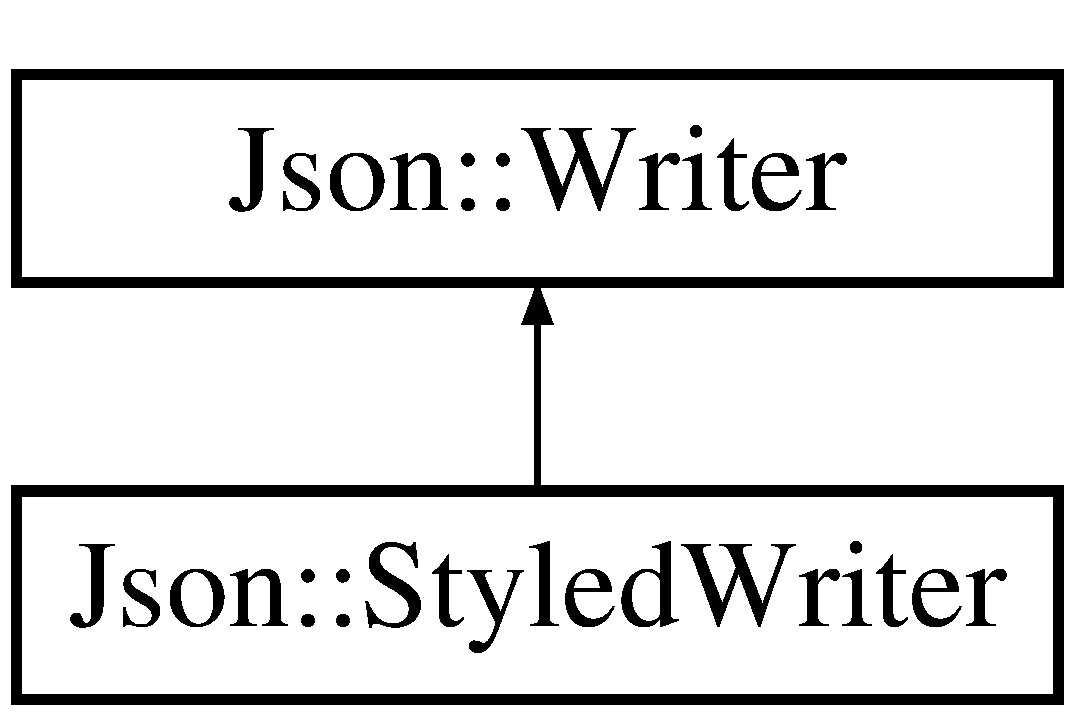
\includegraphics[height=2.000000cm]{class_json_1_1_styled_writer}
\end{center}
\end{figure}
\subsection*{Public Member Functions}
\begin{DoxyCompactItemize}
\item 
virtual std\-::string \hyperlink{class_json_1_1_styled_writer_a56f0fd80f60272b3f3c85690aae66e7d}{write} (const \hyperlink{class_json_1_1_value}{Value} \&root)
\begin{DoxyCompactList}\small\item\em Serialize a \hyperlink{class_json_1_1_value}{Value} in \href{http://www.json.org}{\tt J\-S\-O\-N} format. \end{DoxyCompactList}\end{DoxyCompactItemize}


\subsection{Detailed Description}
Writes a \hyperlink{class_json_1_1_value}{Value} in \href{http://www.json.org}{\tt J\-S\-O\-N} format in a human friendly way. 

The rules for line break and indent are as follow\-:
\begin{DoxyItemize}
\item Object value\-:
\begin{DoxyItemize}
\item if empty then print \{\} without indent and line break
\item if not empty the print '\{', line break \& indent, print one value per line and then unindent and line break and print '\}'.
\end{DoxyItemize}
\item Array value\-:
\begin{DoxyItemize}
\item if empty then print \mbox{[}\mbox{]} without indent and line break
\item if the array contains no object value, empty array or some other value types, and all the values fit on one lines, then print the array on a single line.
\item otherwise, it the values do not fit on one line, or the array contains object or non empty array, then print one value per line.
\end{DoxyItemize}
\end{DoxyItemize}

If the \hyperlink{class_json_1_1_value}{Value} have comments then they are outputed according to their \hyperlink{namespace_json_a4fc417c23905b2ae9e2c47d197a45351}{Comment\-Placement}.

\begin{DoxySeeAlso}{See Also}
\hyperlink{class_json_1_1_reader}{Reader}, \hyperlink{class_json_1_1_value}{Value}, \hyperlink{class_json_1_1_value_a29f3a30f7e5d3af6f38d57999bf5b480}{Value\-::set\-Comment()} 
\end{DoxySeeAlso}


\subsection{Member Function Documentation}
\hypertarget{class_json_1_1_styled_writer_a56f0fd80f60272b3f3c85690aae66e7d}{\index{Json\-::\-Styled\-Writer@{Json\-::\-Styled\-Writer}!write@{write}}
\index{write@{write}!Json::StyledWriter@{Json\-::\-Styled\-Writer}}
\subsubsection[{write}]{\setlength{\rightskip}{0pt plus 5cm}std\-::string Json\-::\-Styled\-Writer\-::write (
\begin{DoxyParamCaption}
\item[{const {\bf Value} \&}]{root}
\end{DoxyParamCaption}
)\hspace{0.3cm}{\ttfamily [virtual]}}}\label{class_json_1_1_styled_writer_a56f0fd80f60272b3f3c85690aae66e7d}


Serialize a \hyperlink{class_json_1_1_value}{Value} in \href{http://www.json.org}{\tt J\-S\-O\-N} format. 


\begin{DoxyParams}{Parameters}
{\em root} & \hyperlink{class_json_1_1_value}{Value} to serialize. \\
\hline
\end{DoxyParams}
\begin{DoxyReturn}{Returns}
String containing the J\-S\-O\-N document that represents the root value. 
\end{DoxyReturn}


Implements \hyperlink{class_json_1_1_writer}{Json\-::\-Writer}.



The documentation for this class was generated from the following files\-:\begin{DoxyCompactItemize}
\item 
include/json/json.\-h\item 
src/jsoncpp.\-cpp\end{DoxyCompactItemize}

\hypertarget{struct_sub_program}{\section{Sub\-Program Struct Reference}
\label{struct_sub_program}\index{Sub\-Program@{Sub\-Program}}
}
\subsection*{Public Attributes}
\begin{DoxyCompactItemize}
\item 
\hypertarget{struct_sub_program_aa9bb1992fed633d182076a35d6448c7d}{\hyperlink{struct_vdbe_op}{Vdbe\-Op} $\ast$ {\bfseries a\-Op}}\label{struct_sub_program_aa9bb1992fed633d182076a35d6448c7d}

\item 
\hypertarget{struct_sub_program_a6fe204a75ab8254c453be77f024b6d69}{int {\bfseries n\-Op}}\label{struct_sub_program_a6fe204a75ab8254c453be77f024b6d69}

\item 
\hypertarget{struct_sub_program_a9bece42fdeb81085809d7c2f8aa05616}{int {\bfseries n\-Mem}}\label{struct_sub_program_a9bece42fdeb81085809d7c2f8aa05616}

\item 
\hypertarget{struct_sub_program_a83b18aa5cc63aecdbf996c16af1e48bb}{int {\bfseries n\-Csr}}\label{struct_sub_program_a83b18aa5cc63aecdbf996c16af1e48bb}

\item 
\hypertarget{struct_sub_program_a907d5933dd0149be1ef90fcbe91e3c58}{int {\bfseries n\-Once}}\label{struct_sub_program_a907d5933dd0149be1ef90fcbe91e3c58}

\item 
\hypertarget{struct_sub_program_aaea3b67899b092476b107d22a4e2022d}{void $\ast$ {\bfseries token}}\label{struct_sub_program_aaea3b67899b092476b107d22a4e2022d}

\item 
\hypertarget{struct_sub_program_a7da35488ac58a64fa30b88da56aac8b3}{\hyperlink{struct_sub_program}{Sub\-Program} $\ast$ {\bfseries p\-Next}}\label{struct_sub_program_a7da35488ac58a64fa30b88da56aac8b3}

\end{DoxyCompactItemize}


The documentation for this struct was generated from the following file\-:\begin{DoxyCompactItemize}
\item 
src/sqlite3.\-c\end{DoxyCompactItemize}

\hypertarget{struct_sum_ctx}{\section{Sum\-Ctx Struct Reference}
\label{struct_sum_ctx}\index{Sum\-Ctx@{Sum\-Ctx}}
}
\subsection*{Public Attributes}
\begin{DoxyCompactItemize}
\item 
\hypertarget{struct_sum_ctx_a1774080b9bcada2f4e867eaf40763f41}{double {\bfseries r\-Sum}}\label{struct_sum_ctx_a1774080b9bcada2f4e867eaf40763f41}

\item 
\hypertarget{struct_sum_ctx_ace6196fb30ebc0687997a723d55683db}{i64 {\bfseries i\-Sum}}\label{struct_sum_ctx_ace6196fb30ebc0687997a723d55683db}

\item 
\hypertarget{struct_sum_ctx_ada00261fe604a7cc6719fdcd8bb5914c}{i64 {\bfseries cnt}}\label{struct_sum_ctx_ada00261fe604a7cc6719fdcd8bb5914c}

\item 
\hypertarget{struct_sum_ctx_a3b14a5da00584aff08314d5e9ddbe9ea}{u8 {\bfseries overflow}}\label{struct_sum_ctx_a3b14a5da00584aff08314d5e9ddbe9ea}

\item 
\hypertarget{struct_sum_ctx_a035a2a22271fee066d9a92d12fe3b9a5}{u8 {\bfseries approx}}\label{struct_sum_ctx_a035a2a22271fee066d9a92d12fe3b9a5}

\end{DoxyCompactItemize}


The documentation for this struct was generated from the following file\-:\begin{DoxyCompactItemize}
\item 
src/sqlite3.\-c\end{DoxyCompactItemize}

\hypertarget{struct_table}{\section{Table Struct Reference}
\label{struct_table}\index{Table@{Table}}
}
\subsection*{Public Attributes}
\begin{DoxyCompactItemize}
\item 
\hypertarget{struct_table_a20ca62607d6da596b1016b76cf677809}{char $\ast$ {\bfseries z\-Name}}\label{struct_table_a20ca62607d6da596b1016b76cf677809}

\item 
\hypertarget{struct_table_a87ec3b706ecf9545bd9ed582a12ce3e7}{\hyperlink{struct_column}{Column} $\ast$ {\bfseries a\-Col}}\label{struct_table_a87ec3b706ecf9545bd9ed582a12ce3e7}

\item 
\hypertarget{struct_table_a5dffd0c9e8f0265d6a47b32bd0e6d59f}{\hyperlink{struct_index}{Index} $\ast$ {\bfseries p\-Index}}\label{struct_table_a5dffd0c9e8f0265d6a47b32bd0e6d59f}

\item 
\hypertarget{struct_table_a39d620182fe2174fc97d04094421fa60}{\hyperlink{struct_select}{Select} $\ast$ {\bfseries p\-Select}}\label{struct_table_a39d620182fe2174fc97d04094421fa60}

\item 
\hypertarget{struct_table_a37ccce5ee6d530001d49c82788c6616d}{\hyperlink{struct_f_key}{F\-Key} $\ast$ {\bfseries p\-F\-Key}}\label{struct_table_a37ccce5ee6d530001d49c82788c6616d}

\item 
\hypertarget{struct_table_ac95c0c7b04f2c8367beb98d386d4228f}{char $\ast$ {\bfseries z\-Col\-Aff}}\label{struct_table_ac95c0c7b04f2c8367beb98d386d4228f}

\item 
\hypertarget{struct_table_a4513ad39c4adad36fdf5dd3c6cb70a12}{\hyperlink{struct_expr_list}{Expr\-List} $\ast$ {\bfseries p\-Check}}\label{struct_table_a4513ad39c4adad36fdf5dd3c6cb70a12}

\item 
\hypertarget{struct_table_a909f316fb8c4f86771ae1b5e55c23230}{t\-Rowcnt {\bfseries n\-Row\-Est}}\label{struct_table_a909f316fb8c4f86771ae1b5e55c23230}

\item 
\hypertarget{struct_table_aebe1abbfb2fd4b5e5dff8e74a4f3c890}{int {\bfseries tnum}}\label{struct_table_aebe1abbfb2fd4b5e5dff8e74a4f3c890}

\item 
\hypertarget{struct_table_af5e592498393a990cb1344555fa86409}{i16 {\bfseries i\-P\-Key}}\label{struct_table_af5e592498393a990cb1344555fa86409}

\item 
\hypertarget{struct_table_a1a8346811ba23fdfd90c5b54076bbefb}{i16 {\bfseries n\-Col}}\label{struct_table_a1a8346811ba23fdfd90c5b54076bbefb}

\item 
\hypertarget{struct_table_a5c3d59f52186917d412d42e008dd302c}{u16 {\bfseries n\-Ref}}\label{struct_table_a5c3d59f52186917d412d42e008dd302c}

\item 
\hypertarget{struct_table_ab0aeb112ae7e1b81e2a18bc493f7992c}{u8 {\bfseries tab\-Flags}}\label{struct_table_ab0aeb112ae7e1b81e2a18bc493f7992c}

\item 
\hypertarget{struct_table_add1b22425db781d976d25b4465a2965a}{u8 {\bfseries key\-Conf}}\label{struct_table_add1b22425db781d976d25b4465a2965a}

\item 
\hypertarget{struct_table_ab6f1ad10bce5c20faca55cd0a9c3f1ff}{int {\bfseries add\-Col\-Offset}}\label{struct_table_ab6f1ad10bce5c20faca55cd0a9c3f1ff}

\item 
\hypertarget{struct_table_a74a2c5547ea876ebe77dbea0d99361bf}{int {\bfseries n\-Module\-Arg}}\label{struct_table_a74a2c5547ea876ebe77dbea0d99361bf}

\item 
\hypertarget{struct_table_af3af6596efa41894bcd3c3c9f9b6781f}{char $\ast$$\ast$ {\bfseries az\-Module\-Arg}}\label{struct_table_af3af6596efa41894bcd3c3c9f9b6781f}

\item 
\hypertarget{struct_table_a7b9903cfbfefe7b8bf872c4f50cb2e95}{\hyperlink{struct_v_table}{V\-Table} $\ast$ {\bfseries p\-V\-Table}}\label{struct_table_a7b9903cfbfefe7b8bf872c4f50cb2e95}

\item 
\hypertarget{struct_table_aca61c40bb0164f2c6fc3406c28988660}{\hyperlink{struct_trigger}{Trigger} $\ast$ {\bfseries p\-Trigger}}\label{struct_table_aca61c40bb0164f2c6fc3406c28988660}

\item 
\hypertarget{struct_table_a1d6ce038a061722cebaeba0f3ffceacf}{\hyperlink{struct_schema}{Schema} $\ast$ {\bfseries p\-Schema}}\label{struct_table_a1d6ce038a061722cebaeba0f3ffceacf}

\item 
\hypertarget{struct_table_ae365eb0d8f6d3cb39f3908323cba45e4}{\hyperlink{struct_table}{Table} $\ast$ {\bfseries p\-Next\-Zombie}}\label{struct_table_ae365eb0d8f6d3cb39f3908323cba45e4}

\end{DoxyCompactItemize}


The documentation for this struct was generated from the following file\-:\begin{DoxyCompactItemize}
\item 
src/sqlite3.\-c\end{DoxyCompactItemize}

\hypertarget{struct_table_lock}{\section{Table\-Lock Struct Reference}
\label{struct_table_lock}\index{Table\-Lock@{Table\-Lock}}
}
\subsection*{Public Attributes}
\begin{DoxyCompactItemize}
\item 
\hypertarget{struct_table_lock_ad5cc726ef29ffcca39ec0b72942513f6}{int {\bfseries i\-Db}}\label{struct_table_lock_ad5cc726ef29ffcca39ec0b72942513f6}

\item 
\hypertarget{struct_table_lock_ab25b5d9ba21ed96ed68ce8064ff84e24}{int {\bfseries i\-Tab}}\label{struct_table_lock_ab25b5d9ba21ed96ed68ce8064ff84e24}

\item 
\hypertarget{struct_table_lock_a171121af9886ee08044d4b82b991ceeb}{u8 {\bfseries is\-Write\-Lock}}\label{struct_table_lock_a171121af9886ee08044d4b82b991ceeb}

\item 
\hypertarget{struct_table_lock_ad1ce077fbd2600dd6d23ec08706dd227}{const char $\ast$ {\bfseries z\-Name}}\label{struct_table_lock_ad1ce077fbd2600dd6d23ec08706dd227}

\end{DoxyCompactItemize}


The documentation for this struct was generated from the following file\-:\begin{DoxyCompactItemize}
\item 
src/sqlite3.\-c\end{DoxyCompactItemize}

\hypertarget{struct_tab_result}{\section{Tab\-Result Struct Reference}
\label{struct_tab_result}\index{Tab\-Result@{Tab\-Result}}
}
\subsection*{Public Attributes}
\begin{DoxyCompactItemize}
\item 
\hypertarget{struct_tab_result_a7446a22a7b39c17e447c65ba200490a6}{char $\ast$$\ast$ {\bfseries az\-Result}}\label{struct_tab_result_a7446a22a7b39c17e447c65ba200490a6}

\item 
\hypertarget{struct_tab_result_a6e7104bb622be05f16b6470dbb68a6c7}{char $\ast$ {\bfseries z\-Err\-Msg}}\label{struct_tab_result_a6e7104bb622be05f16b6470dbb68a6c7}

\item 
\hypertarget{struct_tab_result_a6a1d5bc64a1eeef54b56cb2602b663b2}{int {\bfseries n\-Alloc}}\label{struct_tab_result_a6a1d5bc64a1eeef54b56cb2602b663b2}

\item 
\hypertarget{struct_tab_result_ae803d6f07364c9e03bee8abd13056e1b}{int {\bfseries n\-Row}}\label{struct_tab_result_ae803d6f07364c9e03bee8abd13056e1b}

\item 
\hypertarget{struct_tab_result_a44237b9ab33cdbca7a5a158470ebcaa3}{int {\bfseries n\-Column}}\label{struct_tab_result_a44237b9ab33cdbca7a5a158470ebcaa3}

\item 
\hypertarget{struct_tab_result_a959e8dd3348f76e4cdabad9c89ee62d1}{int {\bfseries n\-Data}}\label{struct_tab_result_a959e8dd3348f76e4cdabad9c89ee62d1}

\item 
\hypertarget{struct_tab_result_a44bb015ce660ed3f987e324919d73f4d}{int {\bfseries rc}}\label{struct_tab_result_a44bb015ce660ed3f987e324919d73f4d}

\end{DoxyCompactItemize}


The documentation for this struct was generated from the following file\-:\begin{DoxyCompactItemize}
\item 
src/sqlite3.\-c\end{DoxyCompactItemize}

\hypertarget{class_target_block}{\section{Target\-Block Class Reference}
\label{class_target_block}\index{Target\-Block@{Target\-Block}}
}
Inheritance diagram for Target\-Block\-:\begin{figure}[H]
\begin{center}
\leavevmode
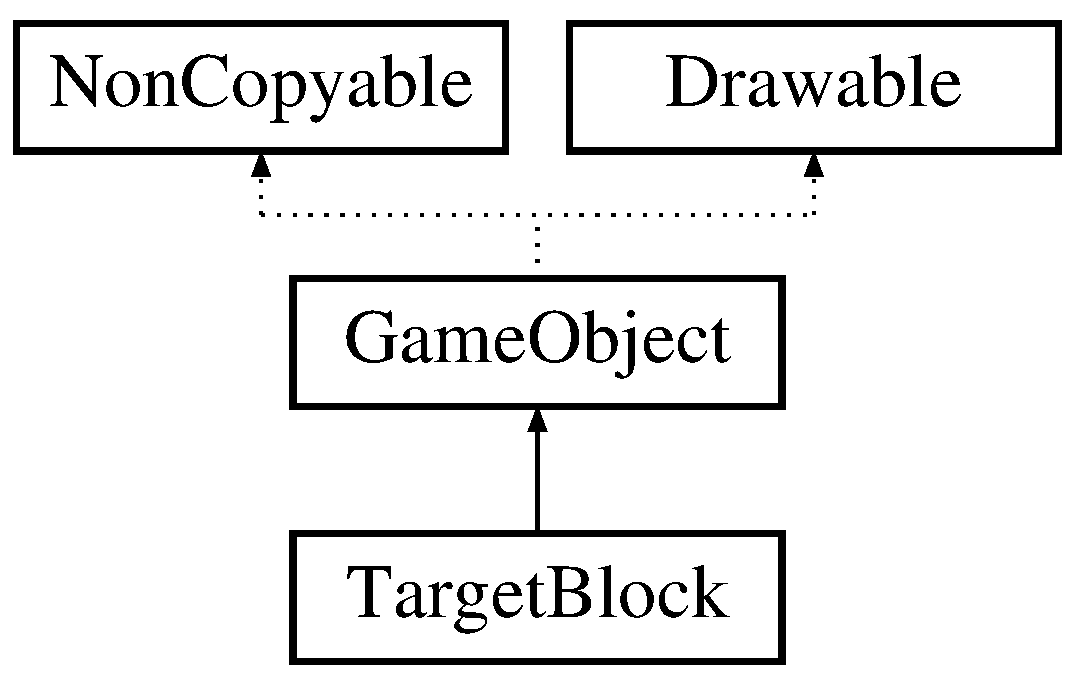
\includegraphics[height=3.000000cm]{class_target_block}
\end{center}
\end{figure}
\subsection*{Public Member Functions}
\begin{DoxyCompactItemize}
\item 
\hypertarget{class_target_block_a0d862260d9ea6052a28b87b2d93abb4d}{{\bfseries Target\-Block} (const std\-::string \&name, const sf\-::\-Texture \&t)}\label{class_target_block_a0d862260d9ea6052a28b87b2d93abb4d}

\end{DoxyCompactItemize}
\subsection*{Protected Member Functions}
\begin{DoxyCompactItemize}
\item 
\hypertarget{class_target_block_a872f6dd250b9e0904dfd90bad8bdf42a}{virtual void {\bfseries draw} (sf\-::\-Render\-Target \&target, sf\-::\-Render\-States states) const }\label{class_target_block_a872f6dd250b9e0904dfd90bad8bdf42a}

\item 
\hypertarget{class_target_block_a2c16d7dd07e04c085bbd5a7cc1151437}{virtual void {\bfseries update} ()}\label{class_target_block_a2c16d7dd07e04c085bbd5a7cc1151437}

\end{DoxyCompactItemize}
\subsection*{Additional Inherited Members}


The documentation for this class was generated from the following files\-:\begin{DoxyCompactItemize}
\item 
include/Target\-Block.\-hpp\item 
src/Target\-Block.\-cpp\end{DoxyCompactItemize}

\hypertarget{class_target_list}{\section{Target\-List Class Reference}
\label{class_target_list}\index{Target\-List@{Target\-List}}
}


Send list of targets in one go.  




{\ttfamily \#include $<$Network\-Events.\-h$>$}

Inheritance diagram for Target\-List\-:\begin{figure}[H]
\begin{center}
\leavevmode
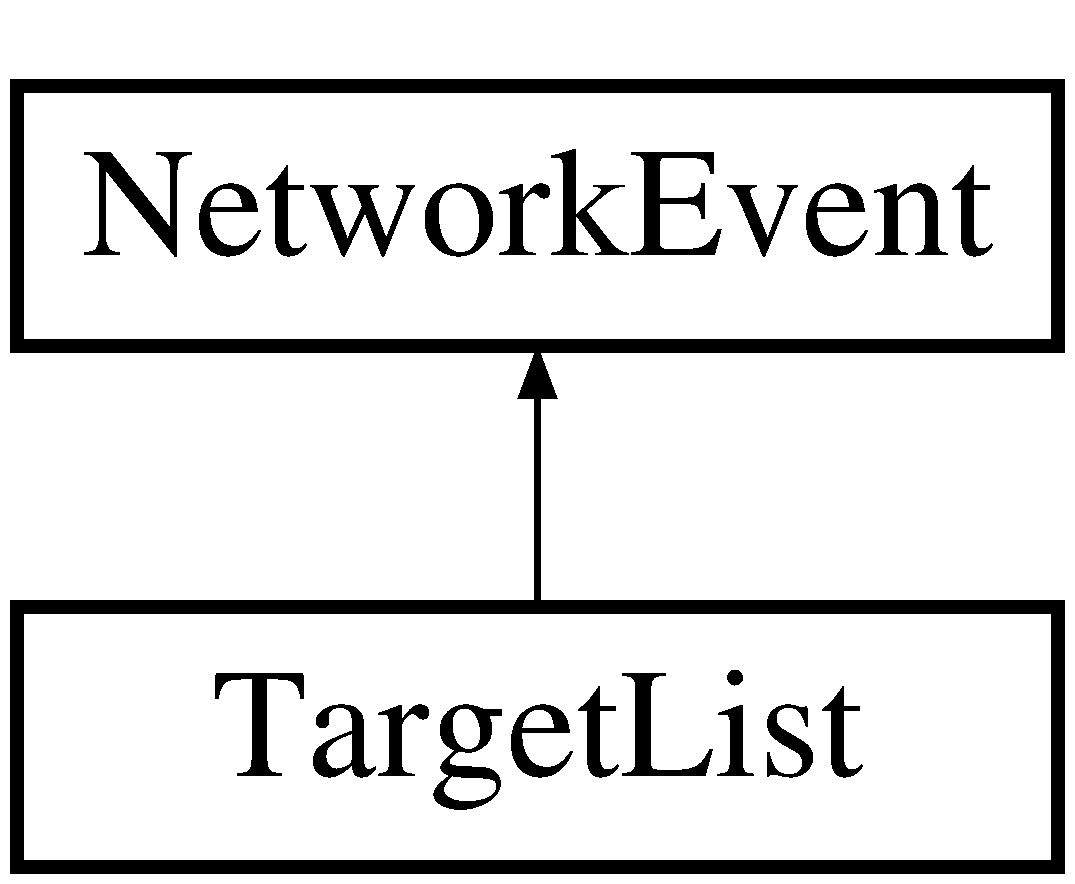
\includegraphics[height=2.000000cm]{class_target_list}
\end{center}
\end{figure}
\subsection*{Public Member Functions}
\begin{DoxyCompactItemize}
\item 
\hypertarget{class_target_list_a645770f4c609ff6cf83ebed701ef6644}{virtual sf\-::\-Int32 {\bfseries get\-Command} () const }\label{class_target_list_a645770f4c609ff6cf83ebed701ef6644}

\end{DoxyCompactItemize}
\subsection*{Public Attributes}
\begin{DoxyCompactItemize}
\item 
\hypertarget{class_target_list_a5ca9ed23341ce1483d5fb77724ca68a1}{unsigned int {\bfseries entry\-Count}}\label{class_target_list_a5ca9ed23341ce1483d5fb77724ca68a1}

\item 
\hypertarget{class_target_list_a7e1571e9657d022ecac52125d631b911}{std\-::vector$<$ unsigned int $>$ {\bfseries target\-Ids}}\label{class_target_list_a7e1571e9657d022ecac52125d631b911}

\item 
\hypertarget{class_target_list_a24fb83f4fa75f5444353f33341300956}{std\-::vector$<$ glm\-::vec2 $>$ {\bfseries target\-Positions}}\label{class_target_list_a24fb83f4fa75f5444353f33341300956}

\end{DoxyCompactItemize}
\subsection*{Friends}
\begin{DoxyCompactItemize}
\item 
\hypertarget{class_target_list_a5e3531afd8ddbd5fa0a17a28ac892522}{sf\-::\-Packet \& {\bfseries operator$<$$<$} (sf\-::\-Packet \&packet, const \hyperlink{class_target_list}{Target\-List} \&targets)}\label{class_target_list_a5e3531afd8ddbd5fa0a17a28ac892522}

\item 
\hypertarget{class_target_list_ab08d74760edd840b452538362d85259f}{sf\-::\-Packet \& {\bfseries operator$>$$>$} (sf\-::\-Packet \&packet, \hyperlink{class_target_list}{Target\-List} \&targets)}\label{class_target_list_ab08d74760edd840b452538362d85259f}

\end{DoxyCompactItemize}
\subsection*{Additional Inherited Members}


\subsection{Detailed Description}
Send list of targets in one go. 



The documentation for this class was generated from the following file\-:\begin{DoxyCompactItemize}
\item 
include/Network\-Events.\-h\end{DoxyCompactItemize}

\hypertarget{class_text_input_field}{\section{Text\-Input\-Field Class Reference}
\label{class_text_input_field}\index{Text\-Input\-Field@{Text\-Input\-Field}}
}
Inheritance diagram for Text\-Input\-Field\-:\begin{figure}[H]
\begin{center}
\leavevmode
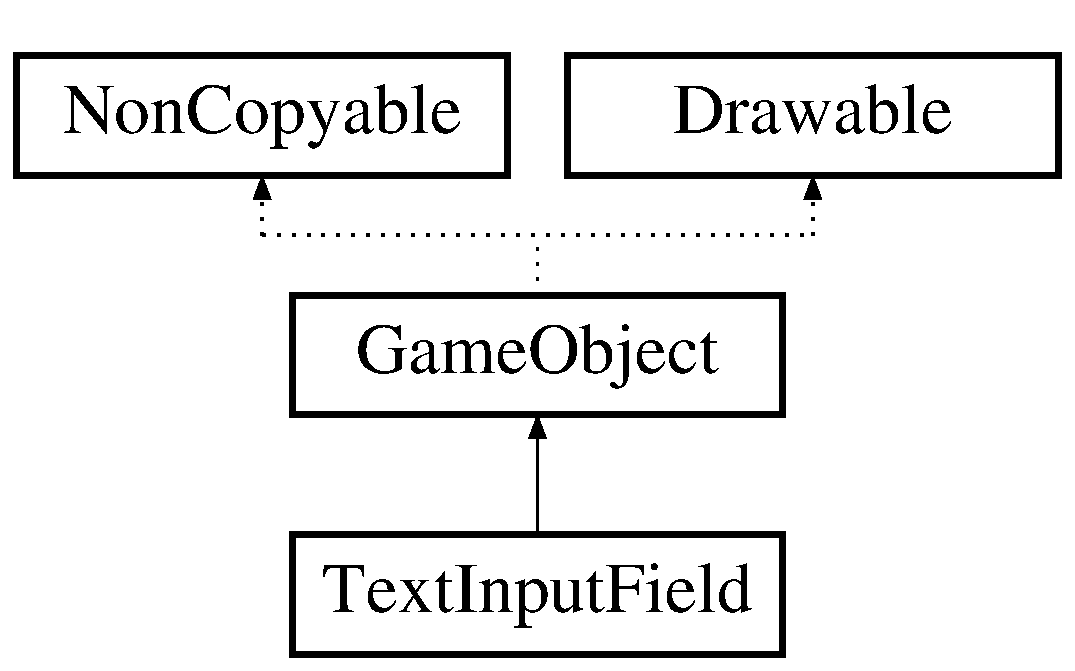
\includegraphics[height=3.000000cm]{class_text_input_field}
\end{center}
\end{figure}
\subsection*{Public Member Functions}
\begin{DoxyCompactItemize}
\item 
\hypertarget{class_text_input_field_a3f41714f69478545a3756c0000f7e56e}{{\bfseries Text\-Input\-Field} (const std\-::string \&name, const sf\-::\-Vector2f \&position, const sf\-::\-Vector2f \&size)}\label{class_text_input_field_a3f41714f69478545a3756c0000f7e56e}

\item 
\hypertarget{class_text_input_field_a67cf6582f3279aef7cc16d329ab2bbfc}{void {\bfseries open} ()}\label{class_text_input_field_a67cf6582f3279aef7cc16d329ab2bbfc}

\item 
\hypertarget{class_text_input_field_a345495b23609fb42746bdfc873ad425c}{void {\bfseries close} ()}\label{class_text_input_field_a345495b23609fb42746bdfc873ad425c}

\item 
\hypertarget{class_text_input_field_a34eb88372fb6dd4e0f84b47fd6170318}{void {\bfseries set\-Label\-Text} (const std\-::string \&label\-Text)}\label{class_text_input_field_a34eb88372fb6dd4e0f84b47fd6170318}

\item 
\hypertarget{class_text_input_field_ac4c2e650b8481662eaf87b4d0a0e2e68}{const std\-::string \& {\bfseries get\-Input} () const }\label{class_text_input_field_ac4c2e650b8481662eaf87b4d0a0e2e68}

\item 
\hypertarget{class_text_input_field_a7e54c81f77d20cf1e7a1a5580b2d6827}{bool {\bfseries get\-Open} () const }\label{class_text_input_field_a7e54c81f77d20cf1e7a1a5580b2d6827}

\item 
\hypertarget{class_text_input_field_a831cacc7a0e0191a354b24c7e9ca6186}{bool {\bfseries is\-Ready} () const }\label{class_text_input_field_a831cacc7a0e0191a354b24c7e9ca6186}

\item 
\hypertarget{class_text_input_field_acae36fdc758a9c783ebe329e650b697e}{void {\bfseries update} ()}\label{class_text_input_field_acae36fdc758a9c783ebe329e650b697e}

\item 
\hypertarget{class_text_input_field_a5469a141665b1cc321b6d59b8d4de7fd}{void {\bfseries set\-Allowed\-Letters} (const std\-::string \&str)}\label{class_text_input_field_a5469a141665b1cc321b6d59b8d4de7fd}

\item 
\hypertarget{class_text_input_field_a844c6ce12cb179bb2dd55a3491be0ef4}{void {\bfseries set\-Text} (const std\-::string \&txt)}\label{class_text_input_field_a844c6ce12cb179bb2dd55a3491be0ef4}

\end{DoxyCompactItemize}
\subsection*{Protected Member Functions}
\begin{DoxyCompactItemize}
\item 
\hypertarget{class_text_input_field_a6d6e2b1cfde181724d1039c0991a7483}{virtual void {\bfseries draw} (sf\-::\-Render\-Target \&target, sf\-::\-Render\-States states=sf\-::\-Render\-States\-::\-Default) const }\label{class_text_input_field_a6d6e2b1cfde181724d1039c0991a7483}

\end{DoxyCompactItemize}
\subsection*{Additional Inherited Members}


The documentation for this class was generated from the following files\-:\begin{DoxyCompactItemize}
\item 
include/Text\-Input\-Field.\-hpp\item 
src/Text\-Input\-Field.\-cpp\end{DoxyCompactItemize}

\hypertarget{class_time}{\section{Time Class Reference}
\label{class_time}\index{Time@{Time}}
}
\subsection*{Static Public Attributes}
\begin{DoxyCompactItemize}
\item 
\hypertarget{class_time_a35fe30294c847679da506b540f05d593}{static float {\bfseries delta\-Time}}\label{class_time_a35fe30294c847679da506b540f05d593}

\item 
\hypertarget{class_time_ace6e056882b2b2f73b1f8870c8c0dccb}{static float {\bfseries time}}\label{class_time_ace6e056882b2b2f73b1f8870c8c0dccb}

\end{DoxyCompactItemize}
\subsection*{Friends}
\begin{DoxyCompactItemize}
\item 
\hypertarget{class_time_aa2fab026580d6f14280c2ffb8063a314}{class {\bfseries Game}}\label{class_time_aa2fab026580d6f14280c2ffb8063a314}

\item 
\hypertarget{class_time_ac2055578ac48afabe5af487878450f68}{class {\bfseries Server}}\label{class_time_ac2055578ac48afabe5af487878450f68}

\end{DoxyCompactItemize}


The documentation for this class was generated from the following files\-:\begin{DoxyCompactItemize}
\item 
include/Time.\-hpp\item 
src/Time.\-cpp\end{DoxyCompactItemize}

\hypertarget{struct_token}{\section{Token Struct Reference}
\label{struct_token}\index{Token@{Token}}
}
\subsection*{Public Attributes}
\begin{DoxyCompactItemize}
\item 
\hypertarget{struct_token_a57b502141e3018e4a02773424acb4ffd}{const char $\ast$ {\bfseries z}}\label{struct_token_a57b502141e3018e4a02773424acb4ffd}

\item 
\hypertarget{struct_token_ad8442439e00ab9713a9b91a53e44c2aa}{unsigned int {\bfseries n}}\label{struct_token_ad8442439e00ab9713a9b91a53e44c2aa}

\end{DoxyCompactItemize}


The documentation for this struct was generated from the following file\-:\begin{DoxyCompactItemize}
\item 
src/sqlite3.\-c\end{DoxyCompactItemize}

\hypertarget{class_transform}{\section{Transform Class Reference}
\label{class_transform}\index{Transform@{Transform}}
}
\subsection*{Public Types}
\begin{DoxyCompactItemize}
\item 
\hypertarget{class_transform_a58b9808d3d9a4f1a04f2ed7ee5cff0f0}{typedef std\-::vector$<$ \hyperlink{class_transform}{Transform} $\ast$ $>$ {\bfseries Children}}\label{class_transform_a58b9808d3d9a4f1a04f2ed7ee5cff0f0}

\end{DoxyCompactItemize}
\subsection*{Public Member Functions}
\begin{DoxyCompactItemize}
\item 
\hypertarget{class_transform_ab331def81fa1a08e1f14b0ae977a98cb}{glm\-::vec2 {\bfseries get\-Local\-Position} () const }\label{class_transform_ab331def81fa1a08e1f14b0ae977a98cb}

\item 
\hypertarget{class_transform_a2d4f4b7192cca6765638ef29a0519935}{sf\-::\-Vector2f {\bfseries get\-Position\-Sf} () const }\label{class_transform_a2d4f4b7192cca6765638ef29a0519935}

\item 
\hypertarget{class_transform_a5da75c53ee14bcc1042a192df5f3f0b7}{void {\bfseries set\-Local\-Position} (const glm\-::vec2 \&new\-Pos)}\label{class_transform_a5da75c53ee14bcc1042a192df5f3f0b7}

\item 
\hypertarget{class_transform_a0bbb28cce7bca9363703b41ca10dcc57}{void {\bfseries set\-Parent} (\hyperlink{class_transform}{Transform} $\ast$par)}\label{class_transform_a0bbb28cce7bca9363703b41ca10dcc57}

\item 
\hypertarget{class_transform_a32f297083089e707628cd01dac598e40}{\hyperlink{class_transform}{Transform} \& {\bfseries get\-Parent} () const }\label{class_transform_a32f297083089e707628cd01dac598e40}

\item 
\hypertarget{class_transform_a6d76a64ce6feb3c8f3eb45352b77f74c}{Children \& {\bfseries get\-Children} ()}\label{class_transform_a6d76a64ce6feb3c8f3eb45352b77f74c}

\end{DoxyCompactItemize}
\subsection*{Public Attributes}
\begin{DoxyCompactItemize}
\item 
\hypertarget{class_transform_afea9a04d0ed015813204e8b2d4c40666}{\hyperlink{class_game_object}{Game\-Object} \& {\bfseries game\-Object}}\label{class_transform_afea9a04d0ed015813204e8b2d4c40666}

\end{DoxyCompactItemize}
\subsection*{Friends}
\begin{DoxyCompactItemize}
\item 
\hypertarget{class_transform_a00df87c957d8f7ee0fc51f07a0542f4a}{class {\bfseries Game\-Object}}\label{class_transform_a00df87c957d8f7ee0fc51f07a0542f4a}

\end{DoxyCompactItemize}


The documentation for this class was generated from the following files\-:\begin{DoxyCompactItemize}
\item 
include/Transform.\-hpp\item 
src/Transform.\-cpp\end{DoxyCompactItemize}

\hypertarget{struct_trig_event}{\section{Trig\-Event Struct Reference}
\label{struct_trig_event}\index{Trig\-Event@{Trig\-Event}}
}
\subsection*{Public Attributes}
\begin{DoxyCompactItemize}
\item 
\hypertarget{struct_trig_event_a19ac5a5e59e08350f72ec49cf8fccbb6}{int {\bfseries a}}\label{struct_trig_event_a19ac5a5e59e08350f72ec49cf8fccbb6}

\item 
\hypertarget{struct_trig_event_a86ef160cde95382e98b7934614e7f79f}{\hyperlink{struct_id_list}{Id\-List} $\ast$ {\bfseries b}}\label{struct_trig_event_a86ef160cde95382e98b7934614e7f79f}

\end{DoxyCompactItemize}


The documentation for this struct was generated from the following file\-:\begin{DoxyCompactItemize}
\item 
src/sqlite3.\-c\end{DoxyCompactItemize}

\hypertarget{struct_trigger}{\section{Trigger Struct Reference}
\label{struct_trigger}\index{Trigger@{Trigger}}
}
\subsection*{Public Attributes}
\begin{DoxyCompactItemize}
\item 
\hypertarget{struct_trigger_a9aecea5dadd7ae93b7f585c4b914791c}{char $\ast$ {\bfseries z\-Name}}\label{struct_trigger_a9aecea5dadd7ae93b7f585c4b914791c}

\item 
\hypertarget{struct_trigger_ab9d5500f7fc43382e867733a2968ecae}{char $\ast$ {\bfseries table}}\label{struct_trigger_ab9d5500f7fc43382e867733a2968ecae}

\item 
\hypertarget{struct_trigger_a855d6b6a302d8d80e1d30ddd70fd403e}{u8 {\bfseries op}}\label{struct_trigger_a855d6b6a302d8d80e1d30ddd70fd403e}

\item 
\hypertarget{struct_trigger_af0d10da140b068bfd76aaeb6607fa6cf}{u8 {\bfseries tr\-\_\-tm}}\label{struct_trigger_af0d10da140b068bfd76aaeb6607fa6cf}

\item 
\hypertarget{struct_trigger_a1b6cdd46e8b98562920d1acee86281ed}{\hyperlink{struct_expr}{Expr} $\ast$ {\bfseries p\-When}}\label{struct_trigger_a1b6cdd46e8b98562920d1acee86281ed}

\item 
\hypertarget{struct_trigger_a8505fbdf63ca9eadf4b2585e99faa4e4}{\hyperlink{struct_id_list}{Id\-List} $\ast$ {\bfseries p\-Columns}}\label{struct_trigger_a8505fbdf63ca9eadf4b2585e99faa4e4}

\item 
\hypertarget{struct_trigger_a83edbfa91ce6520a6ebc1a21acc2cd5e}{\hyperlink{struct_schema}{Schema} $\ast$ {\bfseries p\-Schema}}\label{struct_trigger_a83edbfa91ce6520a6ebc1a21acc2cd5e}

\item 
\hypertarget{struct_trigger_a8e4a9b3f4bcc5c645e1777b3bb94a6d8}{\hyperlink{struct_schema}{Schema} $\ast$ {\bfseries p\-Tab\-Schema}}\label{struct_trigger_a8e4a9b3f4bcc5c645e1777b3bb94a6d8}

\item 
\hypertarget{struct_trigger_a4206faaae6cdf1a2b22a2c9f15c88642}{\hyperlink{struct_trigger_step}{Trigger\-Step} $\ast$ {\bfseries step\-\_\-list}}\label{struct_trigger_a4206faaae6cdf1a2b22a2c9f15c88642}

\item 
\hypertarget{struct_trigger_ac28107e1c45789e0146fe45867b8dfdb}{\hyperlink{struct_trigger}{Trigger} $\ast$ {\bfseries p\-Next}}\label{struct_trigger_ac28107e1c45789e0146fe45867b8dfdb}

\end{DoxyCompactItemize}


The documentation for this struct was generated from the following file\-:\begin{DoxyCompactItemize}
\item 
src/sqlite3.\-c\end{DoxyCompactItemize}

\hypertarget{struct_trigger_prg}{\section{Trigger\-Prg Struct Reference}
\label{struct_trigger_prg}\index{Trigger\-Prg@{Trigger\-Prg}}
}
\subsection*{Public Attributes}
\begin{DoxyCompactItemize}
\item 
\hypertarget{struct_trigger_prg_af70e5a74c954bc7a1eb8ee1162c40368}{\hyperlink{struct_trigger}{Trigger} $\ast$ {\bfseries p\-Trigger}}\label{struct_trigger_prg_af70e5a74c954bc7a1eb8ee1162c40368}

\item 
\hypertarget{struct_trigger_prg_a551b8a29a8c4ff785afab1596e5d8710}{\hyperlink{struct_trigger_prg}{Trigger\-Prg} $\ast$ {\bfseries p\-Next}}\label{struct_trigger_prg_a551b8a29a8c4ff785afab1596e5d8710}

\item 
\hypertarget{struct_trigger_prg_aa770aee270c7c5df85578dc4a6686134}{\hyperlink{struct_sub_program}{Sub\-Program} $\ast$ {\bfseries p\-Program}}\label{struct_trigger_prg_aa770aee270c7c5df85578dc4a6686134}

\item 
\hypertarget{struct_trigger_prg_aa475acda58c472b3491f6aa17020bf68}{int {\bfseries orconf}}\label{struct_trigger_prg_aa475acda58c472b3491f6aa17020bf68}

\item 
\hypertarget{struct_trigger_prg_aeac0a4cd1f1d287981ae33c4d171b614}{u32 {\bfseries a\-Colmask} \mbox{[}2\mbox{]}}\label{struct_trigger_prg_aeac0a4cd1f1d287981ae33c4d171b614}

\end{DoxyCompactItemize}


The documentation for this struct was generated from the following file\-:\begin{DoxyCompactItemize}
\item 
src/sqlite3.\-c\end{DoxyCompactItemize}

\hypertarget{struct_trigger_step}{\section{Trigger\-Step Struct Reference}
\label{struct_trigger_step}\index{Trigger\-Step@{Trigger\-Step}}
}
\subsection*{Public Attributes}
\begin{DoxyCompactItemize}
\item 
\hypertarget{struct_trigger_step_a20269855c80d869d498fcb93401832fd}{u8 {\bfseries op}}\label{struct_trigger_step_a20269855c80d869d498fcb93401832fd}

\item 
\hypertarget{struct_trigger_step_a4ed8b2571fde96e84f637184453e73e3}{u8 {\bfseries orconf}}\label{struct_trigger_step_a4ed8b2571fde96e84f637184453e73e3}

\item 
\hypertarget{struct_trigger_step_a70671e85796776db06c732ab6ae4ae0d}{\hyperlink{struct_trigger}{Trigger} $\ast$ {\bfseries p\-Trig}}\label{struct_trigger_step_a70671e85796776db06c732ab6ae4ae0d}

\item 
\hypertarget{struct_trigger_step_a90bf3353653cedf364a7fb2eb89a19c4}{\hyperlink{struct_select}{Select} $\ast$ {\bfseries p\-Select}}\label{struct_trigger_step_a90bf3353653cedf364a7fb2eb89a19c4}

\item 
\hypertarget{struct_trigger_step_a8b860bb5f466b1522125d446b58d860a}{\hyperlink{struct_token}{Token} {\bfseries target}}\label{struct_trigger_step_a8b860bb5f466b1522125d446b58d860a}

\item 
\hypertarget{struct_trigger_step_ad4c293b04dfda535f3aad5b9e02726c7}{\hyperlink{struct_expr}{Expr} $\ast$ {\bfseries p\-Where}}\label{struct_trigger_step_ad4c293b04dfda535f3aad5b9e02726c7}

\item 
\hypertarget{struct_trigger_step_a607602af65ecf6c7e6cac4ea8532ac1d}{\hyperlink{struct_expr_list}{Expr\-List} $\ast$ {\bfseries p\-Expr\-List}}\label{struct_trigger_step_a607602af65ecf6c7e6cac4ea8532ac1d}

\item 
\hypertarget{struct_trigger_step_a6b91bf578544104f8bd4bd5b958ddd8c}{\hyperlink{struct_id_list}{Id\-List} $\ast$ {\bfseries p\-Id\-List}}\label{struct_trigger_step_a6b91bf578544104f8bd4bd5b958ddd8c}

\item 
\hypertarget{struct_trigger_step_a0757a0d22dbe2f7f57706014dd35759b}{\hyperlink{struct_trigger_step}{Trigger\-Step} $\ast$ {\bfseries p\-Next}}\label{struct_trigger_step_a0757a0d22dbe2f7f57706014dd35759b}

\item 
\hypertarget{struct_trigger_step_a0aae9ea7f436881c0e9e614476a69584}{\hyperlink{struct_trigger_step}{Trigger\-Step} $\ast$ {\bfseries p\-Last}}\label{struct_trigger_step_a0aae9ea7f436881c0e9e614476a69584}

\end{DoxyCompactItemize}


The documentation for this struct was generated from the following file\-:\begin{DoxyCompactItemize}
\item 
src/sqlite3.\-c\end{DoxyCompactItemize}

\hypertarget{structunix_file}{\section{unix\-File Struct Reference}
\label{structunix_file}\index{unix\-File@{unix\-File}}
}
\subsection*{Public Attributes}
\begin{DoxyCompactItemize}
\item 
\hypertarget{structunix_file_a2a2b40e965f91aa9ee21135bfb0c17ec}{\hyperlink{structsqlite3__io__methods}{sqlite3\-\_\-io\-\_\-methods} const $\ast$ {\bfseries p\-Method}}\label{structunix_file_a2a2b40e965f91aa9ee21135bfb0c17ec}

\item 
\hypertarget{structunix_file_a048d696479bb2544ab2cec1ac9a75d67}{\hyperlink{structsqlite3__vfs}{sqlite3\-\_\-vfs} $\ast$ {\bfseries p\-Vfs}}\label{structunix_file_a048d696479bb2544ab2cec1ac9a75d67}

\item 
\hypertarget{structunix_file_ac17292fe29bb6cc9eceed9db6d1209e8}{\hyperlink{structunix_inode_info}{unix\-Inode\-Info} $\ast$ {\bfseries p\-Inode}}\label{structunix_file_ac17292fe29bb6cc9eceed9db6d1209e8}

\item 
\hypertarget{structunix_file_a1c58798d4ff3ac6232765c8b76bb7450}{int {\bfseries h}}\label{structunix_file_a1c58798d4ff3ac6232765c8b76bb7450}

\item 
\hypertarget{structunix_file_a001e59bdb9d3f396952c2c8e3229f7fc}{unsigned char {\bfseries e\-File\-Lock}}\label{structunix_file_a001e59bdb9d3f396952c2c8e3229f7fc}

\item 
\hypertarget{structunix_file_a05d9d0af8aa4d9de6a250984cc12ae56}{unsigned short int {\bfseries ctrl\-Flags}}\label{structunix_file_a05d9d0af8aa4d9de6a250984cc12ae56}

\item 
\hypertarget{structunix_file_afde57c2e118fac8041918dac2ee6f7d1}{int {\bfseries last\-Errno}}\label{structunix_file_afde57c2e118fac8041918dac2ee6f7d1}

\item 
\hypertarget{structunix_file_afaeb4425a6de3e913db4b03e8a0d098a}{void $\ast$ {\bfseries locking\-Context}}\label{structunix_file_afaeb4425a6de3e913db4b03e8a0d098a}

\item 
\hypertarget{structunix_file_a3820ccead5805d2ea61ca1c752646852}{\hyperlink{struct_unix_unused_fd}{Unix\-Unused\-Fd} $\ast$ {\bfseries p\-Unused}}\label{structunix_file_a3820ccead5805d2ea61ca1c752646852}

\item 
\hypertarget{structunix_file_afc5eff0948d553308cf90a79d4a06f17}{const char $\ast$ {\bfseries z\-Path}}\label{structunix_file_afc5eff0948d553308cf90a79d4a06f17}

\item 
\hypertarget{structunix_file_a53c653bd73cdc6f518ecffe95062e91a}{\hyperlink{structunix_shm}{unix\-Shm} $\ast$ {\bfseries p\-Shm}}\label{structunix_file_a53c653bd73cdc6f518ecffe95062e91a}

\item 
\hypertarget{structunix_file_a5f6307d3446ce1b149df756c00c3bd2e}{int {\bfseries sz\-Chunk}}\label{structunix_file_a5f6307d3446ce1b149df756c00c3bd2e}

\end{DoxyCompactItemize}


The documentation for this struct was generated from the following file\-:\begin{DoxyCompactItemize}
\item 
src/sqlite3.\-c\end{DoxyCompactItemize}

\hypertarget{structunix_file_id}{\section{unix\-File\-Id Struct Reference}
\label{structunix_file_id}\index{unix\-File\-Id@{unix\-File\-Id}}
}
\subsection*{Public Attributes}
\begin{DoxyCompactItemize}
\item 
\hypertarget{structunix_file_id_acf703d95b9a1ae2f34affb7e9ae45e1b}{dev\-\_\-t {\bfseries dev}}\label{structunix_file_id_acf703d95b9a1ae2f34affb7e9ae45e1b}

\item 
\hypertarget{structunix_file_id_a2cc2d43e9d3f0a60810daa8fc353e692}{ino\-\_\-t {\bfseries ino}}\label{structunix_file_id_a2cc2d43e9d3f0a60810daa8fc353e692}

\end{DoxyCompactItemize}


The documentation for this struct was generated from the following file\-:\begin{DoxyCompactItemize}
\item 
src/sqlite3.\-c\end{DoxyCompactItemize}

\hypertarget{structunix_inode_info}{\section{unix\-Inode\-Info Struct Reference}
\label{structunix_inode_info}\index{unix\-Inode\-Info@{unix\-Inode\-Info}}
}
\subsection*{Public Attributes}
\begin{DoxyCompactItemize}
\item 
\hypertarget{structunix_inode_info_ae692731d449f4462a921dda9a061faa6}{struct \hyperlink{structunix_file_id}{unix\-File\-Id} {\bfseries file\-Id}}\label{structunix_inode_info_ae692731d449f4462a921dda9a061faa6}

\item 
\hypertarget{structunix_inode_info_a0d7f8dd92964f53e59c8d741dbe00a61}{int {\bfseries n\-Shared}}\label{structunix_inode_info_a0d7f8dd92964f53e59c8d741dbe00a61}

\item 
\hypertarget{structunix_inode_info_a010a765bb3feecb16b650f68fc3a3c1f}{unsigned char {\bfseries e\-File\-Lock}}\label{structunix_inode_info_a010a765bb3feecb16b650f68fc3a3c1f}

\item 
\hypertarget{structunix_inode_info_ade689e4231dd80bb33c86da1e5ed1586}{unsigned char {\bfseries b\-Process\-Lock}}\label{structunix_inode_info_ade689e4231dd80bb33c86da1e5ed1586}

\item 
\hypertarget{structunix_inode_info_a65cbd1fd05ed00f03a252266b04a8221}{int {\bfseries n\-Ref}}\label{structunix_inode_info_a65cbd1fd05ed00f03a252266b04a8221}

\item 
\hypertarget{structunix_inode_info_a302a8b82e27d5b3624ec122bc9c2ed61}{\hyperlink{structunix_shm_node}{unix\-Shm\-Node} $\ast$ {\bfseries p\-Shm\-Node}}\label{structunix_inode_info_a302a8b82e27d5b3624ec122bc9c2ed61}

\item 
\hypertarget{structunix_inode_info_a477f3357a32adbc1a9b05017e535444d}{int {\bfseries n\-Lock}}\label{structunix_inode_info_a477f3357a32adbc1a9b05017e535444d}

\item 
\hypertarget{structunix_inode_info_a0dda9ad35734fa161d1f0b13b671c1c6}{\hyperlink{struct_unix_unused_fd}{Unix\-Unused\-Fd} $\ast$ {\bfseries p\-Unused}}\label{structunix_inode_info_a0dda9ad35734fa161d1f0b13b671c1c6}

\item 
\hypertarget{structunix_inode_info_a80181ba4ef71dd0d8e55e97baedc761e}{\hyperlink{structunix_inode_info}{unix\-Inode\-Info} $\ast$ {\bfseries p\-Next}}\label{structunix_inode_info_a80181ba4ef71dd0d8e55e97baedc761e}

\item 
\hypertarget{structunix_inode_info_a6575edce9898b48870c6f48047c01d01}{\hyperlink{structunix_inode_info}{unix\-Inode\-Info} $\ast$ {\bfseries p\-Prev}}\label{structunix_inode_info_a6575edce9898b48870c6f48047c01d01}

\end{DoxyCompactItemize}


The documentation for this struct was generated from the following file\-:\begin{DoxyCompactItemize}
\item 
src/sqlite3.\-c\end{DoxyCompactItemize}

\hypertarget{structunix_shm}{\section{unix\-Shm Struct Reference}
\label{structunix_shm}\index{unix\-Shm@{unix\-Shm}}
}
\subsection*{Public Attributes}
\begin{DoxyCompactItemize}
\item 
\hypertarget{structunix_shm_a8ab421232d29e3237262ef46775199ee}{\hyperlink{structunix_shm_node}{unix\-Shm\-Node} $\ast$ {\bfseries p\-Shm\-Node}}\label{structunix_shm_a8ab421232d29e3237262ef46775199ee}

\item 
\hypertarget{structunix_shm_a0d5229cf734581f51cdf16dd7d5ce93a}{\hyperlink{structunix_shm}{unix\-Shm} $\ast$ {\bfseries p\-Next}}\label{structunix_shm_a0d5229cf734581f51cdf16dd7d5ce93a}

\item 
\hypertarget{structunix_shm_a43903be262472299c5eee917ba7c523c}{u8 {\bfseries has\-Mutex}}\label{structunix_shm_a43903be262472299c5eee917ba7c523c}

\item 
\hypertarget{structunix_shm_a88a5e7161ff31f85740dbfc0ba7ad38a}{u8 {\bfseries id}}\label{structunix_shm_a88a5e7161ff31f85740dbfc0ba7ad38a}

\item 
\hypertarget{structunix_shm_a768aa62a6ea2bd91ab60a34d7654811b}{u16 {\bfseries shared\-Mask}}\label{structunix_shm_a768aa62a6ea2bd91ab60a34d7654811b}

\item 
\hypertarget{structunix_shm_ac6f786d95952e51cab941cbfb9243c8e}{u16 {\bfseries excl\-Mask}}\label{structunix_shm_ac6f786d95952e51cab941cbfb9243c8e}

\end{DoxyCompactItemize}


The documentation for this struct was generated from the following file\-:\begin{DoxyCompactItemize}
\item 
src/sqlite3.\-c\end{DoxyCompactItemize}

\hypertarget{structunix_shm_node}{\section{unix\-Shm\-Node Struct Reference}
\label{structunix_shm_node}\index{unix\-Shm\-Node@{unix\-Shm\-Node}}
}
\subsection*{Public Attributes}
\begin{DoxyCompactItemize}
\item 
\hypertarget{structunix_shm_node_ab6bc1cf84d65887a3395da6406843817}{\hyperlink{structunix_inode_info}{unix\-Inode\-Info} $\ast$ {\bfseries p\-Inode}}\label{structunix_shm_node_ab6bc1cf84d65887a3395da6406843817}

\item 
\hypertarget{structunix_shm_node_aa90850530f48fec6f2a872874f8ddf1f}{\hyperlink{structsqlite3__mutex}{sqlite3\-\_\-mutex} $\ast$ {\bfseries mutex}}\label{structunix_shm_node_aa90850530f48fec6f2a872874f8ddf1f}

\item 
\hypertarget{structunix_shm_node_a188c3bc5fcb4666ad0817ac093e7505d}{char $\ast$ {\bfseries z\-Filename}}\label{structunix_shm_node_a188c3bc5fcb4666ad0817ac093e7505d}

\item 
\hypertarget{structunix_shm_node_a9cd93c8052eb47f257e2d752e8f1fdba}{int {\bfseries h}}\label{structunix_shm_node_a9cd93c8052eb47f257e2d752e8f1fdba}

\item 
\hypertarget{structunix_shm_node_ae8126f9db70a758c2f340ec06869e02b}{int {\bfseries sz\-Region}}\label{structunix_shm_node_ae8126f9db70a758c2f340ec06869e02b}

\item 
\hypertarget{structunix_shm_node_aaf1fceb640b3959424403885c0419a46}{u16 {\bfseries n\-Region}}\label{structunix_shm_node_aaf1fceb640b3959424403885c0419a46}

\item 
\hypertarget{structunix_shm_node_ad241b0a85f01110310cea91aa38fccb2}{u8 {\bfseries is\-Readonly}}\label{structunix_shm_node_ad241b0a85f01110310cea91aa38fccb2}

\item 
\hypertarget{structunix_shm_node_a8eff550f9b10a2de463e9874f84efc5e}{char $\ast$$\ast$ {\bfseries ap\-Region}}\label{structunix_shm_node_a8eff550f9b10a2de463e9874f84efc5e}

\item 
\hypertarget{structunix_shm_node_a6d9f0c9dec3f6710cb09c90723a8284b}{int {\bfseries n\-Ref}}\label{structunix_shm_node_a6d9f0c9dec3f6710cb09c90723a8284b}

\item 
\hypertarget{structunix_shm_node_a0ddd6c4625acf5994a60b0c368bc665e}{\hyperlink{structunix_shm}{unix\-Shm} $\ast$ {\bfseries p\-First}}\label{structunix_shm_node_a0ddd6c4625acf5994a60b0c368bc665e}

\end{DoxyCompactItemize}


The documentation for this struct was generated from the following file\-:\begin{DoxyCompactItemize}
\item 
src/sqlite3.\-c\end{DoxyCompactItemize}

\hypertarget{struct_unix_unused_fd}{\section{Unix\-Unused\-Fd Struct Reference}
\label{struct_unix_unused_fd}\index{Unix\-Unused\-Fd@{Unix\-Unused\-Fd}}
}
\subsection*{Public Attributes}
\begin{DoxyCompactItemize}
\item 
\hypertarget{struct_unix_unused_fd_a3f1a6127218af971aeb7b131c9c1600d}{int {\bfseries fd}}\label{struct_unix_unused_fd_a3f1a6127218af971aeb7b131c9c1600d}

\item 
\hypertarget{struct_unix_unused_fd_a744cd118bd91ec2019108e8205708684}{int {\bfseries flags}}\label{struct_unix_unused_fd_a744cd118bd91ec2019108e8205708684}

\item 
\hypertarget{struct_unix_unused_fd_a6bbcba75beeabdd2df126638bc1d8bc0}{\hyperlink{struct_unix_unused_fd}{Unix\-Unused\-Fd} $\ast$ {\bfseries p\-Next}}\label{struct_unix_unused_fd_a6bbcba75beeabdd2df126638bc1d8bc0}

\end{DoxyCompactItemize}


The documentation for this struct was generated from the following file\-:\begin{DoxyCompactItemize}
\item 
src/sqlite3.\-c\end{DoxyCompactItemize}

\hypertarget{struct_unpacked_record}{\section{Unpacked\-Record Struct Reference}
\label{struct_unpacked_record}\index{Unpacked\-Record@{Unpacked\-Record}}
}
\subsection*{Public Attributes}
\begin{DoxyCompactItemize}
\item 
\hypertarget{struct_unpacked_record_aeb43e7a1e300857cab2cbe98eacd575b}{\hyperlink{struct_key_info}{Key\-Info} $\ast$ {\bfseries p\-Key\-Info}}\label{struct_unpacked_record_aeb43e7a1e300857cab2cbe98eacd575b}

\item 
\hypertarget{struct_unpacked_record_a2c5062735cdbc5039679d255cc900668}{u16 {\bfseries n\-Field}}\label{struct_unpacked_record_a2c5062735cdbc5039679d255cc900668}

\item 
\hypertarget{struct_unpacked_record_ab24dd1a413192bae21ec613ca3b239a1}{u8 {\bfseries flags}}\label{struct_unpacked_record_ab24dd1a413192bae21ec613ca3b239a1}

\item 
\hypertarget{struct_unpacked_record_a5ec2064b28fcf43b46bf92a515e9203e}{i64 {\bfseries rowid}}\label{struct_unpacked_record_a5ec2064b28fcf43b46bf92a515e9203e}

\item 
\hypertarget{struct_unpacked_record_a3299c322ceb8b758dacc59701021ae9f}{\hyperlink{struct_mem}{Mem} $\ast$ {\bfseries a\-Mem}}\label{struct_unpacked_record_a3299c322ceb8b758dacc59701021ae9f}

\end{DoxyCompactItemize}


The documentation for this struct was generated from the following file\-:\begin{DoxyCompactItemize}
\item 
src/sqlite3.\-c\end{DoxyCompactItemize}

\hypertarget{class_json_1_1_value}{\section{Json\-:\-:Value Class Reference}
\label{class_json_1_1_value}\index{Json\-::\-Value@{Json\-::\-Value}}
}


Represents a \href{http://www.json.org}{\tt J\-S\-O\-N} value.  




{\ttfamily \#include $<$json.\-h$>$}

\subsection*{Public Types}
\begin{DoxyCompactItemize}
\item 
\hypertarget{class_json_1_1_value_ac61bab5a465848b57610379cc07995c3}{typedef std\-::vector$<$ std\-::string $>$ {\bfseries Members}}\label{class_json_1_1_value_ac61bab5a465848b57610379cc07995c3}

\item 
\hypertarget{class_json_1_1_value_a341cdf2e01f8b3c5b7317aa2f0768c53}{typedef \hyperlink{class_json_1_1_value_iterator}{Value\-Iterator} {\bfseries iterator}}\label{class_json_1_1_value_a341cdf2e01f8b3c5b7317aa2f0768c53}

\item 
\hypertarget{class_json_1_1_value_af92282ca92b58b320debd486afb7696a}{typedef \hyperlink{class_json_1_1_value_const_iterator}{Value\-Const\-Iterator} {\bfseries const\-\_\-iterator}}\label{class_json_1_1_value_af92282ca92b58b320debd486afb7696a}

\item 
\hypertarget{class_json_1_1_value_a0933d59b45793ae4aade1757c322a98d}{typedef Json\-::\-U\-Int {\bfseries U\-Int}}\label{class_json_1_1_value_a0933d59b45793ae4aade1757c322a98d}

\item 
\hypertarget{class_json_1_1_value_abdf7a7ff73eb130ffcab28504ffdb405}{typedef Json\-::\-Int {\bfseries Int}}\label{class_json_1_1_value_abdf7a7ff73eb130ffcab28504ffdb405}

\item 
\hypertarget{class_json_1_1_value_a8b62564be8c087c6d18de180ff4e13e3}{typedef Json\-::\-U\-Int64 {\bfseries U\-Int64}}\label{class_json_1_1_value_a8b62564be8c087c6d18de180ff4e13e3}

\item 
\hypertarget{class_json_1_1_value_a1b86af9f85f0f1baa972c3319fa22695}{typedef Json\-::\-Int64 {\bfseries Int64}}\label{class_json_1_1_value_a1b86af9f85f0f1baa972c3319fa22695}

\item 
\hypertarget{class_json_1_1_value_a1cbb82642ed05109b9833e49f042ece7}{typedef Json\-::\-Largest\-Int {\bfseries Largest\-Int}}\label{class_json_1_1_value_a1cbb82642ed05109b9833e49f042ece7}

\item 
\hypertarget{class_json_1_1_value_a6682a3684d635e03fc06ba229fa24eec}{typedef Json\-::\-Largest\-U\-Int {\bfseries Largest\-U\-Int}}\label{class_json_1_1_value_a6682a3684d635e03fc06ba229fa24eec}

\item 
\hypertarget{class_json_1_1_value_a184a91566cccca7b819240f0d5561c7d}{typedef Json\-::\-Array\-Index {\bfseries Array\-Index}}\label{class_json_1_1_value_a184a91566cccca7b819240f0d5561c7d}

\item 
\hypertarget{class_json_1_1_value_a08b6c80c3af7071d908dabf044de5388}{typedef std\-::map$<$ C\-Z\-String, \hyperlink{class_json_1_1_value}{Value} $>$ {\bfseries Object\-Values}}\label{class_json_1_1_value_a08b6c80c3af7071d908dabf044de5388}

\end{DoxyCompactItemize}
\subsection*{Public Member Functions}
\begin{DoxyCompactItemize}
\item 
\hyperlink{class_json_1_1_value_ada6ba1369448fb0240bccc36efaa46f7}{Value} (\hyperlink{namespace_json_a7d654b75c16a57007925868e38212b4e}{Value\-Type} type=\hyperlink{namespace_json_a7d654b75c16a57007925868e38212b4ea7d9899633b4409bd3fc107e6737f8391}{null\-Value})
\begin{DoxyCompactList}\small\item\em Create a default \hyperlink{class_json_1_1_value}{Value} of the given type. \end{DoxyCompactList}\item 
\hypertarget{class_json_1_1_value_a4744ae571fcf34f4b16a2257b3b3b585}{{\bfseries Value} (Int value)}\label{class_json_1_1_value_a4744ae571fcf34f4b16a2257b3b3b585}

\item 
\hypertarget{class_json_1_1_value_ae67a857b01286e3499a87e95be848d20}{{\bfseries Value} (U\-Int value)}\label{class_json_1_1_value_ae67a857b01286e3499a87e95be848d20}

\item 
\hypertarget{class_json_1_1_value_ab1cdc3d9a4d4cc03fa01439d43ceb1b5}{{\bfseries Value} (Int64 value)}\label{class_json_1_1_value_ab1cdc3d9a4d4cc03fa01439d43ceb1b5}

\item 
\hypertarget{class_json_1_1_value_a8adda58d5ae17bf7ca6a53bab4a7b69c}{{\bfseries Value} (U\-Int64 value)}\label{class_json_1_1_value_a8adda58d5ae17bf7ca6a53bab4a7b69c}

\item 
\hypertarget{class_json_1_1_value_a32228cc84d83200cca8441451997996c}{{\bfseries Value} (double value)}\label{class_json_1_1_value_a32228cc84d83200cca8441451997996c}

\item 
\hypertarget{class_json_1_1_value_ad87b849356816aca75995dd07302e49d}{{\bfseries Value} (const char $\ast$value)}\label{class_json_1_1_value_ad87b849356816aca75995dd07302e49d}

\item 
\hypertarget{class_json_1_1_value_a13e567d467bb1e699d71e27a76b0e988}{{\bfseries Value} (const char $\ast$begin\-Value, const char $\ast$end\-Value)}\label{class_json_1_1_value_a13e567d467bb1e699d71e27a76b0e988}

\item 
\hyperlink{class_json_1_1_value_a081830e95f88a37054da7e46c65b0766}{Value} (const \hyperlink{class_json_1_1_static_string}{Static\-String} \&value)
\begin{DoxyCompactList}\small\item\em Constructs a value from a static string. \end{DoxyCompactList}\item 
\hypertarget{class_json_1_1_value_aa4501dd4edf3ce3d5145fc656f088b21}{{\bfseries Value} (const std\-::string \&value)}\label{class_json_1_1_value_aa4501dd4edf3ce3d5145fc656f088b21}

\item 
\hypertarget{class_json_1_1_value_a350a31ea4a30d384994b0bc010b17495}{{\bfseries Value} (bool value)}\label{class_json_1_1_value_a350a31ea4a30d384994b0bc010b17495}

\item 
\hypertarget{class_json_1_1_value_a436dfd3670f95fd665f680eba5cebcf0}{{\bfseries Value} (const \hyperlink{class_json_1_1_value}{Value} \&other)}\label{class_json_1_1_value_a436dfd3670f95fd665f680eba5cebcf0}

\item 
\hypertarget{class_json_1_1_value_ade21ab9710b64fee954b5fcceb0d37dd}{\hyperlink{class_json_1_1_value}{Value} \& {\bfseries operator=} (const \hyperlink{class_json_1_1_value}{Value} \&other)}\label{class_json_1_1_value_ade21ab9710b64fee954b5fcceb0d37dd}

\item 
void \hyperlink{class_json_1_1_value_aab841120d78e296e1bc06a373345e822}{swap} (\hyperlink{class_json_1_1_value}{Value} \&other)
\item 
\hypertarget{class_json_1_1_value_a695ef31fad36b4712918b3ff80158479}{\hyperlink{namespace_json_a7d654b75c16a57007925868e38212b4e}{Value\-Type} {\bfseries type} () const }\label{class_json_1_1_value_a695ef31fad36b4712918b3ff80158479}

\item 
\hypertarget{class_json_1_1_value_af0ad8aa027575c3277296458f3fb7b0a}{bool {\bfseries operator$<$} (const \hyperlink{class_json_1_1_value}{Value} \&other) const }\label{class_json_1_1_value_af0ad8aa027575c3277296458f3fb7b0a}

\item 
\hypertarget{class_json_1_1_value_afb99dd3628fe44244b32007f9b4f369a}{bool {\bfseries operator$<$=} (const \hyperlink{class_json_1_1_value}{Value} \&other) const }\label{class_json_1_1_value_afb99dd3628fe44244b32007f9b4f369a}

\item 
\hypertarget{class_json_1_1_value_acc13fc47d55abd6e2327b090b83d2911}{bool {\bfseries operator$>$=} (const \hyperlink{class_json_1_1_value}{Value} \&other) const }\label{class_json_1_1_value_acc13fc47d55abd6e2327b090b83d2911}

\item 
\hypertarget{class_json_1_1_value_a3124a26067bdfde9571bc89527fc6931}{bool {\bfseries operator$>$} (const \hyperlink{class_json_1_1_value}{Value} \&other) const }\label{class_json_1_1_value_a3124a26067bdfde9571bc89527fc6931}

\item 
\hypertarget{class_json_1_1_value_a14363dda23a6ae2def9afd1590ae85d3}{bool {\bfseries operator==} (const \hyperlink{class_json_1_1_value}{Value} \&other) const }\label{class_json_1_1_value_a14363dda23a6ae2def9afd1590ae85d3}

\item 
\hypertarget{class_json_1_1_value_ad0f12d2a4ab74bbef08a05504b2cb81d}{bool {\bfseries operator!=} (const \hyperlink{class_json_1_1_value}{Value} \&other) const }\label{class_json_1_1_value_ad0f12d2a4ab74bbef08a05504b2cb81d}

\item 
\hypertarget{class_json_1_1_value_a899214ed2253d3f4f061b922b0e622b5}{int {\bfseries compare} (const \hyperlink{class_json_1_1_value}{Value} \&other) const }\label{class_json_1_1_value_a899214ed2253d3f4f061b922b0e622b5}

\item 
\hypertarget{class_json_1_1_value_a5b7da48b163bcec63b1424f1608b7da6}{const char $\ast$ {\bfseries as\-C\-String} () const }\label{class_json_1_1_value_a5b7da48b163bcec63b1424f1608b7da6}

\item 
\hypertarget{class_json_1_1_value_a03ee3d5df576640c93ba683f140828bd}{std\-::string {\bfseries as\-String} () const }\label{class_json_1_1_value_a03ee3d5df576640c93ba683f140828bd}

\item 
\hypertarget{class_json_1_1_value_ac786e35b860b1d700cb3d3e56dd6a235}{Int {\bfseries as\-Int} () const }\label{class_json_1_1_value_ac786e35b860b1d700cb3d3e56dd6a235}

\item 
\hypertarget{class_json_1_1_value_a2019d1bd296b89356c1b0da5970c918c}{U\-Int {\bfseries as\-U\-Int} () const }\label{class_json_1_1_value_a2019d1bd296b89356c1b0da5970c918c}

\item 
\hypertarget{class_json_1_1_value_a4451cee7524534458894f4e2cc045aa3}{Int64 {\bfseries as\-Int64} () const }\label{class_json_1_1_value_a4451cee7524534458894f4e2cc045aa3}

\item 
\hypertarget{class_json_1_1_value_a4aa617bc0625ae0f208fa54b7c6326ad}{U\-Int64 {\bfseries as\-U\-Int64} () const }\label{class_json_1_1_value_a4aa617bc0625ae0f208fa54b7c6326ad}

\item 
\hypertarget{class_json_1_1_value_a3786bb100c5cf9a98eb6d13784968956}{Largest\-Int {\bfseries as\-Largest\-Int} () const }\label{class_json_1_1_value_a3786bb100c5cf9a98eb6d13784968956}

\item 
\hypertarget{class_json_1_1_value_a692b88345a745b2f89ca5d94b52e94d4}{Largest\-U\-Int {\bfseries as\-Largest\-U\-Int} () const }\label{class_json_1_1_value_a692b88345a745b2f89ca5d94b52e94d4}

\item 
\hypertarget{class_json_1_1_value_ac2128d7080499daf8c5b1c71da243f63}{float {\bfseries as\-Float} () const }\label{class_json_1_1_value_ac2128d7080499daf8c5b1c71da243f63}

\item 
\hypertarget{class_json_1_1_value_a33434ed1c0217a34d04c95fa5342fd37}{double {\bfseries as\-Double} () const }\label{class_json_1_1_value_a33434ed1c0217a34d04c95fa5342fd37}

\item 
\hypertarget{class_json_1_1_value_a7402c797285c020566c3db5f8ae4e940}{bool {\bfseries as\-Bool} () const }\label{class_json_1_1_value_a7402c797285c020566c3db5f8ae4e940}

\item 
\hypertarget{class_json_1_1_value_aeb9ad8b1bb91bdd72203dc884b3f4362}{bool {\bfseries is\-Null} () const }\label{class_json_1_1_value_aeb9ad8b1bb91bdd72203dc884b3f4362}

\item 
\hypertarget{class_json_1_1_value_a3c3716cc7a0216cb1b654bb8f61c8d13}{bool {\bfseries is\-Bool} () const }\label{class_json_1_1_value_a3c3716cc7a0216cb1b654bb8f61c8d13}

\item 
\hypertarget{class_json_1_1_value_ab0df4746d6787d2ce1db1a156c118f14}{bool {\bfseries is\-Int} () const }\label{class_json_1_1_value_ab0df4746d6787d2ce1db1a156c118f14}

\item 
\hypertarget{class_json_1_1_value_ae814ca1796fe2d43ac09898b70213989}{bool {\bfseries is\-U\-Int} () const }\label{class_json_1_1_value_ae814ca1796fe2d43ac09898b70213989}

\item 
\hypertarget{class_json_1_1_value_aec4f74ef7b776b1d9c8a10fc3bb4add5}{bool {\bfseries is\-Integral} () const }\label{class_json_1_1_value_aec4f74ef7b776b1d9c8a10fc3bb4add5}

\item 
\hypertarget{class_json_1_1_value_a0ea567fa51fc808851698bef59b43626}{bool {\bfseries is\-Double} () const }\label{class_json_1_1_value_a0ea567fa51fc808851698bef59b43626}

\item 
\hypertarget{class_json_1_1_value_a8ce848900e2e8fa23a41fcc2c1409fab}{bool {\bfseries is\-Numeric} () const }\label{class_json_1_1_value_a8ce848900e2e8fa23a41fcc2c1409fab}

\item 
\hypertarget{class_json_1_1_value_a06c01d7c1e8151a5844b595ab00f46c7}{bool {\bfseries is\-String} () const }\label{class_json_1_1_value_a06c01d7c1e8151a5844b595ab00f46c7}

\item 
\hypertarget{class_json_1_1_value_ac8c898f93543e55b67418f94bced20af}{bool {\bfseries is\-Array} () const }\label{class_json_1_1_value_ac8c898f93543e55b67418f94bced20af}

\item 
\hypertarget{class_json_1_1_value_a80cffaa0402b80317c0437216bbb6d92}{bool {\bfseries is\-Object} () const }\label{class_json_1_1_value_a80cffaa0402b80317c0437216bbb6d92}

\item 
\hypertarget{class_json_1_1_value_a7ec153803631a27abf58cba2bb1af70c}{bool {\bfseries is\-Convertible\-To} (\hyperlink{namespace_json_a7d654b75c16a57007925868e38212b4e}{Value\-Type} other) const }\label{class_json_1_1_value_a7ec153803631a27abf58cba2bb1af70c}

\item 
\hypertarget{class_json_1_1_value_a4ca8ee6c48a34ca6c2f131956bab5e05}{Array\-Index \hyperlink{class_json_1_1_value_a4ca8ee6c48a34ca6c2f131956bab5e05}{size} () const }\label{class_json_1_1_value_a4ca8ee6c48a34ca6c2f131956bab5e05}

\begin{DoxyCompactList}\small\item\em Number of values in array or object. \end{DoxyCompactList}\item 
\hypertarget{class_json_1_1_value_a99c42d3ff8495dad1e91b43e66553c36}{bool \hyperlink{class_json_1_1_value_a99c42d3ff8495dad1e91b43e66553c36}{empty} () const }\label{class_json_1_1_value_a99c42d3ff8495dad1e91b43e66553c36}

\begin{DoxyCompactList}\small\item\em Return true if empty array, empty object, or null; otherwise, false. \end{DoxyCompactList}\item 
\hypertarget{class_json_1_1_value_a021ab0d15a807fbe051446c9c545ab61}{bool \hyperlink{class_json_1_1_value_a021ab0d15a807fbe051446c9c545ab61}{operator!} () const }\label{class_json_1_1_value_a021ab0d15a807fbe051446c9c545ab61}

\begin{DoxyCompactList}\small\item\em Return is\-Null() \end{DoxyCompactList}\item 
void \hyperlink{class_json_1_1_value_a501a4d67e6c875255c2ecc03ccd2019b}{clear} ()
\item 
void \hyperlink{class_json_1_1_value_aa284353271ada427dbfa04a42f2be407}{resize} (Array\-Index \hyperlink{class_json_1_1_value_a4ca8ee6c48a34ca6c2f131956bab5e05}{size})
\item 
\hyperlink{class_json_1_1_value}{Value} \& \hyperlink{class_json_1_1_value_a7d99f5dba388cdaa152ce6ef933d64ef}{operator\mbox{[}$\,$\mbox{]}} (Array\-Index index)
\item 
\hyperlink{class_json_1_1_value}{Value} \& \hyperlink{class_json_1_1_value_ac9182982c361e0ab621134d406e5f250}{operator\mbox{[}$\,$\mbox{]}} (int index)
\item 
const \hyperlink{class_json_1_1_value}{Value} \& \hyperlink{class_json_1_1_value_af151919e8947c430e34bed2b0b128601}{operator\mbox{[}$\,$\mbox{]}} (Array\-Index index) const 
\item 
const \hyperlink{class_json_1_1_value}{Value} \& \hyperlink{class_json_1_1_value_af9e02b38f4e63e491c300c20b275bdd7}{operator\mbox{[}$\,$\mbox{]}} (int index) const 
\item 
\hyperlink{class_json_1_1_value}{Value} \hyperlink{class_json_1_1_value_a28282c9b76fa031eba7a1843c47c16fe}{get} (Array\-Index index, const \hyperlink{class_json_1_1_value}{Value} \&default\-Value) const 
\item 
\hypertarget{class_json_1_1_value_aaa82ebb4b730ea1567d310874f47d147}{bool \hyperlink{class_json_1_1_value_aaa82ebb4b730ea1567d310874f47d147}{is\-Valid\-Index} (Array\-Index index) const }\label{class_json_1_1_value_aaa82ebb4b730ea1567d310874f47d147}

\begin{DoxyCompactList}\small\item\em Return true if index $<$ \hyperlink{class_json_1_1_value_a4ca8ee6c48a34ca6c2f131956bab5e05}{size()}. \end{DoxyCompactList}\item 
\hyperlink{class_json_1_1_value}{Value} \& \hyperlink{class_json_1_1_value_a7e49ac977e4bcf59745a09d426669f75}{append} (const \hyperlink{class_json_1_1_value}{Value} \&value)
\begin{DoxyCompactList}\small\item\em Append value to array at the end. \end{DoxyCompactList}\item 
\hypertarget{class_json_1_1_value_acb912f4ec40a25ea6eb387730885f3d9}{\hyperlink{class_json_1_1_value}{Value} \& \hyperlink{class_json_1_1_value_acb912f4ec40a25ea6eb387730885f3d9}{operator\mbox{[}$\,$\mbox{]}} (const char $\ast$key)}\label{class_json_1_1_value_acb912f4ec40a25ea6eb387730885f3d9}

\begin{DoxyCompactList}\small\item\em Access an object value by name, create a null member if it does not exist. \end{DoxyCompactList}\item 
\hypertarget{class_json_1_1_value_ae5f73ffc7a039bca81b7ca771bc5db55}{const \hyperlink{class_json_1_1_value}{Value} \& \hyperlink{class_json_1_1_value_ae5f73ffc7a039bca81b7ca771bc5db55}{operator\mbox{[}$\,$\mbox{]}} (const char $\ast$key) const }\label{class_json_1_1_value_ae5f73ffc7a039bca81b7ca771bc5db55}

\begin{DoxyCompactList}\small\item\em Access an object value by name, returns null if there is no member with that name. \end{DoxyCompactList}\item 
\hypertarget{class_json_1_1_value_ae511c7d46bf457412fb55c9471af9f50}{\hyperlink{class_json_1_1_value}{Value} \& \hyperlink{class_json_1_1_value_ae511c7d46bf457412fb55c9471af9f50}{operator\mbox{[}$\,$\mbox{]}} (const std\-::string \&key)}\label{class_json_1_1_value_ae511c7d46bf457412fb55c9471af9f50}

\begin{DoxyCompactList}\small\item\em Access an object value by name, create a null member if it does not exist. \end{DoxyCompactList}\item 
\hypertarget{class_json_1_1_value_ac14123afaf12d953aad75ec2610fbb85}{const \hyperlink{class_json_1_1_value}{Value} \& \hyperlink{class_json_1_1_value_ac14123afaf12d953aad75ec2610fbb85}{operator\mbox{[}$\,$\mbox{]}} (const std\-::string \&key) const }\label{class_json_1_1_value_ac14123afaf12d953aad75ec2610fbb85}

\begin{DoxyCompactList}\small\item\em Access an object value by name, returns null if there is no member with that name. \end{DoxyCompactList}\item 
\hyperlink{class_json_1_1_value}{Value} \& \hyperlink{class_json_1_1_value_ac3763d7d315ca65dc188e273722f7955}{operator\mbox{[}$\,$\mbox{]}} (const \hyperlink{class_json_1_1_static_string}{Static\-String} \&key)
\begin{DoxyCompactList}\small\item\em Access an object value by name, create a null member if it does not exist. \end{DoxyCompactList}\item 
\hypertarget{class_json_1_1_value_ab76b3323cde14c7db20676d07b260ce7}{\hyperlink{class_json_1_1_value}{Value} \hyperlink{class_json_1_1_value_ab76b3323cde14c7db20676d07b260ce7}{get} (const char $\ast$key, const \hyperlink{class_json_1_1_value}{Value} \&default\-Value) const }\label{class_json_1_1_value_ab76b3323cde14c7db20676d07b260ce7}

\begin{DoxyCompactList}\small\item\em Return the member named key if it exist, default\-Value otherwise. \end{DoxyCompactList}\item 
\hypertarget{class_json_1_1_value_a54a34264356e01ee9c21a75ccfc809e9}{\hyperlink{class_json_1_1_value}{Value} \hyperlink{class_json_1_1_value_a54a34264356e01ee9c21a75ccfc809e9}{get} (const std\-::string \&key, const \hyperlink{class_json_1_1_value}{Value} \&default\-Value) const }\label{class_json_1_1_value_a54a34264356e01ee9c21a75ccfc809e9}

\begin{DoxyCompactList}\small\item\em Return the member named key if it exist, default\-Value otherwise. \end{DoxyCompactList}\item 
\hyperlink{class_json_1_1_value}{Value} \hyperlink{class_json_1_1_value_aa52f7873b95d29627d6e83ba96f69aaa}{remove\-Member} (const char $\ast$key)
\begin{DoxyCompactList}\small\item\em Remove and return the named member. \end{DoxyCompactList}\item 
\hypertarget{class_json_1_1_value_ae1f95f7ca3906e6bcc2a7be93210ecba}{\hyperlink{class_json_1_1_value}{Value} \hyperlink{class_json_1_1_value_ae1f95f7ca3906e6bcc2a7be93210ecba}{remove\-Member} (const std\-::string \&key)}\label{class_json_1_1_value_ae1f95f7ca3906e6bcc2a7be93210ecba}

\begin{DoxyCompactList}\small\item\em Same as \hyperlink{class_json_1_1_value_aa52f7873b95d29627d6e83ba96f69aaa}{remove\-Member(const char$\ast$)} \end{DoxyCompactList}\item 
\hypertarget{class_json_1_1_value_a196defba501d70ea2b6793afb04108e3}{bool \hyperlink{class_json_1_1_value_a196defba501d70ea2b6793afb04108e3}{is\-Member} (const char $\ast$key) const }\label{class_json_1_1_value_a196defba501d70ea2b6793afb04108e3}

\begin{DoxyCompactList}\small\item\em Return true if the object has a member named key. \end{DoxyCompactList}\item 
\hypertarget{class_json_1_1_value_af728b5738aaa133f3aad2e39dc4f415e}{bool \hyperlink{class_json_1_1_value_af728b5738aaa133f3aad2e39dc4f415e}{is\-Member} (const std\-::string \&key) const }\label{class_json_1_1_value_af728b5738aaa133f3aad2e39dc4f415e}

\begin{DoxyCompactList}\small\item\em Return true if the object has a member named key. \end{DoxyCompactList}\item 
Members \hyperlink{class_json_1_1_value_a30fa08af88f2d0a038b22ba9f4e88b2a}{get\-Member\-Names} () const 
\begin{DoxyCompactList}\small\item\em Return a list of the member names. \end{DoxyCompactList}\item 
\hypertarget{class_json_1_1_value_a29f3a30f7e5d3af6f38d57999bf5b480}{void \hyperlink{class_json_1_1_value_a29f3a30f7e5d3af6f38d57999bf5b480}{set\-Comment} (const char $\ast$comment, \hyperlink{namespace_json_a4fc417c23905b2ae9e2c47d197a45351}{Comment\-Placement} placement)}\label{class_json_1_1_value_a29f3a30f7e5d3af6f38d57999bf5b480}

\begin{DoxyCompactList}\small\item\em Comments must be //... or /$\ast$ ... $\ast$/. \end{DoxyCompactList}\item 
\hypertarget{class_json_1_1_value_a6d68a2e7d4e1e317cd9e812e12181689}{void \hyperlink{class_json_1_1_value_a6d68a2e7d4e1e317cd9e812e12181689}{set\-Comment} (const std\-::string \&comment, \hyperlink{namespace_json_a4fc417c23905b2ae9e2c47d197a45351}{Comment\-Placement} placement)}\label{class_json_1_1_value_a6d68a2e7d4e1e317cd9e812e12181689}

\begin{DoxyCompactList}\small\item\em Comments must be //... or /$\ast$ ... $\ast$/. \end{DoxyCompactList}\item 
\hypertarget{class_json_1_1_value_a06567a00363cab9601be7e31336db03a}{bool {\bfseries has\-Comment} (\hyperlink{namespace_json_a4fc417c23905b2ae9e2c47d197a45351}{Comment\-Placement} placement) const }\label{class_json_1_1_value_a06567a00363cab9601be7e31336db03a}

\item 
\hypertarget{class_json_1_1_value_aa1e105b5d7f55d6e42f4fb2f3674116f}{std\-::string \hyperlink{class_json_1_1_value_aa1e105b5d7f55d6e42f4fb2f3674116f}{get\-Comment} (\hyperlink{namespace_json_a4fc417c23905b2ae9e2c47d197a45351}{Comment\-Placement} placement) const }\label{class_json_1_1_value_aa1e105b5d7f55d6e42f4fb2f3674116f}

\begin{DoxyCompactList}\small\item\em Include delimiters and embedded newlines. \end{DoxyCompactList}\item 
\hypertarget{class_json_1_1_value_a05357cf78959b790337fae4e5580ee4f}{std\-::string {\bfseries to\-Styled\-String} () const }\label{class_json_1_1_value_a05357cf78959b790337fae4e5580ee4f}

\item 
\hypertarget{class_json_1_1_value_ac12df0d6980600c5bac908ed0f64856e}{\hyperlink{class_json_1_1_value_const_iterator}{const\-\_\-iterator} {\bfseries begin} () const }\label{class_json_1_1_value_ac12df0d6980600c5bac908ed0f64856e}

\item 
\hypertarget{class_json_1_1_value_a596da1926b2f2a4056bff2edb713eb0b}{\hyperlink{class_json_1_1_value_const_iterator}{const\-\_\-iterator} {\bfseries end} () const }\label{class_json_1_1_value_a596da1926b2f2a4056bff2edb713eb0b}

\item 
\hypertarget{class_json_1_1_value_a2d45bb2e68e8f22fe356d7d955ebd3c9}{\hyperlink{class_json_1_1_value_iterator}{iterator} {\bfseries begin} ()}\label{class_json_1_1_value_a2d45bb2e68e8f22fe356d7d955ebd3c9}

\item 
\hypertarget{class_json_1_1_value_a2f961eff73f7f79cd29260b6cbd42558}{\hyperlink{class_json_1_1_value_iterator}{iterator} {\bfseries end} ()}\label{class_json_1_1_value_a2f961eff73f7f79cd29260b6cbd42558}

\end{DoxyCompactItemize}
\subsection*{Static Public Attributes}
\begin{DoxyCompactItemize}
\item 
\hypertarget{class_json_1_1_value_a57d8e12306732c80d1719206fcc59b22}{static const \hyperlink{class_json_1_1_value}{Value} {\bfseries null}}\label{class_json_1_1_value_a57d8e12306732c80d1719206fcc59b22}

\item 
\hypertarget{class_json_1_1_value_af91df130daa50dd43d2cd89e6ee67706}{static const Largest\-Int \hyperlink{class_json_1_1_value_af91df130daa50dd43d2cd89e6ee67706}{min\-Largest\-Int} = Largest\-Int( $\sim$(Largest\-U\-Int(-\/1)/2) )}\label{class_json_1_1_value_af91df130daa50dd43d2cd89e6ee67706}

\begin{DoxyCompactList}\small\item\em Minimum signed integer value that can be stored in a \hyperlink{class_json_1_1_value}{Json\-::\-Value}. \end{DoxyCompactList}\item 
\hypertarget{class_json_1_1_value_a8b4977696f13296fa8755c7953fafb2f}{static const Largest\-Int \hyperlink{class_json_1_1_value_a8b4977696f13296fa8755c7953fafb2f}{max\-Largest\-Int} = Largest\-Int( Largest\-U\-Int(-\/1)/2 )}\label{class_json_1_1_value_a8b4977696f13296fa8755c7953fafb2f}

\begin{DoxyCompactList}\small\item\em Maximum signed integer value that can be stored in a \hyperlink{class_json_1_1_value}{Json\-::\-Value}. \end{DoxyCompactList}\item 
\hypertarget{class_json_1_1_value_a8ddb32d9d55fa5323ae5135639dc2e31}{static const Largest\-U\-Int \hyperlink{class_json_1_1_value_a8ddb32d9d55fa5323ae5135639dc2e31}{max\-Largest\-U\-Int} = Largest\-U\-Int(-\/1)}\label{class_json_1_1_value_a8ddb32d9d55fa5323ae5135639dc2e31}

\begin{DoxyCompactList}\small\item\em Maximum unsigned integer value that can be stored in a \hyperlink{class_json_1_1_value}{Json\-::\-Value}. \end{DoxyCompactList}\item 
\hypertarget{class_json_1_1_value_a7df8a39e2502b8c92a6a41e3d752d2c8}{static const Int \hyperlink{class_json_1_1_value_a7df8a39e2502b8c92a6a41e3d752d2c8}{min\-Int} = Int( $\sim$(U\-Int(-\/1)/2) )}\label{class_json_1_1_value_a7df8a39e2502b8c92a6a41e3d752d2c8}

\begin{DoxyCompactList}\small\item\em Minimum signed int value that can be stored in a \hyperlink{class_json_1_1_value}{Json\-::\-Value}. \end{DoxyCompactList}\item 
\hypertarget{class_json_1_1_value_a978c799a8af3114ef7dab6fd0a310a1b}{static const Int \hyperlink{class_json_1_1_value_a978c799a8af3114ef7dab6fd0a310a1b}{max\-Int} = Int( U\-Int(-\/1)/2 )}\label{class_json_1_1_value_a978c799a8af3114ef7dab6fd0a310a1b}

\begin{DoxyCompactList}\small\item\em Maximum signed int value that can be stored in a \hyperlink{class_json_1_1_value}{Json\-::\-Value}. \end{DoxyCompactList}\item 
\hypertarget{class_json_1_1_value_ac79e63ee68d3aa914bfd6988be669b87}{static const U\-Int \hyperlink{class_json_1_1_value_ac79e63ee68d3aa914bfd6988be669b87}{max\-U\-Int} = U\-Int(-\/1)}\label{class_json_1_1_value_ac79e63ee68d3aa914bfd6988be669b87}

\begin{DoxyCompactList}\small\item\em Maximum unsigned int value that can be stored in a \hyperlink{class_json_1_1_value}{Json\-::\-Value}. \end{DoxyCompactList}\item 
\hypertarget{class_json_1_1_value_a815ef899bc312c93bc426511acfe31a7}{static const Int64 \hyperlink{class_json_1_1_value_a815ef899bc312c93bc426511acfe31a7}{min\-Int64} = Int64( $\sim$(U\-Int64(-\/1)/2) )}\label{class_json_1_1_value_a815ef899bc312c93bc426511acfe31a7}

\begin{DoxyCompactList}\small\item\em Minimum signed 64 bits int value that can be stored in a \hyperlink{class_json_1_1_value}{Json\-::\-Value}. \end{DoxyCompactList}\item 
\hypertarget{class_json_1_1_value_a4492634870b8c5709ce967b384ac6006}{static const Int64 \hyperlink{class_json_1_1_value_a4492634870b8c5709ce967b384ac6006}{max\-Int64} = Int64( U\-Int64(-\/1)/2 )}\label{class_json_1_1_value_a4492634870b8c5709ce967b384ac6006}

\begin{DoxyCompactList}\small\item\em Maximum signed 64 bits int value that can be stored in a \hyperlink{class_json_1_1_value}{Json\-::\-Value}. \end{DoxyCompactList}\item 
\hypertarget{class_json_1_1_value_ae1eb89c305c39516696ff305cffa01da}{static const U\-Int64 \hyperlink{class_json_1_1_value_ae1eb89c305c39516696ff305cffa01da}{max\-U\-Int64} = U\-Int64(-\/1)}\label{class_json_1_1_value_ae1eb89c305c39516696ff305cffa01da}

\begin{DoxyCompactList}\small\item\em Maximum unsigned 64 bits int value that can be stored in a \hyperlink{class_json_1_1_value}{Json\-::\-Value}. \end{DoxyCompactList}\end{DoxyCompactItemize}
\subsection*{Friends}
\begin{DoxyCompactItemize}
\item 
\hypertarget{class_json_1_1_value_ad016df56489e5d360735457afba2f649}{class {\bfseries Value\-Iterator\-Base}}\label{class_json_1_1_value_ad016df56489e5d360735457afba2f649}

\end{DoxyCompactItemize}


\subsection{Detailed Description}
Represents a \href{http://www.json.org}{\tt J\-S\-O\-N} value. 

This class is a discriminated union wrapper that can represents a\-:
\begin{DoxyItemize}
\item signed integer \mbox{[}range\-: \hyperlink{class_json_1_1_value_a7df8a39e2502b8c92a6a41e3d752d2c8}{Value\-::min\-Int} -\/ \hyperlink{class_json_1_1_value_a978c799a8af3114ef7dab6fd0a310a1b}{Value\-::max\-Int}\mbox{]}
\item unsigned integer (range\-: 0 -\/ \hyperlink{class_json_1_1_value_ac79e63ee68d3aa914bfd6988be669b87}{Value\-::max\-U\-Int})
\item double
\item U\-T\-F-\/8 string
\item boolean
\item 'null'
\item an ordered list of \hyperlink{class_json_1_1_value}{Value}
\item collection of name/value pairs (javascript object)
\end{DoxyItemize}

The type of the held value is represented by a \hyperlink{namespace_json_a7d654b75c16a57007925868e38212b4e}{Value\-Type} and can be obtained using type().

values of an \hyperlink{namespace_json_a7d654b75c16a57007925868e38212b4eae8386dcfc36d1ae897745f7b4f77a1f6}{object\-Value} or \hyperlink{namespace_json_a7d654b75c16a57007925868e38212b4eadc8f264f36b55b063c78126b335415f4}{array\-Value} can be accessed using \hyperlink{class_json_1_1_value_a7d99f5dba388cdaa152ce6ef933d64ef}{operator\mbox{[}$\,$\mbox{]}()} methods. Non const methods will automatically create the a \hyperlink{namespace_json_a7d654b75c16a57007925868e38212b4ea7d9899633b4409bd3fc107e6737f8391}{null\-Value} element if it does not exist. The sequence of an \hyperlink{namespace_json_a7d654b75c16a57007925868e38212b4eadc8f264f36b55b063c78126b335415f4}{array\-Value} will be automatically resize and initialized with \hyperlink{namespace_json_a7d654b75c16a57007925868e38212b4ea7d9899633b4409bd3fc107e6737f8391}{null\-Value}. \hyperlink{class_json_1_1_value_aa284353271ada427dbfa04a42f2be407}{resize()} can be used to enlarge or truncate an \hyperlink{namespace_json_a7d654b75c16a57007925868e38212b4eadc8f264f36b55b063c78126b335415f4}{array\-Value}.

The \hyperlink{class_json_1_1_value_a28282c9b76fa031eba7a1843c47c16fe}{get()} methods can be used to obtanis default value in the case the required element does not exist.

It is possible to iterate over the list of a \hyperlink{namespace_json_a7d654b75c16a57007925868e38212b4eae8386dcfc36d1ae897745f7b4f77a1f6}{object\-Value} values using the \hyperlink{class_json_1_1_value_a30fa08af88f2d0a038b22ba9f4e88b2a}{get\-Member\-Names()} method. 

\subsection{Constructor \& Destructor Documentation}
\hypertarget{class_json_1_1_value_ada6ba1369448fb0240bccc36efaa46f7}{\index{Json\-::\-Value@{Json\-::\-Value}!Value@{Value}}
\index{Value@{Value}!Json::Value@{Json\-::\-Value}}
\subsubsection[{Value}]{\setlength{\rightskip}{0pt plus 5cm}Json\-::\-Value\-::\-Value (
\begin{DoxyParamCaption}
\item[{{\bf Value\-Type}}]{type = {\ttfamily {\bf null\-Value}}}
\end{DoxyParamCaption}
)}}\label{class_json_1_1_value_ada6ba1369448fb0240bccc36efaa46f7}


Create a default \hyperlink{class_json_1_1_value}{Value} of the given type. 

\begin{DoxyVerb}This is a very useful constructor.
To create an empty array, pass arrayValue.
To create an empty object, pass objectValue.
Another Value can then be set to this one by assignment.
\end{DoxyVerb}
 This is useful since \hyperlink{class_json_1_1_value_a501a4d67e6c875255c2ecc03ccd2019b}{clear()} and \hyperlink{class_json_1_1_value_aa284353271ada427dbfa04a42f2be407}{resize()} will not alter types. \begin{DoxyVerb}Examples:
\end{DoxyVerb}
 
\begin{DoxyCode}
\hyperlink{class_json_1_1_value}{Json::Value} null\_value; \textcolor{comment}{// null}
\hyperlink{class_json_1_1_value}{Json::Value} arr\_value(\hyperlink{namespace_json_a7d654b75c16a57007925868e38212b4eadc8f264f36b55b063c78126b335415f4}{Json::arrayValue}); \textcolor{comment}{// []}
\hyperlink{class_json_1_1_value}{Json::Value} obj\_value(\hyperlink{namespace_json_a7d654b75c16a57007925868e38212b4eae8386dcfc36d1ae897745f7b4f77a1f6}{Json::objectValue}); \textcolor{comment}{// \{\}}
\end{DoxyCode}
 \hypertarget{class_json_1_1_value_a081830e95f88a37054da7e46c65b0766}{\index{Json\-::\-Value@{Json\-::\-Value}!Value@{Value}}
\index{Value@{Value}!Json::Value@{Json\-::\-Value}}
\subsubsection[{Value}]{\setlength{\rightskip}{0pt plus 5cm}Json\-::\-Value\-::\-Value (
\begin{DoxyParamCaption}
\item[{const {\bf Static\-String} \&}]{value}
\end{DoxyParamCaption}
)}}\label{class_json_1_1_value_a081830e95f88a37054da7e46c65b0766}


Constructs a value from a static string. 

Like other value string constructor but do not duplicate the string for internal storage. The given string must remain alive after the call to this constructor. Example of usage\-: 
\begin{DoxyCode}
\hyperlink{class_json_1_1_value}{Json::Value} aValue( StaticString(\textcolor{stringliteral}{"some text"}) );
\end{DoxyCode}
 

\subsection{Member Function Documentation}
\hypertarget{class_json_1_1_value_a7e49ac977e4bcf59745a09d426669f75}{\index{Json\-::\-Value@{Json\-::\-Value}!append@{append}}
\index{append@{append}!Json::Value@{Json\-::\-Value}}
\subsubsection[{append}]{\setlength{\rightskip}{0pt plus 5cm}{\bf Value} \& Json\-::\-Value\-::append (
\begin{DoxyParamCaption}
\item[{const {\bf Value} \&}]{value}
\end{DoxyParamCaption}
)}}\label{class_json_1_1_value_a7e49ac977e4bcf59745a09d426669f75}


Append value to array at the end. 

Equivalent to jsonvalue\mbox{[}jsonvalue.\-size()\mbox{]} = value; \hypertarget{class_json_1_1_value_a501a4d67e6c875255c2ecc03ccd2019b}{\index{Json\-::\-Value@{Json\-::\-Value}!clear@{clear}}
\index{clear@{clear}!Json::Value@{Json\-::\-Value}}
\subsubsection[{clear}]{\setlength{\rightskip}{0pt plus 5cm}void Json\-::\-Value\-::clear (
\begin{DoxyParamCaption}
{}
\end{DoxyParamCaption}
)}}\label{class_json_1_1_value_a501a4d67e6c875255c2ecc03ccd2019b}
Remove all object members and array elements. \begin{DoxyPrecond}{Precondition}
type() is array\-Value, object\-Value, or null\-Value 
\end{DoxyPrecond}
\begin{DoxyPostcond}{Postcondition}
type() is unchanged 
\end{DoxyPostcond}
\hypertarget{class_json_1_1_value_a28282c9b76fa031eba7a1843c47c16fe}{\index{Json\-::\-Value@{Json\-::\-Value}!get@{get}}
\index{get@{get}!Json::Value@{Json\-::\-Value}}
\subsubsection[{get}]{\setlength{\rightskip}{0pt plus 5cm}{\bf Value} Json\-::\-Value\-::get (
\begin{DoxyParamCaption}
\item[{Array\-Index}]{index, }
\item[{const {\bf Value} \&}]{default\-Value}
\end{DoxyParamCaption}
) const}}\label{class_json_1_1_value_a28282c9b76fa031eba7a1843c47c16fe}
If the array contains at least index+1 elements, returns the element value, otherwise returns default\-Value. \hypertarget{class_json_1_1_value_a30fa08af88f2d0a038b22ba9f4e88b2a}{\index{Json\-::\-Value@{Json\-::\-Value}!get\-Member\-Names@{get\-Member\-Names}}
\index{get\-Member\-Names@{get\-Member\-Names}!Json::Value@{Json\-::\-Value}}
\subsubsection[{get\-Member\-Names}]{\setlength{\rightskip}{0pt plus 5cm}Value\-::\-Members Json\-::\-Value\-::get\-Member\-Names (
\begin{DoxyParamCaption}
{}
\end{DoxyParamCaption}
) const}}\label{class_json_1_1_value_a30fa08af88f2d0a038b22ba9f4e88b2a}


Return a list of the member names. 

If null, return an empty list. \begin{DoxyPrecond}{Precondition}
type() is object\-Value or null\-Value 
\end{DoxyPrecond}
\begin{DoxyPostcond}{Postcondition}
if type() was null\-Value, it remains null\-Value 
\end{DoxyPostcond}
\hypertarget{class_json_1_1_value_a7d99f5dba388cdaa152ce6ef933d64ef}{\index{Json\-::\-Value@{Json\-::\-Value}!operator\mbox{[}$\,$\mbox{]}@{operator[]}}
\index{operator\mbox{[}$\,$\mbox{]}@{operator[]}!Json::Value@{Json\-::\-Value}}
\subsubsection[{operator[]}]{\setlength{\rightskip}{0pt plus 5cm}{\bf Value} \& Json\-::\-Value\-::operator\mbox{[}$\,$\mbox{]} (
\begin{DoxyParamCaption}
\item[{Array\-Index}]{index}
\end{DoxyParamCaption}
)}}\label{class_json_1_1_value_a7d99f5dba388cdaa152ce6ef933d64ef}
Access an array element (zero based index ). If the array contains less than index element, then null value are inserted in the array so that its size is index+1. (You may need to say 'value\mbox{[}0u\mbox{]}' to get your compiler to distinguish this from the operator\mbox{[}\mbox{]} which takes a string.) \hypertarget{class_json_1_1_value_ac9182982c361e0ab621134d406e5f250}{\index{Json\-::\-Value@{Json\-::\-Value}!operator\mbox{[}$\,$\mbox{]}@{operator[]}}
\index{operator\mbox{[}$\,$\mbox{]}@{operator[]}!Json::Value@{Json\-::\-Value}}
\subsubsection[{operator[]}]{\setlength{\rightskip}{0pt plus 5cm}{\bf Value} \& Json\-::\-Value\-::operator\mbox{[}$\,$\mbox{]} (
\begin{DoxyParamCaption}
\item[{int}]{index}
\end{DoxyParamCaption}
)}}\label{class_json_1_1_value_ac9182982c361e0ab621134d406e5f250}
Access an array element (zero based index ). If the array contains less than index element, then null value are inserted in the array so that its size is index+1. (You may need to say 'value\mbox{[}0u\mbox{]}' to get your compiler to distinguish this from the operator\mbox{[}\mbox{]} which takes a string.) \hypertarget{class_json_1_1_value_af151919e8947c430e34bed2b0b128601}{\index{Json\-::\-Value@{Json\-::\-Value}!operator\mbox{[}$\,$\mbox{]}@{operator[]}}
\index{operator\mbox{[}$\,$\mbox{]}@{operator[]}!Json::Value@{Json\-::\-Value}}
\subsubsection[{operator[]}]{\setlength{\rightskip}{0pt plus 5cm}const {\bf Value} \& Json\-::\-Value\-::operator\mbox{[}$\,$\mbox{]} (
\begin{DoxyParamCaption}
\item[{Array\-Index}]{index}
\end{DoxyParamCaption}
) const}}\label{class_json_1_1_value_af151919e8947c430e34bed2b0b128601}
Access an array element (zero based index ) (You may need to say 'value\mbox{[}0u\mbox{]}' to get your compiler to distinguish this from the operator\mbox{[}\mbox{]} which takes a string.) \hypertarget{class_json_1_1_value_af9e02b38f4e63e491c300c20b275bdd7}{\index{Json\-::\-Value@{Json\-::\-Value}!operator\mbox{[}$\,$\mbox{]}@{operator[]}}
\index{operator\mbox{[}$\,$\mbox{]}@{operator[]}!Json::Value@{Json\-::\-Value}}
\subsubsection[{operator[]}]{\setlength{\rightskip}{0pt plus 5cm}const {\bf Value} \& Json\-::\-Value\-::operator\mbox{[}$\,$\mbox{]} (
\begin{DoxyParamCaption}
\item[{int}]{index}
\end{DoxyParamCaption}
) const}}\label{class_json_1_1_value_af9e02b38f4e63e491c300c20b275bdd7}
Access an array element (zero based index ) (You may need to say 'value\mbox{[}0u\mbox{]}' to get your compiler to distinguish this from the operator\mbox{[}\mbox{]} which takes a string.) \hypertarget{class_json_1_1_value_ac3763d7d315ca65dc188e273722f7955}{\index{Json\-::\-Value@{Json\-::\-Value}!operator\mbox{[}$\,$\mbox{]}@{operator[]}}
\index{operator\mbox{[}$\,$\mbox{]}@{operator[]}!Json::Value@{Json\-::\-Value}}
\subsubsection[{operator[]}]{\setlength{\rightskip}{0pt plus 5cm}{\bf Value} \& Json\-::\-Value\-::operator\mbox{[}$\,$\mbox{]} (
\begin{DoxyParamCaption}
\item[{const {\bf Static\-String} \&}]{key}
\end{DoxyParamCaption}
)}}\label{class_json_1_1_value_ac3763d7d315ca65dc188e273722f7955}


Access an object value by name, create a null member if it does not exist. 

If the object as no entry for that name, then the member name used to store the new entry is not duplicated. Example of use\-: 
\begin{DoxyCode}
\hyperlink{class_json_1_1_value}{Json::Value} object;
\textcolor{keyword}{static} \textcolor{keyword}{const} StaticString code(\textcolor{stringliteral}{"code"});
\textcolor{keywordtype}{object}[code] = 1234;
\end{DoxyCode}
 \hypertarget{class_json_1_1_value_aa52f7873b95d29627d6e83ba96f69aaa}{\index{Json\-::\-Value@{Json\-::\-Value}!remove\-Member@{remove\-Member}}
\index{remove\-Member@{remove\-Member}!Json::Value@{Json\-::\-Value}}
\subsubsection[{remove\-Member}]{\setlength{\rightskip}{0pt plus 5cm}{\bf Value} Json\-::\-Value\-::remove\-Member (
\begin{DoxyParamCaption}
\item[{const char $\ast$}]{key}
\end{DoxyParamCaption}
)}}\label{class_json_1_1_value_aa52f7873b95d29627d6e83ba96f69aaa}


Remove and return the named member. 

Do nothing if it did not exist. \begin{DoxyReturn}{Returns}
the removed \hyperlink{class_json_1_1_value}{Value}, or null. 
\end{DoxyReturn}
\begin{DoxyPrecond}{Precondition}
type() is object\-Value or null\-Value 
\end{DoxyPrecond}
\begin{DoxyPostcond}{Postcondition}
type() is unchanged 
\end{DoxyPostcond}
\hypertarget{class_json_1_1_value_aa284353271ada427dbfa04a42f2be407}{\index{Json\-::\-Value@{Json\-::\-Value}!resize@{resize}}
\index{resize@{resize}!Json::Value@{Json\-::\-Value}}
\subsubsection[{resize}]{\setlength{\rightskip}{0pt plus 5cm}void Json\-::\-Value\-::resize (
\begin{DoxyParamCaption}
\item[{Array\-Index}]{size}
\end{DoxyParamCaption}
)}}\label{class_json_1_1_value_aa284353271ada427dbfa04a42f2be407}
Resize the array to size elements. New elements are initialized to null. May only be called on null\-Value or array\-Value. \begin{DoxyPrecond}{Precondition}
type() is array\-Value or null\-Value 
\end{DoxyPrecond}
\begin{DoxyPostcond}{Postcondition}
type() is array\-Value 
\end{DoxyPostcond}
\hypertarget{class_json_1_1_value_aab841120d78e296e1bc06a373345e822}{\index{Json\-::\-Value@{Json\-::\-Value}!swap@{swap}}
\index{swap@{swap}!Json::Value@{Json\-::\-Value}}
\subsubsection[{swap}]{\setlength{\rightskip}{0pt plus 5cm}void Json\-::\-Value\-::swap (
\begin{DoxyParamCaption}
\item[{{\bf Value} \&}]{other}
\end{DoxyParamCaption}
)}}\label{class_json_1_1_value_aab841120d78e296e1bc06a373345e822}
Swap values. \begin{DoxyNote}{Note}
Currently, comments are intentionally not swapped, for both logic and efficiency. 
\end{DoxyNote}


The documentation for this class was generated from the following files\-:\begin{DoxyCompactItemize}
\item 
include/json/json.\-h\item 
src/jsoncpp.\-cpp\end{DoxyCompactItemize}

\hypertarget{class_json_1_1_value_const_iterator}{\section{Json\-:\-:Value\-Const\-Iterator Class Reference}
\label{class_json_1_1_value_const_iterator}\index{Json\-::\-Value\-Const\-Iterator@{Json\-::\-Value\-Const\-Iterator}}
}


const iterator for object and array value.  




{\ttfamily \#include $<$json.\-h$>$}

Inheritance diagram for Json\-:\-:Value\-Const\-Iterator\-:\begin{figure}[H]
\begin{center}
\leavevmode
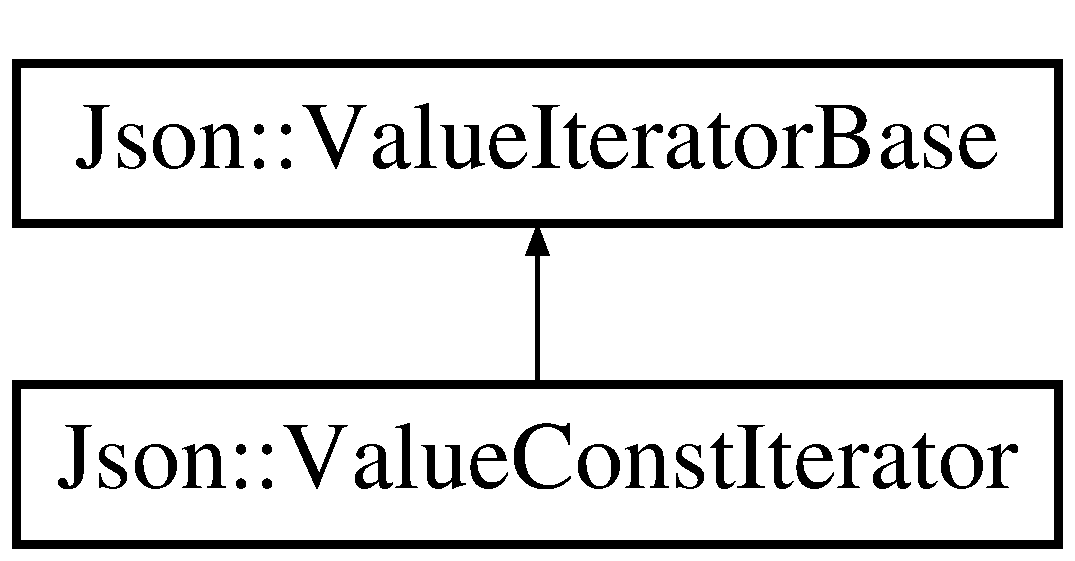
\includegraphics[height=2.000000cm]{class_json_1_1_value_const_iterator}
\end{center}
\end{figure}
\subsection*{Public Types}
\begin{DoxyCompactItemize}
\item 
\hypertarget{class_json_1_1_value_const_iterator_a8685219d214dbd2b763357ae94fb0f27}{typedef unsigned int {\bfseries size\-\_\-t}}\label{class_json_1_1_value_const_iterator_a8685219d214dbd2b763357ae94fb0f27}

\item 
\hypertarget{class_json_1_1_value_const_iterator_a32b36aa9d76e2b48ca74fb6e1979a95a}{typedef int {\bfseries difference\-\_\-type}}\label{class_json_1_1_value_const_iterator_a32b36aa9d76e2b48ca74fb6e1979a95a}

\item 
\hypertarget{class_json_1_1_value_const_iterator_aa9b05c6a37cd352ea1ee6e13b816f709}{typedef const \hyperlink{class_json_1_1_value}{Value} \& {\bfseries reference}}\label{class_json_1_1_value_const_iterator_aa9b05c6a37cd352ea1ee6e13b816f709}

\item 
\hypertarget{class_json_1_1_value_const_iterator_a400136bd8bc09e9fddec0785fa2cff14}{typedef const \hyperlink{class_json_1_1_value}{Value} $\ast$ {\bfseries pointer}}\label{class_json_1_1_value_const_iterator_a400136bd8bc09e9fddec0785fa2cff14}

\item 
\hypertarget{class_json_1_1_value_const_iterator_a0c2e33e7eb5a80dd8709fb28ece83933}{typedef \hyperlink{class_json_1_1_value_const_iterator}{Value\-Const\-Iterator} {\bfseries Self\-Type}}\label{class_json_1_1_value_const_iterator_a0c2e33e7eb5a80dd8709fb28ece83933}

\end{DoxyCompactItemize}
\subsection*{Public Member Functions}
\begin{DoxyCompactItemize}
\item 
\hypertarget{class_json_1_1_value_const_iterator_ad1b1c11f8d7fb22d4d3c231915f2b15b}{\hyperlink{class_json_1_1_value_iterator_base}{Self\-Type} \& {\bfseries operator=} (const \hyperlink{class_json_1_1_value_iterator_base}{Value\-Iterator\-Base} \&other)}\label{class_json_1_1_value_const_iterator_ad1b1c11f8d7fb22d4d3c231915f2b15b}

\item 
\hypertarget{class_json_1_1_value_const_iterator_ab3f0c2edbfc8f7d60645f3d597d05e28}{\hyperlink{class_json_1_1_value_iterator_base}{Self\-Type} {\bfseries operator++} (int)}\label{class_json_1_1_value_const_iterator_ab3f0c2edbfc8f7d60645f3d597d05e28}

\item 
\hypertarget{class_json_1_1_value_const_iterator_a94935961e9331c6f7b907b05ec8df75e}{\hyperlink{class_json_1_1_value_iterator_base}{Self\-Type} {\bfseries operator-\/-\/} (int)}\label{class_json_1_1_value_const_iterator_a94935961e9331c6f7b907b05ec8df75e}

\item 
\hypertarget{class_json_1_1_value_const_iterator_a31415e44e44e56fb2bfda7e8bb784646}{\hyperlink{class_json_1_1_value_iterator_base}{Self\-Type} \& {\bfseries operator-\/-\/} ()}\label{class_json_1_1_value_const_iterator_a31415e44e44e56fb2bfda7e8bb784646}

\item 
\hypertarget{class_json_1_1_value_const_iterator_a2cfe2f7a94a688186efdafb1b181c319}{\hyperlink{class_json_1_1_value_iterator_base}{Self\-Type} \& {\bfseries operator++} ()}\label{class_json_1_1_value_const_iterator_a2cfe2f7a94a688186efdafb1b181c319}

\item 
\hypertarget{class_json_1_1_value_const_iterator_aeb44153d71c61ac9397a84d5ecc244c5}{\hyperlink{class_json_1_1_value}{reference} {\bfseries operator$\ast$} () const }\label{class_json_1_1_value_const_iterator_aeb44153d71c61ac9397a84d5ecc244c5}

\end{DoxyCompactItemize}
\subsection*{Friends}
\begin{DoxyCompactItemize}
\item 
\hypertarget{class_json_1_1_value_const_iterator_aeceedf6e1a7d48a588516ce2b1983d6f}{class {\bfseries Value}}\label{class_json_1_1_value_const_iterator_aeceedf6e1a7d48a588516ce2b1983d6f}

\end{DoxyCompactItemize}
\subsection*{Additional Inherited Members}


\subsection{Detailed Description}
const iterator for object and array value. 



The documentation for this class was generated from the following files\-:\begin{DoxyCompactItemize}
\item 
include/json/json.\-h\item 
src/jsoncpp.\-cpp\end{DoxyCompactItemize}

\hypertarget{class_json_1_1_value_iterator}{\section{Json\-:\-:Value\-Iterator Class Reference}
\label{class_json_1_1_value_iterator}\index{Json\-::\-Value\-Iterator@{Json\-::\-Value\-Iterator}}
}


Iterator for object and array value.  




{\ttfamily \#include $<$json.\-h$>$}

Inheritance diagram for Json\-:\-:Value\-Iterator\-:\begin{figure}[H]
\begin{center}
\leavevmode
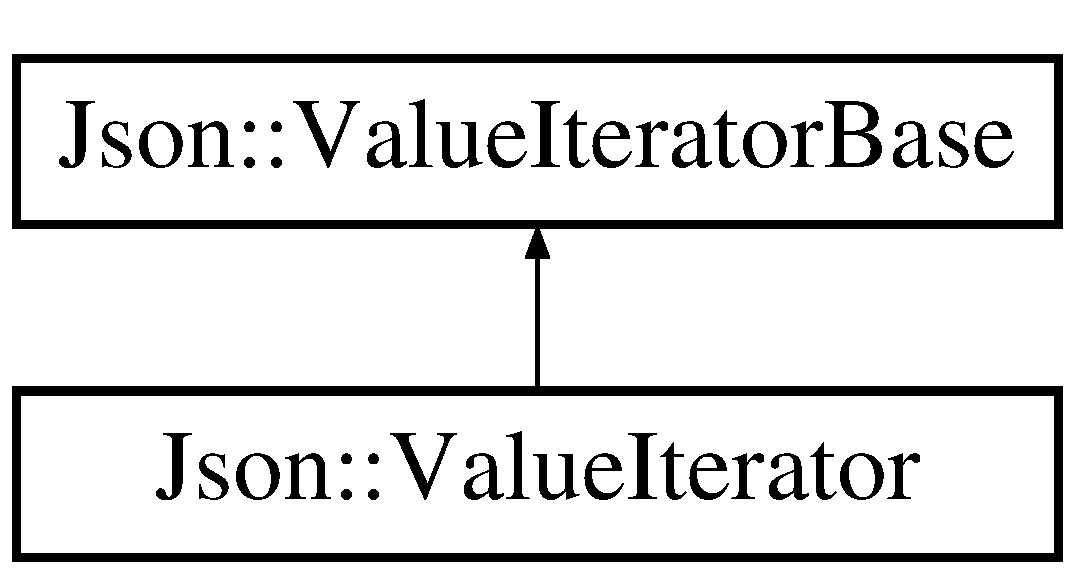
\includegraphics[height=2.000000cm]{class_json_1_1_value_iterator}
\end{center}
\end{figure}
\subsection*{Public Types}
\begin{DoxyCompactItemize}
\item 
\hypertarget{class_json_1_1_value_iterator_a308b8932ffc83eaa9d12dadd5c11a7dd}{typedef unsigned int {\bfseries size\-\_\-t}}\label{class_json_1_1_value_iterator_a308b8932ffc83eaa9d12dadd5c11a7dd}

\item 
\hypertarget{class_json_1_1_value_iterator_a2be1a9aa60bbfc8812e9dd1a7f1a8786}{typedef int {\bfseries difference\-\_\-type}}\label{class_json_1_1_value_iterator_a2be1a9aa60bbfc8812e9dd1a7f1a8786}

\item 
\hypertarget{class_json_1_1_value_iterator_ae87929b4567aa00372cf602c43b57160}{typedef \hyperlink{class_json_1_1_value}{Value} \& {\bfseries reference}}\label{class_json_1_1_value_iterator_ae87929b4567aa00372cf602c43b57160}

\item 
\hypertarget{class_json_1_1_value_iterator_acec45feb1ef1f3bf81240157d06d5432}{typedef \hyperlink{class_json_1_1_value}{Value} $\ast$ {\bfseries pointer}}\label{class_json_1_1_value_iterator_acec45feb1ef1f3bf81240157d06d5432}

\item 
\hypertarget{class_json_1_1_value_iterator_a23357670fdad61792670d86f62db7e16}{typedef \hyperlink{class_json_1_1_value_iterator}{Value\-Iterator} {\bfseries Self\-Type}}\label{class_json_1_1_value_iterator_a23357670fdad61792670d86f62db7e16}

\end{DoxyCompactItemize}
\subsection*{Public Member Functions}
\begin{DoxyCompactItemize}
\item 
\hypertarget{class_json_1_1_value_iterator_aa85aa208670891670392259efa0143bb}{{\bfseries Value\-Iterator} (const \hyperlink{class_json_1_1_value_const_iterator}{Value\-Const\-Iterator} \&other)}\label{class_json_1_1_value_iterator_aa85aa208670891670392259efa0143bb}

\item 
\hypertarget{class_json_1_1_value_iterator_a7d5e58a9a4a553968acdf3064b39d21c}{{\bfseries Value\-Iterator} (const \hyperlink{class_json_1_1_value_iterator}{Value\-Iterator} \&other)}\label{class_json_1_1_value_iterator_a7d5e58a9a4a553968acdf3064b39d21c}

\item 
\hypertarget{class_json_1_1_value_iterator_a8e23312b1db874f7e403fd7e76611bdc}{\hyperlink{class_json_1_1_value_iterator_base}{Self\-Type} \& {\bfseries operator=} (const \hyperlink{class_json_1_1_value_iterator_base}{Self\-Type} \&other)}\label{class_json_1_1_value_iterator_a8e23312b1db874f7e403fd7e76611bdc}

\item 
\hypertarget{class_json_1_1_value_iterator_abcf4ddd994a010742cd4a436d65acd08}{\hyperlink{class_json_1_1_value_iterator_base}{Self\-Type} {\bfseries operator++} (int)}\label{class_json_1_1_value_iterator_abcf4ddd994a010742cd4a436d65acd08}

\item 
\hypertarget{class_json_1_1_value_iterator_a06d6a29d96caf6af324a53973159e12b}{\hyperlink{class_json_1_1_value_iterator_base}{Self\-Type} {\bfseries operator-\/-\/} (int)}\label{class_json_1_1_value_iterator_a06d6a29d96caf6af324a53973159e12b}

\item 
\hypertarget{class_json_1_1_value_iterator_a811302a868518a0995a9def955df5720}{\hyperlink{class_json_1_1_value_iterator_base}{Self\-Type} \& {\bfseries operator-\/-\/} ()}\label{class_json_1_1_value_iterator_a811302a868518a0995a9def955df5720}

\item 
\hypertarget{class_json_1_1_value_iterator_a92146c46f8249e2b2d12869e70cd4cee}{\hyperlink{class_json_1_1_value_iterator_base}{Self\-Type} \& {\bfseries operator++} ()}\label{class_json_1_1_value_iterator_a92146c46f8249e2b2d12869e70cd4cee}

\item 
\hypertarget{class_json_1_1_value_iterator_aaa5be3457eedf0526a03b8a3b4c7c0a0}{\hyperlink{class_json_1_1_value}{reference} {\bfseries operator$\ast$} () const }\label{class_json_1_1_value_iterator_aaa5be3457eedf0526a03b8a3b4c7c0a0}

\end{DoxyCompactItemize}
\subsection*{Friends}
\begin{DoxyCompactItemize}
\item 
\hypertarget{class_json_1_1_value_iterator_aeceedf6e1a7d48a588516ce2b1983d6f}{class {\bfseries Value}}\label{class_json_1_1_value_iterator_aeceedf6e1a7d48a588516ce2b1983d6f}

\end{DoxyCompactItemize}
\subsection*{Additional Inherited Members}


\subsection{Detailed Description}
Iterator for object and array value. 

The documentation for this class was generated from the following files\-:\begin{DoxyCompactItemize}
\item 
include/json/json.\-h\item 
src/jsoncpp.\-cpp\end{DoxyCompactItemize}

\hypertarget{class_json_1_1_value_iterator_base}{\section{Json\-:\-:Value\-Iterator\-Base Class Reference}
\label{class_json_1_1_value_iterator_base}\index{Json\-::\-Value\-Iterator\-Base@{Json\-::\-Value\-Iterator\-Base}}
}


base class for \hyperlink{class_json_1_1_value}{Value} iterators.  




{\ttfamily \#include $<$json.\-h$>$}

Inheritance diagram for Json\-:\-:Value\-Iterator\-Base\-:\begin{figure}[H]
\begin{center}
\leavevmode
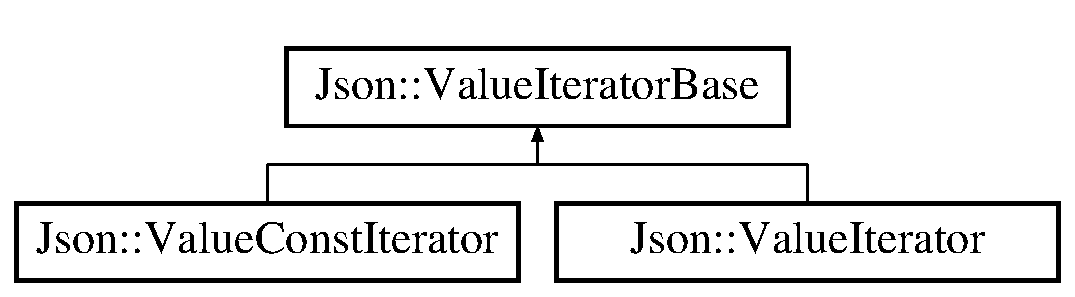
\includegraphics[height=2.000000cm]{class_json_1_1_value_iterator_base}
\end{center}
\end{figure}
\subsection*{Public Types}
\begin{DoxyCompactItemize}
\item 
\hypertarget{class_json_1_1_value_iterator_base_a9d3a3c7ce5cdefe23cb486239cf07bb5}{typedef unsigned int {\bfseries size\-\_\-t}}\label{class_json_1_1_value_iterator_base_a9d3a3c7ce5cdefe23cb486239cf07bb5}

\item 
\hypertarget{class_json_1_1_value_iterator_base_a4e44bf8cbd17ec8d6e2c185904a15ebd}{typedef int {\bfseries difference\-\_\-type}}\label{class_json_1_1_value_iterator_base_a4e44bf8cbd17ec8d6e2c185904a15ebd}

\item 
\hypertarget{class_json_1_1_value_iterator_base_a9d2a940d03ea06d20d972f41a89149ee}{typedef \hyperlink{class_json_1_1_value_iterator_base}{Value\-Iterator\-Base} {\bfseries Self\-Type}}\label{class_json_1_1_value_iterator_base_a9d2a940d03ea06d20d972f41a89149ee}

\end{DoxyCompactItemize}
\subsection*{Public Member Functions}
\begin{DoxyCompactItemize}
\item 
\hypertarget{class_json_1_1_value_iterator_base_a640e990e5f03a96fd650122a2906f59d}{{\bfseries Value\-Iterator\-Base} (const Value\-::\-Object\-Values\-::iterator \&current)}\label{class_json_1_1_value_iterator_base_a640e990e5f03a96fd650122a2906f59d}

\item 
\hypertarget{class_json_1_1_value_iterator_base_afc656672ac28502f640ade32c38c1b56}{bool {\bfseries operator==} (const \hyperlink{class_json_1_1_value_iterator_base}{Self\-Type} \&other) const }\label{class_json_1_1_value_iterator_base_afc656672ac28502f640ade32c38c1b56}

\item 
\hypertarget{class_json_1_1_value_iterator_base_a18c2dd42e0bb989ace141bfe9de52792}{bool {\bfseries operator!=} (const \hyperlink{class_json_1_1_value_iterator_base}{Self\-Type} \&other) const }\label{class_json_1_1_value_iterator_base_a18c2dd42e0bb989ace141bfe9de52792}

\item 
\hypertarget{class_json_1_1_value_iterator_base_ab786787fcad68ca5e8745aaf520fa17f}{difference\-\_\-type {\bfseries operator-\/} (const \hyperlink{class_json_1_1_value_iterator_base}{Self\-Type} \&other) const }\label{class_json_1_1_value_iterator_base_ab786787fcad68ca5e8745aaf520fa17f}

\item 
\hypertarget{class_json_1_1_value_iterator_base_aa2ff5e79fc96acd4c3cd288e92614fc7}{\hyperlink{class_json_1_1_value}{Value} \hyperlink{class_json_1_1_value_iterator_base_aa2ff5e79fc96acd4c3cd288e92614fc7}{key} () const }\label{class_json_1_1_value_iterator_base_aa2ff5e79fc96acd4c3cd288e92614fc7}

\begin{DoxyCompactList}\small\item\em Return either the index or the member name of the referenced value as a \hyperlink{class_json_1_1_value}{Value}. \end{DoxyCompactList}\item 
\hypertarget{class_json_1_1_value_iterator_base_aa90591f5f7f8d2f06cc4605816b53738}{U\-Int \hyperlink{class_json_1_1_value_iterator_base_aa90591f5f7f8d2f06cc4605816b53738}{index} () const }\label{class_json_1_1_value_iterator_base_aa90591f5f7f8d2f06cc4605816b53738}

\begin{DoxyCompactList}\small\item\em Return the index of the referenced \hyperlink{class_json_1_1_value}{Value}. -\/1 if it is not an array\-Value. \end{DoxyCompactList}\item 
\hypertarget{class_json_1_1_value_iterator_base_a83768d87c608c8d1133de8721eefc31b}{const char $\ast$ \hyperlink{class_json_1_1_value_iterator_base_a83768d87c608c8d1133de8721eefc31b}{member\-Name} () const }\label{class_json_1_1_value_iterator_base_a83768d87c608c8d1133de8721eefc31b}

\begin{DoxyCompactList}\small\item\em Return the member name of the referenced \hyperlink{class_json_1_1_value}{Value}. \char`\"{}\char`\"{} if it is not an object\-Value. \end{DoxyCompactList}\end{DoxyCompactItemize}
\subsection*{Protected Member Functions}
\begin{DoxyCompactItemize}
\item 
\hypertarget{class_json_1_1_value_iterator_base_a40a20c65abc423a26e3aae68d9a0525c}{\hyperlink{class_json_1_1_value}{Value} \& {\bfseries deref} () const }\label{class_json_1_1_value_iterator_base_a40a20c65abc423a26e3aae68d9a0525c}

\item 
\hypertarget{class_json_1_1_value_iterator_base_afe58f9534e1fd2033419fd9fe244551e}{void {\bfseries increment} ()}\label{class_json_1_1_value_iterator_base_afe58f9534e1fd2033419fd9fe244551e}

\item 
\hypertarget{class_json_1_1_value_iterator_base_affc8cf5ff54a9f432cc693362c153fa6}{void {\bfseries decrement} ()}\label{class_json_1_1_value_iterator_base_affc8cf5ff54a9f432cc693362c153fa6}

\item 
\hypertarget{class_json_1_1_value_iterator_base_ad6c553b249e89e3dc9933e100ccbe064}{difference\-\_\-type {\bfseries compute\-Distance} (const \hyperlink{class_json_1_1_value_iterator_base}{Self\-Type} \&other) const }\label{class_json_1_1_value_iterator_base_ad6c553b249e89e3dc9933e100ccbe064}

\item 
\hypertarget{class_json_1_1_value_iterator_base_a21820d6ee564e541bd118b21e4741962}{bool {\bfseries is\-Equal} (const \hyperlink{class_json_1_1_value_iterator_base}{Self\-Type} \&other) const }\label{class_json_1_1_value_iterator_base_a21820d6ee564e541bd118b21e4741962}

\item 
\hypertarget{class_json_1_1_value_iterator_base_a496e6aba44808433ec5858c178be5719}{void {\bfseries copy} (const \hyperlink{class_json_1_1_value_iterator_base}{Self\-Type} \&other)}\label{class_json_1_1_value_iterator_base_a496e6aba44808433ec5858c178be5719}

\end{DoxyCompactItemize}


\subsection{Detailed Description}
base class for \hyperlink{class_json_1_1_value}{Value} iterators. 



The documentation for this class was generated from the following files\-:\begin{DoxyCompactItemize}
\item 
include/json/json.\-h\item 
src/jsoncpp.\-cpp\end{DoxyCompactItemize}

\hypertarget{struct_value_list}{\section{Value\-List Struct Reference}
\label{struct_value_list}\index{Value\-List@{Value\-List}}
}
\subsection*{Public Attributes}
\begin{DoxyCompactItemize}
\item 
\hypertarget{struct_value_list_a6119dd8fd520ba00ebbe9425be94184b}{\hyperlink{struct_expr_list}{Expr\-List} $\ast$ {\bfseries p\-List}}\label{struct_value_list_a6119dd8fd520ba00ebbe9425be94184b}

\item 
\hypertarget{struct_value_list_a1cce43c59968143faef1a9e457fad59a}{\hyperlink{struct_select}{Select} $\ast$ {\bfseries p\-Select}}\label{struct_value_list_a1cce43c59968143faef1a9e457fad59a}

\end{DoxyCompactItemize}


The documentation for this struct was generated from the following file\-:\begin{DoxyCompactItemize}
\item 
src/sqlite3.\-c\end{DoxyCompactItemize}

\hypertarget{struct_vdbe}{\section{Vdbe Struct Reference}
\label{struct_vdbe}\index{Vdbe@{Vdbe}}
}
\subsection*{Public Attributes}
\begin{DoxyCompactItemize}
\item 
\hypertarget{struct_vdbe_a495366101a593999f4d2ed905e839029}{\hyperlink{structsqlite3}{sqlite3} $\ast$ {\bfseries db}}\label{struct_vdbe_a495366101a593999f4d2ed905e839029}

\item 
\hypertarget{struct_vdbe_a1ba82f08947b275dd72a3e3095ad02d5}{\hyperlink{struct_vdbe_op}{Op} $\ast$ {\bfseries a\-Op}}\label{struct_vdbe_a1ba82f08947b275dd72a3e3095ad02d5}

\item 
\hypertarget{struct_vdbe_ac36776c53b6ec9054a2826ec83f29953}{\hyperlink{struct_mem}{Mem} $\ast$ {\bfseries a\-Mem}}\label{struct_vdbe_ac36776c53b6ec9054a2826ec83f29953}

\item 
\hypertarget{struct_vdbe_a74fd4612c55ac2fde475096a4d2605b5}{\hyperlink{struct_mem}{Mem} $\ast$$\ast$ {\bfseries ap\-Arg}}\label{struct_vdbe_a74fd4612c55ac2fde475096a4d2605b5}

\item 
\hypertarget{struct_vdbe_a900f557143e7d2ab8c560f7ada66d0f7}{\hyperlink{struct_mem}{Mem} $\ast$ {\bfseries a\-Col\-Name}}\label{struct_vdbe_a900f557143e7d2ab8c560f7ada66d0f7}

\item 
\hypertarget{struct_vdbe_a0dec47b8d8c481df2b73d5bbf9cdde11}{\hyperlink{struct_mem}{Mem} $\ast$ {\bfseries p\-Result\-Set}}\label{struct_vdbe_a0dec47b8d8c481df2b73d5bbf9cdde11}

\item 
\hypertarget{struct_vdbe_a10a19309607617a75d3722219d3c7615}{int {\bfseries n\-Mem}}\label{struct_vdbe_a10a19309607617a75d3722219d3c7615}

\item 
\hypertarget{struct_vdbe_a81e72e6812c71e13651f81cc3a6ca1d0}{int {\bfseries n\-Op}}\label{struct_vdbe_a81e72e6812c71e13651f81cc3a6ca1d0}

\item 
\hypertarget{struct_vdbe_aa52020050ea42e10ad8be8ebdf470850}{int {\bfseries n\-Op\-Alloc}}\label{struct_vdbe_aa52020050ea42e10ad8be8ebdf470850}

\item 
\hypertarget{struct_vdbe_ae74cf1db577889e4f7ee669d613939a9}{int {\bfseries n\-Label}}\label{struct_vdbe_ae74cf1db577889e4f7ee669d613939a9}

\item 
\hypertarget{struct_vdbe_a8d9c9a70f5a5ffd037cc29cd3d3815b2}{int $\ast$ {\bfseries a\-Label}}\label{struct_vdbe_a8d9c9a70f5a5ffd037cc29cd3d3815b2}

\item 
\hypertarget{struct_vdbe_a525830c709542b280d11c764e9a9994a}{u16 {\bfseries n\-Res\-Column}}\label{struct_vdbe_a525830c709542b280d11c764e9a9994a}

\item 
\hypertarget{struct_vdbe_adf7c35ba970bfc5f6e06a9f8248d5a32}{u16 {\bfseries n\-Cursor}}\label{struct_vdbe_adf7c35ba970bfc5f6e06a9f8248d5a32}

\item 
\hypertarget{struct_vdbe_a01c61f8cafa6ad3eaafcc85c6f53f8ef}{u32 {\bfseries magic}}\label{struct_vdbe_a01c61f8cafa6ad3eaafcc85c6f53f8ef}

\item 
\hypertarget{struct_vdbe_add7679059dd1e3cd483ddcb9153ca844}{char $\ast$ {\bfseries z\-Err\-Msg}}\label{struct_vdbe_add7679059dd1e3cd483ddcb9153ca844}

\item 
\hypertarget{struct_vdbe_a2afc3b6cd2f5b38d991148b809b3c53f}{\hyperlink{struct_vdbe}{Vdbe} $\ast$ {\bfseries p\-Prev}}\label{struct_vdbe_a2afc3b6cd2f5b38d991148b809b3c53f}

\item 
\hypertarget{struct_vdbe_a9d52c1a2d64f132c6994eeac00063df9}{\hyperlink{struct_vdbe}{Vdbe} $\ast$ {\bfseries p\-Next}}\label{struct_vdbe_a9d52c1a2d64f132c6994eeac00063df9}

\item 
\hypertarget{struct_vdbe_a8bd1b6ecdc16918e10ee1ae90b4e19ef}{\hyperlink{struct_vdbe_cursor}{Vdbe\-Cursor} $\ast$$\ast$ {\bfseries ap\-Csr}}\label{struct_vdbe_a8bd1b6ecdc16918e10ee1ae90b4e19ef}

\item 
\hypertarget{struct_vdbe_a8877b72591926e3597fa93e22f84b99c}{\hyperlink{struct_mem}{Mem} $\ast$ {\bfseries a\-Var}}\label{struct_vdbe_a8877b72591926e3597fa93e22f84b99c}

\item 
\hypertarget{struct_vdbe_af3c62ca5eee6b2549c97a6bb87fb2f54}{char $\ast$$\ast$ {\bfseries az\-Var}}\label{struct_vdbe_af3c62ca5eee6b2549c97a6bb87fb2f54}

\item 
\hypertarget{struct_vdbe_a2acd8f1fa65e19eb48fc62ddb6cb7569}{yn\-Var {\bfseries n\-Var}}\label{struct_vdbe_a2acd8f1fa65e19eb48fc62ddb6cb7569}

\item 
\hypertarget{struct_vdbe_aacefce2bccaad230767304a56986007d}{yn\-Var {\bfseries nz\-Var}}\label{struct_vdbe_aacefce2bccaad230767304a56986007d}

\item 
\hypertarget{struct_vdbe_ace5722464070f2055f536b737955b9ad}{u32 {\bfseries cache\-Ctr}}\label{struct_vdbe_ace5722464070f2055f536b737955b9ad}

\item 
\hypertarget{struct_vdbe_ae25264a36877487fb58814608a46689c}{int {\bfseries pc}}\label{struct_vdbe_ae25264a36877487fb58814608a46689c}

\item 
\hypertarget{struct_vdbe_af82fb0227a5b8db9d3b9bdb03964a4a0}{int {\bfseries rc}}\label{struct_vdbe_af82fb0227a5b8db9d3b9bdb03964a4a0}

\item 
\hypertarget{struct_vdbe_ab2fde65c1d4728e92d100ce21313dcd3}{u8 {\bfseries error\-Action}}\label{struct_vdbe_ab2fde65c1d4728e92d100ce21313dcd3}

\item 
\hypertarget{struct_vdbe_a679ac87f7b835982cd7c1990fbc3605b}{u8 {\bfseries min\-Write\-File\-Format}}\label{struct_vdbe_a679ac87f7b835982cd7c1990fbc3605b}

\item 
\hypertarget{struct_vdbe_a9ea665c14b97cccb7ce08c129f5b38b6}{bft {\bfseries explain}\-:2}\label{struct_vdbe_a9ea665c14b97cccb7ce08c129f5b38b6}

\item 
\hypertarget{struct_vdbe_a95287183ab74eadc963739405bb6e482}{bft {\bfseries in\-Vtab\-Method}\-:2}\label{struct_vdbe_a95287183ab74eadc963739405bb6e482}

\item 
\hypertarget{struct_vdbe_a2eafa7984a14e56f31e46fa4b90b0582}{bft {\bfseries change\-Cnt\-On}\-:1}\label{struct_vdbe_a2eafa7984a14e56f31e46fa4b90b0582}

\item 
\hypertarget{struct_vdbe_a1958421b98e6b660a86f58300e2d207d}{bft {\bfseries expired}\-:1}\label{struct_vdbe_a1958421b98e6b660a86f58300e2d207d}

\item 
\hypertarget{struct_vdbe_a8a721c9051a913cc59d546de68dfd91c}{bft {\bfseries run\-Only\-Once}\-:1}\label{struct_vdbe_a8a721c9051a913cc59d546de68dfd91c}

\item 
\hypertarget{struct_vdbe_a4d1f6dfd3a6c17fa28e9ad1eac8e4839}{bft {\bfseries uses\-Stmt\-Journal}\-:1}\label{struct_vdbe_a4d1f6dfd3a6c17fa28e9ad1eac8e4839}

\item 
\hypertarget{struct_vdbe_accc1c66c5ff9524a8ad3051d754e798c}{bft {\bfseries read\-Only}\-:1}\label{struct_vdbe_accc1c66c5ff9524a8ad3051d754e798c}

\item 
\hypertarget{struct_vdbe_abe5efc12c758bb2d7f8ecd477cfa4952}{bft {\bfseries is\-Prepare\-V2}\-:1}\label{struct_vdbe_abe5efc12c758bb2d7f8ecd477cfa4952}

\item 
\hypertarget{struct_vdbe_aacf1f57675f3c37a924aba5c74e035ea}{bft {\bfseries doing\-Rerun}\-:1}\label{struct_vdbe_aacf1f57675f3c37a924aba5c74e035ea}

\item 
\hypertarget{struct_vdbe_a59d1ece56f21e260cdd0fef936242b28}{int {\bfseries n\-Change}}\label{struct_vdbe_a59d1ece56f21e260cdd0fef936242b28}

\item 
\hypertarget{struct_vdbe_a82cb99588b3650e6f10583275392ce7c}{y\-Db\-Mask {\bfseries btree\-Mask}}\label{struct_vdbe_a82cb99588b3650e6f10583275392ce7c}

\item 
\hypertarget{struct_vdbe_a7de4b1df727c3d2d32778a77f5c5dd68}{y\-Db\-Mask {\bfseries lock\-Mask}}\label{struct_vdbe_a7de4b1df727c3d2d32778a77f5c5dd68}

\item 
\hypertarget{struct_vdbe_ae2b5893f3d37e004acac58bffee1a229}{int {\bfseries i\-Statement}}\label{struct_vdbe_ae2b5893f3d37e004acac58bffee1a229}

\item 
\hypertarget{struct_vdbe_a9838a4909a9a19ead07ca7482a472665}{int {\bfseries a\-Counter} \mbox{[}3\mbox{]}}\label{struct_vdbe_a9838a4909a9a19ead07ca7482a472665}

\item 
\hypertarget{struct_vdbe_a1de76a5c58ed36608a163bfdc2e9e8b7}{i64 {\bfseries start\-Time}}\label{struct_vdbe_a1de76a5c58ed36608a163bfdc2e9e8b7}

\item 
\hypertarget{struct_vdbe_a7f46ff5e6b3dbf3632e941e27c82a485}{i64 {\bfseries n\-Fk\-Constraint}}\label{struct_vdbe_a7f46ff5e6b3dbf3632e941e27c82a485}

\item 
\hypertarget{struct_vdbe_ab6a710cd4796c6adc8967e7b5bf35757}{i64 {\bfseries n\-Stmt\-Def\-Cons}}\label{struct_vdbe_ab6a710cd4796c6adc8967e7b5bf35757}

\item 
\hypertarget{struct_vdbe_a5a61fd8f84ae0399ef73327e48048ae9}{char $\ast$ {\bfseries z\-Sql}}\label{struct_vdbe_a5a61fd8f84ae0399ef73327e48048ae9}

\item 
\hypertarget{struct_vdbe_a68dcaae5d4f061da3d7bb96c120fe9a4}{void $\ast$ {\bfseries p\-Free}}\label{struct_vdbe_a68dcaae5d4f061da3d7bb96c120fe9a4}

\item 
\hypertarget{struct_vdbe_afd754aaedd6cd5b229fbeff33177fe04}{\hyperlink{struct_vdbe_frame}{Vdbe\-Frame} $\ast$ {\bfseries p\-Frame}}\label{struct_vdbe_afd754aaedd6cd5b229fbeff33177fe04}

\item 
\hypertarget{struct_vdbe_ab8f22136c8bdb4c02962a1ae081e9116}{\hyperlink{struct_vdbe_frame}{Vdbe\-Frame} $\ast$ {\bfseries p\-Del\-Frame}}\label{struct_vdbe_ab8f22136c8bdb4c02962a1ae081e9116}

\item 
\hypertarget{struct_vdbe_a27fbd083a0335ac2b332d37ea2b90bdc}{int {\bfseries n\-Frame}}\label{struct_vdbe_a27fbd083a0335ac2b332d37ea2b90bdc}

\item 
\hypertarget{struct_vdbe_a5e22eedb6ee963a0bcf27fc9fd8b8e43}{u32 {\bfseries expmask}}\label{struct_vdbe_a5e22eedb6ee963a0bcf27fc9fd8b8e43}

\item 
\hypertarget{struct_vdbe_a9239ea72573142101328be15c90de62b}{\hyperlink{struct_sub_program}{Sub\-Program} $\ast$ {\bfseries p\-Program}}\label{struct_vdbe_a9239ea72573142101328be15c90de62b}

\item 
\hypertarget{struct_vdbe_a55e673e0ba209872b23c64c87b36bf56}{int {\bfseries n\-Once\-Flag}}\label{struct_vdbe_a55e673e0ba209872b23c64c87b36bf56}

\item 
\hypertarget{struct_vdbe_a015887ad1c7c597fb78dc08060cb3dc6}{u8 $\ast$ {\bfseries a\-Once\-Flag}}\label{struct_vdbe_a015887ad1c7c597fb78dc08060cb3dc6}

\end{DoxyCompactItemize}


The documentation for this struct was generated from the following file\-:\begin{DoxyCompactItemize}
\item 
src/sqlite3.\-c\end{DoxyCompactItemize}

\hypertarget{struct_vdbe_cursor}{\section{Vdbe\-Cursor Struct Reference}
\label{struct_vdbe_cursor}\index{Vdbe\-Cursor@{Vdbe\-Cursor}}
}
\subsection*{Public Attributes}
\begin{DoxyCompactItemize}
\item 
\hypertarget{struct_vdbe_cursor_a9ecb4ab9f7374f92da69f03fc336c293}{\hyperlink{struct_bt_cursor}{Bt\-Cursor} $\ast$ {\bfseries p\-Cursor}}\label{struct_vdbe_cursor_a9ecb4ab9f7374f92da69f03fc336c293}

\item 
\hypertarget{struct_vdbe_cursor_a287db3fe6d84102fad3d69494b565e9b}{\hyperlink{struct_btree}{Btree} $\ast$ {\bfseries p\-Bt}}\label{struct_vdbe_cursor_a287db3fe6d84102fad3d69494b565e9b}

\item 
\hypertarget{struct_vdbe_cursor_a72a6c26ab2ab2ad699dfb45703ea4765}{\hyperlink{struct_key_info}{Key\-Info} $\ast$ {\bfseries p\-Key\-Info}}\label{struct_vdbe_cursor_a72a6c26ab2ab2ad699dfb45703ea4765}

\item 
\hypertarget{struct_vdbe_cursor_a1215b7b0d1bbd882d6bfb8b118712d89}{int {\bfseries i\-Db}}\label{struct_vdbe_cursor_a1215b7b0d1bbd882d6bfb8b118712d89}

\item 
\hypertarget{struct_vdbe_cursor_a8618d7c5669c83856e95b8ef72ef67b7}{int {\bfseries pseudo\-Table\-Reg}}\label{struct_vdbe_cursor_a8618d7c5669c83856e95b8ef72ef67b7}

\item 
\hypertarget{struct_vdbe_cursor_aa115a60e335e738945127141303eaedb}{int {\bfseries n\-Field}}\label{struct_vdbe_cursor_aa115a60e335e738945127141303eaedb}

\item 
\hypertarget{struct_vdbe_cursor_abcc5ef422583a743105243e2a0c7859e}{Bool {\bfseries zeroed}}\label{struct_vdbe_cursor_abcc5ef422583a743105243e2a0c7859e}

\item 
\hypertarget{struct_vdbe_cursor_a2dabf623f6e3c31aa8310c72ec1843bf}{Bool {\bfseries rowid\-Is\-Valid}}\label{struct_vdbe_cursor_a2dabf623f6e3c31aa8310c72ec1843bf}

\item 
\hypertarget{struct_vdbe_cursor_a00d121ca0f21e7381aacb89adf40e8b6}{Bool {\bfseries at\-First}}\label{struct_vdbe_cursor_a00d121ca0f21e7381aacb89adf40e8b6}

\item 
\hypertarget{struct_vdbe_cursor_a067fff911d6d37190785a0cf5ba4fc8e}{Bool {\bfseries use\-Random\-Rowid}}\label{struct_vdbe_cursor_a067fff911d6d37190785a0cf5ba4fc8e}

\item 
\hypertarget{struct_vdbe_cursor_af7c01a62f0445440e4200f7601ab0a15}{Bool {\bfseries null\-Row}}\label{struct_vdbe_cursor_af7c01a62f0445440e4200f7601ab0a15}

\item 
\hypertarget{struct_vdbe_cursor_ad2da7e0fd569b01c89c18e4dff1b335d}{Bool {\bfseries deferred\-Moveto}}\label{struct_vdbe_cursor_ad2da7e0fd569b01c89c18e4dff1b335d}

\item 
\hypertarget{struct_vdbe_cursor_a2c9ae9907e6649324d65d8cbd889806e}{Bool {\bfseries is\-Table}}\label{struct_vdbe_cursor_a2c9ae9907e6649324d65d8cbd889806e}

\item 
\hypertarget{struct_vdbe_cursor_a60a947acdb24b640fe0ff6112d0ae104}{Bool {\bfseries is\-Index}}\label{struct_vdbe_cursor_a60a947acdb24b640fe0ff6112d0ae104}

\item 
\hypertarget{struct_vdbe_cursor_a8d9e802372b801c4eb5aef6340cfa21a}{Bool {\bfseries is\-Ordered}}\label{struct_vdbe_cursor_a8d9e802372b801c4eb5aef6340cfa21a}

\item 
\hypertarget{struct_vdbe_cursor_a1bb8b53ff5eb06047c38da9e7306395b}{Bool {\bfseries is\-Sorter}}\label{struct_vdbe_cursor_a1bb8b53ff5eb06047c38da9e7306395b}

\item 
\hypertarget{struct_vdbe_cursor_a4685dedcbe1777026ae97d9728fed929}{Bool {\bfseries multi\-Pseudo}}\label{struct_vdbe_cursor_a4685dedcbe1777026ae97d9728fed929}

\item 
\hypertarget{struct_vdbe_cursor_a2f58fca4f47a313a461f40a0ac553bf5}{\hyperlink{structsqlite3__vtab__cursor}{sqlite3\-\_\-vtab\-\_\-cursor} $\ast$ {\bfseries p\-Vtab\-Cursor}}\label{struct_vdbe_cursor_a2f58fca4f47a313a461f40a0ac553bf5}

\item 
\hypertarget{struct_vdbe_cursor_ab385a7fa060ff00bbe9e6861bb599505}{const \hyperlink{structsqlite3__module}{sqlite3\-\_\-module} $\ast$ {\bfseries p\-Module}}\label{struct_vdbe_cursor_ab385a7fa060ff00bbe9e6861bb599505}

\item 
\hypertarget{struct_vdbe_cursor_a4f11f0befb0dcf16273cc832ca6d92a5}{i64 {\bfseries seq\-Count}}\label{struct_vdbe_cursor_a4f11f0befb0dcf16273cc832ca6d92a5}

\item 
\hypertarget{struct_vdbe_cursor_af3c157d480c0597ba50aca227eb8e3b8}{i64 {\bfseries moveto\-Target}}\label{struct_vdbe_cursor_af3c157d480c0597ba50aca227eb8e3b8}

\item 
\hypertarget{struct_vdbe_cursor_af2ff971acc308c012c60b1e949c64411}{i64 {\bfseries last\-Rowid}}\label{struct_vdbe_cursor_af2ff971acc308c012c60b1e949c64411}

\item 
\hypertarget{struct_vdbe_cursor_a7e9030a9f4ff8f8161a78dae28a1fe3b}{\hyperlink{struct_vdbe_sorter}{Vdbe\-Sorter} $\ast$ {\bfseries p\-Sorter}}\label{struct_vdbe_cursor_a7e9030a9f4ff8f8161a78dae28a1fe3b}

\item 
\hypertarget{struct_vdbe_cursor_a5eff86e2a9c87dc15956ad362aa03f05}{int {\bfseries seek\-Result}}\label{struct_vdbe_cursor_a5eff86e2a9c87dc15956ad362aa03f05}

\item 
\hypertarget{struct_vdbe_cursor_acf243b5a94a6e5a11341d6fece473c00}{u32 {\bfseries cache\-Status}}\label{struct_vdbe_cursor_acf243b5a94a6e5a11341d6fece473c00}

\item 
\hypertarget{struct_vdbe_cursor_a5c1fa124d7f27a30e14ef0f455955cab}{int {\bfseries payload\-Size}}\label{struct_vdbe_cursor_a5c1fa124d7f27a30e14ef0f455955cab}

\item 
\hypertarget{struct_vdbe_cursor_a6992d2bf9eb8480985aec47dae58f1ab}{u32 $\ast$ {\bfseries a\-Type}}\label{struct_vdbe_cursor_a6992d2bf9eb8480985aec47dae58f1ab}

\item 
\hypertarget{struct_vdbe_cursor_a17431e67b341282aeb6c026cd01ec1e9}{u32 $\ast$ {\bfseries a\-Offset}}\label{struct_vdbe_cursor_a17431e67b341282aeb6c026cd01ec1e9}

\item 
\hypertarget{struct_vdbe_cursor_a6bd10979ffb5d4828967eea1d6e0d2c8}{u8 $\ast$ {\bfseries a\-Row}}\label{struct_vdbe_cursor_a6bd10979ffb5d4828967eea1d6e0d2c8}

\end{DoxyCompactItemize}


The documentation for this struct was generated from the following file\-:\begin{DoxyCompactItemize}
\item 
src/sqlite3.\-c\end{DoxyCompactItemize}

\hypertarget{struct_vdbe_frame}{\section{Vdbe\-Frame Struct Reference}
\label{struct_vdbe_frame}\index{Vdbe\-Frame@{Vdbe\-Frame}}
}
\subsection*{Public Attributes}
\begin{DoxyCompactItemize}
\item 
\hypertarget{struct_vdbe_frame_a2f6258356959c94398d1d006a740c4ce}{\hyperlink{struct_vdbe}{Vdbe} $\ast$ {\bfseries v}}\label{struct_vdbe_frame_a2f6258356959c94398d1d006a740c4ce}

\item 
\hypertarget{struct_vdbe_frame_afb11d8aa920f34720333f52737375d59}{\hyperlink{struct_vdbe_frame}{Vdbe\-Frame} $\ast$ {\bfseries p\-Parent}}\label{struct_vdbe_frame_afb11d8aa920f34720333f52737375d59}

\item 
\hypertarget{struct_vdbe_frame_a0e5670c52e8eeb7e66bf1e3bff8ce2b5}{\hyperlink{struct_vdbe_op}{Op} $\ast$ {\bfseries a\-Op}}\label{struct_vdbe_frame_a0e5670c52e8eeb7e66bf1e3bff8ce2b5}

\item 
\hypertarget{struct_vdbe_frame_a98b9eabf633e77d4ae2dfe9d13a43fdf}{\hyperlink{struct_mem}{Mem} $\ast$ {\bfseries a\-Mem}}\label{struct_vdbe_frame_a98b9eabf633e77d4ae2dfe9d13a43fdf}

\item 
\hypertarget{struct_vdbe_frame_a92608c14f2aa3be81e65d59000ef8bd8}{u8 $\ast$ {\bfseries a\-Once\-Flag}}\label{struct_vdbe_frame_a92608c14f2aa3be81e65d59000ef8bd8}

\item 
\hypertarget{struct_vdbe_frame_a5d373b3a195dbd1a31f5aa0dbe1822ee}{\hyperlink{struct_vdbe_cursor}{Vdbe\-Cursor} $\ast$$\ast$ {\bfseries ap\-Csr}}\label{struct_vdbe_frame_a5d373b3a195dbd1a31f5aa0dbe1822ee}

\item 
\hypertarget{struct_vdbe_frame_a11de10011ea2164995c6b616bba8a576}{void $\ast$ {\bfseries token}}\label{struct_vdbe_frame_a11de10011ea2164995c6b616bba8a576}

\item 
\hypertarget{struct_vdbe_frame_af655193217fb53c7acab9d24c94344aa}{i64 {\bfseries last\-Rowid}}\label{struct_vdbe_frame_af655193217fb53c7acab9d24c94344aa}

\item 
\hypertarget{struct_vdbe_frame_af6d743df3f86ff683959562c1b615655}{u16 {\bfseries n\-Cursor}}\label{struct_vdbe_frame_af6d743df3f86ff683959562c1b615655}

\item 
\hypertarget{struct_vdbe_frame_aed0e6d8cb1908580a3c2aca04516b46c}{int {\bfseries pc}}\label{struct_vdbe_frame_aed0e6d8cb1908580a3c2aca04516b46c}

\item 
\hypertarget{struct_vdbe_frame_acffd5d53fbb5cb55e257c34a547c1762}{int {\bfseries n\-Op}}\label{struct_vdbe_frame_acffd5d53fbb5cb55e257c34a547c1762}

\item 
\hypertarget{struct_vdbe_frame_ab340f2b5f6d6e09a872f5f8a64fec245}{int {\bfseries n\-Mem}}\label{struct_vdbe_frame_ab340f2b5f6d6e09a872f5f8a64fec245}

\item 
\hypertarget{struct_vdbe_frame_a04707991a2907a48a1c3b76f3da4d26b}{int {\bfseries n\-Once\-Flag}}\label{struct_vdbe_frame_a04707991a2907a48a1c3b76f3da4d26b}

\item 
\hypertarget{struct_vdbe_frame_a833bdf519676567bc3a700cdedc6562d}{int {\bfseries n\-Child\-Mem}}\label{struct_vdbe_frame_a833bdf519676567bc3a700cdedc6562d}

\item 
\hypertarget{struct_vdbe_frame_a2d2900348092258d12eb71057812429a}{int {\bfseries n\-Child\-Csr}}\label{struct_vdbe_frame_a2d2900348092258d12eb71057812429a}

\item 
\hypertarget{struct_vdbe_frame_a77aacb67d627f4446dd50a795b5a2f0f}{int {\bfseries n\-Change}}\label{struct_vdbe_frame_a77aacb67d627f4446dd50a795b5a2f0f}

\end{DoxyCompactItemize}


The documentation for this struct was generated from the following file\-:\begin{DoxyCompactItemize}
\item 
src/sqlite3.\-c\end{DoxyCompactItemize}

\hypertarget{struct_vdbe_func}{\section{Vdbe\-Func Struct Reference}
\label{struct_vdbe_func}\index{Vdbe\-Func@{Vdbe\-Func}}
}
\subsection*{Classes}
\begin{DoxyCompactItemize}
\item 
struct \hyperlink{struct_vdbe_func_1_1_aux_data}{Aux\-Data}
\end{DoxyCompactItemize}
\subsection*{Public Attributes}
\begin{DoxyCompactItemize}
\item 
\hypertarget{struct_vdbe_func_a73cbc96029bec2f37c7e2a79052a2f65}{\hyperlink{struct_func_def}{Func\-Def} $\ast$ {\bfseries p\-Func}}\label{struct_vdbe_func_a73cbc96029bec2f37c7e2a79052a2f65}

\item 
\hypertarget{struct_vdbe_func_ad78feda4c310ea0bc17b7bba53bccd3c}{int {\bfseries n\-Aux}}\label{struct_vdbe_func_ad78feda4c310ea0bc17b7bba53bccd3c}

\item 
\hypertarget{struct_vdbe_func_abb466d61a0d36b913418460e5922166a}{struct \hyperlink{struct_vdbe_func_1_1_aux_data}{Vdbe\-Func\-::\-Aux\-Data} {\bfseries ap\-Aux} \mbox{[}1\mbox{]}}\label{struct_vdbe_func_abb466d61a0d36b913418460e5922166a}

\end{DoxyCompactItemize}


The documentation for this struct was generated from the following file\-:\begin{DoxyCompactItemize}
\item 
src/sqlite3.\-c\end{DoxyCompactItemize}

\hypertarget{struct_vdbe_op}{\section{Vdbe\-Op Struct Reference}
\label{struct_vdbe_op}\index{Vdbe\-Op@{Vdbe\-Op}}
}
\subsection*{Public Attributes}
\begin{DoxyCompactItemize}
\item 
\hypertarget{struct_vdbe_op_ae12a8e7a8f5f7ba39fa379c9ad287837}{u8 {\bfseries opcode}}\label{struct_vdbe_op_ae12a8e7a8f5f7ba39fa379c9ad287837}

\item 
\hypertarget{struct_vdbe_op_a124dee58d3e0d73c7dfaf811a3311023}{signed char {\bfseries p4type}}\label{struct_vdbe_op_a124dee58d3e0d73c7dfaf811a3311023}

\item 
\hypertarget{struct_vdbe_op_a169a7bbe99a90c26ee01833723750b1d}{u8 {\bfseries opflags}}\label{struct_vdbe_op_a169a7bbe99a90c26ee01833723750b1d}

\item 
\hypertarget{struct_vdbe_op_a5e807981f52d29c06a5b6d4a8f2f4595}{u8 {\bfseries p5}}\label{struct_vdbe_op_a5e807981f52d29c06a5b6d4a8f2f4595}

\item 
\hypertarget{struct_vdbe_op_a17c8326a1e3ac5612d4aaaa88f383b3b}{int {\bfseries p1}}\label{struct_vdbe_op_a17c8326a1e3ac5612d4aaaa88f383b3b}

\item 
\hypertarget{struct_vdbe_op_aba021fa9d30343c16794d9b76d8bffcd}{int {\bfseries p2}}\label{struct_vdbe_op_aba021fa9d30343c16794d9b76d8bffcd}

\item 
\hypertarget{struct_vdbe_op_ad7ef3319da20d5423b8cc5da6995d193}{int {\bfseries p3}}\label{struct_vdbe_op_ad7ef3319da20d5423b8cc5da6995d193}

\item 
\hypertarget{struct_vdbe_op_ad12005effc92477a2fb99b0cadb3b5e0}{\begin{tabbing}
xx\=xx\=xx\=xx\=xx\=xx\=xx\=xx\=xx\=\kill
union \{\\
\>int {\bfseries i}\\
\>void $\ast$ {\bfseries p}\\
\>char $\ast$ {\bfseries z}\\
\>i64 $\ast$ {\bfseries pI64}\\
\>double $\ast$ {\bfseries pReal}\\
\>\hyperlink{struct_func_def}{FuncDef} $\ast$ {\bfseries pFunc}\\
\>\hyperlink{struct_vdbe_func}{VdbeFunc} $\ast$ {\bfseries pVdbeFunc}\\
\>\hyperlink{struct_coll_seq}{CollSeq} $\ast$ {\bfseries pColl}\\
\>\hyperlink{struct_mem}{Mem} $\ast$ {\bfseries pMem}\\
\>\hyperlink{struct_v_table}{VTable} $\ast$ {\bfseries pVtab}\\
\>\hyperlink{struct_key_info}{KeyInfo} $\ast$ {\bfseries pKeyInfo}\\
\>int $\ast$ {\bfseries ai}\\
\>\hyperlink{struct_sub_program}{SubProgram} $\ast$ {\bfseries pProgram}\\
\>int($\ast$ {\bfseries xAdvance} )(\hyperlink{struct_bt_cursor}{BtCursor} $\ast$, int $\ast$)\\
\} {\bfseries p4}}\label{struct_vdbe_op_ad12005effc92477a2fb99b0cadb3b5e0}
\\

\end{tabbing}\end{DoxyCompactItemize}


The documentation for this struct was generated from the following file\-:\begin{DoxyCompactItemize}
\item 
src/sqlite3.\-c\end{DoxyCompactItemize}

\hypertarget{struct_vdbe_op_list}{\section{Vdbe\-Op\-List Struct Reference}
\label{struct_vdbe_op_list}\index{Vdbe\-Op\-List@{Vdbe\-Op\-List}}
}
\subsection*{Public Attributes}
\begin{DoxyCompactItemize}
\item 
\hypertarget{struct_vdbe_op_list_a9c839a619aed99f91cb5e226487be7be}{u8 {\bfseries opcode}}\label{struct_vdbe_op_list_a9c839a619aed99f91cb5e226487be7be}

\item 
\hypertarget{struct_vdbe_op_list_a68641ef4313dfdfafe45b75203c49d5a}{signed char {\bfseries p1}}\label{struct_vdbe_op_list_a68641ef4313dfdfafe45b75203c49d5a}

\item 
\hypertarget{struct_vdbe_op_list_a8493431402f7f91cea81c00e311dc4e1}{signed char {\bfseries p2}}\label{struct_vdbe_op_list_a8493431402f7f91cea81c00e311dc4e1}

\item 
\hypertarget{struct_vdbe_op_list_a584cdaa02042fd5d1bc8cffbdfd9441d}{signed char {\bfseries p3}}\label{struct_vdbe_op_list_a584cdaa02042fd5d1bc8cffbdfd9441d}

\end{DoxyCompactItemize}


The documentation for this struct was generated from the following file\-:\begin{DoxyCompactItemize}
\item 
src/sqlite3.\-c\end{DoxyCompactItemize}

\hypertarget{struct_vdbe_sorter}{\section{Vdbe\-Sorter Struct Reference}
\label{struct_vdbe_sorter}\index{Vdbe\-Sorter@{Vdbe\-Sorter}}
}
\subsection*{Public Attributes}
\begin{DoxyCompactItemize}
\item 
\hypertarget{struct_vdbe_sorter_a5024b3ed80ebd013cad0bc694c81f488}{i64 {\bfseries i\-Write\-Off}}\label{struct_vdbe_sorter_a5024b3ed80ebd013cad0bc694c81f488}

\item 
\hypertarget{struct_vdbe_sorter_a5064ee91d2256d6176210b1556c13790}{i64 {\bfseries i\-Read\-Off}}\label{struct_vdbe_sorter_a5064ee91d2256d6176210b1556c13790}

\item 
\hypertarget{struct_vdbe_sorter_a4704f2debfdf60eeed3ea8cf95d142f9}{int {\bfseries n\-In\-Memory}}\label{struct_vdbe_sorter_a4704f2debfdf60eeed3ea8cf95d142f9}

\item 
\hypertarget{struct_vdbe_sorter_a771cf7f8d421372bf58696cbec5d73dc}{int {\bfseries n\-Tree}}\label{struct_vdbe_sorter_a771cf7f8d421372bf58696cbec5d73dc}

\item 
\hypertarget{struct_vdbe_sorter_a66e6ce431d22c97a6dc672fa94a16e3e}{int {\bfseries n\-P\-M\-A}}\label{struct_vdbe_sorter_a66e6ce431d22c97a6dc672fa94a16e3e}

\item 
\hypertarget{struct_vdbe_sorter_a6d201d0f496260f7f2c7f450cae5898b}{int {\bfseries mn\-Pma\-Size}}\label{struct_vdbe_sorter_a6d201d0f496260f7f2c7f450cae5898b}

\item 
\hypertarget{struct_vdbe_sorter_ab23b8039f7b58052b6c6dfc32aa895ed}{int {\bfseries mx\-Pma\-Size}}\label{struct_vdbe_sorter_ab23b8039f7b58052b6c6dfc32aa895ed}

\item 
\hypertarget{struct_vdbe_sorter_a7c4748645307e20a863cc50ddb75abef}{\hyperlink{struct_vdbe_sorter_iter}{Vdbe\-Sorter\-Iter} $\ast$ {\bfseries a\-Iter}}\label{struct_vdbe_sorter_a7c4748645307e20a863cc50ddb75abef}

\item 
\hypertarget{struct_vdbe_sorter_a77ff5480e8adac1521775d2e8a7be04f}{int $\ast$ {\bfseries a\-Tree}}\label{struct_vdbe_sorter_a77ff5480e8adac1521775d2e8a7be04f}

\item 
\hypertarget{struct_vdbe_sorter_a8c419244559c715dcff6415b61d0e3ce}{\hyperlink{structsqlite3__file}{sqlite3\-\_\-file} $\ast$ {\bfseries p\-Temp1}}\label{struct_vdbe_sorter_a8c419244559c715dcff6415b61d0e3ce}

\item 
\hypertarget{struct_vdbe_sorter_aedb82586e8b8710b2ef95a950d937893}{\hyperlink{struct_sorter_record}{Sorter\-Record} $\ast$ {\bfseries p\-Record}}\label{struct_vdbe_sorter_aedb82586e8b8710b2ef95a950d937893}

\item 
\hypertarget{struct_vdbe_sorter_a0d85cdf1cf25c75cf90394d1bcfd27b9}{\hyperlink{struct_unpacked_record}{Unpacked\-Record} $\ast$ {\bfseries p\-Unpacked}}\label{struct_vdbe_sorter_a0d85cdf1cf25c75cf90394d1bcfd27b9}

\end{DoxyCompactItemize}


The documentation for this struct was generated from the following file\-:\begin{DoxyCompactItemize}
\item 
src/sqlite3.\-c\end{DoxyCompactItemize}

\hypertarget{struct_vdbe_sorter_iter}{\section{Vdbe\-Sorter\-Iter Struct Reference}
\label{struct_vdbe_sorter_iter}\index{Vdbe\-Sorter\-Iter@{Vdbe\-Sorter\-Iter}}
}
\subsection*{Public Attributes}
\begin{DoxyCompactItemize}
\item 
\hypertarget{struct_vdbe_sorter_iter_a3a02adf412dd2af1022d3d5f95aee180}{i64 {\bfseries i\-Read\-Off}}\label{struct_vdbe_sorter_iter_a3a02adf412dd2af1022d3d5f95aee180}

\item 
\hypertarget{struct_vdbe_sorter_iter_a017704dcc972c2d246414290e0a7ac81}{i64 {\bfseries i\-Eof}}\label{struct_vdbe_sorter_iter_a017704dcc972c2d246414290e0a7ac81}

\item 
\hypertarget{struct_vdbe_sorter_iter_a1e2eeb598b3709bca999e96e42163783}{int {\bfseries n\-Alloc}}\label{struct_vdbe_sorter_iter_a1e2eeb598b3709bca999e96e42163783}

\item 
\hypertarget{struct_vdbe_sorter_iter_a6c73b1e17f13a83fa99c21ab5fc4cf2b}{int {\bfseries n\-Key}}\label{struct_vdbe_sorter_iter_a6c73b1e17f13a83fa99c21ab5fc4cf2b}

\item 
\hypertarget{struct_vdbe_sorter_iter_ac6487cb536e6a3ba6209a5446b4ce0b0}{\hyperlink{structsqlite3__file}{sqlite3\-\_\-file} $\ast$ {\bfseries p\-File}}\label{struct_vdbe_sorter_iter_ac6487cb536e6a3ba6209a5446b4ce0b0}

\item 
\hypertarget{struct_vdbe_sorter_iter_a093de2f50db1cb5f84c6b9194dcc981b}{u8 $\ast$ {\bfseries a\-Alloc}}\label{struct_vdbe_sorter_iter_a093de2f50db1cb5f84c6b9194dcc981b}

\item 
\hypertarget{struct_vdbe_sorter_iter_ae3f5248ba23036136e11d3c6d067f485}{u8 $\ast$ {\bfseries a\-Key}}\label{struct_vdbe_sorter_iter_ae3f5248ba23036136e11d3c6d067f485}

\item 
\hypertarget{struct_vdbe_sorter_iter_a1be5dd1cf24f36af4ba56e3dc5f55e1f}{u8 $\ast$ {\bfseries a\-Buffer}}\label{struct_vdbe_sorter_iter_a1be5dd1cf24f36af4ba56e3dc5f55e1f}

\item 
\hypertarget{struct_vdbe_sorter_iter_a9c91dda70d7b50b7f661f2ed84462fc2}{int {\bfseries n\-Buffer}}\label{struct_vdbe_sorter_iter_a9c91dda70d7b50b7f661f2ed84462fc2}

\end{DoxyCompactItemize}


The documentation for this struct was generated from the following file\-:\begin{DoxyCompactItemize}
\item 
src/sqlite3.\-c\end{DoxyCompactItemize}

\hypertarget{struct_vtab_ctx}{\section{Vtab\-Ctx Struct Reference}
\label{struct_vtab_ctx}\index{Vtab\-Ctx@{Vtab\-Ctx}}
}
\subsection*{Public Attributes}
\begin{DoxyCompactItemize}
\item 
\hypertarget{struct_vtab_ctx_a99bbe533ea0423138d7dddba5aa662b8}{\hyperlink{struct_v_table}{V\-Table} $\ast$ {\bfseries p\-V\-Table}}\label{struct_vtab_ctx_a99bbe533ea0423138d7dddba5aa662b8}

\item 
\hypertarget{struct_vtab_ctx_a4040cb18a83afebad0ad7e7f20572b09}{\hyperlink{struct_table}{Table} $\ast$ {\bfseries p\-Tab}}\label{struct_vtab_ctx_a4040cb18a83afebad0ad7e7f20572b09}

\end{DoxyCompactItemize}


The documentation for this struct was generated from the following file\-:\begin{DoxyCompactItemize}
\item 
src/sqlite3.\-c\end{DoxyCompactItemize}

\hypertarget{struct_v_table}{\section{V\-Table Struct Reference}
\label{struct_v_table}\index{V\-Table@{V\-Table}}
}
\subsection*{Public Attributes}
\begin{DoxyCompactItemize}
\item 
\hypertarget{struct_v_table_a855b43c118d693910e9060cc9d9ac91a}{\hyperlink{structsqlite3}{sqlite3} $\ast$ {\bfseries db}}\label{struct_v_table_a855b43c118d693910e9060cc9d9ac91a}

\item 
\hypertarget{struct_v_table_ae444452a7168e2f4224a75768abe8312}{\hyperlink{struct_module}{Module} $\ast$ {\bfseries p\-Mod}}\label{struct_v_table_ae444452a7168e2f4224a75768abe8312}

\item 
\hypertarget{struct_v_table_ae15b9cb002c013019dcbac919bda9ac8}{\hyperlink{structsqlite3__vtab}{sqlite3\-\_\-vtab} $\ast$ {\bfseries p\-Vtab}}\label{struct_v_table_ae15b9cb002c013019dcbac919bda9ac8}

\item 
\hypertarget{struct_v_table_a12ffe156e5e8e7d19ed029ccfe4ab5dc}{int {\bfseries n\-Ref}}\label{struct_v_table_a12ffe156e5e8e7d19ed029ccfe4ab5dc}

\item 
\hypertarget{struct_v_table_a5a970416a76dbe3be500c9458c89550d}{u8 {\bfseries b\-Constraint}}\label{struct_v_table_a5a970416a76dbe3be500c9458c89550d}

\item 
\hypertarget{struct_v_table_a19f1c6c5f5fedabba7e605bbe15358e4}{int {\bfseries i\-Savepoint}}\label{struct_v_table_a19f1c6c5f5fedabba7e605bbe15358e4}

\item 
\hypertarget{struct_v_table_af3cac5e5a38508d0111acb9aa6c5f435}{\hyperlink{struct_v_table}{V\-Table} $\ast$ {\bfseries p\-Next}}\label{struct_v_table_af3cac5e5a38508d0111acb9aa6c5f435}

\end{DoxyCompactItemize}


The documentation for this struct was generated from the following file\-:\begin{DoxyCompactItemize}
\item 
src/sqlite3.\-c\end{DoxyCompactItemize}

\hypertarget{structvxworks_file_id}{\section{vxworks\-File\-Id Struct Reference}
\label{structvxworks_file_id}\index{vxworks\-File\-Id@{vxworks\-File\-Id}}
}
\subsection*{Public Attributes}
\begin{DoxyCompactItemize}
\item 
\hypertarget{structvxworks_file_id_a1941104384e7aa1ad9d8574d091abe3a}{struct \hyperlink{structvxworks_file_id}{vxworks\-File\-Id} $\ast$ {\bfseries p\-Next}}\label{structvxworks_file_id_a1941104384e7aa1ad9d8574d091abe3a}

\item 
\hypertarget{structvxworks_file_id_a59dde49ee027786a06de8ad59b1d7883}{int {\bfseries n\-Ref}}\label{structvxworks_file_id_a59dde49ee027786a06de8ad59b1d7883}

\item 
\hypertarget{structvxworks_file_id_af7ed9a749d73b74b534bc06baf1abf6d}{int {\bfseries n\-Name}}\label{structvxworks_file_id_af7ed9a749d73b74b534bc06baf1abf6d}

\item 
\hypertarget{structvxworks_file_id_a032c9aaaa13ff100d9f3cd53926587fe}{char $\ast$ {\bfseries z\-Canonical\-Name}}\label{structvxworks_file_id_a032c9aaaa13ff100d9f3cd53926587fe}

\end{DoxyCompactItemize}


The documentation for this struct was generated from the following file\-:\begin{DoxyCompactItemize}
\item 
src/sqlite3.\-c\end{DoxyCompactItemize}

\hypertarget{struct_wal}{\section{Wal Struct Reference}
\label{struct_wal}\index{Wal@{Wal}}
}
\subsection*{Public Attributes}
\begin{DoxyCompactItemize}
\item 
\hypertarget{struct_wal_a5431b060acbc998a7e3710587abaa11e}{\hyperlink{structsqlite3__vfs}{sqlite3\-\_\-vfs} $\ast$ {\bfseries p\-Vfs}}\label{struct_wal_a5431b060acbc998a7e3710587abaa11e}

\item 
\hypertarget{struct_wal_a3a4d051c55228e554b36691c5095ed14}{\hyperlink{structsqlite3__file}{sqlite3\-\_\-file} $\ast$ {\bfseries p\-Db\-Fd}}\label{struct_wal_a3a4d051c55228e554b36691c5095ed14}

\item 
\hypertarget{struct_wal_aea2a72ead42cfe57e3a6809e80884397}{\hyperlink{structsqlite3__file}{sqlite3\-\_\-file} $\ast$ {\bfseries p\-Wal\-Fd}}\label{struct_wal_aea2a72ead42cfe57e3a6809e80884397}

\item 
\hypertarget{struct_wal_aae230a2317817739a5f08ebb28b644b0}{u32 {\bfseries i\-Callback}}\label{struct_wal_aae230a2317817739a5f08ebb28b644b0}

\item 
\hypertarget{struct_wal_a413f9f82c15d31627a2ed6eac9b6cc27}{i64 {\bfseries mx\-Wal\-Size}}\label{struct_wal_a413f9f82c15d31627a2ed6eac9b6cc27}

\item 
\hypertarget{struct_wal_ae3e69420adab92acd90dd7c03d37815f}{int {\bfseries n\-Wi\-Data}}\label{struct_wal_ae3e69420adab92acd90dd7c03d37815f}

\item 
\hypertarget{struct_wal_a901c02626270f4d51db89786e4994da9}{int {\bfseries sz\-First\-Block}}\label{struct_wal_a901c02626270f4d51db89786e4994da9}

\item 
\hypertarget{struct_wal_a2b0078e3adfd1fb21794561bb12bbfac}{volatile u32 $\ast$$\ast$ {\bfseries ap\-Wi\-Data}}\label{struct_wal_a2b0078e3adfd1fb21794561bb12bbfac}

\item 
\hypertarget{struct_wal_a771c3a8c81326babc7d623255a6034c5}{u32 {\bfseries sz\-Page}}\label{struct_wal_a771c3a8c81326babc7d623255a6034c5}

\item 
\hypertarget{struct_wal_a260550c859ac7224fbdad0586dca664a}{i16 {\bfseries read\-Lock}}\label{struct_wal_a260550c859ac7224fbdad0586dca664a}

\item 
\hypertarget{struct_wal_ac1382875f5fe049ccf09f1c2d370c429}{u8 {\bfseries sync\-Flags}}\label{struct_wal_ac1382875f5fe049ccf09f1c2d370c429}

\item 
\hypertarget{struct_wal_ada255c96ca65d9d8955bbf139af4e6f4}{u8 {\bfseries exclusive\-Mode}}\label{struct_wal_ada255c96ca65d9d8955bbf139af4e6f4}

\item 
\hypertarget{struct_wal_ad7f4ba84f07115b7ce3a6133479c9d24}{u8 {\bfseries write\-Lock}}\label{struct_wal_ad7f4ba84f07115b7ce3a6133479c9d24}

\item 
\hypertarget{struct_wal_a29153bfb37a9a32f1171e5c1d10994d2}{u8 {\bfseries ckpt\-Lock}}\label{struct_wal_a29153bfb37a9a32f1171e5c1d10994d2}

\item 
\hypertarget{struct_wal_a38f0810e34bdc89acdf27574473c0495}{u8 {\bfseries read\-Only}}\label{struct_wal_a38f0810e34bdc89acdf27574473c0495}

\item 
\hypertarget{struct_wal_a12870bbe7755271c94c3eb1fd0280c56}{u8 {\bfseries truncate\-On\-Commit}}\label{struct_wal_a12870bbe7755271c94c3eb1fd0280c56}

\item 
\hypertarget{struct_wal_ae3de9666170c103a835a2c767932d3f9}{u8 {\bfseries sync\-Header}}\label{struct_wal_ae3de9666170c103a835a2c767932d3f9}

\item 
\hypertarget{struct_wal_af10e79ca8fe617d7df706182ebdf7039}{u8 {\bfseries pad\-To\-Sector\-Boundary}}\label{struct_wal_af10e79ca8fe617d7df706182ebdf7039}

\item 
\hypertarget{struct_wal_adbeef9e632541fbf07c926652b165906}{\hyperlink{struct_wal_index_hdr}{Wal\-Index\-Hdr} {\bfseries hdr}}\label{struct_wal_adbeef9e632541fbf07c926652b165906}

\item 
\hypertarget{struct_wal_ac54961758701702d67eaf3ce15c69ea5}{const char $\ast$ {\bfseries z\-Wal\-Name}}\label{struct_wal_ac54961758701702d67eaf3ce15c69ea5}

\item 
\hypertarget{struct_wal_a8fbe9b014342db76d8167b518b70acad}{u32 {\bfseries n\-Ckpt}}\label{struct_wal_a8fbe9b014342db76d8167b518b70acad}

\end{DoxyCompactItemize}


The documentation for this struct was generated from the following file\-:\begin{DoxyCompactItemize}
\item 
src/sqlite3.\-c\end{DoxyCompactItemize}

\hypertarget{struct_wal_ckpt_info}{\section{Wal\-Ckpt\-Info Struct Reference}
\label{struct_wal_ckpt_info}\index{Wal\-Ckpt\-Info@{Wal\-Ckpt\-Info}}
}
\subsection*{Public Attributes}
\begin{DoxyCompactItemize}
\item 
\hypertarget{struct_wal_ckpt_info_a5185e508f7da44c391b692e957a84ff6}{u32 {\bfseries n\-Backfill}}\label{struct_wal_ckpt_info_a5185e508f7da44c391b692e957a84ff6}

\item 
\hypertarget{struct_wal_ckpt_info_a3bc01a8244045941d5f59f01123a7735}{u32 {\bfseries a\-Read\-Mark} \mbox{[}W\-A\-L\-\_\-\-N\-R\-E\-A\-D\-E\-R\mbox{]}}\label{struct_wal_ckpt_info_a3bc01a8244045941d5f59f01123a7735}

\end{DoxyCompactItemize}


The documentation for this struct was generated from the following file\-:\begin{DoxyCompactItemize}
\item 
src/sqlite3.\-c\end{DoxyCompactItemize}

\hypertarget{struct_wal_index_hdr}{\section{Wal\-Index\-Hdr Struct Reference}
\label{struct_wal_index_hdr}\index{Wal\-Index\-Hdr@{Wal\-Index\-Hdr}}
}
\subsection*{Public Attributes}
\begin{DoxyCompactItemize}
\item 
\hypertarget{struct_wal_index_hdr_a49295f5eb9d6f37a1498cf1a66410b92}{u32 {\bfseries i\-Version}}\label{struct_wal_index_hdr_a49295f5eb9d6f37a1498cf1a66410b92}

\item 
\hypertarget{struct_wal_index_hdr_aa00596b4ad38dce7f97261a49ce64d74}{u32 {\bfseries unused}}\label{struct_wal_index_hdr_aa00596b4ad38dce7f97261a49ce64d74}

\item 
\hypertarget{struct_wal_index_hdr_a9fafc4d4af9ab741b3b8733380a7927f}{u32 {\bfseries i\-Change}}\label{struct_wal_index_hdr_a9fafc4d4af9ab741b3b8733380a7927f}

\item 
\hypertarget{struct_wal_index_hdr_a1cc0dc2be6cd108a7bcca260be3e4cb9}{u8 {\bfseries is\-Init}}\label{struct_wal_index_hdr_a1cc0dc2be6cd108a7bcca260be3e4cb9}

\item 
\hypertarget{struct_wal_index_hdr_aa6be53a6a60ea0b2a97a245b5ca68d61}{u8 {\bfseries big\-End\-Cksum}}\label{struct_wal_index_hdr_aa6be53a6a60ea0b2a97a245b5ca68d61}

\item 
\hypertarget{struct_wal_index_hdr_a74e9182803402942cf6e45d8e23589c7}{u16 {\bfseries sz\-Page}}\label{struct_wal_index_hdr_a74e9182803402942cf6e45d8e23589c7}

\item 
\hypertarget{struct_wal_index_hdr_aa697dbe8134daf3d02dce07feb897f41}{u32 {\bfseries mx\-Frame}}\label{struct_wal_index_hdr_aa697dbe8134daf3d02dce07feb897f41}

\item 
\hypertarget{struct_wal_index_hdr_ae4ca33947cd629feb9dce2b1f976c364}{u32 {\bfseries n\-Page}}\label{struct_wal_index_hdr_ae4ca33947cd629feb9dce2b1f976c364}

\item 
\hypertarget{struct_wal_index_hdr_a425dff294e0f0b30b6819c273404c721}{u32 {\bfseries a\-Frame\-Cksum} \mbox{[}2\mbox{]}}\label{struct_wal_index_hdr_a425dff294e0f0b30b6819c273404c721}

\item 
\hypertarget{struct_wal_index_hdr_af99b92f673fd7ba1e4e4f9feb955453f}{u32 {\bfseries a\-Salt} \mbox{[}2\mbox{]}}\label{struct_wal_index_hdr_af99b92f673fd7ba1e4e4f9feb955453f}

\item 
\hypertarget{struct_wal_index_hdr_aa202339b02766d088717bfce9e3a9c0e}{u32 {\bfseries a\-Cksum} \mbox{[}2\mbox{]}}\label{struct_wal_index_hdr_aa202339b02766d088717bfce9e3a9c0e}

\end{DoxyCompactItemize}


The documentation for this struct was generated from the following file\-:\begin{DoxyCompactItemize}
\item 
src/sqlite3.\-c\end{DoxyCompactItemize}

\hypertarget{struct_wal_iterator}{\section{Wal\-Iterator Struct Reference}
\label{struct_wal_iterator}\index{Wal\-Iterator@{Wal\-Iterator}}
}
\subsection*{Classes}
\begin{DoxyCompactItemize}
\item 
struct \hyperlink{struct_wal_iterator_1_1_wal_segment}{Wal\-Segment}
\end{DoxyCompactItemize}
\subsection*{Public Attributes}
\begin{DoxyCompactItemize}
\item 
\hypertarget{struct_wal_iterator_a2f906125490dd3e967fc53768b03abbb}{int {\bfseries i\-Prior}}\label{struct_wal_iterator_a2f906125490dd3e967fc53768b03abbb}

\item 
\hypertarget{struct_wal_iterator_ad81bc9447d6043212289d127dc9fdafa}{int {\bfseries n\-Segment}}\label{struct_wal_iterator_ad81bc9447d6043212289d127dc9fdafa}

\item 
\hypertarget{struct_wal_iterator_a6d3fcaaeeca5a0eee46f9fa7c3cb669b}{struct \hyperlink{struct_wal_iterator_1_1_wal_segment}{Wal\-Iterator\-::\-Wal\-Segment} {\bfseries a\-Segment} \mbox{[}1\mbox{]}}\label{struct_wal_iterator_a6d3fcaaeeca5a0eee46f9fa7c3cb669b}

\end{DoxyCompactItemize}


The documentation for this struct was generated from the following file\-:\begin{DoxyCompactItemize}
\item 
src/sqlite3.\-c\end{DoxyCompactItemize}

\hypertarget{struct_walker}{\section{Walker Struct Reference}
\label{struct_walker}\index{Walker@{Walker}}
}
\subsection*{Public Attributes}
\begin{DoxyCompactItemize}
\item 
\hypertarget{struct_walker_a6f4d546e4aea8e6ff1f9512e9190d411}{int($\ast$ {\bfseries x\-Expr\-Callback} )(\hyperlink{struct_walker}{Walker} $\ast$, \hyperlink{struct_expr}{Expr} $\ast$)}\label{struct_walker_a6f4d546e4aea8e6ff1f9512e9190d411}

\item 
\hypertarget{struct_walker_a2850c95c634f9439bb403f0bb211c636}{int($\ast$ {\bfseries x\-Select\-Callback} )(\hyperlink{struct_walker}{Walker} $\ast$, \hyperlink{struct_select}{Select} $\ast$)}\label{struct_walker_a2850c95c634f9439bb403f0bb211c636}

\item 
\hypertarget{struct_walker_ac6e8e756b5da8f187b9cf6b94560f352}{\hyperlink{struct_parse}{Parse} $\ast$ {\bfseries p\-Parse}}\label{struct_walker_ac6e8e756b5da8f187b9cf6b94560f352}

\item 
\hypertarget{struct_walker_a1183df46d2b0ecac73e76336067cf207}{int {\bfseries walker\-Depth}}\label{struct_walker_a1183df46d2b0ecac73e76336067cf207}

\item 
\hypertarget{struct_walker_a89eaebf0880bf8e63a585043b92eeccf}{\begin{tabbing}
xx\=xx\=xx\=xx\=xx\=xx\=xx\=xx\=xx\=\kill
union \{\\
\>\hyperlink{struct_name_context}{NameContext} $\ast$ {\bfseries pNC}\\
\>int {\bfseries i}\\
\>\hyperlink{struct_src_list}{SrcList} $\ast$ {\bfseries pSrcList}\\
\>struct \hyperlink{struct_src_count}{SrcCount} $\ast$ {\bfseries pSrcCount}\\
\} {\bfseries u}}\label{struct_walker_a89eaebf0880bf8e63a585043b92eeccf}
\\

\end{tabbing}\end{DoxyCompactItemize}


The documentation for this struct was generated from the following file\-:\begin{DoxyCompactItemize}
\item 
src/sqlite3.\-c\end{DoxyCompactItemize}

\hypertarget{struct_wal_iterator_1_1_wal_segment}{\section{Wal\-Iterator\-:\-:Wal\-Segment Struct Reference}
\label{struct_wal_iterator_1_1_wal_segment}\index{Wal\-Iterator\-::\-Wal\-Segment@{Wal\-Iterator\-::\-Wal\-Segment}}
}
\subsection*{Public Attributes}
\begin{DoxyCompactItemize}
\item 
\hypertarget{struct_wal_iterator_1_1_wal_segment_a329c939b196f907fe98cf762bb07d291}{int {\bfseries i\-Next}}\label{struct_wal_iterator_1_1_wal_segment_a329c939b196f907fe98cf762bb07d291}

\item 
\hypertarget{struct_wal_iterator_1_1_wal_segment_adec397836a127acafcc551cb1fdcd851}{ht\-\_\-slot $\ast$ {\bfseries a\-Index}}\label{struct_wal_iterator_1_1_wal_segment_adec397836a127acafcc551cb1fdcd851}

\item 
\hypertarget{struct_wal_iterator_1_1_wal_segment_a5e43273a11dc5856934834c0cdf7f198}{u32 $\ast$ {\bfseries a\-Pgno}}\label{struct_wal_iterator_1_1_wal_segment_a5e43273a11dc5856934834c0cdf7f198}

\item 
\hypertarget{struct_wal_iterator_1_1_wal_segment_ad80cf479aa670eda7aa1adee607af7d9}{int {\bfseries n\-Entry}}\label{struct_wal_iterator_1_1_wal_segment_ad80cf479aa670eda7aa1adee607af7d9}

\item 
\hypertarget{struct_wal_iterator_1_1_wal_segment_a3eedec5e8e8dd94be670d50ac144a959}{int {\bfseries i\-Zero}}\label{struct_wal_iterator_1_1_wal_segment_a3eedec5e8e8dd94be670d50ac144a959}

\end{DoxyCompactItemize}


The documentation for this struct was generated from the following file\-:\begin{DoxyCompactItemize}
\item 
src/sqlite3.\-c\end{DoxyCompactItemize}

\hypertarget{struct_wal_writer}{\section{Wal\-Writer Struct Reference}
\label{struct_wal_writer}\index{Wal\-Writer@{Wal\-Writer}}
}
\subsection*{Public Attributes}
\begin{DoxyCompactItemize}
\item 
\hypertarget{struct_wal_writer_a3ed1cabab4a2f0572ec04d2a174e5bf9}{\hyperlink{struct_wal}{Wal} $\ast$ {\bfseries p\-Wal}}\label{struct_wal_writer_a3ed1cabab4a2f0572ec04d2a174e5bf9}

\item 
\hypertarget{struct_wal_writer_a0c98cddd084b97d9f531fa71b92ef40a}{\hyperlink{structsqlite3__file}{sqlite3\-\_\-file} $\ast$ {\bfseries p\-Fd}}\label{struct_wal_writer_a0c98cddd084b97d9f531fa71b92ef40a}

\item 
\hypertarget{struct_wal_writer_a1227aea1e12b6b409e8a7cdbae43588e}{sqlite3\-\_\-int64 {\bfseries i\-Sync\-Point}}\label{struct_wal_writer_a1227aea1e12b6b409e8a7cdbae43588e}

\item 
\hypertarget{struct_wal_writer_acc8dcbdc9b91bae4799b5de113742ae6}{int {\bfseries sync\-Flags}}\label{struct_wal_writer_acc8dcbdc9b91bae4799b5de113742ae6}

\item 
\hypertarget{struct_wal_writer_aa161832c97830aed52410747ebde5e6e}{int {\bfseries sz\-Page}}\label{struct_wal_writer_aa161832c97830aed52410747ebde5e6e}

\end{DoxyCompactItemize}


The documentation for this struct was generated from the following file\-:\begin{DoxyCompactItemize}
\item 
src/sqlite3.\-c\end{DoxyCompactItemize}

\hypertarget{struct_where_and_info}{\section{Where\-And\-Info Struct Reference}
\label{struct_where_and_info}\index{Where\-And\-Info@{Where\-And\-Info}}
}
\subsection*{Public Attributes}
\begin{DoxyCompactItemize}
\item 
\hypertarget{struct_where_and_info_a01cea99f069b1e598004a1cd0d0c3a80}{\hyperlink{struct_where_clause}{Where\-Clause} {\bfseries wc}}\label{struct_where_and_info_a01cea99f069b1e598004a1cd0d0c3a80}

\end{DoxyCompactItemize}


The documentation for this struct was generated from the following file\-:\begin{DoxyCompactItemize}
\item 
src/sqlite3.\-c\end{DoxyCompactItemize}

\hypertarget{struct_where_best_idx}{\section{Where\-Best\-Idx Struct Reference}
\label{struct_where_best_idx}\index{Where\-Best\-Idx@{Where\-Best\-Idx}}
}
\subsection*{Public Attributes}
\begin{DoxyCompactItemize}
\item 
\hypertarget{struct_where_best_idx_a22fb342e638ca2d8075c8508fb8ffc8b}{\hyperlink{struct_parse}{Parse} $\ast$ {\bfseries p\-Parse}}\label{struct_where_best_idx_a22fb342e638ca2d8075c8508fb8ffc8b}

\item 
\hypertarget{struct_where_best_idx_af7a4b84bd00c5c0c446a96c92dfe94f5}{\hyperlink{struct_where_clause}{Where\-Clause} $\ast$ {\bfseries p\-W\-C}}\label{struct_where_best_idx_af7a4b84bd00c5c0c446a96c92dfe94f5}

\item 
\hypertarget{struct_where_best_idx_a1452df95a88b69b69172a2ab78ba3d25}{struct Src\-List\-\_\-item $\ast$ {\bfseries p\-Src}}\label{struct_where_best_idx_a1452df95a88b69b69172a2ab78ba3d25}

\item 
\hypertarget{struct_where_best_idx_a6975eb3c5ef5244f2e26225ba844b127}{Bitmask {\bfseries not\-Ready}}\label{struct_where_best_idx_a6975eb3c5ef5244f2e26225ba844b127}

\item 
\hypertarget{struct_where_best_idx_a3520858b21506fe6b35ae2718dc721be}{Bitmask {\bfseries not\-Valid}}\label{struct_where_best_idx_a3520858b21506fe6b35ae2718dc721be}

\item 
\hypertarget{struct_where_best_idx_aa3331a73e26ff20338e7c8daecaaa856}{\hyperlink{struct_expr_list}{Expr\-List} $\ast$ {\bfseries p\-Order\-By}}\label{struct_where_best_idx_aa3331a73e26ff20338e7c8daecaaa856}

\item 
\hypertarget{struct_where_best_idx_ae1fa1269634e87e730ad9db8e201ba72}{\hyperlink{struct_expr_list}{Expr\-List} $\ast$ {\bfseries p\-Distinct}}\label{struct_where_best_idx_ae1fa1269634e87e730ad9db8e201ba72}

\item 
\hypertarget{struct_where_best_idx_a34afa3a9869e746fa5aab97bc922ff6b}{\hyperlink{structsqlite3__index__info}{sqlite3\-\_\-index\-\_\-info} $\ast$$\ast$ {\bfseries pp\-Idx\-Info}}\label{struct_where_best_idx_a34afa3a9869e746fa5aab97bc922ff6b}

\item 
\hypertarget{struct_where_best_idx_aba589fab1fce7564798de57377576e61}{int {\bfseries i}}\label{struct_where_best_idx_aba589fab1fce7564798de57377576e61}

\item 
\hypertarget{struct_where_best_idx_a76dc5c876fd469799daa454491a8f24c}{int {\bfseries n}}\label{struct_where_best_idx_a76dc5c876fd469799daa454491a8f24c}

\item 
\hypertarget{struct_where_best_idx_ad040595088167954f1b3dd91e0a5dcfe}{\hyperlink{struct_where_level}{Where\-Level} $\ast$ {\bfseries a\-Level}}\label{struct_where_best_idx_ad040595088167954f1b3dd91e0a5dcfe}

\item 
\hypertarget{struct_where_best_idx_a1aadc3c24a8e0f9f64763d44b9379ca6}{\hyperlink{struct_where_cost}{Where\-Cost} {\bfseries cost}}\label{struct_where_best_idx_a1aadc3c24a8e0f9f64763d44b9379ca6}

\end{DoxyCompactItemize}


The documentation for this struct was generated from the following file\-:\begin{DoxyCompactItemize}
\item 
src/sqlite3.\-c\end{DoxyCompactItemize}

\hypertarget{struct_where_clause}{\section{Where\-Clause Struct Reference}
\label{struct_where_clause}\index{Where\-Clause@{Where\-Clause}}
}
\subsection*{Public Attributes}
\begin{DoxyCompactItemize}
\item 
\hypertarget{struct_where_clause_a3ff6dfc93e7b9b97a9bf9a0618a1d542}{\hyperlink{struct_parse}{Parse} $\ast$ {\bfseries p\-Parse}}\label{struct_where_clause_a3ff6dfc93e7b9b97a9bf9a0618a1d542}

\item 
\hypertarget{struct_where_clause_ae308a1600721b7dfa0855136926a5554}{\hyperlink{struct_where_mask_set}{Where\-Mask\-Set} $\ast$ {\bfseries p\-Mask\-Set}}\label{struct_where_clause_ae308a1600721b7dfa0855136926a5554}

\item 
\hypertarget{struct_where_clause_aaef3dd42bb6c23890d8ad8824e2a00ee}{Bitmask {\bfseries vmask}}\label{struct_where_clause_aaef3dd42bb6c23890d8ad8824e2a00ee}

\item 
\hypertarget{struct_where_clause_a6f72d61f416a323f39a8d3e2be62f607}{\hyperlink{struct_where_clause}{Where\-Clause} $\ast$ {\bfseries p\-Outer}}\label{struct_where_clause_a6f72d61f416a323f39a8d3e2be62f607}

\item 
\hypertarget{struct_where_clause_a7a56a5fe1ab6603e930f3b5372ff2f71}{u8 {\bfseries op}}\label{struct_where_clause_a7a56a5fe1ab6603e930f3b5372ff2f71}

\item 
\hypertarget{struct_where_clause_a65f8d6f982be80ca3336483ddb8a2f3e}{u16 {\bfseries wctrl\-Flags}}\label{struct_where_clause_a65f8d6f982be80ca3336483ddb8a2f3e}

\item 
\hypertarget{struct_where_clause_ab84924c3c78af1ab387ab3919c5031c4}{int {\bfseries n\-Term}}\label{struct_where_clause_ab84924c3c78af1ab387ab3919c5031c4}

\item 
\hypertarget{struct_where_clause_ac92b93d65d4c3d9216707a049a4edb1c}{int {\bfseries n\-Slot}}\label{struct_where_clause_ac92b93d65d4c3d9216707a049a4edb1c}

\item 
\hypertarget{struct_where_clause_a140d726a3e20ac7b6853d539c59add72}{\hyperlink{struct_where_term}{Where\-Term} $\ast$ {\bfseries a}}\label{struct_where_clause_a140d726a3e20ac7b6853d539c59add72}

\item 
\hypertarget{struct_where_clause_a4acb8640bc9f42752900de5735bcd8e0}{\hyperlink{struct_where_term}{Where\-Term} {\bfseries a\-Static} \mbox{[}8\mbox{]}}\label{struct_where_clause_a4acb8640bc9f42752900de5735bcd8e0}

\end{DoxyCompactItemize}


The documentation for this struct was generated from the following file\-:\begin{DoxyCompactItemize}
\item 
src/sqlite3.\-c\end{DoxyCompactItemize}

\hypertarget{struct_where_cost}{\section{Where\-Cost Struct Reference}
\label{struct_where_cost}\index{Where\-Cost@{Where\-Cost}}
}
\subsection*{Public Attributes}
\begin{DoxyCompactItemize}
\item 
\hypertarget{struct_where_cost_ace6ca770eb1f123bcbf2ce6433e69822}{\hyperlink{struct_where_plan}{Where\-Plan} {\bfseries plan}}\label{struct_where_cost_ace6ca770eb1f123bcbf2ce6433e69822}

\item 
\hypertarget{struct_where_cost_a4dba436b417d0d562e0a32519befa824}{double {\bfseries r\-Cost}}\label{struct_where_cost_a4dba436b417d0d562e0a32519befa824}

\item 
\hypertarget{struct_where_cost_ab041bae4d0f6cc76f427c82d3840bfae}{Bitmask {\bfseries used}}\label{struct_where_cost_ab041bae4d0f6cc76f427c82d3840bfae}

\end{DoxyCompactItemize}


The documentation for this struct was generated from the following file\-:\begin{DoxyCompactItemize}
\item 
src/sqlite3.\-c\end{DoxyCompactItemize}

\hypertarget{struct_where_info}{\section{Where\-Info Struct Reference}
\label{struct_where_info}\index{Where\-Info@{Where\-Info}}
}
\subsection*{Public Attributes}
\begin{DoxyCompactItemize}
\item 
\hypertarget{struct_where_info_a26745055cd13360536fb4b074db358f9}{\hyperlink{struct_parse}{Parse} $\ast$ {\bfseries p\-Parse}}\label{struct_where_info_a26745055cd13360536fb4b074db358f9}

\item 
\hypertarget{struct_where_info_a0f43432aeca75640c96a69f6a82aa138}{\hyperlink{struct_src_list}{Src\-List} $\ast$ {\bfseries p\-Tab\-List}}\label{struct_where_info_a0f43432aeca75640c96a69f6a82aa138}

\item 
\hypertarget{struct_where_info_a78cb5a31de5965a54f7cb5f2089024d2}{u16 {\bfseries n\-O\-B\-Sat}}\label{struct_where_info_a78cb5a31de5965a54f7cb5f2089024d2}

\item 
\hypertarget{struct_where_info_a85ac59be7be01c6b08f8b225585d27e0}{u16 {\bfseries wctrl\-Flags}}\label{struct_where_info_a85ac59be7be01c6b08f8b225585d27e0}

\item 
\hypertarget{struct_where_info_a851aa1747f940f6ab58505f9326fe9c7}{u8 {\bfseries ok\-One\-Pass}}\label{struct_where_info_a851aa1747f940f6ab58505f9326fe9c7}

\item 
\hypertarget{struct_where_info_a4f925cad7a0a9ff977eef944969673d8}{u8 {\bfseries untested\-Terms}}\label{struct_where_info_a4f925cad7a0a9ff977eef944969673d8}

\item 
\hypertarget{struct_where_info_a3dd0b1738e0e2fbf5ab61c00939ab532}{u8 {\bfseries e\-Distinct}}\label{struct_where_info_a3dd0b1738e0e2fbf5ab61c00939ab532}

\item 
\hypertarget{struct_where_info_a4edc0a92a162cbe63ac8f52e923fb038}{int {\bfseries i\-Top}}\label{struct_where_info_a4edc0a92a162cbe63ac8f52e923fb038}

\item 
\hypertarget{struct_where_info_a5b8eb73a6a5bba7ef126b9de13ee8537}{int {\bfseries i\-Continue}}\label{struct_where_info_a5b8eb73a6a5bba7ef126b9de13ee8537}

\item 
\hypertarget{struct_where_info_a338ac73b84c81db455ad7db56b5e4a06}{int {\bfseries i\-Break}}\label{struct_where_info_a338ac73b84c81db455ad7db56b5e4a06}

\item 
\hypertarget{struct_where_info_ab04fa676e481a8df69107201a362c686}{int {\bfseries n\-Level}}\label{struct_where_info_ab04fa676e481a8df69107201a362c686}

\item 
\hypertarget{struct_where_info_aad633b9e8b7ff4046fcfe798729c591a}{struct \hyperlink{struct_where_clause}{Where\-Clause} $\ast$ {\bfseries p\-W\-C}}\label{struct_where_info_aad633b9e8b7ff4046fcfe798729c591a}

\item 
\hypertarget{struct_where_info_a42261b8c4fbc968e0096fa13ea4c00a7}{double {\bfseries saved\-N\-Query\-Loop}}\label{struct_where_info_a42261b8c4fbc968e0096fa13ea4c00a7}

\item 
\hypertarget{struct_where_info_aca7831db346643eddd5520c3bce4b7bb}{double {\bfseries n\-Row\-Out}}\label{struct_where_info_aca7831db346643eddd5520c3bce4b7bb}

\item 
\hypertarget{struct_where_info_a427337160cbeaf64b23a8241fb10dbf9}{\hyperlink{struct_where_level}{Where\-Level} {\bfseries a} \mbox{[}1\mbox{]}}\label{struct_where_info_a427337160cbeaf64b23a8241fb10dbf9}

\end{DoxyCompactItemize}


The documentation for this struct was generated from the following file\-:\begin{DoxyCompactItemize}
\item 
src/sqlite3.\-c\end{DoxyCompactItemize}

\hypertarget{struct_where_level}{\section{Where\-Level Struct Reference}
\label{struct_where_level}\index{Where\-Level@{Where\-Level}}
}
\subsection*{Public Attributes}
\begin{DoxyCompactItemize}
\item 
\hypertarget{struct_where_level_a4567b2ab4792fea7a1bc4e9baa494394}{\hyperlink{struct_where_plan}{Where\-Plan} {\bfseries plan}}\label{struct_where_level_a4567b2ab4792fea7a1bc4e9baa494394}

\item 
\hypertarget{struct_where_level_a600072864f71c568cabcbb6140f6955a}{int {\bfseries i\-Left\-Join}}\label{struct_where_level_a600072864f71c568cabcbb6140f6955a}

\item 
\hypertarget{struct_where_level_aa31c27c3304de936a6ce974450c55592}{int {\bfseries i\-Tab\-Cur}}\label{struct_where_level_aa31c27c3304de936a6ce974450c55592}

\item 
\hypertarget{struct_where_level_a0733f34c7987c721351ab0001d4b1dd9}{int {\bfseries i\-Idx\-Cur}}\label{struct_where_level_a0733f34c7987c721351ab0001d4b1dd9}

\item 
\hypertarget{struct_where_level_a06f788bd4109f394d162250af9582e45}{int {\bfseries addr\-Brk}}\label{struct_where_level_a06f788bd4109f394d162250af9582e45}

\item 
\hypertarget{struct_where_level_ab4b748f1fa2ec727f00ca42d9df60144}{int {\bfseries addr\-Nxt}}\label{struct_where_level_ab4b748f1fa2ec727f00ca42d9df60144}

\item 
\hypertarget{struct_where_level_a493d44d8f3b53d4d47191d751f8a9a94}{int {\bfseries addr\-Cont}}\label{struct_where_level_a493d44d8f3b53d4d47191d751f8a9a94}

\item 
\hypertarget{struct_where_level_a2d87c8fb787ca4111d7ab38a838325a8}{int {\bfseries addr\-First}}\label{struct_where_level_a2d87c8fb787ca4111d7ab38a838325a8}

\item 
\hypertarget{struct_where_level_a4d8e905640b12a5075ff5e2f395876dd}{u8 {\bfseries i\-From}}\label{struct_where_level_a4d8e905640b12a5075ff5e2f395876dd}

\item 
\hypertarget{struct_where_level_a0253c213b81cd17481601e495d421706}{u8 {\bfseries op}}\label{struct_where_level_a0253c213b81cd17481601e495d421706}

\item 
\hypertarget{struct_where_level_a568ee11c7ecabb4259836ccc11025ae6}{u8 {\bfseries p5}}\label{struct_where_level_a568ee11c7ecabb4259836ccc11025ae6}

\item 
\hypertarget{struct_where_level_ad544492b3388cb82a4b3674e6c1fdb07}{int {\bfseries p1}}\label{struct_where_level_ad544492b3388cb82a4b3674e6c1fdb07}

\item 
\hypertarget{struct_where_level_a9c60432a75f2252764e78128e4dad19b}{int {\bfseries p2}}\label{struct_where_level_a9c60432a75f2252764e78128e4dad19b}

\item 
\hypertarget{struct_where_level_adc4ee18cde174333c96cf93628a608ee}{\begin{tabbing}
xx\=xx\=xx\=xx\=xx\=xx\=xx\=xx\=xx\=\kill
union \{\\
\>struct \{\\
\>\>int {\bfseries nIn}\\
\>\>struct {\bfseries InLoop} \{\\
\>\>\>int {\bfseries iCur}\\
\>\>\>int {\bfseries addrInTop}\\
\>\>\} {\bfseries aInLoop}\\
\>\} {\bfseries in}\\
\>\hyperlink{struct_index}{Index} $\ast$ {\bfseries pCovidx}\\
\} {\bfseries u}}\label{struct_where_level_adc4ee18cde174333c96cf93628a608ee}
\\

\end{tabbing}\item 
\hypertarget{struct_where_level_af754048655bea472dc8dfb1d82b9b43b}{double {\bfseries r\-Opt\-Cost}}\label{struct_where_level_af754048655bea472dc8dfb1d82b9b43b}

\item 
\hypertarget{struct_where_level_a9d8132e8f26189b92e90899094858345}{\hyperlink{structsqlite3__index__info}{sqlite3\-\_\-index\-\_\-info} $\ast$ {\bfseries p\-Idx\-Info}}\label{struct_where_level_a9d8132e8f26189b92e90899094858345}

\end{DoxyCompactItemize}


The documentation for this struct was generated from the following file\-:\begin{DoxyCompactItemize}
\item 
src/sqlite3.\-c\end{DoxyCompactItemize}

\hypertarget{struct_where_mask_set}{\section{Where\-Mask\-Set Struct Reference}
\label{struct_where_mask_set}\index{Where\-Mask\-Set@{Where\-Mask\-Set}}
}
\subsection*{Public Attributes}
\begin{DoxyCompactItemize}
\item 
\hypertarget{struct_where_mask_set_a09923e1dee2157c78c5ae0df65e8ee7c}{int {\bfseries n}}\label{struct_where_mask_set_a09923e1dee2157c78c5ae0df65e8ee7c}

\item 
\hypertarget{struct_where_mask_set_a9de4e7b27d4f793f37c1ead7b44ecb48}{int {\bfseries ix} \mbox{[}B\-M\-S\mbox{]}}\label{struct_where_mask_set_a9de4e7b27d4f793f37c1ead7b44ecb48}

\end{DoxyCompactItemize}


The documentation for this struct was generated from the following file\-:\begin{DoxyCompactItemize}
\item 
src/sqlite3.\-c\end{DoxyCompactItemize}

\hypertarget{struct_where_or_info}{\section{Where\-Or\-Info Struct Reference}
\label{struct_where_or_info}\index{Where\-Or\-Info@{Where\-Or\-Info}}
}
\subsection*{Public Attributes}
\begin{DoxyCompactItemize}
\item 
\hypertarget{struct_where_or_info_a45bb04e5ea24ec549f060bc8b210ec71}{\hyperlink{struct_where_clause}{Where\-Clause} {\bfseries wc}}\label{struct_where_or_info_a45bb04e5ea24ec549f060bc8b210ec71}

\item 
\hypertarget{struct_where_or_info_a39777f291e1e516f01b05b71a9805357}{Bitmask {\bfseries indexable}}\label{struct_where_or_info_a39777f291e1e516f01b05b71a9805357}

\end{DoxyCompactItemize}


The documentation for this struct was generated from the following file\-:\begin{DoxyCompactItemize}
\item 
src/sqlite3.\-c\end{DoxyCompactItemize}

\hypertarget{struct_where_plan}{\section{Where\-Plan Struct Reference}
\label{struct_where_plan}\index{Where\-Plan@{Where\-Plan}}
}
\subsection*{Public Attributes}
\begin{DoxyCompactItemize}
\item 
\hypertarget{struct_where_plan_a6b81c2c91b28ac8898f382db2da6707b}{u32 {\bfseries ws\-Flags}}\label{struct_where_plan_a6b81c2c91b28ac8898f382db2da6707b}

\item 
\hypertarget{struct_where_plan_af4cecce0616aa5e702302b7e1809da0a}{u16 {\bfseries n\-Eq}}\label{struct_where_plan_af4cecce0616aa5e702302b7e1809da0a}

\item 
\hypertarget{struct_where_plan_ac95ebe20466d3e0d9b5b2b49d82a0c8d}{u16 {\bfseries n\-O\-B\-Sat}}\label{struct_where_plan_ac95ebe20466d3e0d9b5b2b49d82a0c8d}

\item 
\hypertarget{struct_where_plan_af32764f764b0d160c63eb730d9064f64}{double {\bfseries n\-Row}}\label{struct_where_plan_af32764f764b0d160c63eb730d9064f64}

\item 
\hypertarget{struct_where_plan_a45bd9f77345ae2327f670bf4d7fda666}{\begin{tabbing}
xx\=xx\=xx\=xx\=xx\=xx\=xx\=xx\=xx\=\kill
union \{\\
\>\hyperlink{struct_index}{Index} $\ast$ {\bfseries pIdx}\\
\>struct \hyperlink{struct_where_term}{WhereTerm} $\ast$ {\bfseries pTerm}\\
\>\hyperlink{structsqlite3__index__info}{sqlite3\_index\_info} $\ast$ {\bfseries pVtabIdx}\\
\} {\bfseries u}}\label{struct_where_plan_a45bd9f77345ae2327f670bf4d7fda666}
\\

\end{tabbing}\end{DoxyCompactItemize}


The documentation for this struct was generated from the following file\-:\begin{DoxyCompactItemize}
\item 
src/sqlite3.\-c\end{DoxyCompactItemize}

\hypertarget{struct_where_term}{\section{Where\-Term Struct Reference}
\label{struct_where_term}\index{Where\-Term@{Where\-Term}}
}
\subsection*{Public Attributes}
\begin{DoxyCompactItemize}
\item 
\hypertarget{struct_where_term_af5ec32fe3a2e4623c900cb91aa86bc9d}{\hyperlink{struct_expr}{Expr} $\ast$ {\bfseries p\-Expr}}\label{struct_where_term_af5ec32fe3a2e4623c900cb91aa86bc9d}

\item 
\hypertarget{struct_where_term_aa45e0b271713e429fbeba433941d2e22}{int {\bfseries i\-Parent}}\label{struct_where_term_aa45e0b271713e429fbeba433941d2e22}

\item 
\hypertarget{struct_where_term_a82bb97ef4285d75b1b9c4fcd2025aaf7}{int {\bfseries left\-Cursor}}\label{struct_where_term_a82bb97ef4285d75b1b9c4fcd2025aaf7}

\item 
\hypertarget{struct_where_term_ac13387492a5af5cbab6327c636d92b23}{\begin{tabbing}
xx\=xx\=xx\=xx\=xx\=xx\=xx\=xx\=xx\=\kill
union \{\\
\>int {\bfseries leftColumn}\\
\>\hyperlink{struct_where_or_info}{WhereOrInfo} $\ast$ {\bfseries pOrInfo}\\
\>\hyperlink{struct_where_and_info}{WhereAndInfo} $\ast$ {\bfseries pAndInfo}\\
\} {\bfseries u}}\label{struct_where_term_ac13387492a5af5cbab6327c636d92b23}
\\

\end{tabbing}\item 
\hypertarget{struct_where_term_af0b4817bee491fa1ee69a87d8ff580c5}{u16 {\bfseries e\-Operator}}\label{struct_where_term_af0b4817bee491fa1ee69a87d8ff580c5}

\item 
\hypertarget{struct_where_term_a5a3ba67885262f1bb9169dcaff0f91b1}{u8 {\bfseries wt\-Flags}}\label{struct_where_term_a5a3ba67885262f1bb9169dcaff0f91b1}

\item 
\hypertarget{struct_where_term_af83cf7bae7760b9b1ca398338a35c32a}{u8 {\bfseries n\-Child}}\label{struct_where_term_af83cf7bae7760b9b1ca398338a35c32a}

\item 
\hypertarget{struct_where_term_a1fb0a9ede5a12d6d2f7886431b348fb3}{\hyperlink{struct_where_clause}{Where\-Clause} $\ast$ {\bfseries p\-W\-C}}\label{struct_where_term_a1fb0a9ede5a12d6d2f7886431b348fb3}

\item 
\hypertarget{struct_where_term_a1274011fa1ef0639284b7944f4570e67}{Bitmask {\bfseries prereq\-Right}}\label{struct_where_term_a1274011fa1ef0639284b7944f4570e67}

\item 
\hypertarget{struct_where_term_a49b700336b005067352366cfc40de07f}{Bitmask {\bfseries prereq\-All}}\label{struct_where_term_a49b700336b005067352366cfc40de07f}

\end{DoxyCompactItemize}


The documentation for this struct was generated from the following file\-:\begin{DoxyCompactItemize}
\item 
src/sqlite3.\-c\end{DoxyCompactItemize}

\hypertarget{class_json_1_1_writer}{\section{Json\-:\-:Writer Class Reference}
\label{class_json_1_1_writer}\index{Json\-::\-Writer@{Json\-::\-Writer}}
}


Abstract class for writers.  




{\ttfamily \#include $<$json.\-h$>$}

Inheritance diagram for Json\-:\-:Writer\-:\begin{figure}[H]
\begin{center}
\leavevmode
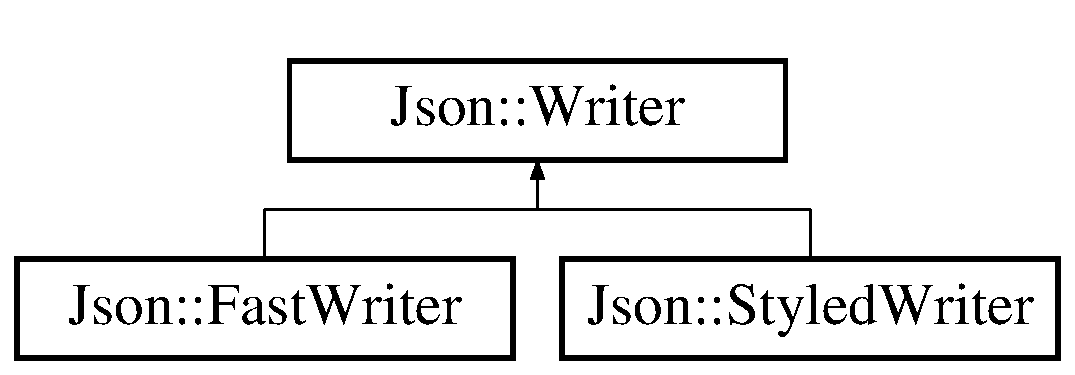
\includegraphics[height=2.000000cm]{class_json_1_1_writer}
\end{center}
\end{figure}
\subsection*{Public Member Functions}
\begin{DoxyCompactItemize}
\item 
\hypertarget{class_json_1_1_writer_a7b2273a4ffd6f32b369ac8a53b7b5a0d}{virtual std\-::string {\bfseries write} (const \hyperlink{class_json_1_1_value}{Value} \&root)=0}\label{class_json_1_1_writer_a7b2273a4ffd6f32b369ac8a53b7b5a0d}

\end{DoxyCompactItemize}


\subsection{Detailed Description}
Abstract class for writers. 

The documentation for this class was generated from the following files\-:\begin{DoxyCompactItemize}
\item 
include/json/json.\-h\item 
src/jsoncpp.\-cpp\end{DoxyCompactItemize}

\hypertarget{struct_parse_1_1y_col_cache}{\section{Parse\-:\-:y\-Col\-Cache Struct Reference}
\label{struct_parse_1_1y_col_cache}\index{Parse\-::y\-Col\-Cache@{Parse\-::y\-Col\-Cache}}
}
\subsection*{Public Attributes}
\begin{DoxyCompactItemize}
\item 
\hypertarget{struct_parse_1_1y_col_cache_a7d99a4e00555cb0ff7fb3990bb7b549e}{int {\bfseries i\-Table}}\label{struct_parse_1_1y_col_cache_a7d99a4e00555cb0ff7fb3990bb7b549e}

\item 
\hypertarget{struct_parse_1_1y_col_cache_a67bdb189ef88aca5fc30b551da9a0f90}{int {\bfseries i\-Column}}\label{struct_parse_1_1y_col_cache_a67bdb189ef88aca5fc30b551da9a0f90}

\item 
\hypertarget{struct_parse_1_1y_col_cache_a61561cab1ce2e1914083777ae84c8fe8}{u8 {\bfseries temp\-Reg}}\label{struct_parse_1_1y_col_cache_a61561cab1ce2e1914083777ae84c8fe8}

\item 
\hypertarget{struct_parse_1_1y_col_cache_a656ea77cf538db00249221de58fd9066}{int {\bfseries i\-Level}}\label{struct_parse_1_1y_col_cache_a656ea77cf538db00249221de58fd9066}

\item 
\hypertarget{struct_parse_1_1y_col_cache_aadb47e545234142bd1e9ca4803953ab0}{int {\bfseries i\-Reg}}\label{struct_parse_1_1y_col_cache_aadb47e545234142bd1e9ca4803953ab0}

\item 
\hypertarget{struct_parse_1_1y_col_cache_ac163bb2b692f3037054f92294322f999}{int {\bfseries lru}}\label{struct_parse_1_1y_col_cache_ac163bb2b692f3037054f92294322f999}

\end{DoxyCompactItemize}


The documentation for this struct was generated from the following file\-:\begin{DoxyCompactItemize}
\item 
src/sqlite3.\-c\end{DoxyCompactItemize}

\hypertarget{union_y_y_m_i_n_o_r_t_y_p_e}{\section{Y\-Y\-M\-I\-N\-O\-R\-T\-Y\-P\-E Union Reference}
\label{union_y_y_m_i_n_o_r_t_y_p_e}\index{Y\-Y\-M\-I\-N\-O\-R\-T\-Y\-P\-E@{Y\-Y\-M\-I\-N\-O\-R\-T\-Y\-P\-E}}
}
\subsection*{Public Attributes}
\begin{DoxyCompactItemize}
\item 
\hypertarget{union_y_y_m_i_n_o_r_t_y_p_e_a6cec97309f473b42b70a9738d7cbd5ba}{int {\bfseries yyinit}}\label{union_y_y_m_i_n_o_r_t_y_p_e_a6cec97309f473b42b70a9738d7cbd5ba}

\item 
\hypertarget{union_y_y_m_i_n_o_r_t_y_p_e_a827d6a1bc7ac8df062b3f419db3f50ac}{sqlite3\-Parser\-T\-O\-K\-E\-N\-T\-Y\-P\-E {\bfseries yy0}}\label{union_y_y_m_i_n_o_r_t_y_p_e_a827d6a1bc7ac8df062b3f419db3f50ac}

\item 
\hypertarget{union_y_y_m_i_n_o_r_t_y_p_e_aeb6b77e9a54a740178f47c10d2263f39}{struct \hyperlink{struct_limit_val}{Limit\-Val} {\bfseries yy64}}\label{union_y_y_m_i_n_o_r_t_y_p_e_aeb6b77e9a54a740178f47c10d2263f39}

\item 
\hypertarget{union_y_y_m_i_n_o_r_t_y_p_e_a42df0f01a945b0edd4c2d444383271c6}{\hyperlink{struct_expr}{Expr} $\ast$ {\bfseries yy122}}\label{union_y_y_m_i_n_o_r_t_y_p_e_a42df0f01a945b0edd4c2d444383271c6}

\item 
\hypertarget{union_y_y_m_i_n_o_r_t_y_p_e_a9f223bea5f91f81654ec73b44da4e9e2}{\hyperlink{struct_select}{Select} $\ast$ {\bfseries yy159}}\label{union_y_y_m_i_n_o_r_t_y_p_e_a9f223bea5f91f81654ec73b44da4e9e2}

\item 
\hypertarget{union_y_y_m_i_n_o_r_t_y_p_e_a85f445ea34e555f9fe590d7bf009ebe5}{\hyperlink{struct_id_list}{Id\-List} $\ast$ {\bfseries yy180}}\label{union_y_y_m_i_n_o_r_t_y_p_e_a85f445ea34e555f9fe590d7bf009ebe5}

\item 
\hypertarget{union_y_y_m_i_n_o_r_t_y_p_e_a62e5677bd4fe257ac60796bff10861f9}{\begin{tabbing}
xx\=xx\=xx\=xx\=xx\=xx\=xx\=xx\=xx\=\kill
struct \{\\
\>int {\bfseries value}\\
\>int {\bfseries mask}\\
\} {\bfseries yy207}}\label{union_y_y_m_i_n_o_r_t_y_p_e_a62e5677bd4fe257ac60796bff10861f9}
\\

\end{tabbing}\item 
\hypertarget{union_y_y_m_i_n_o_r_t_y_p_e_a7550aa923cb83eba5ea5ca4d2c425f36}{u8 {\bfseries yy258}}\label{union_y_y_m_i_n_o_r_t_y_p_e_a7550aa923cb83eba5ea5ca4d2c425f36}

\item 
\hypertarget{union_y_y_m_i_n_o_r_t_y_p_e_a981c25f9db81ef6dd0b1a09ae1eace9b}{struct \hyperlink{struct_like_op}{Like\-Op} {\bfseries yy318}}\label{union_y_y_m_i_n_o_r_t_y_p_e_a981c25f9db81ef6dd0b1a09ae1eace9b}

\item 
\hypertarget{union_y_y_m_i_n_o_r_t_y_p_e_a0cf3fb7c57ebedcfdfc0271524c22465}{\hyperlink{struct_trigger_step}{Trigger\-Step} $\ast$ {\bfseries yy327}}\label{union_y_y_m_i_n_o_r_t_y_p_e_a0cf3fb7c57ebedcfdfc0271524c22465}

\item 
\hypertarget{union_y_y_m_i_n_o_r_t_y_p_e_a3adf1325462a9fecaa520711ac543eb2}{\hyperlink{struct_expr_span}{Expr\-Span} {\bfseries yy342}}\label{union_y_y_m_i_n_o_r_t_y_p_e_a3adf1325462a9fecaa520711ac543eb2}

\item 
\hypertarget{union_y_y_m_i_n_o_r_t_y_p_e_ac7e3d77993d8c117ecf7274c935d6ce1}{\hyperlink{struct_src_list}{Src\-List} $\ast$ {\bfseries yy347}}\label{union_y_y_m_i_n_o_r_t_y_p_e_ac7e3d77993d8c117ecf7274c935d6ce1}

\item 
\hypertarget{union_y_y_m_i_n_o_r_t_y_p_e_a022e706c47bf19b5baedc3bd4f448784}{int {\bfseries yy392}}\label{union_y_y_m_i_n_o_r_t_y_p_e_a022e706c47bf19b5baedc3bd4f448784}

\item 
\hypertarget{union_y_y_m_i_n_o_r_t_y_p_e_aafb633841243d9820fc85ebdac0323ee}{struct \hyperlink{struct_trig_event}{Trig\-Event} {\bfseries yy410}}\label{union_y_y_m_i_n_o_r_t_y_p_e_aafb633841243d9820fc85ebdac0323ee}

\item 
\hypertarget{union_y_y_m_i_n_o_r_t_y_p_e_a60690037786cf4178493b8463f7c76d2}{\hyperlink{struct_expr_list}{Expr\-List} $\ast$ {\bfseries yy442}}\label{union_y_y_m_i_n_o_r_t_y_p_e_a60690037786cf4178493b8463f7c76d2}

\item 
\hypertarget{union_y_y_m_i_n_o_r_t_y_p_e_a565d289fa56f79ebd699d4e7decea365}{struct \hyperlink{struct_value_list}{Value\-List} {\bfseries yy487}}\label{union_y_y_m_i_n_o_r_t_y_p_e_a565d289fa56f79ebd699d4e7decea365}

\end{DoxyCompactItemize}


The documentation for this union was generated from the following file\-:\begin{DoxyCompactItemize}
\item 
src/sqlite3.\-c\end{DoxyCompactItemize}

\hypertarget{structyy_parser}{\section{yy\-Parser Struct Reference}
\label{structyy_parser}\index{yy\-Parser@{yy\-Parser}}
}
\subsection*{Public Attributes}
\begin{DoxyCompactItemize}
\item 
\hypertarget{structyy_parser_a19abcf4780515fd2debd1ce7a2e29f95}{int {\bfseries yyidx}}\label{structyy_parser_a19abcf4780515fd2debd1ce7a2e29f95}

\item 
\hypertarget{structyy_parser_ac0350933aa515a3a756dfa742d04ee59}{int {\bfseries yyerrcnt}}\label{structyy_parser_ac0350933aa515a3a756dfa742d04ee59}

\item 
\hypertarget{structyy_parser_ae8bc1531d6ae56020a7ee33a40783672}{sqlite3\-Parser\-A\-R\-G\-\_\-\-S\-D\-E\-C\-L \hyperlink{structyy_stack_entry}{yy\-Stack\-Entry} {\bfseries yystack} \mbox{[}Y\-Y\-S\-T\-A\-C\-K\-D\-E\-P\-T\-H\mbox{]}}\label{structyy_parser_ae8bc1531d6ae56020a7ee33a40783672}

\end{DoxyCompactItemize}


The documentation for this struct was generated from the following file\-:\begin{DoxyCompactItemize}
\item 
src/sqlite3.\-c\end{DoxyCompactItemize}

\hypertarget{structyy_stack_entry}{\section{yy\-Stack\-Entry Struct Reference}
\label{structyy_stack_entry}\index{yy\-Stack\-Entry@{yy\-Stack\-Entry}}
}
\subsection*{Public Attributes}
\begin{DoxyCompactItemize}
\item 
\hypertarget{structyy_stack_entry_a108164609c2e841577cc3533d8f0180d}{Y\-Y\-A\-C\-T\-I\-O\-N\-T\-Y\-P\-E {\bfseries stateno}}\label{structyy_stack_entry_a108164609c2e841577cc3533d8f0180d}

\item 
\hypertarget{structyy_stack_entry_a7624d02bcf945d48068f4c383551725c}{Y\-Y\-C\-O\-D\-E\-T\-Y\-P\-E {\bfseries major}}\label{structyy_stack_entry_a7624d02bcf945d48068f4c383551725c}

\item 
\hypertarget{structyy_stack_entry_a024e1e64bce5945080629a2dd8d1bb4f}{\hyperlink{union_y_y_m_i_n_o_r_t_y_p_e}{Y\-Y\-M\-I\-N\-O\-R\-T\-Y\-P\-E} {\bfseries minor}}\label{structyy_stack_entry_a024e1e64bce5945080629a2dd8d1bb4f}

\end{DoxyCompactItemize}


The documentation for this struct was generated from the following file\-:\begin{DoxyCompactItemize}
\item 
src/sqlite3.\-c\end{DoxyCompactItemize}

\addcontentsline{toc}{part}{Index}
\printindex
\end{document}
